\documentclass{book}
\usepackage[a4paper,top=2.5cm,bottom=2.5cm,left=2.5cm,right=2.5cm]{geometry}
\usepackage{makeidx}
\usepackage{natbib}
\usepackage{graphicx}
\usepackage{multicol}
\usepackage{float}
\usepackage{listings}
\usepackage{color}
\usepackage{ifthen}
\usepackage[table]{xcolor}
\usepackage{textcomp}
\usepackage{alltt}
\usepackage{ifpdf}
\ifpdf
\usepackage[pdftex,
            pagebackref=true,
            colorlinks=true,
            linkcolor=blue,
            unicode
           ]{hyperref}
\else
\usepackage[ps2pdf,
            pagebackref=true,
            colorlinks=true,
            linkcolor=blue,
            unicode
           ]{hyperref}
\usepackage{pspicture}
\fi
\usepackage[utf8]{inputenc}
\usepackage{mathptmx}
\usepackage[scaled=.90]{helvet}
\usepackage{courier}
\usepackage{sectsty}
\usepackage{amssymb}
\usepackage[titles]{tocloft}
\usepackage{doxygen}
\lstset{language=C++,inputencoding=utf8,basicstyle=\footnotesize,breaklines=true,breakatwhitespace=true,tabsize=8,numbers=left }
\makeindex
\setcounter{tocdepth}{3}
\renewcommand{\footrulewidth}{0.4pt}
\renewcommand{\familydefault}{\sfdefault}
\hfuzz=15pt
\setlength{\emergencystretch}{15pt}
\hbadness=750
\tolerance=750
\begin{document}
\hypersetup{pageanchor=false,citecolor=blue}
\begin{titlepage}
\vspace*{7cm}
\begin{center}
{\Large faudio v2.8.1 }\\
\vspace*{1cm}
{\large Generated by Doxygen 1.8.3}\\
\vspace*{0.5cm}
{\small Wed Jan 29 2014 14:49:38}\\
\end{center}
\end{titlepage}
\clearemptydoublepage
\pagenumbering{roman}
\tableofcontents
\clearemptydoublepage
\pagenumbering{arabic}
\hypersetup{pageanchor=true,citecolor=blue}
\chapter{Introduction}
\label{index}\hypertarget{index}{}{\itshape faudio} is a high-\/level, declarative audio engine written in A\-N\-S\-I C.

Main features\-:


\begin{DoxyItemize}
\item Real-\/time and non-\/realtime processing.
\item Arbitrary number of streams in the same process.
\item Device detection/hot-\/plugging.
\item Arbitrary complex audio routing.
\item High-\/level interface, using declarative {\itshape signals}. 
\end{DoxyItemize}
\chapter{Build and install}
\label{md_Build_and_install}
\hypertarget{md_Build_and_install}{}
\hypertarget{md__build_and_install_Prerequisites}{}\section{Prerequisites}\label{md__build_and_install_Prerequisites}
\label{md__build_and_install_Prerequisites}%
\hypertarget{md__build_and_install_Prerequisites}{}%


The following tools and libraries are required to build {\itshape faudio}.\hypertarget{md__build_and_install_Platform}{}\section{Platform}\label{md__build_and_install_Platform}
Supported platforms are\-:


\begin{DoxyItemize}
\item Windows X\-P or later
\item Mac O\-S X 10.\-5 or later
\end{DoxyItemize}

Porting to Linux should be relatively easy but has not been done yet.\hypertarget{md__build_and_install_Compiler}{}\subsection{Compiler}\label{md__build_and_install_Compiler}
A compiler supporting the C99 standard is required. Currently tested are\-:


\begin{DoxyItemize}
\item clang 3.\-1 or later (Apple call this compiler \char`\"{}4.\-0.\-0 based of S\-V\-N 3.\-1\char`\"{})
\item G\-C\-C 4.\-6.\-2 or later
\end{DoxyItemize}

The default Windows compiler (Visual C/\-C++) is not well supported, the Min\-G\-W version of G\-C\-C is recommended.\hypertarget{md__build_and_install_Tools}{}\subsection{Tools}\label{md__build_and_install_Tools}
The following tools are required to build {\itshape faudio}.

\subsubsection*{C\-Make}

\href{http://www.cmake.org}{\tt http\-://www.\-cmake.\-org}

Required for building the libraries and binaries.

At present the {\itshape only} supported generators are Makefiles on Linux O\-S X, and M\-S\-Y\-S Makefiles on Windows. Cygwin Makefiles {\itshape might} work, but is not well tested, and not recommended as the Cygwin compiler might not generate standard Windows binaries.

\subsubsection*{Modulo}

\href{https://github.com/hanshoglund/modulo}{\tt https\-://github.\-com/hanshoglund/modulo}

Required for generating headers and low-\/level language bindings.

\subsubsection*{Doxygen}

\href{http://www.stack.nl/~dimitri/doxygen}{\tt http\-://www.\-stack.\-nl/$\sim$dimitri/doxygen}

Required for generating the documentation.

\subsubsection*{Graph\-Viz}

\href{http://www.graphviz.org/}{\tt http\-://www.\-graphviz.\-org/}

Optionally used for generating graphs.

\subsubsection*{gnuplot}

\href{http://gnuplot.sourceforge.net/}{\tt http\-://gnuplot.\-sourceforge.\-net/}

Optionally used for generating plots.

\subsubsection*{Image\-Magick}

\href{http://www.imagemagick.org/script/index.php}{\tt http\-://www.\-imagemagick.\-org/script/index.\-php}

Optionally used for converting graphs.

\subsubsection*{Ghost\-Script}

\href{http://pages.cs.wisc.edu/~ghost/}{\tt http\-://pages.\-cs.\-wisc.\-edu/$\sim$ghost/}

Optionally used for converting plots.

\subsubsection*{G\-N\-U Make}

Required for building language bindings and documentation.\hypertarget{md__build_and_install_Libraries}{}\subsection{Libraries}\label{md__build_and_install_Libraries}
\label{md__build_and_install_Libraries}%
\hypertarget{md__build_and_install_Libraries}{}%
 These are typically handled by the package mangager, see build and install.

\subsubsection*{Portaudio}

\href{http://www.portaudio.com}{\tt http\-://www.\-portaudio.\-com} \href{http://portmedia.sourceforge.net}{\tt http\-://portmedia.\-sourceforge.\-net}

Required for real-\/time audio streams on all systems.

\subsubsection*{Portmidi}

\href{http://portmedia.sourceforge.net}{\tt http\-://portmedia.\-sourceforge.\-net}

Required for real-\/time midi streams on all systems.

\subsubsection*{Libsndfile}

\href{http://www.mega-nerd.com/libsndfile}{\tt http\-://www.\-mega-\/nerd.\-com/libsndfile}

Required for non-\/real-\/time audio streams on all systems.

\subsubsection*{Fluidsynth}

\href{http://sourceforge.net/apps/trac/fluidsynth}{\tt http\-://sourceforge.\-net/apps/trac/fluidsynth}

Required for using the Fluidsynth audio processor.\hypertarget{md__build_and_install_BasicBuild}{}\section{Basic build}\label{md__build_and_install_BasicBuild}
First ensure that your system meets the \hyperlink{md__build_and_install_Platform}{platform} requirements, and that the necessary \hyperlink{md__build_and_install_Compiler}{compiler} and \hyperlink{md__build_and_install_Tools}{tools} are available.

The source code for {\itshape faudio} can be obtained by. \begin{DoxyVerb}$ git clone git@github.com:faudio/faudio.git
$ cd audio-engine
\end{DoxyVerb}


After changing into the {\ttfamily audio-\/engine} directory, the {\ttfamily bootstrap} script should be run. This will create a standard out-\/of-\/source build in the {\ttfamily build} subdirectory. After a successful bootstrap, you can run {\ttfamily make help} to view build commands or {\ttfamily make} to perform the build.

All in all, the simplest possible build session looks like this\-: \begin{DoxyVerb}$ ./bootstrap [options]
$ make
$ make test
\end{DoxyVerb}
\hypertarget{md__build_and_install_AdvancedBuild}{}\section{Advanced build}\label{md__build_and_install_AdvancedBuild}
\hypertarget{md__build_and_install_Dependencies}{}\subsection{Building local dependencies}\label{md__build_and_install_Dependencies}
The bootstrap script automatically downloads the \hyperlink{md__build_and_install_Libraries}{required libraries}. You can also build libraries locally, using the component commands described below.\hypertarget{md__build_and_install_SettingOptions}{}\subsection{Setting and inspecting options}\label{md__build_and_install_SettingOptions}
Build options can be changed using any C\-Make tool, such as {\ttfamily cmake-\/gui} or {\ttfamily ccmake}.

You can also change a build setting on the command line. These changes will persist until you change them again, or regenerate the build directory. \begin{DoxyVerb}$ cmake build -DMY_SETTING=0
\end{DoxyVerb}
\hypertarget{md__build_and_install_SeparateBuildDir}{}\subsection{Using a separate build directory}\label{md__build_and_install_SeparateBuildDir}
If you use {\ttfamily ccmake} or {\ttfamily cmake-\/gui} you should run them on the {\ttfamily build} directory, which is the default build directory created by the bootstrap script.

If you want to use another build directory, i.\-e. for maintaining multiple builds of the same source, you can rerun the bootstrap script passing the {\ttfamily B\-U\-I\-L\-D\-\_\-\-D\-I\-R\-E\-C\-T\-O\-R\-Y} flag. \begin{DoxyVerb}$ BUILD_DIRECTORY=my_build_dir ./bootstrap
\end{DoxyVerb}
\hypertarget{md__build_and_install_Rebuilding}{}\section{Rebuilding headers and bindings}\label{md__build_and_install_Rebuilding}
T\-O\-D\-O\hypertarget{md__build_and_install_Running}{}\section{Running and testing}\label{md__build_and_install_Running}
T\-O\-D\-O\hypertarget{md__build_and_install_Distributing}{}\section{Distributing the build}\label{md__build_and_install_Distributing}
T\-O\-D\-O\hypertarget{md__build_and_install_Reference}{}\section{Reference}\label{md__build_and_install_Reference}
\hypertarget{md__build_and_install_Options}{}\subsection{Options}\label{md__build_and_install_Options}
\begin{TabularC}{2}
\hline
\rowcolor{lightgray}{\bf Name }&{\bf Description}\\\cline{1-2}
C\-M\-A\-K\-E\-\_\-\-B\-U\-I\-L\-D\-\_\-\-T\-Y\-P\-E &Either {\ttfamily Debug}, {\ttfamily Release} or {\ttfamily Rel\-With\-Deb\-Info} \\\cline{1-2}
E\-N\-A\-B\-L\-E\-\_\-\-R\-E\-A\-L\-T\-I\-M\-E\-\_\-\-A\-U\-D\-I\-O &Enable real-\/time audio \\\cline{1-2}
E\-N\-A\-B\-L\-E\-\_\-\-R\-E\-A\-L\-T\-I\-M\-E\-\_\-\-M\-I\-D\-I &Enable real-\/time midi \\\cline{1-2}
E\-N\-A\-B\-L\-E\-\_\-\-N\-O\-N\-R\-E\-A\-L\-T\-I\-M\-E\-\_\-\-A\-U\-D\-I\-O &Enable non-\/real-\/time audio \\\cline{1-2}
E\-N\-A\-B\-L\-E\-\_\-\-F\-L\-U\-I\-D\-S\-Y\-N\-T\-H &Enable the Fluid\-Synth processor \\\cline{1-2}
E\-N\-A\-B\-L\-E\-\_\-\-A\-U\-D\-I\-O\-\_\-\-U\-N\-I\-T &Enable Audio\-Unit processors \\\cline{1-2}
E\-N\-A\-B\-L\-E\-\_\-\-V\-S\-T &Enable V\-S\-T processors \\\cline{1-2}
B\-U\-I\-L\-D\-\_\-\-F\-R\-A\-M\-E\-W\-O\-R\-K &Build an O\-S X framework \\\cline{1-2}
B\-U\-I\-L\-D\-\_\-\-S\-H\-A\-R\-E\-D &Build a shared library \\\cline{1-2}
B\-U\-I\-L\-D\-\_\-\-T\-E\-S\-T\-S &Build unit tests \\\cline{1-2}
P\-R\-O\-F\-I\-L\-I\-N\-G &Compile with profiler flags -\/pg set \\\cline{1-2}
B\-U\-I\-L\-D\-\_\-\-C\-O\-M\-P\-O\-N\-E\-N\-T\-S &Build dependent components locally \\\cline{1-2}
S\-H\-O\-W\-\_\-\-C\-O\-M\-P\-O\-N\-E\-N\-T\-\_\-\-O\-U\-T\-P\-U\-T &Show output while building components \\\cline{1-2}
\end{TabularC}
\hypertarget{md__build_and_install_Commands}{}\subsection{Commands}\label{md__build_and_install_Commands}
The build commands should always be run from the top directory. They will delegate to the {\ttfamily build} directory by default. You can use the {\ttfamily B\-U\-I\-L\-D\-\_\-\-D\-I\-R\-E\-C\-T\-O\-R\-Y} flag to override. \begin{DoxyVerb}make test
\end{DoxyVerb}


This command builds and runs the standard test suite. This may take several minutes to complete. \begin{DoxyVerb}make modules
\end{DoxyVerb}


This command builds most of the headers in the {\ttfamily include/} subdirectory. \begin{DoxyVerb}make bindings
\end{DoxyVerb}


This command builds the external language bindings in the {\ttfamily bindings/} subdirectory. \begin{DoxyVerb}make doc
\end{DoxyVerb}


This command builds documentation in the {\ttfamily doc/build} subdirectory. By default both H\-T\-M\-L and P\-D\-F files are produced. \begin{DoxyVerb}make dist\end{DoxyVerb}
 
\chapter{Data structures}
\label{md_Data_structures}
\hypertarget{md_Data_structures}{}
\label{md__data_structures_DataStructures}%
\hypertarget{md__data_structures_DataStructures}{}%


{\itshape faudio} include a set of general purpose \href{http://en.wikipedia.org/wiki/Persistent_data_structure}{\tt persistent~data~structures}, which are primarily used for message passing between the audio thread and other threads. The fact that the data structures are persistent eliminate many of the problems commonly associated with multi-\/threaded programming.

The data structures in {\itshape faudio} are somewhat different from the structures found in most languages, in that they have single-\/ownership semantics. This eliminates the need for a garbage collector while still allowing a high-\/level programming style. To understand single-\/ownership semantics, you should read the section about \hyperlink{md__data_structures_CreateCopyDestroy}{creation~and~destruction} below. All data structures are polymorphic over reference types, see the section on \hyperlink{md__data_structures_id19466}{type~safety} for more details.

Note that there is no interface capturing the notion of a data structure\-: they are simply reference types obeying the conventions described below. However, all data structures support generic \hyperlink{structfa__equal__t}{equality} or \hyperlink{structfa__order__t}{ordering}, \hyperlink{structfa__copy__t}{copying} and \hyperlink{structfa__destroy__t}{destruction}.\hypertarget{md__data_structures_Overview}{}\section{Overview}\label{md__data_structures_Overview}
The core data structures are\-:

\begin{TabularC}{2}
\hline
\rowcolor{lightgray}{\bf Type }&{\bf Semantics}\\\cline{1-2}
\hyperlink{group___fa_pair}{Pair} &An ordered pair \\\cline{1-2}
\hyperlink{group___fa_list}{List} &An ordered sequence \\\cline{1-2}
Set &An ordered set \\\cline{1-2}
\hyperlink{group___fa_map}{Map} &A set of ordered pairs \\\cline{1-2}
\hyperlink{group___fa_string}{String} &A sequence of Unicode characters \\\cline{1-2}
\end{TabularC}


There is also a set of {\itshape mutable} data structures not included in this table. These are used internally in {\itshape faudio} and need rarely be accessed by the user. For completeness, they are\-:

\begin{TabularC}{2}
\hline
\rowcolor{lightgray}{\bf Type }&{\bf Semantics}\\\cline{1-2}
\hyperlink{group___fa_atomic}{Atomic} &An atomic reference \\\cline{1-2}
\hyperlink{group___fa_atomic_queue}{Atomic queue} &A first-\/in, first-\/out atomic queue \\\cline{1-2}
\hyperlink{group___fa_atomic_stack}{Atomic stack} &A last-\/in, first-\/out atomic queue \\\cline{1-2}
\hyperlink{group___fa_buffer}{Buffer} &A byte-\/level mutable buffer \\\cline{1-2}
\end{TabularC}
\hypertarget{md__data_structures_Conventions}{}\section{Using data structures}\label{md__data_structures_Conventions}
\hypertarget{md__data_structures_CreateCopyDestroy}{}\subsection{Creation and destruction}\label{md__data_structures_CreateCopyDestroy}
T\-O\-D\-O\hypertarget{md__data_structures_Literals}{}\subsection{Creating from strings}\label{md__data_structures_Literals}
\subsubsection*{Show}

When \hyperlink{group___fa_ga60d1e34d8101c4f20d7e5473c90766a2}{printed}, the data structures are rendered in a language-\/neutral form.


\begin{DoxyItemize}
\item {\ttfamily (1,2)}
\item {\ttfamily \mbox{[}1,2,3\mbox{]}}
\item {\ttfamily \{1,2,3\}}
\item {\ttfamily \{foo\-:1,bar\-:2\}}
\item {\ttfamily (\{1,2,3\},\{((1,2),\char`\"{}foo\char`\"{}),((1,3)\-:\char`\"{}bar\char`\"{})\})}
\end{DoxyItemize}

\subsubsection*{Literals}

All data structures have {\itshape literals} defined in the \hyperlink{literals_8h}{utility~headers}. A literal expression always evaluate to a newly created instance of the data structure. Beware not to pass a number to the literals, you must use \hyperlink{md__data_structures_ValueReferences}{value~references}.


\begin{DoxyItemize}
\item {\ttfamily pair(\hyperlink{util_8h_a832509ea197065489f1d60b6d7958cbf}{i32(1)},\hyperlink{util_8h_a832509ea197065489f1d60b6d7958cbf}{i32(2)})}
\item {\ttfamily list(\hyperlink{util_8h_a832509ea197065489f1d60b6d7958cbf}{i32(1)},\hyperlink{util_8h_a832509ea197065489f1d60b6d7958cbf}{i32(2)},\hyperlink{util_8h_a832509ea197065489f1d60b6d7958cbf}{i32(3)})}
\item {\ttfamily set(\hyperlink{util_8h_a832509ea197065489f1d60b6d7958cbf}{i32(1)},\hyperlink{util_8h_a832509ea197065489f1d60b6d7958cbf}{i32(2)},\hyperlink{util_8h_a832509ea197065489f1d60b6d7958cbf}{i32(3)})}
\item {\ttfamily map(string(\char`\"{}foo\char`\"{}),\hyperlink{util_8h_a832509ea197065489f1d60b6d7958cbf}{i32(1)},string(\char`\"{}bar\char`\"{}),\hyperlink{util_8h_a832509ea197065489f1d60b6d7958cbf}{i32(2)})}
\item {\ttfamily graph(\hyperlink{util_8h_a832509ea197065489f1d60b6d7958cbf}{i32(1)},\hyperlink{util_8h_a832509ea197065489f1d60b6d7958cbf}{i32(2)},edge(\hyperlink{util_8h_a832509ea197065489f1d60b6d7958cbf}{i32(1)},\hyperlink{util_8h_a832509ea197065489f1d60b6d7958cbf}{i32(2)},\hyperlink{util_8h_a832509ea197065489f1d60b6d7958cbf}{i32(3)}))}
\end{DoxyItemize}

\subsubsection*{J\-S\-O\-N}

T\-O\-D\-O\hypertarget{md__data_structures_ForEach}{}\subsection{Accessing all elements}\label{md__data_structures_ForEach}
T\-O\-D\-O\hypertarget{md__data_structures_MapFoldFilter}{}\subsection{Mapping, folding and filtering}\label{md__data_structures_MapFoldFilter}
T\-O\-D\-O\hypertarget{md__data_structures_ThreadSafety}{}\subsection{Thread safety}\label{md__data_structures_ThreadSafety}
All operations on data structures are thread-\/safe except creation, copying and destruction, which are subject to the following restrictions\-:


\begin{DoxyItemize}
\item If a data structure {\itshape a} is created in thread {\itshape t} and used in thread {\itshape u}, an ordering must be established between the creation function returning in {\itshape t} and subsequent use of {\itshape a} in {\itshape u}.
\end{DoxyItemize}


\begin{DoxyItemize}
\item If a data structure {\itshape a} is used in thread {\itshape t} and destroyed in thread {\itshape u}, an ordering must be established between the last use of {\itshape a} in {\itshape t} and the destructive function being applied in {\itshape u}.
\end{DoxyItemize}

To establish an ordering, you should either synchronize the threads {\itshape t} and {\itshape u}, or transfer the data structure in an atomic variable or queue. Note that copying is considered both {\itshape usage} of the copied value and a {\itshape creation} of the copy. Also some functions (such as \hyperlink{group___fa_list_ga29aba2e79fd9c128c05d020be5a3b254}{fa\-\_\-list\-\_\-dcons}) are both destructive on its input, and constructive on its output.\hypertarget{md__data_structures_id19466}{}\subsection{Type safety}\label{md__data_structures_id19466}
All data structures can store all reference types, including \hyperlink{md__data_structures_ValueReferences}{value~references}. The user must rely on guarantees outside the scope of the compiler to assure that the extracted elements are of the right type. There are several ways to do this\-:


\begin{DoxyItemize}
\item Assure that the structure contains a specific type.
\begin{DoxyItemize}
\item For example, many functions in {\itshape faudio} A\-P\-I return pairs and lists, their documentation clearly stating what type of elements the list will contain.
\end{DoxyItemize}
\item Assure that the structure contains a generic type.
\begin{DoxyItemize}
\item For example, a function may require a set of values implementing \hyperlink{structfa__string__show__t}{Show}.
\end{DoxyItemize}
\end{DoxyItemize}

In some cases, it does not matter what type a data structure contains, as the elements are not going to be inspected. For example, \hyperlink{group___fa_list_ga7b187ef70819a17992b0d787683de241}{fa\-\_\-list\-\_\-reverse} can receive a list of any type, as it operates purely on the structure of the list and does not need to use its values.\hypertarget{md__data_structures_id182783728273}{}\section{Value references}\label{md__data_structures_id182783728273}
\label{md__data_structures_ValueReferences}%
\hypertarget{md__data_structures_ValueReferences}{}%
 Value types can be converted to reference types using a set of conversion functions. These functions take a non reference type and return a so called {\itshape value reference}. This reference can subsequently be destroyed and its value extracted.

A value reference is a proper reference that can be safely stored in a data structure. Like other data structures, value references may be created and destroyed from any thread and have single ownership semantics. Value references are in fact tiny data structures containing a single element. They support all normal data structure operations including \hyperlink{structfa__equal__t}{equality} or \hyperlink{structfa__order__t}{ordering}, \hyperlink{structfa__copy__t}{copying} and \hyperlink{structfa__destroy__t}{destruction}. In addition, they also support \hyperlink{structfa__number__t}{arithmetic}.

It is not specified exactly how value references are implemented; however the reference representation of a value typically have a different bit pattern from the represented value. It is not safe to cast a value of a primitive type, such as an integer, to a pointer and treat the resulting address as a value reference. Conversely, it is not safe to treat a value reference as a pointer by dereferencing it, or doing pointer arithmetic. It is guaranteed that the value references will never overlap with real references. 
\chapter{Devices}
\label{md_Devices}
\hypertarget{md_Devices}{}
\label{md__devices_Devices}%
\hypertarget{md__devices_Devices}{}%


Devices are the entities that allow {\itshape faudio} to communicate with the outside world. Any client will need to connect at least two devices to each other to form a audio stream. While signals and processors denote functions, devices denote sources and sinks of audio data, such as files, memory buffers or audio hardware.

Devices are grouped into {\itshape real-\/time devices}, {\itshape non-\/real-\/time devices}. Audio and midi information are handled by different devices. Note that {\itshape faudio} does not provide non-\/real-\/time midi at the moment\-: if you need to parse and process a midi file you must use some other method.\hypertarget{md__devices_RealTime}{}\section{Real time devices}\label{md__devices_RealTime}
\hypertarget{md__devices_SessionsAndStreams}{}\subsection{Sessions and streams}\label{md__devices_SessionsAndStreams}
{\itshape faudio} provides access to real-\/time devices through of {\itshape sessions}, and {\itshape streams}. While a {\itshape device} provides access to an external audio interface, a {\itshape session} provides access to the entire audio system, and a {\itshape stream} to a specific audio computation. These concepts are hierarchical, each stream is associated with a device and each device with a session.

Typically, each physical audio or midi interface is represented by a single device in {\itshape faudio}. The operating system may also provide abstract devices, representing network connections, software mixers and the like.

{\itshape faudio} places certain restrictions on the order or acquisition of sessions, devices and streams. Any client that wants to obtain a device must first initiate a session. The initialization of a session may fail, for example if the underlying audio system is already being used by an exclusive process. If it succeeds, a handle to the underlying session is provided. This handle allow the user to inspect the set of devices available in the sesssion. The client may then open a stream.

T\-O\-D\-O


\begin{DoxyImage}
\includegraphics[width=0.8\textwidth]{device_states}
\caption{State transactions of the audio system (simplified)}
\end{DoxyImage}


\begin{DoxyNote}{Note}
The semantics of {\itshape streams} have been changed from earlier versions of {\itshape faudio}, in which a {\itshape stream} could be repeatedly stopped and started.
\end{DoxyNote}
\hypertarget{md__devices_Notifications}{}\subsection{Session notifications}\label{md__devices_Notifications}
Sessions represent a snapshot of the setup at the time it was initiated; the set of available devices in a specific session will never change. If a change in the underlying audio system is detected while a session is still active, a new session has to be started to observe the new setup.

You can register a callback to be invoked when the a possible change in hardware setup is detected, see fa\-\_\-\-\_\-audio\-\_\-set\-\_\-status\-\_\-callback. Note that this callback may be invoked in an interrupt handler thread and that the task of ending a session should generally be handled in the same thread that created the session. Use an atomic reference or a condition variable to communicate the notification to the appropriate thread.\hypertarget{md__devices_AudioStreams}{}\subsection{Audio streams}\label{md__devices_AudioStreams}
\hypertarget{md__devices_AudioAR}{}\subsubsection{Imperative style}\label{md__devices_AudioAR}
The acquire-\/release style use a paired method pattern. You call a creation method to get a value, and a destruction method to release. Note that devices, sessions and streams have single-\/ownership semantics.


\begin{DoxyCode}
\textcolor{preprocessor}{#include <\hyperlink{fa_2fa_8h}{fa/fa.h}>}

\textcolor{keywordtype}{int} main (\textcolor{keywordtype}{int} argc, \textcolor{keywordtype}{char} \textcolor{keyword}{const} *argv[])
\{
    \hyperlink{group___fa_audio_session_ga62ee22268c23f1b18447141feccc01e0}{fa\_audio\_session\_t}     session;
    \hyperlink{group___fa_audio_device_ga03de89ee66c6465f8cedd3a0286598f4}{fa\_audio\_device\_t}      input, output;
    \hyperlink{group___fa_audio_stream_ga78fbee3026130ce00d8e00a4e73a84c3}{fa\_audio\_stream\_t}      stream
    \hyperlink{group___fa_signal_gac5c72f160cd6e93a6783551627b166e5}{fa\_signal\_t}            id;

    \textcolor{comment}{// Processor to use}
    \textcolor{keywordtype}{id} = fa\_signal\_identity();

    \textcolor{comment}{// Begin session}
    session = \hyperlink{group___fa_audio_session_ga0022e6e72ee2f2c4c04a6165847a50dd}{fa\_audio\_begin\_session}();
    \textcolor{keywordflow}{if} (\hyperlink{group___fa_gaec61e23c174faf5e5244ae876d264eb5}{fa\_check}(stream)) \{
        \hyperlink{group___fa_error_ga466e0539bedb29f68527448ed9ba11bf}{fa\_error\_log}(stream);
        \textcolor{keywordflow}{goto} cleanup;

    \} \textcolor{keywordflow}{else} \{
        \textcolor{comment}{// Session obtained, we can now access devices}
        input  = \hyperlink{group___fa_audio_device_ga690374b4ffcee314cb4cdad6309ef817}{fa\_audio\_default\_input}(session);
        input  = \hyperlink{group___fa_audio_device_ga364583565c9405e541ae52e41efa38e7}{fa\_audio\_default\_output}(session);

        \textcolor{comment}{// Start stream}
        stream = \hyperlink{group___fa_audio_stream_ga912f03969d6207dd40a2746e62888adb}{fa\_audio\_open\_stream}(input, \textcolor{keywordtype}{id}, output);
        \textcolor{keywordflow}{if} (\hyperlink{group___fa_gaec61e23c174faf5e5244ae876d264eb5}{fa\_check}(stream)) \{
            \hyperlink{group___fa_error_ga466e0539bedb29f68527448ed9ba11bf}{fa\_error\_log}(stream);
            \textcolor{keywordflow}{goto} cleanup;

        \} \textcolor{keywordflow}{else} \{
            \textcolor{comment}{// Stream active, let it run for 5 seconds}
            \hyperlink{group___fa_thread_ga6a6c70317be48603d0316bdb93914f5f}{fa\_thread\_sleep}(5000);
        \}
    \}

    \textcolor{comment}{// Cleanup}
cleanup:
    \hyperlink{group___fa_ga6fd6818b190b9e41a3b5f07e78638539}{fa\_destroy}(stream);
    \hyperlink{group___fa_ga6fd6818b190b9e41a3b5f07e78638539}{fa\_destroy}(session);
    \hyperlink{group___fa_ga6fd6818b190b9e41a3b5f07e78638539}{fa\_destroy}(\textcolor{keywordtype}{id});
\}
\end{DoxyCode}
\hypertarget{md__devices_AudioCB}{}\subsubsection{Callback style}\label{md__devices_AudioCB}
The callback style require that you provide a callback to be invoked when the session or stream is valid. Destruction is handled automatically after this method has returned. Errors are handled by a special callback, to which you can pass \hyperlink{group___fa_error_ga466e0539bedb29f68527448ed9ba11bf}{fa\-\_\-error\-\_\-log}, or a user defined function.


\begin{DoxyCode}
\textcolor{preprocessor}{#include <\hyperlink{fa_2fa_8h}{fa/fa.h}>}
\textcolor{preprocessor}{#include <\hyperlink{util_8h}{fa/util.h}>}

stream\_t run\_callback(stream\_t stream)
\{
    \textcolor{comment}{// Stream active, let it run for 5 seconds}
    \hyperlink{group___fa_thread_ga6a6c70317be48603d0316bdb93914f5f}{fa\_thread\_sleep}(\hyperlink{util_8h_a1a3cd4cff330c981ed89bbd3a3426273}{seconds}(10));
    \textcolor{keywordflow}{return} stream;
\}

session\_t session\_callback(\textcolor{keywordtype}{void}* data, session\_t session)
\{
    \hyperlink{group___fa_audio_device_ga03de89ee66c6465f8cedd3a0286598f4}{fa\_audio\_device\_t}    input, output;
    \hyperlink{group___fa_signal_gac5c72f160cd6e93a6783551627b166e5}{fa\_signal\_t}          id;

    \textcolor{comment}{// Session obtained, we can now access devices}
    input   = \hyperlink{group___fa_audio_device_ga690374b4ffcee314cb4cdad6309ef817}{fa\_audio\_default\_input}(session);
    output  = \hyperlink{group___fa_audio_device_ga690374b4ffcee314cb4cdad6309ef817}{fa\_audio\_default\_input}(session);
    \textcolor{keywordtype}{id}      = (signal\_t*) data;

    \textcolor{comment}{// Start stream}
    \hyperlink{group___fa_audio_stream_gaa385a92b31401915477027e03a39094e}{fa\_audio\_with\_stream}(input, \textcolor{keywordtype}{id}, output,
                          run\_callback, \hyperlink{group___fa_error_ga466e0539bedb29f68527448ed9ba11bf}{fa\_error\_log}, NULL);

    \hyperlink{group___fa_ga6fd6818b190b9e41a3b5f07e78638539}{fa\_destroy}(\textcolor{keywordtype}{id});
    \textcolor{keywordflow}{return} session;
\}

\textcolor{keywordtype}{int} main (\textcolor{keywordtype}{int} argc, \textcolor{keywordtype}{char} \textcolor{keyword}{const} *argv[])
\{                  
    \textcolor{comment}{// Processor to use}
    \hyperlink{group___fa_signal_gac5c72f160cd6e93a6783551627b166e5}{fa\_signal\_t} signal = fa\_signal\_identity();

    \textcolor{comment}{// Begin session}
    \hyperlink{group___fa_audio_session_gabbec6678e24f6476ac04f7d759ec7ffb}{fa\_audio\_with\_session}(session\_callback, \textcolor{keywordtype}{id},
                           \hyperlink{group___fa_error_ga466e0539bedb29f68527448ed9ba11bf}{fa\_error\_log}, NULL);
\}
\end{DoxyCode}
\hypertarget{md__devices_id8127832}{}\section{Non-\/realtime devices}\label{md__devices_id8127832}
\hypertarget{md__devices_id98281723}{}\subsection{The run method}\label{md__devices_id98281723}
T\-O\-D\-O\hypertarget{md__devices_id9192746}{}\subsection{File devices}\label{md__devices_id9192746}

\begin{DoxyCode}
\textcolor{preprocessor}{#include <\hyperlink{fa_2fa_8h}{fa/fa.h}>}

\textcolor{keyword}{typedef} fa\_file\_t      device\_t;
\textcolor{keyword}{typedef} \hyperlink{group___fa_signal_gac5c72f160cd6e93a6783551627b166e5}{fa\_signal\_t}    \hyperlink{util_8h_a4179e0566b0727e21f1fd4b5e6533dee}{signal\_t};

\textcolor{keywordtype}{int} main (\textcolor{keywordtype}{int} argc, \textcolor{keywordtype}{char} \textcolor{keyword}{const} *argv[])
\{
    fa\_device\_t    input, output;
    \hyperlink{group___fa_signal_gac5c72f160cd6e93a6783551627b166e5}{fa\_signal\_t}    id;
    fa\_result\_t    result;

    \textcolor{comment}{// Processor to use}
    \textcolor{keywordtype}{id} = fa\_signal\_identity();

    \textcolor{comment}{// Open streams}
    input   = fa\_\_file\_open(\textcolor{keywordtype}{string}(\textcolor{stringliteral}{"test/in.wav"}));
    output  = fa\_\_file\_open(\textcolor{keywordtype}{string}(\textcolor{stringliteral}{"test/out.wav"}));

    \textcolor{comment}{// Handle possible errors}
    \textcolor{keywordflow}{if} (\hyperlink{group___fa_gaec61e23c174faf5e5244ae876d264eb5}{fa\_check}(input)) \{
        \hyperlink{group___fa_error_ga466e0539bedb29f68527448ed9ba11bf}{fa\_error\_log}(result);
    \}                                    

    \textcolor{keywordflow}{if} (\hyperlink{group___fa_gaec61e23c174faf5e5244ae876d264eb5}{fa\_check}(output)) \{
        \hyperlink{group___fa_error_ga466e0539bedb29f68527448ed9ba11bf}{fa\_error\_log}(result);
    \}                                    

    result  = fa\_\_file\_run(in, \textcolor{keywordtype}{id}, out);

    \textcolor{comment}{// Handle possible error}
    \textcolor{keywordflow}{if} (\hyperlink{group___fa_gaec61e23c174faf5e5244ae876d264eb5}{fa\_check}(result)) \{
        \hyperlink{group___fa_error_ga466e0539bedb29f68527448ed9ba11bf}{fa\_error\_log}(result);
    \}                                    

    \hyperlink{group___fa_ga6fd6818b190b9e41a3b5f07e78638539}{fa\_destroy}(input);
    \hyperlink{group___fa_ga6fd6818b190b9e41a3b5f07e78638539}{fa\_destroy}(output);;
\}
\end{DoxyCode}
\hypertarget{md__devices_id11127283}{}\subsection{Buffer devices}\label{md__devices_id11127283}

\begin{DoxyCode}
\textcolor{preprocessor}{#include <\hyperlink{fa_2fa_8h}{fa/fa.h}>}

\textcolor{keyword}{typedef} fa\_file\_t   device\_t;
\textcolor{keyword}{typedef} \hyperlink{group___fa_signal_gac5c72f160cd6e93a6783551627b166e5}{fa\_signal\_t} \hyperlink{util_8h_a4179e0566b0727e21f1fd4b5e6533dee}{signal\_t};

\textcolor{keywordtype}{int} main (\textcolor{keywordtype}{int} argc, \textcolor{keywordtype}{char} \textcolor{keyword}{const} *argv[])
\{
    device\_t    input, output;
    signal\_t    id;
    result\_t    result;

    \textcolor{comment}{// Processor to use}
    \textcolor{keywordtype}{id} = fa\_signal\_identity();

    \textcolor{comment}{// Open streams}
    input   = fa\_buffer\_open(\hyperlink{group___fa_buffer_ga67c4124d193bca81a6e21ec04d9ff832}{fa\_buffer\_create}(1024));
    output  = fa\_buffer\_open(\hyperlink{group___fa_buffer_ga67c4124d193bca81a6e21ec04d9ff832}{fa\_buffer\_create}(1024));

    \textcolor{comment}{// Handle possible errors}
    \textcolor{keywordflow}{if} (\hyperlink{group___fa_gaec61e23c174faf5e5244ae876d264eb5}{fa\_check}(input)) \{
        \hyperlink{group___fa_error_ga466e0539bedb29f68527448ed9ba11bf}{fa\_error\_log}(result);
    \}                                    

    \textcolor{keywordflow}{if} (\hyperlink{group___fa_gaec61e23c174faf5e5244ae876d264eb5}{fa\_check}(output)) \{
        \hyperlink{group___fa_error_ga466e0539bedb29f68527448ed9ba11bf}{fa\_error\_log}(result);
    \}                                    

    result  = fa\_buffer\_run(in, \textcolor{keywordtype}{id}, out);

    \textcolor{comment}{// Handle possible error}
    \textcolor{keywordflow}{if} (\hyperlink{group___fa_gaec61e23c174faf5e5244ae876d264eb5}{fa\_check}(result)) \{
        \hyperlink{group___fa_error_ga466e0539bedb29f68527448ed9ba11bf}{fa\_error\_log}(result);
    \}                                    

    \hyperlink{group___fa_ga6fd6818b190b9e41a3b5f07e78638539}{fa\_destroy}(input);
    \hyperlink{group___fa_ga6fd6818b190b9e41a3b5f07e78638539}{fa\_destroy}(output);
\}
\end{DoxyCode}
 
\chapter{Error handling}
\label{md_Error_handling}
\hypertarget{md_Error_handling}{}
\label{md__error_handling_Errors}%
\hypertarget{md__error_handling_Errors}{}%


Generally, errors can be grouped into {\itshape recoverable} and {\itshape non-\/recoverable} errors.

Non-\/recoverable errors are those that occur outside the control of the {\itshape faudio}. They will usually terminate the process. Recoverable errors are those that occur outside the control of the user, but in control of {\itshape faudio}. In most systems, such errors can be {\itshape handled} by the user by some mechanism in the A\-P\-I such as exceptions.\hypertarget{md__error_handling_id441}{}\section{Handling errors}\label{md__error_handling_id441}
In {\itshape faudio}, recoverable errors always occur when a function is called, and must be detected by the user by inspecting the return value of the function. They are grouped into {\itshape optional} values and {\itshape error} values.\hypertarget{md__error_handling_id1152}{}\subsection{Optional values}\label{md__error_handling_id1152}
{\itshape Optional values} simply means that a function returns null instead of an ordinary value. They are used for simple cases where no additional information about the condition is needed. Examples of functions returning optional values are ref fa\-\_\-list\-\_\-index and \hyperlink{group___fa_priority_queue_ga07dad7064b633feff9b9f8543173dcc0}{fa\-\_\-priority\-\_\-queue\-\_\-peek}.\hypertarget{md__error_handling_id24834}{}\subsection{Error values}\label{md__error_handling_id24834}
{\itshape Error values} are used in cases where the system has access to information about the error. Error values depend on the interface mechanism\-: any value can be passed to \hyperlink{group___fa_gaec61e23c174faf5e5244ae876d264eb5}{fa\-\_\-check}, which returns true if and only if the value is an error.

Functions returning errors must have their return value passed to \hyperlink{group___fa_gaec61e23c174faf5e5244ae876d264eb5}{fa\-\_\-check} before the value is used by another function. If an error has occurred, check will return true and the other methods of the \hyperlink{group___fa_error_ga4a4feb4d3686657ac8dbd2be421cbb15}{fa\-\_\-error\-\_\-t} interface can be used to obtain more information about the condition, otherwise the value can be used normally. Note that values returned from construction and copy functions must be destroyed whether an error has occured or not.\hypertarget{md__error_handling_id24103}{}\section{Logging}\label{md__error_handling_id24103}
{\itshape faudio} provides a simple logging system.\hypertarget{md__error_handling_id30965}{}\subsection{Setting up the log handler}\label{md__error_handling_id30965}
By default, {\itshape faudio} discards all incoming log messages. To set a different behaviour, use one of the setup functions in Fa.Fa. Typically you want to set the log handler to write to a file, or pass them to a custom handler function.\hypertarget{md__error_handling_id10103}{}\subsection{Adding log entries}\label{md__error_handling_id10103}
Non-\/recoverable errors are always logged. The user can add recoverable errors to the log using fa\-\_\-fa\-\_\-log. Typically, this function is used with \hyperlink{group___fa_gaec61e23c174faf5e5244ae876d264eb5}{fa\-\_\-check}, as in\-:


\begin{DoxyCode}
\textcolor{keywordflow}{if} (\hyperlink{group___fa_gaec61e23c174faf5e5244ae876d264eb5}{fa\_check}(value)) \{
    \hyperlink{group___fa_error_ga466e0539bedb29f68527448ed9ba11bf}{fa\_error\_log}(NULL, value);
    exit(-1);
\}
\end{DoxyCode}


There are also some convenience functions to log an arbitrary entry, for example\-:


\begin{DoxyCode}
fa\_fa\_log\_info(\textcolor{stringliteral}{"Are you aware of this?"});
fa\_fa\_log\_error(\textcolor{stringliteral}{"That is an error!"});
\end{DoxyCode}
 
\chapter{Interfaces}
\label{md_Interfaces}
\hypertarget{md_Interfaces}{}
\label{md__interfaces_Interfaces}%
\hypertarget{md__interfaces_Interfaces}{}%


In faudio, an {\itshape interface} (not to be confuseed with and {\itshape audio interface}) is a collection of function types, identified by a unique value known as the {\itshape interface identifier}. They are used extensively inside faudio.

In {\itshape faudio}, all non-\/primitive types are defined as \href{http://en.wikipedia.org/wiki/Reference_type}{\tt reference types}, and may provide implementations for an arbitrary number of interfaces by implementing a so-\/called {\itshape dispatch function}, which takes a reference of the given type and an interface identifier and returns a pointer to a structure conforming to the interface type. This structure is known as an {\itshape implementation}.

Interfaces can be used to decorate a type with additional semantics such as \hyperlink{structfa__equal__t}{equality} or \hyperlink{structfa__order__t}{ordering}. Another use is to overload common functionality, such as \hyperlink{structfa__number__t}{arithmetic operators}.


\begin{DoxyCode}
\hyperlink{group___fa_list_ga35ecb12ab934ded0cce0bcf28e3bc5d2}{fa\_list\_t} numbers1 = fa\_list\_of(\hyperlink{util_8h_a832509ea197065489f1d60b6d7958cbf}{i32}, 1, 2, 3, 4, 5);
\hyperlink{group___fa_list_ga35ecb12ab934ded0cce0bcf28e3bc5d2}{fa\_list\_t} numbers2 = fa\_list\_of(\hyperlink{util_8h_a832509ea197065489f1d60b6d7958cbf}{i32}, 6, 7, 8);

\hyperlink{group___fa_ga60d1e34d8101c4f20d7e5473c90766a2}{fa\_print}(\textcolor{stringliteral}{"%b"}, \hyperlink{group___fa_ga4747e94dca95afaf031d6b00c36cc8fc}{fa\_less\_than}(numbers1, numbers2));
\end{DoxyCode}
\hypertarget{md__interfaces_Using}{}\section{Using an interface}\label{md__interfaces_Using}
Interface methods are called by invoking \hyperlink{group___fa_ga1cc4276643f3d366681ac7ff71fa8b06}{fa\-\_\-interface}, passing the interface identifier and the value on which the interface is going to be dispatched. This is usually one of the arguments to the invoked method, but it can be any value. If the given value does not implement the interface, \hyperlink{group___fa_ga1cc4276643f3d366681ac7ff71fa8b06}{fa\-\_\-interface} returns {\ttfamily N\-U\-L\-L}.

Note that \hyperlink{group___fa_ga1cc4276643f3d366681ac7ff71fa8b06}{fa\-\_\-interface} is actually the {\itshape only} way to call an interface method\-: in particular it is not safe to cast a pointer of some type to the interface type and call the methods from that pointer. It follows that you must not use a pointer to an interface type (such as \hyperlink{structfa__equal__t}{fa\-\_\-equal\-\_\-t}) as an argument to \hyperlink{group___fa_ga1cc4276643f3d366681ac7ff71fa8b06}{fa\-\_\-interface}.\hypertarget{md__interfaces_GenericFunctions}{}\subsection{Generic functions}\label{md__interfaces_GenericFunctions}
Interfaces are commonly used to implement generic functions, which are functions using an interface method without knowledge of the exact type. Generic functions generally accept one or more parameters of type {\ttfamily void $\ast$}.

For example, this is a way to implement the {\itshape min} function for any type supporing the \hyperlink{structfa__order__t}{fa\-\_\-order\-\_\-t} interface.


\begin{DoxyCode}
\textcolor{keywordtype}{void} * \hyperlink{group___fa_ga81600d57c9bde20b7e9be906b1b37447}{fa\_min}(\textcolor{keywordtype}{void} *a, \textcolor{keywordtype}{void} *b) 
\{             
    \textcolor{keywordflow}{return} \hyperlink{group___fa_ga1cc4276643f3d366681ac7ff71fa8b06}{fa\_interface}(\hyperlink{interfaces_8h_a7c337b4de759549a84c656770ce01cd2ae08a92558a44d2796dc2a5df8ff1b3c3}{fa\_order\_i}, a)->less\_than(a, b) ? a : b;
\}
\end{DoxyCode}


Note that most interfaces define generic functions wrapping their methods, saving the user from having to write an explicit \hyperlink{group___fa_ga1cc4276643f3d366681ac7ff71fa8b06}{fa\-\_\-interface} call. By convention, the wrapper should be a function of the same name as the interface method. Thus the above function could be defined more briefly as follows.


\begin{DoxyCode}
\textcolor{keywordtype}{void} * \hyperlink{group___fa_ga81600d57c9bde20b7e9be906b1b37447}{fa\_min}(\textcolor{keywordtype}{void} *a, \textcolor{keywordtype}{void} *b)
\{
    \textcolor{keywordflow}{return} \hyperlink{group___fa_ga4747e94dca95afaf031d6b00c36cc8fc}{fa\_less\_than}(a, b) ? a : b;
\}
\end{DoxyCode}


Note that the restriction on arguments to generic functions correspond to {\itshape universal} quantification (i.\-e. it says {\itshape for any type} a {\itshape such that} a {\itshape implements the equal interface}).\hypertarget{md__interfaces_GenericPointers}{}\subsection{Generic values}\label{md__interfaces_GenericPointers}
T\-O\-D\-O

Note that restriction on generic values correspond to {\itshape existential} quantification (i.\-e. it says {\itshape for some type} a {\itshape such that} a {\itshape implements the equal interface}).\hypertarget{md__interfaces_DynInterfaceCheck}{}\subsection{Dynamic checks}\label{md__interfaces_DynInterfaceCheck}
As \hyperlink{group___fa_ga1cc4276643f3d366681ac7ff71fa8b06}{fa\-\_\-interface} returns a pointer to the interface or {\ttfamily null}, it can be used for dynamically inspecting a whether an arbitrary value supports an interface or not. If a type is known to support an interface at compile-\/time, this check can be omitted.

This is a way to implement a safe equality check, which compares using the equal interface if the given value implements it, and compares their addresses otherwise.


\begin{DoxyCode}
\textcolor{keywordtype}{bool} safe\_equal(\textcolor{keywordtype}{void} *a, \textcolor{keywordtype}{void} *b)
\{       
    \hyperlink{structfa__equal__t}{fa\_equal\_t} *equal = \hyperlink{group___fa_ga1cc4276643f3d366681ac7ff71fa8b06}{fa\_interface}(\hyperlink{interfaces_8h_a7c337b4de759549a84c656770ce01cd2a9b8bb278c9a713e6ec54d275002e0a01}{fa\_equal\_i}, a);

    \textcolor{keywordflow}{if} (equal)
        \textcolor{keywordflow}{return} equal->\hyperlink{structfa__equal__t_acd1ed940afe1760fc0246fb6e774445f}{equal}(a, b);
    \textcolor{keywordflow}{else}
        \textcolor{keywordflow}{return} a == b;
\}
\end{DoxyCode}
\hypertarget{md__interfaces_Defining}{}\section{Defining an interface}\label{md__interfaces_Defining}
To define a new interface, the following has to be provided\-:


\begin{DoxyItemize}
\item An interface struct
\item An interface identifier
\end{DoxyItemize}

The struct is simply a typedef defining the types of the interface, for example


\begin{DoxyCode}
\textcolor{keyword}{typedef} \textcolor{keyword}{struct }\{

    bool (* less\_than)(\textcolor{keywordtype}{void} *, \textcolor{keywordtype}{void} *);

    bool (* greater\_than)(\textcolor{keywordtype}{void} *, \textcolor{keywordtype}{void} *);

\} \hyperlink{structfa__order__t}{fa\_order\_t};
\end{DoxyCode}


The identifier should be defined as a macro or enum constant defining a unique number.


\begin{DoxyCode}
\textcolor{keyword}{enum} \{ \hyperlink{interfaces_8h_a7c337b4de759549a84c656770ce01cd2ae08a92558a44d2796dc2a5df8ff1b3c3}{fa\_order\_i} = 255; \};
\end{DoxyCode}


As described above, it is good style to also provide a generic function wrapping each method\-:


\begin{DoxyCode}
\textcolor{keyword}{inline} \textcolor{keywordtype}{bool} \hyperlink{group___fa_ga4747e94dca95afaf031d6b00c36cc8fc}{fa\_less\_than} (\textcolor{keywordtype}{void} *, \textcolor{keywordtype}{void} *)
\{
    \textcolor{keywordflow}{return} \hyperlink{group___fa_ga1cc4276643f3d366681ac7ff71fa8b06}{fa\_interface}(\hyperlink{interfaces_8h_a7c337b4de759549a84c656770ce01cd2ae08a92558a44d2796dc2a5df8ff1b3c3}{fa\_order\_i}, a)->less\_than(a, b);
\}

\textcolor{keyword}{inline} \textcolor{keywordtype}{bool} \hyperlink{group___fa_ga64d9591f70db8eb11f530b056ac90285}{fa\_greater\_than} (\textcolor{keywordtype}{void} *, \textcolor{keywordtype}{void} *)
\{
    \textcolor{keywordflow}{return} \hyperlink{group___fa_ga1cc4276643f3d366681ac7ff71fa8b06}{fa\_interface}(\hyperlink{interfaces_8h_a7c337b4de759549a84c656770ce01cd2ae08a92558a44d2796dc2a5df8ff1b3c3}{fa\_order\_i}, a)->greater\_than(a, b);
\}
\end{DoxyCode}
\hypertarget{md__interfaces_Implementing}{}\section{Implementing an interface}\label{md__interfaces_Implementing}
To implement an interface for a reference type, the following has to be provided\-:


\begin{DoxyItemize}
\item Functions implementing the interface methods
\item A dispatch function of type \hyperlink{group___fa_gac13cc6d4ef02b8763045164333cfd763}{fa\-\_\-impl\-\_\-t}
\item A field in the type that points to the dispatch function
\item A construction routine that sets the pointer to the dispatch function
\end{DoxyItemize}

The dispatch function is unique for each type, and performs a case matching on the incoming interface identifiers, returning a pointer to the appropriate interface struct.

As an example, let us write a custom reference type {\ttfamily foo}, implementing \hyperlink{structfa__equal__t}{fa\-\_\-equal\-\_\-t} and \hyperlink{structfa__order__t}{fa\-\_\-order\-\_\-t}.\hypertarget{md__interfaces_Methods}{}\subsection{The methods}\label{md__interfaces_Methods}
The methods are written as ordinary functions, which have the same type as the functions declared in the interface struct. These functions does need not be exported.


\begin{DoxyCode}
\textcolor{keywordtype}{bool} foo\_equal(\textcolor{keywordtype}{void} *a, \textcolor{keywordtype}{void} *b)
\{
    ...
\}

\textcolor{keywordtype}{bool} foo\_less\_than(\textcolor{keywordtype}{void} *a, \textcolor{keywordtype}{void} *b)
\{
    ...
\}

\textcolor{keywordtype}{bool} foo\_greater\_than(\textcolor{keywordtype}{void} *a, \textcolor{keywordtype}{void} *b)
\{
    ...
\}
\end{DoxyCode}
\hypertarget{md__interfaces_Dispatch}{}\subsection{The dispatch function}\label{md__interfaces_Dispatch}
The dispatch function should have the type fa\-\_\-impl\-\_\-t. For example\-:


\begin{DoxyCode}
\hyperlink{group___fa_ga915ddeae99ad7568b273d2b876425197}{fa\_ptr\_t} foo\_impl(\hyperlink{group___fa_gaeb5011c69dfea4d2c41c05a2c95899d0}{fa\_id\_t} interface)
\{
    \textcolor{keyword}{static} \hyperlink{structfa__equal__t}{fa\_equal\_t} foo\_equal\_impl = \{ foo\_equal \};
    \textcolor{keyword}{static} \hyperlink{structfa__order__t}{fa\_order\_t} foo\_order\_impl = \{ foo\_less\_than, foo\_greater\_than \};

    \textcolor{keywordflow}{switch} (interface)
    \{
    \textcolor{keywordflow}{case} \hyperlink{interfaces_8h_a7c337b4de759549a84c656770ce01cd2a9b8bb278c9a713e6ec54d275002e0a01}{fa\_equal\_i}:
        \textcolor{keywordflow}{return} &foo\_equal\_impl;

    \textcolor{keywordflow}{case} \hyperlink{interfaces_8h_a7c337b4de759549a84c656770ce01cd2ae08a92558a44d2796dc2a5df8ff1b3c3}{fa\_order\_i}:
        \textcolor{keywordflow}{return} &foo\_order\_impl;

    \textcolor{keywordflow}{default}:
        \textcolor{keywordflow}{return} NULL;
    \}
\}
\end{DoxyCode}
\hypertarget{md__interfaces_Pointer}{}\subsection{The interface pointer}\label{md__interfaces_Pointer}
The address of the dispatch function has to be the {\itshape first} element of the implementing type. The name of the fields is irrelevant, typically {\ttfamily impl} is used.


\begin{DoxyCode}
\textcolor{keyword}{struct }foo
\{
    \hyperlink{group___fa_gac13cc6d4ef02b8763045164333cfd763}{fa\_impl\_t} impl;     \textcolor{comment}{//  Interface dispatcher}
    ...
\};
\end{DoxyCode}


The creation routine for the type should include a line to set up the {\ttfamily impl} field to the address of the dispatch function. Note that a forward declaration might be necessary here.


\begin{DoxyCode}
\hyperlink{group___fa_ga915ddeae99ad7568b273d2b876425197}{fa\_ptr\_t} foo\_impl(\hyperlink{group___fa_gaeb5011c69dfea4d2c41c05a2c95899d0}{fa\_id\_t} interface);

\textcolor{keyword}{struct }foo *create\_foo()
\{
    \textcolor{keyword}{struct }foo *foo = malloc(\textcolor{keyword}{sizeof}(\_foo));
    foo->impl = &foo\_impl;                      \textcolor{comment}{//  Setting up dispatcher}
    ...
    \textcolor{keywordflow}{return} foo;
\}
\end{DoxyCode}
 
\chapter{Signals}
\label{md_Signals}
\hypertarget{md_Signals}{}
\label{md__signals_Signals}%
\hypertarget{md__signals_Signals}{}%
\label{md__signals_Processors}%
\hypertarget{md__signals_Processors}{}%


The most important concepts in {\itshape faudio} are the notion of {\itshape signals} and {\itshape processors}. Both have simple definitions\-:


\begin{DoxyItemize}
\item A {\itshape \hyperlink{group___fa_signal_gac5c72f160cd6e93a6783551627b166e5}{signal}} is a function of time, for example $ y(t)=sin(2\pi\,t) $.
\end{DoxyItemize}


\begin{DoxyItemize}
\item A {\itshape processor} is a function from a signal to another signal.
\end{DoxyItemize}

Signals can be composed to create more complex signals.

While many signals can be described by simple formulas, other signals such as real-\/world audio recordings have no simple representation, and must be sampled to be handled by a computer. {\itshape faudio} hide this complexity by representing signals as opaque types. Thus signals are conceptually {\itshape continous} and have neither sample rate or duration. 
\chapter{Deprecated List}
\label{deprecated}
\hypertarget{deprecated}{}

\begin{DoxyRefList}
\item[\label{deprecated__deprecated000001}%
\hypertarget{deprecated__deprecated000001}{}%
Global \hyperlink{group___fa_audio_stream_ga4d3c49d217cb3e8cebea323261997840}{fa\-\_\-audio\-\_\-stream\-\_\-clock} (fa\-\_\-audio\-\_\-stream\-\_\-t stream)]Use \hyperlink{group___fa_audio_stream_gafeddb7f975954c8d586af0d3a7043f93}{fa\-\_\-audio\-\_\-get\-\_\-clock}. 
\end{DoxyRefList}
\chapter{Module Index}
\section{A\-P\-I Reference}
 \begin{DoxyCompactList}
\item \contentsline{section}{Fa}{\pageref{group___fa}}{}
\begin{DoxyCompactList}
\item \contentsline{section}{Action}{\pageref{group___fa_action}}{}
\item \contentsline{section}{Atomic}{\pageref{group___fa_atomic}}{}
\begin{DoxyCompactList}
\item \contentsline{section}{Queue}{\pageref{group___fa_atomic_queue}}{}
\item \contentsline{section}{Ring\-Buffer}{\pageref{group___fa_atomic_ring_buffer}}{}
\item \contentsline{section}{Stack}{\pageref{group___fa_atomic_stack}}{}
\end{DoxyCompactList}
\item \contentsline{section}{Audio}{\pageref{group___fa_audio}}{}
\begin{DoxyCompactList}
\item \contentsline{section}{Device}{\pageref{group___fa_audio_device}}{}
\item \contentsline{section}{Session}{\pageref{group___fa_audio_session}}{}
\item \contentsline{section}{Stream}{\pageref{group___fa_audio_stream}}{}
\end{DoxyCompactList}
\item \contentsline{section}{Buffer}{\pageref{group___fa_buffer}}{}
\item \contentsline{section}{Clock}{\pageref{group___fa_clock}}{}
\item \contentsline{section}{Dynamic}{\pageref{group___fa_dynamic}}{}
\item \contentsline{section}{Error}{\pageref{group___fa_error}}{}
\item \contentsline{section}{Utility}{\pageref{group___fa_utility}}{}
\item \contentsline{section}{Io}{\pageref{group___fa_io}}{}
\item \contentsline{section}{List}{\pageref{group___fa_list}}{}
\item \contentsline{section}{Map}{\pageref{group___fa_map}}{}
\item \contentsline{section}{Midi}{\pageref{group___fa_midi}}{}
\begin{DoxyCompactList}
\item \contentsline{section}{Device}{\pageref{group___fa_midi_device}}{}
\item \contentsline{section}{Message}{\pageref{group___fa_midi_message}}{}
\item \contentsline{section}{Session}{\pageref{group___fa_midi_session}}{}
\item \contentsline{section}{Stream}{\pageref{group___fa_midi_stream}}{}
\end{DoxyCompactList}
\item \contentsline{section}{Option}{\pageref{group___fa_option}}{}
\item \contentsline{section}{Pair}{\pageref{group___fa_pair}}{}
\item \contentsline{section}{Priority\-Queue}{\pageref{group___fa_priority_queue}}{}
\item \contentsline{section}{Ratio}{\pageref{group___fa_ratio}}{}
\item \contentsline{section}{Signal}{\pageref{group___fa_signal}}{}
\begin{DoxyCompactList}
\item \contentsline{section}{Analysis}{\pageref{group___fa_signal_analysis}}{}
\item \contentsline{section}{Basic}{\pageref{group___fa_signal_basic}}{}
\item \contentsline{section}{External}{\pageref{group___fa_signal_external}}{}
\item \contentsline{section}{Filter}{\pageref{group___fa_signal_filter}}{}
\item \contentsline{section}{Synths}{\pageref{group___fa_signal_synths}}{}
\end{DoxyCompactList}
\item \contentsline{section}{Std}{\pageref{group___fa_std}}{}
\item \contentsline{section}{String}{\pageref{group___fa_string}}{}
\item \contentsline{section}{System}{\pageref{group___fa_system}}{}
\begin{DoxyCompactList}
\item \contentsline{section}{Directory}{\pageref{group___fa_system_directory}}{}
\end{DoxyCompactList}
\item \contentsline{section}{Thread}{\pageref{group___fa_thread}}{}
\item \contentsline{section}{Time}{\pageref{group___fa_time}}{}
\end{DoxyCompactList}
\end{DoxyCompactList}

\chapter{Data Structure Index}
\section{Data Structures}
Here are the data structures with brief descriptions\+:\begin{DoxyCompactList}
\item\contentsline{section}{\hyperlink{unionlo__arg}{lo\+\_\+arg} \\*Union used to read values from incoming messages }{\pageref{unionlo__arg}}{}
\item\contentsline{section}{\hyperlink{structlo__timetag}{lo\+\_\+timetag} \\*A structure to store O\+S\+C Time\+Tag values }{\pageref{structlo__timetag}}{}
\end{DoxyCompactList}

\chapter{File Index}
\section{File List}
Here is a list of all documented files with brief descriptions\+:\begin{DoxyCompactList}
\item\contentsline{section}{\hyperlink{lo_8h}{lo.\+h} }{\pageref{lo_8h}}{}
\item\contentsline{section}{\hyperlink{lo__lowlevel_8h}{lo\+\_\+lowlevel.\+h} }{\pageref{lo__lowlevel_8h}}{}
\item\contentsline{section}{\hyperlink{lo__osc__types_8h}{lo\+\_\+osc\+\_\+types.\+h} }{\pageref{lo__osc__types_8h}}{}
\item\contentsline{section}{\hyperlink{lo__serverthread_8h}{lo\+\_\+serverthread.\+h} }{\pageref{lo__serverthread_8h}}{}
\item\contentsline{section}{\hyperlink{lo__types_8h}{lo\+\_\+types.\+h} }{\pageref{lo__types_8h}}{}
\end{DoxyCompactList}

\chapter{Module Documentation}
\hypertarget{group___fa_action}{\section{Action}
\label{group___fa_action}\index{Action@{Action}}
}


Scheduling actions.  


\subsection*{Typedefs}
\begin{DoxyCompactItemize}
\item 
typedef struct \-\_\-fa\-\_\-action\-\_\-t $\ast$ \hyperlink{group___fa_action_gadb08ae063168671e5fedc6c23f20ae4b}{fa\-\_\-action\-\_\-t}
\begin{DoxyCompactList}\small\item\em The abstract type of actions. \end{DoxyCompactList}\item 
typedef int \hyperlink{group___fa_action_ga042610e7e8a7615937f5eeb3a8d789c5}{fa\-\_\-action\-\_\-channel\-\_\-t}
\begin{DoxyCompactList}\small\item\em Channel on which to carry out the action. \end{DoxyCompactList}\item 
typedef \hyperlink{group___fa_string_gacada63033b77bc6c39fa632ae199349b}{fa\-\_\-string\-\_\-t} \hyperlink{group___fa_action_ga44e517a8d2281a0556ac109c2b639d4b}{fa\-\_\-action\-\_\-name\-\_\-t}
\begin{DoxyCompactList}\small\item\em Name of external processor to receive the action. \end{DoxyCompactList}\item 
typedef \hyperlink{group___fa_ga915ddeae99ad7568b273d2b876425197}{fa\-\_\-ptr\-\_\-t} \hyperlink{group___fa_action_gaac4d474d26b235df5826124cb43464ce}{fa\-\_\-action\-\_\-value\-\_\-t}
\begin{DoxyCompactList}\small\item\em Value to send. \end{DoxyCompactList}\end{DoxyCompactItemize}
\subsection*{Functions}
\begin{DoxyCompactItemize}
\item 
\hyperlink{group___fa_action_gadb08ae063168671e5fedc6c23f20ae4b}{fa\-\_\-action\-\_\-t} \hyperlink{group___fa_action_ga94bd955f72ccc7f9ca6d5f7692cac4b9}{fa\-\_\-action\-\_\-null} ()
\begin{DoxyCompactList}\small\item\em The {\ttfamily null} action that does nothing. \end{DoxyCompactList}\item 
\hyperlink{group___fa_action_gadb08ae063168671e5fedc6c23f20ae4b}{fa\-\_\-action\-\_\-t} \hyperlink{group___fa_action_ga91980a1205ebea92b42647d78347edc7}{fa\-\_\-action\-\_\-copy} (\hyperlink{group___fa_action_gadb08ae063168671e5fedc6c23f20ae4b}{fa\-\_\-action\-\_\-t} action)
\begin{DoxyCompactList}\small\item\em Copy the given action. \end{DoxyCompactList}\item 
void \hyperlink{group___fa_action_ga43f9d05194a02cf4ea671342783be64a}{fa\-\_\-action\-\_\-destroy} (\hyperlink{group___fa_action_gadb08ae063168671e5fedc6c23f20ae4b}{fa\-\_\-action\-\_\-t} action)
\begin{DoxyCompactList}\small\item\em Destroy the given action. \end{DoxyCompactList}\item 
\hyperlink{group___fa_action_gadb08ae063168671e5fedc6c23f20ae4b}{fa\-\_\-action\-\_\-t} \hyperlink{group___fa_action_ga581ee60177355c84edb8bb919d4a4170}{fa\-\_\-action\-\_\-set} (\hyperlink{group___fa_action_ga042610e7e8a7615937f5eeb3a8d789c5}{fa\-\_\-action\-\_\-channel\-\_\-t} channel, double double\-\_\-)
\begin{DoxyCompactList}\small\item\em The {\ttfamily set} action updates a single global bus. \end{DoxyCompactList}\item 
\hyperlink{group___fa_action_gadb08ae063168671e5fedc6c23f20ae4b}{fa\-\_\-action\-\_\-t} \hyperlink{group___fa_action_ga6f5d14e19e9042a46f751659b0672285}{fa\-\_\-action\-\_\-accum} (\hyperlink{group___fa_action_ga042610e7e8a7615937f5eeb3a8d789c5}{fa\-\_\-action\-\_\-channel\-\_\-t} channel, \hyperlink{group___fa_signal_gaced7eb8d67eb2fe39927934c4abc7255}{fa\-\_\-signal\-\_\-unary\-\_\-double\-\_\-t} unary\-Double, \hyperlink{group___fa_ga915ddeae99ad7568b273d2b876425197}{fa\-\_\-ptr\-\_\-t} ptr)
\begin{DoxyCompactList}\small\item\em The {\ttfamily accum} action updates a single global bus by applying a function to its previous value. \end{DoxyCompactList}\item 
\hyperlink{group___fa_action_gadb08ae063168671e5fedc6c23f20ae4b}{fa\-\_\-action\-\_\-t} \hyperlink{group___fa_action_ga9f880ad4c24c7b3b897e5787ccaf0798}{fa\-\_\-action\-\_\-send} (\hyperlink{group___fa_action_ga44e517a8d2281a0556ac109c2b639d4b}{fa\-\_\-action\-\_\-name\-\_\-t} name, \hyperlink{group___fa_action_gaac4d474d26b235df5826124cb43464ce}{fa\-\_\-action\-\_\-value\-\_\-t} value)
\begin{DoxyCompactList}\small\item\em The {\ttfamily send} action sends a message, the type of which depends on the type of receiver. \end{DoxyCompactList}\item 
bool \hyperlink{group___fa_action_gafa9061ff63aaadf5078eccd7b534c139}{fa\-\_\-action\-\_\-is\-\_\-set} (\hyperlink{group___fa_action_gadb08ae063168671e5fedc6c23f20ae4b}{fa\-\_\-action\-\_\-t} action)
\begin{DoxyCompactList}\small\item\em Return whether the given action is a set action. \end{DoxyCompactList}\item 
\hyperlink{group___fa_action_ga042610e7e8a7615937f5eeb3a8d789c5}{fa\-\_\-action\-\_\-channel\-\_\-t} \hyperlink{group___fa_action_ga720fb58dfba134736c94d44aa441b59e}{fa\-\_\-action\-\_\-set\-\_\-channel} (\hyperlink{group___fa_action_gadb08ae063168671e5fedc6c23f20ae4b}{fa\-\_\-action\-\_\-t} action)
\begin{DoxyCompactList}\small\item\em Get the channel of a set action. \end{DoxyCompactList}\item 
double \hyperlink{group___fa_action_ga428cbdc66641d4404957b34b2b6789b0}{fa\-\_\-action\-\_\-set\-\_\-value} (\hyperlink{group___fa_action_gadb08ae063168671e5fedc6c23f20ae4b}{fa\-\_\-action\-\_\-t} action)
\begin{DoxyCompactList}\small\item\em Get the value of a set action. \end{DoxyCompactList}\item 
bool \hyperlink{group___fa_action_ga15e38e47b12339f92906e2c16ed65c2f}{fa\-\_\-action\-\_\-is\-\_\-accum} (\hyperlink{group___fa_action_gadb08ae063168671e5fedc6c23f20ae4b}{fa\-\_\-action\-\_\-t} action)
\begin{DoxyCompactList}\small\item\em Return whether the given action is an accumulation action. \end{DoxyCompactList}\item 
\hyperlink{group___fa_action_ga042610e7e8a7615937f5eeb3a8d789c5}{fa\-\_\-action\-\_\-channel\-\_\-t} \hyperlink{group___fa_action_ga90c8d6c961998de33f86ef37cc87d302}{fa\-\_\-action\-\_\-accum\-\_\-channel} (\hyperlink{group___fa_action_gadb08ae063168671e5fedc6c23f20ae4b}{fa\-\_\-action\-\_\-t} action)
\begin{DoxyCompactList}\small\item\em Get the channel of an accumulation action. \end{DoxyCompactList}\item 
\hyperlink{group___fa_signal_gaced7eb8d67eb2fe39927934c4abc7255}{fa\-\_\-signal\-\_\-unary\-\_\-double\-\_\-t} \hyperlink{group___fa_action_ga3b28dc4eb7ecaade47a508fa8844bcdb}{fa\-\_\-action\-\_\-accum\-\_\-function} (\hyperlink{group___fa_action_gadb08ae063168671e5fedc6c23f20ae4b}{fa\-\_\-action\-\_\-t} action)
\begin{DoxyCompactList}\small\item\em Get the function of an accumulation action. \end{DoxyCompactList}\item 
\hyperlink{group___fa_ga915ddeae99ad7568b273d2b876425197}{fa\-\_\-ptr\-\_\-t} \hyperlink{group___fa_action_ga0ef7b3178ab057a2d6b64472b866ab9c}{fa\-\_\-action\-\_\-accum\-\_\-data} (\hyperlink{group___fa_action_gadb08ae063168671e5fedc6c23f20ae4b}{fa\-\_\-action\-\_\-t} action)
\begin{DoxyCompactList}\small\item\em Get the data of an accumulation action. \end{DoxyCompactList}\item 
bool \hyperlink{group___fa_action_gacbe7fa1169a98d0c118845e79a48acd9}{fa\-\_\-action\-\_\-is\-\_\-send} (\hyperlink{group___fa_action_gadb08ae063168671e5fedc6c23f20ae4b}{fa\-\_\-action\-\_\-t} action)
\begin{DoxyCompactList}\small\item\em Return whether the given action is a send action. \end{DoxyCompactList}\item 
\hyperlink{group___fa_action_ga44e517a8d2281a0556ac109c2b639d4b}{fa\-\_\-action\-\_\-name\-\_\-t} \hyperlink{group___fa_action_ga061500ae01495bc9cec4c2c58973fcfd}{fa\-\_\-action\-\_\-send\-\_\-name} (\hyperlink{group___fa_action_gadb08ae063168671e5fedc6c23f20ae4b}{fa\-\_\-action\-\_\-t} action)
\begin{DoxyCompactList}\small\item\em Get the name of an send action. \end{DoxyCompactList}\item 
\hyperlink{group___fa_action_gaac4d474d26b235df5826124cb43464ce}{fa\-\_\-action\-\_\-value\-\_\-t} \hyperlink{group___fa_action_ga986a52955699094b178f850b92cb8bf0}{fa\-\_\-action\-\_\-send\-\_\-value} (\hyperlink{group___fa_action_gadb08ae063168671e5fedc6c23f20ae4b}{fa\-\_\-action\-\_\-t} action)
\begin{DoxyCompactList}\small\item\em Get the value of an send action. \end{DoxyCompactList}\item 
\hyperlink{group___fa_action_gadb08ae063168671e5fedc6c23f20ae4b}{fa\-\_\-action\-\_\-t} \hyperlink{group___fa_action_ga6e81ed66fec37b463601b62909051d6d}{fa\-\_\-action\-\_\-repeat} (\hyperlink{group___fa_time_ga227cc693f20b4873fed11028bcade184}{fa\-\_\-time\-\_\-t} interval, \hyperlink{group___fa_action_gadb08ae063168671e5fedc6c23f20ae4b}{fa\-\_\-action\-\_\-t} action)
\begin{DoxyCompactList}\small\item\em Repeat the given action indefinitely. \end{DoxyCompactList}\item 
\hyperlink{group___fa_action_gadb08ae063168671e5fedc6c23f20ae4b}{fa\-\_\-action\-\_\-t} \hyperlink{group___fa_action_ga9cd15b8d36f69d4ccb4e278a6cd97a32}{fa\-\_\-action\-\_\-many} (\hyperlink{group___fa_list_ga35ecb12ab934ded0cce0bcf28e3bc5d2}{fa\-\_\-list\-\_\-t} actions)
\begin{DoxyCompactList}\small\item\em Join a list of actions into a single compond action. \end{DoxyCompactList}\item 
\hyperlink{group___fa_action_gadb08ae063168671e5fedc6c23f20ae4b}{fa\-\_\-action\-\_\-t} \hyperlink{group___fa_action_ga90164c782d5a2a1e94cebd8828f36ea3}{fa\-\_\-action\-\_\-if} (\hyperlink{group___fa_gae6b6ae9fb073db0ba0bd323d511c6a98}{fa\-\_\-pred\-\_\-t} pred, \hyperlink{group___fa_ga915ddeae99ad7568b273d2b876425197}{fa\-\_\-ptr\-\_\-t} pred\-Data, \hyperlink{group___fa_action_gadb08ae063168671e5fedc6c23f20ae4b}{fa\-\_\-action\-\_\-t} action)
\begin{DoxyCompactList}\small\item\em Creates a derived action from the given action that executes íf and only given predicate holds. \end{DoxyCompactList}\item 
\hyperlink{group___fa_action_gadb08ae063168671e5fedc6c23f20ae4b}{fa\-\_\-action\-\_\-t} \hyperlink{group___fa_action_ga672d8e5edd644f5717ad4e3c3d61c382}{fa\-\_\-action\-\_\-while} (\hyperlink{group___fa_gae6b6ae9fb073db0ba0bd323d511c6a98}{fa\-\_\-pred\-\_\-t} pred, \hyperlink{group___fa_ga915ddeae99ad7568b273d2b876425197}{fa\-\_\-ptr\-\_\-t} pred\-Data, \hyperlink{group___fa_action_gadb08ae063168671e5fedc6c23f20ae4b}{fa\-\_\-action\-\_\-t} action)
\begin{DoxyCompactList}\small\item\em Creates a derived action from the given action that executes as long as the given predicate holds. \end{DoxyCompactList}\item 
\hyperlink{group___fa_action_gadb08ae063168671e5fedc6c23f20ae4b}{fa\-\_\-action\-\_\-t} \hyperlink{group___fa_action_ga738040c72d7251a5e1548cc94e3ab1b4}{fa\-\_\-action\-\_\-until} (\hyperlink{group___fa_gae6b6ae9fb073db0ba0bd323d511c6a98}{fa\-\_\-pred\-\_\-t} pred, \hyperlink{group___fa_ga915ddeae99ad7568b273d2b876425197}{fa\-\_\-ptr\-\_\-t} pred\-Data, \hyperlink{group___fa_action_gadb08ae063168671e5fedc6c23f20ae4b}{fa\-\_\-action\-\_\-t} action)
\begin{DoxyCompactList}\small\item\em Creates a derived action from the given action that executes as long as the given predicate does {\itshape not} hold. \end{DoxyCompactList}\item 
\hyperlink{group___fa_action_gadb08ae063168671e5fedc6c23f20ae4b}{fa\-\_\-action\-\_\-t} \hyperlink{group___fa_action_ga31bc40c290b44b342599fa0e1b8e2aa4}{fa\-\_\-action\-\_\-do} (\hyperlink{group___fa_ga43b940a9294fd58a54087ef0b416e479}{fa\-\_\-nullary\-\_\-t} nullary, \hyperlink{group___fa_ga915ddeae99ad7568b273d2b876425197}{fa\-\_\-ptr\-\_\-t} ptr)
\begin{DoxyCompactList}\small\item\em Convert a unary function to an action. \end{DoxyCompactList}\item 
bool \hyperlink{group___fa_action_ga434510734518ad00130c2e3a3ff61e50}{fa\-\_\-action\-\_\-is\-\_\-simple} (\hyperlink{group___fa_action_gadb08ae063168671e5fedc6c23f20ae4b}{fa\-\_\-action\-\_\-t} action)
\begin{DoxyCompactList}\small\item\em Returns whether the given action is simple or not. \end{DoxyCompactList}\item 
bool \hyperlink{group___fa_action_ga20bae4d808d585cd087f7c3e55afbc0e}{fa\-\_\-action\-\_\-is\-\_\-compound} (\hyperlink{group___fa_action_gadb08ae063168671e5fedc6c23f20ae4b}{fa\-\_\-action\-\_\-t} action)
\begin{DoxyCompactList}\small\item\em Returns whether the given action is compound or not. \end{DoxyCompactList}\item 
\hyperlink{group___fa_time_ga227cc693f20b4873fed11028bcade184}{fa\-\_\-time\-\_\-t} \hyperlink{group___fa_action_gae40a7127067b85b0d72e17dea130b613}{fa\-\_\-action\-\_\-compound\-\_\-interval} (\hyperlink{group___fa_action_gadb08ae063168671e5fedc6c23f20ae4b}{fa\-\_\-action\-\_\-t} action)
\begin{DoxyCompactList}\small\item\em Given a compound action, return the minimum offset to its tail. \end{DoxyCompactList}\item 
\hyperlink{group___fa_action_gadb08ae063168671e5fedc6c23f20ae4b}{fa\-\_\-action\-\_\-t} \hyperlink{group___fa_action_ga9f3ee907773b33a7a9eea5c6d083db3b}{fa\-\_\-action\-\_\-compound\-\_\-first} (\hyperlink{group___fa_action_gadb08ae063168671e5fedc6c23f20ae4b}{fa\-\_\-action\-\_\-t} action)
\begin{DoxyCompactList}\small\item\em Given a compound action, return its head (nullable). \end{DoxyCompactList}\item 
\hyperlink{group___fa_action_gadb08ae063168671e5fedc6c23f20ae4b}{fa\-\_\-action\-\_\-t} \hyperlink{group___fa_action_ga0aa70790832784b192117ec043b34b57}{fa\-\_\-action\-\_\-compound\-\_\-rest} (\hyperlink{group___fa_action_gadb08ae063168671e5fedc6c23f20ae4b}{fa\-\_\-action\-\_\-t} action)
\begin{DoxyCompactList}\small\item\em Given a compound action, return its tail (nullable). \end{DoxyCompactList}\end{DoxyCompactItemize}


\subsection{Detailed Description}
Scheduling actions. The action types represent a single interaction with a running stream, such as a note or a control change.

Actions can be {\itshape scheduled} on both real-\/time and non-\/real-\/time devices\-: in the first case they are carried out when the internal clock of the stream reaches the scheduled time, in the latter case they are simply carried out at the appropriate time.

For scheduling actions, see \hyperlink{group___fa_audio_stream_gad98527accbfa2dcd59124577eac422bc}{fa\-\_\-audio\-\_\-schedule}, \hyperlink{group___fa_midi_ga9a269b2817ba3371d5b58493e33c0229}{fa\-\_\-midi\-\_\-schedule} or \hyperlink{group___fa_signal_gacb3351ca95bcbe1706fc5bdad9cac276}{fa\-\_\-signal\-\_\-run}.

\begin{DoxyParagraph}{Literals}

\begin{DoxyItemize}
\item {\ttfamily set}
\item {\ttfamily accum}
\item {\ttfamily send}
\end{DoxyItemize}
\end{DoxyParagraph}
\begin{DoxyParagraph}{Implements }

\begin{DoxyItemize}
\item \hyperlink{structfa__copy__t}{fa\-\_\-copy\-\_\-t}
\item \hyperlink{structfa__destroy__t}{fa\-\_\-destroy\-\_\-t}
\item \hyperlink{structfa__string__show__t}{fa\-\_\-string\-\_\-show\-\_\-t}
\end{DoxyItemize}
\end{DoxyParagraph}
\begin{DoxySeeAlso}{See Also}

\end{DoxySeeAlso}


\subsection{Typedef Documentation}
\hypertarget{group___fa_action_gadb08ae063168671e5fedc6c23f20ae4b}{\index{Action@{Action}!fa\-\_\-action\-\_\-t@{fa\-\_\-action\-\_\-t}}
\index{fa\-\_\-action\-\_\-t@{fa\-\_\-action\-\_\-t}!Action@{Action}}
\subsubsection[{fa\-\_\-action\-\_\-t}]{\setlength{\rightskip}{0pt plus 5cm}typedef struct \-\_\-fa\-\_\-action\-\_\-t$\ast$ {\bf fa\-\_\-action\-\_\-t}}}\label{group___fa_action_gadb08ae063168671e5fedc6c23f20ae4b}


The abstract type of actions. 

\hypertarget{group___fa_action_ga042610e7e8a7615937f5eeb3a8d789c5}{\index{Action@{Action}!fa\-\_\-action\-\_\-channel\-\_\-t@{fa\-\_\-action\-\_\-channel\-\_\-t}}
\index{fa\-\_\-action\-\_\-channel\-\_\-t@{fa\-\_\-action\-\_\-channel\-\_\-t}!Action@{Action}}
\subsubsection[{fa\-\_\-action\-\_\-channel\-\_\-t}]{\setlength{\rightskip}{0pt plus 5cm}typedef int {\bf fa\-\_\-action\-\_\-channel\-\_\-t}}}\label{group___fa_action_ga042610e7e8a7615937f5eeb3a8d789c5}


Channel on which to carry out the action. 

\hypertarget{group___fa_action_ga44e517a8d2281a0556ac109c2b639d4b}{\index{Action@{Action}!fa\-\_\-action\-\_\-name\-\_\-t@{fa\-\_\-action\-\_\-name\-\_\-t}}
\index{fa\-\_\-action\-\_\-name\-\_\-t@{fa\-\_\-action\-\_\-name\-\_\-t}!Action@{Action}}
\subsubsection[{fa\-\_\-action\-\_\-name\-\_\-t}]{\setlength{\rightskip}{0pt plus 5cm}typedef {\bf fa\-\_\-string\-\_\-t} {\bf fa\-\_\-action\-\_\-name\-\_\-t}}}\label{group___fa_action_ga44e517a8d2281a0556ac109c2b639d4b}


Name of external processor to receive the action. 

\hypertarget{group___fa_action_gaac4d474d26b235df5826124cb43464ce}{\index{Action@{Action}!fa\-\_\-action\-\_\-value\-\_\-t@{fa\-\_\-action\-\_\-value\-\_\-t}}
\index{fa\-\_\-action\-\_\-value\-\_\-t@{fa\-\_\-action\-\_\-value\-\_\-t}!Action@{Action}}
\subsubsection[{fa\-\_\-action\-\_\-value\-\_\-t}]{\setlength{\rightskip}{0pt plus 5cm}typedef {\bf fa\-\_\-ptr\-\_\-t} {\bf fa\-\_\-action\-\_\-value\-\_\-t}}}\label{group___fa_action_gaac4d474d26b235df5826124cb43464ce}


Value to send. 



\subsection{Function Documentation}
\hypertarget{group___fa_action_ga94bd955f72ccc7f9ca6d5f7692cac4b9}{\index{Action@{Action}!fa\-\_\-action\-\_\-null@{fa\-\_\-action\-\_\-null}}
\index{fa\-\_\-action\-\_\-null@{fa\-\_\-action\-\_\-null}!Action@{Action}}
\subsubsection[{fa\-\_\-action\-\_\-null}]{\setlength{\rightskip}{0pt plus 5cm}{\bf fa\-\_\-action\-\_\-t} fa\-\_\-action\-\_\-null (
\begin{DoxyParamCaption}
{}
\end{DoxyParamCaption}
)}}\label{group___fa_action_ga94bd955f72ccc7f9ca6d5f7692cac4b9}


The {\ttfamily null} action that does nothing. 

\hypertarget{group___fa_action_ga91980a1205ebea92b42647d78347edc7}{\index{Action@{Action}!fa\-\_\-action\-\_\-copy@{fa\-\_\-action\-\_\-copy}}
\index{fa\-\_\-action\-\_\-copy@{fa\-\_\-action\-\_\-copy}!Action@{Action}}
\subsubsection[{fa\-\_\-action\-\_\-copy}]{\setlength{\rightskip}{0pt plus 5cm}{\bf fa\-\_\-action\-\_\-t} fa\-\_\-action\-\_\-copy (
\begin{DoxyParamCaption}
\item[{{\bf fa\-\_\-action\-\_\-t}}]{action}
\end{DoxyParamCaption}
)}}\label{group___fa_action_ga91980a1205ebea92b42647d78347edc7}


Copy the given action. 

\hypertarget{group___fa_action_ga43f9d05194a02cf4ea671342783be64a}{\index{Action@{Action}!fa\-\_\-action\-\_\-destroy@{fa\-\_\-action\-\_\-destroy}}
\index{fa\-\_\-action\-\_\-destroy@{fa\-\_\-action\-\_\-destroy}!Action@{Action}}
\subsubsection[{fa\-\_\-action\-\_\-destroy}]{\setlength{\rightskip}{0pt plus 5cm}void fa\-\_\-action\-\_\-destroy (
\begin{DoxyParamCaption}
\item[{{\bf fa\-\_\-action\-\_\-t}}]{action}
\end{DoxyParamCaption}
)}}\label{group___fa_action_ga43f9d05194a02cf4ea671342783be64a}


Destroy the given action. 

\hypertarget{group___fa_action_ga581ee60177355c84edb8bb919d4a4170}{\index{Action@{Action}!fa\-\_\-action\-\_\-set@{fa\-\_\-action\-\_\-set}}
\index{fa\-\_\-action\-\_\-set@{fa\-\_\-action\-\_\-set}!Action@{Action}}
\subsubsection[{fa\-\_\-action\-\_\-set}]{\setlength{\rightskip}{0pt plus 5cm}{\bf fa\-\_\-action\-\_\-t} fa\-\_\-action\-\_\-set (
\begin{DoxyParamCaption}
\item[{{\bf fa\-\_\-action\-\_\-channel\-\_\-t}}]{channel, }
\item[{double}]{double\-\_\-}
\end{DoxyParamCaption}
)}}\label{group___fa_action_ga581ee60177355c84edb8bb919d4a4170}


The {\ttfamily set} action updates a single global bus. 

The resulting action must be destroyed by the caller.


\begin{DoxyParams}{Parameters}
{\em channel} & Channel to update. \\
\hline
{\em value} & Value to set. \\
\hline
\end{DoxyParams}
\hypertarget{group___fa_action_ga6f5d14e19e9042a46f751659b0672285}{\index{Action@{Action}!fa\-\_\-action\-\_\-accum@{fa\-\_\-action\-\_\-accum}}
\index{fa\-\_\-action\-\_\-accum@{fa\-\_\-action\-\_\-accum}!Action@{Action}}
\subsubsection[{fa\-\_\-action\-\_\-accum}]{\setlength{\rightskip}{0pt plus 5cm}{\bf fa\-\_\-action\-\_\-t} fa\-\_\-action\-\_\-accum (
\begin{DoxyParamCaption}
\item[{{\bf fa\-\_\-action\-\_\-channel\-\_\-t}}]{channel, }
\item[{{\bf fa\-\_\-signal\-\_\-unary\-\_\-double\-\_\-t}}]{unary\-Double, }
\item[{{\bf fa\-\_\-ptr\-\_\-t}}]{ptr}
\end{DoxyParamCaption}
)}}\label{group___fa_action_ga6f5d14e19e9042a46f751659b0672285}


The {\ttfamily accum} action updates a single global bus by applying a function to its previous value. 

The resulting action must be destroyed by the caller.


\begin{DoxyParams}{Parameters}
{\em channel} & Channel to update. \\
\hline
{\em function} & Function to apply. \\
\hline
{\em data} & Data closed over by the function. \\
\hline
\end{DoxyParams}
\hypertarget{group___fa_action_ga9f880ad4c24c7b3b897e5787ccaf0798}{\index{Action@{Action}!fa\-\_\-action\-\_\-send@{fa\-\_\-action\-\_\-send}}
\index{fa\-\_\-action\-\_\-send@{fa\-\_\-action\-\_\-send}!Action@{Action}}
\subsubsection[{fa\-\_\-action\-\_\-send}]{\setlength{\rightskip}{0pt plus 5cm}{\bf fa\-\_\-action\-\_\-t} fa\-\_\-action\-\_\-send (
\begin{DoxyParamCaption}
\item[{{\bf fa\-\_\-action\-\_\-name\-\_\-t}}]{name, }
\item[{{\bf fa\-\_\-action\-\_\-value\-\_\-t}}]{value}
\end{DoxyParamCaption}
)}}\label{group___fa_action_ga9f880ad4c24c7b3b897e5787ccaf0798}


The {\ttfamily send} action sends a message, the type of which depends on the type of receiver. 

Often this is \hyperlink{group___fa_midi_message_gaa73293eb40a2cffdc2294e3cb6dc2564}{fa\-\_\-midi\-\_\-message\-\_\-t} or a value implementing \hyperlink{structfa__dynamic__t}{fa\-\_\-dynamic\-\_\-t}.

The resulting action must be destroyed by the caller.


\begin{DoxyParams}{Parameters}
{\em name} & Name of receiver. \\
\hline
{\em value} & Value to send. \\
\hline
\end{DoxyParams}
\hypertarget{group___fa_action_gafa9061ff63aaadf5078eccd7b534c139}{\index{Action@{Action}!fa\-\_\-action\-\_\-is\-\_\-set@{fa\-\_\-action\-\_\-is\-\_\-set}}
\index{fa\-\_\-action\-\_\-is\-\_\-set@{fa\-\_\-action\-\_\-is\-\_\-set}!Action@{Action}}
\subsubsection[{fa\-\_\-action\-\_\-is\-\_\-set}]{\setlength{\rightskip}{0pt plus 5cm}bool fa\-\_\-action\-\_\-is\-\_\-set (
\begin{DoxyParamCaption}
\item[{{\bf fa\-\_\-action\-\_\-t}}]{action}
\end{DoxyParamCaption}
)}}\label{group___fa_action_gafa9061ff63aaadf5078eccd7b534c139}


Return whether the given action is a set action. 

\hypertarget{group___fa_action_ga720fb58dfba134736c94d44aa441b59e}{\index{Action@{Action}!fa\-\_\-action\-\_\-set\-\_\-channel@{fa\-\_\-action\-\_\-set\-\_\-channel}}
\index{fa\-\_\-action\-\_\-set\-\_\-channel@{fa\-\_\-action\-\_\-set\-\_\-channel}!Action@{Action}}
\subsubsection[{fa\-\_\-action\-\_\-set\-\_\-channel}]{\setlength{\rightskip}{0pt plus 5cm}{\bf fa\-\_\-action\-\_\-channel\-\_\-t} fa\-\_\-action\-\_\-set\-\_\-channel (
\begin{DoxyParamCaption}
\item[{{\bf fa\-\_\-action\-\_\-t}}]{action}
\end{DoxyParamCaption}
)}}\label{group___fa_action_ga720fb58dfba134736c94d44aa441b59e}


Get the channel of a set action. 

\hypertarget{group___fa_action_ga428cbdc66641d4404957b34b2b6789b0}{\index{Action@{Action}!fa\-\_\-action\-\_\-set\-\_\-value@{fa\-\_\-action\-\_\-set\-\_\-value}}
\index{fa\-\_\-action\-\_\-set\-\_\-value@{fa\-\_\-action\-\_\-set\-\_\-value}!Action@{Action}}
\subsubsection[{fa\-\_\-action\-\_\-set\-\_\-value}]{\setlength{\rightskip}{0pt plus 5cm}double fa\-\_\-action\-\_\-set\-\_\-value (
\begin{DoxyParamCaption}
\item[{{\bf fa\-\_\-action\-\_\-t}}]{action}
\end{DoxyParamCaption}
)}}\label{group___fa_action_ga428cbdc66641d4404957b34b2b6789b0}


Get the value of a set action. 

\hypertarget{group___fa_action_ga15e38e47b12339f92906e2c16ed65c2f}{\index{Action@{Action}!fa\-\_\-action\-\_\-is\-\_\-accum@{fa\-\_\-action\-\_\-is\-\_\-accum}}
\index{fa\-\_\-action\-\_\-is\-\_\-accum@{fa\-\_\-action\-\_\-is\-\_\-accum}!Action@{Action}}
\subsubsection[{fa\-\_\-action\-\_\-is\-\_\-accum}]{\setlength{\rightskip}{0pt plus 5cm}bool fa\-\_\-action\-\_\-is\-\_\-accum (
\begin{DoxyParamCaption}
\item[{{\bf fa\-\_\-action\-\_\-t}}]{action}
\end{DoxyParamCaption}
)}}\label{group___fa_action_ga15e38e47b12339f92906e2c16ed65c2f}


Return whether the given action is an accumulation action. 

\hypertarget{group___fa_action_ga90c8d6c961998de33f86ef37cc87d302}{\index{Action@{Action}!fa\-\_\-action\-\_\-accum\-\_\-channel@{fa\-\_\-action\-\_\-accum\-\_\-channel}}
\index{fa\-\_\-action\-\_\-accum\-\_\-channel@{fa\-\_\-action\-\_\-accum\-\_\-channel}!Action@{Action}}
\subsubsection[{fa\-\_\-action\-\_\-accum\-\_\-channel}]{\setlength{\rightskip}{0pt plus 5cm}{\bf fa\-\_\-action\-\_\-channel\-\_\-t} fa\-\_\-action\-\_\-accum\-\_\-channel (
\begin{DoxyParamCaption}
\item[{{\bf fa\-\_\-action\-\_\-t}}]{action}
\end{DoxyParamCaption}
)}}\label{group___fa_action_ga90c8d6c961998de33f86ef37cc87d302}


Get the channel of an accumulation action. 

\hypertarget{group___fa_action_ga3b28dc4eb7ecaade47a508fa8844bcdb}{\index{Action@{Action}!fa\-\_\-action\-\_\-accum\-\_\-function@{fa\-\_\-action\-\_\-accum\-\_\-function}}
\index{fa\-\_\-action\-\_\-accum\-\_\-function@{fa\-\_\-action\-\_\-accum\-\_\-function}!Action@{Action}}
\subsubsection[{fa\-\_\-action\-\_\-accum\-\_\-function}]{\setlength{\rightskip}{0pt plus 5cm}{\bf fa\-\_\-signal\-\_\-unary\-\_\-double\-\_\-t} fa\-\_\-action\-\_\-accum\-\_\-function (
\begin{DoxyParamCaption}
\item[{{\bf fa\-\_\-action\-\_\-t}}]{action}
\end{DoxyParamCaption}
)}}\label{group___fa_action_ga3b28dc4eb7ecaade47a508fa8844bcdb}


Get the function of an accumulation action. 

\hypertarget{group___fa_action_ga0ef7b3178ab057a2d6b64472b866ab9c}{\index{Action@{Action}!fa\-\_\-action\-\_\-accum\-\_\-data@{fa\-\_\-action\-\_\-accum\-\_\-data}}
\index{fa\-\_\-action\-\_\-accum\-\_\-data@{fa\-\_\-action\-\_\-accum\-\_\-data}!Action@{Action}}
\subsubsection[{fa\-\_\-action\-\_\-accum\-\_\-data}]{\setlength{\rightskip}{0pt plus 5cm}{\bf fa\-\_\-ptr\-\_\-t} fa\-\_\-action\-\_\-accum\-\_\-data (
\begin{DoxyParamCaption}
\item[{{\bf fa\-\_\-action\-\_\-t}}]{action}
\end{DoxyParamCaption}
)}}\label{group___fa_action_ga0ef7b3178ab057a2d6b64472b866ab9c}


Get the data of an accumulation action. 

\hypertarget{group___fa_action_gacbe7fa1169a98d0c118845e79a48acd9}{\index{Action@{Action}!fa\-\_\-action\-\_\-is\-\_\-send@{fa\-\_\-action\-\_\-is\-\_\-send}}
\index{fa\-\_\-action\-\_\-is\-\_\-send@{fa\-\_\-action\-\_\-is\-\_\-send}!Action@{Action}}
\subsubsection[{fa\-\_\-action\-\_\-is\-\_\-send}]{\setlength{\rightskip}{0pt plus 5cm}bool fa\-\_\-action\-\_\-is\-\_\-send (
\begin{DoxyParamCaption}
\item[{{\bf fa\-\_\-action\-\_\-t}}]{action}
\end{DoxyParamCaption}
)}}\label{group___fa_action_gacbe7fa1169a98d0c118845e79a48acd9}


Return whether the given action is a send action. 

\hypertarget{group___fa_action_ga061500ae01495bc9cec4c2c58973fcfd}{\index{Action@{Action}!fa\-\_\-action\-\_\-send\-\_\-name@{fa\-\_\-action\-\_\-send\-\_\-name}}
\index{fa\-\_\-action\-\_\-send\-\_\-name@{fa\-\_\-action\-\_\-send\-\_\-name}!Action@{Action}}
\subsubsection[{fa\-\_\-action\-\_\-send\-\_\-name}]{\setlength{\rightskip}{0pt plus 5cm}{\bf fa\-\_\-action\-\_\-name\-\_\-t} fa\-\_\-action\-\_\-send\-\_\-name (
\begin{DoxyParamCaption}
\item[{{\bf fa\-\_\-action\-\_\-t}}]{action}
\end{DoxyParamCaption}
)}}\label{group___fa_action_ga061500ae01495bc9cec4c2c58973fcfd}


Get the name of an send action. 

\hypertarget{group___fa_action_ga986a52955699094b178f850b92cb8bf0}{\index{Action@{Action}!fa\-\_\-action\-\_\-send\-\_\-value@{fa\-\_\-action\-\_\-send\-\_\-value}}
\index{fa\-\_\-action\-\_\-send\-\_\-value@{fa\-\_\-action\-\_\-send\-\_\-value}!Action@{Action}}
\subsubsection[{fa\-\_\-action\-\_\-send\-\_\-value}]{\setlength{\rightskip}{0pt plus 5cm}{\bf fa\-\_\-action\-\_\-value\-\_\-t} fa\-\_\-action\-\_\-send\-\_\-value (
\begin{DoxyParamCaption}
\item[{{\bf fa\-\_\-action\-\_\-t}}]{action}
\end{DoxyParamCaption}
)}}\label{group___fa_action_ga986a52955699094b178f850b92cb8bf0}


Get the value of an send action. 

\hypertarget{group___fa_action_ga6e81ed66fec37b463601b62909051d6d}{\index{Action@{Action}!fa\-\_\-action\-\_\-repeat@{fa\-\_\-action\-\_\-repeat}}
\index{fa\-\_\-action\-\_\-repeat@{fa\-\_\-action\-\_\-repeat}!Action@{Action}}
\subsubsection[{fa\-\_\-action\-\_\-repeat}]{\setlength{\rightskip}{0pt plus 5cm}{\bf fa\-\_\-action\-\_\-t} fa\-\_\-action\-\_\-repeat (
\begin{DoxyParamCaption}
\item[{{\bf fa\-\_\-time\-\_\-t}}]{interval, }
\item[{{\bf fa\-\_\-action\-\_\-t}}]{action}
\end{DoxyParamCaption}
)}}\label{group___fa_action_ga6e81ed66fec37b463601b62909051d6d}


Repeat the given action indefinitely. 

\hypertarget{group___fa_action_ga9cd15b8d36f69d4ccb4e278a6cd97a32}{\index{Action@{Action}!fa\-\_\-action\-\_\-many@{fa\-\_\-action\-\_\-many}}
\index{fa\-\_\-action\-\_\-many@{fa\-\_\-action\-\_\-many}!Action@{Action}}
\subsubsection[{fa\-\_\-action\-\_\-many}]{\setlength{\rightskip}{0pt plus 5cm}{\bf fa\-\_\-action\-\_\-t} fa\-\_\-action\-\_\-many (
\begin{DoxyParamCaption}
\item[{{\bf fa\-\_\-list\-\_\-t}}]{actions}
\end{DoxyParamCaption}
)}}\label{group___fa_action_ga9cd15b8d36f69d4ccb4e278a6cd97a32}


Join a list of actions into a single compond action. 

\hypertarget{group___fa_action_ga90164c782d5a2a1e94cebd8828f36ea3}{\index{Action@{Action}!fa\-\_\-action\-\_\-if@{fa\-\_\-action\-\_\-if}}
\index{fa\-\_\-action\-\_\-if@{fa\-\_\-action\-\_\-if}!Action@{Action}}
\subsubsection[{fa\-\_\-action\-\_\-if}]{\setlength{\rightskip}{0pt plus 5cm}{\bf fa\-\_\-action\-\_\-t} fa\-\_\-action\-\_\-if (
\begin{DoxyParamCaption}
\item[{{\bf fa\-\_\-pred\-\_\-t}}]{pred, }
\item[{{\bf fa\-\_\-ptr\-\_\-t}}]{pred\-Data, }
\item[{{\bf fa\-\_\-action\-\_\-t}}]{action}
\end{DoxyParamCaption}
)}}\label{group___fa_action_ga90164c782d5a2a1e94cebd8828f36ea3}


Creates a derived action from the given action that executes íf and only given predicate holds. 

The predicate function is called for every occurence. \hypertarget{group___fa_action_ga672d8e5edd644f5717ad4e3c3d61c382}{\index{Action@{Action}!fa\-\_\-action\-\_\-while@{fa\-\_\-action\-\_\-while}}
\index{fa\-\_\-action\-\_\-while@{fa\-\_\-action\-\_\-while}!Action@{Action}}
\subsubsection[{fa\-\_\-action\-\_\-while}]{\setlength{\rightskip}{0pt plus 5cm}{\bf fa\-\_\-action\-\_\-t} fa\-\_\-action\-\_\-while (
\begin{DoxyParamCaption}
\item[{{\bf fa\-\_\-pred\-\_\-t}}]{pred, }
\item[{{\bf fa\-\_\-ptr\-\_\-t}}]{pred\-Data, }
\item[{{\bf fa\-\_\-action\-\_\-t}}]{action}
\end{DoxyParamCaption}
)}}\label{group___fa_action_ga672d8e5edd644f5717ad4e3c3d61c382}


Creates a derived action from the given action that executes as long as the given predicate holds. 

The predicate function is called for every occurence. \hypertarget{group___fa_action_ga738040c72d7251a5e1548cc94e3ab1b4}{\index{Action@{Action}!fa\-\_\-action\-\_\-until@{fa\-\_\-action\-\_\-until}}
\index{fa\-\_\-action\-\_\-until@{fa\-\_\-action\-\_\-until}!Action@{Action}}
\subsubsection[{fa\-\_\-action\-\_\-until}]{\setlength{\rightskip}{0pt plus 5cm}{\bf fa\-\_\-action\-\_\-t} fa\-\_\-action\-\_\-until (
\begin{DoxyParamCaption}
\item[{{\bf fa\-\_\-pred\-\_\-t}}]{pred, }
\item[{{\bf fa\-\_\-ptr\-\_\-t}}]{pred\-Data, }
\item[{{\bf fa\-\_\-action\-\_\-t}}]{action}
\end{DoxyParamCaption}
)}}\label{group___fa_action_ga738040c72d7251a5e1548cc94e3ab1b4}


Creates a derived action from the given action that executes as long as the given predicate does {\itshape not} hold. 

The predicate function is called for every occurence. \hypertarget{group___fa_action_ga31bc40c290b44b342599fa0e1b8e2aa4}{\index{Action@{Action}!fa\-\_\-action\-\_\-do@{fa\-\_\-action\-\_\-do}}
\index{fa\-\_\-action\-\_\-do@{fa\-\_\-action\-\_\-do}!Action@{Action}}
\subsubsection[{fa\-\_\-action\-\_\-do}]{\setlength{\rightskip}{0pt plus 5cm}{\bf fa\-\_\-action\-\_\-t} fa\-\_\-action\-\_\-do (
\begin{DoxyParamCaption}
\item[{{\bf fa\-\_\-nullary\-\_\-t}}]{nullary, }
\item[{{\bf fa\-\_\-ptr\-\_\-t}}]{ptr}
\end{DoxyParamCaption}
)}}\label{group___fa_action_ga31bc40c290b44b342599fa0e1b8e2aa4}


Convert a unary function to an action. 

\hypertarget{group___fa_action_ga434510734518ad00130c2e3a3ff61e50}{\index{Action@{Action}!fa\-\_\-action\-\_\-is\-\_\-simple@{fa\-\_\-action\-\_\-is\-\_\-simple}}
\index{fa\-\_\-action\-\_\-is\-\_\-simple@{fa\-\_\-action\-\_\-is\-\_\-simple}!Action@{Action}}
\subsubsection[{fa\-\_\-action\-\_\-is\-\_\-simple}]{\setlength{\rightskip}{0pt plus 5cm}bool fa\-\_\-action\-\_\-is\-\_\-simple (
\begin{DoxyParamCaption}
\item[{{\bf fa\-\_\-action\-\_\-t}}]{action}
\end{DoxyParamCaption}
)}}\label{group___fa_action_ga434510734518ad00130c2e3a3ff61e50}


Returns whether the given action is simple or not. 

\hypertarget{group___fa_action_ga20bae4d808d585cd087f7c3e55afbc0e}{\index{Action@{Action}!fa\-\_\-action\-\_\-is\-\_\-compound@{fa\-\_\-action\-\_\-is\-\_\-compound}}
\index{fa\-\_\-action\-\_\-is\-\_\-compound@{fa\-\_\-action\-\_\-is\-\_\-compound}!Action@{Action}}
\subsubsection[{fa\-\_\-action\-\_\-is\-\_\-compound}]{\setlength{\rightskip}{0pt plus 5cm}bool fa\-\_\-action\-\_\-is\-\_\-compound (
\begin{DoxyParamCaption}
\item[{{\bf fa\-\_\-action\-\_\-t}}]{action}
\end{DoxyParamCaption}
)}}\label{group___fa_action_ga20bae4d808d585cd087f7c3e55afbc0e}


Returns whether the given action is compound or not. 

\hypertarget{group___fa_action_gae40a7127067b85b0d72e17dea130b613}{\index{Action@{Action}!fa\-\_\-action\-\_\-compound\-\_\-interval@{fa\-\_\-action\-\_\-compound\-\_\-interval}}
\index{fa\-\_\-action\-\_\-compound\-\_\-interval@{fa\-\_\-action\-\_\-compound\-\_\-interval}!Action@{Action}}
\subsubsection[{fa\-\_\-action\-\_\-compound\-\_\-interval}]{\setlength{\rightskip}{0pt plus 5cm}{\bf fa\-\_\-time\-\_\-t} fa\-\_\-action\-\_\-compound\-\_\-interval (
\begin{DoxyParamCaption}
\item[{{\bf fa\-\_\-action\-\_\-t}}]{action}
\end{DoxyParamCaption}
)}}\label{group___fa_action_gae40a7127067b85b0d72e17dea130b613}


Given a compound action, return the minimum offset to its tail. 

\hypertarget{group___fa_action_ga9f3ee907773b33a7a9eea5c6d083db3b}{\index{Action@{Action}!fa\-\_\-action\-\_\-compound\-\_\-first@{fa\-\_\-action\-\_\-compound\-\_\-first}}
\index{fa\-\_\-action\-\_\-compound\-\_\-first@{fa\-\_\-action\-\_\-compound\-\_\-first}!Action@{Action}}
\subsubsection[{fa\-\_\-action\-\_\-compound\-\_\-first}]{\setlength{\rightskip}{0pt plus 5cm}{\bf fa\-\_\-action\-\_\-t} fa\-\_\-action\-\_\-compound\-\_\-first (
\begin{DoxyParamCaption}
\item[{{\bf fa\-\_\-action\-\_\-t}}]{action}
\end{DoxyParamCaption}
)}}\label{group___fa_action_ga9f3ee907773b33a7a9eea5c6d083db3b}


Given a compound action, return its head (nullable). 

\hypertarget{group___fa_action_ga0aa70790832784b192117ec043b34b57}{\index{Action@{Action}!fa\-\_\-action\-\_\-compound\-\_\-rest@{fa\-\_\-action\-\_\-compound\-\_\-rest}}
\index{fa\-\_\-action\-\_\-compound\-\_\-rest@{fa\-\_\-action\-\_\-compound\-\_\-rest}!Action@{Action}}
\subsubsection[{fa\-\_\-action\-\_\-compound\-\_\-rest}]{\setlength{\rightskip}{0pt plus 5cm}{\bf fa\-\_\-action\-\_\-t} fa\-\_\-action\-\_\-compound\-\_\-rest (
\begin{DoxyParamCaption}
\item[{{\bf fa\-\_\-action\-\_\-t}}]{action}
\end{DoxyParamCaption}
)}}\label{group___fa_action_ga0aa70790832784b192117ec043b34b57}


Given a compound action, return its tail (nullable). 


\hypertarget{group___fa}{\section{Fa}
\label{group___fa}\index{Fa@{Fa}}
}


Basic definitions.  


\subsection*{Modules}
\begin{DoxyCompactItemize}
\item 
\hyperlink{group___fa_action}{Action}
\begin{DoxyCompactList}\small\item\em Scheduling actions. \end{DoxyCompactList}\item 
\hyperlink{group___fa_atomic}{Atomic}
\begin{DoxyCompactList}\small\item\em Mutable atomic references. \end{DoxyCompactList}\item 
\hyperlink{group___fa_audio}{Audio}
\begin{DoxyCompactList}\small\item\em Provides real-\/time audio. \end{DoxyCompactList}\item 
\hyperlink{group___fa_buffer}{Buffer}
\begin{DoxyCompactList}\small\item\em Mutable buffers. \end{DoxyCompactList}\item 
\hyperlink{group___fa_clock}{Clock}
\begin{DoxyCompactList}\small\item\em Provides various clocks. \end{DoxyCompactList}\item 
\hyperlink{group___fa_dynamic}{Dynamic}
\begin{DoxyCompactList}\small\item\em Provides dynamic typing. \end{DoxyCompactList}\item 
\hyperlink{group___fa_error}{Error}
\begin{DoxyCompactList}\small\item\em Error handling types and functions. \end{DoxyCompactList}\item 
\hyperlink{group___fa_utility}{Utility}
\begin{DoxyCompactList}\small\item\em Miscellaneous. \end{DoxyCompactList}\item 
\hyperlink{group___fa_io}{Io}
\begin{DoxyCompactList}\small\item\em Provides external streams. \end{DoxyCompactList}\item 
\hyperlink{group___fa_list}{List}
\begin{DoxyCompactList}\small\item\em Immutable list data structure. \end{DoxyCompactList}\item 
\hyperlink{group___fa_map}{Map}
\begin{DoxyCompactList}\small\item\em Immutable ordered map data structure. \end{DoxyCompactList}\item 
\hyperlink{group___fa_midi}{Midi}
\begin{DoxyCompactList}\small\item\em Provides real-\/time M\-I\-D\-I. \end{DoxyCompactList}\item 
\hyperlink{group___fa_option}{Option}
\begin{DoxyCompactList}\small\item\em An option parser. \end{DoxyCompactList}\item 
\hyperlink{group___fa_pair}{Pair}
\begin{DoxyCompactList}\small\item\em Immutable pair data structure. \end{DoxyCompactList}\item 
\hyperlink{group___fa_priority_queue}{Priority\-Queue}
\begin{DoxyCompactList}\small\item\em Priority queue data structure. \end{DoxyCompactList}\item 
\hyperlink{group___fa_ratio}{Ratio}
\begin{DoxyCompactList}\small\item\em Rational numbers. \end{DoxyCompactList}\item 
\hyperlink{group___fa_signal}{Signal}
\begin{DoxyCompactList}\small\item\em Provides signals. \end{DoxyCompactList}\item 
\hyperlink{group___fa_std}{Std}
\begin{DoxyCompactList}\small\item\em This module just exports the C standard library. \end{DoxyCompactList}\item 
\hyperlink{group___fa_string}{String}
\begin{DoxyCompactList}\small\item\em Provides strings. \end{DoxyCompactList}\item 
\hyperlink{group___fa_system}{System}
\begin{DoxyCompactList}\small\item\em Provides low-\/level system facilities. \end{DoxyCompactList}\item 
\hyperlink{group___fa_thread}{Thread}
\begin{DoxyCompactList}\small\item\em Provides threads. \end{DoxyCompactList}\item 
\hyperlink{group___fa_time}{Time}
\begin{DoxyCompactList}\small\item\em Provides time representations. \end{DoxyCompactList}\end{DoxyCompactItemize}
\subsection*{Data Structures}
\begin{DoxyCompactItemize}
\item 
struct \hyperlink{structfa__equal__t}{fa\-\_\-equal\-\_\-t}
\begin{DoxyCompactList}\small\item\em Equality comparison interface. \end{DoxyCompactList}\item 
struct \hyperlink{structfa__order__t}{fa\-\_\-order\-\_\-t}
\begin{DoxyCompactList}\small\item\em Less-\/than comparison interface. \end{DoxyCompactList}\item 
struct \hyperlink{structfa__number__t}{fa\-\_\-number\-\_\-t}
\begin{DoxyCompactList}\small\item\em Arithmetic operations interface. \end{DoxyCompactList}\item 
struct \hyperlink{structfa__copy__t}{fa\-\_\-copy\-\_\-t}
\begin{DoxyCompactList}\small\item\em Generic copying interface. \end{DoxyCompactList}\item 
struct \hyperlink{structfa__destroy__t}{fa\-\_\-destroy\-\_\-t}
\begin{DoxyCompactList}\small\item\em Generic destruction interface. \end{DoxyCompactList}\end{DoxyCompactItemize}
\subsection*{Typedefs}
\begin{DoxyCompactItemize}
\item 
typedef void $\ast$ \hyperlink{group___fa_ga915ddeae99ad7568b273d2b876425197}{fa\-\_\-ptr\-\_\-t}
\begin{DoxyCompactList}\small\item\em Pointer type, equivalent to {\ttfamily void$\ast$}. \end{DoxyCompactList}\item 
typedef \hyperlink{group___fa_ga915ddeae99ad7568b273d2b876425197}{fa\-\_\-ptr\-\_\-t}($\ast$ \hyperlink{group___fa_ga43b940a9294fd58a54087ef0b416e479}{fa\-\_\-nullary\-\_\-t} )(\hyperlink{group___fa_ga915ddeae99ad7568b273d2b876425197}{fa\-\_\-ptr\-\_\-t})
\begin{DoxyCompactList}\small\item\em A nullary function, defined as {\ttfamily fa\-\_\-ptr\-\_\-t($\ast$fa\-\_\-nullary\-\_\-t )(fa\-\_\-ptr\-\_\-t)}. \end{DoxyCompactList}\item 
typedef \hyperlink{group___fa_ga915ddeae99ad7568b273d2b876425197}{fa\-\_\-ptr\-\_\-t}($\ast$ \hyperlink{group___fa_gaaafae8ab9ebae9019133108e56d2d4d1}{fa\-\_\-unary\-\_\-t} )(\hyperlink{group___fa_ga915ddeae99ad7568b273d2b876425197}{fa\-\_\-ptr\-\_\-t}, \hyperlink{group___fa_ga915ddeae99ad7568b273d2b876425197}{fa\-\_\-ptr\-\_\-t})
\begin{DoxyCompactList}\small\item\em A unary function. \end{DoxyCompactList}\item 
typedef \hyperlink{group___fa_ga915ddeae99ad7568b273d2b876425197}{fa\-\_\-ptr\-\_\-t}($\ast$ \hyperlink{group___fa_gab70ba406935a18c1d645d12e7abf2e63}{fa\-\_\-binary\-\_\-t} )(\hyperlink{group___fa_ga915ddeae99ad7568b273d2b876425197}{fa\-\_\-ptr\-\_\-t}, \hyperlink{group___fa_ga915ddeae99ad7568b273d2b876425197}{fa\-\_\-ptr\-\_\-t}, \hyperlink{group___fa_ga915ddeae99ad7568b273d2b876425197}{fa\-\_\-ptr\-\_\-t})
\begin{DoxyCompactList}\small\item\em A binary function. \end{DoxyCompactList}\item 
typedef \hyperlink{group___fa_ga915ddeae99ad7568b273d2b876425197}{fa\-\_\-ptr\-\_\-t}($\ast$ \hyperlink{group___fa_gadbab7e8e405b3d2436de1e1126cc4817}{fa\-\_\-ternary\-\_\-t} )(\hyperlink{group___fa_ga915ddeae99ad7568b273d2b876425197}{fa\-\_\-ptr\-\_\-t}, \hyperlink{group___fa_ga915ddeae99ad7568b273d2b876425197}{fa\-\_\-ptr\-\_\-t}, \hyperlink{group___fa_ga915ddeae99ad7568b273d2b876425197}{fa\-\_\-ptr\-\_\-t}, \hyperlink{group___fa_ga915ddeae99ad7568b273d2b876425197}{fa\-\_\-ptr\-\_\-t})
\begin{DoxyCompactList}\small\item\em A ternary function. \end{DoxyCompactList}\item 
typedef bool($\ast$ \hyperlink{group___fa_gae6b6ae9fb073db0ba0bd323d511c6a98}{fa\-\_\-pred\-\_\-t} )(\hyperlink{group___fa_ga915ddeae99ad7568b273d2b876425197}{fa\-\_\-ptr\-\_\-t}, \hyperlink{group___fa_ga915ddeae99ad7568b273d2b876425197}{fa\-\_\-ptr\-\_\-t})
\begin{DoxyCompactList}\small\item\em A predicate, or boolean function. \end{DoxyCompactList}\item 
typedef char \hyperlink{group___fa_ga98bfdb5d0438f95f3438cddeab1818e8}{fa\-\_\-char8\-\_\-t}
\begin{DoxyCompactList}\small\item\em An 8-\/bit character. \end{DoxyCompactList}\item 
typedef uint16\-\_\-t \hyperlink{group___fa_ga33e83372a0abc1895fdad5fb4d15eae3}{fa\-\_\-char16\-\_\-t}
\begin{DoxyCompactList}\small\item\em A 16-\/bit character. \end{DoxyCompactList}\item 
typedef uint32\-\_\-t \hyperlink{group___fa_gaca70e02afbba75b08b2b6531b821f67b}{fa\-\_\-char32\-\_\-t}
\begin{DoxyCompactList}\small\item\em A 32-\/bit character. \end{DoxyCompactList}\item 
typedef int64\-\_\-t \hyperlink{group___fa_gaeb5011c69dfea4d2c41c05a2c95899d0}{fa\-\_\-id\-\_\-t}
\begin{DoxyCompactList}\small\item\em Unique identifier. \end{DoxyCompactList}\item 
typedef \hyperlink{group___fa_ga915ddeae99ad7568b273d2b876425197}{fa\-\_\-ptr\-\_\-t}($\ast$ \hyperlink{group___fa_gac13cc6d4ef02b8763045164333cfd763}{fa\-\_\-impl\-\_\-t} )(\hyperlink{group___fa_gaeb5011c69dfea4d2c41c05a2c95899d0}{fa\-\_\-id\-\_\-t})
\begin{DoxyCompactList}\small\item\em Callback to lookup an interface implementation. \end{DoxyCompactList}\end{DoxyCompactItemize}
\subsection*{Functions}
\begin{DoxyCompactItemize}
\item 
bool \hyperlink{group___fa_gaea204b4c094f2e6fb13a91e22f3f80de}{fa\-\_\-is\-\_\-bool} (\hyperlink{group___fa_ga915ddeae99ad7568b273d2b876425197}{fa\-\_\-ptr\-\_\-t} ptr)
\item 
bool \hyperlink{group___fa_gad0959793c33e61bf126ae45431cce74e}{fa\-\_\-is\-\_\-int8} (\hyperlink{group___fa_ga915ddeae99ad7568b273d2b876425197}{fa\-\_\-ptr\-\_\-t} ptr)
\item 
bool \hyperlink{group___fa_gaa63a843cb966ae896513c9fa2eafc82c}{fa\-\_\-is\-\_\-int16} (\hyperlink{group___fa_ga915ddeae99ad7568b273d2b876425197}{fa\-\_\-ptr\-\_\-t} ptr)
\item 
bool \hyperlink{group___fa_gaae5fd4fcfa0d1d306bb7be3a5bf3b238}{fa\-\_\-is\-\_\-int32} (\hyperlink{group___fa_ga915ddeae99ad7568b273d2b876425197}{fa\-\_\-ptr\-\_\-t} ptr)
\item 
bool \hyperlink{group___fa_ga2cb6a7ad52d1cbee60fa2eaa57fde75e}{fa\-\_\-is\-\_\-int64} (\hyperlink{group___fa_ga915ddeae99ad7568b273d2b876425197}{fa\-\_\-ptr\-\_\-t} ptr)
\item 
bool \hyperlink{group___fa_gaf2acf9a74b67d56c155fec11e55d6129}{fa\-\_\-is\-\_\-float} (\hyperlink{group___fa_ga915ddeae99ad7568b273d2b876425197}{fa\-\_\-ptr\-\_\-t} ptr)
\item 
bool \hyperlink{group___fa_ga1faadaefa3dc646cfe78bb01b22b783e}{fa\-\_\-is\-\_\-double} (\hyperlink{group___fa_ga915ddeae99ad7568b273d2b876425197}{fa\-\_\-ptr\-\_\-t} ptr)
\item 
bool \hyperlink{group___fa_gaa7ee523c4d3f4aea6d3e061d4e52c634}{fa\-\_\-is\-\_\-ref} (\hyperlink{group___fa_ga915ddeae99ad7568b273d2b876425197}{fa\-\_\-ptr\-\_\-t} ptr)
\item 
bool \hyperlink{group___fa_ga55ece575ff8ef52ba6a9ba563ca02a1d}{fa\-\_\-to\-\_\-bool} (\hyperlink{group___fa_ga915ddeae99ad7568b273d2b876425197}{fa\-\_\-ptr\-\_\-t} ptr)
\item 
int8\-\_\-t \hyperlink{group___fa_ga74132ccc642fd868e3dc263f7ad7f6bd}{fa\-\_\-to\-\_\-int8} (\hyperlink{group___fa_ga915ddeae99ad7568b273d2b876425197}{fa\-\_\-ptr\-\_\-t} ptr)
\item 
int16\-\_\-t \hyperlink{group___fa_ga7b88b5b578f58271ba3553d1d46b5576}{fa\-\_\-to\-\_\-int16} (\hyperlink{group___fa_ga915ddeae99ad7568b273d2b876425197}{fa\-\_\-ptr\-\_\-t} ptr)
\item 
int32\-\_\-t \hyperlink{group___fa_gada59a9ba6ae8d62407cc10513c4fc910}{fa\-\_\-to\-\_\-int32} (\hyperlink{group___fa_ga915ddeae99ad7568b273d2b876425197}{fa\-\_\-ptr\-\_\-t} ptr)
\item 
int64\-\_\-t \hyperlink{group___fa_gab4de02370911531a08df105af43946e6}{fa\-\_\-to\-\_\-int64} (\hyperlink{group___fa_ga915ddeae99ad7568b273d2b876425197}{fa\-\_\-ptr\-\_\-t} ptr)
\item 
float \hyperlink{group___fa_ga85cdcb16f8a421d6e3f5fc30588aec3d}{fa\-\_\-to\-\_\-float} (\hyperlink{group___fa_ga915ddeae99ad7568b273d2b876425197}{fa\-\_\-ptr\-\_\-t} ptr)
\item 
double \hyperlink{group___fa_gaf49386f8ba2dbabf3efb756fd7a5fe4c}{fa\-\_\-to\-\_\-double} (\hyperlink{group___fa_ga915ddeae99ad7568b273d2b876425197}{fa\-\_\-ptr\-\_\-t} ptr)
\item 
bool \hyperlink{group___fa_gad1076baa2a1645a19badde8c6ca1e7cf}{fa\-\_\-peek\-\_\-bool} (\hyperlink{group___fa_ga915ddeae99ad7568b273d2b876425197}{fa\-\_\-ptr\-\_\-t} ptr)
\item 
int8\-\_\-t \hyperlink{group___fa_ga526128ab022aab513cd7e8497ae4b6f2}{fa\-\_\-peek\-\_\-int8} (\hyperlink{group___fa_ga915ddeae99ad7568b273d2b876425197}{fa\-\_\-ptr\-\_\-t} ptr)
\item 
int16\-\_\-t \hyperlink{group___fa_ga3adefcb0ba19742209ab8961e77bb248}{fa\-\_\-peek\-\_\-int16} (\hyperlink{group___fa_ga915ddeae99ad7568b273d2b876425197}{fa\-\_\-ptr\-\_\-t} ptr)
\item 
int32\-\_\-t \hyperlink{group___fa_gac8a8358c3e4a1612421e5bf09886e43b}{fa\-\_\-peek\-\_\-int32} (\hyperlink{group___fa_ga915ddeae99ad7568b273d2b876425197}{fa\-\_\-ptr\-\_\-t} ptr)
\item 
int64\-\_\-t \hyperlink{group___fa_ga0206c6d3b07d79924d0f28a93df55474}{fa\-\_\-peek\-\_\-int64} (\hyperlink{group___fa_ga915ddeae99ad7568b273d2b876425197}{fa\-\_\-ptr\-\_\-t} ptr)
\item 
float \hyperlink{group___fa_ga77afde306510c73fb992575d7f2fb91b}{fa\-\_\-peek\-\_\-float} (\hyperlink{group___fa_ga915ddeae99ad7568b273d2b876425197}{fa\-\_\-ptr\-\_\-t} ptr)
\item 
double \hyperlink{group___fa_ga052c5abd5260669679286b36009aaf98}{fa\-\_\-peek\-\_\-double} (\hyperlink{group___fa_ga915ddeae99ad7568b273d2b876425197}{fa\-\_\-ptr\-\_\-t} ptr)
\item 
\hyperlink{group___fa_ga915ddeae99ad7568b273d2b876425197}{fa\-\_\-ptr\-\_\-t} \hyperlink{group___fa_ga03b9cabaaf785a88940eba17bd7ae621}{fa\-\_\-from\-\_\-bool} (bool bool\-\_\-)
\item 
\hyperlink{group___fa_ga915ddeae99ad7568b273d2b876425197}{fa\-\_\-ptr\-\_\-t} \hyperlink{group___fa_gae59bb48493214037997a78b65814ba02}{fa\-\_\-from\-\_\-int8} (int8\-\_\-t int8\-\_\-)
\item 
\hyperlink{group___fa_ga915ddeae99ad7568b273d2b876425197}{fa\-\_\-ptr\-\_\-t} \hyperlink{group___fa_ga2ab9996cc0d378c9c6b3b302011e09a4}{fa\-\_\-from\-\_\-int16} (int16\-\_\-t int16\-\_\-)
\item 
\hyperlink{group___fa_ga915ddeae99ad7568b273d2b876425197}{fa\-\_\-ptr\-\_\-t} \hyperlink{group___fa_gae872f63b8860e24d21166fbabb0d6bc0}{fa\-\_\-from\-\_\-int32} (int32\-\_\-t int32\-\_\-)
\item 
\hyperlink{group___fa_ga915ddeae99ad7568b273d2b876425197}{fa\-\_\-ptr\-\_\-t} \hyperlink{group___fa_gadb00915203c212a107f8fab09328cb39}{fa\-\_\-from\-\_\-int64} (int64\-\_\-t int64\-\_\-)
\item 
\hyperlink{group___fa_ga915ddeae99ad7568b273d2b876425197}{fa\-\_\-ptr\-\_\-t} \hyperlink{group___fa_gae3c3ae262ec23b01ba4664899d89bbc4}{fa\-\_\-from\-\_\-float} (float float\-\_\-)
\item 
\hyperlink{group___fa_ga915ddeae99ad7568b273d2b876425197}{fa\-\_\-ptr\-\_\-t} \hyperlink{group___fa_ga550b80dd4d78000cdd38bd7c3458fd08}{fa\-\_\-from\-\_\-double} (double double\-\_\-)
\item 
\hyperlink{group___fa_ga915ddeae99ad7568b273d2b876425197}{fa\-\_\-ptr\-\_\-t} \hyperlink{group___fa_ga1cc4276643f3d366681ac7ff71fa8b06}{fa\-\_\-interface} (\hyperlink{group___fa_gaeb5011c69dfea4d2c41c05a2c95899d0}{fa\-\_\-id\-\_\-t} id, \hyperlink{group___fa_ga915ddeae99ad7568b273d2b876425197}{fa\-\_\-ptr\-\_\-t} ptr)
\begin{DoxyCompactList}\small\item\em Returns an implenentation of the given interface on the given value. \end{DoxyCompactList}\item 
bool \hyperlink{group___fa_gaded838536607ac403241cde9fd5a4d02}{fa\-\_\-equal} (\hyperlink{group___fa_ga915ddeae99ad7568b273d2b876425197}{fa\-\_\-ptr\-\_\-t} ptr, \hyperlink{group___fa_ga915ddeae99ad7568b273d2b876425197}{fa\-\_\-ptr\-\_\-t} ptr\-\_\-)
\begin{DoxyCompactList}\small\item\em Return whether the given values are equal. \end{DoxyCompactList}\item 
bool \hyperlink{group___fa_ga18edc1c7d73e70df4d925bbc7f125b7f}{fa\-\_\-not\-\_\-equal} (\hyperlink{group___fa_ga915ddeae99ad7568b273d2b876425197}{fa\-\_\-ptr\-\_\-t} ptr, \hyperlink{group___fa_ga915ddeae99ad7568b273d2b876425197}{fa\-\_\-ptr\-\_\-t} ptr\-\_\-)
\begin{DoxyCompactList}\small\item\em Return whether the given values are unequal. \end{DoxyCompactList}\item 
bool \hyperlink{group___fa_ga4747e94dca95afaf031d6b00c36cc8fc}{fa\-\_\-less\-\_\-than} (\hyperlink{group___fa_ga915ddeae99ad7568b273d2b876425197}{fa\-\_\-ptr\-\_\-t} ptr, \hyperlink{group___fa_ga915ddeae99ad7568b273d2b876425197}{fa\-\_\-ptr\-\_\-t} ptr\-\_\-)
\item 
bool \hyperlink{group___fa_ga64d9591f70db8eb11f530b056ac90285}{fa\-\_\-greater\-\_\-than} (\hyperlink{group___fa_ga915ddeae99ad7568b273d2b876425197}{fa\-\_\-ptr\-\_\-t} ptr, \hyperlink{group___fa_ga915ddeae99ad7568b273d2b876425197}{fa\-\_\-ptr\-\_\-t} ptr\-\_\-)
\item 
bool \hyperlink{group___fa_gaf266c6271f28a83627c8ab153ba6fa23}{fa\-\_\-less\-\_\-than\-\_\-equal} (\hyperlink{group___fa_ga915ddeae99ad7568b273d2b876425197}{fa\-\_\-ptr\-\_\-t} ptr, \hyperlink{group___fa_ga915ddeae99ad7568b273d2b876425197}{fa\-\_\-ptr\-\_\-t} ptr\-\_\-)
\item 
bool \hyperlink{group___fa_ga8923b87d5ee72f9976ab4e47aa615a1b}{fa\-\_\-greater\-\_\-than\-\_\-equal} (\hyperlink{group___fa_ga915ddeae99ad7568b273d2b876425197}{fa\-\_\-ptr\-\_\-t} ptr, \hyperlink{group___fa_ga915ddeae99ad7568b273d2b876425197}{fa\-\_\-ptr\-\_\-t} ptr\-\_\-)
\item 
\hyperlink{group___fa_ga915ddeae99ad7568b273d2b876425197}{fa\-\_\-ptr\-\_\-t} \hyperlink{group___fa_ga81600d57c9bde20b7e9be906b1b37447}{fa\-\_\-min} (\hyperlink{group___fa_ga915ddeae99ad7568b273d2b876425197}{fa\-\_\-ptr\-\_\-t} ptr, \hyperlink{group___fa_ga915ddeae99ad7568b273d2b876425197}{fa\-\_\-ptr\-\_\-t} ptr\-\_\-)
\item 
\hyperlink{group___fa_ga915ddeae99ad7568b273d2b876425197}{fa\-\_\-ptr\-\_\-t} \hyperlink{group___fa_gafb335f162cc389f422c8e7de394de576}{fa\-\_\-max} (\hyperlink{group___fa_ga915ddeae99ad7568b273d2b876425197}{fa\-\_\-ptr\-\_\-t} ptr, \hyperlink{group___fa_ga915ddeae99ad7568b273d2b876425197}{fa\-\_\-ptr\-\_\-t} ptr\-\_\-)
\item 
\hyperlink{group___fa_ga915ddeae99ad7568b273d2b876425197}{fa\-\_\-ptr\-\_\-t} \hyperlink{group___fa_ga21236d8af0847e8297347bf178ba9805}{fa\-\_\-add} (\hyperlink{group___fa_ga915ddeae99ad7568b273d2b876425197}{fa\-\_\-ptr\-\_\-t} ptr, \hyperlink{group___fa_ga915ddeae99ad7568b273d2b876425197}{fa\-\_\-ptr\-\_\-t} ptr\-\_\-)
\item 
\hyperlink{group___fa_ga915ddeae99ad7568b273d2b876425197}{fa\-\_\-ptr\-\_\-t} \hyperlink{group___fa_ga5390d4e9a2cc596dc8fbebae5748611f}{fa\-\_\-subtract} (\hyperlink{group___fa_ga915ddeae99ad7568b273d2b876425197}{fa\-\_\-ptr\-\_\-t} ptr, \hyperlink{group___fa_ga915ddeae99ad7568b273d2b876425197}{fa\-\_\-ptr\-\_\-t} ptr\-\_\-)
\item 
\hyperlink{group___fa_ga915ddeae99ad7568b273d2b876425197}{fa\-\_\-ptr\-\_\-t} \hyperlink{group___fa_gad41589f6e32dfd0ed95a1030c5f53b06}{fa\-\_\-multiply} (\hyperlink{group___fa_ga915ddeae99ad7568b273d2b876425197}{fa\-\_\-ptr\-\_\-t} ptr, \hyperlink{group___fa_ga915ddeae99ad7568b273d2b876425197}{fa\-\_\-ptr\-\_\-t} ptr\-\_\-)
\item 
\hyperlink{group___fa_ga915ddeae99ad7568b273d2b876425197}{fa\-\_\-ptr\-\_\-t} \hyperlink{group___fa_ga0c8113eb0812e514decd680c0d80b336}{fa\-\_\-divide} (\hyperlink{group___fa_ga915ddeae99ad7568b273d2b876425197}{fa\-\_\-ptr\-\_\-t} ptr, \hyperlink{group___fa_ga915ddeae99ad7568b273d2b876425197}{fa\-\_\-ptr\-\_\-t} ptr\-\_\-)
\item 
\hyperlink{group___fa_ga915ddeae99ad7568b273d2b876425197}{fa\-\_\-ptr\-\_\-t} \hyperlink{group___fa_ga1e763f8fcb97e1675db9a2ca7c8f7b91}{fa\-\_\-absolute} (\hyperlink{group___fa_ga915ddeae99ad7568b273d2b876425197}{fa\-\_\-ptr\-\_\-t} ptr)
\item 
\hyperlink{group___fa_ga915ddeae99ad7568b273d2b876425197}{fa\-\_\-ptr\-\_\-t} \hyperlink{group___fa_ga52e526b7e595b936d08ca9f497ac424d}{fa\-\_\-dadd} (\hyperlink{group___fa_ga915ddeae99ad7568b273d2b876425197}{fa\-\_\-ptr\-\_\-t} ptr, \hyperlink{group___fa_ga915ddeae99ad7568b273d2b876425197}{fa\-\_\-ptr\-\_\-t} ptr\-\_\-)
\item 
\hyperlink{group___fa_ga915ddeae99ad7568b273d2b876425197}{fa\-\_\-ptr\-\_\-t} \hyperlink{group___fa_ga9339cf25c1ce53052d32ba131ca12caf}{fa\-\_\-dsubtract} (\hyperlink{group___fa_ga915ddeae99ad7568b273d2b876425197}{fa\-\_\-ptr\-\_\-t} ptr, \hyperlink{group___fa_ga915ddeae99ad7568b273d2b876425197}{fa\-\_\-ptr\-\_\-t} ptr\-\_\-)
\item 
\hyperlink{group___fa_ga915ddeae99ad7568b273d2b876425197}{fa\-\_\-ptr\-\_\-t} \hyperlink{group___fa_gaea82bc5a9406ad309960f7d8f829320b}{fa\-\_\-dmultiply} (\hyperlink{group___fa_ga915ddeae99ad7568b273d2b876425197}{fa\-\_\-ptr\-\_\-t} ptr, \hyperlink{group___fa_ga915ddeae99ad7568b273d2b876425197}{fa\-\_\-ptr\-\_\-t} ptr\-\_\-)
\item 
\hyperlink{group___fa_ga915ddeae99ad7568b273d2b876425197}{fa\-\_\-ptr\-\_\-t} \hyperlink{group___fa_ga21ba603d6c8848edec707bbfb17109b9}{fa\-\_\-ddivide} (\hyperlink{group___fa_ga915ddeae99ad7568b273d2b876425197}{fa\-\_\-ptr\-\_\-t} ptr, \hyperlink{group___fa_ga915ddeae99ad7568b273d2b876425197}{fa\-\_\-ptr\-\_\-t} ptr\-\_\-)
\item 
\hyperlink{group___fa_ga915ddeae99ad7568b273d2b876425197}{fa\-\_\-ptr\-\_\-t} \hyperlink{group___fa_gacd2a5cccde5f71bf56779d86e67a8e49}{fa\-\_\-dabsolute} (\hyperlink{group___fa_ga915ddeae99ad7568b273d2b876425197}{fa\-\_\-ptr\-\_\-t} ptr)
\item 
\hyperlink{group___fa_ga915ddeae99ad7568b273d2b876425197}{fa\-\_\-ptr\-\_\-t} \hyperlink{group___fa_ga309916fa19d0be0ae404f6cc634f5568}{fa\-\_\-copy} (\hyperlink{group___fa_ga915ddeae99ad7568b273d2b876425197}{fa\-\_\-ptr\-\_\-t} ptr)
\begin{DoxyCompactList}\small\item\em Copy the given value. \end{DoxyCompactList}\item 
\hyperlink{group___fa_ga915ddeae99ad7568b273d2b876425197}{fa\-\_\-ptr\-\_\-t} \hyperlink{group___fa_ga0d370d9cf88ed4111ba32164a2a7a1ec}{fa\-\_\-move} (\hyperlink{group___fa_ga915ddeae99ad7568b273d2b876425197}{fa\-\_\-ptr\-\_\-t} ptr)
\begin{DoxyCompactList}\small\item\em Move the given value. \end{DoxyCompactList}\item 
void \hyperlink{group___fa_ga6fd6818b190b9e41a3b5f07e78638539}{fa\-\_\-destroy} (\hyperlink{group___fa_ga915ddeae99ad7568b273d2b876425197}{fa\-\_\-ptr\-\_\-t} ptr)
\begin{DoxyCompactList}\small\item\em Destroy the given value. \end{DoxyCompactList}\item 
bool \hyperlink{group___fa_gaec61e23c174faf5e5244ae876d264eb5}{fa\-\_\-check} (\hyperlink{group___fa_ga915ddeae99ad7568b273d2b876425197}{fa\-\_\-ptr\-\_\-t} ptr)
\begin{DoxyCompactList}\small\item\em Return whether the given value is an error or not. \end{DoxyCompactList}\item 
void \hyperlink{group___fa_ga60d1e34d8101c4f20d7e5473c90766a2}{fa\-\_\-print} (char $\ast$, \hyperlink{group___fa_ga915ddeae99ad7568b273d2b876425197}{fa\-\_\-ptr\-\_\-t} ptr)
\begin{DoxyCompactList}\small\item\em Print the given value, using \hyperlink{structfa__string__show__t}{Show}. \end{DoxyCompactList}\item 
void \hyperlink{group___fa_gabe732002639a5e9d712240025443ff4f}{fa\-\_\-dprint} (char $\ast$, \hyperlink{group___fa_ga915ddeae99ad7568b273d2b876425197}{fa\-\_\-ptr\-\_\-t} ptr)
\item 
void \hyperlink{group___fa_gaf738240829f5d2d2352822c6974b7fc0}{fa\-\_\-print\-\_\-ln} (\hyperlink{group___fa_ga915ddeae99ad7568b273d2b876425197}{fa\-\_\-ptr\-\_\-t} ptr)
\item 
void \hyperlink{group___fa_gafe811e843fadc2f035b80cca6e7c5b6c}{fa\-\_\-dprint\-\_\-ln} (\hyperlink{group___fa_ga915ddeae99ad7568b273d2b876425197}{fa\-\_\-ptr\-\_\-t} ptr)
\end{DoxyCompactItemize}


\subsection{Detailed Description}
Basic definitions. 

\subsection{Typedef Documentation}
\hypertarget{group___fa_ga915ddeae99ad7568b273d2b876425197}{\index{Fa@{Fa}!fa\-\_\-ptr\-\_\-t@{fa\-\_\-ptr\-\_\-t}}
\index{fa\-\_\-ptr\-\_\-t@{fa\-\_\-ptr\-\_\-t}!Fa@{Fa}}
\subsubsection[{fa\-\_\-ptr\-\_\-t}]{\setlength{\rightskip}{0pt plus 5cm}typedef void$\ast$ {\bf fa\-\_\-ptr\-\_\-t}}}\label{group___fa_ga915ddeae99ad7568b273d2b876425197}


Pointer type, equivalent to {\ttfamily void$\ast$}. 

\hypertarget{group___fa_ga43b940a9294fd58a54087ef0b416e479}{\index{Fa@{Fa}!fa\-\_\-nullary\-\_\-t@{fa\-\_\-nullary\-\_\-t}}
\index{fa\-\_\-nullary\-\_\-t@{fa\-\_\-nullary\-\_\-t}!Fa@{Fa}}
\subsubsection[{fa\-\_\-nullary\-\_\-t}]{\setlength{\rightskip}{0pt plus 5cm}typedef {\bf fa\-\_\-ptr\-\_\-t}($\ast$  fa\-\_\-nullary\-\_\-t)({\bf fa\-\_\-ptr\-\_\-t})}}\label{group___fa_ga43b940a9294fd58a54087ef0b416e479}


A nullary function, defined as {\ttfamily fa\-\_\-ptr\-\_\-t($\ast$fa\-\_\-nullary\-\_\-t )(fa\-\_\-ptr\-\_\-t)}. 

The first argument is an environment pointer which is usually passed along with the function. This is the standard C technique for closing over variables. \hypertarget{group___fa_gaaafae8ab9ebae9019133108e56d2d4d1}{\index{Fa@{Fa}!fa\-\_\-unary\-\_\-t@{fa\-\_\-unary\-\_\-t}}
\index{fa\-\_\-unary\-\_\-t@{fa\-\_\-unary\-\_\-t}!Fa@{Fa}}
\subsubsection[{fa\-\_\-unary\-\_\-t}]{\setlength{\rightskip}{0pt plus 5cm}typedef {\bf fa\-\_\-ptr\-\_\-t}($\ast$  fa\-\_\-unary\-\_\-t)({\bf fa\-\_\-ptr\-\_\-t}, {\bf fa\-\_\-ptr\-\_\-t})}}\label{group___fa_gaaafae8ab9ebae9019133108e56d2d4d1}


A unary function. 

The first argument is an environment pointer which is usually passed along with the function. This is the standard C technique for closing over variables. \hypertarget{group___fa_gab70ba406935a18c1d645d12e7abf2e63}{\index{Fa@{Fa}!fa\-\_\-binary\-\_\-t@{fa\-\_\-binary\-\_\-t}}
\index{fa\-\_\-binary\-\_\-t@{fa\-\_\-binary\-\_\-t}!Fa@{Fa}}
\subsubsection[{fa\-\_\-binary\-\_\-t}]{\setlength{\rightskip}{0pt plus 5cm}typedef {\bf fa\-\_\-ptr\-\_\-t}($\ast$  fa\-\_\-binary\-\_\-t)({\bf fa\-\_\-ptr\-\_\-t}, {\bf fa\-\_\-ptr\-\_\-t}, {\bf fa\-\_\-ptr\-\_\-t})}}\label{group___fa_gab70ba406935a18c1d645d12e7abf2e63}


A binary function. 

The first argument is an environment pointer which is usually passed along with the function. This is the standard C technique for closing over variables. \hypertarget{group___fa_gadbab7e8e405b3d2436de1e1126cc4817}{\index{Fa@{Fa}!fa\-\_\-ternary\-\_\-t@{fa\-\_\-ternary\-\_\-t}}
\index{fa\-\_\-ternary\-\_\-t@{fa\-\_\-ternary\-\_\-t}!Fa@{Fa}}
\subsubsection[{fa\-\_\-ternary\-\_\-t}]{\setlength{\rightskip}{0pt plus 5cm}typedef {\bf fa\-\_\-ptr\-\_\-t}($\ast$  fa\-\_\-ternary\-\_\-t)({\bf fa\-\_\-ptr\-\_\-t}, {\bf fa\-\_\-ptr\-\_\-t}, {\bf fa\-\_\-ptr\-\_\-t}, {\bf fa\-\_\-ptr\-\_\-t})}}\label{group___fa_gadbab7e8e405b3d2436de1e1126cc4817}


A ternary function. 

The first argument is an environment pointer which is usually passed along with the function. This is the standard C technique for closing over variables. \hypertarget{group___fa_gae6b6ae9fb073db0ba0bd323d511c6a98}{\index{Fa@{Fa}!fa\-\_\-pred\-\_\-t@{fa\-\_\-pred\-\_\-t}}
\index{fa\-\_\-pred\-\_\-t@{fa\-\_\-pred\-\_\-t}!Fa@{Fa}}
\subsubsection[{fa\-\_\-pred\-\_\-t}]{\setlength{\rightskip}{0pt plus 5cm}typedef bool($\ast$  fa\-\_\-pred\-\_\-t)({\bf fa\-\_\-ptr\-\_\-t}, {\bf fa\-\_\-ptr\-\_\-t})}}\label{group___fa_gae6b6ae9fb073db0ba0bd323d511c6a98}


A predicate, or boolean function. 

The first argument is an environment pointer which is usually passed along with the function. This is the standard C technique for closing over variables. \hypertarget{group___fa_ga98bfdb5d0438f95f3438cddeab1818e8}{\index{Fa@{Fa}!fa\-\_\-char8\-\_\-t@{fa\-\_\-char8\-\_\-t}}
\index{fa\-\_\-char8\-\_\-t@{fa\-\_\-char8\-\_\-t}!Fa@{Fa}}
\subsubsection[{fa\-\_\-char8\-\_\-t}]{\setlength{\rightskip}{0pt plus 5cm}typedef char {\bf fa\-\_\-char8\-\_\-t}}}\label{group___fa_ga98bfdb5d0438f95f3438cddeab1818e8}


An 8-\/bit character. 

\hypertarget{group___fa_ga33e83372a0abc1895fdad5fb4d15eae3}{\index{Fa@{Fa}!fa\-\_\-char16\-\_\-t@{fa\-\_\-char16\-\_\-t}}
\index{fa\-\_\-char16\-\_\-t@{fa\-\_\-char16\-\_\-t}!Fa@{Fa}}
\subsubsection[{fa\-\_\-char16\-\_\-t}]{\setlength{\rightskip}{0pt plus 5cm}typedef uint16\-\_\-t {\bf fa\-\_\-char16\-\_\-t}}}\label{group___fa_ga33e83372a0abc1895fdad5fb4d15eae3}


A 16-\/bit character. 

\hypertarget{group___fa_gaca70e02afbba75b08b2b6531b821f67b}{\index{Fa@{Fa}!fa\-\_\-char32\-\_\-t@{fa\-\_\-char32\-\_\-t}}
\index{fa\-\_\-char32\-\_\-t@{fa\-\_\-char32\-\_\-t}!Fa@{Fa}}
\subsubsection[{fa\-\_\-char32\-\_\-t}]{\setlength{\rightskip}{0pt plus 5cm}typedef uint32\-\_\-t {\bf fa\-\_\-char32\-\_\-t}}}\label{group___fa_gaca70e02afbba75b08b2b6531b821f67b}


A 32-\/bit character. 

\hypertarget{group___fa_gaeb5011c69dfea4d2c41c05a2c95899d0}{\index{Fa@{Fa}!fa\-\_\-id\-\_\-t@{fa\-\_\-id\-\_\-t}}
\index{fa\-\_\-id\-\_\-t@{fa\-\_\-id\-\_\-t}!Fa@{Fa}}
\subsubsection[{fa\-\_\-id\-\_\-t}]{\setlength{\rightskip}{0pt plus 5cm}typedef int64\-\_\-t {\bf fa\-\_\-id\-\_\-t}}}\label{group___fa_gaeb5011c69dfea4d2c41c05a2c95899d0}


Unique identifier. 

Only used for interface lookup at the moment. \hypertarget{group___fa_gac13cc6d4ef02b8763045164333cfd763}{\index{Fa@{Fa}!fa\-\_\-impl\-\_\-t@{fa\-\_\-impl\-\_\-t}}
\index{fa\-\_\-impl\-\_\-t@{fa\-\_\-impl\-\_\-t}!Fa@{Fa}}
\subsubsection[{fa\-\_\-impl\-\_\-t}]{\setlength{\rightskip}{0pt plus 5cm}typedef {\bf fa\-\_\-ptr\-\_\-t}($\ast$  fa\-\_\-impl\-\_\-t)({\bf fa\-\_\-id\-\_\-t})}}\label{group___fa_gac13cc6d4ef02b8763045164333cfd763}


Callback to lookup an interface implementation. 



\subsection{Function Documentation}
\hypertarget{group___fa_gaea204b4c094f2e6fb13a91e22f3f80de}{\index{Fa@{Fa}!fa\-\_\-is\-\_\-bool@{fa\-\_\-is\-\_\-bool}}
\index{fa\-\_\-is\-\_\-bool@{fa\-\_\-is\-\_\-bool}!Fa@{Fa}}
\subsubsection[{fa\-\_\-is\-\_\-bool}]{\setlength{\rightskip}{0pt plus 5cm}bool fa\-\_\-is\-\_\-bool (
\begin{DoxyParamCaption}
\item[{{\bf fa\-\_\-ptr\-\_\-t}}]{ptr}
\end{DoxyParamCaption}
)}}\label{group___fa_gaea204b4c094f2e6fb13a91e22f3f80de}
\begin{DoxySeeAlso}{See Also}
\hyperlink{md__data_structures_ValueReferences}{Value references} 
\end{DoxySeeAlso}
\hypertarget{group___fa_gad0959793c33e61bf126ae45431cce74e}{\index{Fa@{Fa}!fa\-\_\-is\-\_\-int8@{fa\-\_\-is\-\_\-int8}}
\index{fa\-\_\-is\-\_\-int8@{fa\-\_\-is\-\_\-int8}!Fa@{Fa}}
\subsubsection[{fa\-\_\-is\-\_\-int8}]{\setlength{\rightskip}{0pt plus 5cm}bool fa\-\_\-is\-\_\-int8 (
\begin{DoxyParamCaption}
\item[{{\bf fa\-\_\-ptr\-\_\-t}}]{ptr}
\end{DoxyParamCaption}
)}}\label{group___fa_gad0959793c33e61bf126ae45431cce74e}
\hypertarget{group___fa_gaa63a843cb966ae896513c9fa2eafc82c}{\index{Fa@{Fa}!fa\-\_\-is\-\_\-int16@{fa\-\_\-is\-\_\-int16}}
\index{fa\-\_\-is\-\_\-int16@{fa\-\_\-is\-\_\-int16}!Fa@{Fa}}
\subsubsection[{fa\-\_\-is\-\_\-int16}]{\setlength{\rightskip}{0pt plus 5cm}bool fa\-\_\-is\-\_\-int16 (
\begin{DoxyParamCaption}
\item[{{\bf fa\-\_\-ptr\-\_\-t}}]{ptr}
\end{DoxyParamCaption}
)}}\label{group___fa_gaa63a843cb966ae896513c9fa2eafc82c}
\hypertarget{group___fa_gaae5fd4fcfa0d1d306bb7be3a5bf3b238}{\index{Fa@{Fa}!fa\-\_\-is\-\_\-int32@{fa\-\_\-is\-\_\-int32}}
\index{fa\-\_\-is\-\_\-int32@{fa\-\_\-is\-\_\-int32}!Fa@{Fa}}
\subsubsection[{fa\-\_\-is\-\_\-int32}]{\setlength{\rightskip}{0pt plus 5cm}bool fa\-\_\-is\-\_\-int32 (
\begin{DoxyParamCaption}
\item[{{\bf fa\-\_\-ptr\-\_\-t}}]{ptr}
\end{DoxyParamCaption}
)}}\label{group___fa_gaae5fd4fcfa0d1d306bb7be3a5bf3b238}
\hypertarget{group___fa_ga2cb6a7ad52d1cbee60fa2eaa57fde75e}{\index{Fa@{Fa}!fa\-\_\-is\-\_\-int64@{fa\-\_\-is\-\_\-int64}}
\index{fa\-\_\-is\-\_\-int64@{fa\-\_\-is\-\_\-int64}!Fa@{Fa}}
\subsubsection[{fa\-\_\-is\-\_\-int64}]{\setlength{\rightskip}{0pt plus 5cm}bool fa\-\_\-is\-\_\-int64 (
\begin{DoxyParamCaption}
\item[{{\bf fa\-\_\-ptr\-\_\-t}}]{ptr}
\end{DoxyParamCaption}
)}}\label{group___fa_ga2cb6a7ad52d1cbee60fa2eaa57fde75e}
\hypertarget{group___fa_gaf2acf9a74b67d56c155fec11e55d6129}{\index{Fa@{Fa}!fa\-\_\-is\-\_\-float@{fa\-\_\-is\-\_\-float}}
\index{fa\-\_\-is\-\_\-float@{fa\-\_\-is\-\_\-float}!Fa@{Fa}}
\subsubsection[{fa\-\_\-is\-\_\-float}]{\setlength{\rightskip}{0pt plus 5cm}bool fa\-\_\-is\-\_\-float (
\begin{DoxyParamCaption}
\item[{{\bf fa\-\_\-ptr\-\_\-t}}]{ptr}
\end{DoxyParamCaption}
)}}\label{group___fa_gaf2acf9a74b67d56c155fec11e55d6129}
\hypertarget{group___fa_ga1faadaefa3dc646cfe78bb01b22b783e}{\index{Fa@{Fa}!fa\-\_\-is\-\_\-double@{fa\-\_\-is\-\_\-double}}
\index{fa\-\_\-is\-\_\-double@{fa\-\_\-is\-\_\-double}!Fa@{Fa}}
\subsubsection[{fa\-\_\-is\-\_\-double}]{\setlength{\rightskip}{0pt plus 5cm}bool fa\-\_\-is\-\_\-double (
\begin{DoxyParamCaption}
\item[{{\bf fa\-\_\-ptr\-\_\-t}}]{ptr}
\end{DoxyParamCaption}
)}}\label{group___fa_ga1faadaefa3dc646cfe78bb01b22b783e}
\hypertarget{group___fa_gaa7ee523c4d3f4aea6d3e061d4e52c634}{\index{Fa@{Fa}!fa\-\_\-is\-\_\-ref@{fa\-\_\-is\-\_\-ref}}
\index{fa\-\_\-is\-\_\-ref@{fa\-\_\-is\-\_\-ref}!Fa@{Fa}}
\subsubsection[{fa\-\_\-is\-\_\-ref}]{\setlength{\rightskip}{0pt plus 5cm}bool fa\-\_\-is\-\_\-ref (
\begin{DoxyParamCaption}
\item[{{\bf fa\-\_\-ptr\-\_\-t}}]{ptr}
\end{DoxyParamCaption}
)}}\label{group___fa_gaa7ee523c4d3f4aea6d3e061d4e52c634}
\hypertarget{group___fa_ga55ece575ff8ef52ba6a9ba563ca02a1d}{\index{Fa@{Fa}!fa\-\_\-to\-\_\-bool@{fa\-\_\-to\-\_\-bool}}
\index{fa\-\_\-to\-\_\-bool@{fa\-\_\-to\-\_\-bool}!Fa@{Fa}}
\subsubsection[{fa\-\_\-to\-\_\-bool}]{\setlength{\rightskip}{0pt plus 5cm}bool fa\-\_\-to\-\_\-bool (
\begin{DoxyParamCaption}
\item[{{\bf fa\-\_\-ptr\-\_\-t}}]{ptr}
\end{DoxyParamCaption}
)}}\label{group___fa_ga55ece575ff8ef52ba6a9ba563ca02a1d}
\hypertarget{group___fa_ga74132ccc642fd868e3dc263f7ad7f6bd}{\index{Fa@{Fa}!fa\-\_\-to\-\_\-int8@{fa\-\_\-to\-\_\-int8}}
\index{fa\-\_\-to\-\_\-int8@{fa\-\_\-to\-\_\-int8}!Fa@{Fa}}
\subsubsection[{fa\-\_\-to\-\_\-int8}]{\setlength{\rightskip}{0pt plus 5cm}int8\-\_\-t fa\-\_\-to\-\_\-int8 (
\begin{DoxyParamCaption}
\item[{{\bf fa\-\_\-ptr\-\_\-t}}]{ptr}
\end{DoxyParamCaption}
)}}\label{group___fa_ga74132ccc642fd868e3dc263f7ad7f6bd}
\hypertarget{group___fa_ga7b88b5b578f58271ba3553d1d46b5576}{\index{Fa@{Fa}!fa\-\_\-to\-\_\-int16@{fa\-\_\-to\-\_\-int16}}
\index{fa\-\_\-to\-\_\-int16@{fa\-\_\-to\-\_\-int16}!Fa@{Fa}}
\subsubsection[{fa\-\_\-to\-\_\-int16}]{\setlength{\rightskip}{0pt plus 5cm}int16\-\_\-t fa\-\_\-to\-\_\-int16 (
\begin{DoxyParamCaption}
\item[{{\bf fa\-\_\-ptr\-\_\-t}}]{ptr}
\end{DoxyParamCaption}
)}}\label{group___fa_ga7b88b5b578f58271ba3553d1d46b5576}
\hypertarget{group___fa_gada59a9ba6ae8d62407cc10513c4fc910}{\index{Fa@{Fa}!fa\-\_\-to\-\_\-int32@{fa\-\_\-to\-\_\-int32}}
\index{fa\-\_\-to\-\_\-int32@{fa\-\_\-to\-\_\-int32}!Fa@{Fa}}
\subsubsection[{fa\-\_\-to\-\_\-int32}]{\setlength{\rightskip}{0pt plus 5cm}int32\-\_\-t fa\-\_\-to\-\_\-int32 (
\begin{DoxyParamCaption}
\item[{{\bf fa\-\_\-ptr\-\_\-t}}]{ptr}
\end{DoxyParamCaption}
)}}\label{group___fa_gada59a9ba6ae8d62407cc10513c4fc910}
\hypertarget{group___fa_gab4de02370911531a08df105af43946e6}{\index{Fa@{Fa}!fa\-\_\-to\-\_\-int64@{fa\-\_\-to\-\_\-int64}}
\index{fa\-\_\-to\-\_\-int64@{fa\-\_\-to\-\_\-int64}!Fa@{Fa}}
\subsubsection[{fa\-\_\-to\-\_\-int64}]{\setlength{\rightskip}{0pt plus 5cm}int64\-\_\-t fa\-\_\-to\-\_\-int64 (
\begin{DoxyParamCaption}
\item[{{\bf fa\-\_\-ptr\-\_\-t}}]{ptr}
\end{DoxyParamCaption}
)}}\label{group___fa_gab4de02370911531a08df105af43946e6}
\hypertarget{group___fa_ga85cdcb16f8a421d6e3f5fc30588aec3d}{\index{Fa@{Fa}!fa\-\_\-to\-\_\-float@{fa\-\_\-to\-\_\-float}}
\index{fa\-\_\-to\-\_\-float@{fa\-\_\-to\-\_\-float}!Fa@{Fa}}
\subsubsection[{fa\-\_\-to\-\_\-float}]{\setlength{\rightskip}{0pt plus 5cm}float fa\-\_\-to\-\_\-float (
\begin{DoxyParamCaption}
\item[{{\bf fa\-\_\-ptr\-\_\-t}}]{ptr}
\end{DoxyParamCaption}
)}}\label{group___fa_ga85cdcb16f8a421d6e3f5fc30588aec3d}
\hypertarget{group___fa_gaf49386f8ba2dbabf3efb756fd7a5fe4c}{\index{Fa@{Fa}!fa\-\_\-to\-\_\-double@{fa\-\_\-to\-\_\-double}}
\index{fa\-\_\-to\-\_\-double@{fa\-\_\-to\-\_\-double}!Fa@{Fa}}
\subsubsection[{fa\-\_\-to\-\_\-double}]{\setlength{\rightskip}{0pt plus 5cm}double fa\-\_\-to\-\_\-double (
\begin{DoxyParamCaption}
\item[{{\bf fa\-\_\-ptr\-\_\-t}}]{ptr}
\end{DoxyParamCaption}
)}}\label{group___fa_gaf49386f8ba2dbabf3efb756fd7a5fe4c}
\hypertarget{group___fa_gad1076baa2a1645a19badde8c6ca1e7cf}{\index{Fa@{Fa}!fa\-\_\-peek\-\_\-bool@{fa\-\_\-peek\-\_\-bool}}
\index{fa\-\_\-peek\-\_\-bool@{fa\-\_\-peek\-\_\-bool}!Fa@{Fa}}
\subsubsection[{fa\-\_\-peek\-\_\-bool}]{\setlength{\rightskip}{0pt plus 5cm}bool fa\-\_\-peek\-\_\-bool (
\begin{DoxyParamCaption}
\item[{{\bf fa\-\_\-ptr\-\_\-t}}]{ptr}
\end{DoxyParamCaption}
)}}\label{group___fa_gad1076baa2a1645a19badde8c6ca1e7cf}
\hypertarget{group___fa_ga526128ab022aab513cd7e8497ae4b6f2}{\index{Fa@{Fa}!fa\-\_\-peek\-\_\-int8@{fa\-\_\-peek\-\_\-int8}}
\index{fa\-\_\-peek\-\_\-int8@{fa\-\_\-peek\-\_\-int8}!Fa@{Fa}}
\subsubsection[{fa\-\_\-peek\-\_\-int8}]{\setlength{\rightskip}{0pt plus 5cm}int8\-\_\-t fa\-\_\-peek\-\_\-int8 (
\begin{DoxyParamCaption}
\item[{{\bf fa\-\_\-ptr\-\_\-t}}]{ptr}
\end{DoxyParamCaption}
)}}\label{group___fa_ga526128ab022aab513cd7e8497ae4b6f2}
\hypertarget{group___fa_ga3adefcb0ba19742209ab8961e77bb248}{\index{Fa@{Fa}!fa\-\_\-peek\-\_\-int16@{fa\-\_\-peek\-\_\-int16}}
\index{fa\-\_\-peek\-\_\-int16@{fa\-\_\-peek\-\_\-int16}!Fa@{Fa}}
\subsubsection[{fa\-\_\-peek\-\_\-int16}]{\setlength{\rightskip}{0pt plus 5cm}int16\-\_\-t fa\-\_\-peek\-\_\-int16 (
\begin{DoxyParamCaption}
\item[{{\bf fa\-\_\-ptr\-\_\-t}}]{ptr}
\end{DoxyParamCaption}
)}}\label{group___fa_ga3adefcb0ba19742209ab8961e77bb248}
\hypertarget{group___fa_gac8a8358c3e4a1612421e5bf09886e43b}{\index{Fa@{Fa}!fa\-\_\-peek\-\_\-int32@{fa\-\_\-peek\-\_\-int32}}
\index{fa\-\_\-peek\-\_\-int32@{fa\-\_\-peek\-\_\-int32}!Fa@{Fa}}
\subsubsection[{fa\-\_\-peek\-\_\-int32}]{\setlength{\rightskip}{0pt plus 5cm}int32\-\_\-t fa\-\_\-peek\-\_\-int32 (
\begin{DoxyParamCaption}
\item[{{\bf fa\-\_\-ptr\-\_\-t}}]{ptr}
\end{DoxyParamCaption}
)}}\label{group___fa_gac8a8358c3e4a1612421e5bf09886e43b}
\hypertarget{group___fa_ga0206c6d3b07d79924d0f28a93df55474}{\index{Fa@{Fa}!fa\-\_\-peek\-\_\-int64@{fa\-\_\-peek\-\_\-int64}}
\index{fa\-\_\-peek\-\_\-int64@{fa\-\_\-peek\-\_\-int64}!Fa@{Fa}}
\subsubsection[{fa\-\_\-peek\-\_\-int64}]{\setlength{\rightskip}{0pt plus 5cm}int64\-\_\-t fa\-\_\-peek\-\_\-int64 (
\begin{DoxyParamCaption}
\item[{{\bf fa\-\_\-ptr\-\_\-t}}]{ptr}
\end{DoxyParamCaption}
)}}\label{group___fa_ga0206c6d3b07d79924d0f28a93df55474}
\hypertarget{group___fa_ga77afde306510c73fb992575d7f2fb91b}{\index{Fa@{Fa}!fa\-\_\-peek\-\_\-float@{fa\-\_\-peek\-\_\-float}}
\index{fa\-\_\-peek\-\_\-float@{fa\-\_\-peek\-\_\-float}!Fa@{Fa}}
\subsubsection[{fa\-\_\-peek\-\_\-float}]{\setlength{\rightskip}{0pt plus 5cm}float fa\-\_\-peek\-\_\-float (
\begin{DoxyParamCaption}
\item[{{\bf fa\-\_\-ptr\-\_\-t}}]{ptr}
\end{DoxyParamCaption}
)}}\label{group___fa_ga77afde306510c73fb992575d7f2fb91b}
\hypertarget{group___fa_ga052c5abd5260669679286b36009aaf98}{\index{Fa@{Fa}!fa\-\_\-peek\-\_\-double@{fa\-\_\-peek\-\_\-double}}
\index{fa\-\_\-peek\-\_\-double@{fa\-\_\-peek\-\_\-double}!Fa@{Fa}}
\subsubsection[{fa\-\_\-peek\-\_\-double}]{\setlength{\rightskip}{0pt plus 5cm}double fa\-\_\-peek\-\_\-double (
\begin{DoxyParamCaption}
\item[{{\bf fa\-\_\-ptr\-\_\-t}}]{ptr}
\end{DoxyParamCaption}
)}}\label{group___fa_ga052c5abd5260669679286b36009aaf98}
\hypertarget{group___fa_ga03b9cabaaf785a88940eba17bd7ae621}{\index{Fa@{Fa}!fa\-\_\-from\-\_\-bool@{fa\-\_\-from\-\_\-bool}}
\index{fa\-\_\-from\-\_\-bool@{fa\-\_\-from\-\_\-bool}!Fa@{Fa}}
\subsubsection[{fa\-\_\-from\-\_\-bool}]{\setlength{\rightskip}{0pt plus 5cm}{\bf fa\-\_\-ptr\-\_\-t} fa\-\_\-from\-\_\-bool (
\begin{DoxyParamCaption}
\item[{bool}]{bool\-\_\-}
\end{DoxyParamCaption}
)}}\label{group___fa_ga03b9cabaaf785a88940eba17bd7ae621}
\hypertarget{group___fa_gae59bb48493214037997a78b65814ba02}{\index{Fa@{Fa}!fa\-\_\-from\-\_\-int8@{fa\-\_\-from\-\_\-int8}}
\index{fa\-\_\-from\-\_\-int8@{fa\-\_\-from\-\_\-int8}!Fa@{Fa}}
\subsubsection[{fa\-\_\-from\-\_\-int8}]{\setlength{\rightskip}{0pt plus 5cm}{\bf fa\-\_\-ptr\-\_\-t} fa\-\_\-from\-\_\-int8 (
\begin{DoxyParamCaption}
\item[{int8\-\_\-t}]{int8\-\_\-}
\end{DoxyParamCaption}
)}}\label{group___fa_gae59bb48493214037997a78b65814ba02}
\hypertarget{group___fa_ga2ab9996cc0d378c9c6b3b302011e09a4}{\index{Fa@{Fa}!fa\-\_\-from\-\_\-int16@{fa\-\_\-from\-\_\-int16}}
\index{fa\-\_\-from\-\_\-int16@{fa\-\_\-from\-\_\-int16}!Fa@{Fa}}
\subsubsection[{fa\-\_\-from\-\_\-int16}]{\setlength{\rightskip}{0pt plus 5cm}{\bf fa\-\_\-ptr\-\_\-t} fa\-\_\-from\-\_\-int16 (
\begin{DoxyParamCaption}
\item[{int16\-\_\-t}]{int16\-\_\-}
\end{DoxyParamCaption}
)}}\label{group___fa_ga2ab9996cc0d378c9c6b3b302011e09a4}
\hypertarget{group___fa_gae872f63b8860e24d21166fbabb0d6bc0}{\index{Fa@{Fa}!fa\-\_\-from\-\_\-int32@{fa\-\_\-from\-\_\-int32}}
\index{fa\-\_\-from\-\_\-int32@{fa\-\_\-from\-\_\-int32}!Fa@{Fa}}
\subsubsection[{fa\-\_\-from\-\_\-int32}]{\setlength{\rightskip}{0pt plus 5cm}{\bf fa\-\_\-ptr\-\_\-t} fa\-\_\-from\-\_\-int32 (
\begin{DoxyParamCaption}
\item[{int32\-\_\-t}]{int32\-\_\-}
\end{DoxyParamCaption}
)}}\label{group___fa_gae872f63b8860e24d21166fbabb0d6bc0}
\hypertarget{group___fa_gadb00915203c212a107f8fab09328cb39}{\index{Fa@{Fa}!fa\-\_\-from\-\_\-int64@{fa\-\_\-from\-\_\-int64}}
\index{fa\-\_\-from\-\_\-int64@{fa\-\_\-from\-\_\-int64}!Fa@{Fa}}
\subsubsection[{fa\-\_\-from\-\_\-int64}]{\setlength{\rightskip}{0pt plus 5cm}{\bf fa\-\_\-ptr\-\_\-t} fa\-\_\-from\-\_\-int64 (
\begin{DoxyParamCaption}
\item[{int64\-\_\-t}]{int64\-\_\-}
\end{DoxyParamCaption}
)}}\label{group___fa_gadb00915203c212a107f8fab09328cb39}
\hypertarget{group___fa_gae3c3ae262ec23b01ba4664899d89bbc4}{\index{Fa@{Fa}!fa\-\_\-from\-\_\-float@{fa\-\_\-from\-\_\-float}}
\index{fa\-\_\-from\-\_\-float@{fa\-\_\-from\-\_\-float}!Fa@{Fa}}
\subsubsection[{fa\-\_\-from\-\_\-float}]{\setlength{\rightskip}{0pt plus 5cm}{\bf fa\-\_\-ptr\-\_\-t} fa\-\_\-from\-\_\-float (
\begin{DoxyParamCaption}
\item[{float}]{float\-\_\-}
\end{DoxyParamCaption}
)}}\label{group___fa_gae3c3ae262ec23b01ba4664899d89bbc4}
\hypertarget{group___fa_ga550b80dd4d78000cdd38bd7c3458fd08}{\index{Fa@{Fa}!fa\-\_\-from\-\_\-double@{fa\-\_\-from\-\_\-double}}
\index{fa\-\_\-from\-\_\-double@{fa\-\_\-from\-\_\-double}!Fa@{Fa}}
\subsubsection[{fa\-\_\-from\-\_\-double}]{\setlength{\rightskip}{0pt plus 5cm}{\bf fa\-\_\-ptr\-\_\-t} fa\-\_\-from\-\_\-double (
\begin{DoxyParamCaption}
\item[{double}]{double\-\_\-}
\end{DoxyParamCaption}
)}}\label{group___fa_ga550b80dd4d78000cdd38bd7c3458fd08}
\hypertarget{group___fa_ga1cc4276643f3d366681ac7ff71fa8b06}{\index{Fa@{Fa}!fa\-\_\-interface@{fa\-\_\-interface}}
\index{fa\-\_\-interface@{fa\-\_\-interface}!Fa@{Fa}}
\subsubsection[{fa\-\_\-interface}]{\setlength{\rightskip}{0pt plus 5cm}{\bf fa\-\_\-ptr\-\_\-t} fa\-\_\-interface (
\begin{DoxyParamCaption}
\item[{{\bf fa\-\_\-id\-\_\-t}}]{id, }
\item[{{\bf fa\-\_\-ptr\-\_\-t}}]{ptr}
\end{DoxyParamCaption}
)}}\label{group___fa_ga1cc4276643f3d366681ac7ff71fa8b06}


Returns an implenentation of the given interface on the given value. 

\begin{DoxyReturn}{Returns}
Pointer to implementation (optional). 
\end{DoxyReturn}
\begin{DoxySeeAlso}{See Also}
\hyperlink{md__interfaces_Interfaces}{Interfaces} 
\end{DoxySeeAlso}
\hypertarget{group___fa_gaded838536607ac403241cde9fd5a4d02}{\index{Fa@{Fa}!fa\-\_\-equal@{fa\-\_\-equal}}
\index{fa\-\_\-equal@{fa\-\_\-equal}!Fa@{Fa}}
\subsubsection[{fa\-\_\-equal}]{\setlength{\rightskip}{0pt plus 5cm}bool fa\-\_\-equal (
\begin{DoxyParamCaption}
\item[{{\bf fa\-\_\-ptr\-\_\-t}}]{ptr, }
\item[{{\bf fa\-\_\-ptr\-\_\-t}}]{ptr\-\_\-}
\end{DoxyParamCaption}
)}}\label{group___fa_gaded838536607ac403241cde9fd5a4d02}


Return whether the given values are equal. 

\begin{DoxySeeAlso}{See Also}
\hyperlink{structfa__equal__t}{Equal} 
\end{DoxySeeAlso}
\hypertarget{group___fa_ga18edc1c7d73e70df4d925bbc7f125b7f}{\index{Fa@{Fa}!fa\-\_\-not\-\_\-equal@{fa\-\_\-not\-\_\-equal}}
\index{fa\-\_\-not\-\_\-equal@{fa\-\_\-not\-\_\-equal}!Fa@{Fa}}
\subsubsection[{fa\-\_\-not\-\_\-equal}]{\setlength{\rightskip}{0pt plus 5cm}bool fa\-\_\-not\-\_\-equal (
\begin{DoxyParamCaption}
\item[{{\bf fa\-\_\-ptr\-\_\-t}}]{ptr, }
\item[{{\bf fa\-\_\-ptr\-\_\-t}}]{ptr\-\_\-}
\end{DoxyParamCaption}
)}}\label{group___fa_ga18edc1c7d73e70df4d925bbc7f125b7f}


Return whether the given values are unequal. 

\begin{DoxySeeAlso}{See Also}
\hyperlink{structfa__equal__t}{Equal} 
\end{DoxySeeAlso}
\hypertarget{group___fa_ga4747e94dca95afaf031d6b00c36cc8fc}{\index{Fa@{Fa}!fa\-\_\-less\-\_\-than@{fa\-\_\-less\-\_\-than}}
\index{fa\-\_\-less\-\_\-than@{fa\-\_\-less\-\_\-than}!Fa@{Fa}}
\subsubsection[{fa\-\_\-less\-\_\-than}]{\setlength{\rightskip}{0pt plus 5cm}bool fa\-\_\-less\-\_\-than (
\begin{DoxyParamCaption}
\item[{{\bf fa\-\_\-ptr\-\_\-t}}]{ptr, }
\item[{{\bf fa\-\_\-ptr\-\_\-t}}]{ptr\-\_\-}
\end{DoxyParamCaption}
)}}\label{group___fa_ga4747e94dca95afaf031d6b00c36cc8fc}
\hypertarget{group___fa_ga64d9591f70db8eb11f530b056ac90285}{\index{Fa@{Fa}!fa\-\_\-greater\-\_\-than@{fa\-\_\-greater\-\_\-than}}
\index{fa\-\_\-greater\-\_\-than@{fa\-\_\-greater\-\_\-than}!Fa@{Fa}}
\subsubsection[{fa\-\_\-greater\-\_\-than}]{\setlength{\rightskip}{0pt plus 5cm}bool fa\-\_\-greater\-\_\-than (
\begin{DoxyParamCaption}
\item[{{\bf fa\-\_\-ptr\-\_\-t}}]{ptr, }
\item[{{\bf fa\-\_\-ptr\-\_\-t}}]{ptr\-\_\-}
\end{DoxyParamCaption}
)}}\label{group___fa_ga64d9591f70db8eb11f530b056ac90285}
\hypertarget{group___fa_gaf266c6271f28a83627c8ab153ba6fa23}{\index{Fa@{Fa}!fa\-\_\-less\-\_\-than\-\_\-equal@{fa\-\_\-less\-\_\-than\-\_\-equal}}
\index{fa\-\_\-less\-\_\-than\-\_\-equal@{fa\-\_\-less\-\_\-than\-\_\-equal}!Fa@{Fa}}
\subsubsection[{fa\-\_\-less\-\_\-than\-\_\-equal}]{\setlength{\rightskip}{0pt plus 5cm}bool fa\-\_\-less\-\_\-than\-\_\-equal (
\begin{DoxyParamCaption}
\item[{{\bf fa\-\_\-ptr\-\_\-t}}]{ptr, }
\item[{{\bf fa\-\_\-ptr\-\_\-t}}]{ptr\-\_\-}
\end{DoxyParamCaption}
)}}\label{group___fa_gaf266c6271f28a83627c8ab153ba6fa23}
\hypertarget{group___fa_ga8923b87d5ee72f9976ab4e47aa615a1b}{\index{Fa@{Fa}!fa\-\_\-greater\-\_\-than\-\_\-equal@{fa\-\_\-greater\-\_\-than\-\_\-equal}}
\index{fa\-\_\-greater\-\_\-than\-\_\-equal@{fa\-\_\-greater\-\_\-than\-\_\-equal}!Fa@{Fa}}
\subsubsection[{fa\-\_\-greater\-\_\-than\-\_\-equal}]{\setlength{\rightskip}{0pt plus 5cm}bool fa\-\_\-greater\-\_\-than\-\_\-equal (
\begin{DoxyParamCaption}
\item[{{\bf fa\-\_\-ptr\-\_\-t}}]{ptr, }
\item[{{\bf fa\-\_\-ptr\-\_\-t}}]{ptr\-\_\-}
\end{DoxyParamCaption}
)}}\label{group___fa_ga8923b87d5ee72f9976ab4e47aa615a1b}
\hypertarget{group___fa_ga81600d57c9bde20b7e9be906b1b37447}{\index{Fa@{Fa}!fa\-\_\-min@{fa\-\_\-min}}
\index{fa\-\_\-min@{fa\-\_\-min}!Fa@{Fa}}
\subsubsection[{fa\-\_\-min}]{\setlength{\rightskip}{0pt plus 5cm}{\bf fa\-\_\-ptr\-\_\-t} fa\-\_\-min (
\begin{DoxyParamCaption}
\item[{{\bf fa\-\_\-ptr\-\_\-t}}]{ptr, }
\item[{{\bf fa\-\_\-ptr\-\_\-t}}]{ptr\-\_\-}
\end{DoxyParamCaption}
)}}\label{group___fa_ga81600d57c9bde20b7e9be906b1b37447}
\hypertarget{group___fa_gafb335f162cc389f422c8e7de394de576}{\index{Fa@{Fa}!fa\-\_\-max@{fa\-\_\-max}}
\index{fa\-\_\-max@{fa\-\_\-max}!Fa@{Fa}}
\subsubsection[{fa\-\_\-max}]{\setlength{\rightskip}{0pt plus 5cm}{\bf fa\-\_\-ptr\-\_\-t} fa\-\_\-max (
\begin{DoxyParamCaption}
\item[{{\bf fa\-\_\-ptr\-\_\-t}}]{ptr, }
\item[{{\bf fa\-\_\-ptr\-\_\-t}}]{ptr\-\_\-}
\end{DoxyParamCaption}
)}}\label{group___fa_gafb335f162cc389f422c8e7de394de576}
\hypertarget{group___fa_ga21236d8af0847e8297347bf178ba9805}{\index{Fa@{Fa}!fa\-\_\-add@{fa\-\_\-add}}
\index{fa\-\_\-add@{fa\-\_\-add}!Fa@{Fa}}
\subsubsection[{fa\-\_\-add}]{\setlength{\rightskip}{0pt plus 5cm}{\bf fa\-\_\-ptr\-\_\-t} fa\-\_\-add (
\begin{DoxyParamCaption}
\item[{{\bf fa\-\_\-ptr\-\_\-t}}]{ptr, }
\item[{{\bf fa\-\_\-ptr\-\_\-t}}]{ptr\-\_\-}
\end{DoxyParamCaption}
)}}\label{group___fa_ga21236d8af0847e8297347bf178ba9805}
\hypertarget{group___fa_ga5390d4e9a2cc596dc8fbebae5748611f}{\index{Fa@{Fa}!fa\-\_\-subtract@{fa\-\_\-subtract}}
\index{fa\-\_\-subtract@{fa\-\_\-subtract}!Fa@{Fa}}
\subsubsection[{fa\-\_\-subtract}]{\setlength{\rightskip}{0pt plus 5cm}{\bf fa\-\_\-ptr\-\_\-t} fa\-\_\-subtract (
\begin{DoxyParamCaption}
\item[{{\bf fa\-\_\-ptr\-\_\-t}}]{ptr, }
\item[{{\bf fa\-\_\-ptr\-\_\-t}}]{ptr\-\_\-}
\end{DoxyParamCaption}
)}}\label{group___fa_ga5390d4e9a2cc596dc8fbebae5748611f}
\hypertarget{group___fa_gad41589f6e32dfd0ed95a1030c5f53b06}{\index{Fa@{Fa}!fa\-\_\-multiply@{fa\-\_\-multiply}}
\index{fa\-\_\-multiply@{fa\-\_\-multiply}!Fa@{Fa}}
\subsubsection[{fa\-\_\-multiply}]{\setlength{\rightskip}{0pt plus 5cm}{\bf fa\-\_\-ptr\-\_\-t} fa\-\_\-multiply (
\begin{DoxyParamCaption}
\item[{{\bf fa\-\_\-ptr\-\_\-t}}]{ptr, }
\item[{{\bf fa\-\_\-ptr\-\_\-t}}]{ptr\-\_\-}
\end{DoxyParamCaption}
)}}\label{group___fa_gad41589f6e32dfd0ed95a1030c5f53b06}
\hypertarget{group___fa_ga0c8113eb0812e514decd680c0d80b336}{\index{Fa@{Fa}!fa\-\_\-divide@{fa\-\_\-divide}}
\index{fa\-\_\-divide@{fa\-\_\-divide}!Fa@{Fa}}
\subsubsection[{fa\-\_\-divide}]{\setlength{\rightskip}{0pt plus 5cm}{\bf fa\-\_\-ptr\-\_\-t} fa\-\_\-divide (
\begin{DoxyParamCaption}
\item[{{\bf fa\-\_\-ptr\-\_\-t}}]{ptr, }
\item[{{\bf fa\-\_\-ptr\-\_\-t}}]{ptr\-\_\-}
\end{DoxyParamCaption}
)}}\label{group___fa_ga0c8113eb0812e514decd680c0d80b336}
\hypertarget{group___fa_ga1e763f8fcb97e1675db9a2ca7c8f7b91}{\index{Fa@{Fa}!fa\-\_\-absolute@{fa\-\_\-absolute}}
\index{fa\-\_\-absolute@{fa\-\_\-absolute}!Fa@{Fa}}
\subsubsection[{fa\-\_\-absolute}]{\setlength{\rightskip}{0pt plus 5cm}{\bf fa\-\_\-ptr\-\_\-t} fa\-\_\-absolute (
\begin{DoxyParamCaption}
\item[{{\bf fa\-\_\-ptr\-\_\-t}}]{ptr}
\end{DoxyParamCaption}
)}}\label{group___fa_ga1e763f8fcb97e1675db9a2ca7c8f7b91}
\hypertarget{group___fa_ga52e526b7e595b936d08ca9f497ac424d}{\index{Fa@{Fa}!fa\-\_\-dadd@{fa\-\_\-dadd}}
\index{fa\-\_\-dadd@{fa\-\_\-dadd}!Fa@{Fa}}
\subsubsection[{fa\-\_\-dadd}]{\setlength{\rightskip}{0pt plus 5cm}{\bf fa\-\_\-ptr\-\_\-t} fa\-\_\-dadd (
\begin{DoxyParamCaption}
\item[{{\bf fa\-\_\-ptr\-\_\-t}}]{ptr, }
\item[{{\bf fa\-\_\-ptr\-\_\-t}}]{ptr\-\_\-}
\end{DoxyParamCaption}
)}}\label{group___fa_ga52e526b7e595b936d08ca9f497ac424d}
\hypertarget{group___fa_ga9339cf25c1ce53052d32ba131ca12caf}{\index{Fa@{Fa}!fa\-\_\-dsubtract@{fa\-\_\-dsubtract}}
\index{fa\-\_\-dsubtract@{fa\-\_\-dsubtract}!Fa@{Fa}}
\subsubsection[{fa\-\_\-dsubtract}]{\setlength{\rightskip}{0pt plus 5cm}{\bf fa\-\_\-ptr\-\_\-t} fa\-\_\-dsubtract (
\begin{DoxyParamCaption}
\item[{{\bf fa\-\_\-ptr\-\_\-t}}]{ptr, }
\item[{{\bf fa\-\_\-ptr\-\_\-t}}]{ptr\-\_\-}
\end{DoxyParamCaption}
)}}\label{group___fa_ga9339cf25c1ce53052d32ba131ca12caf}
\hypertarget{group___fa_gaea82bc5a9406ad309960f7d8f829320b}{\index{Fa@{Fa}!fa\-\_\-dmultiply@{fa\-\_\-dmultiply}}
\index{fa\-\_\-dmultiply@{fa\-\_\-dmultiply}!Fa@{Fa}}
\subsubsection[{fa\-\_\-dmultiply}]{\setlength{\rightskip}{0pt plus 5cm}{\bf fa\-\_\-ptr\-\_\-t} fa\-\_\-dmultiply (
\begin{DoxyParamCaption}
\item[{{\bf fa\-\_\-ptr\-\_\-t}}]{ptr, }
\item[{{\bf fa\-\_\-ptr\-\_\-t}}]{ptr\-\_\-}
\end{DoxyParamCaption}
)}}\label{group___fa_gaea82bc5a9406ad309960f7d8f829320b}
\hypertarget{group___fa_ga21ba603d6c8848edec707bbfb17109b9}{\index{Fa@{Fa}!fa\-\_\-ddivide@{fa\-\_\-ddivide}}
\index{fa\-\_\-ddivide@{fa\-\_\-ddivide}!Fa@{Fa}}
\subsubsection[{fa\-\_\-ddivide}]{\setlength{\rightskip}{0pt plus 5cm}{\bf fa\-\_\-ptr\-\_\-t} fa\-\_\-ddivide (
\begin{DoxyParamCaption}
\item[{{\bf fa\-\_\-ptr\-\_\-t}}]{ptr, }
\item[{{\bf fa\-\_\-ptr\-\_\-t}}]{ptr\-\_\-}
\end{DoxyParamCaption}
)}}\label{group___fa_ga21ba603d6c8848edec707bbfb17109b9}
\hypertarget{group___fa_gacd2a5cccde5f71bf56779d86e67a8e49}{\index{Fa@{Fa}!fa\-\_\-dabsolute@{fa\-\_\-dabsolute}}
\index{fa\-\_\-dabsolute@{fa\-\_\-dabsolute}!Fa@{Fa}}
\subsubsection[{fa\-\_\-dabsolute}]{\setlength{\rightskip}{0pt plus 5cm}{\bf fa\-\_\-ptr\-\_\-t} fa\-\_\-dabsolute (
\begin{DoxyParamCaption}
\item[{{\bf fa\-\_\-ptr\-\_\-t}}]{ptr}
\end{DoxyParamCaption}
)}}\label{group___fa_gacd2a5cccde5f71bf56779d86e67a8e49}
\hypertarget{group___fa_ga309916fa19d0be0ae404f6cc634f5568}{\index{Fa@{Fa}!fa\-\_\-copy@{fa\-\_\-copy}}
\index{fa\-\_\-copy@{fa\-\_\-copy}!Fa@{Fa}}
\subsubsection[{fa\-\_\-copy}]{\setlength{\rightskip}{0pt plus 5cm}{\bf fa\-\_\-ptr\-\_\-t} fa\-\_\-copy (
\begin{DoxyParamCaption}
\item[{{\bf fa\-\_\-ptr\-\_\-t}}]{ptr}
\end{DoxyParamCaption}
)}}\label{group___fa_ga309916fa19d0be0ae404f6cc634f5568}


Copy the given value. 

\begin{DoxySeeAlso}{See Also}
\hyperlink{structfa__copy__t}{Copy} 
\end{DoxySeeAlso}
\hypertarget{group___fa_ga0d370d9cf88ed4111ba32164a2a7a1ec}{\index{Fa@{Fa}!fa\-\_\-move@{fa\-\_\-move}}
\index{fa\-\_\-move@{fa\-\_\-move}!Fa@{Fa}}
\subsubsection[{fa\-\_\-move}]{\setlength{\rightskip}{0pt plus 5cm}{\bf fa\-\_\-ptr\-\_\-t} fa\-\_\-move (
\begin{DoxyParamCaption}
\item[{{\bf fa\-\_\-ptr\-\_\-t}}]{ptr}
\end{DoxyParamCaption}
)}}\label{group___fa_ga0d370d9cf88ed4111ba32164a2a7a1ec}


Move the given value. 

This is the identity function, just serves as a notification. \hypertarget{group___fa_ga6fd6818b190b9e41a3b5f07e78638539}{\index{Fa@{Fa}!fa\-\_\-destroy@{fa\-\_\-destroy}}
\index{fa\-\_\-destroy@{fa\-\_\-destroy}!Fa@{Fa}}
\subsubsection[{fa\-\_\-destroy}]{\setlength{\rightskip}{0pt plus 5cm}void fa\-\_\-destroy (
\begin{DoxyParamCaption}
\item[{{\bf fa\-\_\-ptr\-\_\-t}}]{ptr}
\end{DoxyParamCaption}
)}}\label{group___fa_ga6fd6818b190b9e41a3b5f07e78638539}


Destroy the given value. 


\begin{DoxyParams}{Parameters}
{\em Value} & to destroy (destroyed). \\
\hline
\end{DoxyParams}
\begin{DoxySeeAlso}{See Also}
\hyperlink{structfa__destroy__t}{Destroy} 
\end{DoxySeeAlso}
\hypertarget{group___fa_gaec61e23c174faf5e5244ae876d264eb5}{\index{Fa@{Fa}!fa\-\_\-check@{fa\-\_\-check}}
\index{fa\-\_\-check@{fa\-\_\-check}!Fa@{Fa}}
\subsubsection[{fa\-\_\-check}]{\setlength{\rightskip}{0pt plus 5cm}bool fa\-\_\-check (
\begin{DoxyParamCaption}
\item[{{\bf fa\-\_\-ptr\-\_\-t}}]{ptr}
\end{DoxyParamCaption}
)}}\label{group___fa_gaec61e23c174faf5e5244ae876d264eb5}


Return whether the given value is an error or not. 

This function is often used with \hyperlink{group___fa_error_ga466e0539bedb29f68527448ed9ba11bf}{log} as in\-:


\begin{DoxyCode}
\textcolor{keywordflow}{if} (\hyperlink{group___fa_gaec61e23c174faf5e5244ae876d264eb5}{fa\_check}(value)) \{
    \hyperlink{group___fa_error_ga466e0539bedb29f68527448ed9ba11bf}{fa\_error\_log}(NULL, value);
    exit(-1);
\}
\end{DoxyCode}



\begin{DoxyParams}{Parameters}
{\em value} & Value to check (can be any type). \\
\hline
\end{DoxyParams}
\begin{DoxyReturn}{Returns}
A boolean. 
\end{DoxyReturn}
\hypertarget{group___fa_ga60d1e34d8101c4f20d7e5473c90766a2}{\index{Fa@{Fa}!fa\-\_\-print@{fa\-\_\-print}}
\index{fa\-\_\-print@{fa\-\_\-print}!Fa@{Fa}}
\subsubsection[{fa\-\_\-print}]{\setlength{\rightskip}{0pt plus 5cm}void fa\-\_\-print (
\begin{DoxyParamCaption}
\item[{char $\ast$}]{, }
\item[{{\bf fa\-\_\-ptr\-\_\-t}}]{ptr}
\end{DoxyParamCaption}
)}}\label{group___fa_ga60d1e34d8101c4f20d7e5473c90766a2}


Print the given value, using \hyperlink{structfa__string__show__t}{Show}. 


\begin{DoxyParams}{Parameters}
{\em format} & A printf-\/style format string. \\
\hline
{\em value} & Value to print. \\
\hline
\end{DoxyParams}
\hypertarget{group___fa_gabe732002639a5e9d712240025443ff4f}{\index{Fa@{Fa}!fa\-\_\-dprint@{fa\-\_\-dprint}}
\index{fa\-\_\-dprint@{fa\-\_\-dprint}!Fa@{Fa}}
\subsubsection[{fa\-\_\-dprint}]{\setlength{\rightskip}{0pt plus 5cm}void fa\-\_\-dprint (
\begin{DoxyParamCaption}
\item[{char $\ast$}]{, }
\item[{{\bf fa\-\_\-ptr\-\_\-t}}]{ptr}
\end{DoxyParamCaption}
)}}\label{group___fa_gabe732002639a5e9d712240025443ff4f}
\hypertarget{group___fa_gaf738240829f5d2d2352822c6974b7fc0}{\index{Fa@{Fa}!fa\-\_\-print\-\_\-ln@{fa\-\_\-print\-\_\-ln}}
\index{fa\-\_\-print\-\_\-ln@{fa\-\_\-print\-\_\-ln}!Fa@{Fa}}
\subsubsection[{fa\-\_\-print\-\_\-ln}]{\setlength{\rightskip}{0pt plus 5cm}void fa\-\_\-print\-\_\-ln (
\begin{DoxyParamCaption}
\item[{{\bf fa\-\_\-ptr\-\_\-t}}]{ptr}
\end{DoxyParamCaption}
)}}\label{group___fa_gaf738240829f5d2d2352822c6974b7fc0}
\hypertarget{group___fa_gafe811e843fadc2f035b80cca6e7c5b6c}{\index{Fa@{Fa}!fa\-\_\-dprint\-\_\-ln@{fa\-\_\-dprint\-\_\-ln}}
\index{fa\-\_\-dprint\-\_\-ln@{fa\-\_\-dprint\-\_\-ln}!Fa@{Fa}}
\subsubsection[{fa\-\_\-dprint\-\_\-ln}]{\setlength{\rightskip}{0pt plus 5cm}void fa\-\_\-dprint\-\_\-ln (
\begin{DoxyParamCaption}
\item[{{\bf fa\-\_\-ptr\-\_\-t}}]{ptr}
\end{DoxyParamCaption}
)}}\label{group___fa_gafe811e843fadc2f035b80cca6e7c5b6c}

\hypertarget{group___fa_atomic_queue}{\section{Queue}
\label{group___fa_atomic_queue}\index{Queue@{Queue}}
}


Mutable lock-\/free queues.  


\subsection*{Typedefs}
\begin{DoxyCompactItemize}
\item 
typedef struct \-\_\-fa\-\_\-atomic\-\_\-queue\-\_\-t $\ast$ \hyperlink{group___fa_atomic_queue_ga31bf61a25a3ef94a5590f863b5448be7}{fa\-\_\-atomic\-\_\-queue\-\_\-t}
\end{DoxyCompactItemize}
\subsection*{Functions}
\begin{DoxyCompactItemize}
\item 
\hyperlink{group___fa_atomic_queue_ga31bf61a25a3ef94a5590f863b5448be7}{fa\-\_\-atomic\-\_\-queue\-\_\-t} \hyperlink{group___fa_atomic_queue_gab64418bd1d44abd7e744450c27013381}{fa\-\_\-atomic\-\_\-queue\-\_\-create} ()
\begin{DoxyCompactList}\small\item\em Create a new queue. \end{DoxyCompactList}\item 
void \hyperlink{group___fa_atomic_queue_ga348fb67019a6c3548449db7f6fdc5497}{fa\-\_\-atomic\-\_\-queue\-\_\-destroy} (\hyperlink{group___fa_atomic_queue_ga31bf61a25a3ef94a5590f863b5448be7}{fa\-\_\-atomic\-\_\-queue\-\_\-t} queue)
\begin{DoxyCompactList}\small\item\em Destroy the given queue. \end{DoxyCompactList}\item 
\hyperlink{group___fa_ga915ddeae99ad7568b273d2b876425197}{fa\-\_\-ptr\-\_\-t} \hyperlink{group___fa_atomic_queue_gab3d856bfd5a77e0fedf138e2c64eb239}{fa\-\_\-atomic\-\_\-queue\-\_\-read} (\hyperlink{group___fa_atomic_queue_ga31bf61a25a3ef94a5590f863b5448be7}{fa\-\_\-atomic\-\_\-queue\-\_\-t} queue)
\begin{DoxyCompactList}\small\item\em Read a value from the given queue. \end{DoxyCompactList}\item 
bool \hyperlink{group___fa_atomic_queue_ga0f28dbe53a428bafc02662c99d71b025}{fa\-\_\-atomic\-\_\-queue\-\_\-write} (\hyperlink{group___fa_atomic_queue_ga31bf61a25a3ef94a5590f863b5448be7}{fa\-\_\-atomic\-\_\-queue\-\_\-t} queue, \hyperlink{group___fa_ga915ddeae99ad7568b273d2b876425197}{fa\-\_\-ptr\-\_\-t} ptr)
\begin{DoxyCompactList}\small\item\em Write the given value to the given queue. \end{DoxyCompactList}\end{DoxyCompactItemize}


\subsection{Detailed Description}
Mutable lock-\/free queues. \begin{DoxyParagraph}{Literals}

\begin{DoxyItemize}
\item {\ttfamily \hyperlink{util_8h_a1e0b7a481baccdd5493632222a87eb1c}{atomic\-\_\-queue()}}
\end{DoxyItemize}
\end{DoxyParagraph}
\begin{DoxyParagraph}{Implements }

\begin{DoxyItemize}
\item \hyperlink{structfa__destroy__t}{fa\-\_\-destroy\-\_\-t}
\item \hyperlink{structfa__string__show__t}{fa\-\_\-string\-\_\-show\-\_\-t}
\end{DoxyItemize}
\end{DoxyParagraph}
\begin{DoxySeeAlso}{See Also}

\begin{DoxyItemize}
\item \hyperlink{md__data_structures_DataStructures}{Data structures} 
\end{DoxyItemize}
\end{DoxySeeAlso}


\subsection{Typedef Documentation}
\hypertarget{group___fa_atomic_queue_ga31bf61a25a3ef94a5590f863b5448be7}{\index{Queue@{Queue}!fa\-\_\-atomic\-\_\-queue\-\_\-t@{fa\-\_\-atomic\-\_\-queue\-\_\-t}}
\index{fa\-\_\-atomic\-\_\-queue\-\_\-t@{fa\-\_\-atomic\-\_\-queue\-\_\-t}!Queue@{Queue}}
\subsubsection[{fa\-\_\-atomic\-\_\-queue\-\_\-t}]{\setlength{\rightskip}{0pt plus 5cm}typedef struct \-\_\-fa\-\_\-atomic\-\_\-queue\-\_\-t$\ast$ {\bf fa\-\_\-atomic\-\_\-queue\-\_\-t}}}\label{group___fa_atomic_queue_ga31bf61a25a3ef94a5590f863b5448be7}


\subsection{Function Documentation}
\hypertarget{group___fa_atomic_queue_gab64418bd1d44abd7e744450c27013381}{\index{Queue@{Queue}!fa\-\_\-atomic\-\_\-queue\-\_\-create@{fa\-\_\-atomic\-\_\-queue\-\_\-create}}
\index{fa\-\_\-atomic\-\_\-queue\-\_\-create@{fa\-\_\-atomic\-\_\-queue\-\_\-create}!Queue@{Queue}}
\subsubsection[{fa\-\_\-atomic\-\_\-queue\-\_\-create}]{\setlength{\rightskip}{0pt plus 5cm}{\bf fa\-\_\-atomic\-\_\-queue\-\_\-t} fa\-\_\-atomic\-\_\-queue\-\_\-create (
\begin{DoxyParamCaption}
{}
\end{DoxyParamCaption}
)}}\label{group___fa_atomic_queue_gab64418bd1d44abd7e744450c27013381}


Create a new queue. 

\begin{DoxyParagraph}{Atomicity}
Non-\/atomic 
\end{DoxyParagraph}
\hypertarget{group___fa_atomic_queue_ga348fb67019a6c3548449db7f6fdc5497}{\index{Queue@{Queue}!fa\-\_\-atomic\-\_\-queue\-\_\-destroy@{fa\-\_\-atomic\-\_\-queue\-\_\-destroy}}
\index{fa\-\_\-atomic\-\_\-queue\-\_\-destroy@{fa\-\_\-atomic\-\_\-queue\-\_\-destroy}!Queue@{Queue}}
\subsubsection[{fa\-\_\-atomic\-\_\-queue\-\_\-destroy}]{\setlength{\rightskip}{0pt plus 5cm}void fa\-\_\-atomic\-\_\-queue\-\_\-destroy (
\begin{DoxyParamCaption}
\item[{{\bf fa\-\_\-atomic\-\_\-queue\-\_\-t}}]{queue}
\end{DoxyParamCaption}
)}}\label{group___fa_atomic_queue_ga348fb67019a6c3548449db7f6fdc5497}


Destroy the given queue. 

\begin{DoxyParagraph}{Atomicity}
Non-\/atomic 
\end{DoxyParagraph}
\hypertarget{group___fa_atomic_queue_gab3d856bfd5a77e0fedf138e2c64eb239}{\index{Queue@{Queue}!fa\-\_\-atomic\-\_\-queue\-\_\-read@{fa\-\_\-atomic\-\_\-queue\-\_\-read}}
\index{fa\-\_\-atomic\-\_\-queue\-\_\-read@{fa\-\_\-atomic\-\_\-queue\-\_\-read}!Queue@{Queue}}
\subsubsection[{fa\-\_\-atomic\-\_\-queue\-\_\-read}]{\setlength{\rightskip}{0pt plus 5cm}{\bf fa\-\_\-ptr\-\_\-t} fa\-\_\-atomic\-\_\-queue\-\_\-read (
\begin{DoxyParamCaption}
\item[{{\bf fa\-\_\-atomic\-\_\-queue\-\_\-t}}]{queue}
\end{DoxyParamCaption}
)}}\label{group___fa_atomic_queue_gab3d856bfd5a77e0fedf138e2c64eb239}


Read a value from the given queue. 

\begin{DoxyReturn}{Returns}
A value (optional). 
\end{DoxyReturn}
\begin{DoxyParagraph}{Atomicity}
Atomic 
\end{DoxyParagraph}
\hypertarget{group___fa_atomic_queue_ga0f28dbe53a428bafc02662c99d71b025}{\index{Queue@{Queue}!fa\-\_\-atomic\-\_\-queue\-\_\-write@{fa\-\_\-atomic\-\_\-queue\-\_\-write}}
\index{fa\-\_\-atomic\-\_\-queue\-\_\-write@{fa\-\_\-atomic\-\_\-queue\-\_\-write}!Queue@{Queue}}
\subsubsection[{fa\-\_\-atomic\-\_\-queue\-\_\-write}]{\setlength{\rightskip}{0pt plus 5cm}bool fa\-\_\-atomic\-\_\-queue\-\_\-write (
\begin{DoxyParamCaption}
\item[{{\bf fa\-\_\-atomic\-\_\-queue\-\_\-t}}]{queue, }
\item[{{\bf fa\-\_\-ptr\-\_\-t}}]{ptr}
\end{DoxyParamCaption}
)}}\label{group___fa_atomic_queue_ga0f28dbe53a428bafc02662c99d71b025}


Write the given value to the given queue. 


\begin{DoxyParams}{Parameters}
{\em queuer} & Queue. \\
\hline
{\em value} & Value to write (optional). \\
\hline
\end{DoxyParams}
\begin{DoxyParagraph}{Atomicity}
Atomic 
\end{DoxyParagraph}

\hypertarget{group___fa_atomic}{\section{Atomic}
\label{group___fa_atomic}\index{Atomic@{Atomic}}
}


Mutable atomic references.  


\subsection*{Modules}
\begin{DoxyCompactItemize}
\item 
\hyperlink{group___fa_atomic_queue}{Queue}
\begin{DoxyCompactList}\small\item\em Mutable lock-\/free queues. \end{DoxyCompactList}\item 
\hyperlink{group___fa_atomic_ring_buffer}{Ring\-Buffer}
\begin{DoxyCompactList}\small\item\em A byte-\/level, bounded lock-\/free queue. \end{DoxyCompactList}\item 
\hyperlink{group___fa_atomic_stack}{Stack}
\begin{DoxyCompactList}\small\item\em Mutable lock-\/free stacks. \end{DoxyCompactList}\end{DoxyCompactItemize}
\subsection*{Typedefs}
\begin{DoxyCompactItemize}
\item 
typedef struct \-\_\-fa\-\_\-atomic\-\_\-t $\ast$ \hyperlink{group___fa_atomic_gaa3c9a8cdc36169052d96fa152e2eb9ae}{fa\-\_\-atomic\-\_\-t}
\end{DoxyCompactItemize}
\subsection*{Functions}
\begin{DoxyCompactItemize}
\item 
\hyperlink{group___fa_atomic_gaa3c9a8cdc36169052d96fa152e2eb9ae}{fa\-\_\-atomic\-\_\-t} \hyperlink{group___fa_atomic_ga4342c7467122777598bda9c4fbe55b8d}{fa\-\_\-atomic\-\_\-create} ()
\begin{DoxyCompactList}\small\item\em Create a new atomic reference. \end{DoxyCompactList}\item 
\hyperlink{group___fa_atomic_gaa3c9a8cdc36169052d96fa152e2eb9ae}{fa\-\_\-atomic\-\_\-t} \hyperlink{group___fa_atomic_ga202aa48a1cdf0904cc124c7a79c49396}{fa\-\_\-atomic\-\_\-copy} (\hyperlink{group___fa_atomic_gaa3c9a8cdc36169052d96fa152e2eb9ae}{fa\-\_\-atomic\-\_\-t} \hyperlink{util_8h_a5181e62dd55d17e3c1fd4ad40865f737}{atomic})
\begin{DoxyCompactList}\small\item\em Copy the given atomic reference. \end{DoxyCompactList}\item 
void \hyperlink{group___fa_atomic_gafd51f6eb1c2815d3f7cd6d571be2f3da}{fa\-\_\-atomic\-\_\-destroy} (\hyperlink{group___fa_atomic_gaa3c9a8cdc36169052d96fa152e2eb9ae}{fa\-\_\-atomic\-\_\-t} \hyperlink{util_8h_a5181e62dd55d17e3c1fd4ad40865f737}{atomic})
\begin{DoxyCompactList}\small\item\em Destroy the given atomic reference. \end{DoxyCompactList}\item 
bool \hyperlink{group___fa_atomic_ga3a965277fde384ba27a422cb80fda193}{fa\-\_\-atomic\-\_\-exchange} (\hyperlink{group___fa_atomic_gaa3c9a8cdc36169052d96fa152e2eb9ae}{fa\-\_\-atomic\-\_\-t} \hyperlink{util_8h_a5181e62dd55d17e3c1fd4ad40865f737}{atomic}, \hyperlink{group___fa_ga915ddeae99ad7568b273d2b876425197}{fa\-\_\-ptr\-\_\-t} ptr, \hyperlink{group___fa_ga915ddeae99ad7568b273d2b876425197}{fa\-\_\-ptr\-\_\-t} ptr\-\_\-)
\begin{DoxyCompactList}\small\item\em Compares the given value with the current value of the given atomic reference, replacing it if successful. \end{DoxyCompactList}\item 
\hyperlink{group___fa_ga915ddeae99ad7568b273d2b876425197}{fa\-\_\-ptr\-\_\-t} \hyperlink{group___fa_atomic_gae9136728ae2e5c0f75c29c5a262c510a}{fa\-\_\-atomic\-\_\-get} (\hyperlink{group___fa_atomic_gaa3c9a8cdc36169052d96fa152e2eb9ae}{fa\-\_\-atomic\-\_\-t} \hyperlink{util_8h_a5181e62dd55d17e3c1fd4ad40865f737}{atomic})
\begin{DoxyCompactList}\small\item\em Return the current value of the given atomic reference. \end{DoxyCompactList}\item 
void \hyperlink{group___fa_atomic_ga4bc5dbae5b252ac051f62e693f6def76}{fa\-\_\-atomic\-\_\-modify} (\hyperlink{group___fa_atomic_gaa3c9a8cdc36169052d96fa152e2eb9ae}{fa\-\_\-atomic\-\_\-t} \hyperlink{util_8h_a5181e62dd55d17e3c1fd4ad40865f737}{atomic}, \hyperlink{group___fa_gaaafae8ab9ebae9019133108e56d2d4d1}{fa\-\_\-unary\-\_\-t} unary, \hyperlink{group___fa_ga915ddeae99ad7568b273d2b876425197}{fa\-\_\-ptr\-\_\-t} ptr)
\begin{DoxyCompactList}\small\item\em Update the given atomic value by applying the given pure function. \end{DoxyCompactList}\item 
void \hyperlink{group___fa_atomic_ga7730f096607dfd90b6af08d70fe1c9c7}{fa\-\_\-atomic\-\_\-set} (\hyperlink{group___fa_atomic_gaa3c9a8cdc36169052d96fa152e2eb9ae}{fa\-\_\-atomic\-\_\-t} \hyperlink{util_8h_a5181e62dd55d17e3c1fd4ad40865f737}{atomic}, \hyperlink{group___fa_ga915ddeae99ad7568b273d2b876425197}{fa\-\_\-ptr\-\_\-t} ptr)
\begin{DoxyCompactList}\small\item\em Set the given given atomic reference. \end{DoxyCompactList}\end{DoxyCompactItemize}


\subsection{Detailed Description}
Mutable atomic references. \begin{DoxyParagraph}{Literals}

\begin{DoxyItemize}
\item {\ttfamily \hyperlink{util_8h_a5181e62dd55d17e3c1fd4ad40865f737}{atomic()}}
\end{DoxyItemize}
\end{DoxyParagraph}
\begin{DoxyParagraph}{Implements}

\begin{DoxyItemize}
\item \hyperlink{structfa__equal__t}{fa\-\_\-equal\-\_\-t}
\item \hyperlink{structfa__order__t}{fa\-\_\-order\-\_\-t}
\item \hyperlink{structfa__copy__t}{fa\-\_\-copy\-\_\-t}
\item \hyperlink{structfa__destroy__t}{fa\-\_\-destroy\-\_\-t}
\item \hyperlink{structfa__string__show__t}{fa\-\_\-string\-\_\-show\-\_\-t}
\end{DoxyItemize}
\end{DoxyParagraph}
\begin{DoxySeeAlso}{See Also}

\begin{DoxyItemize}
\item \hyperlink{md__data_structures_DataStructures}{Data structures} 
\end{DoxyItemize}
\end{DoxySeeAlso}


\subsection{Typedef Documentation}
\hypertarget{group___fa_atomic_gaa3c9a8cdc36169052d96fa152e2eb9ae}{\index{Atomic@{Atomic}!fa\-\_\-atomic\-\_\-t@{fa\-\_\-atomic\-\_\-t}}
\index{fa\-\_\-atomic\-\_\-t@{fa\-\_\-atomic\-\_\-t}!Atomic@{Atomic}}
\subsubsection[{fa\-\_\-atomic\-\_\-t}]{\setlength{\rightskip}{0pt plus 5cm}typedef struct \-\_\-fa\-\_\-atomic\-\_\-t$\ast$ {\bf fa\-\_\-atomic\-\_\-t}}}\label{group___fa_atomic_gaa3c9a8cdc36169052d96fa152e2eb9ae}


\subsection{Function Documentation}
\hypertarget{group___fa_atomic_ga4342c7467122777598bda9c4fbe55b8d}{\index{Atomic@{Atomic}!fa\-\_\-atomic\-\_\-create@{fa\-\_\-atomic\-\_\-create}}
\index{fa\-\_\-atomic\-\_\-create@{fa\-\_\-atomic\-\_\-create}!Atomic@{Atomic}}
\subsubsection[{fa\-\_\-atomic\-\_\-create}]{\setlength{\rightskip}{0pt plus 5cm}{\bf fa\-\_\-atomic\-\_\-t} fa\-\_\-atomic\-\_\-create (
\begin{DoxyParamCaption}
{}
\end{DoxyParamCaption}
)}}\label{group___fa_atomic_ga4342c7467122777598bda9c4fbe55b8d}


Create a new atomic reference. 

\begin{DoxyParagraph}{Atomicity}
Non-\/atomic 
\end{DoxyParagraph}
\hypertarget{group___fa_atomic_ga202aa48a1cdf0904cc124c7a79c49396}{\index{Atomic@{Atomic}!fa\-\_\-atomic\-\_\-copy@{fa\-\_\-atomic\-\_\-copy}}
\index{fa\-\_\-atomic\-\_\-copy@{fa\-\_\-atomic\-\_\-copy}!Atomic@{Atomic}}
\subsubsection[{fa\-\_\-atomic\-\_\-copy}]{\setlength{\rightskip}{0pt plus 5cm}{\bf fa\-\_\-atomic\-\_\-t} fa\-\_\-atomic\-\_\-copy (
\begin{DoxyParamCaption}
\item[{{\bf fa\-\_\-atomic\-\_\-t}}]{atomic}
\end{DoxyParamCaption}
)}}\label{group___fa_atomic_ga202aa48a1cdf0904cc124c7a79c49396}


Copy the given atomic reference. 

\begin{DoxyParagraph}{Atomicity}
Non-\/atomic 
\end{DoxyParagraph}
\hypertarget{group___fa_atomic_gafd51f6eb1c2815d3f7cd6d571be2f3da}{\index{Atomic@{Atomic}!fa\-\_\-atomic\-\_\-destroy@{fa\-\_\-atomic\-\_\-destroy}}
\index{fa\-\_\-atomic\-\_\-destroy@{fa\-\_\-atomic\-\_\-destroy}!Atomic@{Atomic}}
\subsubsection[{fa\-\_\-atomic\-\_\-destroy}]{\setlength{\rightskip}{0pt plus 5cm}void fa\-\_\-atomic\-\_\-destroy (
\begin{DoxyParamCaption}
\item[{{\bf fa\-\_\-atomic\-\_\-t}}]{atomic}
\end{DoxyParamCaption}
)}}\label{group___fa_atomic_gafd51f6eb1c2815d3f7cd6d571be2f3da}


Destroy the given atomic reference. 

\begin{DoxyParagraph}{Atomicity}
Non-\/atomic 
\end{DoxyParagraph}
\hypertarget{group___fa_atomic_ga3a965277fde384ba27a422cb80fda193}{\index{Atomic@{Atomic}!fa\-\_\-atomic\-\_\-exchange@{fa\-\_\-atomic\-\_\-exchange}}
\index{fa\-\_\-atomic\-\_\-exchange@{fa\-\_\-atomic\-\_\-exchange}!Atomic@{Atomic}}
\subsubsection[{fa\-\_\-atomic\-\_\-exchange}]{\setlength{\rightskip}{0pt plus 5cm}bool fa\-\_\-atomic\-\_\-exchange (
\begin{DoxyParamCaption}
\item[{{\bf fa\-\_\-atomic\-\_\-t}}]{atomic, }
\item[{{\bf fa\-\_\-ptr\-\_\-t}}]{ptr, }
\item[{{\bf fa\-\_\-ptr\-\_\-t}}]{ptr\-\_\-}
\end{DoxyParamCaption}
)}}\label{group___fa_atomic_ga3a965277fde384ba27a422cb80fda193}


Compares the given value with the current value of the given atomic reference, replacing it if successful. 


\begin{DoxyParams}{Parameters}
{\em a} & The atomic reference. \\
\hline
{\em old} & Old value. \\
\hline
{\em new} & New value. \\
\hline
\end{DoxyParams}
\begin{DoxyReturn}{Returns}
Whether comparison was successful, i.\-e. whether the values where exchanged. 
\end{DoxyReturn}
\begin{DoxyParagraph}{Atomicity}
Atomic 
\end{DoxyParagraph}
\hypertarget{group___fa_atomic_gae9136728ae2e5c0f75c29c5a262c510a}{\index{Atomic@{Atomic}!fa\-\_\-atomic\-\_\-get@{fa\-\_\-atomic\-\_\-get}}
\index{fa\-\_\-atomic\-\_\-get@{fa\-\_\-atomic\-\_\-get}!Atomic@{Atomic}}
\subsubsection[{fa\-\_\-atomic\-\_\-get}]{\setlength{\rightskip}{0pt plus 5cm}{\bf fa\-\_\-ptr\-\_\-t} fa\-\_\-atomic\-\_\-get (
\begin{DoxyParamCaption}
\item[{{\bf fa\-\_\-atomic\-\_\-t}}]{atomic}
\end{DoxyParamCaption}
)}}\label{group___fa_atomic_gae9136728ae2e5c0f75c29c5a262c510a}


Return the current value of the given atomic reference. 

\begin{DoxyParagraph}{Atomicity}
Atomic 
\end{DoxyParagraph}
\hypertarget{group___fa_atomic_ga4bc5dbae5b252ac051f62e693f6def76}{\index{Atomic@{Atomic}!fa\-\_\-atomic\-\_\-modify@{fa\-\_\-atomic\-\_\-modify}}
\index{fa\-\_\-atomic\-\_\-modify@{fa\-\_\-atomic\-\_\-modify}!Atomic@{Atomic}}
\subsubsection[{fa\-\_\-atomic\-\_\-modify}]{\setlength{\rightskip}{0pt plus 5cm}void fa\-\_\-atomic\-\_\-modify (
\begin{DoxyParamCaption}
\item[{{\bf fa\-\_\-atomic\-\_\-t}}]{atomic, }
\item[{{\bf fa\-\_\-unary\-\_\-t}}]{unary, }
\item[{{\bf fa\-\_\-ptr\-\_\-t}}]{ptr}
\end{DoxyParamCaption}
)}}\label{group___fa_atomic_ga4bc5dbae5b252ac051f62e693f6def76}


Update the given atomic value by applying the given pure function. 


\begin{DoxyParams}{Parameters}
{\em atomic} & Atomic reference. \\
\hline
{\em func} & Function to be applied to the value. \\
\hline
{\em data} & Value to be passed to the function.\\
\hline
\end{DoxyParams}
\begin{DoxyParagraph}{Atomicity Atomic}

\end{DoxyParagraph}
\hypertarget{group___fa_atomic_ga7730f096607dfd90b6af08d70fe1c9c7}{\index{Atomic@{Atomic}!fa\-\_\-atomic\-\_\-set@{fa\-\_\-atomic\-\_\-set}}
\index{fa\-\_\-atomic\-\_\-set@{fa\-\_\-atomic\-\_\-set}!Atomic@{Atomic}}
\subsubsection[{fa\-\_\-atomic\-\_\-set}]{\setlength{\rightskip}{0pt plus 5cm}void fa\-\_\-atomic\-\_\-set (
\begin{DoxyParamCaption}
\item[{{\bf fa\-\_\-atomic\-\_\-t}}]{atomic, }
\item[{{\bf fa\-\_\-ptr\-\_\-t}}]{ptr}
\end{DoxyParamCaption}
)}}\label{group___fa_atomic_ga7730f096607dfd90b6af08d70fe1c9c7}


Set the given given atomic reference. 

\begin{DoxyParagraph}{Atomicity Atomic}

\end{DoxyParagraph}

\hypertarget{group___fa_atomic_ring_buffer}{\section{Ring\-Buffer}
\label{group___fa_atomic_ring_buffer}\index{Ring\-Buffer@{Ring\-Buffer}}
}


A byte-\/level, bounded lock-\/free queue.  


\subsection*{Typedefs}
\begin{DoxyCompactItemize}
\item 
typedef struct \\*
\-\_\-fa\-\_\-atomic\-\_\-ring\-\_\-buffer\-\_\-t $\ast$ \hyperlink{group___fa_atomic_ring_buffer_ga3482421740e66f489d94407a0d48a2d0}{fa\-\_\-atomic\-\_\-ring\-\_\-buffer\-\_\-t}
\end{DoxyCompactItemize}
\subsection*{Functions}
\begin{DoxyCompactItemize}
\item 
\hyperlink{group___fa_atomic_ring_buffer_ga3482421740e66f489d94407a0d48a2d0}{fa\-\_\-atomic\-\_\-ring\-\_\-buffer\-\_\-t} \hyperlink{group___fa_atomic_ring_buffer_ga6abb04c5ec0718605e4e24927047d4c7}{fa\-\_\-atomic\-\_\-ring\-\_\-buffer\-\_\-create} (size\-\_\-t size\-\_\-)
\item 
void \hyperlink{group___fa_atomic_ring_buffer_gaf49af6bcd11c9ebb4c6b8554aea829b8}{fa\-\_\-atomic\-\_\-ring\-\_\-buffer\-\_\-destroy} (\hyperlink{group___fa_atomic_ring_buffer_ga3482421740e66f489d94407a0d48a2d0}{fa\-\_\-atomic\-\_\-ring\-\_\-buffer\-\_\-t} ring\-Buffer)
\item 
size\-\_\-t \hyperlink{group___fa_atomic_ring_buffer_gae2ac670afafeff9b8150ae9649c83474}{fa\-\_\-atomic\-\_\-ring\-\_\-buffer\-\_\-size} (\hyperlink{group___fa_atomic_ring_buffer_ga3482421740e66f489d94407a0d48a2d0}{fa\-\_\-atomic\-\_\-ring\-\_\-buffer\-\_\-t} ring\-Buffer)
\item 
void \hyperlink{group___fa_atomic_ring_buffer_ga56faff64e32a993b750380571bfb8c76}{fa\-\_\-atomic\-\_\-ring\-\_\-buffer\-\_\-close} (\hyperlink{group___fa_atomic_ring_buffer_ga3482421740e66f489d94407a0d48a2d0}{fa\-\_\-atomic\-\_\-ring\-\_\-buffer\-\_\-t} ring\-Buffer)
\item 
bool \hyperlink{group___fa_atomic_ring_buffer_ga4fc04706251e284c9701b6ad95abf377}{fa\-\_\-atomic\-\_\-ring\-\_\-buffer\-\_\-is\-\_\-closed} (\hyperlink{group___fa_atomic_ring_buffer_ga3482421740e66f489d94407a0d48a2d0}{fa\-\_\-atomic\-\_\-ring\-\_\-buffer\-\_\-t} ring\-Buffer)
\item 
bool \hyperlink{group___fa_atomic_ring_buffer_gace79351690263650a000919845b2ca62}{fa\-\_\-atomic\-\_\-ring\-\_\-buffer\-\_\-can\-\_\-read} (\hyperlink{group___fa_atomic_ring_buffer_ga3482421740e66f489d94407a0d48a2d0}{fa\-\_\-atomic\-\_\-ring\-\_\-buffer\-\_\-t} ring\-Buffer, size\-\_\-t size\-\_\-)
\item 
bool \hyperlink{group___fa_atomic_ring_buffer_ga974e7b9a3dfb32ce44c58fbf6a25dc4f}{fa\-\_\-atomic\-\_\-ring\-\_\-buffer\-\_\-can\-\_\-write} (\hyperlink{group___fa_atomic_ring_buffer_ga3482421740e66f489d94407a0d48a2d0}{fa\-\_\-atomic\-\_\-ring\-\_\-buffer\-\_\-t} ring\-Buffer, size\-\_\-t size\-\_\-)
\item 
bool \hyperlink{group___fa_atomic_ring_buffer_ga0441ea58fc6c6ceeafc94a1e2bea972c}{fa\-\_\-atomic\-\_\-ring\-\_\-buffer\-\_\-read} (\hyperlink{group___fa_atomic_ring_buffer_ga3482421740e66f489d94407a0d48a2d0}{fa\-\_\-atomic\-\_\-ring\-\_\-buffer\-\_\-t} ring\-Buffer, uint8\-\_\-t $\ast$)
\item 
bool \hyperlink{group___fa_atomic_ring_buffer_ga82065e6a2a97af64680ff8baff425ee1}{fa\-\_\-atomic\-\_\-ring\-\_\-buffer\-\_\-read\-\_\-float} (\hyperlink{group___fa_atomic_ring_buffer_ga3482421740e66f489d94407a0d48a2d0}{fa\-\_\-atomic\-\_\-ring\-\_\-buffer\-\_\-t} ring\-Buffer, float $\ast$)
\item 
bool \hyperlink{group___fa_atomic_ring_buffer_ga1599406f0bb153334cd10ae90ab919f1}{fa\-\_\-atomic\-\_\-ring\-\_\-buffer\-\_\-read\-\_\-double} (\hyperlink{group___fa_atomic_ring_buffer_ga3482421740e66f489d94407a0d48a2d0}{fa\-\_\-atomic\-\_\-ring\-\_\-buffer\-\_\-t} ring\-Buffer, double $\ast$)
\item 
bool \hyperlink{group___fa_atomic_ring_buffer_ga18a7f61a001df0e2606280a9aead1ddf}{fa\-\_\-atomic\-\_\-ring\-\_\-buffer\-\_\-write} (\hyperlink{group___fa_atomic_ring_buffer_ga3482421740e66f489d94407a0d48a2d0}{fa\-\_\-atomic\-\_\-ring\-\_\-buffer\-\_\-t} ring\-Buffer, uint8\-\_\-t u\-Int8\-\_\-)
\item 
bool \hyperlink{group___fa_atomic_ring_buffer_gade9d350cfae7b805353a3b58b9d17a7e}{fa\-\_\-atomic\-\_\-ring\-\_\-buffer\-\_\-write\-\_\-float} (\hyperlink{group___fa_atomic_ring_buffer_ga3482421740e66f489d94407a0d48a2d0}{fa\-\_\-atomic\-\_\-ring\-\_\-buffer\-\_\-t} ring\-Buffer, float float\-\_\-)
\item 
bool \hyperlink{group___fa_atomic_ring_buffer_gafd68caebbb7b3f6e62f604a6e6915e90}{fa\-\_\-atomic\-\_\-ring\-\_\-buffer\-\_\-write\-\_\-double} (\hyperlink{group___fa_atomic_ring_buffer_ga3482421740e66f489d94407a0d48a2d0}{fa\-\_\-atomic\-\_\-ring\-\_\-buffer\-\_\-t} ring\-Buffer, double double\-\_\-)
\end{DoxyCompactItemize}


\subsection{Detailed Description}
A byte-\/level, bounded lock-\/free queue. This structure is called a buffer for historical reasons, it is more accurately a queue and does not support random accces.

\begin{DoxyWarning}{Warning}
Not fully implemented.
\end{DoxyWarning}
\begin{DoxyParagraph}{Literals}

\begin{DoxyItemize}
\item {\ttfamily \hyperlink{util_8h_a9d03b39b3482ef1468833e26c4dc318d}{atomic\-\_\-ring\-\_\-buffer(size)}}
\end{DoxyItemize}
\end{DoxyParagraph}
\begin{DoxyParagraph}{Implements }

\begin{DoxyItemize}
\item \hyperlink{structfa__destroy__t}{fa\-\_\-destroy\-\_\-t}
\item \hyperlink{structfa__string__show__t}{fa\-\_\-string\-\_\-show\-\_\-t}
\end{DoxyItemize}
\end{DoxyParagraph}
\begin{DoxySeeAlso}{See Also}

\begin{DoxyItemize}
\item \hyperlink{md__data_structures_DataStructures}{Data structures} 
\end{DoxyItemize}
\end{DoxySeeAlso}


\subsection{Typedef Documentation}
\hypertarget{group___fa_atomic_ring_buffer_ga3482421740e66f489d94407a0d48a2d0}{\index{Ring\-Buffer@{Ring\-Buffer}!fa\-\_\-atomic\-\_\-ring\-\_\-buffer\-\_\-t@{fa\-\_\-atomic\-\_\-ring\-\_\-buffer\-\_\-t}}
\index{fa\-\_\-atomic\-\_\-ring\-\_\-buffer\-\_\-t@{fa\-\_\-atomic\-\_\-ring\-\_\-buffer\-\_\-t}!RingBuffer@{Ring\-Buffer}}
\subsubsection[{fa\-\_\-atomic\-\_\-ring\-\_\-buffer\-\_\-t}]{\setlength{\rightskip}{0pt plus 5cm}typedef struct \-\_\-fa\-\_\-atomic\-\_\-ring\-\_\-buffer\-\_\-t$\ast$ {\bf fa\-\_\-atomic\-\_\-ring\-\_\-buffer\-\_\-t}}}\label{group___fa_atomic_ring_buffer_ga3482421740e66f489d94407a0d48a2d0}


\subsection{Function Documentation}
\hypertarget{group___fa_atomic_ring_buffer_ga6abb04c5ec0718605e4e24927047d4c7}{\index{Ring\-Buffer@{Ring\-Buffer}!fa\-\_\-atomic\-\_\-ring\-\_\-buffer\-\_\-create@{fa\-\_\-atomic\-\_\-ring\-\_\-buffer\-\_\-create}}
\index{fa\-\_\-atomic\-\_\-ring\-\_\-buffer\-\_\-create@{fa\-\_\-atomic\-\_\-ring\-\_\-buffer\-\_\-create}!RingBuffer@{Ring\-Buffer}}
\subsubsection[{fa\-\_\-atomic\-\_\-ring\-\_\-buffer\-\_\-create}]{\setlength{\rightskip}{0pt plus 5cm}{\bf fa\-\_\-atomic\-\_\-ring\-\_\-buffer\-\_\-t} fa\-\_\-atomic\-\_\-ring\-\_\-buffer\-\_\-create (
\begin{DoxyParamCaption}
\item[{size\-\_\-t}]{size\-\_\-}
\end{DoxyParamCaption}
)}}\label{group___fa_atomic_ring_buffer_ga6abb04c5ec0718605e4e24927047d4c7}
\hypertarget{group___fa_atomic_ring_buffer_gaf49af6bcd11c9ebb4c6b8554aea829b8}{\index{Ring\-Buffer@{Ring\-Buffer}!fa\-\_\-atomic\-\_\-ring\-\_\-buffer\-\_\-destroy@{fa\-\_\-atomic\-\_\-ring\-\_\-buffer\-\_\-destroy}}
\index{fa\-\_\-atomic\-\_\-ring\-\_\-buffer\-\_\-destroy@{fa\-\_\-atomic\-\_\-ring\-\_\-buffer\-\_\-destroy}!RingBuffer@{Ring\-Buffer}}
\subsubsection[{fa\-\_\-atomic\-\_\-ring\-\_\-buffer\-\_\-destroy}]{\setlength{\rightskip}{0pt plus 5cm}void fa\-\_\-atomic\-\_\-ring\-\_\-buffer\-\_\-destroy (
\begin{DoxyParamCaption}
\item[{{\bf fa\-\_\-atomic\-\_\-ring\-\_\-buffer\-\_\-t}}]{ring\-Buffer}
\end{DoxyParamCaption}
)}}\label{group___fa_atomic_ring_buffer_gaf49af6bcd11c9ebb4c6b8554aea829b8}
\hypertarget{group___fa_atomic_ring_buffer_gae2ac670afafeff9b8150ae9649c83474}{\index{Ring\-Buffer@{Ring\-Buffer}!fa\-\_\-atomic\-\_\-ring\-\_\-buffer\-\_\-size@{fa\-\_\-atomic\-\_\-ring\-\_\-buffer\-\_\-size}}
\index{fa\-\_\-atomic\-\_\-ring\-\_\-buffer\-\_\-size@{fa\-\_\-atomic\-\_\-ring\-\_\-buffer\-\_\-size}!RingBuffer@{Ring\-Buffer}}
\subsubsection[{fa\-\_\-atomic\-\_\-ring\-\_\-buffer\-\_\-size}]{\setlength{\rightskip}{0pt plus 5cm}size\-\_\-t fa\-\_\-atomic\-\_\-ring\-\_\-buffer\-\_\-size (
\begin{DoxyParamCaption}
\item[{{\bf fa\-\_\-atomic\-\_\-ring\-\_\-buffer\-\_\-t}}]{ring\-Buffer}
\end{DoxyParamCaption}
)}}\label{group___fa_atomic_ring_buffer_gae2ac670afafeff9b8150ae9649c83474}
\hypertarget{group___fa_atomic_ring_buffer_ga56faff64e32a993b750380571bfb8c76}{\index{Ring\-Buffer@{Ring\-Buffer}!fa\-\_\-atomic\-\_\-ring\-\_\-buffer\-\_\-close@{fa\-\_\-atomic\-\_\-ring\-\_\-buffer\-\_\-close}}
\index{fa\-\_\-atomic\-\_\-ring\-\_\-buffer\-\_\-close@{fa\-\_\-atomic\-\_\-ring\-\_\-buffer\-\_\-close}!RingBuffer@{Ring\-Buffer}}
\subsubsection[{fa\-\_\-atomic\-\_\-ring\-\_\-buffer\-\_\-close}]{\setlength{\rightskip}{0pt plus 5cm}void fa\-\_\-atomic\-\_\-ring\-\_\-buffer\-\_\-close (
\begin{DoxyParamCaption}
\item[{{\bf fa\-\_\-atomic\-\_\-ring\-\_\-buffer\-\_\-t}}]{ring\-Buffer}
\end{DoxyParamCaption}
)}}\label{group___fa_atomic_ring_buffer_ga56faff64e32a993b750380571bfb8c76}
\hypertarget{group___fa_atomic_ring_buffer_ga4fc04706251e284c9701b6ad95abf377}{\index{Ring\-Buffer@{Ring\-Buffer}!fa\-\_\-atomic\-\_\-ring\-\_\-buffer\-\_\-is\-\_\-closed@{fa\-\_\-atomic\-\_\-ring\-\_\-buffer\-\_\-is\-\_\-closed}}
\index{fa\-\_\-atomic\-\_\-ring\-\_\-buffer\-\_\-is\-\_\-closed@{fa\-\_\-atomic\-\_\-ring\-\_\-buffer\-\_\-is\-\_\-closed}!RingBuffer@{Ring\-Buffer}}
\subsubsection[{fa\-\_\-atomic\-\_\-ring\-\_\-buffer\-\_\-is\-\_\-closed}]{\setlength{\rightskip}{0pt plus 5cm}bool fa\-\_\-atomic\-\_\-ring\-\_\-buffer\-\_\-is\-\_\-closed (
\begin{DoxyParamCaption}
\item[{{\bf fa\-\_\-atomic\-\_\-ring\-\_\-buffer\-\_\-t}}]{ring\-Buffer}
\end{DoxyParamCaption}
)}}\label{group___fa_atomic_ring_buffer_ga4fc04706251e284c9701b6ad95abf377}
\hypertarget{group___fa_atomic_ring_buffer_gace79351690263650a000919845b2ca62}{\index{Ring\-Buffer@{Ring\-Buffer}!fa\-\_\-atomic\-\_\-ring\-\_\-buffer\-\_\-can\-\_\-read@{fa\-\_\-atomic\-\_\-ring\-\_\-buffer\-\_\-can\-\_\-read}}
\index{fa\-\_\-atomic\-\_\-ring\-\_\-buffer\-\_\-can\-\_\-read@{fa\-\_\-atomic\-\_\-ring\-\_\-buffer\-\_\-can\-\_\-read}!RingBuffer@{Ring\-Buffer}}
\subsubsection[{fa\-\_\-atomic\-\_\-ring\-\_\-buffer\-\_\-can\-\_\-read}]{\setlength{\rightskip}{0pt plus 5cm}bool fa\-\_\-atomic\-\_\-ring\-\_\-buffer\-\_\-can\-\_\-read (
\begin{DoxyParamCaption}
\item[{{\bf fa\-\_\-atomic\-\_\-ring\-\_\-buffer\-\_\-t}}]{ring\-Buffer, }
\item[{size\-\_\-t}]{size\-\_\-}
\end{DoxyParamCaption}
)}}\label{group___fa_atomic_ring_buffer_gace79351690263650a000919845b2ca62}
\hypertarget{group___fa_atomic_ring_buffer_ga974e7b9a3dfb32ce44c58fbf6a25dc4f}{\index{Ring\-Buffer@{Ring\-Buffer}!fa\-\_\-atomic\-\_\-ring\-\_\-buffer\-\_\-can\-\_\-write@{fa\-\_\-atomic\-\_\-ring\-\_\-buffer\-\_\-can\-\_\-write}}
\index{fa\-\_\-atomic\-\_\-ring\-\_\-buffer\-\_\-can\-\_\-write@{fa\-\_\-atomic\-\_\-ring\-\_\-buffer\-\_\-can\-\_\-write}!RingBuffer@{Ring\-Buffer}}
\subsubsection[{fa\-\_\-atomic\-\_\-ring\-\_\-buffer\-\_\-can\-\_\-write}]{\setlength{\rightskip}{0pt plus 5cm}bool fa\-\_\-atomic\-\_\-ring\-\_\-buffer\-\_\-can\-\_\-write (
\begin{DoxyParamCaption}
\item[{{\bf fa\-\_\-atomic\-\_\-ring\-\_\-buffer\-\_\-t}}]{ring\-Buffer, }
\item[{size\-\_\-t}]{size\-\_\-}
\end{DoxyParamCaption}
)}}\label{group___fa_atomic_ring_buffer_ga974e7b9a3dfb32ce44c58fbf6a25dc4f}
\hypertarget{group___fa_atomic_ring_buffer_ga0441ea58fc6c6ceeafc94a1e2bea972c}{\index{Ring\-Buffer@{Ring\-Buffer}!fa\-\_\-atomic\-\_\-ring\-\_\-buffer\-\_\-read@{fa\-\_\-atomic\-\_\-ring\-\_\-buffer\-\_\-read}}
\index{fa\-\_\-atomic\-\_\-ring\-\_\-buffer\-\_\-read@{fa\-\_\-atomic\-\_\-ring\-\_\-buffer\-\_\-read}!RingBuffer@{Ring\-Buffer}}
\subsubsection[{fa\-\_\-atomic\-\_\-ring\-\_\-buffer\-\_\-read}]{\setlength{\rightskip}{0pt plus 5cm}bool fa\-\_\-atomic\-\_\-ring\-\_\-buffer\-\_\-read (
\begin{DoxyParamCaption}
\item[{{\bf fa\-\_\-atomic\-\_\-ring\-\_\-buffer\-\_\-t}}]{ring\-Buffer, }
\item[{uint8\-\_\-t $\ast$}]{}
\end{DoxyParamCaption}
)}}\label{group___fa_atomic_ring_buffer_ga0441ea58fc6c6ceeafc94a1e2bea972c}
\hypertarget{group___fa_atomic_ring_buffer_ga82065e6a2a97af64680ff8baff425ee1}{\index{Ring\-Buffer@{Ring\-Buffer}!fa\-\_\-atomic\-\_\-ring\-\_\-buffer\-\_\-read\-\_\-float@{fa\-\_\-atomic\-\_\-ring\-\_\-buffer\-\_\-read\-\_\-float}}
\index{fa\-\_\-atomic\-\_\-ring\-\_\-buffer\-\_\-read\-\_\-float@{fa\-\_\-atomic\-\_\-ring\-\_\-buffer\-\_\-read\-\_\-float}!RingBuffer@{Ring\-Buffer}}
\subsubsection[{fa\-\_\-atomic\-\_\-ring\-\_\-buffer\-\_\-read\-\_\-float}]{\setlength{\rightskip}{0pt plus 5cm}bool fa\-\_\-atomic\-\_\-ring\-\_\-buffer\-\_\-read\-\_\-float (
\begin{DoxyParamCaption}
\item[{{\bf fa\-\_\-atomic\-\_\-ring\-\_\-buffer\-\_\-t}}]{ring\-Buffer, }
\item[{float $\ast$}]{}
\end{DoxyParamCaption}
)}}\label{group___fa_atomic_ring_buffer_ga82065e6a2a97af64680ff8baff425ee1}
\hypertarget{group___fa_atomic_ring_buffer_ga1599406f0bb153334cd10ae90ab919f1}{\index{Ring\-Buffer@{Ring\-Buffer}!fa\-\_\-atomic\-\_\-ring\-\_\-buffer\-\_\-read\-\_\-double@{fa\-\_\-atomic\-\_\-ring\-\_\-buffer\-\_\-read\-\_\-double}}
\index{fa\-\_\-atomic\-\_\-ring\-\_\-buffer\-\_\-read\-\_\-double@{fa\-\_\-atomic\-\_\-ring\-\_\-buffer\-\_\-read\-\_\-double}!RingBuffer@{Ring\-Buffer}}
\subsubsection[{fa\-\_\-atomic\-\_\-ring\-\_\-buffer\-\_\-read\-\_\-double}]{\setlength{\rightskip}{0pt plus 5cm}bool fa\-\_\-atomic\-\_\-ring\-\_\-buffer\-\_\-read\-\_\-double (
\begin{DoxyParamCaption}
\item[{{\bf fa\-\_\-atomic\-\_\-ring\-\_\-buffer\-\_\-t}}]{ring\-Buffer, }
\item[{double $\ast$}]{}
\end{DoxyParamCaption}
)}}\label{group___fa_atomic_ring_buffer_ga1599406f0bb153334cd10ae90ab919f1}
\hypertarget{group___fa_atomic_ring_buffer_ga18a7f61a001df0e2606280a9aead1ddf}{\index{Ring\-Buffer@{Ring\-Buffer}!fa\-\_\-atomic\-\_\-ring\-\_\-buffer\-\_\-write@{fa\-\_\-atomic\-\_\-ring\-\_\-buffer\-\_\-write}}
\index{fa\-\_\-atomic\-\_\-ring\-\_\-buffer\-\_\-write@{fa\-\_\-atomic\-\_\-ring\-\_\-buffer\-\_\-write}!RingBuffer@{Ring\-Buffer}}
\subsubsection[{fa\-\_\-atomic\-\_\-ring\-\_\-buffer\-\_\-write}]{\setlength{\rightskip}{0pt plus 5cm}bool fa\-\_\-atomic\-\_\-ring\-\_\-buffer\-\_\-write (
\begin{DoxyParamCaption}
\item[{{\bf fa\-\_\-atomic\-\_\-ring\-\_\-buffer\-\_\-t}}]{ring\-Buffer, }
\item[{uint8\-\_\-t}]{u\-Int8\-\_\-}
\end{DoxyParamCaption}
)}}\label{group___fa_atomic_ring_buffer_ga18a7f61a001df0e2606280a9aead1ddf}
\hypertarget{group___fa_atomic_ring_buffer_gade9d350cfae7b805353a3b58b9d17a7e}{\index{Ring\-Buffer@{Ring\-Buffer}!fa\-\_\-atomic\-\_\-ring\-\_\-buffer\-\_\-write\-\_\-float@{fa\-\_\-atomic\-\_\-ring\-\_\-buffer\-\_\-write\-\_\-float}}
\index{fa\-\_\-atomic\-\_\-ring\-\_\-buffer\-\_\-write\-\_\-float@{fa\-\_\-atomic\-\_\-ring\-\_\-buffer\-\_\-write\-\_\-float}!RingBuffer@{Ring\-Buffer}}
\subsubsection[{fa\-\_\-atomic\-\_\-ring\-\_\-buffer\-\_\-write\-\_\-float}]{\setlength{\rightskip}{0pt plus 5cm}bool fa\-\_\-atomic\-\_\-ring\-\_\-buffer\-\_\-write\-\_\-float (
\begin{DoxyParamCaption}
\item[{{\bf fa\-\_\-atomic\-\_\-ring\-\_\-buffer\-\_\-t}}]{ring\-Buffer, }
\item[{float}]{float\-\_\-}
\end{DoxyParamCaption}
)}}\label{group___fa_atomic_ring_buffer_gade9d350cfae7b805353a3b58b9d17a7e}
\hypertarget{group___fa_atomic_ring_buffer_gafd68caebbb7b3f6e62f604a6e6915e90}{\index{Ring\-Buffer@{Ring\-Buffer}!fa\-\_\-atomic\-\_\-ring\-\_\-buffer\-\_\-write\-\_\-double@{fa\-\_\-atomic\-\_\-ring\-\_\-buffer\-\_\-write\-\_\-double}}
\index{fa\-\_\-atomic\-\_\-ring\-\_\-buffer\-\_\-write\-\_\-double@{fa\-\_\-atomic\-\_\-ring\-\_\-buffer\-\_\-write\-\_\-double}!RingBuffer@{Ring\-Buffer}}
\subsubsection[{fa\-\_\-atomic\-\_\-ring\-\_\-buffer\-\_\-write\-\_\-double}]{\setlength{\rightskip}{0pt plus 5cm}bool fa\-\_\-atomic\-\_\-ring\-\_\-buffer\-\_\-write\-\_\-double (
\begin{DoxyParamCaption}
\item[{{\bf fa\-\_\-atomic\-\_\-ring\-\_\-buffer\-\_\-t}}]{ring\-Buffer, }
\item[{double}]{double\-\_\-}
\end{DoxyParamCaption}
)}}\label{group___fa_atomic_ring_buffer_gafd68caebbb7b3f6e62f604a6e6915e90}

\hypertarget{group___fa_atomic_stack}{\section{Stack}
\label{group___fa_atomic_stack}\index{Stack@{Stack}}
}


Mutable lock-\/free stacks.  


\subsection*{Typedefs}
\begin{DoxyCompactItemize}
\item 
typedef struct \-\_\-fa\-\_\-atomic\-\_\-stack\-\_\-t $\ast$ \hyperlink{group___fa_atomic_stack_ga12448e3a1d7002a702efc2a78eebfa69}{fa\-\_\-atomic\-\_\-stack\-\_\-t}
\end{DoxyCompactItemize}
\subsection*{Functions}
\begin{DoxyCompactItemize}
\item 
\hyperlink{group___fa_atomic_stack_ga12448e3a1d7002a702efc2a78eebfa69}{fa\-\_\-atomic\-\_\-stack\-\_\-t} \hyperlink{group___fa_atomic_stack_gacfb347f6def65c5207877d6dba9fbc62}{fa\-\_\-atomic\-\_\-stack\-\_\-create} ()
\begin{DoxyCompactList}\small\item\em Create a new stack. \end{DoxyCompactList}\item 
void \hyperlink{group___fa_atomic_stack_gafd7a22df157d016f336a304c311c0634}{fa\-\_\-atomic\-\_\-stack\-\_\-destroy} (\hyperlink{group___fa_atomic_stack_ga12448e3a1d7002a702efc2a78eebfa69}{fa\-\_\-atomic\-\_\-stack\-\_\-t} stack)
\begin{DoxyCompactList}\small\item\em Destroy the given stack. \end{DoxyCompactList}\item 
\hyperlink{group___fa_ga915ddeae99ad7568b273d2b876425197}{fa\-\_\-ptr\-\_\-t} \hyperlink{group___fa_atomic_stack_ga7d8023ec59ac028da1188064eff7f642}{fa\-\_\-atomic\-\_\-stack\-\_\-read} (\hyperlink{group___fa_atomic_stack_ga12448e3a1d7002a702efc2a78eebfa69}{fa\-\_\-atomic\-\_\-stack\-\_\-t} stack)
\begin{DoxyCompactList}\small\item\em Read a value from the given stack. \end{DoxyCompactList}\item 
bool \hyperlink{group___fa_atomic_stack_gae7220769ca5217af9935f3bde86fbf75}{fa\-\_\-atomic\-\_\-stack\-\_\-write} (\hyperlink{group___fa_atomic_stack_ga12448e3a1d7002a702efc2a78eebfa69}{fa\-\_\-atomic\-\_\-stack\-\_\-t} stack, \hyperlink{group___fa_ga915ddeae99ad7568b273d2b876425197}{fa\-\_\-ptr\-\_\-t} ptr)
\begin{DoxyCompactList}\small\item\em Write the given value to the given stack. \end{DoxyCompactList}\end{DoxyCompactItemize}


\subsection{Detailed Description}
Mutable lock-\/free stacks. \begin{DoxySeeAlso}{See Also}

\begin{DoxyItemize}
\item \hyperlink{md__data_structures_DataStructures}{Data structures} 
\end{DoxyItemize}
\end{DoxySeeAlso}


\subsection{Typedef Documentation}
\hypertarget{group___fa_atomic_stack_ga12448e3a1d7002a702efc2a78eebfa69}{\index{Stack@{Stack}!fa\-\_\-atomic\-\_\-stack\-\_\-t@{fa\-\_\-atomic\-\_\-stack\-\_\-t}}
\index{fa\-\_\-atomic\-\_\-stack\-\_\-t@{fa\-\_\-atomic\-\_\-stack\-\_\-t}!Stack@{Stack}}
\subsubsection[{fa\-\_\-atomic\-\_\-stack\-\_\-t}]{\setlength{\rightskip}{0pt plus 5cm}typedef struct \-\_\-fa\-\_\-atomic\-\_\-stack\-\_\-t$\ast$ {\bf fa\-\_\-atomic\-\_\-stack\-\_\-t}}}\label{group___fa_atomic_stack_ga12448e3a1d7002a702efc2a78eebfa69}


\subsection{Function Documentation}
\hypertarget{group___fa_atomic_stack_gacfb347f6def65c5207877d6dba9fbc62}{\index{Stack@{Stack}!fa\-\_\-atomic\-\_\-stack\-\_\-create@{fa\-\_\-atomic\-\_\-stack\-\_\-create}}
\index{fa\-\_\-atomic\-\_\-stack\-\_\-create@{fa\-\_\-atomic\-\_\-stack\-\_\-create}!Stack@{Stack}}
\subsubsection[{fa\-\_\-atomic\-\_\-stack\-\_\-create}]{\setlength{\rightskip}{0pt plus 5cm}{\bf fa\-\_\-atomic\-\_\-stack\-\_\-t} fa\-\_\-atomic\-\_\-stack\-\_\-create (
\begin{DoxyParamCaption}
{}
\end{DoxyParamCaption}
)}}\label{group___fa_atomic_stack_gacfb347f6def65c5207877d6dba9fbc62}


Create a new stack. 

\begin{DoxyParagraph}{Atomicity}
Non-\/atomic 
\end{DoxyParagraph}
\hypertarget{group___fa_atomic_stack_gafd7a22df157d016f336a304c311c0634}{\index{Stack@{Stack}!fa\-\_\-atomic\-\_\-stack\-\_\-destroy@{fa\-\_\-atomic\-\_\-stack\-\_\-destroy}}
\index{fa\-\_\-atomic\-\_\-stack\-\_\-destroy@{fa\-\_\-atomic\-\_\-stack\-\_\-destroy}!Stack@{Stack}}
\subsubsection[{fa\-\_\-atomic\-\_\-stack\-\_\-destroy}]{\setlength{\rightskip}{0pt plus 5cm}void fa\-\_\-atomic\-\_\-stack\-\_\-destroy (
\begin{DoxyParamCaption}
\item[{{\bf fa\-\_\-atomic\-\_\-stack\-\_\-t}}]{stack}
\end{DoxyParamCaption}
)}}\label{group___fa_atomic_stack_gafd7a22df157d016f336a304c311c0634}


Destroy the given stack. 

\begin{DoxyParagraph}{Atomicity}
Non-\/atomic 
\end{DoxyParagraph}
\hypertarget{group___fa_atomic_stack_ga7d8023ec59ac028da1188064eff7f642}{\index{Stack@{Stack}!fa\-\_\-atomic\-\_\-stack\-\_\-read@{fa\-\_\-atomic\-\_\-stack\-\_\-read}}
\index{fa\-\_\-atomic\-\_\-stack\-\_\-read@{fa\-\_\-atomic\-\_\-stack\-\_\-read}!Stack@{Stack}}
\subsubsection[{fa\-\_\-atomic\-\_\-stack\-\_\-read}]{\setlength{\rightskip}{0pt plus 5cm}{\bf fa\-\_\-ptr\-\_\-t} fa\-\_\-atomic\-\_\-stack\-\_\-read (
\begin{DoxyParamCaption}
\item[{{\bf fa\-\_\-atomic\-\_\-stack\-\_\-t}}]{stack}
\end{DoxyParamCaption}
)}}\label{group___fa_atomic_stack_ga7d8023ec59ac028da1188064eff7f642}


Read a value from the given stack. 

\begin{DoxyReturn}{Returns}
A value (optional). 
\end{DoxyReturn}
\begin{DoxyParagraph}{Atomicity}
Atomic 
\end{DoxyParagraph}
\hypertarget{group___fa_atomic_stack_gae7220769ca5217af9935f3bde86fbf75}{\index{Stack@{Stack}!fa\-\_\-atomic\-\_\-stack\-\_\-write@{fa\-\_\-atomic\-\_\-stack\-\_\-write}}
\index{fa\-\_\-atomic\-\_\-stack\-\_\-write@{fa\-\_\-atomic\-\_\-stack\-\_\-write}!Stack@{Stack}}
\subsubsection[{fa\-\_\-atomic\-\_\-stack\-\_\-write}]{\setlength{\rightskip}{0pt plus 5cm}bool fa\-\_\-atomic\-\_\-stack\-\_\-write (
\begin{DoxyParamCaption}
\item[{{\bf fa\-\_\-atomic\-\_\-stack\-\_\-t}}]{stack, }
\item[{{\bf fa\-\_\-ptr\-\_\-t}}]{ptr}
\end{DoxyParamCaption}
)}}\label{group___fa_atomic_stack_gae7220769ca5217af9935f3bde86fbf75}


Write the given value to the given stack. 


\begin{DoxyParams}{Parameters}
{\em stackr} & Queue. \\
\hline
{\em value} & Value to write (optional). \\
\hline
\end{DoxyParams}
\begin{DoxyParagraph}{Atomicity}
Atomic 
\end{DoxyParagraph}

\hypertarget{group___fa_audio_device}{\section{Device}
\label{group___fa_audio_device}\index{Device@{Device}}
}


Provides real-\/time audio.  


\subsection*{Typedefs}
\begin{DoxyCompactItemize}
\item 
typedef struct \-\_\-fa\-\_\-audio\-\_\-device\-\_\-t $\ast$ \hyperlink{group___fa_audio_device_ga03de89ee66c6465f8cedd3a0286598f4}{fa\-\_\-audio\-\_\-device\-\_\-t}
\begin{DoxyCompactList}\small\item\em An audio device. \end{DoxyCompactList}\item 
typedef \hyperlink{group___fa_list_ga35ecb12ab934ded0cce0bcf28e3bc5d2}{fa\-\_\-list\-\_\-t}($\ast$ \hyperlink{group___fa_audio_device_gae190189bb20427f20453f2e4d48ecc7b}{fa\-\_\-audio\-\_\-proc\-\_\-t} )(\hyperlink{group___fa_ga915ddeae99ad7568b273d2b876425197}{fa\-\_\-ptr\-\_\-t}, \hyperlink{group___fa_list_ga35ecb12ab934ded0cce0bcf28e3bc5d2}{fa\-\_\-list\-\_\-t})
\begin{DoxyCompactList}\small\item\em An audio processor, or a function from a list of signals to a list of signals. \end{DoxyCompactList}\end{DoxyCompactItemize}
\subsection*{Functions}
\begin{DoxyCompactItemize}
\item 
\hyperlink{group___fa_pair_gac2b2e58c230bac4f8a63ef6c05072680}{fa\-\_\-pair\-\_\-t} \hyperlink{group___fa_audio_device_gab51159ac7fd84af31a985e96f4f9c20f}{fa\-\_\-audio\-\_\-default} (\hyperlink{group___fa_audio_session_ga62ee22268c23f1b18447141feccc01e0}{fa\-\_\-audio\-\_\-session\-\_\-t} session)
\begin{DoxyCompactList}\small\item\em Get the standard devices of the given session. \end{DoxyCompactList}\item 
\hyperlink{group___fa_audio_device_ga03de89ee66c6465f8cedd3a0286598f4}{fa\-\_\-audio\-\_\-device\-\_\-t} \hyperlink{group___fa_audio_device_ga690374b4ffcee314cb4cdad6309ef817}{fa\-\_\-audio\-\_\-default\-\_\-input} (\hyperlink{group___fa_audio_session_ga62ee22268c23f1b18447141feccc01e0}{fa\-\_\-audio\-\_\-session\-\_\-t} session)
\begin{DoxyCompactList}\small\item\em Get the standard input device of the given session. \end{DoxyCompactList}\item 
\hyperlink{group___fa_audio_device_ga03de89ee66c6465f8cedd3a0286598f4}{fa\-\_\-audio\-\_\-device\-\_\-t} \hyperlink{group___fa_audio_device_ga364583565c9405e541ae52e41efa38e7}{fa\-\_\-audio\-\_\-default\-\_\-output} (\hyperlink{group___fa_audio_session_ga62ee22268c23f1b18447141feccc01e0}{fa\-\_\-audio\-\_\-session\-\_\-t} session)
\begin{DoxyCompactList}\small\item\em Get the standard output device of the given session. \end{DoxyCompactList}\item 
void \hyperlink{group___fa_audio_device_ga53538690e8c1eeebb470b99306fe289d}{fa\-\_\-audio\-\_\-add\-\_\-status\-\_\-callback} (\hyperlink{group___fa_audio_session_gaac3fa018078a475e6c5ed48efcbdb887}{fa\-\_\-audio\-\_\-status\-\_\-callback\-\_\-t} status\-Callback, \hyperlink{group___fa_ga915ddeae99ad7568b273d2b876425197}{fa\-\_\-ptr\-\_\-t} ptr, \hyperlink{group___fa_audio_session_ga62ee22268c23f1b18447141feccc01e0}{fa\-\_\-audio\-\_\-session\-\_\-t} session)
\begin{DoxyCompactList}\small\item\em Register a callback to be invoked when a hardware change is detected. \end{DoxyCompactList}\item 
\hyperlink{group___fa_audio_session_ga62ee22268c23f1b18447141feccc01e0}{fa\-\_\-audio\-\_\-session\-\_\-t} \hyperlink{group___fa_audio_device_ga75ce8ffa723a549c4ea41b7ead4fcb9b}{fa\-\_\-audio\-\_\-session} (\hyperlink{group___fa_audio_device_ga03de89ee66c6465f8cedd3a0286598f4}{fa\-\_\-audio\-\_\-device\-\_\-t} device)
\begin{DoxyCompactList}\small\item\em Return the session associated with the given device. \end{DoxyCompactList}\item 
\hyperlink{group___fa_string_gacada63033b77bc6c39fa632ae199349b}{fa\-\_\-string\-\_\-t} \hyperlink{group___fa_audio_device_ga8e04c8feea7e664d2c7de9c9e57a5f4e}{fa\-\_\-audio\-\_\-name} (\hyperlink{group___fa_audio_device_ga03de89ee66c6465f8cedd3a0286598f4}{fa\-\_\-audio\-\_\-device\-\_\-t} device)
\begin{DoxyCompactList}\small\item\em Return the name of the given device. \end{DoxyCompactList}\item 
\hyperlink{group___fa_string_gacada63033b77bc6c39fa632ae199349b}{fa\-\_\-string\-\_\-t} \hyperlink{group___fa_audio_device_ga3263e679dfa30fcd21042528782507d8}{fa\-\_\-audio\-\_\-host\-\_\-name} (\hyperlink{group___fa_audio_device_ga03de89ee66c6465f8cedd3a0286598f4}{fa\-\_\-audio\-\_\-device\-\_\-t} device)
\begin{DoxyCompactList}\small\item\em Return the host name of the given device. \end{DoxyCompactList}\item 
bool \hyperlink{group___fa_audio_device_gacd32b5e58c2b79df883a64d4012302ae}{fa\-\_\-audio\-\_\-has\-\_\-input} (\hyperlink{group___fa_audio_device_ga03de89ee66c6465f8cedd3a0286598f4}{fa\-\_\-audio\-\_\-device\-\_\-t} device)
\begin{DoxyCompactList}\small\item\em Return whether the given device has input or not. \end{DoxyCompactList}\item 
bool \hyperlink{group___fa_audio_device_ga2ca67bc0e45609675bb064849d20dba6}{fa\-\_\-audio\-\_\-has\-\_\-output} (\hyperlink{group___fa_audio_device_ga03de89ee66c6465f8cedd3a0286598f4}{fa\-\_\-audio\-\_\-device\-\_\-t} device)
\begin{DoxyCompactList}\small\item\em Return whether the given device has output or not. \end{DoxyCompactList}\item 
int \hyperlink{group___fa_audio_device_ga459971e7fd609eb0bb9f7ac0fffc156b}{fa\-\_\-audio\-\_\-input\-\_\-channels} (\hyperlink{group___fa_audio_device_ga03de89ee66c6465f8cedd3a0286598f4}{fa\-\_\-audio\-\_\-device\-\_\-t} device)
\begin{DoxyCompactList}\small\item\em Return the number of inputs of the given device. \end{DoxyCompactList}\item 
int \hyperlink{group___fa_audio_device_gae43be40282fd7dc66137eebb768bc30e}{fa\-\_\-audio\-\_\-output\-\_\-channels} (\hyperlink{group___fa_audio_device_ga03de89ee66c6465f8cedd3a0286598f4}{fa\-\_\-audio\-\_\-device\-\_\-t} device)
\begin{DoxyCompactList}\small\item\em Return the number of outputs of the given device. \end{DoxyCompactList}\item 
double \hyperlink{group___fa_audio_device_ga3b38715cc1c124dabb1c332f6a6f8e6d}{fa\-\_\-audio\-\_\-default\-\_\-sample\-\_\-rate} (\hyperlink{group___fa_audio_device_ga03de89ee66c6465f8cedd3a0286598f4}{fa\-\_\-audio\-\_\-device\-\_\-t} device)
\begin{DoxyCompactList}\small\item\em Return the default sample rate of the given device. \end{DoxyCompactList}\end{DoxyCompactItemize}


\subsection{Detailed Description}
Provides real-\/time audio. These device run processors on the input and output the underlying system, typically physical audio interfaces. A running audio computation is represented by a {\itshape stream}. Access to the current device setups is provided by {\itshape sessions}.

\begin{DoxyParagraph}{Implements}

\begin{DoxyItemize}
\item fa\-\_\-equal\-\_\-ta
\item \hyperlink{structfa__destroy__t}{fa\-\_\-destroy\-\_\-t} (sessions and streams)
\item \hyperlink{structfa__string__show__t}{fa\-\_\-string\-\_\-show\-\_\-t}
\end{DoxyItemize}
\end{DoxyParagraph}
\begin{DoxySeeAlso}{See Also}

\begin{DoxyItemize}
\item \hyperlink{md__devices_Devices}{Devices} 
\end{DoxyItemize}
\end{DoxySeeAlso}


\subsection{Typedef Documentation}
\hypertarget{group___fa_audio_device_ga03de89ee66c6465f8cedd3a0286598f4}{\index{Device@{Device}!fa\-\_\-audio\-\_\-device\-\_\-t@{fa\-\_\-audio\-\_\-device\-\_\-t}}
\index{fa\-\_\-audio\-\_\-device\-\_\-t@{fa\-\_\-audio\-\_\-device\-\_\-t}!Device@{Device}}
\subsubsection[{fa\-\_\-audio\-\_\-device\-\_\-t}]{\setlength{\rightskip}{0pt plus 5cm}typedef struct \-\_\-fa\-\_\-audio\-\_\-device\-\_\-t$\ast$ {\bf fa\-\_\-audio\-\_\-device\-\_\-t}}}\label{group___fa_audio_device_ga03de89ee66c6465f8cedd3a0286598f4}


An audio device. 

\hypertarget{group___fa_audio_device_gae190189bb20427f20453f2e4d48ecc7b}{\index{Device@{Device}!fa\-\_\-audio\-\_\-proc\-\_\-t@{fa\-\_\-audio\-\_\-proc\-\_\-t}}
\index{fa\-\_\-audio\-\_\-proc\-\_\-t@{fa\-\_\-audio\-\_\-proc\-\_\-t}!Device@{Device}}
\subsubsection[{fa\-\_\-audio\-\_\-proc\-\_\-t}]{\setlength{\rightskip}{0pt plus 5cm}typedef {\bf fa\-\_\-list\-\_\-t}($\ast$  fa\-\_\-audio\-\_\-proc\-\_\-t)({\bf fa\-\_\-ptr\-\_\-t}, {\bf fa\-\_\-list\-\_\-t})}}\label{group___fa_audio_device_gae190189bb20427f20453f2e4d48ecc7b}


An audio processor, or a function from a list of signals to a list of signals. 



\subsection{Function Documentation}
\hypertarget{group___fa_audio_device_gab51159ac7fd84af31a985e96f4f9c20f}{\index{Device@{Device}!fa\-\_\-audio\-\_\-default@{fa\-\_\-audio\-\_\-default}}
\index{fa\-\_\-audio\-\_\-default@{fa\-\_\-audio\-\_\-default}!Device@{Device}}
\subsubsection[{fa\-\_\-audio\-\_\-default}]{\setlength{\rightskip}{0pt plus 5cm}{\bf fa\-\_\-pair\-\_\-t} fa\-\_\-audio\-\_\-default (
\begin{DoxyParamCaption}
\item[{{\bf fa\-\_\-audio\-\_\-session\-\_\-t}}]{session}
\end{DoxyParamCaption}
)}}\label{group___fa_audio_device_gab51159ac7fd84af31a985e96f4f9c20f}


Get the standard devices of the given session. 


\begin{DoxyParams}{Parameters}
{\em session} & The session. \\
\hline
\end{DoxyParams}
\begin{DoxyReturn}{Returns}
A pair of \hyperlink{group___fa_audio_device_ga03de89ee66c6465f8cedd3a0286598f4}{fa\-\_\-audio\-\_\-device\-\_\-t} representing the default input and output device, respectively, or an error if at least one of them is not available. 
\end{DoxyReturn}
\hypertarget{group___fa_audio_device_ga690374b4ffcee314cb4cdad6309ef817}{\index{Device@{Device}!fa\-\_\-audio\-\_\-default\-\_\-input@{fa\-\_\-audio\-\_\-default\-\_\-input}}
\index{fa\-\_\-audio\-\_\-default\-\_\-input@{fa\-\_\-audio\-\_\-default\-\_\-input}!Device@{Device}}
\subsubsection[{fa\-\_\-audio\-\_\-default\-\_\-input}]{\setlength{\rightskip}{0pt plus 5cm}{\bf fa\-\_\-audio\-\_\-device\-\_\-t} fa\-\_\-audio\-\_\-default\-\_\-input (
\begin{DoxyParamCaption}
\item[{{\bf fa\-\_\-audio\-\_\-session\-\_\-t}}]{session}
\end{DoxyParamCaption}
)}}\label{group___fa_audio_device_ga690374b4ffcee314cb4cdad6309ef817}


Get the standard input device of the given session. 


\begin{DoxyParams}{Parameters}
{\em session} & The session. \\
\hline
\end{DoxyParams}
\begin{DoxyReturn}{Returns}
A device or an error if there are no input devices available. 
\end{DoxyReturn}
\hypertarget{group___fa_audio_device_ga364583565c9405e541ae52e41efa38e7}{\index{Device@{Device}!fa\-\_\-audio\-\_\-default\-\_\-output@{fa\-\_\-audio\-\_\-default\-\_\-output}}
\index{fa\-\_\-audio\-\_\-default\-\_\-output@{fa\-\_\-audio\-\_\-default\-\_\-output}!Device@{Device}}
\subsubsection[{fa\-\_\-audio\-\_\-default\-\_\-output}]{\setlength{\rightskip}{0pt plus 5cm}{\bf fa\-\_\-audio\-\_\-device\-\_\-t} fa\-\_\-audio\-\_\-default\-\_\-output (
\begin{DoxyParamCaption}
\item[{{\bf fa\-\_\-audio\-\_\-session\-\_\-t}}]{session}
\end{DoxyParamCaption}
)}}\label{group___fa_audio_device_ga364583565c9405e541ae52e41efa38e7}


Get the standard output device of the given session. 


\begin{DoxyParams}{Parameters}
{\em session} & The session. \\
\hline
\end{DoxyParams}
\begin{DoxyReturn}{Returns}
A device or an error if there are no output devices available. 
\end{DoxyReturn}
\hypertarget{group___fa_audio_device_ga53538690e8c1eeebb470b99306fe289d}{\index{Device@{Device}!fa\-\_\-audio\-\_\-add\-\_\-status\-\_\-callback@{fa\-\_\-audio\-\_\-add\-\_\-status\-\_\-callback}}
\index{fa\-\_\-audio\-\_\-add\-\_\-status\-\_\-callback@{fa\-\_\-audio\-\_\-add\-\_\-status\-\_\-callback}!Device@{Device}}
\subsubsection[{fa\-\_\-audio\-\_\-add\-\_\-status\-\_\-callback}]{\setlength{\rightskip}{0pt plus 5cm}void fa\-\_\-audio\-\_\-add\-\_\-status\-\_\-callback (
\begin{DoxyParamCaption}
\item[{{\bf fa\-\_\-audio\-\_\-status\-\_\-callback\-\_\-t}}]{status\-Callback, }
\item[{{\bf fa\-\_\-ptr\-\_\-t}}]{ptr, }
\item[{{\bf fa\-\_\-audio\-\_\-session\-\_\-t}}]{session}
\end{DoxyParamCaption}
)}}\label{group___fa_audio_device_ga53538690e8c1eeebb470b99306fe289d}


Register a callback to be invoked when a hardware change is detected. 

Note that this function will not modify the devices available from a session, you have to start a new session to get a fresh snapshot.

Multiple callbacks can be registered this way. All registered callbacks are associated with a session and will be removed when the session ends.


\begin{DoxyParams}{Parameters}
{\em callback} & Callback to register. \\
\hline
{\em callback\-\_\-data} & Data closed over by the callback function. \\
\hline
{\em session} & Session on which to register the callback. \\
\hline
\end{DoxyParams}
\hypertarget{group___fa_audio_device_ga75ce8ffa723a549c4ea41b7ead4fcb9b}{\index{Device@{Device}!fa\-\_\-audio\-\_\-session@{fa\-\_\-audio\-\_\-session}}
\index{fa\-\_\-audio\-\_\-session@{fa\-\_\-audio\-\_\-session}!Device@{Device}}
\subsubsection[{fa\-\_\-audio\-\_\-session}]{\setlength{\rightskip}{0pt plus 5cm}{\bf fa\-\_\-audio\-\_\-session\-\_\-t} fa\-\_\-audio\-\_\-session (
\begin{DoxyParamCaption}
\item[{{\bf fa\-\_\-audio\-\_\-device\-\_\-t}}]{device}
\end{DoxyParamCaption}
)}}\label{group___fa_audio_device_ga75ce8ffa723a549c4ea41b7ead4fcb9b}


Return the session associated with the given device. 


\begin{DoxyParams}{Parameters}
{\em device} & The device. \\
\hline
\end{DoxyParams}
\hypertarget{group___fa_audio_device_ga8e04c8feea7e664d2c7de9c9e57a5f4e}{\index{Device@{Device}!fa\-\_\-audio\-\_\-name@{fa\-\_\-audio\-\_\-name}}
\index{fa\-\_\-audio\-\_\-name@{fa\-\_\-audio\-\_\-name}!Device@{Device}}
\subsubsection[{fa\-\_\-audio\-\_\-name}]{\setlength{\rightskip}{0pt plus 5cm}{\bf fa\-\_\-string\-\_\-t} fa\-\_\-audio\-\_\-name (
\begin{DoxyParamCaption}
\item[{{\bf fa\-\_\-audio\-\_\-device\-\_\-t}}]{device}
\end{DoxyParamCaption}
)}}\label{group___fa_audio_device_ga8e04c8feea7e664d2c7de9c9e57a5f4e}


Return the name of the given device. 


\begin{DoxyParams}{Parameters}
{\em device} & The device. \\
\hline
\end{DoxyParams}
\hypertarget{group___fa_audio_device_ga3263e679dfa30fcd21042528782507d8}{\index{Device@{Device}!fa\-\_\-audio\-\_\-host\-\_\-name@{fa\-\_\-audio\-\_\-host\-\_\-name}}
\index{fa\-\_\-audio\-\_\-host\-\_\-name@{fa\-\_\-audio\-\_\-host\-\_\-name}!Device@{Device}}
\subsubsection[{fa\-\_\-audio\-\_\-host\-\_\-name}]{\setlength{\rightskip}{0pt plus 5cm}{\bf fa\-\_\-string\-\_\-t} fa\-\_\-audio\-\_\-host\-\_\-name (
\begin{DoxyParamCaption}
\item[{{\bf fa\-\_\-audio\-\_\-device\-\_\-t}}]{device}
\end{DoxyParamCaption}
)}}\label{group___fa_audio_device_ga3263e679dfa30fcd21042528782507d8}


Return the host name of the given device. 


\begin{DoxyParams}{Parameters}
{\em device} & The device. \\
\hline
\end{DoxyParams}
\hypertarget{group___fa_audio_device_gacd32b5e58c2b79df883a64d4012302ae}{\index{Device@{Device}!fa\-\_\-audio\-\_\-has\-\_\-input@{fa\-\_\-audio\-\_\-has\-\_\-input}}
\index{fa\-\_\-audio\-\_\-has\-\_\-input@{fa\-\_\-audio\-\_\-has\-\_\-input}!Device@{Device}}
\subsubsection[{fa\-\_\-audio\-\_\-has\-\_\-input}]{\setlength{\rightskip}{0pt plus 5cm}bool fa\-\_\-audio\-\_\-has\-\_\-input (
\begin{DoxyParamCaption}
\item[{{\bf fa\-\_\-audio\-\_\-device\-\_\-t}}]{device}
\end{DoxyParamCaption}
)}}\label{group___fa_audio_device_gacd32b5e58c2b79df883a64d4012302ae}


Return whether the given device has input or not. 


\begin{DoxyParams}{Parameters}
{\em device} & The device. \\
\hline
\end{DoxyParams}
\hypertarget{group___fa_audio_device_ga2ca67bc0e45609675bb064849d20dba6}{\index{Device@{Device}!fa\-\_\-audio\-\_\-has\-\_\-output@{fa\-\_\-audio\-\_\-has\-\_\-output}}
\index{fa\-\_\-audio\-\_\-has\-\_\-output@{fa\-\_\-audio\-\_\-has\-\_\-output}!Device@{Device}}
\subsubsection[{fa\-\_\-audio\-\_\-has\-\_\-output}]{\setlength{\rightskip}{0pt plus 5cm}bool fa\-\_\-audio\-\_\-has\-\_\-output (
\begin{DoxyParamCaption}
\item[{{\bf fa\-\_\-audio\-\_\-device\-\_\-t}}]{device}
\end{DoxyParamCaption}
)}}\label{group___fa_audio_device_ga2ca67bc0e45609675bb064849d20dba6}


Return whether the given device has output or not. 


\begin{DoxyParams}{Parameters}
{\em device} & The device. \\
\hline
\end{DoxyParams}
\hypertarget{group___fa_audio_device_ga459971e7fd609eb0bb9f7ac0fffc156b}{\index{Device@{Device}!fa\-\_\-audio\-\_\-input\-\_\-channels@{fa\-\_\-audio\-\_\-input\-\_\-channels}}
\index{fa\-\_\-audio\-\_\-input\-\_\-channels@{fa\-\_\-audio\-\_\-input\-\_\-channels}!Device@{Device}}
\subsubsection[{fa\-\_\-audio\-\_\-input\-\_\-channels}]{\setlength{\rightskip}{0pt plus 5cm}int fa\-\_\-audio\-\_\-input\-\_\-channels (
\begin{DoxyParamCaption}
\item[{{\bf fa\-\_\-audio\-\_\-device\-\_\-t}}]{device}
\end{DoxyParamCaption}
)}}\label{group___fa_audio_device_ga459971e7fd609eb0bb9f7ac0fffc156b}


Return the number of inputs of the given device. 


\begin{DoxyParams}{Parameters}
{\em device} & The device. \\
\hline
\end{DoxyParams}
\hypertarget{group___fa_audio_device_gae43be40282fd7dc66137eebb768bc30e}{\index{Device@{Device}!fa\-\_\-audio\-\_\-output\-\_\-channels@{fa\-\_\-audio\-\_\-output\-\_\-channels}}
\index{fa\-\_\-audio\-\_\-output\-\_\-channels@{fa\-\_\-audio\-\_\-output\-\_\-channels}!Device@{Device}}
\subsubsection[{fa\-\_\-audio\-\_\-output\-\_\-channels}]{\setlength{\rightskip}{0pt plus 5cm}int fa\-\_\-audio\-\_\-output\-\_\-channels (
\begin{DoxyParamCaption}
\item[{{\bf fa\-\_\-audio\-\_\-device\-\_\-t}}]{device}
\end{DoxyParamCaption}
)}}\label{group___fa_audio_device_gae43be40282fd7dc66137eebb768bc30e}


Return the number of outputs of the given device. 


\begin{DoxyParams}{Parameters}
{\em device} & The device. \\
\hline
\end{DoxyParams}
\hypertarget{group___fa_audio_device_ga3b38715cc1c124dabb1c332f6a6f8e6d}{\index{Device@{Device}!fa\-\_\-audio\-\_\-default\-\_\-sample\-\_\-rate@{fa\-\_\-audio\-\_\-default\-\_\-sample\-\_\-rate}}
\index{fa\-\_\-audio\-\_\-default\-\_\-sample\-\_\-rate@{fa\-\_\-audio\-\_\-default\-\_\-sample\-\_\-rate}!Device@{Device}}
\subsubsection[{fa\-\_\-audio\-\_\-default\-\_\-sample\-\_\-rate}]{\setlength{\rightskip}{0pt plus 5cm}double fa\-\_\-audio\-\_\-default\-\_\-sample\-\_\-rate (
\begin{DoxyParamCaption}
\item[{{\bf fa\-\_\-audio\-\_\-device\-\_\-t}}]{device}
\end{DoxyParamCaption}
)}}\label{group___fa_audio_device_ga3b38715cc1c124dabb1c332f6a6f8e6d}


Return the default sample rate of the given device. 


\begin{DoxyParams}{Parameters}
{\em device} & The device. \\
\hline
\end{DoxyParams}

\hypertarget{group___fa_audio}{\section{Audio}
\label{group___fa_audio}\index{Audio@{Audio}}
}


Provides real-\/time audio.  


\subsection*{Modules}
\begin{DoxyCompactItemize}
\item 
\hyperlink{group___fa_audio_device}{Device}
\begin{DoxyCompactList}\small\item\em Provides real-\/time audio. \end{DoxyCompactList}\item 
\hyperlink{group___fa_audio_session}{Session}
\begin{DoxyCompactList}\small\item\em Provides real-\/time audio. \end{DoxyCompactList}\item 
\hyperlink{group___fa_audio_stream}{Stream}
\begin{DoxyCompactList}\small\item\em Provides real-\/time audio. \end{DoxyCompactList}\end{DoxyCompactItemize}


\subsection{Detailed Description}
Provides real-\/time audio. These device run processors on the input and output the underlying system, typically physical audio interfaces. A running audio computation is represented by a {\itshape stream}. Access to the current device setups is provided by {\itshape sessions}.

\begin{DoxyParagraph}{Implements}

\begin{DoxyItemize}
\item \hyperlink{structfa__equal__t}{fa\-\_\-equal\-\_\-t}
\item \hyperlink{structfa__destroy__t}{fa\-\_\-destroy\-\_\-t} (sessions and streams)
\item \hyperlink{structfa__string__show__t}{fa\-\_\-string\-\_\-show\-\_\-t}
\end{DoxyItemize}
\end{DoxyParagraph}
\begin{DoxySeeAlso}{See Also}

\begin{DoxyItemize}
\item \hyperlink{md__devices_Devices}{Devices} 
\end{DoxyItemize}
\end{DoxySeeAlso}

\hypertarget{group___fa_audio_session}{\section{Session}
\label{group___fa_audio_session}\index{Session@{Session}}
}


Provides real-\/time audio.  


\subsection*{Typedefs}
\begin{DoxyCompactItemize}
\item 
typedef struct \\*
\-\_\-fa\-\_\-audio\-\_\-session\-\_\-t $\ast$ \hyperlink{group___fa_audio_session_ga62ee22268c23f1b18447141feccc01e0}{fa\-\_\-audio\-\_\-session\-\_\-t}
\begin{DoxyCompactList}\small\item\em An audio session. \end{DoxyCompactList}\item 
typedef \hyperlink{group___fa_audio_session_ga62ee22268c23f1b18447141feccc01e0}{fa\-\_\-audio\-\_\-session\-\_\-t}($\ast$ \hyperlink{group___fa_audio_session_gafd8f3afd0f59b1df855bbc368c2ec419}{fa\-\_\-audio\-\_\-session\-\_\-callback\-\_\-t} )(\hyperlink{group___fa_ga915ddeae99ad7568b273d2b876425197}{fa\-\_\-ptr\-\_\-t}, \hyperlink{group___fa_audio_session_ga62ee22268c23f1b18447141feccc01e0}{fa\-\_\-audio\-\_\-session\-\_\-t})
\begin{DoxyCompactList}\small\item\em A callback to receive audio sessions. \end{DoxyCompactList}\item 
typedef \hyperlink{group___fa_ga43b940a9294fd58a54087ef0b416e479}{fa\-\_\-nullary\-\_\-t} \hyperlink{group___fa_audio_session_gaac3fa018078a475e6c5ed48efcbdb887}{fa\-\_\-audio\-\_\-status\-\_\-callback\-\_\-t}
\begin{DoxyCompactList}\small\item\em A callback to be invoked upon changes to the audio setup. \end{DoxyCompactList}\end{DoxyCompactItemize}
\subsection*{Functions}
\begin{DoxyCompactItemize}
\item 
\hyperlink{group___fa_audio_session_ga62ee22268c23f1b18447141feccc01e0}{fa\-\_\-audio\-\_\-session\-\_\-t} \hyperlink{group___fa_audio_session_ga0022e6e72ee2f2c4c04a6165847a50dd}{fa\-\_\-audio\-\_\-begin\-\_\-session} ()
\begin{DoxyCompactList}\small\item\em Begin a new audio session. \end{DoxyCompactList}\item 
void \hyperlink{group___fa_audio_session_ga2fb042b6c0cbedf65c85a0dbb38c134b}{fa\-\_\-audio\-\_\-end\-\_\-session} (\hyperlink{group___fa_audio_session_ga62ee22268c23f1b18447141feccc01e0}{fa\-\_\-audio\-\_\-session\-\_\-t} session)
\begin{DoxyCompactList}\small\item\em End the given session. \end{DoxyCompactList}\item 
void \hyperlink{group___fa_audio_session_gabbec6678e24f6476ac04f7d759ec7ffb}{fa\-\_\-audio\-\_\-with\-\_\-session} (\hyperlink{group___fa_audio_session_gafd8f3afd0f59b1df855bbc368c2ec419}{fa\-\_\-audio\-\_\-session\-\_\-callback\-\_\-t} session\-Callback, \hyperlink{group___fa_ga915ddeae99ad7568b273d2b876425197}{fa\-\_\-ptr\-\_\-t} ptr, \hyperlink{group___fa_error_ga43d8d45a005130a5052ba3281a8bf33e}{fa\-\_\-error\-\_\-callback\-\_\-t} callback, \hyperlink{group___fa_ga915ddeae99ad7568b273d2b876425197}{fa\-\_\-ptr\-\_\-t} ptr\-\_\-)
\begin{DoxyCompactList}\small\item\em Begin a new session, and retain it for the duration of a call to the given function. \end{DoxyCompactList}\item 
void \hyperlink{group___fa_audio_session_ga82566075d8bfad3afa67fb982dc5d1a9}{fa\-\_\-audio\-\_\-set\-\_\-parameter} (\hyperlink{group___fa_string_gacada63033b77bc6c39fa632ae199349b}{fa\-\_\-string\-\_\-t} \hyperlink{util_8h_a41106000aac73b61e4fc2ef9dd39a603}{string}, \hyperlink{group___fa_ga915ddeae99ad7568b273d2b876425197}{fa\-\_\-ptr\-\_\-t} ptr, \hyperlink{group___fa_audio_session_ga62ee22268c23f1b18447141feccc01e0}{fa\-\_\-audio\-\_\-session\-\_\-t} session)
\begin{DoxyCompactList}\small\item\em Set an audio parameter value. \end{DoxyCompactList}\item 
\hyperlink{group___fa_list_ga35ecb12ab934ded0cce0bcf28e3bc5d2}{fa\-\_\-list\-\_\-t} \hyperlink{group___fa_audio_session_ga4ca512f9ca05840d737cc947e278dd19}{fa\-\_\-audio\-\_\-current\-\_\-sessions} ()
\begin{DoxyCompactList}\small\item\em Get all currently active audio sessions. \end{DoxyCompactList}\item 
\hyperlink{group___fa_ga915ddeae99ad7568b273d2b876425197}{fa\-\_\-ptr\-\_\-t} \hyperlink{group___fa_audio_session_ga8fe894dde7fe548e4c8e20a79609919d}{fa\-\_\-audio\-\_\-end\-\_\-all\-\_\-sessions} ()
\begin{DoxyCompactList}\small\item\em End all currently active audio sessions. \end{DoxyCompactList}\item 
\hyperlink{group___fa_list_ga35ecb12ab934ded0cce0bcf28e3bc5d2}{fa\-\_\-list\-\_\-t} \hyperlink{group___fa_audio_session_ga6ca6844a8e2e55157571335d5cb7a446}{fa\-\_\-audio\-\_\-all} (\hyperlink{group___fa_audio_session_ga62ee22268c23f1b18447141feccc01e0}{fa\-\_\-audio\-\_\-session\-\_\-t} session)
\begin{DoxyCompactList}\small\item\em Get all active audio devices of the given session. \end{DoxyCompactList}\end{DoxyCompactItemize}


\subsection{Detailed Description}
Provides real-\/time audio. These device run processors on the input and output the underlying system, typically physical audio interfaces. A running audio computation is represented by a {\itshape stream}. Access to the current device setups is provided by {\itshape sessions}.

\begin{DoxyParagraph}{Implements}

\begin{DoxyItemize}
\item \hyperlink{structfa__equal__t}{fa\-\_\-equal\-\_\-t}
\item \hyperlink{structfa__destroy__t}{fa\-\_\-destroy\-\_\-t} (sessions and streams)
\item \hyperlink{structfa__string__show__t}{fa\-\_\-string\-\_\-show\-\_\-t}
\end{DoxyItemize}
\end{DoxyParagraph}
\begin{DoxySeeAlso}{See Also}

\begin{DoxyItemize}
\item \hyperlink{md__devices_Devices}{Devices} 
\end{DoxyItemize}
\end{DoxySeeAlso}


\subsection{Typedef Documentation}
\hypertarget{group___fa_audio_session_ga62ee22268c23f1b18447141feccc01e0}{\index{Session@{Session}!fa\-\_\-audio\-\_\-session\-\_\-t@{fa\-\_\-audio\-\_\-session\-\_\-t}}
\index{fa\-\_\-audio\-\_\-session\-\_\-t@{fa\-\_\-audio\-\_\-session\-\_\-t}!Session@{Session}}
\subsubsection[{fa\-\_\-audio\-\_\-session\-\_\-t}]{\setlength{\rightskip}{0pt plus 5cm}typedef struct \-\_\-fa\-\_\-audio\-\_\-session\-\_\-t$\ast$ {\bf fa\-\_\-audio\-\_\-session\-\_\-t}}}\label{group___fa_audio_session_ga62ee22268c23f1b18447141feccc01e0}


An audio session. 

\hypertarget{group___fa_audio_session_gafd8f3afd0f59b1df855bbc368c2ec419}{\index{Session@{Session}!fa\-\_\-audio\-\_\-session\-\_\-callback\-\_\-t@{fa\-\_\-audio\-\_\-session\-\_\-callback\-\_\-t}}
\index{fa\-\_\-audio\-\_\-session\-\_\-callback\-\_\-t@{fa\-\_\-audio\-\_\-session\-\_\-callback\-\_\-t}!Session@{Session}}
\subsubsection[{fa\-\_\-audio\-\_\-session\-\_\-callback\-\_\-t}]{\setlength{\rightskip}{0pt plus 5cm}typedef {\bf fa\-\_\-audio\-\_\-session\-\_\-t}($\ast$  fa\-\_\-audio\-\_\-session\-\_\-callback\-\_\-t)({\bf fa\-\_\-ptr\-\_\-t}, {\bf fa\-\_\-audio\-\_\-session\-\_\-t})}}\label{group___fa_audio_session_gafd8f3afd0f59b1df855bbc368c2ec419}


A callback to receive audio sessions. 

\hypertarget{group___fa_audio_session_gaac3fa018078a475e6c5ed48efcbdb887}{\index{Session@{Session}!fa\-\_\-audio\-\_\-status\-\_\-callback\-\_\-t@{fa\-\_\-audio\-\_\-status\-\_\-callback\-\_\-t}}
\index{fa\-\_\-audio\-\_\-status\-\_\-callback\-\_\-t@{fa\-\_\-audio\-\_\-status\-\_\-callback\-\_\-t}!Session@{Session}}
\subsubsection[{fa\-\_\-audio\-\_\-status\-\_\-callback\-\_\-t}]{\setlength{\rightskip}{0pt plus 5cm}typedef {\bf fa\-\_\-nullary\-\_\-t} {\bf fa\-\_\-audio\-\_\-status\-\_\-callback\-\_\-t}}}\label{group___fa_audio_session_gaac3fa018078a475e6c5ed48efcbdb887}


A callback to be invoked upon changes to the audio setup. 



\subsection{Function Documentation}
\hypertarget{group___fa_audio_session_ga0022e6e72ee2f2c4c04a6165847a50dd}{\index{Session@{Session}!fa\-\_\-audio\-\_\-begin\-\_\-session@{fa\-\_\-audio\-\_\-begin\-\_\-session}}
\index{fa\-\_\-audio\-\_\-begin\-\_\-session@{fa\-\_\-audio\-\_\-begin\-\_\-session}!Session@{Session}}
\subsubsection[{fa\-\_\-audio\-\_\-begin\-\_\-session}]{\setlength{\rightskip}{0pt plus 5cm}{\bf fa\-\_\-audio\-\_\-session\-\_\-t} fa\-\_\-audio\-\_\-begin\-\_\-session (
\begin{DoxyParamCaption}
{}
\end{DoxyParamCaption}
)}}\label{group___fa_audio_session_ga0022e6e72ee2f2c4c04a6165847a50dd}


Begin a new audio session. 

\begin{DoxyReturn}{Returns}
A new session (errable). 
\end{DoxyReturn}
\begin{DoxyParagraph}{Errors}
Returns an error if the session could not be started. 
\end{DoxyParagraph}
\hypertarget{group___fa_audio_session_ga2fb042b6c0cbedf65c85a0dbb38c134b}{\index{Session@{Session}!fa\-\_\-audio\-\_\-end\-\_\-session@{fa\-\_\-audio\-\_\-end\-\_\-session}}
\index{fa\-\_\-audio\-\_\-end\-\_\-session@{fa\-\_\-audio\-\_\-end\-\_\-session}!Session@{Session}}
\subsubsection[{fa\-\_\-audio\-\_\-end\-\_\-session}]{\setlength{\rightskip}{0pt plus 5cm}void fa\-\_\-audio\-\_\-end\-\_\-session (
\begin{DoxyParamCaption}
\item[{{\bf fa\-\_\-audio\-\_\-session\-\_\-t}}]{session}
\end{DoxyParamCaption}
)}}\label{group___fa_audio_session_ga2fb042b6c0cbedf65c85a0dbb38c134b}


End the given session. 


\begin{DoxyParams}{Parameters}
{\em session} & Session to end. \\
\hline
\end{DoxyParams}
\hypertarget{group___fa_audio_session_gabbec6678e24f6476ac04f7d759ec7ffb}{\index{Session@{Session}!fa\-\_\-audio\-\_\-with\-\_\-session@{fa\-\_\-audio\-\_\-with\-\_\-session}}
\index{fa\-\_\-audio\-\_\-with\-\_\-session@{fa\-\_\-audio\-\_\-with\-\_\-session}!Session@{Session}}
\subsubsection[{fa\-\_\-audio\-\_\-with\-\_\-session}]{\setlength{\rightskip}{0pt plus 5cm}void fa\-\_\-audio\-\_\-with\-\_\-session (
\begin{DoxyParamCaption}
\item[{{\bf fa\-\_\-audio\-\_\-session\-\_\-callback\-\_\-t}}]{session\-Callback, }
\item[{{\bf fa\-\_\-ptr\-\_\-t}}]{ptr, }
\item[{{\bf fa\-\_\-error\-\_\-callback\-\_\-t}}]{callback, }
\item[{{\bf fa\-\_\-ptr\-\_\-t}}]{ptr\-\_\-}
\end{DoxyParamCaption}
)}}\label{group___fa_audio_session_gabbec6678e24f6476ac04f7d759ec7ffb}


Begin a new session, and retain it for the duration of a call to the given function. 

The given function will be called once after the session has created. The session will be ended after the callback function has returned. If an error occurs while starting the session, the error callback is invoked in place of the session callback.


\begin{DoxyParams}{Parameters}
{\em callback} & Function to receive the sesssion. \\
\hline
{\em error\-\_\-callback} & Function to receive eventual errors. \\
\hline
{\em error\-\_\-data,session\-\_\-data} & Data closed over by the callbacks. \\
\hline
\end{DoxyParams}
\hypertarget{group___fa_audio_session_ga82566075d8bfad3afa67fb982dc5d1a9}{\index{Session@{Session}!fa\-\_\-audio\-\_\-set\-\_\-parameter@{fa\-\_\-audio\-\_\-set\-\_\-parameter}}
\index{fa\-\_\-audio\-\_\-set\-\_\-parameter@{fa\-\_\-audio\-\_\-set\-\_\-parameter}!Session@{Session}}
\subsubsection[{fa\-\_\-audio\-\_\-set\-\_\-parameter}]{\setlength{\rightskip}{0pt plus 5cm}void fa\-\_\-audio\-\_\-set\-\_\-parameter (
\begin{DoxyParamCaption}
\item[{{\bf fa\-\_\-string\-\_\-t}}]{string, }
\item[{{\bf fa\-\_\-ptr\-\_\-t}}]{ptr, }
\item[{{\bf fa\-\_\-audio\-\_\-session\-\_\-t}}]{session}
\end{DoxyParamCaption}
)}}\label{group___fa_audio_session_ga82566075d8bfad3afa67fb982dc5d1a9}


Set an audio parameter value. 

This function should usually be called once, directly after the session has been created, and will affect all streams created after the invocation.

\paragraph*{Supported parameters}

\begin{TabularC}{2}
\hline
\rowcolor{lightgray}{\bf Name }&{\bf Description}\\\cline{1-2}
{\ttfamily latency} &Suggested latency in seconds (integer or floating-\/point). \\\cline{1-2}
{\ttfamily sample-\/rate} &Suggested sample rate (floating-\/point). \\\cline{1-2}
{\ttfamily vector-\/size} &Suggested vector size (integer). \\\cline{1-2}
\end{TabularC}



\begin{DoxyParams}{Parameters}
{\em name} & Name of parameter to set. \\
\hline
{\em value} & A \hyperlink{md__data_structures_ValueReferences}{reference} to the value to set. \\
\hline
{\em session} & Session in which to set the parameter. \\
\hline
\end{DoxyParams}
\hypertarget{group___fa_audio_session_ga4ca512f9ca05840d737cc947e278dd19}{\index{Session@{Session}!fa\-\_\-audio\-\_\-current\-\_\-sessions@{fa\-\_\-audio\-\_\-current\-\_\-sessions}}
\index{fa\-\_\-audio\-\_\-current\-\_\-sessions@{fa\-\_\-audio\-\_\-current\-\_\-sessions}!Session@{Session}}
\subsubsection[{fa\-\_\-audio\-\_\-current\-\_\-sessions}]{\setlength{\rightskip}{0pt plus 5cm}{\bf fa\-\_\-list\-\_\-t} fa\-\_\-audio\-\_\-current\-\_\-sessions (
\begin{DoxyParamCaption}
{}
\end{DoxyParamCaption}
)}}\label{group___fa_audio_session_ga4ca512f9ca05840d737cc947e278dd19}


Get all currently active audio sessions. 

Note that at most one audio session can be active at the same time, so this function returns a list of zero or one elements.

\begin{DoxyReturn}{Returns}
A list of \hyperlink{group___fa_audio_session_ga62ee22268c23f1b18447141feccc01e0}{fa\-\_\-audio\-\_\-session\-\_\-t}. 
\end{DoxyReturn}
\hypertarget{group___fa_audio_session_ga8fe894dde7fe548e4c8e20a79609919d}{\index{Session@{Session}!fa\-\_\-audio\-\_\-end\-\_\-all\-\_\-sessions@{fa\-\_\-audio\-\_\-end\-\_\-all\-\_\-sessions}}
\index{fa\-\_\-audio\-\_\-end\-\_\-all\-\_\-sessions@{fa\-\_\-audio\-\_\-end\-\_\-all\-\_\-sessions}!Session@{Session}}
\subsubsection[{fa\-\_\-audio\-\_\-end\-\_\-all\-\_\-sessions}]{\setlength{\rightskip}{0pt plus 5cm}{\bf fa\-\_\-ptr\-\_\-t} fa\-\_\-audio\-\_\-end\-\_\-all\-\_\-sessions (
\begin{DoxyParamCaption}
{}
\end{DoxyParamCaption}
)}}\label{group___fa_audio_session_ga8fe894dde7fe548e4c8e20a79609919d}


End all currently active audio sessions. 

\begin{DoxyReturn}{Returns}
The null pointer if successful, or an error value otherwise. 
\end{DoxyReturn}
\hypertarget{group___fa_audio_session_ga6ca6844a8e2e55157571335d5cb7a446}{\index{Session@{Session}!fa\-\_\-audio\-\_\-all@{fa\-\_\-audio\-\_\-all}}
\index{fa\-\_\-audio\-\_\-all@{fa\-\_\-audio\-\_\-all}!Session@{Session}}
\subsubsection[{fa\-\_\-audio\-\_\-all}]{\setlength{\rightskip}{0pt plus 5cm}{\bf fa\-\_\-list\-\_\-t} fa\-\_\-audio\-\_\-all (
\begin{DoxyParamCaption}
\item[{{\bf fa\-\_\-audio\-\_\-session\-\_\-t}}]{session}
\end{DoxyParamCaption}
)}}\label{group___fa_audio_session_ga6ca6844a8e2e55157571335d5cb7a446}


Get all active audio devices of the given session. 


\begin{DoxyParams}{Parameters}
{\em session} & The session. \\
\hline
\end{DoxyParams}
\begin{DoxyReturn}{Returns}
A list of \hyperlink{group___fa_audio_device_ga03de89ee66c6465f8cedd3a0286598f4}{fa\-\_\-audio\-\_\-device\-\_\-t}. 
\end{DoxyReturn}

\hypertarget{group___fa_audio_stream}{\section{Stream}
\label{group___fa_audio_stream}\index{Stream@{Stream}}
}


Provides real-\/time audio.  


\subsection*{Typedefs}
\begin{DoxyCompactItemize}
\item 
typedef struct \-\_\-fa\-\_\-audio\-\_\-stream\-\_\-t $\ast$ \hyperlink{group___fa_audio_stream_ga78fbee3026130ce00d8e00a4e73a84c3}{fa\-\_\-audio\-\_\-stream\-\_\-t}
\begin{DoxyCompactList}\small\item\em An audio stream. \end{DoxyCompactList}\item 
typedef \hyperlink{group___fa_gaaafae8ab9ebae9019133108e56d2d4d1}{fa\-\_\-unary\-\_\-t} \hyperlink{group___fa_audio_stream_gaee8c48d438acabf22f2dfa3b85a4196c}{fa\-\_\-audio\-\_\-message\-\_\-callback\-\_\-t}
\begin{DoxyCompactList}\small\item\em A callback to be invoked whenever a message is received. \end{DoxyCompactList}\item 
typedef \hyperlink{group___fa_audio_stream_ga78fbee3026130ce00d8e00a4e73a84c3}{fa\-\_\-audio\-\_\-stream\-\_\-t}($\ast$ \hyperlink{group___fa_audio_stream_gab6aa7a7bed246893a5cb6d20d2e53199}{fa\-\_\-audio\-\_\-stream\-\_\-callback\-\_\-t} )(\hyperlink{group___fa_ga915ddeae99ad7568b273d2b876425197}{fa\-\_\-ptr\-\_\-t}, \hyperlink{group___fa_audio_stream_ga78fbee3026130ce00d8e00a4e73a84c3}{fa\-\_\-audio\-\_\-stream\-\_\-t})
\begin{DoxyCompactList}\small\item\em A callback to receive audio streams. \end{DoxyCompactList}\end{DoxyCompactItemize}
\subsection*{Functions}
\begin{DoxyCompactItemize}
\item 
\hyperlink{group___fa_audio_stream_ga78fbee3026130ce00d8e00a4e73a84c3}{fa\-\_\-audio\-\_\-stream\-\_\-t} \hyperlink{group___fa_audio_stream_ga912f03969d6207dd40a2746e62888adb}{fa\-\_\-audio\-\_\-open\-\_\-stream} (\hyperlink{group___fa_audio_device_ga03de89ee66c6465f8cedd3a0286598f4}{fa\-\_\-audio\-\_\-device\-\_\-t} device, \hyperlink{group___fa_audio_device_ga03de89ee66c6465f8cedd3a0286598f4}{fa\-\_\-audio\-\_\-device\-\_\-t} device\-\_\-, \hyperlink{group___fa_audio_device_gae190189bb20427f20453f2e4d48ecc7b}{fa\-\_\-audio\-\_\-proc\-\_\-t} proc, \hyperlink{group___fa_ga915ddeae99ad7568b273d2b876425197}{fa\-\_\-ptr\-\_\-t} ptr)
\begin{DoxyCompactList}\small\item\em Open a stream on the given devices. \end{DoxyCompactList}\item 
void \hyperlink{group___fa_audio_stream_ga79df3c5ef2dd7844fe00aa24f0a53d2e}{fa\-\_\-audio\-\_\-close\-\_\-stream} (\hyperlink{group___fa_audio_stream_ga78fbee3026130ce00d8e00a4e73a84c3}{fa\-\_\-audio\-\_\-stream\-\_\-t} stream)
\begin{DoxyCompactList}\small\item\em Close the given stream. \end{DoxyCompactList}\item 
void \hyperlink{group___fa_audio_stream_gaa385a92b31401915477027e03a39094e}{fa\-\_\-audio\-\_\-with\-\_\-stream} (\hyperlink{group___fa_audio_device_ga03de89ee66c6465f8cedd3a0286598f4}{fa\-\_\-audio\-\_\-device\-\_\-t} device, \hyperlink{group___fa_audio_device_ga03de89ee66c6465f8cedd3a0286598f4}{fa\-\_\-audio\-\_\-device\-\_\-t} device\-\_\-, \hyperlink{group___fa_audio_device_gae190189bb20427f20453f2e4d48ecc7b}{fa\-\_\-audio\-\_\-proc\-\_\-t} proc, \hyperlink{group___fa_ga915ddeae99ad7568b273d2b876425197}{fa\-\_\-ptr\-\_\-t} ptr, \hyperlink{group___fa_audio_stream_gab6aa7a7bed246893a5cb6d20d2e53199}{fa\-\_\-audio\-\_\-stream\-\_\-callback\-\_\-t} stream\-Callback, \hyperlink{group___fa_ga915ddeae99ad7568b273d2b876425197}{fa\-\_\-ptr\-\_\-t} ptr\-\_\-, \hyperlink{group___fa_error_ga43d8d45a005130a5052ba3281a8bf33e}{fa\-\_\-error\-\_\-callback\-\_\-t} callback, \hyperlink{group___fa_ga915ddeae99ad7568b273d2b876425197}{fa\-\_\-ptr\-\_\-t} ptr\-\_\-\-\_\-)
\begin{DoxyCompactList}\small\item\em Run a stream on the given devices. \end{DoxyCompactList}\item 
\hyperlink{group___fa_list_ga35ecb12ab934ded0cce0bcf28e3bc5d2}{fa\-\_\-list\-\_\-t} \hyperlink{group___fa_audio_stream_gac4e606b56619fb93da2ad08a29124b99}{fa\-\_\-audio\-\_\-devices} (\hyperlink{group___fa_audio_stream_ga78fbee3026130ce00d8e00a4e73a84c3}{fa\-\_\-audio\-\_\-stream\-\_\-t} stream)
\begin{DoxyCompactList}\small\item\em Return the devices associated with the given stream. \end{DoxyCompactList}\item 
\hyperlink{group___fa_clock_ga20b3a0f49788fbedba140b1d315d2313}{fa\-\_\-clock\-\_\-t} \hyperlink{group___fa_audio_stream_gafeddb7f975954c8d586af0d3a7043f93}{fa\-\_\-audio\-\_\-get\-\_\-clock} (\hyperlink{group___fa_audio_stream_ga78fbee3026130ce00d8e00a4e73a84c3}{fa\-\_\-audio\-\_\-stream\-\_\-t} stream)
\begin{DoxyCompactList}\small\item\em Return the clock associated with a given stream. \end{DoxyCompactList}\item 
\hyperlink{group___fa_clock_ga20b3a0f49788fbedba140b1d315d2313}{fa\-\_\-clock\-\_\-t} \hyperlink{group___fa_audio_stream_ga4d3c49d217cb3e8cebea323261997840}{fa\-\_\-audio\-\_\-stream\-\_\-clock} (\hyperlink{group___fa_audio_stream_ga78fbee3026130ce00d8e00a4e73a84c3}{fa\-\_\-audio\-\_\-stream\-\_\-t} stream)
\begin{DoxyCompactList}\small\item\em Return the clock associated with a given stream. \end{DoxyCompactList}\item 
void \hyperlink{group___fa_audio_stream_gace71cd35b253e3891f1742667fd1be68}{fa\-\_\-audio\-\_\-add\-\_\-message\-\_\-callback} (\hyperlink{group___fa_audio_stream_gaee8c48d438acabf22f2dfa3b85a4196c}{fa\-\_\-audio\-\_\-message\-\_\-callback\-\_\-t} callback, \hyperlink{group___fa_ga915ddeae99ad7568b273d2b876425197}{fa\-\_\-ptr\-\_\-t} callback\-Data, \hyperlink{group___fa_audio_stream_ga78fbee3026130ce00d8e00a4e73a84c3}{fa\-\_\-audio\-\_\-stream\-\_\-t} session)
\begin{DoxyCompactList}\small\item\em Register a callback to be invoked when a message is received. \end{DoxyCompactList}\item 
void \hyperlink{group___fa_audio_stream_gad98527accbfa2dcd59124577eac422bc}{fa\-\_\-audio\-\_\-schedule} (\hyperlink{group___fa_time_ga227cc693f20b4873fed11028bcade184}{fa\-\_\-time\-\_\-t} time, \hyperlink{group___fa_action_gadb08ae063168671e5fedc6c23f20ae4b}{fa\-\_\-action\-\_\-t} action, \hyperlink{group___fa_audio_stream_ga78fbee3026130ce00d8e00a4e73a84c3}{fa\-\_\-audio\-\_\-stream\-\_\-t} stream)
\begin{DoxyCompactList}\small\item\em Schedule an action on the stream. \end{DoxyCompactList}\item 
void \hyperlink{group___fa_audio_stream_ga4283ce1b2c9605c1b5086e2439ae6ce4}{fa\-\_\-audio\-\_\-schedule\-\_\-relative} (\hyperlink{group___fa_time_ga227cc693f20b4873fed11028bcade184}{fa\-\_\-time\-\_\-t} time, \hyperlink{group___fa_action_gadb08ae063168671e5fedc6c23f20ae4b}{fa\-\_\-action\-\_\-t} action, \hyperlink{group___fa_audio_stream_ga78fbee3026130ce00d8e00a4e73a84c3}{fa\-\_\-audio\-\_\-stream\-\_\-t} stream)
\begin{DoxyCompactList}\small\item\em Schedule an action on the stream. \end{DoxyCompactList}\end{DoxyCompactItemize}


\subsection{Detailed Description}
Provides real-\/time audio. These device run processors on the input and output the underlying system, typically physical audio interfaces. A running audio computation is represented by a {\itshape stream}. Access to the current device setups is provided by {\itshape sessions}.

\begin{DoxyParagraph}{Implements}

\begin{DoxyItemize}
\item \hyperlink{structfa__equal__t}{fa\-\_\-equal\-\_\-t}
\item \hyperlink{structfa__destroy__t}{fa\-\_\-destroy\-\_\-t} (sessions and streams)
\item \hyperlink{structfa__string__show__t}{fa\-\_\-string\-\_\-show\-\_\-t}
\end{DoxyItemize}
\end{DoxyParagraph}
\begin{DoxySeeAlso}{See Also}

\begin{DoxyItemize}
\item \hyperlink{md__devices_Devices}{Devices} 
\end{DoxyItemize}
\end{DoxySeeAlso}


\subsection{Typedef Documentation}
\hypertarget{group___fa_audio_stream_ga78fbee3026130ce00d8e00a4e73a84c3}{\index{Stream@{Stream}!fa\-\_\-audio\-\_\-stream\-\_\-t@{fa\-\_\-audio\-\_\-stream\-\_\-t}}
\index{fa\-\_\-audio\-\_\-stream\-\_\-t@{fa\-\_\-audio\-\_\-stream\-\_\-t}!Stream@{Stream}}
\subsubsection[{fa\-\_\-audio\-\_\-stream\-\_\-t}]{\setlength{\rightskip}{0pt plus 5cm}typedef struct \-\_\-fa\-\_\-audio\-\_\-stream\-\_\-t$\ast$ {\bf fa\-\_\-audio\-\_\-stream\-\_\-t}}}\label{group___fa_audio_stream_ga78fbee3026130ce00d8e00a4e73a84c3}


An audio stream. 

\hypertarget{group___fa_audio_stream_gaee8c48d438acabf22f2dfa3b85a4196c}{\index{Stream@{Stream}!fa\-\_\-audio\-\_\-message\-\_\-callback\-\_\-t@{fa\-\_\-audio\-\_\-message\-\_\-callback\-\_\-t}}
\index{fa\-\_\-audio\-\_\-message\-\_\-callback\-\_\-t@{fa\-\_\-audio\-\_\-message\-\_\-callback\-\_\-t}!Stream@{Stream}}
\subsubsection[{fa\-\_\-audio\-\_\-message\-\_\-callback\-\_\-t}]{\setlength{\rightskip}{0pt plus 5cm}typedef {\bf fa\-\_\-unary\-\_\-t} {\bf fa\-\_\-audio\-\_\-message\-\_\-callback\-\_\-t}}}\label{group___fa_audio_stream_gaee8c48d438acabf22f2dfa3b85a4196c}


A callback to be invoked whenever a message is received. 

\hypertarget{group___fa_audio_stream_gab6aa7a7bed246893a5cb6d20d2e53199}{\index{Stream@{Stream}!fa\-\_\-audio\-\_\-stream\-\_\-callback\-\_\-t@{fa\-\_\-audio\-\_\-stream\-\_\-callback\-\_\-t}}
\index{fa\-\_\-audio\-\_\-stream\-\_\-callback\-\_\-t@{fa\-\_\-audio\-\_\-stream\-\_\-callback\-\_\-t}!Stream@{Stream}}
\subsubsection[{fa\-\_\-audio\-\_\-stream\-\_\-callback\-\_\-t}]{\setlength{\rightskip}{0pt plus 5cm}typedef {\bf fa\-\_\-audio\-\_\-stream\-\_\-t}($\ast$  fa\-\_\-audio\-\_\-stream\-\_\-callback\-\_\-t)({\bf fa\-\_\-ptr\-\_\-t}, {\bf fa\-\_\-audio\-\_\-stream\-\_\-t})}}\label{group___fa_audio_stream_gab6aa7a7bed246893a5cb6d20d2e53199}


A callback to receive audio streams. 



\subsection{Function Documentation}
\hypertarget{group___fa_audio_stream_ga912f03969d6207dd40a2746e62888adb}{\index{Stream@{Stream}!fa\-\_\-audio\-\_\-open\-\_\-stream@{fa\-\_\-audio\-\_\-open\-\_\-stream}}
\index{fa\-\_\-audio\-\_\-open\-\_\-stream@{fa\-\_\-audio\-\_\-open\-\_\-stream}!Stream@{Stream}}
\subsubsection[{fa\-\_\-audio\-\_\-open\-\_\-stream}]{\setlength{\rightskip}{0pt plus 5cm}{\bf fa\-\_\-audio\-\_\-stream\-\_\-t} fa\-\_\-audio\-\_\-open\-\_\-stream (
\begin{DoxyParamCaption}
\item[{{\bf fa\-\_\-audio\-\_\-device\-\_\-t}}]{device, }
\item[{{\bf fa\-\_\-audio\-\_\-device\-\_\-t}}]{device\-\_\-, }
\item[{{\bf fa\-\_\-audio\-\_\-proc\-\_\-t}}]{proc, }
\item[{{\bf fa\-\_\-ptr\-\_\-t}}]{ptr}
\end{DoxyParamCaption}
)}}\label{group___fa_audio_stream_ga912f03969d6207dd40a2746e62888adb}


Open a stream on the given devices. 


\begin{DoxyParams}{Parameters}
{\em input,output} & Devices to provide data source and sink. \\
\hline
{\em processor} & Processor to run over the devices. \\
\hline
\end{DoxyParams}
\begin{DoxyReturn}{Returns}
A new stream (errable). 
\end{DoxyReturn}
\begin{DoxyParagraph}{Errors}
Returns an error if the session could not be started. 
\end{DoxyParagraph}
\hypertarget{group___fa_audio_stream_ga79df3c5ef2dd7844fe00aa24f0a53d2e}{\index{Stream@{Stream}!fa\-\_\-audio\-\_\-close\-\_\-stream@{fa\-\_\-audio\-\_\-close\-\_\-stream}}
\index{fa\-\_\-audio\-\_\-close\-\_\-stream@{fa\-\_\-audio\-\_\-close\-\_\-stream}!Stream@{Stream}}
\subsubsection[{fa\-\_\-audio\-\_\-close\-\_\-stream}]{\setlength{\rightskip}{0pt plus 5cm}void fa\-\_\-audio\-\_\-close\-\_\-stream (
\begin{DoxyParamCaption}
\item[{{\bf fa\-\_\-audio\-\_\-stream\-\_\-t}}]{stream}
\end{DoxyParamCaption}
)}}\label{group___fa_audio_stream_ga79df3c5ef2dd7844fe00aa24f0a53d2e}


Close the given stream. 


\begin{DoxyParams}{Parameters}
{\em session} & Stream to close. \\
\hline
\end{DoxyParams}
\hypertarget{group___fa_audio_stream_gaa385a92b31401915477027e03a39094e}{\index{Stream@{Stream}!fa\-\_\-audio\-\_\-with\-\_\-stream@{fa\-\_\-audio\-\_\-with\-\_\-stream}}
\index{fa\-\_\-audio\-\_\-with\-\_\-stream@{fa\-\_\-audio\-\_\-with\-\_\-stream}!Stream@{Stream}}
\subsubsection[{fa\-\_\-audio\-\_\-with\-\_\-stream}]{\setlength{\rightskip}{0pt plus 5cm}void fa\-\_\-audio\-\_\-with\-\_\-stream (
\begin{DoxyParamCaption}
\item[{{\bf fa\-\_\-audio\-\_\-device\-\_\-t}}]{device, }
\item[{{\bf fa\-\_\-audio\-\_\-device\-\_\-t}}]{device\-\_\-, }
\item[{{\bf fa\-\_\-audio\-\_\-proc\-\_\-t}}]{proc, }
\item[{{\bf fa\-\_\-ptr\-\_\-t}}]{ptr, }
\item[{{\bf fa\-\_\-audio\-\_\-stream\-\_\-callback\-\_\-t}}]{stream\-Callback, }
\item[{{\bf fa\-\_\-ptr\-\_\-t}}]{ptr\-\_\-, }
\item[{{\bf fa\-\_\-error\-\_\-callback\-\_\-t}}]{callback, }
\item[{{\bf fa\-\_\-ptr\-\_\-t}}]{ptr\-\_\-\-\_\-}
\end{DoxyParamCaption}
)}}\label{group___fa_audio_stream_gaa385a92b31401915477027e03a39094e}


Run a stream on the given devices. 


\begin{DoxyParams}{Parameters}
{\em input} & Input device. \\
\hline
{\em input} & Output device. \\
\hline
{\em processor\-\_\-callback} & Function to receive incoming signals and return output signals. \\
\hline
{\em processor\-\_\-data} & Pointer passed to processor callback. \\
\hline
{\em stream\-\_\-callback} & Function to receive the stream if successful. \\
\hline
{\em stream\-\_\-data} & Pointer passed to stream callback. \\
\hline
{\em error\-\_\-callback} & Function to errors if unsuccessful. \\
\hline
{\em error\-\_\-data} & Pointer passed to error callback. \\
\hline
\end{DoxyParams}
\hypertarget{group___fa_audio_stream_gac4e606b56619fb93da2ad08a29124b99}{\index{Stream@{Stream}!fa\-\_\-audio\-\_\-devices@{fa\-\_\-audio\-\_\-devices}}
\index{fa\-\_\-audio\-\_\-devices@{fa\-\_\-audio\-\_\-devices}!Stream@{Stream}}
\subsubsection[{fa\-\_\-audio\-\_\-devices}]{\setlength{\rightskip}{0pt plus 5cm}{\bf fa\-\_\-list\-\_\-t} fa\-\_\-audio\-\_\-devices (
\begin{DoxyParamCaption}
\item[{{\bf fa\-\_\-audio\-\_\-stream\-\_\-t}}]{stream}
\end{DoxyParamCaption}
)}}\label{group___fa_audio_stream_gac4e606b56619fb93da2ad08a29124b99}


Return the devices associated with the given stream. 


\begin{DoxyParams}{Parameters}
{\em stream} & The stream. \\
\hline
\end{DoxyParams}
\begin{DoxyReturn}{Returns}
A list of \hyperlink{group___fa_audio_device_ga03de89ee66c6465f8cedd3a0286598f4}{fa\-\_\-audio\-\_\-device\-\_\-t} 
\end{DoxyReturn}
\hypertarget{group___fa_audio_stream_gafeddb7f975954c8d586af0d3a7043f93}{\index{Stream@{Stream}!fa\-\_\-audio\-\_\-get\-\_\-clock@{fa\-\_\-audio\-\_\-get\-\_\-clock}}
\index{fa\-\_\-audio\-\_\-get\-\_\-clock@{fa\-\_\-audio\-\_\-get\-\_\-clock}!Stream@{Stream}}
\subsubsection[{fa\-\_\-audio\-\_\-get\-\_\-clock}]{\setlength{\rightskip}{0pt plus 5cm}{\bf fa\-\_\-clock\-\_\-t} fa\-\_\-audio\-\_\-get\-\_\-clock (
\begin{DoxyParamCaption}
\item[{{\bf fa\-\_\-audio\-\_\-stream\-\_\-t}}]{stream}
\end{DoxyParamCaption}
)}}\label{group___fa_audio_stream_gafeddb7f975954c8d586af0d3a7043f93}


Return the clock associated with a given stream. 


\begin{DoxyParams}{Parameters}
{\em stream} & The stream. \\
\hline
\end{DoxyParams}
\begin{DoxyReturn}{Returns}
A clock. 
\end{DoxyReturn}
\hypertarget{group___fa_audio_stream_ga4d3c49d217cb3e8cebea323261997840}{\index{Stream@{Stream}!fa\-\_\-audio\-\_\-stream\-\_\-clock@{fa\-\_\-audio\-\_\-stream\-\_\-clock}}
\index{fa\-\_\-audio\-\_\-stream\-\_\-clock@{fa\-\_\-audio\-\_\-stream\-\_\-clock}!Stream@{Stream}}
\subsubsection[{fa\-\_\-audio\-\_\-stream\-\_\-clock}]{\setlength{\rightskip}{0pt plus 5cm}{\bf fa\-\_\-clock\-\_\-t} fa\-\_\-audio\-\_\-stream\-\_\-clock (
\begin{DoxyParamCaption}
\item[{{\bf fa\-\_\-audio\-\_\-stream\-\_\-t}}]{stream}
\end{DoxyParamCaption}
)}}\label{group___fa_audio_stream_ga4d3c49d217cb3e8cebea323261997840}


Return the clock associated with a given stream. 


\begin{DoxyParams}{Parameters}
{\em stream} & The stream. \\
\hline
\end{DoxyParams}
\begin{DoxyReturn}{Returns}
A clock. 
\end{DoxyReturn}
\begin{DoxyRefDesc}{Deprecated}
\item[\hyperlink{deprecated__deprecated000001}{Deprecated}]Use \hyperlink{group___fa_audio_stream_gafeddb7f975954c8d586af0d3a7043f93}{fa\-\_\-audio\-\_\-get\-\_\-clock}. \end{DoxyRefDesc}
\hypertarget{group___fa_audio_stream_gace71cd35b253e3891f1742667fd1be68}{\index{Stream@{Stream}!fa\-\_\-audio\-\_\-add\-\_\-message\-\_\-callback@{fa\-\_\-audio\-\_\-add\-\_\-message\-\_\-callback}}
\index{fa\-\_\-audio\-\_\-add\-\_\-message\-\_\-callback@{fa\-\_\-audio\-\_\-add\-\_\-message\-\_\-callback}!Stream@{Stream}}
\subsubsection[{fa\-\_\-audio\-\_\-add\-\_\-message\-\_\-callback}]{\setlength{\rightskip}{0pt plus 5cm}void fa\-\_\-audio\-\_\-add\-\_\-message\-\_\-callback (
\begin{DoxyParamCaption}
\item[{{\bf fa\-\_\-audio\-\_\-message\-\_\-callback\-\_\-t}}]{callback, }
\item[{{\bf fa\-\_\-ptr\-\_\-t}}]{callback\-Data, }
\item[{{\bf fa\-\_\-audio\-\_\-stream\-\_\-t}}]{session}
\end{DoxyParamCaption}
)}}\label{group___fa_audio_stream_gace71cd35b253e3891f1742667fd1be68}


Register a callback to be invoked when a message is received. 

Multiple callbacks can be registered this way. All registered callbacks are associated with a stream and will be removed when the stream is stopped or its associated session ends.


\begin{DoxyParams}{Parameters}
{\em callback} & Callback to register. \\
\hline
{\em callback\-\_\-data} & Data closed over by the callback function. \\
\hline
{\em session} & Stream on which to register the callback. \\
\hline
\end{DoxyParams}
\begin{DoxyWarning}{Warning}
Experimental. 
\end{DoxyWarning}
\hypertarget{group___fa_audio_stream_gad98527accbfa2dcd59124577eac422bc}{\index{Stream@{Stream}!fa\-\_\-audio\-\_\-schedule@{fa\-\_\-audio\-\_\-schedule}}
\index{fa\-\_\-audio\-\_\-schedule@{fa\-\_\-audio\-\_\-schedule}!Stream@{Stream}}
\subsubsection[{fa\-\_\-audio\-\_\-schedule}]{\setlength{\rightskip}{0pt plus 5cm}void fa\-\_\-audio\-\_\-schedule (
\begin{DoxyParamCaption}
\item[{{\bf fa\-\_\-time\-\_\-t}}]{time, }
\item[{{\bf fa\-\_\-action\-\_\-t}}]{action, }
\item[{{\bf fa\-\_\-audio\-\_\-stream\-\_\-t}}]{stream}
\end{DoxyParamCaption}
)}}\label{group___fa_audio_stream_gad98527accbfa2dcd59124577eac422bc}


Schedule an action on the stream. 

The action will be run as soon as the time of the stream (as reported by its clock) is greater than or equal to the given due time. \hypertarget{group___fa_audio_stream_ga4283ce1b2c9605c1b5086e2439ae6ce4}{\index{Stream@{Stream}!fa\-\_\-audio\-\_\-schedule\-\_\-relative@{fa\-\_\-audio\-\_\-schedule\-\_\-relative}}
\index{fa\-\_\-audio\-\_\-schedule\-\_\-relative@{fa\-\_\-audio\-\_\-schedule\-\_\-relative}!Stream@{Stream}}
\subsubsection[{fa\-\_\-audio\-\_\-schedule\-\_\-relative}]{\setlength{\rightskip}{0pt plus 5cm}void fa\-\_\-audio\-\_\-schedule\-\_\-relative (
\begin{DoxyParamCaption}
\item[{{\bf fa\-\_\-time\-\_\-t}}]{time, }
\item[{{\bf fa\-\_\-action\-\_\-t}}]{action, }
\item[{{\bf fa\-\_\-audio\-\_\-stream\-\_\-t}}]{stream}
\end{DoxyParamCaption}
)}}\label{group___fa_audio_stream_ga4283ce1b2c9605c1b5086e2439ae6ce4}


Schedule an action on the stream. 

The action will be run when the given time has passed, relative to when this function was invoked. This is a convenience function implemented in terms of {\ttfamily fa\-\_\-audio\-\_\-schedule} and {\ttfamily fa\-\_\-clock\-\_\-time}, using the current stream clock. 
\hypertarget{group___fa_buffer}{\section{Buffer}
\label{group___fa_buffer}\index{Buffer@{Buffer}}
}


Mutable buffers.  


\subsection*{Typedefs}
\begin{DoxyCompactItemize}
\item 
typedef struct \-\_\-fa\-\_\-buffer\-\_\-t $\ast$ \hyperlink{group___fa_buffer_ga0ed7a1d783ab322e2e8be02432d0839e}{fa\-\_\-buffer\-\_\-t}
\begin{DoxyCompactList}\small\item\em The buffer. \end{DoxyCompactList}\end{DoxyCompactItemize}
\subsection*{Functions}
\begin{DoxyCompactItemize}
\item 
\hyperlink{group___fa_buffer_ga0ed7a1d783ab322e2e8be02432d0839e}{fa\-\_\-buffer\-\_\-t} \hyperlink{group___fa_buffer_ga67c4124d193bca81a6e21ec04d9ff832}{fa\-\_\-buffer\-\_\-create} (size\-\_\-t size\-\_\-)
\begin{DoxyCompactList}\small\item\em Create a new buffer and initialize it to zero-\/bytes. \end{DoxyCompactList}\item 
\hyperlink{group___fa_buffer_ga0ed7a1d783ab322e2e8be02432d0839e}{fa\-\_\-buffer\-\_\-t} \hyperlink{group___fa_buffer_gabc24b8a0d76fcd92c1f9071c34a55704}{fa\-\_\-buffer\-\_\-wrap} (\hyperlink{group___fa_ga915ddeae99ad7568b273d2b876425197}{fa\-\_\-ptr\-\_\-t} ptr, size\-\_\-t size\-\_\-, \hyperlink{group___fa_gaaafae8ab9ebae9019133108e56d2d4d1}{fa\-\_\-unary\-\_\-t} unary, \hyperlink{group___fa_ga915ddeae99ad7568b273d2b876425197}{fa\-\_\-ptr\-\_\-t} ptr\-\_\-)
\begin{DoxyCompactList}\small\item\em Create a buffer wrapping the given memory region. \end{DoxyCompactList}\item 
\hyperlink{group___fa_buffer_ga0ed7a1d783ab322e2e8be02432d0839e}{fa\-\_\-buffer\-\_\-t} \hyperlink{group___fa_buffer_ga11c1b1ce03700c52a38ff4f87cc0eeec}{fa\-\_\-buffer\-\_\-copy} (\hyperlink{group___fa_buffer_ga0ed7a1d783ab322e2e8be02432d0839e}{fa\-\_\-buffer\-\_\-t} \hyperlink{util_8h_ad0c623e8b04565926f5b48888327724a}{buffer})
\begin{DoxyCompactList}\small\item\em Copy the given buffer. \end{DoxyCompactList}\item 
\hyperlink{group___fa_buffer_ga0ed7a1d783ab322e2e8be02432d0839e}{fa\-\_\-buffer\-\_\-t} \hyperlink{group___fa_buffer_ga2e0379c378fad447bc00890b4c55d0f9}{fa\-\_\-buffer\-\_\-resize} (size\-\_\-t size\-\_\-, \hyperlink{group___fa_buffer_ga0ed7a1d783ab322e2e8be02432d0839e}{fa\-\_\-buffer\-\_\-t} \hyperlink{util_8h_ad0c623e8b04565926f5b48888327724a}{buffer})
\begin{DoxyCompactList}\small\item\em Return a new buffer of the given size containing the contents of the given buffer padded with zero bytes at the end. \end{DoxyCompactList}\item 
\hyperlink{group___fa_buffer_ga0ed7a1d783ab322e2e8be02432d0839e}{fa\-\_\-buffer\-\_\-t} \hyperlink{group___fa_buffer_gab569f84162545bb4426a2d426ace8950}{fa\-\_\-buffer\-\_\-dresize} (size\-\_\-t size\-\_\-, \hyperlink{group___fa_buffer_ga0ed7a1d783ab322e2e8be02432d0839e}{fa\-\_\-buffer\-\_\-t} \hyperlink{util_8h_ad0c623e8b04565926f5b48888327724a}{buffer})
\begin{DoxyCompactList}\small\item\em Return a new buffer of the given size containing the contents of the given buffer padded with zero bytes at the end. \end{DoxyCompactList}\item 
void \hyperlink{group___fa_buffer_ga51af4022b7ccfc33f8ee0862c8bbad5e}{fa\-\_\-buffer\-\_\-destroy} (\hyperlink{group___fa_buffer_ga0ed7a1d783ab322e2e8be02432d0839e}{fa\-\_\-buffer\-\_\-t} \hyperlink{util_8h_ad0c623e8b04565926f5b48888327724a}{buffer})
\begin{DoxyCompactList}\small\item\em Destroy the given buffer. \end{DoxyCompactList}\item 
size\-\_\-t \hyperlink{group___fa_buffer_ga412e71a916e24b101f9b8a967b4d53f8}{fa\-\_\-buffer\-\_\-size} (\hyperlink{group___fa_buffer_ga0ed7a1d783ab322e2e8be02432d0839e}{fa\-\_\-buffer\-\_\-t} \hyperlink{util_8h_ad0c623e8b04565926f5b48888327724a}{buffer})
\begin{DoxyCompactList}\small\item\em Return the size of the buffer. \end{DoxyCompactList}\item 
\hyperlink{group___fa_ga915ddeae99ad7568b273d2b876425197}{fa\-\_\-ptr\-\_\-t} \hyperlink{group___fa_buffer_gaf21b86142b1246b676f9bfbeb54011aa}{fa\-\_\-buffer\-\_\-get\-\_\-meta} (\hyperlink{group___fa_buffer_ga0ed7a1d783ab322e2e8be02432d0839e}{fa\-\_\-buffer\-\_\-t} \hyperlink{util_8h_ad0c623e8b04565926f5b48888327724a}{buffer}, \hyperlink{group___fa_string_gacada63033b77bc6c39fa632ae199349b}{fa\-\_\-string\-\_\-t} \hyperlink{util_8h_a41106000aac73b61e4fc2ef9dd39a603}{string})
\begin{DoxyCompactList}\small\item\em Get the value of some meta-\/data attribute of the given buffer. \end{DoxyCompactList}\item 
void \hyperlink{group___fa_buffer_gac2efb810e723accb6f7e8f0ae5651a80}{fa\-\_\-buffer\-\_\-set\-\_\-meta} (\hyperlink{group___fa_buffer_ga0ed7a1d783ab322e2e8be02432d0839e}{fa\-\_\-buffer\-\_\-t} \hyperlink{util_8h_ad0c623e8b04565926f5b48888327724a}{buffer}, \hyperlink{group___fa_string_gacada63033b77bc6c39fa632ae199349b}{fa\-\_\-string\-\_\-t} \hyperlink{util_8h_a41106000aac73b61e4fc2ef9dd39a603}{string}, \hyperlink{group___fa_ga915ddeae99ad7568b273d2b876425197}{fa\-\_\-ptr\-\_\-t} ptr)
\begin{DoxyCompactList}\small\item\em Set the value of some meta-\/data attribute of the given buffer. \end{DoxyCompactList}\item 
\hyperlink{group___fa_map_gadcbb0c425af31be6aeb265159b2a7db0}{fa\-\_\-map\-\_\-t} \hyperlink{group___fa_buffer_ga8cae6305af4695da927f707f00e530bd}{fa\-\_\-buffer\-\_\-meta} (\hyperlink{group___fa_buffer_ga0ed7a1d783ab322e2e8be02432d0839e}{fa\-\_\-buffer\-\_\-t} \hyperlink{util_8h_ad0c623e8b04565926f5b48888327724a}{buffer})
\begin{DoxyCompactList}\small\item\em Get all meta-\/data as a map from strings to values. \end{DoxyCompactList}\item 
uint8\-\_\-t \hyperlink{group___fa_buffer_ga6a4d986aa6ce7023563bc9f3e3dd416f}{fa\-\_\-buffer\-\_\-get} (\hyperlink{group___fa_buffer_ga0ed7a1d783ab322e2e8be02432d0839e}{fa\-\_\-buffer\-\_\-t} \hyperlink{util_8h_ad0c623e8b04565926f5b48888327724a}{buffer}, size\-\_\-t size\-\_\-)
\begin{DoxyCompactList}\small\item\em Get a value from the buffer. \end{DoxyCompactList}\item 
void \hyperlink{group___fa_buffer_ga2ba7ad9f2ad61d4d908eedb862c99474}{fa\-\_\-buffer\-\_\-set} (\hyperlink{group___fa_buffer_ga0ed7a1d783ab322e2e8be02432d0839e}{fa\-\_\-buffer\-\_\-t} \hyperlink{util_8h_ad0c623e8b04565926f5b48888327724a}{buffer}, size\-\_\-t size\-\_\-, uint8\-\_\-t u\-Int8\-\_\-)
\begin{DoxyCompactList}\small\item\em Update a value in the buffer. \end{DoxyCompactList}\item 
\hyperlink{group___fa_buffer_ga0ed7a1d783ab322e2e8be02432d0839e}{fa\-\_\-buffer\-\_\-t} \hyperlink{group___fa_buffer_ga3aa381eabd42a82492cec36b0f2dced4}{fa\-\_\-buffer\-\_\-take} (size\-\_\-t size\-\_\-, \hyperlink{group___fa_buffer_ga0ed7a1d783ab322e2e8be02432d0839e}{fa\-\_\-buffer\-\_\-t} \hyperlink{util_8h_ad0c623e8b04565926f5b48888327724a}{buffer})
\begin{DoxyCompactList}\small\item\em Copy the first n bytes. \end{DoxyCompactList}\item 
\hyperlink{group___fa_buffer_ga0ed7a1d783ab322e2e8be02432d0839e}{fa\-\_\-buffer\-\_\-t} \hyperlink{group___fa_buffer_ga0d057fff991ddc68b23635c3bef09111}{fa\-\_\-buffer\-\_\-drop} (size\-\_\-t size\-\_\-, \hyperlink{group___fa_buffer_ga0ed7a1d783ab322e2e8be02432d0839e}{fa\-\_\-buffer\-\_\-t} \hyperlink{util_8h_ad0c623e8b04565926f5b48888327724a}{buffer})
\begin{DoxyCompactList}\small\item\em Copy from the given number of bytes. \end{DoxyCompactList}\item 
\hyperlink{group___fa_pair_gac2b2e58c230bac4f8a63ef6c05072680}{fa\-\_\-pair\-\_\-t} \hyperlink{group___fa_buffer_gac7d4196d3cdf0c3221d27f8c982e00f2}{fa\-\_\-buffer\-\_\-take\-\_\-drop} (size\-\_\-t size\-\_\-, \hyperlink{group___fa_buffer_ga0ed7a1d783ab322e2e8be02432d0839e}{fa\-\_\-buffer\-\_\-t} \hyperlink{util_8h_ad0c623e8b04565926f5b48888327724a}{buffer})
\begin{DoxyCompactList}\small\item\em Efficient combination of take and drop. \end{DoxyCompactList}\item 
\hyperlink{group___fa_list_ga35ecb12ab934ded0cce0bcf28e3bc5d2}{fa\-\_\-list\-\_\-t} \hyperlink{group___fa_buffer_ga270797e37d8d7b94321ee7636407a5d3}{fa\-\_\-buffer\-\_\-split} (\hyperlink{group___fa_buffer_ga0ed7a1d783ab322e2e8be02432d0839e}{fa\-\_\-buffer\-\_\-t} \hyperlink{util_8h_ad0c623e8b04565926f5b48888327724a}{buffer}, size\-\_\-t size\-\_\-)
\begin{DoxyCompactList}\small\item\em Split into a list of buffers containing at most n bytes. \end{DoxyCompactList}\item 
int16\-\_\-t \hyperlink{group___fa_buffer_ga8179fe2b2edda4927721fd5a45d2e18c}{fa\-\_\-buffer\-\_\-get\-\_\-int16} (\hyperlink{group___fa_buffer_ga0ed7a1d783ab322e2e8be02432d0839e}{fa\-\_\-buffer\-\_\-t} \hyperlink{util_8h_ad0c623e8b04565926f5b48888327724a}{buffer}, size\-\_\-t size\-\_\-)
\begin{DoxyCompactList}\small\item\em Get a value from the buffer. \end{DoxyCompactList}\item 
int32\-\_\-t \hyperlink{group___fa_buffer_ga51609720018ae6391083205b260db9a7}{fa\-\_\-buffer\-\_\-get\-\_\-int32} (\hyperlink{group___fa_buffer_ga0ed7a1d783ab322e2e8be02432d0839e}{fa\-\_\-buffer\-\_\-t} \hyperlink{util_8h_ad0c623e8b04565926f5b48888327724a}{buffer}, size\-\_\-t size\-\_\-)
\begin{DoxyCompactList}\small\item\em Get a value from the buffer. \end{DoxyCompactList}\item 
int64\-\_\-t \hyperlink{group___fa_buffer_gad596c5b40ca8ce644eff53140aa3d8c9}{fa\-\_\-buffer\-\_\-get\-\_\-int64} (\hyperlink{group___fa_buffer_ga0ed7a1d783ab322e2e8be02432d0839e}{fa\-\_\-buffer\-\_\-t} \hyperlink{util_8h_ad0c623e8b04565926f5b48888327724a}{buffer}, size\-\_\-t size\-\_\-)
\begin{DoxyCompactList}\small\item\em Get a value from the buffer. \end{DoxyCompactList}\item 
float \hyperlink{group___fa_buffer_gaf317e894970857eee2b1e315e6b341ee}{fa\-\_\-buffer\-\_\-get\-\_\-float} (\hyperlink{group___fa_buffer_ga0ed7a1d783ab322e2e8be02432d0839e}{fa\-\_\-buffer\-\_\-t} \hyperlink{util_8h_ad0c623e8b04565926f5b48888327724a}{buffer}, size\-\_\-t size\-\_\-)
\begin{DoxyCompactList}\small\item\em Get a value from the buffer. \end{DoxyCompactList}\item 
double \hyperlink{group___fa_buffer_gae6416e46d9dc795feb4dad5a45b381b5}{fa\-\_\-buffer\-\_\-get\-\_\-double} (\hyperlink{group___fa_buffer_ga0ed7a1d783ab322e2e8be02432d0839e}{fa\-\_\-buffer\-\_\-t} \hyperlink{util_8h_ad0c623e8b04565926f5b48888327724a}{buffer}, size\-\_\-t size\-\_\-)
\begin{DoxyCompactList}\small\item\em Get a value from the buffer. \end{DoxyCompactList}\item 
void \hyperlink{group___fa_buffer_gaddf42d41a14338e04f83f854dc264f2d}{fa\-\_\-buffer\-\_\-set\-\_\-int16} (\hyperlink{group___fa_buffer_ga0ed7a1d783ab322e2e8be02432d0839e}{fa\-\_\-buffer\-\_\-t} \hyperlink{util_8h_ad0c623e8b04565926f5b48888327724a}{buffer}, size\-\_\-t size\-\_\-, int16\-\_\-t int16\-\_\-)
\begin{DoxyCompactList}\small\item\em Update a value in the buffer. \end{DoxyCompactList}\item 
void \hyperlink{group___fa_buffer_gaa29344ea6962a2e728ba96e3837b7608}{fa\-\_\-buffer\-\_\-set\-\_\-int32} (\hyperlink{group___fa_buffer_ga0ed7a1d783ab322e2e8be02432d0839e}{fa\-\_\-buffer\-\_\-t} \hyperlink{util_8h_ad0c623e8b04565926f5b48888327724a}{buffer}, size\-\_\-t size\-\_\-, int32\-\_\-t int32\-\_\-)
\begin{DoxyCompactList}\small\item\em Update a value in the buffer. \end{DoxyCompactList}\item 
void \hyperlink{group___fa_buffer_gaa9703d8e4b82d5640c8fdfeb8ad5068f}{fa\-\_\-buffer\-\_\-set\-\_\-int64} (\hyperlink{group___fa_buffer_ga0ed7a1d783ab322e2e8be02432d0839e}{fa\-\_\-buffer\-\_\-t} \hyperlink{util_8h_ad0c623e8b04565926f5b48888327724a}{buffer}, size\-\_\-t size\-\_\-, int64\-\_\-t int64\-\_\-)
\begin{DoxyCompactList}\small\item\em Update a value in the buffer. \end{DoxyCompactList}\item 
void \hyperlink{group___fa_buffer_gad2df4ce0cc602042aafd794636f5abe3}{fa\-\_\-buffer\-\_\-set\-\_\-float} (\hyperlink{group___fa_buffer_ga0ed7a1d783ab322e2e8be02432d0839e}{fa\-\_\-buffer\-\_\-t} \hyperlink{util_8h_ad0c623e8b04565926f5b48888327724a}{buffer}, size\-\_\-t size\-\_\-, float float\-\_\-)
\begin{DoxyCompactList}\small\item\em Update a value in the buffer. \end{DoxyCompactList}\item 
void \hyperlink{group___fa_buffer_gaa0ebad825c6e97124c1aabeaf17e3631}{fa\-\_\-buffer\-\_\-set\-\_\-double} (\hyperlink{group___fa_buffer_ga0ed7a1d783ab322e2e8be02432d0839e}{fa\-\_\-buffer\-\_\-t} \hyperlink{util_8h_ad0c623e8b04565926f5b48888327724a}{buffer}, size\-\_\-t size\-\_\-, double double\-\_\-)
\begin{DoxyCompactList}\small\item\em Update a value in the buffer. \end{DoxyCompactList}\item 
\hyperlink{group___fa_buffer_ga0ed7a1d783ab322e2e8be02432d0839e}{fa\-\_\-buffer\-\_\-t} \hyperlink{group___fa_buffer_gaf2ee73288b08b98a94fa831731e5b261}{fa\-\_\-buffer\-\_\-read\-\_\-raw} (\hyperlink{group___fa_string_gacada63033b77bc6c39fa632ae199349b}{fa\-\_\-string\-\_\-t} \hyperlink{util_8h_a41106000aac73b61e4fc2ef9dd39a603}{string})
\begin{DoxyCompactList}\small\item\em Reads a buffer from a file. \end{DoxyCompactList}\item 
void \hyperlink{group___fa_buffer_gaf423ff710d861b91fe833e60c860ec7a}{fa\-\_\-buffer\-\_\-write\-\_\-raw} (\hyperlink{group___fa_string_gacada63033b77bc6c39fa632ae199349b}{fa\-\_\-string\-\_\-t} \hyperlink{util_8h_a41106000aac73b61e4fc2ef9dd39a603}{string}, \hyperlink{group___fa_buffer_ga0ed7a1d783ab322e2e8be02432d0839e}{fa\-\_\-buffer\-\_\-t} \hyperlink{util_8h_ad0c623e8b04565926f5b48888327724a}{buffer})
\begin{DoxyCompactList}\small\item\em Write a buffer to a file. \end{DoxyCompactList}\item 
\hyperlink{group___fa_pair_gac2b2e58c230bac4f8a63ef6c05072680}{fa\-\_\-pair\-\_\-t} \hyperlink{group___fa_buffer_gadf31c6e905d0207931790f3468862940}{fa\-\_\-buffer\-\_\-read\-\_\-audio} (\hyperlink{group___fa_string_gacada63033b77bc6c39fa632ae199349b}{fa\-\_\-string\-\_\-t} \hyperlink{util_8h_a41106000aac73b61e4fc2ef9dd39a603}{string})
\begin{DoxyCompactList}\small\item\em Read an audio file. \end{DoxyCompactList}\item 
\hyperlink{group___fa_ga915ddeae99ad7568b273d2b876425197}{fa\-\_\-ptr\-\_\-t} \hyperlink{group___fa_buffer_ga51462ff7c74f09e7ea59d80895544558}{fa\-\_\-buffer\-\_\-write\-\_\-audio} (\hyperlink{group___fa_string_gacada63033b77bc6c39fa632ae199349b}{fa\-\_\-string\-\_\-t} \hyperlink{util_8h_a41106000aac73b61e4fc2ef9dd39a603}{string}, int int\-\_\-, \hyperlink{group___fa_buffer_ga0ed7a1d783ab322e2e8be02432d0839e}{fa\-\_\-buffer\-\_\-t} \hyperlink{util_8h_ad0c623e8b04565926f5b48888327724a}{buffer})
\begin{DoxyCompactList}\small\item\em Write an audio file. \end{DoxyCompactList}\item 
void $\ast$ \hyperlink{group___fa_buffer_gae70cd25a1633cea1ad12bc6080f3cd29}{fa\-\_\-buffer\-\_\-unsafe\-\_\-address} (\hyperlink{group___fa_buffer_ga0ed7a1d783ab322e2e8be02432d0839e}{fa\-\_\-buffer\-\_\-t} \hyperlink{util_8h_ad0c623e8b04565926f5b48888327724a}{buffer})
\begin{DoxyCompactList}\small\item\em Return the address of the buffer. \end{DoxyCompactList}\end{DoxyCompactItemize}


\subsection{Detailed Description}
Mutable buffers. Each buffer is a mutable sequence of bytes with single-\/ownership semantics. The length of a buffer can never change, but its memory can be reused using \hyperlink{group___fa_buffer_gab569f84162545bb4426a2d426ace8950}{fa\-\_\-buffer\-\_\-dresize}.

The contents of a buffer is {\itshape untyped}, i.\-e. it is possible to write 16-\/bit integer to a buffer and subsequently read floats. The user must assure that the correct type is being used. All {\ttfamily get} and {\ttfamily set} methods are {\itshape fail-\/fast}\-: reading or writing past the size results in assertion errors in a debug build and undefined behaviour in a release build.

\begin{DoxyParagraph}{Literals}

\begin{DoxyItemize}
\item {\ttfamily \hyperlink{util_8h_ad0c623e8b04565926f5b48888327724a}{buffer(size)}}
\end{DoxyItemize}
\end{DoxyParagraph}
\begin{DoxyParagraph}{Implements }

\begin{DoxyItemize}
\item \hyperlink{structfa__copy__t}{fa\-\_\-copy\-\_\-t}
\item \hyperlink{structfa__destroy__t}{fa\-\_\-destroy\-\_\-t}
\item \hyperlink{structfa__string__show__t}{fa\-\_\-string\-\_\-show\-\_\-t}
\end{DoxyItemize}
\end{DoxyParagraph}
\begin{DoxySeeAlso}{See Also}

\begin{DoxyItemize}
\item \hyperlink{md__data_structures_DataStructures}{Data structures} 
\end{DoxyItemize}
\end{DoxySeeAlso}


\subsection{Typedef Documentation}
\hypertarget{group___fa_buffer_ga0ed7a1d783ab322e2e8be02432d0839e}{\index{Buffer@{Buffer}!fa\-\_\-buffer\-\_\-t@{fa\-\_\-buffer\-\_\-t}}
\index{fa\-\_\-buffer\-\_\-t@{fa\-\_\-buffer\-\_\-t}!Buffer@{Buffer}}
\subsubsection[{fa\-\_\-buffer\-\_\-t}]{\setlength{\rightskip}{0pt plus 5cm}{\bf fa\-\_\-buffer\-\_\-t}}}\label{group___fa_buffer_ga0ed7a1d783ab322e2e8be02432d0839e}


The buffer. 



\subsection{Function Documentation}
\hypertarget{group___fa_buffer_ga67c4124d193bca81a6e21ec04d9ff832}{\index{Buffer@{Buffer}!fa\-\_\-buffer\-\_\-create@{fa\-\_\-buffer\-\_\-create}}
\index{fa\-\_\-buffer\-\_\-create@{fa\-\_\-buffer\-\_\-create}!Buffer@{Buffer}}
\subsubsection[{fa\-\_\-buffer\-\_\-create}]{\setlength{\rightskip}{0pt plus 5cm}{\bf fa\-\_\-buffer\-\_\-t} fa\-\_\-buffer\-\_\-create (
\begin{DoxyParamCaption}
\item[{size\-\_\-t}]{size\-\_\-}
\end{DoxyParamCaption}
)}}\label{group___fa_buffer_ga67c4124d193bca81a6e21ec04d9ff832}


Create a new buffer and initialize it to zero-\/bytes. 

\begin{DoxyNote}{Note}
O(n) 
\end{DoxyNote}
\hypertarget{group___fa_buffer_gabc24b8a0d76fcd92c1f9071c34a55704}{\index{Buffer@{Buffer}!fa\-\_\-buffer\-\_\-wrap@{fa\-\_\-buffer\-\_\-wrap}}
\index{fa\-\_\-buffer\-\_\-wrap@{fa\-\_\-buffer\-\_\-wrap}!Buffer@{Buffer}}
\subsubsection[{fa\-\_\-buffer\-\_\-wrap}]{\setlength{\rightskip}{0pt plus 5cm}{\bf fa\-\_\-buffer\-\_\-t} fa\-\_\-buffer\-\_\-wrap (
\begin{DoxyParamCaption}
\item[{{\bf fa\-\_\-ptr\-\_\-t}}]{ptr, }
\item[{size\-\_\-t}]{size\-\_\-, }
\item[{{\bf fa\-\_\-unary\-\_\-t}}]{unary, }
\item[{{\bf fa\-\_\-ptr\-\_\-t}}]{ptr\-\_\-}
\end{DoxyParamCaption}
)}}\label{group___fa_buffer_gabc24b8a0d76fcd92c1f9071c34a55704}


Create a buffer wrapping the given memory region. 


\begin{DoxyParams}{Parameters}
{\em ptr} & Pointer to wrap. \\
\hline
{\em size} & Number of bytes to wrap. \\
\hline
{\em destroy\-\_\-function} & Function to call upon destruction (optional). \\
\hline
{\em destroy\-\_\-data} & Data closed over by the destroy function. \\
\hline
\end{DoxyParams}
\begin{DoxyNote}{Note}
O(1) 
\end{DoxyNote}
\hypertarget{group___fa_buffer_ga11c1b1ce03700c52a38ff4f87cc0eeec}{\index{Buffer@{Buffer}!fa\-\_\-buffer\-\_\-copy@{fa\-\_\-buffer\-\_\-copy}}
\index{fa\-\_\-buffer\-\_\-copy@{fa\-\_\-buffer\-\_\-copy}!Buffer@{Buffer}}
\subsubsection[{fa\-\_\-buffer\-\_\-copy}]{\setlength{\rightskip}{0pt plus 5cm}{\bf fa\-\_\-buffer\-\_\-t} fa\-\_\-buffer\-\_\-copy (
\begin{DoxyParamCaption}
\item[{{\bf fa\-\_\-buffer\-\_\-t}}]{buffer}
\end{DoxyParamCaption}
)}}\label{group___fa_buffer_ga11c1b1ce03700c52a38ff4f87cc0eeec}


Copy the given buffer. 

\begin{DoxyNote}{Note}
O(n) 
\end{DoxyNote}
\hypertarget{group___fa_buffer_ga2e0379c378fad447bc00890b4c55d0f9}{\index{Buffer@{Buffer}!fa\-\_\-buffer\-\_\-resize@{fa\-\_\-buffer\-\_\-resize}}
\index{fa\-\_\-buffer\-\_\-resize@{fa\-\_\-buffer\-\_\-resize}!Buffer@{Buffer}}
\subsubsection[{fa\-\_\-buffer\-\_\-resize}]{\setlength{\rightskip}{0pt plus 5cm}{\bf fa\-\_\-buffer\-\_\-t} fa\-\_\-buffer\-\_\-resize (
\begin{DoxyParamCaption}
\item[{size\-\_\-t}]{size\-\_\-, }
\item[{{\bf fa\-\_\-buffer\-\_\-t}}]{buffer}
\end{DoxyParamCaption}
)}}\label{group___fa_buffer_ga2e0379c378fad447bc00890b4c55d0f9}


Return a new buffer of the given size containing the contents of the given buffer padded with zero bytes at the end. 

\begin{DoxyNote}{Note}
O(n) 
\end{DoxyNote}
\hypertarget{group___fa_buffer_gab569f84162545bb4426a2d426ace8950}{\index{Buffer@{Buffer}!fa\-\_\-buffer\-\_\-dresize@{fa\-\_\-buffer\-\_\-dresize}}
\index{fa\-\_\-buffer\-\_\-dresize@{fa\-\_\-buffer\-\_\-dresize}!Buffer@{Buffer}}
\subsubsection[{fa\-\_\-buffer\-\_\-dresize}]{\setlength{\rightskip}{0pt plus 5cm}{\bf fa\-\_\-buffer\-\_\-t} fa\-\_\-buffer\-\_\-dresize (
\begin{DoxyParamCaption}
\item[{size\-\_\-t}]{size\-\_\-, }
\item[{{\bf fa\-\_\-buffer\-\_\-t}}]{buffer}
\end{DoxyParamCaption}
)}}\label{group___fa_buffer_gab569f84162545bb4426a2d426ace8950}


Return a new buffer of the given size containing the contents of the given buffer padded with zero bytes at the end. 

The given buffer is destroyed. This function can reuse memory from the destroyed buffer and be considerably faster than \hyperlink{group___fa_buffer_ga2e0379c378fad447bc00890b4c55d0f9}{fa\-\_\-buffer\-\_\-resize}.

\begin{DoxyNote}{Note}
O(n) 
\end{DoxyNote}
\hypertarget{group___fa_buffer_ga51af4022b7ccfc33f8ee0862c8bbad5e}{\index{Buffer@{Buffer}!fa\-\_\-buffer\-\_\-destroy@{fa\-\_\-buffer\-\_\-destroy}}
\index{fa\-\_\-buffer\-\_\-destroy@{fa\-\_\-buffer\-\_\-destroy}!Buffer@{Buffer}}
\subsubsection[{fa\-\_\-buffer\-\_\-destroy}]{\setlength{\rightskip}{0pt plus 5cm}void fa\-\_\-buffer\-\_\-destroy (
\begin{DoxyParamCaption}
\item[{{\bf fa\-\_\-buffer\-\_\-t}}]{buffer}
\end{DoxyParamCaption}
)}}\label{group___fa_buffer_ga51af4022b7ccfc33f8ee0862c8bbad5e}


Destroy the given buffer. 

\begin{DoxyNote}{Note}
O(n) 
\end{DoxyNote}
\hypertarget{group___fa_buffer_ga412e71a916e24b101f9b8a967b4d53f8}{\index{Buffer@{Buffer}!fa\-\_\-buffer\-\_\-size@{fa\-\_\-buffer\-\_\-size}}
\index{fa\-\_\-buffer\-\_\-size@{fa\-\_\-buffer\-\_\-size}!Buffer@{Buffer}}
\subsubsection[{fa\-\_\-buffer\-\_\-size}]{\setlength{\rightskip}{0pt plus 5cm}size\-\_\-t fa\-\_\-buffer\-\_\-size (
\begin{DoxyParamCaption}
\item[{{\bf fa\-\_\-buffer\-\_\-t}}]{buffer}
\end{DoxyParamCaption}
)}}\label{group___fa_buffer_ga412e71a916e24b101f9b8a967b4d53f8}


Return the size of the buffer. 

\begin{DoxyNote}{Note}
O(1) 
\end{DoxyNote}
\hypertarget{group___fa_buffer_gaf21b86142b1246b676f9bfbeb54011aa}{\index{Buffer@{Buffer}!fa\-\_\-buffer\-\_\-get\-\_\-meta@{fa\-\_\-buffer\-\_\-get\-\_\-meta}}
\index{fa\-\_\-buffer\-\_\-get\-\_\-meta@{fa\-\_\-buffer\-\_\-get\-\_\-meta}!Buffer@{Buffer}}
\subsubsection[{fa\-\_\-buffer\-\_\-get\-\_\-meta}]{\setlength{\rightskip}{0pt plus 5cm}{\bf fa\-\_\-ptr\-\_\-t} fa\-\_\-buffer\-\_\-get\-\_\-meta (
\begin{DoxyParamCaption}
\item[{{\bf fa\-\_\-buffer\-\_\-t}}]{buffer, }
\item[{{\bf fa\-\_\-string\-\_\-t}}]{string}
\end{DoxyParamCaption}
)}}\label{group___fa_buffer_gaf21b86142b1246b676f9bfbeb54011aa}


Get the value of some meta-\/data attribute of the given buffer. 


\begin{DoxyParams}{Parameters}
{\em buffer} & The buffer. \\
\hline
{\em string} & Attribute name. \\
\hline
\end{DoxyParams}
\begin{DoxyReturn}{Returns}
The value (implementing fa\-\_\-dynamic). 
\end{DoxyReturn}
\hypertarget{group___fa_buffer_gac2efb810e723accb6f7e8f0ae5651a80}{\index{Buffer@{Buffer}!fa\-\_\-buffer\-\_\-set\-\_\-meta@{fa\-\_\-buffer\-\_\-set\-\_\-meta}}
\index{fa\-\_\-buffer\-\_\-set\-\_\-meta@{fa\-\_\-buffer\-\_\-set\-\_\-meta}!Buffer@{Buffer}}
\subsubsection[{fa\-\_\-buffer\-\_\-set\-\_\-meta}]{\setlength{\rightskip}{0pt plus 5cm}void fa\-\_\-buffer\-\_\-set\-\_\-meta (
\begin{DoxyParamCaption}
\item[{{\bf fa\-\_\-buffer\-\_\-t}}]{buffer, }
\item[{{\bf fa\-\_\-string\-\_\-t}}]{string, }
\item[{{\bf fa\-\_\-ptr\-\_\-t}}]{ptr}
\end{DoxyParamCaption}
)}}\label{group___fa_buffer_gac2efb810e723accb6f7e8f0ae5651a80}


Set the value of some meta-\/data attribute of the given buffer. 


\begin{DoxyParams}{Parameters}
{\em buffer} & The buffer. \\
\hline
{\em string} & Attribute name. \\
\hline
{\em The} & value (implementing fa\-\_\-dynamic). \\
\hline
\end{DoxyParams}
\hypertarget{group___fa_buffer_ga8cae6305af4695da927f707f00e530bd}{\index{Buffer@{Buffer}!fa\-\_\-buffer\-\_\-meta@{fa\-\_\-buffer\-\_\-meta}}
\index{fa\-\_\-buffer\-\_\-meta@{fa\-\_\-buffer\-\_\-meta}!Buffer@{Buffer}}
\subsubsection[{fa\-\_\-buffer\-\_\-meta}]{\setlength{\rightskip}{0pt plus 5cm}{\bf fa\-\_\-map\-\_\-t} fa\-\_\-buffer\-\_\-meta (
\begin{DoxyParamCaption}
\item[{{\bf fa\-\_\-buffer\-\_\-t}}]{buffer}
\end{DoxyParamCaption}
)}}\label{group___fa_buffer_ga8cae6305af4695da927f707f00e530bd}


Get all meta-\/data as a map from strings to values. 

\begin{DoxyReturn}{Returns}
A map of meta-\/data. 
\end{DoxyReturn}
\hypertarget{group___fa_buffer_ga6a4d986aa6ce7023563bc9f3e3dd416f}{\index{Buffer@{Buffer}!fa\-\_\-buffer\-\_\-get@{fa\-\_\-buffer\-\_\-get}}
\index{fa\-\_\-buffer\-\_\-get@{fa\-\_\-buffer\-\_\-get}!Buffer@{Buffer}}
\subsubsection[{fa\-\_\-buffer\-\_\-get}]{\setlength{\rightskip}{0pt plus 5cm}uint8\-\_\-t fa\-\_\-buffer\-\_\-get (
\begin{DoxyParamCaption}
\item[{{\bf fa\-\_\-buffer\-\_\-t}}]{buffer, }
\item[{size\-\_\-t}]{size\-\_\-}
\end{DoxyParamCaption}
)}}\label{group___fa_buffer_ga6a4d986aa6ce7023563bc9f3e3dd416f}


Get a value from the buffer. 

\begin{DoxyNote}{Note}
O(1) 
\end{DoxyNote}
\hypertarget{group___fa_buffer_ga2ba7ad9f2ad61d4d908eedb862c99474}{\index{Buffer@{Buffer}!fa\-\_\-buffer\-\_\-set@{fa\-\_\-buffer\-\_\-set}}
\index{fa\-\_\-buffer\-\_\-set@{fa\-\_\-buffer\-\_\-set}!Buffer@{Buffer}}
\subsubsection[{fa\-\_\-buffer\-\_\-set}]{\setlength{\rightskip}{0pt plus 5cm}void fa\-\_\-buffer\-\_\-set (
\begin{DoxyParamCaption}
\item[{{\bf fa\-\_\-buffer\-\_\-t}}]{buffer, }
\item[{size\-\_\-t}]{size\-\_\-, }
\item[{uint8\-\_\-t}]{u\-Int8\-\_\-}
\end{DoxyParamCaption}
)}}\label{group___fa_buffer_ga2ba7ad9f2ad61d4d908eedb862c99474}


Update a value in the buffer. 

\begin{DoxyNote}{Note}
O(1) 
\end{DoxyNote}
\hypertarget{group___fa_buffer_ga3aa381eabd42a82492cec36b0f2dced4}{\index{Buffer@{Buffer}!fa\-\_\-buffer\-\_\-take@{fa\-\_\-buffer\-\_\-take}}
\index{fa\-\_\-buffer\-\_\-take@{fa\-\_\-buffer\-\_\-take}!Buffer@{Buffer}}
\subsubsection[{fa\-\_\-buffer\-\_\-take}]{\setlength{\rightskip}{0pt plus 5cm}{\bf fa\-\_\-buffer\-\_\-t} fa\-\_\-buffer\-\_\-take (
\begin{DoxyParamCaption}
\item[{size\-\_\-t}]{size\-\_\-, }
\item[{{\bf fa\-\_\-buffer\-\_\-t}}]{buffer}
\end{DoxyParamCaption}
)}}\label{group___fa_buffer_ga3aa381eabd42a82492cec36b0f2dced4}


Copy the first n bytes. 

\hypertarget{group___fa_buffer_ga0d057fff991ddc68b23635c3bef09111}{\index{Buffer@{Buffer}!fa\-\_\-buffer\-\_\-drop@{fa\-\_\-buffer\-\_\-drop}}
\index{fa\-\_\-buffer\-\_\-drop@{fa\-\_\-buffer\-\_\-drop}!Buffer@{Buffer}}
\subsubsection[{fa\-\_\-buffer\-\_\-drop}]{\setlength{\rightskip}{0pt plus 5cm}{\bf fa\-\_\-buffer\-\_\-t} fa\-\_\-buffer\-\_\-drop (
\begin{DoxyParamCaption}
\item[{size\-\_\-t}]{size\-\_\-, }
\item[{{\bf fa\-\_\-buffer\-\_\-t}}]{buffer}
\end{DoxyParamCaption}
)}}\label{group___fa_buffer_ga0d057fff991ddc68b23635c3bef09111}


Copy from the given number of bytes. 

\hypertarget{group___fa_buffer_gac7d4196d3cdf0c3221d27f8c982e00f2}{\index{Buffer@{Buffer}!fa\-\_\-buffer\-\_\-take\-\_\-drop@{fa\-\_\-buffer\-\_\-take\-\_\-drop}}
\index{fa\-\_\-buffer\-\_\-take\-\_\-drop@{fa\-\_\-buffer\-\_\-take\-\_\-drop}!Buffer@{Buffer}}
\subsubsection[{fa\-\_\-buffer\-\_\-take\-\_\-drop}]{\setlength{\rightskip}{0pt plus 5cm}{\bf fa\-\_\-pair\-\_\-t} fa\-\_\-buffer\-\_\-take\-\_\-drop (
\begin{DoxyParamCaption}
\item[{size\-\_\-t}]{size\-\_\-, }
\item[{{\bf fa\-\_\-buffer\-\_\-t}}]{buffer}
\end{DoxyParamCaption}
)}}\label{group___fa_buffer_gac7d4196d3cdf0c3221d27f8c982e00f2}


Efficient combination of take and drop. 

\hypertarget{group___fa_buffer_ga270797e37d8d7b94321ee7636407a5d3}{\index{Buffer@{Buffer}!fa\-\_\-buffer\-\_\-split@{fa\-\_\-buffer\-\_\-split}}
\index{fa\-\_\-buffer\-\_\-split@{fa\-\_\-buffer\-\_\-split}!Buffer@{Buffer}}
\subsubsection[{fa\-\_\-buffer\-\_\-split}]{\setlength{\rightskip}{0pt plus 5cm}{\bf fa\-\_\-list\-\_\-t} fa\-\_\-buffer\-\_\-split (
\begin{DoxyParamCaption}
\item[{{\bf fa\-\_\-buffer\-\_\-t}}]{buffer, }
\item[{size\-\_\-t}]{size\-\_\-}
\end{DoxyParamCaption}
)}}\label{group___fa_buffer_ga270797e37d8d7b94321ee7636407a5d3}


Split into a list of buffers containing at most n bytes. 

\hypertarget{group___fa_buffer_ga8179fe2b2edda4927721fd5a45d2e18c}{\index{Buffer@{Buffer}!fa\-\_\-buffer\-\_\-get\-\_\-int16@{fa\-\_\-buffer\-\_\-get\-\_\-int16}}
\index{fa\-\_\-buffer\-\_\-get\-\_\-int16@{fa\-\_\-buffer\-\_\-get\-\_\-int16}!Buffer@{Buffer}}
\subsubsection[{fa\-\_\-buffer\-\_\-get\-\_\-int16}]{\setlength{\rightskip}{0pt plus 5cm}int16\-\_\-t fa\-\_\-buffer\-\_\-get\-\_\-int16 (
\begin{DoxyParamCaption}
\item[{{\bf fa\-\_\-buffer\-\_\-t}}]{buffer, }
\item[{size\-\_\-t}]{size\-\_\-}
\end{DoxyParamCaption}
)}}\label{group___fa_buffer_ga8179fe2b2edda4927721fd5a45d2e18c}


Get a value from the buffer. 

\begin{DoxyNote}{Note}
O(1) 
\end{DoxyNote}
\hypertarget{group___fa_buffer_ga51609720018ae6391083205b260db9a7}{\index{Buffer@{Buffer}!fa\-\_\-buffer\-\_\-get\-\_\-int32@{fa\-\_\-buffer\-\_\-get\-\_\-int32}}
\index{fa\-\_\-buffer\-\_\-get\-\_\-int32@{fa\-\_\-buffer\-\_\-get\-\_\-int32}!Buffer@{Buffer}}
\subsubsection[{fa\-\_\-buffer\-\_\-get\-\_\-int32}]{\setlength{\rightskip}{0pt plus 5cm}int32\-\_\-t fa\-\_\-buffer\-\_\-get\-\_\-int32 (
\begin{DoxyParamCaption}
\item[{{\bf fa\-\_\-buffer\-\_\-t}}]{buffer, }
\item[{size\-\_\-t}]{size\-\_\-}
\end{DoxyParamCaption}
)}}\label{group___fa_buffer_ga51609720018ae6391083205b260db9a7}


Get a value from the buffer. 

\begin{DoxyNote}{Note}
O(1) 
\end{DoxyNote}
\hypertarget{group___fa_buffer_gad596c5b40ca8ce644eff53140aa3d8c9}{\index{Buffer@{Buffer}!fa\-\_\-buffer\-\_\-get\-\_\-int64@{fa\-\_\-buffer\-\_\-get\-\_\-int64}}
\index{fa\-\_\-buffer\-\_\-get\-\_\-int64@{fa\-\_\-buffer\-\_\-get\-\_\-int64}!Buffer@{Buffer}}
\subsubsection[{fa\-\_\-buffer\-\_\-get\-\_\-int64}]{\setlength{\rightskip}{0pt plus 5cm}int64\-\_\-t fa\-\_\-buffer\-\_\-get\-\_\-int64 (
\begin{DoxyParamCaption}
\item[{{\bf fa\-\_\-buffer\-\_\-t}}]{buffer, }
\item[{size\-\_\-t}]{size\-\_\-}
\end{DoxyParamCaption}
)}}\label{group___fa_buffer_gad596c5b40ca8ce644eff53140aa3d8c9}


Get a value from the buffer. 

\begin{DoxyNote}{Note}
O(1) 
\end{DoxyNote}
\hypertarget{group___fa_buffer_gaf317e894970857eee2b1e315e6b341ee}{\index{Buffer@{Buffer}!fa\-\_\-buffer\-\_\-get\-\_\-float@{fa\-\_\-buffer\-\_\-get\-\_\-float}}
\index{fa\-\_\-buffer\-\_\-get\-\_\-float@{fa\-\_\-buffer\-\_\-get\-\_\-float}!Buffer@{Buffer}}
\subsubsection[{fa\-\_\-buffer\-\_\-get\-\_\-float}]{\setlength{\rightskip}{0pt plus 5cm}float fa\-\_\-buffer\-\_\-get\-\_\-float (
\begin{DoxyParamCaption}
\item[{{\bf fa\-\_\-buffer\-\_\-t}}]{buffer, }
\item[{size\-\_\-t}]{size\-\_\-}
\end{DoxyParamCaption}
)}}\label{group___fa_buffer_gaf317e894970857eee2b1e315e6b341ee}


Get a value from the buffer. 

\begin{DoxyNote}{Note}
O(1) 
\end{DoxyNote}
\hypertarget{group___fa_buffer_gae6416e46d9dc795feb4dad5a45b381b5}{\index{Buffer@{Buffer}!fa\-\_\-buffer\-\_\-get\-\_\-double@{fa\-\_\-buffer\-\_\-get\-\_\-double}}
\index{fa\-\_\-buffer\-\_\-get\-\_\-double@{fa\-\_\-buffer\-\_\-get\-\_\-double}!Buffer@{Buffer}}
\subsubsection[{fa\-\_\-buffer\-\_\-get\-\_\-double}]{\setlength{\rightskip}{0pt plus 5cm}double fa\-\_\-buffer\-\_\-get\-\_\-double (
\begin{DoxyParamCaption}
\item[{{\bf fa\-\_\-buffer\-\_\-t}}]{buffer, }
\item[{size\-\_\-t}]{size\-\_\-}
\end{DoxyParamCaption}
)}}\label{group___fa_buffer_gae6416e46d9dc795feb4dad5a45b381b5}


Get a value from the buffer. 

\begin{DoxyNote}{Note}
O(1) 
\end{DoxyNote}
\hypertarget{group___fa_buffer_gaddf42d41a14338e04f83f854dc264f2d}{\index{Buffer@{Buffer}!fa\-\_\-buffer\-\_\-set\-\_\-int16@{fa\-\_\-buffer\-\_\-set\-\_\-int16}}
\index{fa\-\_\-buffer\-\_\-set\-\_\-int16@{fa\-\_\-buffer\-\_\-set\-\_\-int16}!Buffer@{Buffer}}
\subsubsection[{fa\-\_\-buffer\-\_\-set\-\_\-int16}]{\setlength{\rightskip}{0pt plus 5cm}void fa\-\_\-buffer\-\_\-set\-\_\-int16 (
\begin{DoxyParamCaption}
\item[{{\bf fa\-\_\-buffer\-\_\-t}}]{buffer, }
\item[{size\-\_\-t}]{size\-\_\-, }
\item[{int16\-\_\-t}]{int16\-\_\-}
\end{DoxyParamCaption}
)}}\label{group___fa_buffer_gaddf42d41a14338e04f83f854dc264f2d}


Update a value in the buffer. 

\begin{DoxyNote}{Note}
O(1) 
\end{DoxyNote}
\hypertarget{group___fa_buffer_gaa29344ea6962a2e728ba96e3837b7608}{\index{Buffer@{Buffer}!fa\-\_\-buffer\-\_\-set\-\_\-int32@{fa\-\_\-buffer\-\_\-set\-\_\-int32}}
\index{fa\-\_\-buffer\-\_\-set\-\_\-int32@{fa\-\_\-buffer\-\_\-set\-\_\-int32}!Buffer@{Buffer}}
\subsubsection[{fa\-\_\-buffer\-\_\-set\-\_\-int32}]{\setlength{\rightskip}{0pt plus 5cm}void fa\-\_\-buffer\-\_\-set\-\_\-int32 (
\begin{DoxyParamCaption}
\item[{{\bf fa\-\_\-buffer\-\_\-t}}]{buffer, }
\item[{size\-\_\-t}]{size\-\_\-, }
\item[{int32\-\_\-t}]{int32\-\_\-}
\end{DoxyParamCaption}
)}}\label{group___fa_buffer_gaa29344ea6962a2e728ba96e3837b7608}


Update a value in the buffer. 

\begin{DoxyNote}{Note}
O(1) 
\end{DoxyNote}
\hypertarget{group___fa_buffer_gaa9703d8e4b82d5640c8fdfeb8ad5068f}{\index{Buffer@{Buffer}!fa\-\_\-buffer\-\_\-set\-\_\-int64@{fa\-\_\-buffer\-\_\-set\-\_\-int64}}
\index{fa\-\_\-buffer\-\_\-set\-\_\-int64@{fa\-\_\-buffer\-\_\-set\-\_\-int64}!Buffer@{Buffer}}
\subsubsection[{fa\-\_\-buffer\-\_\-set\-\_\-int64}]{\setlength{\rightskip}{0pt plus 5cm}void fa\-\_\-buffer\-\_\-set\-\_\-int64 (
\begin{DoxyParamCaption}
\item[{{\bf fa\-\_\-buffer\-\_\-t}}]{buffer, }
\item[{size\-\_\-t}]{size\-\_\-, }
\item[{int64\-\_\-t}]{int64\-\_\-}
\end{DoxyParamCaption}
)}}\label{group___fa_buffer_gaa9703d8e4b82d5640c8fdfeb8ad5068f}


Update a value in the buffer. 

\begin{DoxyNote}{Note}
O(1) 
\end{DoxyNote}
\hypertarget{group___fa_buffer_gad2df4ce0cc602042aafd794636f5abe3}{\index{Buffer@{Buffer}!fa\-\_\-buffer\-\_\-set\-\_\-float@{fa\-\_\-buffer\-\_\-set\-\_\-float}}
\index{fa\-\_\-buffer\-\_\-set\-\_\-float@{fa\-\_\-buffer\-\_\-set\-\_\-float}!Buffer@{Buffer}}
\subsubsection[{fa\-\_\-buffer\-\_\-set\-\_\-float}]{\setlength{\rightskip}{0pt plus 5cm}void fa\-\_\-buffer\-\_\-set\-\_\-float (
\begin{DoxyParamCaption}
\item[{{\bf fa\-\_\-buffer\-\_\-t}}]{buffer, }
\item[{size\-\_\-t}]{size\-\_\-, }
\item[{float}]{float\-\_\-}
\end{DoxyParamCaption}
)}}\label{group___fa_buffer_gad2df4ce0cc602042aafd794636f5abe3}


Update a value in the buffer. 

\begin{DoxyNote}{Note}
O(1) 
\end{DoxyNote}
\hypertarget{group___fa_buffer_gaa0ebad825c6e97124c1aabeaf17e3631}{\index{Buffer@{Buffer}!fa\-\_\-buffer\-\_\-set\-\_\-double@{fa\-\_\-buffer\-\_\-set\-\_\-double}}
\index{fa\-\_\-buffer\-\_\-set\-\_\-double@{fa\-\_\-buffer\-\_\-set\-\_\-double}!Buffer@{Buffer}}
\subsubsection[{fa\-\_\-buffer\-\_\-set\-\_\-double}]{\setlength{\rightskip}{0pt plus 5cm}void fa\-\_\-buffer\-\_\-set\-\_\-double (
\begin{DoxyParamCaption}
\item[{{\bf fa\-\_\-buffer\-\_\-t}}]{buffer, }
\item[{size\-\_\-t}]{size\-\_\-, }
\item[{double}]{double\-\_\-}
\end{DoxyParamCaption}
)}}\label{group___fa_buffer_gaa0ebad825c6e97124c1aabeaf17e3631}


Update a value in the buffer. 

\begin{DoxyNote}{Note}
O(1) 
\end{DoxyNote}
\hypertarget{group___fa_buffer_gaf2ee73288b08b98a94fa831731e5b261}{\index{Buffer@{Buffer}!fa\-\_\-buffer\-\_\-read\-\_\-raw@{fa\-\_\-buffer\-\_\-read\-\_\-raw}}
\index{fa\-\_\-buffer\-\_\-read\-\_\-raw@{fa\-\_\-buffer\-\_\-read\-\_\-raw}!Buffer@{Buffer}}
\subsubsection[{fa\-\_\-buffer\-\_\-read\-\_\-raw}]{\setlength{\rightskip}{0pt plus 5cm}{\bf fa\-\_\-buffer\-\_\-t} fa\-\_\-buffer\-\_\-read\-\_\-raw (
\begin{DoxyParamCaption}
\item[{{\bf fa\-\_\-string\-\_\-t}}]{string}
\end{DoxyParamCaption}
)}}\label{group___fa_buffer_gaf2ee73288b08b98a94fa831731e5b261}


Reads a buffer from a file. 


\begin{DoxyParams}{Parameters}
{\em path} & Path to the file to read. \\
\hline
\end{DoxyParams}
\begin{DoxyReturn}{Returns}
A new buffer. 
\end{DoxyReturn}
\hypertarget{group___fa_buffer_gaf423ff710d861b91fe833e60c860ec7a}{\index{Buffer@{Buffer}!fa\-\_\-buffer\-\_\-write\-\_\-raw@{fa\-\_\-buffer\-\_\-write\-\_\-raw}}
\index{fa\-\_\-buffer\-\_\-write\-\_\-raw@{fa\-\_\-buffer\-\_\-write\-\_\-raw}!Buffer@{Buffer}}
\subsubsection[{fa\-\_\-buffer\-\_\-write\-\_\-raw}]{\setlength{\rightskip}{0pt plus 5cm}void fa\-\_\-buffer\-\_\-write\-\_\-raw (
\begin{DoxyParamCaption}
\item[{{\bf fa\-\_\-string\-\_\-t}}]{string, }
\item[{{\bf fa\-\_\-buffer\-\_\-t}}]{buffer}
\end{DoxyParamCaption}
)}}\label{group___fa_buffer_gaf423ff710d861b91fe833e60c860ec7a}


Write a buffer to a file. 


\begin{DoxyParams}{Parameters}
{\em path} & Path to the file to write. \\
\hline
\end{DoxyParams}
\hypertarget{group___fa_buffer_gadf31c6e905d0207931790f3468862940}{\index{Buffer@{Buffer}!fa\-\_\-buffer\-\_\-read\-\_\-audio@{fa\-\_\-buffer\-\_\-read\-\_\-audio}}
\index{fa\-\_\-buffer\-\_\-read\-\_\-audio@{fa\-\_\-buffer\-\_\-read\-\_\-audio}!Buffer@{Buffer}}
\subsubsection[{fa\-\_\-buffer\-\_\-read\-\_\-audio}]{\setlength{\rightskip}{0pt plus 5cm}{\bf fa\-\_\-pair\-\_\-t} fa\-\_\-buffer\-\_\-read\-\_\-audio (
\begin{DoxyParamCaption}
\item[{{\bf fa\-\_\-string\-\_\-t}}]{string}
\end{DoxyParamCaption}
)}}\label{group___fa_buffer_gadf31c6e905d0207931790f3468862940}


Read an audio file. 


\begin{DoxyParams}{Parameters}
{\em path} & Path to the file to read. \\
\hline
\end{DoxyParams}
\begin{DoxyReturn}{Returns}
A {\ttfamily (Channels, Buffer)} pair or an error value. 
\end{DoxyReturn}
\hypertarget{group___fa_buffer_ga51462ff7c74f09e7ea59d80895544558}{\index{Buffer@{Buffer}!fa\-\_\-buffer\-\_\-write\-\_\-audio@{fa\-\_\-buffer\-\_\-write\-\_\-audio}}
\index{fa\-\_\-buffer\-\_\-write\-\_\-audio@{fa\-\_\-buffer\-\_\-write\-\_\-audio}!Buffer@{Buffer}}
\subsubsection[{fa\-\_\-buffer\-\_\-write\-\_\-audio}]{\setlength{\rightskip}{0pt plus 5cm}{\bf fa\-\_\-ptr\-\_\-t} fa\-\_\-buffer\-\_\-write\-\_\-audio (
\begin{DoxyParamCaption}
\item[{{\bf fa\-\_\-string\-\_\-t}}]{string, }
\item[{int}]{int\-\_\-, }
\item[{{\bf fa\-\_\-buffer\-\_\-t}}]{buffer}
\end{DoxyParamCaption}
)}}\label{group___fa_buffer_ga51462ff7c74f09e7ea59d80895544558}


Write an audio file. 


\begin{DoxyParams}{Parameters}
{\em path} & Path to the file to read. \\
\hline
{\em channels} & Number of channels. \\
\hline
{\em buffer} & Buffer to write. \\
\hline
\end{DoxyParams}
\begin{DoxyReturn}{Returns}
The null pointer or an error value. 
\end{DoxyReturn}
\hypertarget{group___fa_buffer_gae70cd25a1633cea1ad12bc6080f3cd29}{\index{Buffer@{Buffer}!fa\-\_\-buffer\-\_\-unsafe\-\_\-address@{fa\-\_\-buffer\-\_\-unsafe\-\_\-address}}
\index{fa\-\_\-buffer\-\_\-unsafe\-\_\-address@{fa\-\_\-buffer\-\_\-unsafe\-\_\-address}!Buffer@{Buffer}}
\subsubsection[{fa\-\_\-buffer\-\_\-unsafe\-\_\-address}]{\setlength{\rightskip}{0pt plus 5cm}void$\ast$ fa\-\_\-buffer\-\_\-unsafe\-\_\-address (
\begin{DoxyParamCaption}
\item[{{\bf fa\-\_\-buffer\-\_\-t}}]{buffer}
\end{DoxyParamCaption}
)}}\label{group___fa_buffer_gae70cd25a1633cea1ad12bc6080f3cd29}


Return the address of the buffer. 

This function is unsafe as it provides access to the buffer contents without ownership semantics. \begin{DoxyNote}{Note}
O(1) 
\end{DoxyNote}

\hypertarget{group___fa_clock}{\section{Clock}
\label{group___fa_clock}\index{Clock@{Clock}}
}


Provides various clocks.  


\subsection*{Data Structures}
\begin{DoxyCompactItemize}
\item 
struct \hyperlink{structfa__clock__interface__t}{fa\-\_\-clock\-\_\-interface\-\_\-t}
\end{DoxyCompactItemize}
\subsection*{Typedefs}
\begin{DoxyCompactItemize}
\item 
typedef struct \-\_\-fa\-\_\-clock\-\_\-t $\ast$ \hyperlink{group___fa_clock_ga20b3a0f49788fbedba140b1d315d2313}{fa\-\_\-clock\-\_\-t}
\begin{DoxyCompactList}\small\item\em A value of an unknown type implementing \hyperlink{structfa__clock__interface__t}{fa\-\_\-clock\-\_\-interface\-\_\-t}. \end{DoxyCompactList}\end{DoxyCompactItemize}
\subsection*{Functions}
\begin{DoxyCompactItemize}
\item 
\hyperlink{group___fa_time_ga227cc693f20b4873fed11028bcade184}{fa\-\_\-time\-\_\-t} \hyperlink{group___fa_clock_ga18d53d2bcd2ff1618760b9960e40d56d}{fa\-\_\-clock\-\_\-time} (\hyperlink{group___fa_clock_ga20b3a0f49788fbedba140b1d315d2313}{fa\-\_\-clock\-\_\-t} clock)
\begin{DoxyCompactList}\small\item\em Returns the current time according to the given clock. \end{DoxyCompactList}\item 
\hyperlink{group___fa_time_gadebdebeab6c5ba7cd8002d0773635e61}{fa\-\_\-time\-\_\-milliseconds\-\_\-t} \hyperlink{group___fa_clock_gad09133a7293cd31a05d99b8915546a4a}{fa\-\_\-clock\-\_\-milliseconds} (\hyperlink{group___fa_clock_ga20b3a0f49788fbedba140b1d315d2313}{fa\-\_\-clock\-\_\-t} clock)
\begin{DoxyCompactList}\small\item\em Returns the current time in milliseconds according to the given clock. \end{DoxyCompactList}\item 
\hyperlink{group___fa_clock_ga20b3a0f49788fbedba140b1d315d2313}{fa\-\_\-clock\-\_\-t} \hyperlink{group___fa_clock_ga867297b309d28fdf6e47bf259eb6f914}{fa\-\_\-clock\-\_\-standard} ()
\begin{DoxyCompactList}\small\item\em Returns the standard clock. \end{DoxyCompactList}\end{DoxyCompactItemize}


\subsection{Detailed Description}
Provides various clocks. As one might expect, a clock is a provider of time. A clock in {\itshape faudio}, however does not usually indicate real-\/world time, but the current time of an audio computation.

The most accurate clocks are those derived directly from an audio stream. See \hyperlink{group___fa_audio_stream_ga4d3c49d217cb3e8cebea323261997840}{fa\-\_\-audio\-\_\-stream\-\_\-clock}.

\begin{DoxyParagraph}{Implements}

\begin{DoxyItemize}
\item \hyperlink{structfa__string__show__t}{fa\-\_\-string\-\_\-show\-\_\-t} (all clock types)
\item \hyperlink{structfa__destroy__t}{fa\-\_\-destroy\-\_\-t} (all clock types)
\end{DoxyItemize}
\end{DoxyParagraph}
\begin{DoxySince}{Since}
2.\-3 
\end{DoxySince}


\subsection{Typedef Documentation}
\hypertarget{group___fa_clock_ga20b3a0f49788fbedba140b1d315d2313}{\index{Clock@{Clock}!fa\-\_\-clock\-\_\-t@{fa\-\_\-clock\-\_\-t}}
\index{fa\-\_\-clock\-\_\-t@{fa\-\_\-clock\-\_\-t}!Clock@{Clock}}
\subsubsection[{fa\-\_\-clock\-\_\-t}]{\setlength{\rightskip}{0pt plus 5cm}typedef struct \-\_\-fa\-\_\-clock\-\_\-t$\ast$ {\bf fa\-\_\-clock\-\_\-t}}}\label{group___fa_clock_ga20b3a0f49788fbedba140b1d315d2313}


A value of an unknown type implementing \hyperlink{structfa__clock__interface__t}{fa\-\_\-clock\-\_\-interface\-\_\-t}. 



\subsection{Function Documentation}
\hypertarget{group___fa_clock_ga18d53d2bcd2ff1618760b9960e40d56d}{\index{Clock@{Clock}!fa\-\_\-clock\-\_\-time@{fa\-\_\-clock\-\_\-time}}
\index{fa\-\_\-clock\-\_\-time@{fa\-\_\-clock\-\_\-time}!Clock@{Clock}}
\subsubsection[{fa\-\_\-clock\-\_\-time}]{\setlength{\rightskip}{0pt plus 5cm}{\bf fa\-\_\-time\-\_\-t} fa\-\_\-clock\-\_\-time (
\begin{DoxyParamCaption}
\item[{{\bf fa\-\_\-clock\-\_\-t}}]{clock}
\end{DoxyParamCaption}
)}}\label{group___fa_clock_ga18d53d2bcd2ff1618760b9960e40d56d}


Returns the current time according to the given clock. 


\begin{DoxyParams}{Parameters}
{\em clock} & Clock to use. \\
\hline
\end{DoxyParams}
\begin{DoxyReturn}{Returns}
The current time. 
\end{DoxyReturn}
\hypertarget{group___fa_clock_gad09133a7293cd31a05d99b8915546a4a}{\index{Clock@{Clock}!fa\-\_\-clock\-\_\-milliseconds@{fa\-\_\-clock\-\_\-milliseconds}}
\index{fa\-\_\-clock\-\_\-milliseconds@{fa\-\_\-clock\-\_\-milliseconds}!Clock@{Clock}}
\subsubsection[{fa\-\_\-clock\-\_\-milliseconds}]{\setlength{\rightskip}{0pt plus 5cm}{\bf fa\-\_\-time\-\_\-milliseconds\-\_\-t} fa\-\_\-clock\-\_\-milliseconds (
\begin{DoxyParamCaption}
\item[{{\bf fa\-\_\-clock\-\_\-t}}]{clock}
\end{DoxyParamCaption}
)}}\label{group___fa_clock_gad09133a7293cd31a05d99b8915546a4a}


Returns the current time in milliseconds according to the given clock. 


\begin{DoxyParams}{Parameters}
{\em clock} & Clock to use. \\
\hline
\end{DoxyParams}
\begin{DoxyReturn}{Returns}
The current time in milliseconds. 
\end{DoxyReturn}
\hypertarget{group___fa_clock_ga867297b309d28fdf6e47bf259eb6f914}{\index{Clock@{Clock}!fa\-\_\-clock\-\_\-standard@{fa\-\_\-clock\-\_\-standard}}
\index{fa\-\_\-clock\-\_\-standard@{fa\-\_\-clock\-\_\-standard}!Clock@{Clock}}
\subsubsection[{fa\-\_\-clock\-\_\-standard}]{\setlength{\rightskip}{0pt plus 5cm}{\bf fa\-\_\-clock\-\_\-t} fa\-\_\-clock\-\_\-standard (
\begin{DoxyParamCaption}
{}
\end{DoxyParamCaption}
)}}\label{group___fa_clock_ga867297b309d28fdf6e47bf259eb6f914}


Returns the standard clock. 

\begin{DoxyReturn}{Returns}
A clock. 
\end{DoxyReturn}

\hypertarget{group___fa_dynamic}{\section{Dynamic}
\label{group___fa_dynamic}\index{Dynamic@{Dynamic}}
}


Provides dynamic typing.  


\subsection*{Data Structures}
\begin{DoxyCompactItemize}
\item 
struct \hyperlink{structfa__dynamic__t}{fa\-\_\-dynamic\-\_\-t}
\begin{DoxyCompactList}\small\item\em Dynamic typing interface. \end{DoxyCompactList}\end{DoxyCompactItemize}
\subsection*{Enumerations}
\begin{DoxyCompactItemize}
\item 
enum \hyperlink{group___fa_dynamic_ga38427e999172dad2684f07793859f416}{fa\-\_\-dynamic\-\_\-type\-\_\-repr\-\_\-t} \{ \\*
\hyperlink{group___fa_dynamic_gga38427e999172dad2684f07793859f416a650f8740967e93fd6bd505be9e66da25}{bool\-\_\-type\-\_\-repr}, 
\hyperlink{group___fa_dynamic_gga38427e999172dad2684f07793859f416aa143afc69e19795fe8ad3ec810a3350f}{i8\-\_\-type\-\_\-repr}, 
\hyperlink{group___fa_dynamic_gga38427e999172dad2684f07793859f416a749a639c18497875eb6ca2c659979483}{i16\-\_\-type\-\_\-repr}, 
\hyperlink{group___fa_dynamic_gga38427e999172dad2684f07793859f416a986d45d849f556447a754059537f7619}{i32\-\_\-type\-\_\-repr}, 
\\*
\hyperlink{group___fa_dynamic_gga38427e999172dad2684f07793859f416a3cd2e66183bfd3acb4893d951c84c439}{i64\-\_\-type\-\_\-repr}, 
\hyperlink{group___fa_dynamic_gga38427e999172dad2684f07793859f416a9569f7b88a9725a95dc6d2450c2d09f3}{f32\-\_\-type\-\_\-repr}, 
\hyperlink{group___fa_dynamic_gga38427e999172dad2684f07793859f416a36db315441705cc136fb6b1c4116e824}{f64\-\_\-type\-\_\-repr}, 
\hyperlink{group___fa_dynamic_gga38427e999172dad2684f07793859f416a3a2e655a4d66c724b28570d35a16acdb}{pair\-\_\-type\-\_\-repr}, 
\\*
\hyperlink{group___fa_dynamic_gga38427e999172dad2684f07793859f416ad4ff103381c3edaa488857cfb6b49ab7}{list\-\_\-type\-\_\-repr}, 
\hyperlink{group___fa_dynamic_gga38427e999172dad2684f07793859f416abbf0c6c59d19b853ceb62ef8f252f8e4}{set\-\_\-type\-\_\-repr}, 
\hyperlink{group___fa_dynamic_gga38427e999172dad2684f07793859f416a86521286e4ad90b519c91a2c62ab67ad}{map\-\_\-type\-\_\-repr}, 
\hyperlink{group___fa_dynamic_gga38427e999172dad2684f07793859f416a2d776384cbeaba2666b0e05f3b8b7a56}{string\-\_\-type\-\_\-repr}, 
\\*
\hyperlink{group___fa_dynamic_gga38427e999172dad2684f07793859f416ad4a0998e1b4d7b4cbbe31ee7ff033101}{ratio\-\_\-type\-\_\-repr}
 \}
\end{DoxyCompactItemize}
\subsection*{Functions}
\begin{DoxyCompactItemize}
\item 
bool \hyperlink{group___fa_dynamic_ga98007c81126e3255272875dd53ea0e10}{fa\-\_\-dynamic\-\_\-check} (\hyperlink{group___fa_ga915ddeae99ad7568b273d2b876425197}{fa\-\_\-ptr\-\_\-t} ptr)
\begin{DoxyCompactList}\small\item\em Whether the given value supports dynamic typing. \end{DoxyCompactList}\item 
\hyperlink{group___fa_dynamic_ga38427e999172dad2684f07793859f416}{fa\-\_\-dynamic\-\_\-type\-\_\-repr\-\_\-t} \hyperlink{group___fa_dynamic_ga75682ebb43d63500c11d24909c84c6ba}{fa\-\_\-dynamic\-\_\-get\-\_\-type} (\hyperlink{group___fa_ga915ddeae99ad7568b273d2b876425197}{fa\-\_\-ptr\-\_\-t} ptr)
\begin{DoxyCompactList}\small\item\em Returns a value representating the the type of the given value, which must implement \hyperlink{structfa__dynamic__t}{fa\-\_\-dynamic\-\_\-t}. \end{DoxyCompactList}\end{DoxyCompactItemize}


\subsection{Detailed Description}
Provides dynamic typing. This can be used with all \hyperlink{md__data_structures_ValueReferences}{Value references} and data structures to inspect the type at runtime. 

\subsection{Enumeration Type Documentation}
\hypertarget{group___fa_dynamic_ga38427e999172dad2684f07793859f416}{\index{Dynamic@{Dynamic}!fa\-\_\-dynamic\-\_\-type\-\_\-repr\-\_\-t@{fa\-\_\-dynamic\-\_\-type\-\_\-repr\-\_\-t}}
\index{fa\-\_\-dynamic\-\_\-type\-\_\-repr\-\_\-t@{fa\-\_\-dynamic\-\_\-type\-\_\-repr\-\_\-t}!Dynamic@{Dynamic}}
\subsubsection[{fa\-\_\-dynamic\-\_\-type\-\_\-repr\-\_\-t}]{\setlength{\rightskip}{0pt plus 5cm}enum {\bf fa\-\_\-dynamic\-\_\-type\-\_\-repr\-\_\-t}}}\label{group___fa_dynamic_ga38427e999172dad2684f07793859f416}
\begin{Desc}
\item[Enumerator]\par
\begin{description}
\index{bool\-\_\-type\-\_\-repr@{bool\-\_\-type\-\_\-repr}!Dynamic@{Dynamic}}\index{Dynamic@{Dynamic}!bool\-\_\-type\-\_\-repr@{bool\-\_\-type\-\_\-repr}}\item[{\em 
\hypertarget{group___fa_dynamic_gga38427e999172dad2684f07793859f416a650f8740967e93fd6bd505be9e66da25}{bool\-\_\-type\-\_\-repr}\label{group___fa_dynamic_gga38427e999172dad2684f07793859f416a650f8740967e93fd6bd505be9e66da25}
}]\index{i8\-\_\-type\-\_\-repr@{i8\-\_\-type\-\_\-repr}!Dynamic@{Dynamic}}\index{Dynamic@{Dynamic}!i8\-\_\-type\-\_\-repr@{i8\-\_\-type\-\_\-repr}}\item[{\em 
\hypertarget{group___fa_dynamic_gga38427e999172dad2684f07793859f416aa143afc69e19795fe8ad3ec810a3350f}{i8\-\_\-type\-\_\-repr}\label{group___fa_dynamic_gga38427e999172dad2684f07793859f416aa143afc69e19795fe8ad3ec810a3350f}
}]\index{i16\-\_\-type\-\_\-repr@{i16\-\_\-type\-\_\-repr}!Dynamic@{Dynamic}}\index{Dynamic@{Dynamic}!i16\-\_\-type\-\_\-repr@{i16\-\_\-type\-\_\-repr}}\item[{\em 
\hypertarget{group___fa_dynamic_gga38427e999172dad2684f07793859f416a749a639c18497875eb6ca2c659979483}{i16\-\_\-type\-\_\-repr}\label{group___fa_dynamic_gga38427e999172dad2684f07793859f416a749a639c18497875eb6ca2c659979483}
}]\index{i32\-\_\-type\-\_\-repr@{i32\-\_\-type\-\_\-repr}!Dynamic@{Dynamic}}\index{Dynamic@{Dynamic}!i32\-\_\-type\-\_\-repr@{i32\-\_\-type\-\_\-repr}}\item[{\em 
\hypertarget{group___fa_dynamic_gga38427e999172dad2684f07793859f416a986d45d849f556447a754059537f7619}{i32\-\_\-type\-\_\-repr}\label{group___fa_dynamic_gga38427e999172dad2684f07793859f416a986d45d849f556447a754059537f7619}
}]\index{i64\-\_\-type\-\_\-repr@{i64\-\_\-type\-\_\-repr}!Dynamic@{Dynamic}}\index{Dynamic@{Dynamic}!i64\-\_\-type\-\_\-repr@{i64\-\_\-type\-\_\-repr}}\item[{\em 
\hypertarget{group___fa_dynamic_gga38427e999172dad2684f07793859f416a3cd2e66183bfd3acb4893d951c84c439}{i64\-\_\-type\-\_\-repr}\label{group___fa_dynamic_gga38427e999172dad2684f07793859f416a3cd2e66183bfd3acb4893d951c84c439}
}]\index{f32\-\_\-type\-\_\-repr@{f32\-\_\-type\-\_\-repr}!Dynamic@{Dynamic}}\index{Dynamic@{Dynamic}!f32\-\_\-type\-\_\-repr@{f32\-\_\-type\-\_\-repr}}\item[{\em 
\hypertarget{group___fa_dynamic_gga38427e999172dad2684f07793859f416a9569f7b88a9725a95dc6d2450c2d09f3}{f32\-\_\-type\-\_\-repr}\label{group___fa_dynamic_gga38427e999172dad2684f07793859f416a9569f7b88a9725a95dc6d2450c2d09f3}
}]\index{f64\-\_\-type\-\_\-repr@{f64\-\_\-type\-\_\-repr}!Dynamic@{Dynamic}}\index{Dynamic@{Dynamic}!f64\-\_\-type\-\_\-repr@{f64\-\_\-type\-\_\-repr}}\item[{\em 
\hypertarget{group___fa_dynamic_gga38427e999172dad2684f07793859f416a36db315441705cc136fb6b1c4116e824}{f64\-\_\-type\-\_\-repr}\label{group___fa_dynamic_gga38427e999172dad2684f07793859f416a36db315441705cc136fb6b1c4116e824}
}]\index{pair\-\_\-type\-\_\-repr@{pair\-\_\-type\-\_\-repr}!Dynamic@{Dynamic}}\index{Dynamic@{Dynamic}!pair\-\_\-type\-\_\-repr@{pair\-\_\-type\-\_\-repr}}\item[{\em 
\hypertarget{group___fa_dynamic_gga38427e999172dad2684f07793859f416a3a2e655a4d66c724b28570d35a16acdb}{pair\-\_\-type\-\_\-repr}\label{group___fa_dynamic_gga38427e999172dad2684f07793859f416a3a2e655a4d66c724b28570d35a16acdb}
}]\index{list\-\_\-type\-\_\-repr@{list\-\_\-type\-\_\-repr}!Dynamic@{Dynamic}}\index{Dynamic@{Dynamic}!list\-\_\-type\-\_\-repr@{list\-\_\-type\-\_\-repr}}\item[{\em 
\hypertarget{group___fa_dynamic_gga38427e999172dad2684f07793859f416ad4ff103381c3edaa488857cfb6b49ab7}{list\-\_\-type\-\_\-repr}\label{group___fa_dynamic_gga38427e999172dad2684f07793859f416ad4ff103381c3edaa488857cfb6b49ab7}
}]\index{set\-\_\-type\-\_\-repr@{set\-\_\-type\-\_\-repr}!Dynamic@{Dynamic}}\index{Dynamic@{Dynamic}!set\-\_\-type\-\_\-repr@{set\-\_\-type\-\_\-repr}}\item[{\em 
\hypertarget{group___fa_dynamic_gga38427e999172dad2684f07793859f416abbf0c6c59d19b853ceb62ef8f252f8e4}{set\-\_\-type\-\_\-repr}\label{group___fa_dynamic_gga38427e999172dad2684f07793859f416abbf0c6c59d19b853ceb62ef8f252f8e4}
}]\index{map\-\_\-type\-\_\-repr@{map\-\_\-type\-\_\-repr}!Dynamic@{Dynamic}}\index{Dynamic@{Dynamic}!map\-\_\-type\-\_\-repr@{map\-\_\-type\-\_\-repr}}\item[{\em 
\hypertarget{group___fa_dynamic_gga38427e999172dad2684f07793859f416a86521286e4ad90b519c91a2c62ab67ad}{map\-\_\-type\-\_\-repr}\label{group___fa_dynamic_gga38427e999172dad2684f07793859f416a86521286e4ad90b519c91a2c62ab67ad}
}]\index{string\-\_\-type\-\_\-repr@{string\-\_\-type\-\_\-repr}!Dynamic@{Dynamic}}\index{Dynamic@{Dynamic}!string\-\_\-type\-\_\-repr@{string\-\_\-type\-\_\-repr}}\item[{\em 
\hypertarget{group___fa_dynamic_gga38427e999172dad2684f07793859f416a2d776384cbeaba2666b0e05f3b8b7a56}{string\-\_\-type\-\_\-repr}\label{group___fa_dynamic_gga38427e999172dad2684f07793859f416a2d776384cbeaba2666b0e05f3b8b7a56}
}]\index{ratio\-\_\-type\-\_\-repr@{ratio\-\_\-type\-\_\-repr}!Dynamic@{Dynamic}}\index{Dynamic@{Dynamic}!ratio\-\_\-type\-\_\-repr@{ratio\-\_\-type\-\_\-repr}}\item[{\em 
\hypertarget{group___fa_dynamic_gga38427e999172dad2684f07793859f416ad4a0998e1b4d7b4cbbe31ee7ff033101}{ratio\-\_\-type\-\_\-repr}\label{group___fa_dynamic_gga38427e999172dad2684f07793859f416ad4a0998e1b4d7b4cbbe31ee7ff033101}
}]\end{description}
\end{Desc}


\subsection{Function Documentation}
\hypertarget{group___fa_dynamic_ga98007c81126e3255272875dd53ea0e10}{\index{Dynamic@{Dynamic}!fa\-\_\-dynamic\-\_\-check@{fa\-\_\-dynamic\-\_\-check}}
\index{fa\-\_\-dynamic\-\_\-check@{fa\-\_\-dynamic\-\_\-check}!Dynamic@{Dynamic}}
\subsubsection[{fa\-\_\-dynamic\-\_\-check}]{\setlength{\rightskip}{0pt plus 5cm}bool fa\-\_\-dynamic\-\_\-check (
\begin{DoxyParamCaption}
\item[{{\bf fa\-\_\-ptr\-\_\-t}}]{ptr}
\end{DoxyParamCaption}
)}}\label{group___fa_dynamic_ga98007c81126e3255272875dd53ea0e10}


Whether the given value supports dynamic typing. 

\hypertarget{group___fa_dynamic_ga75682ebb43d63500c11d24909c84c6ba}{\index{Dynamic@{Dynamic}!fa\-\_\-dynamic\-\_\-get\-\_\-type@{fa\-\_\-dynamic\-\_\-get\-\_\-type}}
\index{fa\-\_\-dynamic\-\_\-get\-\_\-type@{fa\-\_\-dynamic\-\_\-get\-\_\-type}!Dynamic@{Dynamic}}
\subsubsection[{fa\-\_\-dynamic\-\_\-get\-\_\-type}]{\setlength{\rightskip}{0pt plus 5cm}{\bf fa\-\_\-dynamic\-\_\-type\-\_\-repr\-\_\-t} fa\-\_\-dynamic\-\_\-get\-\_\-type (
\begin{DoxyParamCaption}
\item[{{\bf fa\-\_\-ptr\-\_\-t}}]{ptr}
\end{DoxyParamCaption}
)}}\label{group___fa_dynamic_ga75682ebb43d63500c11d24909c84c6ba}


Returns a value representating the the type of the given value, which must implement \hyperlink{structfa__dynamic__t}{fa\-\_\-dynamic\-\_\-t}. 


\hypertarget{group___fa_error}{\section{Error}
\label{group___fa_error}\index{Error@{Error}}
}


Error handling types and functions.  


\subsection*{Data Structures}
\begin{DoxyCompactItemize}
\item 
struct \hyperlink{structfa__error__interface__t}{fa\-\_\-error\-\_\-interface\-\_\-t}
\begin{DoxyCompactList}\small\item\em Error interface. \end{DoxyCompactList}\end{DoxyCompactItemize}
\subsection*{Typedefs}
\begin{DoxyCompactItemize}
\item 
typedef struct \-\_\-fa\-\_\-error\-\_\-t $\ast$ \hyperlink{group___fa_error_ga4a4feb4d3686657ac8dbd2be421cbb15}{fa\-\_\-error\-\_\-t}
\begin{DoxyCompactList}\small\item\em A type implementing \hyperlink{structfa__error__interface__t}{fa\-\_\-error\-\_\-interface\-\_\-t}. \end{DoxyCompactList}\item 
typedef void($\ast$ \hyperlink{group___fa_error_ga43d8d45a005130a5052ba3281a8bf33e}{fa\-\_\-error\-\_\-callback\-\_\-t} )(\hyperlink{group___fa_ga915ddeae99ad7568b273d2b876425197}{fa\-\_\-ptr\-\_\-t}, \hyperlink{group___fa_error_ga4a4feb4d3686657ac8dbd2be421cbb15}{fa\-\_\-error\-\_\-t})
\begin{DoxyCompactList}\small\item\em An error handler routine. \end{DoxyCompactList}\end{DoxyCompactItemize}
\subsection*{Enumerations}
\begin{DoxyCompactItemize}
\item 
enum \hyperlink{group___fa_error_ga5cf5c13f1e12ae6b125c0265f59f4d82}{fa\-\_\-error\-\_\-severity\-\_\-t} \{ \hyperlink{group___fa_error_gga5cf5c13f1e12ae6b125c0265f59f4d82aa4abb266e72efba828327b605b2ab0f4}{info}, 
\hyperlink{group___fa_error_gga5cf5c13f1e12ae6b125c0265f59f4d82a8de9aef05fc85e519a0cfce33573f492}{warning}, 
\hyperlink{group___fa_error_gga5cf5c13f1e12ae6b125c0265f59f4d82ad606e435413ea0944dd00d49e901e4ed}{error}, 
\hyperlink{group___fa_error_gga5cf5c13f1e12ae6b125c0265f59f4d82a8e61437747405a9d1a65e5020e375e08}{misc}
 \}
\end{DoxyCompactItemize}
\subsection*{Functions}
\begin{DoxyCompactItemize}
\item 
bool \hyperlink{group___fa_error_gab7550192e471f82582ecb441949c8b62}{fa\-\_\-error\-\_\-check} (\hyperlink{group___fa_ga915ddeae99ad7568b273d2b876425197}{fa\-\_\-ptr\-\_\-t} ptr)
\begin{DoxyCompactList}\small\item\em Return whether the given value is an error or not. \end{DoxyCompactList}\item 
void \hyperlink{group___fa_error_ga466e0539bedb29f68527448ed9ba11bf}{fa\-\_\-error\-\_\-log} (\hyperlink{group___fa_ga915ddeae99ad7568b273d2b876425197}{fa\-\_\-ptr\-\_\-t} ptr, \hyperlink{group___fa_error_ga4a4feb4d3686657ac8dbd2be421cbb15}{fa\-\_\-error\-\_\-t} \hyperlink{group___fa_error_gga5cf5c13f1e12ae6b125c0265f59f4d82ad606e435413ea0944dd00d49e901e4ed}{error})
\begin{DoxyCompactList}\small\item\em Write a log message. \end{DoxyCompactList}\item 
\hyperlink{group___fa_error_ga5cf5c13f1e12ae6b125c0265f59f4d82}{fa\-\_\-error\-\_\-severity\-\_\-t} \hyperlink{group___fa_error_ga260bea83fbb420ad257323648c86cd15}{fa\-\_\-error\-\_\-severity} (\hyperlink{group___fa_error_ga4a4feb4d3686657ac8dbd2be421cbb15}{fa\-\_\-error\-\_\-t} \hyperlink{group___fa_error_gga5cf5c13f1e12ae6b125c0265f59f4d82ad606e435413ea0944dd00d49e901e4ed}{error})
\begin{DoxyCompactList}\small\item\em Return the severity of the given error. \end{DoxyCompactList}\item 
\hyperlink{group___fa_string_gacada63033b77bc6c39fa632ae199349b}{fa\-\_\-string\-\_\-t} \hyperlink{group___fa_error_ga8539a91f951952f94c4270a0f04f6ad1}{fa\-\_\-error\-\_\-message} (\hyperlink{group___fa_error_ga4a4feb4d3686657ac8dbd2be421cbb15}{fa\-\_\-error\-\_\-t} \hyperlink{group___fa_error_gga5cf5c13f1e12ae6b125c0265f59f4d82ad606e435413ea0944dd00d49e901e4ed}{error})
\begin{DoxyCompactList}\small\item\em Return the message of the given error. \end{DoxyCompactList}\item 
\hyperlink{group___fa_string_gacada63033b77bc6c39fa632ae199349b}{fa\-\_\-string\-\_\-t} \hyperlink{group___fa_error_ga1bb041273b8f969a8c2d7bd292141110}{fa\-\_\-error\-\_\-origin} (\hyperlink{group___fa_error_ga4a4feb4d3686657ac8dbd2be421cbb15}{fa\-\_\-error\-\_\-t} \hyperlink{group___fa_error_gga5cf5c13f1e12ae6b125c0265f59f4d82ad606e435413ea0944dd00d49e901e4ed}{error})
\begin{DoxyCompactList}\small\item\em Return the origin of the given error. \end{DoxyCompactList}\item 
\hyperlink{group___fa_string_gacada63033b77bc6c39fa632ae199349b}{fa\-\_\-string\-\_\-t} \hyperlink{group___fa_error_ga0ecd2e70e166904907ed98f102d1d59a}{fa\-\_\-error\-\_\-format} (bool bool\-\_\-, \hyperlink{group___fa_error_ga4a4feb4d3686657ac8dbd2be421cbb15}{fa\-\_\-error\-\_\-t} \hyperlink{group___fa_error_gga5cf5c13f1e12ae6b125c0265f59f4d82ad606e435413ea0944dd00d49e901e4ed}{error})
\begin{DoxyCompactList}\small\item\em Convert the given error to a formated string. \end{DoxyCompactList}\item 
\hyperlink{group___fa_error_ga4a4feb4d3686657ac8dbd2be421cbb15}{fa\-\_\-error\-\_\-t} \hyperlink{group___fa_error_gadd811b06a5cd740039902f77efd4e661}{fa\-\_\-error\-\_\-create\-\_\-simple} (\hyperlink{group___fa_error_ga5cf5c13f1e12ae6b125c0265f59f4d82}{fa\-\_\-error\-\_\-severity\-\_\-t} severity, \hyperlink{group___fa_string_gacada63033b77bc6c39fa632ae199349b}{fa\-\_\-string\-\_\-t} \hyperlink{util_8h_a41106000aac73b61e4fc2ef9dd39a603}{string}, \hyperlink{group___fa_string_gacada63033b77bc6c39fa632ae199349b}{fa\-\_\-string\-\_\-t} string\-\_\-)
\begin{DoxyCompactList}\small\item\em Creates a simple error. \end{DoxyCompactList}\end{DoxyCompactItemize}


\subsection{Detailed Description}
Error handling types and functions. 

\subsection{Typedef Documentation}
\hypertarget{group___fa_error_ga4a4feb4d3686657ac8dbd2be421cbb15}{\index{Error@{Error}!fa\-\_\-error\-\_\-t@{fa\-\_\-error\-\_\-t}}
\index{fa\-\_\-error\-\_\-t@{fa\-\_\-error\-\_\-t}!Error@{Error}}
\subsubsection[{fa\-\_\-error\-\_\-t}]{\setlength{\rightskip}{0pt plus 5cm}typedef struct \-\_\-fa\-\_\-error\-\_\-t$\ast$ {\bf fa\-\_\-error\-\_\-t}}}\label{group___fa_error_ga4a4feb4d3686657ac8dbd2be421cbb15}


A type implementing \hyperlink{structfa__error__interface__t}{fa\-\_\-error\-\_\-interface\-\_\-t}. 

If you cast a value to this type, you must assure that it implements \hyperlink{structfa__error__interface__t}{fa\-\_\-error\-\_\-interface\-\_\-t}, conversely if you cast a value from this type you can assume that it implements \hyperlink{group___fa_error_ga4a4feb4d3686657ac8dbd2be421cbb15}{fa\-\_\-error\-\_\-t}.

You can check whether an arbitrary reference is an error using \hyperlink{group___fa_error_gab7550192e471f82582ecb441949c8b62}{fa\-\_\-error\-\_\-check}. \hypertarget{group___fa_error_ga43d8d45a005130a5052ba3281a8bf33e}{\index{Error@{Error}!fa\-\_\-error\-\_\-callback\-\_\-t@{fa\-\_\-error\-\_\-callback\-\_\-t}}
\index{fa\-\_\-error\-\_\-callback\-\_\-t@{fa\-\_\-error\-\_\-callback\-\_\-t}!Error@{Error}}
\subsubsection[{fa\-\_\-error\-\_\-callback\-\_\-t}]{\setlength{\rightskip}{0pt plus 5cm}typedef void($\ast$  fa\-\_\-error\-\_\-callback\-\_\-t)({\bf fa\-\_\-ptr\-\_\-t}, {\bf fa\-\_\-error\-\_\-t})}}\label{group___fa_error_ga43d8d45a005130a5052ba3281a8bf33e}


An error handler routine. 



\subsection{Enumeration Type Documentation}
\hypertarget{group___fa_error_ga5cf5c13f1e12ae6b125c0265f59f4d82}{\index{Error@{Error}!fa\-\_\-error\-\_\-severity\-\_\-t@{fa\-\_\-error\-\_\-severity\-\_\-t}}
\index{fa\-\_\-error\-\_\-severity\-\_\-t@{fa\-\_\-error\-\_\-severity\-\_\-t}!Error@{Error}}
\subsubsection[{fa\-\_\-error\-\_\-severity\-\_\-t}]{\setlength{\rightskip}{0pt plus 5cm}enum {\bf fa\-\_\-error\-\_\-severity\-\_\-t}}}\label{group___fa_error_ga5cf5c13f1e12ae6b125c0265f59f4d82}
\begin{Desc}
\item[Enumerator]\par
\begin{description}
\index{info@{info}!Error@{Error}}\index{Error@{Error}!info@{info}}\item[{\em 
\hypertarget{group___fa_error_gga5cf5c13f1e12ae6b125c0265f59f4d82aa4abb266e72efba828327b605b2ab0f4}{info}\label{group___fa_error_gga5cf5c13f1e12ae6b125c0265f59f4d82aa4abb266e72efba828327b605b2ab0f4}
}]\index{warning@{warning}!Error@{Error}}\index{Error@{Error}!warning@{warning}}\item[{\em 
\hypertarget{group___fa_error_gga5cf5c13f1e12ae6b125c0265f59f4d82a8de9aef05fc85e519a0cfce33573f492}{warning}\label{group___fa_error_gga5cf5c13f1e12ae6b125c0265f59f4d82a8de9aef05fc85e519a0cfce33573f492}
}]\index{error@{error}!Error@{Error}}\index{Error@{Error}!error@{error}}\item[{\em 
\hypertarget{group___fa_error_gga5cf5c13f1e12ae6b125c0265f59f4d82ad606e435413ea0944dd00d49e901e4ed}{error}\label{group___fa_error_gga5cf5c13f1e12ae6b125c0265f59f4d82ad606e435413ea0944dd00d49e901e4ed}
}]\index{misc@{misc}!Error@{Error}}\index{Error@{Error}!misc@{misc}}\item[{\em 
\hypertarget{group___fa_error_gga5cf5c13f1e12ae6b125c0265f59f4d82a8e61437747405a9d1a65e5020e375e08}{misc}\label{group___fa_error_gga5cf5c13f1e12ae6b125c0265f59f4d82a8e61437747405a9d1a65e5020e375e08}
}]\end{description}
\end{Desc}


\subsection{Function Documentation}
\hypertarget{group___fa_error_gab7550192e471f82582ecb441949c8b62}{\index{Error@{Error}!fa\-\_\-error\-\_\-check@{fa\-\_\-error\-\_\-check}}
\index{fa\-\_\-error\-\_\-check@{fa\-\_\-error\-\_\-check}!Error@{Error}}
\subsubsection[{fa\-\_\-error\-\_\-check}]{\setlength{\rightskip}{0pt plus 5cm}bool fa\-\_\-error\-\_\-check (
\begin{DoxyParamCaption}
\item[{{\bf fa\-\_\-ptr\-\_\-t}}]{ptr}
\end{DoxyParamCaption}
)}}\label{group___fa_error_gab7550192e471f82582ecb441949c8b62}


Return whether the given value is an error or not. 

This function is often used with \hyperlink{group___fa_error_ga466e0539bedb29f68527448ed9ba11bf}{log} as in\-:


\begin{DoxyCode}
\textcolor{keywordflow}{if} (\hyperlink{group___fa_gaec61e23c174faf5e5244ae876d264eb5}{fa\_check}(value)) \{
    \hyperlink{group___fa_error_ga466e0539bedb29f68527448ed9ba11bf}{fa\_error\_log}(NULL, value);
    exit(-1);
\}
\end{DoxyCode}



\begin{DoxyParams}{Parameters}
{\em value} & Value to check (can be any type). \\
\hline
\end{DoxyParams}
\begin{DoxyReturn}{Returns}
A boolean. 
\end{DoxyReturn}
\hypertarget{group___fa_error_ga466e0539bedb29f68527448ed9ba11bf}{\index{Error@{Error}!fa\-\_\-error\-\_\-log@{fa\-\_\-error\-\_\-log}}
\index{fa\-\_\-error\-\_\-log@{fa\-\_\-error\-\_\-log}!Error@{Error}}
\subsubsection[{fa\-\_\-error\-\_\-log}]{\setlength{\rightskip}{0pt plus 5cm}void fa\-\_\-error\-\_\-log (
\begin{DoxyParamCaption}
\item[{{\bf fa\-\_\-ptr\-\_\-t}}]{ptr, }
\item[{{\bf fa\-\_\-error\-\_\-t}}]{error}
\end{DoxyParamCaption}
)}}\label{group___fa_error_ga466e0539bedb29f68527448ed9ba11bf}


Write a log message. 


\begin{DoxyParams}{Parameters}
{\em context} & Ignored, declared for compability with user-\/defined callbacks. \\
\hline
{\em error} & Condition to log. Must implement \hyperlink{structfa__error__interface__t}{Error}. \\
\hline
\end{DoxyParams}
\hypertarget{group___fa_error_ga260bea83fbb420ad257323648c86cd15}{\index{Error@{Error}!fa\-\_\-error\-\_\-severity@{fa\-\_\-error\-\_\-severity}}
\index{fa\-\_\-error\-\_\-severity@{fa\-\_\-error\-\_\-severity}!Error@{Error}}
\subsubsection[{fa\-\_\-error\-\_\-severity}]{\setlength{\rightskip}{0pt plus 5cm}{\bf fa\-\_\-error\-\_\-severity\-\_\-t} fa\-\_\-error\-\_\-severity (
\begin{DoxyParamCaption}
\item[{{\bf fa\-\_\-error\-\_\-t}}]{error}
\end{DoxyParamCaption}
)}}\label{group___fa_error_ga260bea83fbb420ad257323648c86cd15}


Return the severity of the given error. 

\hypertarget{group___fa_error_ga8539a91f951952f94c4270a0f04f6ad1}{\index{Error@{Error}!fa\-\_\-error\-\_\-message@{fa\-\_\-error\-\_\-message}}
\index{fa\-\_\-error\-\_\-message@{fa\-\_\-error\-\_\-message}!Error@{Error}}
\subsubsection[{fa\-\_\-error\-\_\-message}]{\setlength{\rightskip}{0pt plus 5cm}{\bf fa\-\_\-string\-\_\-t} fa\-\_\-error\-\_\-message (
\begin{DoxyParamCaption}
\item[{{\bf fa\-\_\-error\-\_\-t}}]{error}
\end{DoxyParamCaption}
)}}\label{group___fa_error_ga8539a91f951952f94c4270a0f04f6ad1}


Return the message of the given error. 

\hypertarget{group___fa_error_ga1bb041273b8f969a8c2d7bd292141110}{\index{Error@{Error}!fa\-\_\-error\-\_\-origin@{fa\-\_\-error\-\_\-origin}}
\index{fa\-\_\-error\-\_\-origin@{fa\-\_\-error\-\_\-origin}!Error@{Error}}
\subsubsection[{fa\-\_\-error\-\_\-origin}]{\setlength{\rightskip}{0pt plus 5cm}{\bf fa\-\_\-string\-\_\-t} fa\-\_\-error\-\_\-origin (
\begin{DoxyParamCaption}
\item[{{\bf fa\-\_\-error\-\_\-t}}]{error}
\end{DoxyParamCaption}
)}}\label{group___fa_error_ga1bb041273b8f969a8c2d7bd292141110}


Return the origin of the given error. 

\hypertarget{group___fa_error_ga0ecd2e70e166904907ed98f102d1d59a}{\index{Error@{Error}!fa\-\_\-error\-\_\-format@{fa\-\_\-error\-\_\-format}}
\index{fa\-\_\-error\-\_\-format@{fa\-\_\-error\-\_\-format}!Error@{Error}}
\subsubsection[{fa\-\_\-error\-\_\-format}]{\setlength{\rightskip}{0pt plus 5cm}{\bf fa\-\_\-string\-\_\-t} fa\-\_\-error\-\_\-format (
\begin{DoxyParamCaption}
\item[{bool}]{bool\-\_\-, }
\item[{{\bf fa\-\_\-error\-\_\-t}}]{error}
\end{DoxyParamCaption}
)}}\label{group___fa_error_ga0ecd2e70e166904907ed98f102d1d59a}


Convert the given error to a formated string. 


\begin{DoxyParams}{Parameters}
{\em colored} & Include color escapes for terminals. \\
\hline
\end{DoxyParams}
\hypertarget{group___fa_error_gadd811b06a5cd740039902f77efd4e661}{\index{Error@{Error}!fa\-\_\-error\-\_\-create\-\_\-simple@{fa\-\_\-error\-\_\-create\-\_\-simple}}
\index{fa\-\_\-error\-\_\-create\-\_\-simple@{fa\-\_\-error\-\_\-create\-\_\-simple}!Error@{Error}}
\subsubsection[{fa\-\_\-error\-\_\-create\-\_\-simple}]{\setlength{\rightskip}{0pt plus 5cm}{\bf fa\-\_\-error\-\_\-t} fa\-\_\-error\-\_\-create\-\_\-simple (
\begin{DoxyParamCaption}
\item[{{\bf fa\-\_\-error\-\_\-severity\-\_\-t}}]{severity, }
\item[{{\bf fa\-\_\-string\-\_\-t}}]{string, }
\item[{{\bf fa\-\_\-string\-\_\-t}}]{string\-\_\-}
\end{DoxyParamCaption}
)}}\label{group___fa_error_gadd811b06a5cd740039902f77efd4e661}


Creates a simple error. 


\begin{DoxyParams}{Parameters}
{\em severity} & Severity of the error. \\
\hline
{\em message} & Error message. \\
\hline
{\em origin} & Error origin (typically module name). \\
\hline
\end{DoxyParams}
\begin{DoxyReturn}{Returns}
A value of some type implementing \hyperlink{structfa__error__interface__t}{Error}, \hyperlink{structfa__copy__t}{Copy} and \hyperlink{structfa__destroy__t}{Destroy} 
\end{DoxyReturn}

\include{group___fa_utility}
\hypertarget{group___fa_io}{\section{Io}
\label{group___fa_io}\index{Io@{Io}}
}


Provides external streams.  


\subsection*{Data Structures}
\begin{DoxyCompactItemize}
\item 
struct \hyperlink{structfa__io__filter__interface__t}{fa\-\_\-io\-\_\-filter\-\_\-interface\-\_\-t}
\end{DoxyCompactItemize}
\subsection*{Typedefs}
\begin{DoxyCompactItemize}
\item 
typedef void($\ast$ \hyperlink{group___fa_io_gaa151f2c484756349795513fdf67a0268}{fa\-\_\-io\-\_\-callback\-\_\-t} )(\hyperlink{group___fa_ga915ddeae99ad7568b273d2b876425197}{fa\-\_\-ptr\-\_\-t}, \hyperlink{group___fa_buffer_ga0ed7a1d783ab322e2e8be02432d0839e}{fa\-\_\-buffer\-\_\-t})
\begin{DoxyCompactList}\small\item\em Callback to receive data. \end{DoxyCompactList}\item 
typedef void($\ast$ \hyperlink{group___fa_io_gabadf768f91c382d0700638f384f48416}{fa\-\_\-io\-\_\-read\-\_\-callback\-\_\-t} )(\hyperlink{group___fa_ga915ddeae99ad7568b273d2b876425197}{fa\-\_\-ptr\-\_\-t}, \hyperlink{group___fa_io_gaa151f2c484756349795513fdf67a0268}{fa\-\_\-io\-\_\-callback\-\_\-t}, \hyperlink{group___fa_ga915ddeae99ad7568b273d2b876425197}{fa\-\_\-ptr\-\_\-t})
\begin{DoxyCompactList}\small\item\em Callback to recive callback to receive data. \end{DoxyCompactList}\item 
typedef struct \-\_\-fa\-\_\-io\-\_\-filter\-\_\-t $\ast$ \hyperlink{group___fa_io_ga3e1f11810efcba3b45842e10c1425aba}{fa\-\_\-io\-\_\-filter\-\_\-t}
\begin{DoxyCompactList}\small\item\em Implements the filter interface. \end{DoxyCompactList}\item 
typedef struct \-\_\-fa\-\_\-io\-\_\-source\-\_\-t $\ast$ \hyperlink{group___fa_io_ga95a53a87c83414434e1afd3097b96ea4}{fa\-\_\-io\-\_\-source\-\_\-t}
\begin{DoxyCompactList}\small\item\em Implements the filter interface (push calls have no effect, pull ignores the source). \end{DoxyCompactList}\item 
typedef struct \-\_\-fa\-\_\-io\-\_\-sink\-\_\-t $\ast$ \hyperlink{group___fa_io_ga0d00d1e2c742abdba97597662815ce3a}{fa\-\_\-io\-\_\-sink\-\_\-t}
\begin{DoxyCompactList}\small\item\em Implements the filter interface (pull calls have no effect, push ignores the sink). \end{DoxyCompactList}\end{DoxyCompactItemize}
\subsection*{Functions}
\begin{DoxyCompactItemize}
\item 
void \hyperlink{group___fa_io_ga3d6948a08503213c1c48beab1938e7b1}{fa\-\_\-io\-\_\-pull} (\hyperlink{group___fa_io_ga95a53a87c83414434e1afd3097b96ea4}{fa\-\_\-io\-\_\-source\-\_\-t} source, \hyperlink{group___fa_io_gaa151f2c484756349795513fdf67a0268}{fa\-\_\-io\-\_\-callback\-\_\-t} callback, \hyperlink{group___fa_ga915ddeae99ad7568b273d2b876425197}{fa\-\_\-ptr\-\_\-t} ptr)
\begin{DoxyCompactList}\small\item\em Pull data from a source. \end{DoxyCompactList}\item 
void \hyperlink{group___fa_io_ga37b29056c1f719c9a4d4cd1ef11e2584}{fa\-\_\-io\-\_\-push} (\hyperlink{group___fa_io_ga0d00d1e2c742abdba97597662815ce3a}{fa\-\_\-io\-\_\-sink\-\_\-t} sink, \hyperlink{group___fa_buffer_ga0ed7a1d783ab322e2e8be02432d0839e}{fa\-\_\-buffer\-\_\-t} \hyperlink{util_8h_ad0c623e8b04565926f5b48888327724a}{buffer})
\begin{DoxyCompactList}\small\item\em Push data to a sink. \end{DoxyCompactList}\item 
void \hyperlink{group___fa_io_ga249b3427c89eaf4fff61ea26582c6977}{fa\-\_\-io\-\_\-pull\-\_\-through} (\hyperlink{group___fa_io_ga3e1f11810efcba3b45842e10c1425aba}{fa\-\_\-io\-\_\-filter\-\_\-t} filter, \hyperlink{group___fa_io_ga95a53a87c83414434e1afd3097b96ea4}{fa\-\_\-io\-\_\-source\-\_\-t} source, \hyperlink{group___fa_io_gaa151f2c484756349795513fdf67a0268}{fa\-\_\-io\-\_\-callback\-\_\-t} callback, \hyperlink{group___fa_ga915ddeae99ad7568b273d2b876425197}{fa\-\_\-ptr\-\_\-t} ptr)
\begin{DoxyCompactList}\small\item\em Pull data from a source after passing it through the given filter. \end{DoxyCompactList}\item 
void \hyperlink{group___fa_io_ga468831a94c4cdda4769a09a92fcae3ca}{fa\-\_\-io\-\_\-push\-\_\-through} (\hyperlink{group___fa_io_ga3e1f11810efcba3b45842e10c1425aba}{fa\-\_\-io\-\_\-filter\-\_\-t} filter, \hyperlink{group___fa_io_ga0d00d1e2c742abdba97597662815ce3a}{fa\-\_\-io\-\_\-sink\-\_\-t} sink, \hyperlink{group___fa_buffer_ga0ed7a1d783ab322e2e8be02432d0839e}{fa\-\_\-buffer\-\_\-t} \hyperlink{util_8h_ad0c623e8b04565926f5b48888327724a}{buffer})
\begin{DoxyCompactList}\small\item\em Push data to a sink after passing it through the given filter. \end{DoxyCompactList}\item 
\hyperlink{group___fa_io_ga3e1f11810efcba3b45842e10c1425aba}{fa\-\_\-io\-\_\-filter\-\_\-t} \hyperlink{group___fa_io_gab9e18903ead86c8e6c2cdd190b6412ab}{fa\-\_\-io\-\_\-identity} ()
\begin{DoxyCompactList}\small\item\em Create filter that passes through its input unchanged. \end{DoxyCompactList}\item 
\hyperlink{group___fa_io_ga3e1f11810efcba3b45842e10c1425aba}{fa\-\_\-io\-\_\-filter\-\_\-t} \hyperlink{group___fa_io_gabeb62824d4c0ce4f45b6c901e7aca3ac}{fa\-\_\-io\-\_\-compose} (\hyperlink{group___fa_io_ga3e1f11810efcba3b45842e10c1425aba}{fa\-\_\-io\-\_\-filter\-\_\-t} filter, \hyperlink{group___fa_io_ga3e1f11810efcba3b45842e10c1425aba}{fa\-\_\-io\-\_\-filter\-\_\-t} filter\-\_\-)
\begin{DoxyCompactList}\small\item\em Compose two filters. \end{DoxyCompactList}\item 
\hyperlink{group___fa_io_ga95a53a87c83414434e1afd3097b96ea4}{fa\-\_\-io\-\_\-source\-\_\-t} \hyperlink{group___fa_io_ga1217e66827a628653d8386805039f1d3}{fa\-\_\-io\-\_\-apply} (\hyperlink{group___fa_io_ga95a53a87c83414434e1afd3097b96ea4}{fa\-\_\-io\-\_\-source\-\_\-t} source, \hyperlink{group___fa_io_ga3e1f11810efcba3b45842e10c1425aba}{fa\-\_\-io\-\_\-filter\-\_\-t} filter)
\begin{DoxyCompactList}\small\item\em Apply a filter to the output of a source. \end{DoxyCompactList}\item 
\hyperlink{group___fa_io_ga0d00d1e2c742abdba97597662815ce3a}{fa\-\_\-io\-\_\-sink\-\_\-t} \hyperlink{group___fa_io_ga0b81abcccb362aac530ce0c5be30068f}{fa\-\_\-io\-\_\-coapply} (\hyperlink{group___fa_io_ga3e1f11810efcba3b45842e10c1425aba}{fa\-\_\-io\-\_\-filter\-\_\-t} filter, \hyperlink{group___fa_io_ga0d00d1e2c742abdba97597662815ce3a}{fa\-\_\-io\-\_\-sink\-\_\-t} sink)
\begin{DoxyCompactList}\small\item\em Apply a filter to the input of a sink. \end{DoxyCompactList}\item 
\hyperlink{group___fa_io_ga3e1f11810efcba3b45842e10c1425aba}{fa\-\_\-io\-\_\-filter\-\_\-t} \hyperlink{group___fa_io_ga0f2da1ffcf02190f82e3b20583b2c340}{fa\-\_\-io\-\_\-create\-\_\-simple\-\_\-filter} (\hyperlink{group___fa_io_gaa151f2c484756349795513fdf67a0268}{fa\-\_\-io\-\_\-callback\-\_\-t} callback, \hyperlink{group___fa_io_gabadf768f91c382d0700638f384f48416}{fa\-\_\-io\-\_\-read\-\_\-callback\-\_\-t} read\-Callback, \hyperlink{group___fa_ga915ddeae99ad7568b273d2b876425197}{fa\-\_\-ptr\-\_\-t} ptr)
\begin{DoxyCompactList}\small\item\em Create a simple stateful filter. \end{DoxyCompactList}\item 
\hyperlink{group___fa_io_ga3e1f11810efcba3b45842e10c1425aba}{fa\-\_\-io\-\_\-filter\-\_\-t} \hyperlink{group___fa_io_ga2c8a8774e54c943b9972c18333971978}{fa\-\_\-io\-\_\-split} (\hyperlink{group___fa_io_ga0d00d1e2c742abdba97597662815ce3a}{fa\-\_\-io\-\_\-sink\-\_\-t} sink)
\begin{DoxyCompactList}\small\item\em Create a filter that writes data passed through it to the given sink. \end{DoxyCompactList}\item 
\hyperlink{group___fa_io_ga95a53a87c83414434e1afd3097b96ea4}{fa\-\_\-io\-\_\-source\-\_\-t} \hyperlink{group___fa_io_ga2d7dd21d610308d507d2471236e426b5}{fa\-\_\-io\-\_\-read\-\_\-file} (\hyperlink{group___fa_string_gacada63033b77bc6c39fa632ae199349b}{fa\-\_\-string\-\_\-t} \hyperlink{util_8h_a41106000aac73b61e4fc2ef9dd39a603}{string})
\begin{DoxyCompactList}\small\item\em Create source that reads from a file. \end{DoxyCompactList}\item 
\hyperlink{group___fa_io_ga0d00d1e2c742abdba97597662815ce3a}{fa\-\_\-io\-\_\-sink\-\_\-t} \hyperlink{group___fa_io_ga6c55c0dff1d5e8fca3ec227b66beddcb}{fa\-\_\-io\-\_\-write\-\_\-file} (\hyperlink{group___fa_string_gacada63033b77bc6c39fa632ae199349b}{fa\-\_\-string\-\_\-t} \hyperlink{util_8h_a41106000aac73b61e4fc2ef9dd39a603}{string})
\begin{DoxyCompactList}\small\item\em Create source that writes to a file. \end{DoxyCompactList}\item 
\hyperlink{group___fa_io_ga95a53a87c83414434e1afd3097b96ea4}{fa\-\_\-io\-\_\-source\-\_\-t} \hyperlink{group___fa_io_gafea99482db8d693d53d6b157960e06af}{fa\-\_\-io\-\_\-standard\-\_\-in} ()
\begin{DoxyCompactList}\small\item\em Create source that reads from the standard input. \end{DoxyCompactList}\item 
\hyperlink{group___fa_io_ga0d00d1e2c742abdba97597662815ce3a}{fa\-\_\-io\-\_\-sink\-\_\-t} \hyperlink{group___fa_io_ga8cd0d250bdd1193a418df62a7f0f7bb8}{fa\-\_\-io\-\_\-standard\-\_\-out} ()
\begin{DoxyCompactList}\small\item\em Create source that reads to the standard output. \end{DoxyCompactList}\item 
\hyperlink{group___fa_io_ga95a53a87c83414434e1afd3097b96ea4}{fa\-\_\-io\-\_\-source\-\_\-t} \hyperlink{group___fa_io_ga7fc84d8c573c3a2b7e6a7eb04d399634}{fa\-\_\-io\-\_\-from\-\_\-ring\-\_\-buffer} (\hyperlink{group___fa_atomic_ring_buffer_ga3482421740e66f489d94407a0d48a2d0}{fa\-\_\-atomic\-\_\-ring\-\_\-buffer\-\_\-t} ring\-Buffer)
\begin{DoxyCompactList}\small\item\em Create a source from a ring buffer. \end{DoxyCompactList}\item 
\hyperlink{group___fa_io_ga3e1f11810efcba3b45842e10c1425aba}{fa\-\_\-io\-\_\-filter\-\_\-t} \hyperlink{group___fa_io_ga3b642b72902c40600b387cf6097f01f7}{fa\-\_\-io\-\_\-create\-\_\-ogg\-\_\-encoder} ()
\begin{DoxyCompactList}\small\item\em Create an encoder to the {\ttfamily ogg/vorbis} format. \end{DoxyCompactList}\item 
void \hyperlink{group___fa_io_ga358e5b87997d711d52e841222c2eab5d}{fa\-\_\-io\-\_\-run} (\hyperlink{group___fa_io_ga95a53a87c83414434e1afd3097b96ea4}{fa\-\_\-io\-\_\-source\-\_\-t} source, \hyperlink{group___fa_io_ga0d00d1e2c742abdba97597662815ce3a}{fa\-\_\-io\-\_\-sink\-\_\-t} sink)
\begin{DoxyCompactList}\small\item\em Continously data from the given source and push it into the sink. \end{DoxyCompactList}\end{DoxyCompactItemize}


\subsection{Detailed Description}
Provides external streams. 
\begin{DoxyItemize}
\item {\itshape Sources} produce sequences of data (bytes, characters, floats etc)
\item {\itshape Sinks} consume sequences of data (bytes, characters, floats etc)
\item {\itshape Filters} transform sequences of data in an effectful manner
\item Both {\itshape sources} and {\itshape sinks} can be composed with filters.
\end{DoxyItemize}

\begin{DoxySince}{Since}
2.\-9 
\end{DoxySince}


\subsection{Typedef Documentation}
\hypertarget{group___fa_io_gaa151f2c484756349795513fdf67a0268}{\index{Io@{Io}!fa\-\_\-io\-\_\-callback\-\_\-t@{fa\-\_\-io\-\_\-callback\-\_\-t}}
\index{fa\-\_\-io\-\_\-callback\-\_\-t@{fa\-\_\-io\-\_\-callback\-\_\-t}!Io@{Io}}
\subsubsection[{fa\-\_\-io\-\_\-callback\-\_\-t}]{\setlength{\rightskip}{0pt plus 5cm}typedef void($\ast$  fa\-\_\-io\-\_\-callback\-\_\-t)({\bf fa\-\_\-ptr\-\_\-t}, {\bf fa\-\_\-buffer\-\_\-t})}}\label{group___fa_io_gaa151f2c484756349795513fdf67a0268}


Callback to receive data. 

Argument is either a buffer contaning a new chunk of data or {\ttfamily N\-U\-L\-L}, indicating that the data source has been drained.

The buffer may be of any size (including zero) and is valid for the duration of the callback. To retain data beyond this call the buffer should be copied, or its data extracted and written to some other destination. \hypertarget{group___fa_io_gabadf768f91c382d0700638f384f48416}{\index{Io@{Io}!fa\-\_\-io\-\_\-read\-\_\-callback\-\_\-t@{fa\-\_\-io\-\_\-read\-\_\-callback\-\_\-t}}
\index{fa\-\_\-io\-\_\-read\-\_\-callback\-\_\-t@{fa\-\_\-io\-\_\-read\-\_\-callback\-\_\-t}!Io@{Io}}
\subsubsection[{fa\-\_\-io\-\_\-read\-\_\-callback\-\_\-t}]{\setlength{\rightskip}{0pt plus 5cm}typedef void($\ast$  fa\-\_\-io\-\_\-read\-\_\-callback\-\_\-t)({\bf fa\-\_\-ptr\-\_\-t}, {\bf fa\-\_\-io\-\_\-callback\-\_\-t}, {\bf fa\-\_\-ptr\-\_\-t})}}\label{group___fa_io_gabadf768f91c382d0700638f384f48416}


Callback to recive callback to receive data. 

\hypertarget{group___fa_io_ga3e1f11810efcba3b45842e10c1425aba}{\index{Io@{Io}!fa\-\_\-io\-\_\-filter\-\_\-t@{fa\-\_\-io\-\_\-filter\-\_\-t}}
\index{fa\-\_\-io\-\_\-filter\-\_\-t@{fa\-\_\-io\-\_\-filter\-\_\-t}!Io@{Io}}
\subsubsection[{fa\-\_\-io\-\_\-filter\-\_\-t}]{\setlength{\rightskip}{0pt plus 5cm}typedef struct \-\_\-fa\-\_\-io\-\_\-filter\-\_\-t$\ast$ {\bf fa\-\_\-io\-\_\-filter\-\_\-t}}}\label{group___fa_io_ga3e1f11810efcba3b45842e10c1425aba}


Implements the filter interface. 

\hypertarget{group___fa_io_ga95a53a87c83414434e1afd3097b96ea4}{\index{Io@{Io}!fa\-\_\-io\-\_\-source\-\_\-t@{fa\-\_\-io\-\_\-source\-\_\-t}}
\index{fa\-\_\-io\-\_\-source\-\_\-t@{fa\-\_\-io\-\_\-source\-\_\-t}!Io@{Io}}
\subsubsection[{fa\-\_\-io\-\_\-source\-\_\-t}]{\setlength{\rightskip}{0pt plus 5cm}typedef struct \-\_\-fa\-\_\-io\-\_\-source\-\_\-t$\ast$ {\bf fa\-\_\-io\-\_\-source\-\_\-t}}}\label{group___fa_io_ga95a53a87c83414434e1afd3097b96ea4}


Implements the filter interface (push calls have no effect, pull ignores the source). 

\hypertarget{group___fa_io_ga0d00d1e2c742abdba97597662815ce3a}{\index{Io@{Io}!fa\-\_\-io\-\_\-sink\-\_\-t@{fa\-\_\-io\-\_\-sink\-\_\-t}}
\index{fa\-\_\-io\-\_\-sink\-\_\-t@{fa\-\_\-io\-\_\-sink\-\_\-t}!Io@{Io}}
\subsubsection[{fa\-\_\-io\-\_\-sink\-\_\-t}]{\setlength{\rightskip}{0pt plus 5cm}typedef struct \-\_\-fa\-\_\-io\-\_\-sink\-\_\-t$\ast$ {\bf fa\-\_\-io\-\_\-sink\-\_\-t}}}\label{group___fa_io_ga0d00d1e2c742abdba97597662815ce3a}


Implements the filter interface (pull calls have no effect, push ignores the sink). 



\subsection{Function Documentation}
\hypertarget{group___fa_io_ga3d6948a08503213c1c48beab1938e7b1}{\index{Io@{Io}!fa\-\_\-io\-\_\-pull@{fa\-\_\-io\-\_\-pull}}
\index{fa\-\_\-io\-\_\-pull@{fa\-\_\-io\-\_\-pull}!Io@{Io}}
\subsubsection[{fa\-\_\-io\-\_\-pull}]{\setlength{\rightskip}{0pt plus 5cm}void fa\-\_\-io\-\_\-pull (
\begin{DoxyParamCaption}
\item[{{\bf fa\-\_\-io\-\_\-source\-\_\-t}}]{source, }
\item[{{\bf fa\-\_\-io\-\_\-callback\-\_\-t}}]{callback, }
\item[{{\bf fa\-\_\-ptr\-\_\-t}}]{ptr}
\end{DoxyParamCaption}
)}}\label{group___fa_io_ga3d6948a08503213c1c48beab1938e7b1}


Pull data from a source. 

\hypertarget{group___fa_io_ga37b29056c1f719c9a4d4cd1ef11e2584}{\index{Io@{Io}!fa\-\_\-io\-\_\-push@{fa\-\_\-io\-\_\-push}}
\index{fa\-\_\-io\-\_\-push@{fa\-\_\-io\-\_\-push}!Io@{Io}}
\subsubsection[{fa\-\_\-io\-\_\-push}]{\setlength{\rightskip}{0pt plus 5cm}void fa\-\_\-io\-\_\-push (
\begin{DoxyParamCaption}
\item[{{\bf fa\-\_\-io\-\_\-sink\-\_\-t}}]{sink, }
\item[{{\bf fa\-\_\-buffer\-\_\-t}}]{buffer}
\end{DoxyParamCaption}
)}}\label{group___fa_io_ga37b29056c1f719c9a4d4cd1ef11e2584}


Push data to a sink. 

\hypertarget{group___fa_io_ga249b3427c89eaf4fff61ea26582c6977}{\index{Io@{Io}!fa\-\_\-io\-\_\-pull\-\_\-through@{fa\-\_\-io\-\_\-pull\-\_\-through}}
\index{fa\-\_\-io\-\_\-pull\-\_\-through@{fa\-\_\-io\-\_\-pull\-\_\-through}!Io@{Io}}
\subsubsection[{fa\-\_\-io\-\_\-pull\-\_\-through}]{\setlength{\rightskip}{0pt plus 5cm}void fa\-\_\-io\-\_\-pull\-\_\-through (
\begin{DoxyParamCaption}
\item[{{\bf fa\-\_\-io\-\_\-filter\-\_\-t}}]{filter, }
\item[{{\bf fa\-\_\-io\-\_\-source\-\_\-t}}]{source, }
\item[{{\bf fa\-\_\-io\-\_\-callback\-\_\-t}}]{callback, }
\item[{{\bf fa\-\_\-ptr\-\_\-t}}]{ptr}
\end{DoxyParamCaption}
)}}\label{group___fa_io_ga249b3427c89eaf4fff61ea26582c6977}


Pull data from a source after passing it through the given filter. 

\hypertarget{group___fa_io_ga468831a94c4cdda4769a09a92fcae3ca}{\index{Io@{Io}!fa\-\_\-io\-\_\-push\-\_\-through@{fa\-\_\-io\-\_\-push\-\_\-through}}
\index{fa\-\_\-io\-\_\-push\-\_\-through@{fa\-\_\-io\-\_\-push\-\_\-through}!Io@{Io}}
\subsubsection[{fa\-\_\-io\-\_\-push\-\_\-through}]{\setlength{\rightskip}{0pt plus 5cm}void fa\-\_\-io\-\_\-push\-\_\-through (
\begin{DoxyParamCaption}
\item[{{\bf fa\-\_\-io\-\_\-filter\-\_\-t}}]{filter, }
\item[{{\bf fa\-\_\-io\-\_\-sink\-\_\-t}}]{sink, }
\item[{{\bf fa\-\_\-buffer\-\_\-t}}]{buffer}
\end{DoxyParamCaption}
)}}\label{group___fa_io_ga468831a94c4cdda4769a09a92fcae3ca}


Push data to a sink after passing it through the given filter. 

\hypertarget{group___fa_io_gab9e18903ead86c8e6c2cdd190b6412ab}{\index{Io@{Io}!fa\-\_\-io\-\_\-identity@{fa\-\_\-io\-\_\-identity}}
\index{fa\-\_\-io\-\_\-identity@{fa\-\_\-io\-\_\-identity}!Io@{Io}}
\subsubsection[{fa\-\_\-io\-\_\-identity}]{\setlength{\rightskip}{0pt plus 5cm}{\bf fa\-\_\-io\-\_\-filter\-\_\-t} fa\-\_\-io\-\_\-identity (
\begin{DoxyParamCaption}
{}
\end{DoxyParamCaption}
)}}\label{group___fa_io_gab9e18903ead86c8e6c2cdd190b6412ab}


Create filter that passes through its input unchanged. 

Forms a monoid with identity so


\begin{DoxyCode}
compose(f, compose (g, h)) = compose(compose(f, g), h)
compose(identity, f) = f
compose(g, identity) = g
\end{DoxyCode}
 \hypertarget{group___fa_io_gabeb62824d4c0ce4f45b6c901e7aca3ac}{\index{Io@{Io}!fa\-\_\-io\-\_\-compose@{fa\-\_\-io\-\_\-compose}}
\index{fa\-\_\-io\-\_\-compose@{fa\-\_\-io\-\_\-compose}!Io@{Io}}
\subsubsection[{fa\-\_\-io\-\_\-compose}]{\setlength{\rightskip}{0pt plus 5cm}{\bf fa\-\_\-io\-\_\-filter\-\_\-t} fa\-\_\-io\-\_\-compose (
\begin{DoxyParamCaption}
\item[{{\bf fa\-\_\-io\-\_\-filter\-\_\-t}}]{filter, }
\item[{{\bf fa\-\_\-io\-\_\-filter\-\_\-t}}]{filter\-\_\-}
\end{DoxyParamCaption}
)}}\label{group___fa_io_gabeb62824d4c0ce4f45b6c901e7aca3ac}


Compose two filters. 

\hypertarget{group___fa_io_ga1217e66827a628653d8386805039f1d3}{\index{Io@{Io}!fa\-\_\-io\-\_\-apply@{fa\-\_\-io\-\_\-apply}}
\index{fa\-\_\-io\-\_\-apply@{fa\-\_\-io\-\_\-apply}!Io@{Io}}
\subsubsection[{fa\-\_\-io\-\_\-apply}]{\setlength{\rightskip}{0pt plus 5cm}{\bf fa\-\_\-io\-\_\-source\-\_\-t} fa\-\_\-io\-\_\-apply (
\begin{DoxyParamCaption}
\item[{{\bf fa\-\_\-io\-\_\-source\-\_\-t}}]{source, }
\item[{{\bf fa\-\_\-io\-\_\-filter\-\_\-t}}]{filter}
\end{DoxyParamCaption}
)}}\label{group___fa_io_ga1217e66827a628653d8386805039f1d3}


Apply a filter to the output of a source. 

\hypertarget{group___fa_io_ga0b81abcccb362aac530ce0c5be30068f}{\index{Io@{Io}!fa\-\_\-io\-\_\-coapply@{fa\-\_\-io\-\_\-coapply}}
\index{fa\-\_\-io\-\_\-coapply@{fa\-\_\-io\-\_\-coapply}!Io@{Io}}
\subsubsection[{fa\-\_\-io\-\_\-coapply}]{\setlength{\rightskip}{0pt plus 5cm}{\bf fa\-\_\-io\-\_\-sink\-\_\-t} fa\-\_\-io\-\_\-coapply (
\begin{DoxyParamCaption}
\item[{{\bf fa\-\_\-io\-\_\-filter\-\_\-t}}]{filter, }
\item[{{\bf fa\-\_\-io\-\_\-sink\-\_\-t}}]{sink}
\end{DoxyParamCaption}
)}}\label{group___fa_io_ga0b81abcccb362aac530ce0c5be30068f}


Apply a filter to the input of a sink. 

\hypertarget{group___fa_io_ga0f2da1ffcf02190f82e3b20583b2c340}{\index{Io@{Io}!fa\-\_\-io\-\_\-create\-\_\-simple\-\_\-filter@{fa\-\_\-io\-\_\-create\-\_\-simple\-\_\-filter}}
\index{fa\-\_\-io\-\_\-create\-\_\-simple\-\_\-filter@{fa\-\_\-io\-\_\-create\-\_\-simple\-\_\-filter}!Io@{Io}}
\subsubsection[{fa\-\_\-io\-\_\-create\-\_\-simple\-\_\-filter}]{\setlength{\rightskip}{0pt plus 5cm}{\bf fa\-\_\-io\-\_\-filter\-\_\-t} fa\-\_\-io\-\_\-create\-\_\-simple\-\_\-filter (
\begin{DoxyParamCaption}
\item[{{\bf fa\-\_\-io\-\_\-callback\-\_\-t}}]{callback, }
\item[{{\bf fa\-\_\-io\-\_\-read\-\_\-callback\-\_\-t}}]{read\-Callback, }
\item[{{\bf fa\-\_\-ptr\-\_\-t}}]{ptr}
\end{DoxyParamCaption}
)}}\label{group___fa_io_ga0f2da1ffcf02190f82e3b20583b2c340}


Create a simple stateful filter. 

The callback is invoked on push and the read callback on pull. \hypertarget{group___fa_io_ga2c8a8774e54c943b9972c18333971978}{\index{Io@{Io}!fa\-\_\-io\-\_\-split@{fa\-\_\-io\-\_\-split}}
\index{fa\-\_\-io\-\_\-split@{fa\-\_\-io\-\_\-split}!Io@{Io}}
\subsubsection[{fa\-\_\-io\-\_\-split}]{\setlength{\rightskip}{0pt plus 5cm}{\bf fa\-\_\-io\-\_\-filter\-\_\-t} fa\-\_\-io\-\_\-split (
\begin{DoxyParamCaption}
\item[{{\bf fa\-\_\-io\-\_\-sink\-\_\-t}}]{sink}
\end{DoxyParamCaption}
)}}\label{group___fa_io_ga2c8a8774e54c943b9972c18333971978}


Create a filter that writes data passed through it to the given sink. 

\hypertarget{group___fa_io_ga2d7dd21d610308d507d2471236e426b5}{\index{Io@{Io}!fa\-\_\-io\-\_\-read\-\_\-file@{fa\-\_\-io\-\_\-read\-\_\-file}}
\index{fa\-\_\-io\-\_\-read\-\_\-file@{fa\-\_\-io\-\_\-read\-\_\-file}!Io@{Io}}
\subsubsection[{fa\-\_\-io\-\_\-read\-\_\-file}]{\setlength{\rightskip}{0pt plus 5cm}{\bf fa\-\_\-io\-\_\-source\-\_\-t} fa\-\_\-io\-\_\-read\-\_\-file (
\begin{DoxyParamCaption}
\item[{{\bf fa\-\_\-string\-\_\-t}}]{string}
\end{DoxyParamCaption}
)}}\label{group___fa_io_ga2d7dd21d610308d507d2471236e426b5}


Create source that reads from a file. 

\hypertarget{group___fa_io_ga6c55c0dff1d5e8fca3ec227b66beddcb}{\index{Io@{Io}!fa\-\_\-io\-\_\-write\-\_\-file@{fa\-\_\-io\-\_\-write\-\_\-file}}
\index{fa\-\_\-io\-\_\-write\-\_\-file@{fa\-\_\-io\-\_\-write\-\_\-file}!Io@{Io}}
\subsubsection[{fa\-\_\-io\-\_\-write\-\_\-file}]{\setlength{\rightskip}{0pt plus 5cm}{\bf fa\-\_\-io\-\_\-sink\-\_\-t} fa\-\_\-io\-\_\-write\-\_\-file (
\begin{DoxyParamCaption}
\item[{{\bf fa\-\_\-string\-\_\-t}}]{string}
\end{DoxyParamCaption}
)}}\label{group___fa_io_ga6c55c0dff1d5e8fca3ec227b66beddcb}


Create source that writes to a file. 

\hypertarget{group___fa_io_gafea99482db8d693d53d6b157960e06af}{\index{Io@{Io}!fa\-\_\-io\-\_\-standard\-\_\-in@{fa\-\_\-io\-\_\-standard\-\_\-in}}
\index{fa\-\_\-io\-\_\-standard\-\_\-in@{fa\-\_\-io\-\_\-standard\-\_\-in}!Io@{Io}}
\subsubsection[{fa\-\_\-io\-\_\-standard\-\_\-in}]{\setlength{\rightskip}{0pt plus 5cm}{\bf fa\-\_\-io\-\_\-source\-\_\-t} fa\-\_\-io\-\_\-standard\-\_\-in (
\begin{DoxyParamCaption}
{}
\end{DoxyParamCaption}
)}}\label{group___fa_io_gafea99482db8d693d53d6b157960e06af}


Create source that reads from the standard input. 

\hypertarget{group___fa_io_ga8cd0d250bdd1193a418df62a7f0f7bb8}{\index{Io@{Io}!fa\-\_\-io\-\_\-standard\-\_\-out@{fa\-\_\-io\-\_\-standard\-\_\-out}}
\index{fa\-\_\-io\-\_\-standard\-\_\-out@{fa\-\_\-io\-\_\-standard\-\_\-out}!Io@{Io}}
\subsubsection[{fa\-\_\-io\-\_\-standard\-\_\-out}]{\setlength{\rightskip}{0pt plus 5cm}{\bf fa\-\_\-io\-\_\-sink\-\_\-t} fa\-\_\-io\-\_\-standard\-\_\-out (
\begin{DoxyParamCaption}
{}
\end{DoxyParamCaption}
)}}\label{group___fa_io_ga8cd0d250bdd1193a418df62a7f0f7bb8}


Create source that reads to the standard output. 

\hypertarget{group___fa_io_ga7fc84d8c573c3a2b7e6a7eb04d399634}{\index{Io@{Io}!fa\-\_\-io\-\_\-from\-\_\-ring\-\_\-buffer@{fa\-\_\-io\-\_\-from\-\_\-ring\-\_\-buffer}}
\index{fa\-\_\-io\-\_\-from\-\_\-ring\-\_\-buffer@{fa\-\_\-io\-\_\-from\-\_\-ring\-\_\-buffer}!Io@{Io}}
\subsubsection[{fa\-\_\-io\-\_\-from\-\_\-ring\-\_\-buffer}]{\setlength{\rightskip}{0pt plus 5cm}{\bf fa\-\_\-io\-\_\-source\-\_\-t} fa\-\_\-io\-\_\-from\-\_\-ring\-\_\-buffer (
\begin{DoxyParamCaption}
\item[{{\bf fa\-\_\-atomic\-\_\-ring\-\_\-buffer\-\_\-t}}]{ring\-Buffer}
\end{DoxyParamCaption}
)}}\label{group___fa_io_ga7fc84d8c573c3a2b7e6a7eb04d399634}


Create a source from a ring buffer. 

\hypertarget{group___fa_io_ga3b642b72902c40600b387cf6097f01f7}{\index{Io@{Io}!fa\-\_\-io\-\_\-create\-\_\-ogg\-\_\-encoder@{fa\-\_\-io\-\_\-create\-\_\-ogg\-\_\-encoder}}
\index{fa\-\_\-io\-\_\-create\-\_\-ogg\-\_\-encoder@{fa\-\_\-io\-\_\-create\-\_\-ogg\-\_\-encoder}!Io@{Io}}
\subsubsection[{fa\-\_\-io\-\_\-create\-\_\-ogg\-\_\-encoder}]{\setlength{\rightskip}{0pt plus 5cm}{\bf fa\-\_\-io\-\_\-filter\-\_\-t} fa\-\_\-io\-\_\-create\-\_\-ogg\-\_\-encoder (
\begin{DoxyParamCaption}
{}
\end{DoxyParamCaption}
)}}\label{group___fa_io_ga3b642b72902c40600b387cf6097f01f7}


Create an encoder to the {\ttfamily ogg/vorbis} format. 

\begin{DoxyWarning}{Warning}
For now requires input to be mono, 44100, 64-\/bit floating. 
\end{DoxyWarning}
\hypertarget{group___fa_io_ga358e5b87997d711d52e841222c2eab5d}{\index{Io@{Io}!fa\-\_\-io\-\_\-run@{fa\-\_\-io\-\_\-run}}
\index{fa\-\_\-io\-\_\-run@{fa\-\_\-io\-\_\-run}!Io@{Io}}
\subsubsection[{fa\-\_\-io\-\_\-run}]{\setlength{\rightskip}{0pt plus 5cm}void fa\-\_\-io\-\_\-run (
\begin{DoxyParamCaption}
\item[{{\bf fa\-\_\-io\-\_\-source\-\_\-t}}]{source, }
\item[{{\bf fa\-\_\-io\-\_\-sink\-\_\-t}}]{sink}
\end{DoxyParamCaption}
)}}\label{group___fa_io_ga358e5b87997d711d52e841222c2eab5d}


Continously data from the given source and push it into the sink. 

This function blocks until the given source is exhausted. If this never happens, this function blocks forever. 
\hypertarget{group___fa_list}{\section{List}
\label{group___fa_list}\index{List@{List}}
}


Immutable list data structure.  


\subsection*{Typedefs}
\begin{DoxyCompactItemize}
\item 
typedef struct \-\_\-fa\-\_\-list\-\_\-t $\ast$ \hyperlink{group___fa_list_ga35ecb12ab934ded0cce0bcf28e3bc5d2}{fa\-\_\-list\-\_\-t}
\end{DoxyCompactItemize}
\subsection*{Functions}
\begin{DoxyCompactItemize}
\item 
\hyperlink{group___fa_list_ga35ecb12ab934ded0cce0bcf28e3bc5d2}{fa\-\_\-list\-\_\-t} \hyperlink{group___fa_list_gabf678944a2862ba07072920e37cdb23d}{fa\-\_\-list\-\_\-empty} ()
\begin{DoxyCompactList}\small\item\em Create an empty list. \end{DoxyCompactList}\item 
\hyperlink{group___fa_list_ga35ecb12ab934ded0cce0bcf28e3bc5d2}{fa\-\_\-list\-\_\-t} \hyperlink{group___fa_list_ga69d1eb03989a1f8349c292ceed66fd6a}{fa\-\_\-list\-\_\-single} (\hyperlink{group___fa_ga915ddeae99ad7568b273d2b876425197}{fa\-\_\-ptr\-\_\-t} ptr)
\begin{DoxyCompactList}\small\item\em Create a new list containing the given element. \end{DoxyCompactList}\item 
\hyperlink{group___fa_list_ga35ecb12ab934ded0cce0bcf28e3bc5d2}{fa\-\_\-list\-\_\-t} \hyperlink{group___fa_list_ga3cff1dce5051c7e1dd9ef255be911204}{fa\-\_\-list\-\_\-cons} (\hyperlink{group___fa_ga915ddeae99ad7568b273d2b876425197}{fa\-\_\-ptr\-\_\-t} ptr, \hyperlink{group___fa_list_ga35ecb12ab934ded0cce0bcf28e3bc5d2}{fa\-\_\-list\-\_\-t} \hyperlink{literals_8h_a4ddd63dfcfec2b4d5741a56aa6003c76}{list})
\begin{DoxyCompactList}\small\item\em Create a new list by inserting the given element at the beginning of the given list. \end{DoxyCompactList}\item 
\hyperlink{group___fa_list_ga35ecb12ab934ded0cce0bcf28e3bc5d2}{fa\-\_\-list\-\_\-t} \hyperlink{group___fa_list_ga29aba2e79fd9c128c05d020be5a3b254}{fa\-\_\-list\-\_\-dcons} (\hyperlink{group___fa_ga915ddeae99ad7568b273d2b876425197}{fa\-\_\-ptr\-\_\-t} ptr, \hyperlink{group___fa_list_ga35ecb12ab934ded0cce0bcf28e3bc5d2}{fa\-\_\-list\-\_\-t} \hyperlink{literals_8h_a4ddd63dfcfec2b4d5741a56aa6003c76}{list})
\begin{DoxyCompactList}\small\item\em Create a new list by inserting the given element at the beginning of the given list. \end{DoxyCompactList}\item 
\hyperlink{group___fa_list_ga35ecb12ab934ded0cce0bcf28e3bc5d2}{fa\-\_\-list\-\_\-t} \hyperlink{group___fa_list_gacadd05a228af713c5fe13c5baf09ce84}{fa\-\_\-list\-\_\-repeat} (int int\-\_\-, \hyperlink{group___fa_ga915ddeae99ad7568b273d2b876425197}{fa\-\_\-ptr\-\_\-t} ptr)
\begin{DoxyCompactList}\small\item\em Create a list by repeating the given element. \end{DoxyCompactList}\item 
\hyperlink{group___fa_list_ga35ecb12ab934ded0cce0bcf28e3bc5d2}{fa\-\_\-list\-\_\-t} \hyperlink{group___fa_list_ga032f7d2288130530305801146e76093c}{fa\-\_\-list\-\_\-enumerate} (int int\-\_\-, int int\-\_\-\-\_\-)
\begin{DoxyCompactList}\small\item\em Create a list from the given range. \end{DoxyCompactList}\item 
\hyperlink{group___fa_list_ga35ecb12ab934ded0cce0bcf28e3bc5d2}{fa\-\_\-list\-\_\-t} \hyperlink{group___fa_list_ga21ddfd967b94ffb34215a74de16fe106}{fa\-\_\-list\-\_\-copy} (\hyperlink{group___fa_list_ga35ecb12ab934ded0cce0bcf28e3bc5d2}{fa\-\_\-list\-\_\-t} \hyperlink{literals_8h_a4ddd63dfcfec2b4d5741a56aa6003c76}{list})
\begin{DoxyCompactList}\small\item\em Copy the given list. \end{DoxyCompactList}\item 
void \hyperlink{group___fa_list_gafbf19f83b9ea6896be97f5bf572d61ad}{fa\-\_\-list\-\_\-destroy} (\hyperlink{group___fa_list_ga35ecb12ab934ded0cce0bcf28e3bc5d2}{fa\-\_\-list\-\_\-t} \hyperlink{literals_8h_a4ddd63dfcfec2b4d5741a56aa6003c76}{list})
\begin{DoxyCompactList}\small\item\em Destroy the given list. \end{DoxyCompactList}\item 
bool \hyperlink{group___fa_list_ga094f7dda2ad993812f47804f4d68dfaa}{fa\-\_\-list\-\_\-is\-\_\-empty} (\hyperlink{group___fa_list_ga35ecb12ab934ded0cce0bcf28e3bc5d2}{fa\-\_\-list\-\_\-t} \hyperlink{literals_8h_a4ddd63dfcfec2b4d5741a56aa6003c76}{list})
\begin{DoxyCompactList}\small\item\em Return whether the given list is empty. \end{DoxyCompactList}\item 
bool \hyperlink{group___fa_list_gab7cd6228e5a29b4e07ec65c5e35780d0}{fa\-\_\-list\-\_\-is\-\_\-single} (\hyperlink{group___fa_list_ga35ecb12ab934ded0cce0bcf28e3bc5d2}{fa\-\_\-list\-\_\-t} \hyperlink{literals_8h_a4ddd63dfcfec2b4d5741a56aa6003c76}{list})
\begin{DoxyCompactList}\small\item\em Return whether the given list has a single element. \end{DoxyCompactList}\item 
int \hyperlink{group___fa_list_ga3c752b5fff701e2b8e40d68ca6197350}{fa\-\_\-list\-\_\-length} (\hyperlink{group___fa_list_ga35ecb12ab934ded0cce0bcf28e3bc5d2}{fa\-\_\-list\-\_\-t} \hyperlink{literals_8h_a4ddd63dfcfec2b4d5741a56aa6003c76}{list})
\begin{DoxyCompactList}\small\item\em Return the lenght of the given list. \end{DoxyCompactList}\item 
\hyperlink{group___fa_ga915ddeae99ad7568b273d2b876425197}{fa\-\_\-ptr\-\_\-t} \hyperlink{group___fa_list_ga1a631bffa52d40cd55e7b92dce3ad9c4}{fa\-\_\-list\-\_\-head} (\hyperlink{group___fa_list_ga35ecb12ab934ded0cce0bcf28e3bc5d2}{fa\-\_\-list\-\_\-t} \hyperlink{literals_8h_a4ddd63dfcfec2b4d5741a56aa6003c76}{list})
\begin{DoxyCompactList}\small\item\em Return the first element of the given list. \end{DoxyCompactList}\item 
\hyperlink{group___fa_list_ga35ecb12ab934ded0cce0bcf28e3bc5d2}{fa\-\_\-list\-\_\-t} \hyperlink{group___fa_list_gac93acb3b5b61ccdacfe2680b6d56c286}{fa\-\_\-list\-\_\-tail} (\hyperlink{group___fa_list_ga35ecb12ab934ded0cce0bcf28e3bc5d2}{fa\-\_\-list\-\_\-t} \hyperlink{literals_8h_a4ddd63dfcfec2b4d5741a56aa6003c76}{list})
\begin{DoxyCompactList}\small\item\em Return all elements but the first of the given list. \end{DoxyCompactList}\item 
\hyperlink{group___fa_list_ga35ecb12ab934ded0cce0bcf28e3bc5d2}{fa\-\_\-list\-\_\-t} \hyperlink{group___fa_list_ga20497863c1110218c0f184ec23f960a0}{fa\-\_\-list\-\_\-dtail} (\hyperlink{group___fa_list_ga35ecb12ab934ded0cce0bcf28e3bc5d2}{fa\-\_\-list\-\_\-t} \hyperlink{literals_8h_a4ddd63dfcfec2b4d5741a56aa6003c76}{list})
\begin{DoxyCompactList}\small\item\em Return all elements but the first of the given list. \end{DoxyCompactList}\item 
\hyperlink{group___fa_list_ga35ecb12ab934ded0cce0bcf28e3bc5d2}{fa\-\_\-list\-\_\-t} \hyperlink{group___fa_list_ga32a54ff3c9f7d1741d41e6e0155e960b}{fa\-\_\-list\-\_\-init} (\hyperlink{group___fa_list_ga35ecb12ab934ded0cce0bcf28e3bc5d2}{fa\-\_\-list\-\_\-t} \hyperlink{literals_8h_a4ddd63dfcfec2b4d5741a56aa6003c76}{list})
\begin{DoxyCompactList}\small\item\em Return all elements but the last of the given list. \end{DoxyCompactList}\item 
\hyperlink{group___fa_list_ga35ecb12ab934ded0cce0bcf28e3bc5d2}{fa\-\_\-list\-\_\-t} \hyperlink{group___fa_list_ga79588d4812728fcfd260d37c2eed38a5}{fa\-\_\-list\-\_\-dinit} (\hyperlink{group___fa_list_ga35ecb12ab934ded0cce0bcf28e3bc5d2}{fa\-\_\-list\-\_\-t} \hyperlink{literals_8h_a4ddd63dfcfec2b4d5741a56aa6003c76}{list})
\begin{DoxyCompactList}\small\item\em Return all elements but the last of the given list. \end{DoxyCompactList}\item 
\hyperlink{group___fa_ga915ddeae99ad7568b273d2b876425197}{fa\-\_\-ptr\-\_\-t} \hyperlink{group___fa_list_ga8e381af7983cac00ff95ad1f468dd90a}{fa\-\_\-list\-\_\-last} (\hyperlink{group___fa_list_ga35ecb12ab934ded0cce0bcf28e3bc5d2}{fa\-\_\-list\-\_\-t} \hyperlink{literals_8h_a4ddd63dfcfec2b4d5741a56aa6003c76}{list})
\begin{DoxyCompactList}\small\item\em Return the last element of the given list. \end{DoxyCompactList}\item 
\hyperlink{group___fa_list_ga35ecb12ab934ded0cce0bcf28e3bc5d2}{fa\-\_\-list\-\_\-t} \hyperlink{group___fa_list_ga5c51602ab144ef57ec504d2128066992}{fa\-\_\-list\-\_\-append} (\hyperlink{group___fa_list_ga35ecb12ab934ded0cce0bcf28e3bc5d2}{fa\-\_\-list\-\_\-t} \hyperlink{literals_8h_a4ddd63dfcfec2b4d5741a56aa6003c76}{list}, \hyperlink{group___fa_list_ga35ecb12ab934ded0cce0bcf28e3bc5d2}{fa\-\_\-list\-\_\-t} list\-\_\-)
\begin{DoxyCompactList}\small\item\em Return the result of appending the given lists. \end{DoxyCompactList}\item 
\hyperlink{group___fa_list_ga35ecb12ab934ded0cce0bcf28e3bc5d2}{fa\-\_\-list\-\_\-t} \hyperlink{group___fa_list_gae17a6b6ead9c469d08f19c1a80746462}{fa\-\_\-list\-\_\-dappend} (\hyperlink{group___fa_list_ga35ecb12ab934ded0cce0bcf28e3bc5d2}{fa\-\_\-list\-\_\-t} \hyperlink{literals_8h_a4ddd63dfcfec2b4d5741a56aa6003c76}{list}, \hyperlink{group___fa_list_ga35ecb12ab934ded0cce0bcf28e3bc5d2}{fa\-\_\-list\-\_\-t} list\-\_\-)
\begin{DoxyCompactList}\small\item\em Return the result of appending the given lists. \end{DoxyCompactList}\item 
\hyperlink{group___fa_list_ga35ecb12ab934ded0cce0bcf28e3bc5d2}{fa\-\_\-list\-\_\-t} \hyperlink{group___fa_list_ga7b187ef70819a17992b0d787683de241}{fa\-\_\-list\-\_\-reverse} (\hyperlink{group___fa_list_ga35ecb12ab934ded0cce0bcf28e3bc5d2}{fa\-\_\-list\-\_\-t} \hyperlink{literals_8h_a4ddd63dfcfec2b4d5741a56aa6003c76}{list})
\begin{DoxyCompactList}\small\item\em Return the reverse of the given list. \end{DoxyCompactList}\item 
\hyperlink{group___fa_list_ga35ecb12ab934ded0cce0bcf28e3bc5d2}{fa\-\_\-list\-\_\-t} \hyperlink{group___fa_list_gab949bb4c4f8c373aeddb98fbc3398245}{fa\-\_\-list\-\_\-dreverse} (\hyperlink{group___fa_list_ga35ecb12ab934ded0cce0bcf28e3bc5d2}{fa\-\_\-list\-\_\-t} \hyperlink{literals_8h_a4ddd63dfcfec2b4d5741a56aa6003c76}{list})
\begin{DoxyCompactList}\small\item\em Return the reverse of the given list. \end{DoxyCompactList}\item 
\hyperlink{group___fa_list_ga35ecb12ab934ded0cce0bcf28e3bc5d2}{fa\-\_\-list\-\_\-t} \hyperlink{group___fa_list_gaf80f08f28121092f5afb04c66a0ce086}{fa\-\_\-list\-\_\-sort} (\hyperlink{group___fa_list_ga35ecb12ab934ded0cce0bcf28e3bc5d2}{fa\-\_\-list\-\_\-t} \hyperlink{literals_8h_a4ddd63dfcfec2b4d5741a56aa6003c76}{list})
\begin{DoxyCompactList}\small\item\em Return the given list sorted. \end{DoxyCompactList}\item 
\hyperlink{group___fa_list_ga35ecb12ab934ded0cce0bcf28e3bc5d2}{fa\-\_\-list\-\_\-t} \hyperlink{group___fa_list_ga9f51ef4df289a25cec79bbcdb995cbaa}{fa\-\_\-list\-\_\-dsort} (\hyperlink{group___fa_list_ga35ecb12ab934ded0cce0bcf28e3bc5d2}{fa\-\_\-list\-\_\-t} \hyperlink{literals_8h_a4ddd63dfcfec2b4d5741a56aa6003c76}{list})
\begin{DoxyCompactList}\small\item\em Return the given list sorted. \end{DoxyCompactList}\item 
\hyperlink{group___fa_list_ga35ecb12ab934ded0cce0bcf28e3bc5d2}{fa\-\_\-list\-\_\-t} \hyperlink{group___fa_list_ga8de8978a9447cc34e1b8b474bc3abbd4}{fa\-\_\-list\-\_\-take} (int int\-\_\-, \hyperlink{group___fa_list_ga35ecb12ab934ded0cce0bcf28e3bc5d2}{fa\-\_\-list\-\_\-t} \hyperlink{literals_8h_a4ddd63dfcfec2b4d5741a56aa6003c76}{list})
\begin{DoxyCompactList}\small\item\em Return the {\itshape n} leading elements of the given list. \end{DoxyCompactList}\item 
\hyperlink{group___fa_list_ga35ecb12ab934ded0cce0bcf28e3bc5d2}{fa\-\_\-list\-\_\-t} \hyperlink{group___fa_list_gae0af29b5201dcd307a8496a9063df5a8}{fa\-\_\-list\-\_\-dtake} (int int\-\_\-, \hyperlink{group___fa_list_ga35ecb12ab934ded0cce0bcf28e3bc5d2}{fa\-\_\-list\-\_\-t} \hyperlink{literals_8h_a4ddd63dfcfec2b4d5741a56aa6003c76}{list})
\begin{DoxyCompactList}\small\item\em Return the {\itshape n} leading elements of the given list. \end{DoxyCompactList}\item 
\hyperlink{group___fa_list_ga35ecb12ab934ded0cce0bcf28e3bc5d2}{fa\-\_\-list\-\_\-t} \hyperlink{group___fa_list_ga0f0d0248dc445bf8fdb7064495f16987}{fa\-\_\-list\-\_\-drop} (int int\-\_\-, \hyperlink{group___fa_list_ga35ecb12ab934ded0cce0bcf28e3bc5d2}{fa\-\_\-list\-\_\-t} \hyperlink{literals_8h_a4ddd63dfcfec2b4d5741a56aa6003c76}{list})
\begin{DoxyCompactList}\small\item\em Return the all but the {\itshape n} leading elements of the given list. \end{DoxyCompactList}\item 
\hyperlink{group___fa_list_ga35ecb12ab934ded0cce0bcf28e3bc5d2}{fa\-\_\-list\-\_\-t} \hyperlink{group___fa_list_ga0141f2e47e17849ca7ff058f321b0d04}{fa\-\_\-list\-\_\-ddrop} (int int\-\_\-, \hyperlink{group___fa_list_ga35ecb12ab934ded0cce0bcf28e3bc5d2}{fa\-\_\-list\-\_\-t} \hyperlink{literals_8h_a4ddd63dfcfec2b4d5741a56aa6003c76}{list})
\begin{DoxyCompactList}\small\item\em Return the all but the {\itshape n} leading elements of the given list. \end{DoxyCompactList}\item 
\hyperlink{group___fa_ga915ddeae99ad7568b273d2b876425197}{fa\-\_\-ptr\-\_\-t} \hyperlink{group___fa_list_gae3a2d1f92391f98bc683bc3c3f8c25ab}{fa\-\_\-list\-\_\-index} (int int\-\_\-, \hyperlink{group___fa_list_ga35ecb12ab934ded0cce0bcf28e3bc5d2}{fa\-\_\-list\-\_\-t} \hyperlink{literals_8h_a4ddd63dfcfec2b4d5741a56aa6003c76}{list})
\begin{DoxyCompactList}\small\item\em List index operator. \end{DoxyCompactList}\item 
\hyperlink{group___fa_list_ga35ecb12ab934ded0cce0bcf28e3bc5d2}{fa\-\_\-list\-\_\-t} \hyperlink{group___fa_list_ga05dc645dd5250b06e8c2957e9e04a2cc}{fa\-\_\-list\-\_\-range} (int int\-\_\-, int int\-\_\-\-\_\-, \hyperlink{group___fa_list_ga35ecb12ab934ded0cce0bcf28e3bc5d2}{fa\-\_\-list\-\_\-t} \hyperlink{literals_8h_a4ddd63dfcfec2b4d5741a56aa6003c76}{list})
\begin{DoxyCompactList}\small\item\em Return the given range of the given list. \end{DoxyCompactList}\item 
\hyperlink{group___fa_list_ga35ecb12ab934ded0cce0bcf28e3bc5d2}{fa\-\_\-list\-\_\-t} \hyperlink{group___fa_list_gaf1b604aca05bc10ba88543868ea48f7a}{fa\-\_\-list\-\_\-insert} (int int\-\_\-, \hyperlink{group___fa_ga915ddeae99ad7568b273d2b876425197}{fa\-\_\-ptr\-\_\-t} ptr, \hyperlink{group___fa_list_ga35ecb12ab934ded0cce0bcf28e3bc5d2}{fa\-\_\-list\-\_\-t} \hyperlink{literals_8h_a4ddd63dfcfec2b4d5741a56aa6003c76}{list})
\begin{DoxyCompactList}\small\item\em Insert the given element into the given list. \end{DoxyCompactList}\item 
\hyperlink{group___fa_list_ga35ecb12ab934ded0cce0bcf28e3bc5d2}{fa\-\_\-list\-\_\-t} \hyperlink{group___fa_list_ga331555c4727341fec8f2f0df6a0e2088}{fa\-\_\-list\-\_\-dinsert} (int int\-\_\-, \hyperlink{group___fa_ga915ddeae99ad7568b273d2b876425197}{fa\-\_\-ptr\-\_\-t} ptr, \hyperlink{group___fa_list_ga35ecb12ab934ded0cce0bcf28e3bc5d2}{fa\-\_\-list\-\_\-t} \hyperlink{literals_8h_a4ddd63dfcfec2b4d5741a56aa6003c76}{list})
\begin{DoxyCompactList}\small\item\em Insert the given element into the given list. \end{DoxyCompactList}\item 
\hyperlink{group___fa_list_ga35ecb12ab934ded0cce0bcf28e3bc5d2}{fa\-\_\-list\-\_\-t} \hyperlink{group___fa_list_gae4f6685768da2c00dd24e4bf7c08621a}{fa\-\_\-list\-\_\-insert\-\_\-range} (int int\-\_\-, \hyperlink{group___fa_list_ga35ecb12ab934ded0cce0bcf28e3bc5d2}{fa\-\_\-list\-\_\-t} \hyperlink{literals_8h_a4ddd63dfcfec2b4d5741a56aa6003c76}{list}, \hyperlink{group___fa_list_ga35ecb12ab934ded0cce0bcf28e3bc5d2}{fa\-\_\-list\-\_\-t} list\-\_\-)
\begin{DoxyCompactList}\small\item\em Insert the given range into the given list. \end{DoxyCompactList}\item 
\hyperlink{group___fa_list_ga35ecb12ab934ded0cce0bcf28e3bc5d2}{fa\-\_\-list\-\_\-t} \hyperlink{group___fa_list_ga67e7e8d689f484ded07883d135e29fae}{fa\-\_\-list\-\_\-dinsert\-\_\-range} (int int\-\_\-, \hyperlink{group___fa_list_ga35ecb12ab934ded0cce0bcf28e3bc5d2}{fa\-\_\-list\-\_\-t} \hyperlink{literals_8h_a4ddd63dfcfec2b4d5741a56aa6003c76}{list}, \hyperlink{group___fa_list_ga35ecb12ab934ded0cce0bcf28e3bc5d2}{fa\-\_\-list\-\_\-t} list\-\_\-)
\begin{DoxyCompactList}\small\item\em Insert the given range into the given list. \end{DoxyCompactList}\item 
\hyperlink{group___fa_list_ga35ecb12ab934ded0cce0bcf28e3bc5d2}{fa\-\_\-list\-\_\-t} \hyperlink{group___fa_list_ga772f3587a85d9a88fca19947e15defe1}{fa\-\_\-list\-\_\-remove} (int int\-\_\-, \hyperlink{group___fa_list_ga35ecb12ab934ded0cce0bcf28e3bc5d2}{fa\-\_\-list\-\_\-t} \hyperlink{literals_8h_a4ddd63dfcfec2b4d5741a56aa6003c76}{list})
\begin{DoxyCompactList}\small\item\em Remove the given element from the given list. \end{DoxyCompactList}\item 
\hyperlink{group___fa_list_ga35ecb12ab934ded0cce0bcf28e3bc5d2}{fa\-\_\-list\-\_\-t} \hyperlink{group___fa_list_ga042a5ea58a8b932fa106422c672fcee2}{fa\-\_\-list\-\_\-dremove} (int int\-\_\-, \hyperlink{group___fa_list_ga35ecb12ab934ded0cce0bcf28e3bc5d2}{fa\-\_\-list\-\_\-t} \hyperlink{literals_8h_a4ddd63dfcfec2b4d5741a56aa6003c76}{list})
\begin{DoxyCompactList}\small\item\em Remove the given element from the given list. \end{DoxyCompactList}\item 
\hyperlink{group___fa_list_ga35ecb12ab934ded0cce0bcf28e3bc5d2}{fa\-\_\-list\-\_\-t} \hyperlink{group___fa_list_gab4296c34597889e6867d62f7ff0735d6}{fa\-\_\-list\-\_\-remove\-\_\-range} (int int\-\_\-, int int\-\_\-\-\_\-, \hyperlink{group___fa_list_ga35ecb12ab934ded0cce0bcf28e3bc5d2}{fa\-\_\-list\-\_\-t} \hyperlink{literals_8h_a4ddd63dfcfec2b4d5741a56aa6003c76}{list})
\begin{DoxyCompactList}\small\item\em Remove the given range from the given list. \end{DoxyCompactList}\item 
\hyperlink{group___fa_list_ga35ecb12ab934ded0cce0bcf28e3bc5d2}{fa\-\_\-list\-\_\-t} \hyperlink{group___fa_list_ga2a75ab270642d7023d831b7910f5d99a}{fa\-\_\-list\-\_\-dremove\-\_\-range} (int int\-\_\-, int int\-\_\-\-\_\-, \hyperlink{group___fa_list_ga35ecb12ab934ded0cce0bcf28e3bc5d2}{fa\-\_\-list\-\_\-t} \hyperlink{literals_8h_a4ddd63dfcfec2b4d5741a56aa6003c76}{list})
\begin{DoxyCompactList}\small\item\em Remove the given range from the given list. \end{DoxyCompactList}\item 
bool \hyperlink{group___fa_list_gaad1e12d92d3966813ac027a2384551e2}{fa\-\_\-list\-\_\-has} (\hyperlink{group___fa_ga915ddeae99ad7568b273d2b876425197}{fa\-\_\-ptr\-\_\-t} ptr, \hyperlink{group___fa_list_ga35ecb12ab934ded0cce0bcf28e3bc5d2}{fa\-\_\-list\-\_\-t} \hyperlink{literals_8h_a4ddd63dfcfec2b4d5741a56aa6003c76}{list})
\begin{DoxyCompactList}\small\item\em Return whether the given list contains the given element. \end{DoxyCompactList}\item 
\hyperlink{group___fa_ga915ddeae99ad7568b273d2b876425197}{fa\-\_\-ptr\-\_\-t} \hyperlink{group___fa_list_gad81ba8575ad24c4b240fa07ff4235d63}{fa\-\_\-list\-\_\-find} (\hyperlink{group___fa_gae6b6ae9fb073db0ba0bd323d511c6a98}{fa\-\_\-pred\-\_\-t} pred, \hyperlink{group___fa_ga915ddeae99ad7568b273d2b876425197}{fa\-\_\-ptr\-\_\-t} ptr, \hyperlink{group___fa_list_ga35ecb12ab934ded0cce0bcf28e3bc5d2}{fa\-\_\-list\-\_\-t} \hyperlink{literals_8h_a4ddd63dfcfec2b4d5741a56aa6003c76}{list})
\begin{DoxyCompactList}\small\item\em Return the first element satisfying the given predicate in the list, if found. \end{DoxyCompactList}\item 
int \hyperlink{group___fa_list_ga79ed6e493ad5865c65e42caa98ca3060}{fa\-\_\-list\-\_\-index\-\_\-of} (\hyperlink{group___fa_ga915ddeae99ad7568b273d2b876425197}{fa\-\_\-ptr\-\_\-t} ptr, \hyperlink{group___fa_list_ga35ecb12ab934ded0cce0bcf28e3bc5d2}{fa\-\_\-list\-\_\-t} \hyperlink{literals_8h_a4ddd63dfcfec2b4d5741a56aa6003c76}{list})
\begin{DoxyCompactList}\small\item\em Return the index of the first occurance given element in the list, or a negative value if no such element is found. \end{DoxyCompactList}\item 
int \hyperlink{group___fa_list_ga9d4dc05192db05c306fc0a3826791f86}{fa\-\_\-list\-\_\-find\-\_\-index} (\hyperlink{group___fa_gae6b6ae9fb073db0ba0bd323d511c6a98}{fa\-\_\-pred\-\_\-t} pred, \hyperlink{group___fa_ga915ddeae99ad7568b273d2b876425197}{fa\-\_\-ptr\-\_\-t} ptr, \hyperlink{group___fa_list_ga35ecb12ab934ded0cce0bcf28e3bc5d2}{fa\-\_\-list\-\_\-t} \hyperlink{literals_8h_a4ddd63dfcfec2b4d5741a56aa6003c76}{list})
\begin{DoxyCompactList}\small\item\em Return the index of the first element satisfying the given predicate in the list, or a negative value if no such element is found. \end{DoxyCompactList}\item 
\hyperlink{group___fa_list_ga35ecb12ab934ded0cce0bcf28e3bc5d2}{fa\-\_\-list\-\_\-t} \hyperlink{group___fa_list_ga817dc211bc381883c04642774ac6ce8b}{fa\-\_\-list\-\_\-filter} (\hyperlink{group___fa_gae6b6ae9fb073db0ba0bd323d511c6a98}{fa\-\_\-pred\-\_\-t} pred, \hyperlink{group___fa_ga915ddeae99ad7568b273d2b876425197}{fa\-\_\-ptr\-\_\-t} ptr, \hyperlink{group___fa_list_ga35ecb12ab934ded0cce0bcf28e3bc5d2}{fa\-\_\-list\-\_\-t} \hyperlink{literals_8h_a4ddd63dfcfec2b4d5741a56aa6003c76}{list})
\begin{DoxyCompactList}\small\item\em Return the given list with all elements not satisfying the given predicate removed. \end{DoxyCompactList}\item 
\hyperlink{group___fa_list_ga35ecb12ab934ded0cce0bcf28e3bc5d2}{fa\-\_\-list\-\_\-t} \hyperlink{group___fa_list_ga7626d0fc79cf31d21a966f59b8ac7fc0}{fa\-\_\-list\-\_\-dfilter} (\hyperlink{group___fa_gae6b6ae9fb073db0ba0bd323d511c6a98}{fa\-\_\-pred\-\_\-t} pred, \hyperlink{group___fa_ga915ddeae99ad7568b273d2b876425197}{fa\-\_\-ptr\-\_\-t} ptr, \hyperlink{group___fa_list_ga35ecb12ab934ded0cce0bcf28e3bc5d2}{fa\-\_\-list\-\_\-t} \hyperlink{literals_8h_a4ddd63dfcfec2b4d5741a56aa6003c76}{list})
\begin{DoxyCompactList}\small\item\em Return the given list with all elements not satisfying the given predicate removed. \end{DoxyCompactList}\item 
\hyperlink{group___fa_list_ga35ecb12ab934ded0cce0bcf28e3bc5d2}{fa\-\_\-list\-\_\-t} \hyperlink{group___fa_list_ga13621e91a0a85cf78916a33b9033e831}{fa\-\_\-list\-\_\-map} (\hyperlink{group___fa_gaaafae8ab9ebae9019133108e56d2d4d1}{fa\-\_\-unary\-\_\-t} unary, \hyperlink{group___fa_ga915ddeae99ad7568b273d2b876425197}{fa\-\_\-ptr\-\_\-t} ptr, \hyperlink{group___fa_list_ga35ecb12ab934ded0cce0bcf28e3bc5d2}{fa\-\_\-list\-\_\-t} \hyperlink{literals_8h_a4ddd63dfcfec2b4d5741a56aa6003c76}{list})
\begin{DoxyCompactList}\small\item\em Return the result of applying the given function to all elements of the given list. \end{DoxyCompactList}\item 
\hyperlink{group___fa_list_ga35ecb12ab934ded0cce0bcf28e3bc5d2}{fa\-\_\-list\-\_\-t} \hyperlink{group___fa_list_ga903153fb39216e230e74d1c019def2ca}{fa\-\_\-list\-\_\-dmap} (\hyperlink{group___fa_gaaafae8ab9ebae9019133108e56d2d4d1}{fa\-\_\-unary\-\_\-t} unary, \hyperlink{group___fa_ga915ddeae99ad7568b273d2b876425197}{fa\-\_\-ptr\-\_\-t} ptr, \hyperlink{group___fa_list_ga35ecb12ab934ded0cce0bcf28e3bc5d2}{fa\-\_\-list\-\_\-t} \hyperlink{literals_8h_a4ddd63dfcfec2b4d5741a56aa6003c76}{list})
\begin{DoxyCompactList}\small\item\em Return the result of applying the given function to all elements of the given list. \end{DoxyCompactList}\item 
\hyperlink{group___fa_list_ga35ecb12ab934ded0cce0bcf28e3bc5d2}{fa\-\_\-list\-\_\-t} \hyperlink{group___fa_list_ga310dbd6b08a10265974cf514072f700b}{fa\-\_\-list\-\_\-join\-\_\-map} (\hyperlink{group___fa_gaaafae8ab9ebae9019133108e56d2d4d1}{fa\-\_\-unary\-\_\-t} unary, \hyperlink{group___fa_ga915ddeae99ad7568b273d2b876425197}{fa\-\_\-ptr\-\_\-t} ptr, \hyperlink{group___fa_list_ga35ecb12ab934ded0cce0bcf28e3bc5d2}{fa\-\_\-list\-\_\-t} \hyperlink{literals_8h_a4ddd63dfcfec2b4d5741a56aa6003c76}{list})
\begin{DoxyCompactList}\small\item\em Map over the given list and join the results. \end{DoxyCompactList}\item 
\hyperlink{group___fa_list_ga35ecb12ab934ded0cce0bcf28e3bc5d2}{fa\-\_\-list\-\_\-t} \hyperlink{group___fa_list_ga655f545f1e7f2866d50fc466af262cdd}{fa\-\_\-list\-\_\-djoin\-\_\-map} (\hyperlink{group___fa_gaaafae8ab9ebae9019133108e56d2d4d1}{fa\-\_\-unary\-\_\-t} unary, \hyperlink{group___fa_ga915ddeae99ad7568b273d2b876425197}{fa\-\_\-ptr\-\_\-t} ptr, \hyperlink{group___fa_list_ga35ecb12ab934ded0cce0bcf28e3bc5d2}{fa\-\_\-list\-\_\-t} \hyperlink{literals_8h_a4ddd63dfcfec2b4d5741a56aa6003c76}{list})
\item 
\hyperlink{group___fa_list_ga35ecb12ab934ded0cce0bcf28e3bc5d2}{fa\-\_\-list\-\_\-t} \hyperlink{group___fa_list_ga15bad8434d5b0f2361dbffe761da1c02}{fa\-\_\-list\-\_\-join} (\hyperlink{group___fa_list_ga35ecb12ab934ded0cce0bcf28e3bc5d2}{fa\-\_\-list\-\_\-t} \hyperlink{literals_8h_a4ddd63dfcfec2b4d5741a56aa6003c76}{list})
\begin{DoxyCompactList}\small\item\em Concatenate all elements of the given list. \end{DoxyCompactList}\item 
\hyperlink{group___fa_list_ga35ecb12ab934ded0cce0bcf28e3bc5d2}{fa\-\_\-list\-\_\-t} \hyperlink{group___fa_list_ga746d2a947920478dbeaaa1675e17c2f8}{fa\-\_\-list\-\_\-djoin} (\hyperlink{group___fa_list_ga35ecb12ab934ded0cce0bcf28e3bc5d2}{fa\-\_\-list\-\_\-t} \hyperlink{literals_8h_a4ddd63dfcfec2b4d5741a56aa6003c76}{list})
\begin{DoxyCompactList}\small\item\em Concatenate all elements of the given list. \end{DoxyCompactList}\item 
\hyperlink{group___fa_ga915ddeae99ad7568b273d2b876425197}{fa\-\_\-ptr\-\_\-t} \hyperlink{group___fa_list_gacea56824c646fa7657ab5b7c455a15ed}{fa\-\_\-list\-\_\-fold\-\_\-left} (\hyperlink{group___fa_gab70ba406935a18c1d645d12e7abf2e63}{fa\-\_\-binary\-\_\-t} binary, \hyperlink{group___fa_ga915ddeae99ad7568b273d2b876425197}{fa\-\_\-ptr\-\_\-t} ptr, \hyperlink{group___fa_ga915ddeae99ad7568b273d2b876425197}{fa\-\_\-ptr\-\_\-t} ptr\-\_\-, \hyperlink{group___fa_list_ga35ecb12ab934ded0cce0bcf28e3bc5d2}{fa\-\_\-list\-\_\-t} \hyperlink{literals_8h_a4ddd63dfcfec2b4d5741a56aa6003c76}{list})
\begin{DoxyCompactList}\small\item\em Fold over the given list from left to right. \end{DoxyCompactList}\item 
\hyperlink{group___fa_ga915ddeae99ad7568b273d2b876425197}{fa\-\_\-ptr\-\_\-t} \hyperlink{group___fa_list_gac08d7401e20be33be4e2f1985be35a95}{fa\-\_\-list\-\_\-dfold\-\_\-left} (\hyperlink{group___fa_gab70ba406935a18c1d645d12e7abf2e63}{fa\-\_\-binary\-\_\-t} binary, \hyperlink{group___fa_ga915ddeae99ad7568b273d2b876425197}{fa\-\_\-ptr\-\_\-t} ptr, \hyperlink{group___fa_ga915ddeae99ad7568b273d2b876425197}{fa\-\_\-ptr\-\_\-t} ptr\-\_\-, \hyperlink{group___fa_list_ga35ecb12ab934ded0cce0bcf28e3bc5d2}{fa\-\_\-list\-\_\-t} \hyperlink{literals_8h_a4ddd63dfcfec2b4d5741a56aa6003c76}{list})
\begin{DoxyCompactList}\small\item\em Fold over the given list from left to right. \end{DoxyCompactList}\item 
\hyperlink{group___fa_list_ga35ecb12ab934ded0cce0bcf28e3bc5d2}{fa\-\_\-list\-\_\-t} \hyperlink{group___fa_list_ga80860daae8583099d5ad10cb01d0b5a0}{fa\-\_\-list\-\_\-to\-\_\-list} (\hyperlink{group___fa_list_ga35ecb12ab934ded0cce0bcf28e3bc5d2}{fa\-\_\-list\-\_\-t} \hyperlink{literals_8h_a4ddd63dfcfec2b4d5741a56aa6003c76}{list})
\end{DoxyCompactItemize}


\subsection{Detailed Description}
Immutable list data structure. \begin{DoxyParagraph}{Literals}

\begin{DoxyItemize}
\item {\ttfamily \hyperlink{literals_8h_a4ddd63dfcfec2b4d5741a56aa6003c76}{list(1, 2, 3)}}
\end{DoxyItemize}
\end{DoxyParagraph}
\begin{DoxyParagraph}{Display}

\begin{DoxyItemize}
\item {\ttfamily \mbox{[}1,2,3\mbox{]}}
\end{DoxyItemize}
\end{DoxyParagraph}
\begin{DoxyParagraph}{Iteration}

\begin{DoxyCode}
\hyperlink{macros_8h_aebac4e787f6f51721805f57cea2ef21e}{fa\_for\_each} (x, \hyperlink{literals_8h_a4ddd63dfcfec2b4d5741a56aa6003c76}{list}(1,2,3))
\{
    \hyperlink{group___fa_ga60d1e34d8101c4f20d7e5473c90766a2}{fa\_print}(\textcolor{stringliteral}{"%s\(\backslash\)n"}, x);
\}
\end{DoxyCode}

\end{DoxyParagraph}
\begin{DoxyParagraph}{Implements}

\begin{DoxyItemize}
\item \hyperlink{structfa__equal__t}{fa\-\_\-equal\-\_\-t}
\item \hyperlink{structfa__order__t}{fa\-\_\-order\-\_\-t}
\item \hyperlink{structfa__copy__t}{fa\-\_\-copy\-\_\-t}
\item \hyperlink{structfa__destroy__t}{fa\-\_\-destroy\-\_\-t}
\item \hyperlink{structfa__dynamic__t}{fa\-\_\-dynamic\-\_\-t}
\item \hyperlink{structfa__string__show__t}{fa\-\_\-string\-\_\-show\-\_\-t}
\end{DoxyItemize}
\end{DoxyParagraph}
\begin{DoxySeeAlso}{See Also}

\begin{DoxyItemize}
\item \hyperlink{md__data_structures_DataStructures}{Data structures} 
\end{DoxyItemize}
\end{DoxySeeAlso}


\subsection{Typedef Documentation}
\hypertarget{group___fa_list_ga35ecb12ab934ded0cce0bcf28e3bc5d2}{\index{List@{List}!fa\-\_\-list\-\_\-t@{fa\-\_\-list\-\_\-t}}
\index{fa\-\_\-list\-\_\-t@{fa\-\_\-list\-\_\-t}!List@{List}}
\subsubsection[{fa\-\_\-list\-\_\-t}]{\setlength{\rightskip}{0pt plus 5cm}typedef struct \-\_\-fa\-\_\-list\-\_\-t$\ast$ {\bf fa\-\_\-list\-\_\-t}}}\label{group___fa_list_ga35ecb12ab934ded0cce0bcf28e3bc5d2}


\subsection{Function Documentation}
\hypertarget{group___fa_list_gabf678944a2862ba07072920e37cdb23d}{\index{List@{List}!fa\-\_\-list\-\_\-empty@{fa\-\_\-list\-\_\-empty}}
\index{fa\-\_\-list\-\_\-empty@{fa\-\_\-list\-\_\-empty}!List@{List}}
\subsubsection[{fa\-\_\-list\-\_\-empty}]{\setlength{\rightskip}{0pt plus 5cm}{\bf fa\-\_\-list\-\_\-t} fa\-\_\-list\-\_\-empty (
\begin{DoxyParamCaption}
{}
\end{DoxyParamCaption}
)}}\label{group___fa_list_gabf678944a2862ba07072920e37cdb23d}


Create an empty list. 

The returned list must be destroyed by passing to a destructive function.

\begin{DoxyReturn}{Returns}
A new list. 
\end{DoxyReturn}
\begin{DoxyParagraph}{Performance}
O(1) 
\end{DoxyParagraph}
\hypertarget{group___fa_list_ga69d1eb03989a1f8349c292ceed66fd6a}{\index{List@{List}!fa\-\_\-list\-\_\-single@{fa\-\_\-list\-\_\-single}}
\index{fa\-\_\-list\-\_\-single@{fa\-\_\-list\-\_\-single}!List@{List}}
\subsubsection[{fa\-\_\-list\-\_\-single}]{\setlength{\rightskip}{0pt plus 5cm}{\bf fa\-\_\-list\-\_\-t} fa\-\_\-list\-\_\-single (
\begin{DoxyParamCaption}
\item[{{\bf fa\-\_\-ptr\-\_\-t}}]{ptr}
\end{DoxyParamCaption}
)}}\label{group___fa_list_ga69d1eb03989a1f8349c292ceed66fd6a}


Create a new list containing the given element. 

The returned list must be destroyed by passing to a destructive function.


\begin{DoxyParams}{Parameters}
{\em value} & Value to store. \\
\hline
\end{DoxyParams}
\begin{DoxyReturn}{Returns}
A new list. 
\end{DoxyReturn}
\begin{DoxyParagraph}{Performance}
O(1) 
\end{DoxyParagraph}
\hypertarget{group___fa_list_ga3cff1dce5051c7e1dd9ef255be911204}{\index{List@{List}!fa\-\_\-list\-\_\-cons@{fa\-\_\-list\-\_\-cons}}
\index{fa\-\_\-list\-\_\-cons@{fa\-\_\-list\-\_\-cons}!List@{List}}
\subsubsection[{fa\-\_\-list\-\_\-cons}]{\setlength{\rightskip}{0pt plus 5cm}{\bf fa\-\_\-list\-\_\-t} fa\-\_\-list\-\_\-cons (
\begin{DoxyParamCaption}
\item[{{\bf fa\-\_\-ptr\-\_\-t}}]{ptr, }
\item[{{\bf fa\-\_\-list\-\_\-t}}]{list}
\end{DoxyParamCaption}
)}}\label{group___fa_list_ga3cff1dce5051c7e1dd9ef255be911204}


Create a new list by inserting the given element at the beginning of the given list. 

The returned list must be destroyed by passing to a destructive function.


\begin{DoxyParams}{Parameters}
{\em head} & Value to form head of list. \\
\hline
{\em tail} & List to form tail of list. \\
\hline
\end{DoxyParams}
\begin{DoxyReturn}{Returns}
A new list. 
\end{DoxyReturn}
\begin{DoxyParagraph}{Performance}
O(1) 
\end{DoxyParagraph}
\hypertarget{group___fa_list_ga29aba2e79fd9c128c05d020be5a3b254}{\index{List@{List}!fa\-\_\-list\-\_\-dcons@{fa\-\_\-list\-\_\-dcons}}
\index{fa\-\_\-list\-\_\-dcons@{fa\-\_\-list\-\_\-dcons}!List@{List}}
\subsubsection[{fa\-\_\-list\-\_\-dcons}]{\setlength{\rightskip}{0pt plus 5cm}{\bf fa\-\_\-list\-\_\-t} fa\-\_\-list\-\_\-dcons (
\begin{DoxyParamCaption}
\item[{{\bf fa\-\_\-ptr\-\_\-t}}]{ptr, }
\item[{{\bf fa\-\_\-list\-\_\-t}}]{list}
\end{DoxyParamCaption}
)}}\label{group___fa_list_ga29aba2e79fd9c128c05d020be5a3b254}


Create a new list by inserting the given element at the beginning of the given list. 

The returned list must be destroyed by passing to a destructive function.


\begin{DoxyParams}{Parameters}
{\em head} & Value to form head of list. \\
\hline
{\em tail} & List to form tail of list. \\
\hline
\end{DoxyParams}
\begin{DoxyReturn}{Returns}
A new list. 
\end{DoxyReturn}
\begin{DoxyParagraph}{Performance}
O(1) 
\end{DoxyParagraph}
\hypertarget{group___fa_list_gacadd05a228af713c5fe13c5baf09ce84}{\index{List@{List}!fa\-\_\-list\-\_\-repeat@{fa\-\_\-list\-\_\-repeat}}
\index{fa\-\_\-list\-\_\-repeat@{fa\-\_\-list\-\_\-repeat}!List@{List}}
\subsubsection[{fa\-\_\-list\-\_\-repeat}]{\setlength{\rightskip}{0pt plus 5cm}{\bf fa\-\_\-list\-\_\-t} fa\-\_\-list\-\_\-repeat (
\begin{DoxyParamCaption}
\item[{int}]{int\-\_\-, }
\item[{{\bf fa\-\_\-ptr\-\_\-t}}]{ptr}
\end{DoxyParamCaption}
)}}\label{group___fa_list_gacadd05a228af713c5fe13c5baf09ce84}


Create a list by repeating the given element. 

\hypertarget{group___fa_list_ga032f7d2288130530305801146e76093c}{\index{List@{List}!fa\-\_\-list\-\_\-enumerate@{fa\-\_\-list\-\_\-enumerate}}
\index{fa\-\_\-list\-\_\-enumerate@{fa\-\_\-list\-\_\-enumerate}!List@{List}}
\subsubsection[{fa\-\_\-list\-\_\-enumerate}]{\setlength{\rightskip}{0pt plus 5cm}{\bf fa\-\_\-list\-\_\-t} fa\-\_\-list\-\_\-enumerate (
\begin{DoxyParamCaption}
\item[{int}]{int\-\_\-, }
\item[{int}]{int\-\_\-\-\_\-}
\end{DoxyParamCaption}
)}}\label{group___fa_list_ga032f7d2288130530305801146e76093c}


Create a list from the given range. 

\hypertarget{group___fa_list_ga21ddfd967b94ffb34215a74de16fe106}{\index{List@{List}!fa\-\_\-list\-\_\-copy@{fa\-\_\-list\-\_\-copy}}
\index{fa\-\_\-list\-\_\-copy@{fa\-\_\-list\-\_\-copy}!List@{List}}
\subsubsection[{fa\-\_\-list\-\_\-copy}]{\setlength{\rightskip}{0pt plus 5cm}{\bf fa\-\_\-list\-\_\-t} fa\-\_\-list\-\_\-copy (
\begin{DoxyParamCaption}
\item[{{\bf fa\-\_\-list\-\_\-t}}]{list}
\end{DoxyParamCaption}
)}}\label{group___fa_list_ga21ddfd967b94ffb34215a74de16fe106}


Copy the given list. 

The returned list must be destroyed by passing to a destructive function.

\begin{DoxyParagraph}{Performance}
O(1) 
\end{DoxyParagraph}
\hypertarget{group___fa_list_gafbf19f83b9ea6896be97f5bf572d61ad}{\index{List@{List}!fa\-\_\-list\-\_\-destroy@{fa\-\_\-list\-\_\-destroy}}
\index{fa\-\_\-list\-\_\-destroy@{fa\-\_\-list\-\_\-destroy}!List@{List}}
\subsubsection[{fa\-\_\-list\-\_\-destroy}]{\setlength{\rightskip}{0pt plus 5cm}void fa\-\_\-list\-\_\-destroy (
\begin{DoxyParamCaption}
\item[{{\bf fa\-\_\-list\-\_\-t}}]{list}
\end{DoxyParamCaption}
)}}\label{group___fa_list_gafbf19f83b9ea6896be97f5bf572d61ad}


Destroy the given list. 

\begin{DoxyParagraph}{Performance}
O(n) 
\end{DoxyParagraph}
\hypertarget{group___fa_list_ga094f7dda2ad993812f47804f4d68dfaa}{\index{List@{List}!fa\-\_\-list\-\_\-is\-\_\-empty@{fa\-\_\-list\-\_\-is\-\_\-empty}}
\index{fa\-\_\-list\-\_\-is\-\_\-empty@{fa\-\_\-list\-\_\-is\-\_\-empty}!List@{List}}
\subsubsection[{fa\-\_\-list\-\_\-is\-\_\-empty}]{\setlength{\rightskip}{0pt plus 5cm}bool fa\-\_\-list\-\_\-is\-\_\-empty (
\begin{DoxyParamCaption}
\item[{{\bf fa\-\_\-list\-\_\-t}}]{list}
\end{DoxyParamCaption}
)}}\label{group___fa_list_ga094f7dda2ad993812f47804f4d68dfaa}


Return whether the given list is empty. 

\begin{DoxyParagraph}{Performance}
O(1) 
\end{DoxyParagraph}
\hypertarget{group___fa_list_gab7cd6228e5a29b4e07ec65c5e35780d0}{\index{List@{List}!fa\-\_\-list\-\_\-is\-\_\-single@{fa\-\_\-list\-\_\-is\-\_\-single}}
\index{fa\-\_\-list\-\_\-is\-\_\-single@{fa\-\_\-list\-\_\-is\-\_\-single}!List@{List}}
\subsubsection[{fa\-\_\-list\-\_\-is\-\_\-single}]{\setlength{\rightskip}{0pt plus 5cm}bool fa\-\_\-list\-\_\-is\-\_\-single (
\begin{DoxyParamCaption}
\item[{{\bf fa\-\_\-list\-\_\-t}}]{list}
\end{DoxyParamCaption}
)}}\label{group___fa_list_gab7cd6228e5a29b4e07ec65c5e35780d0}


Return whether the given list has a single element. 

\begin{DoxyParagraph}{Performance}
O(1) 
\end{DoxyParagraph}
\hypertarget{group___fa_list_ga3c752b5fff701e2b8e40d68ca6197350}{\index{List@{List}!fa\-\_\-list\-\_\-length@{fa\-\_\-list\-\_\-length}}
\index{fa\-\_\-list\-\_\-length@{fa\-\_\-list\-\_\-length}!List@{List}}
\subsubsection[{fa\-\_\-list\-\_\-length}]{\setlength{\rightskip}{0pt plus 5cm}int fa\-\_\-list\-\_\-length (
\begin{DoxyParamCaption}
\item[{{\bf fa\-\_\-list\-\_\-t}}]{list}
\end{DoxyParamCaption}
)}}\label{group___fa_list_ga3c752b5fff701e2b8e40d68ca6197350}


Return the lenght of the given list. 

\begin{DoxyParagraph}{Performance}
O(n) 
\end{DoxyParagraph}
\hypertarget{group___fa_list_ga1a631bffa52d40cd55e7b92dce3ad9c4}{\index{List@{List}!fa\-\_\-list\-\_\-head@{fa\-\_\-list\-\_\-head}}
\index{fa\-\_\-list\-\_\-head@{fa\-\_\-list\-\_\-head}!List@{List}}
\subsubsection[{fa\-\_\-list\-\_\-head}]{\setlength{\rightskip}{0pt plus 5cm}{\bf fa\-\_\-ptr\-\_\-t} fa\-\_\-list\-\_\-head (
\begin{DoxyParamCaption}
\item[{{\bf fa\-\_\-list\-\_\-t}}]{list}
\end{DoxyParamCaption}
)}}\label{group___fa_list_ga1a631bffa52d40cd55e7b92dce3ad9c4}


Return the first element of the given list. 

\begin{DoxyParagraph}{Performance}
O(1) 
\end{DoxyParagraph}
\hypertarget{group___fa_list_gac93acb3b5b61ccdacfe2680b6d56c286}{\index{List@{List}!fa\-\_\-list\-\_\-tail@{fa\-\_\-list\-\_\-tail}}
\index{fa\-\_\-list\-\_\-tail@{fa\-\_\-list\-\_\-tail}!List@{List}}
\subsubsection[{fa\-\_\-list\-\_\-tail}]{\setlength{\rightskip}{0pt plus 5cm}{\bf fa\-\_\-list\-\_\-t} fa\-\_\-list\-\_\-tail (
\begin{DoxyParamCaption}
\item[{{\bf fa\-\_\-list\-\_\-t}}]{list}
\end{DoxyParamCaption}
)}}\label{group___fa_list_gac93acb3b5b61ccdacfe2680b6d56c286}


Return all elements but the first of the given list. 

\begin{DoxyParagraph}{Performance}
O(1) 
\end{DoxyParagraph}
\hypertarget{group___fa_list_ga20497863c1110218c0f184ec23f960a0}{\index{List@{List}!fa\-\_\-list\-\_\-dtail@{fa\-\_\-list\-\_\-dtail}}
\index{fa\-\_\-list\-\_\-dtail@{fa\-\_\-list\-\_\-dtail}!List@{List}}
\subsubsection[{fa\-\_\-list\-\_\-dtail}]{\setlength{\rightskip}{0pt plus 5cm}{\bf fa\-\_\-list\-\_\-t} fa\-\_\-list\-\_\-dtail (
\begin{DoxyParamCaption}
\item[{{\bf fa\-\_\-list\-\_\-t}}]{list}
\end{DoxyParamCaption}
)}}\label{group___fa_list_ga20497863c1110218c0f184ec23f960a0}


Return all elements but the first of the given list. 

\begin{DoxyParagraph}{Performance}
O(1) 
\end{DoxyParagraph}
\hypertarget{group___fa_list_ga32a54ff3c9f7d1741d41e6e0155e960b}{\index{List@{List}!fa\-\_\-list\-\_\-init@{fa\-\_\-list\-\_\-init}}
\index{fa\-\_\-list\-\_\-init@{fa\-\_\-list\-\_\-init}!List@{List}}
\subsubsection[{fa\-\_\-list\-\_\-init}]{\setlength{\rightskip}{0pt plus 5cm}{\bf fa\-\_\-list\-\_\-t} fa\-\_\-list\-\_\-init (
\begin{DoxyParamCaption}
\item[{{\bf fa\-\_\-list\-\_\-t}}]{list}
\end{DoxyParamCaption}
)}}\label{group___fa_list_ga32a54ff3c9f7d1741d41e6e0155e960b}


Return all elements but the last of the given list. 

\begin{DoxyParagraph}{Performance}
O(n) 
\end{DoxyParagraph}
\hypertarget{group___fa_list_ga79588d4812728fcfd260d37c2eed38a5}{\index{List@{List}!fa\-\_\-list\-\_\-dinit@{fa\-\_\-list\-\_\-dinit}}
\index{fa\-\_\-list\-\_\-dinit@{fa\-\_\-list\-\_\-dinit}!List@{List}}
\subsubsection[{fa\-\_\-list\-\_\-dinit}]{\setlength{\rightskip}{0pt plus 5cm}{\bf fa\-\_\-list\-\_\-t} fa\-\_\-list\-\_\-dinit (
\begin{DoxyParamCaption}
\item[{{\bf fa\-\_\-list\-\_\-t}}]{list}
\end{DoxyParamCaption}
)}}\label{group___fa_list_ga79588d4812728fcfd260d37c2eed38a5}


Return all elements but the last of the given list. 

\begin{DoxyParagraph}{Performance}
O(n) 
\end{DoxyParagraph}
\hypertarget{group___fa_list_ga8e381af7983cac00ff95ad1f468dd90a}{\index{List@{List}!fa\-\_\-list\-\_\-last@{fa\-\_\-list\-\_\-last}}
\index{fa\-\_\-list\-\_\-last@{fa\-\_\-list\-\_\-last}!List@{List}}
\subsubsection[{fa\-\_\-list\-\_\-last}]{\setlength{\rightskip}{0pt plus 5cm}{\bf fa\-\_\-ptr\-\_\-t} fa\-\_\-list\-\_\-last (
\begin{DoxyParamCaption}
\item[{{\bf fa\-\_\-list\-\_\-t}}]{list}
\end{DoxyParamCaption}
)}}\label{group___fa_list_ga8e381af7983cac00ff95ad1f468dd90a}


Return the last element of the given list. 

\begin{DoxyParagraph}{Performance}
O(n) 
\end{DoxyParagraph}
\hypertarget{group___fa_list_ga5c51602ab144ef57ec504d2128066992}{\index{List@{List}!fa\-\_\-list\-\_\-append@{fa\-\_\-list\-\_\-append}}
\index{fa\-\_\-list\-\_\-append@{fa\-\_\-list\-\_\-append}!List@{List}}
\subsubsection[{fa\-\_\-list\-\_\-append}]{\setlength{\rightskip}{0pt plus 5cm}{\bf fa\-\_\-list\-\_\-t} fa\-\_\-list\-\_\-append (
\begin{DoxyParamCaption}
\item[{{\bf fa\-\_\-list\-\_\-t}}]{list, }
\item[{{\bf fa\-\_\-list\-\_\-t}}]{list\-\_\-}
\end{DoxyParamCaption}
)}}\label{group___fa_list_ga5c51602ab144ef57ec504d2128066992}


Return the result of appending the given lists. 

\begin{DoxyParagraph}{Performance}
O(n) 
\end{DoxyParagraph}
\hypertarget{group___fa_list_gae17a6b6ead9c469d08f19c1a80746462}{\index{List@{List}!fa\-\_\-list\-\_\-dappend@{fa\-\_\-list\-\_\-dappend}}
\index{fa\-\_\-list\-\_\-dappend@{fa\-\_\-list\-\_\-dappend}!List@{List}}
\subsubsection[{fa\-\_\-list\-\_\-dappend}]{\setlength{\rightskip}{0pt plus 5cm}{\bf fa\-\_\-list\-\_\-t} fa\-\_\-list\-\_\-dappend (
\begin{DoxyParamCaption}
\item[{{\bf fa\-\_\-list\-\_\-t}}]{list, }
\item[{{\bf fa\-\_\-list\-\_\-t}}]{list\-\_\-}
\end{DoxyParamCaption}
)}}\label{group___fa_list_gae17a6b6ead9c469d08f19c1a80746462}


Return the result of appending the given lists. 

\begin{DoxyParagraph}{Performance}
O(n) 
\end{DoxyParagraph}
\hypertarget{group___fa_list_ga7b187ef70819a17992b0d787683de241}{\index{List@{List}!fa\-\_\-list\-\_\-reverse@{fa\-\_\-list\-\_\-reverse}}
\index{fa\-\_\-list\-\_\-reverse@{fa\-\_\-list\-\_\-reverse}!List@{List}}
\subsubsection[{fa\-\_\-list\-\_\-reverse}]{\setlength{\rightskip}{0pt plus 5cm}{\bf fa\-\_\-list\-\_\-t} fa\-\_\-list\-\_\-reverse (
\begin{DoxyParamCaption}
\item[{{\bf fa\-\_\-list\-\_\-t}}]{list}
\end{DoxyParamCaption}
)}}\label{group___fa_list_ga7b187ef70819a17992b0d787683de241}


Return the reverse of the given list. 

\begin{DoxyParagraph}{Performance}
O(n) 
\end{DoxyParagraph}
\hypertarget{group___fa_list_gab949bb4c4f8c373aeddb98fbc3398245}{\index{List@{List}!fa\-\_\-list\-\_\-dreverse@{fa\-\_\-list\-\_\-dreverse}}
\index{fa\-\_\-list\-\_\-dreverse@{fa\-\_\-list\-\_\-dreverse}!List@{List}}
\subsubsection[{fa\-\_\-list\-\_\-dreverse}]{\setlength{\rightskip}{0pt plus 5cm}{\bf fa\-\_\-list\-\_\-t} fa\-\_\-list\-\_\-dreverse (
\begin{DoxyParamCaption}
\item[{{\bf fa\-\_\-list\-\_\-t}}]{list}
\end{DoxyParamCaption}
)}}\label{group___fa_list_gab949bb4c4f8c373aeddb98fbc3398245}


Return the reverse of the given list. 

\begin{DoxyParagraph}{Performance}
O(n) 
\end{DoxyParagraph}
\hypertarget{group___fa_list_gaf80f08f28121092f5afb04c66a0ce086}{\index{List@{List}!fa\-\_\-list\-\_\-sort@{fa\-\_\-list\-\_\-sort}}
\index{fa\-\_\-list\-\_\-sort@{fa\-\_\-list\-\_\-sort}!List@{List}}
\subsubsection[{fa\-\_\-list\-\_\-sort}]{\setlength{\rightskip}{0pt plus 5cm}{\bf fa\-\_\-list\-\_\-t} fa\-\_\-list\-\_\-sort (
\begin{DoxyParamCaption}
\item[{{\bf fa\-\_\-list\-\_\-t}}]{list}
\end{DoxyParamCaption}
)}}\label{group___fa_list_gaf80f08f28121092f5afb04c66a0ce086}


Return the given list sorted. 

\begin{DoxyParagraph}{Performance}
O(n log n) 
\end{DoxyParagraph}
\hypertarget{group___fa_list_ga9f51ef4df289a25cec79bbcdb995cbaa}{\index{List@{List}!fa\-\_\-list\-\_\-dsort@{fa\-\_\-list\-\_\-dsort}}
\index{fa\-\_\-list\-\_\-dsort@{fa\-\_\-list\-\_\-dsort}!List@{List}}
\subsubsection[{fa\-\_\-list\-\_\-dsort}]{\setlength{\rightskip}{0pt plus 5cm}{\bf fa\-\_\-list\-\_\-t} fa\-\_\-list\-\_\-dsort (
\begin{DoxyParamCaption}
\item[{{\bf fa\-\_\-list\-\_\-t}}]{list}
\end{DoxyParamCaption}
)}}\label{group___fa_list_ga9f51ef4df289a25cec79bbcdb995cbaa}


Return the given list sorted. 

\begin{DoxyParagraph}{Performance}
O(n log n) 
\end{DoxyParagraph}
\hypertarget{group___fa_list_ga8de8978a9447cc34e1b8b474bc3abbd4}{\index{List@{List}!fa\-\_\-list\-\_\-take@{fa\-\_\-list\-\_\-take}}
\index{fa\-\_\-list\-\_\-take@{fa\-\_\-list\-\_\-take}!List@{List}}
\subsubsection[{fa\-\_\-list\-\_\-take}]{\setlength{\rightskip}{0pt plus 5cm}{\bf fa\-\_\-list\-\_\-t} fa\-\_\-list\-\_\-take (
\begin{DoxyParamCaption}
\item[{int}]{int\-\_\-, }
\item[{{\bf fa\-\_\-list\-\_\-t}}]{list}
\end{DoxyParamCaption}
)}}\label{group___fa_list_ga8de8978a9447cc34e1b8b474bc3abbd4}


Return the {\itshape n} leading elements of the given list. 

\begin{DoxyParagraph}{Performance}
O(n) 
\end{DoxyParagraph}
\hypertarget{group___fa_list_gae0af29b5201dcd307a8496a9063df5a8}{\index{List@{List}!fa\-\_\-list\-\_\-dtake@{fa\-\_\-list\-\_\-dtake}}
\index{fa\-\_\-list\-\_\-dtake@{fa\-\_\-list\-\_\-dtake}!List@{List}}
\subsubsection[{fa\-\_\-list\-\_\-dtake}]{\setlength{\rightskip}{0pt plus 5cm}{\bf fa\-\_\-list\-\_\-t} fa\-\_\-list\-\_\-dtake (
\begin{DoxyParamCaption}
\item[{int}]{int\-\_\-, }
\item[{{\bf fa\-\_\-list\-\_\-t}}]{list}
\end{DoxyParamCaption}
)}}\label{group___fa_list_gae0af29b5201dcd307a8496a9063df5a8}


Return the {\itshape n} leading elements of the given list. 

\begin{DoxyParagraph}{Performance}
O(n) 
\end{DoxyParagraph}
\hypertarget{group___fa_list_ga0f0d0248dc445bf8fdb7064495f16987}{\index{List@{List}!fa\-\_\-list\-\_\-drop@{fa\-\_\-list\-\_\-drop}}
\index{fa\-\_\-list\-\_\-drop@{fa\-\_\-list\-\_\-drop}!List@{List}}
\subsubsection[{fa\-\_\-list\-\_\-drop}]{\setlength{\rightskip}{0pt plus 5cm}{\bf fa\-\_\-list\-\_\-t} fa\-\_\-list\-\_\-drop (
\begin{DoxyParamCaption}
\item[{int}]{int\-\_\-, }
\item[{{\bf fa\-\_\-list\-\_\-t}}]{list}
\end{DoxyParamCaption}
)}}\label{group___fa_list_ga0f0d0248dc445bf8fdb7064495f16987}


Return the all but the {\itshape n} leading elements of the given list. 

\begin{DoxyParagraph}{Performance}
O(n) 
\end{DoxyParagraph}
\hypertarget{group___fa_list_ga0141f2e47e17849ca7ff058f321b0d04}{\index{List@{List}!fa\-\_\-list\-\_\-ddrop@{fa\-\_\-list\-\_\-ddrop}}
\index{fa\-\_\-list\-\_\-ddrop@{fa\-\_\-list\-\_\-ddrop}!List@{List}}
\subsubsection[{fa\-\_\-list\-\_\-ddrop}]{\setlength{\rightskip}{0pt plus 5cm}{\bf fa\-\_\-list\-\_\-t} fa\-\_\-list\-\_\-ddrop (
\begin{DoxyParamCaption}
\item[{int}]{int\-\_\-, }
\item[{{\bf fa\-\_\-list\-\_\-t}}]{list}
\end{DoxyParamCaption}
)}}\label{group___fa_list_ga0141f2e47e17849ca7ff058f321b0d04}


Return the all but the {\itshape n} leading elements of the given list. 

\begin{DoxyParagraph}{Performance}
O(n) 
\end{DoxyParagraph}
\hypertarget{group___fa_list_gae3a2d1f92391f98bc683bc3c3f8c25ab}{\index{List@{List}!fa\-\_\-list\-\_\-index@{fa\-\_\-list\-\_\-index}}
\index{fa\-\_\-list\-\_\-index@{fa\-\_\-list\-\_\-index}!List@{List}}
\subsubsection[{fa\-\_\-list\-\_\-index}]{\setlength{\rightskip}{0pt plus 5cm}{\bf fa\-\_\-ptr\-\_\-t} fa\-\_\-list\-\_\-index (
\begin{DoxyParamCaption}
\item[{int}]{int\-\_\-, }
\item[{{\bf fa\-\_\-list\-\_\-t}}]{list}
\end{DoxyParamCaption}
)}}\label{group___fa_list_gae3a2d1f92391f98bc683bc3c3f8c25ab}


List index operator. 

\begin{DoxyReturn}{Returns}
The nth element of the given list. 
\end{DoxyReturn}
\begin{DoxyParagraph}{Performance}
O(n) 
\end{DoxyParagraph}
\hypertarget{group___fa_list_ga05dc645dd5250b06e8c2957e9e04a2cc}{\index{List@{List}!fa\-\_\-list\-\_\-range@{fa\-\_\-list\-\_\-range}}
\index{fa\-\_\-list\-\_\-range@{fa\-\_\-list\-\_\-range}!List@{List}}
\subsubsection[{fa\-\_\-list\-\_\-range}]{\setlength{\rightskip}{0pt plus 5cm}{\bf fa\-\_\-list\-\_\-t} fa\-\_\-list\-\_\-range (
\begin{DoxyParamCaption}
\item[{int}]{int\-\_\-, }
\item[{int}]{int\-\_\-\-\_\-, }
\item[{{\bf fa\-\_\-list\-\_\-t}}]{list}
\end{DoxyParamCaption}
)}}\label{group___fa_list_ga05dc645dd5250b06e8c2957e9e04a2cc}


Return the given range of the given list. 

\begin{DoxyParagraph}{Performance}
O(n) 
\end{DoxyParagraph}
\hypertarget{group___fa_list_gaf1b604aca05bc10ba88543868ea48f7a}{\index{List@{List}!fa\-\_\-list\-\_\-insert@{fa\-\_\-list\-\_\-insert}}
\index{fa\-\_\-list\-\_\-insert@{fa\-\_\-list\-\_\-insert}!List@{List}}
\subsubsection[{fa\-\_\-list\-\_\-insert}]{\setlength{\rightskip}{0pt plus 5cm}{\bf fa\-\_\-list\-\_\-t} fa\-\_\-list\-\_\-insert (
\begin{DoxyParamCaption}
\item[{int}]{int\-\_\-, }
\item[{{\bf fa\-\_\-ptr\-\_\-t}}]{ptr, }
\item[{{\bf fa\-\_\-list\-\_\-t}}]{list}
\end{DoxyParamCaption}
)}}\label{group___fa_list_gaf1b604aca05bc10ba88543868ea48f7a}


Insert the given element into the given list. 

\begin{DoxyParagraph}{Performance}
O(n) 
\end{DoxyParagraph}
\hypertarget{group___fa_list_ga331555c4727341fec8f2f0df6a0e2088}{\index{List@{List}!fa\-\_\-list\-\_\-dinsert@{fa\-\_\-list\-\_\-dinsert}}
\index{fa\-\_\-list\-\_\-dinsert@{fa\-\_\-list\-\_\-dinsert}!List@{List}}
\subsubsection[{fa\-\_\-list\-\_\-dinsert}]{\setlength{\rightskip}{0pt plus 5cm}{\bf fa\-\_\-list\-\_\-t} fa\-\_\-list\-\_\-dinsert (
\begin{DoxyParamCaption}
\item[{int}]{int\-\_\-, }
\item[{{\bf fa\-\_\-ptr\-\_\-t}}]{ptr, }
\item[{{\bf fa\-\_\-list\-\_\-t}}]{list}
\end{DoxyParamCaption}
)}}\label{group___fa_list_ga331555c4727341fec8f2f0df6a0e2088}


Insert the given element into the given list. 

\begin{DoxyParagraph}{Performance}
O(n) 
\end{DoxyParagraph}
\hypertarget{group___fa_list_gae4f6685768da2c00dd24e4bf7c08621a}{\index{List@{List}!fa\-\_\-list\-\_\-insert\-\_\-range@{fa\-\_\-list\-\_\-insert\-\_\-range}}
\index{fa\-\_\-list\-\_\-insert\-\_\-range@{fa\-\_\-list\-\_\-insert\-\_\-range}!List@{List}}
\subsubsection[{fa\-\_\-list\-\_\-insert\-\_\-range}]{\setlength{\rightskip}{0pt plus 5cm}{\bf fa\-\_\-list\-\_\-t} fa\-\_\-list\-\_\-insert\-\_\-range (
\begin{DoxyParamCaption}
\item[{int}]{int\-\_\-, }
\item[{{\bf fa\-\_\-list\-\_\-t}}]{list, }
\item[{{\bf fa\-\_\-list\-\_\-t}}]{list\-\_\-}
\end{DoxyParamCaption}
)}}\label{group___fa_list_gae4f6685768da2c00dd24e4bf7c08621a}


Insert the given range into the given list. 

\begin{DoxyParagraph}{Performance}
O(n) 
\end{DoxyParagraph}
\hypertarget{group___fa_list_ga67e7e8d689f484ded07883d135e29fae}{\index{List@{List}!fa\-\_\-list\-\_\-dinsert\-\_\-range@{fa\-\_\-list\-\_\-dinsert\-\_\-range}}
\index{fa\-\_\-list\-\_\-dinsert\-\_\-range@{fa\-\_\-list\-\_\-dinsert\-\_\-range}!List@{List}}
\subsubsection[{fa\-\_\-list\-\_\-dinsert\-\_\-range}]{\setlength{\rightskip}{0pt plus 5cm}{\bf fa\-\_\-list\-\_\-t} fa\-\_\-list\-\_\-dinsert\-\_\-range (
\begin{DoxyParamCaption}
\item[{int}]{int\-\_\-, }
\item[{{\bf fa\-\_\-list\-\_\-t}}]{list, }
\item[{{\bf fa\-\_\-list\-\_\-t}}]{list\-\_\-}
\end{DoxyParamCaption}
)}}\label{group___fa_list_ga67e7e8d689f484ded07883d135e29fae}


Insert the given range into the given list. 

\begin{DoxyParagraph}{Performance}
O(n) 
\end{DoxyParagraph}
\hypertarget{group___fa_list_ga772f3587a85d9a88fca19947e15defe1}{\index{List@{List}!fa\-\_\-list\-\_\-remove@{fa\-\_\-list\-\_\-remove}}
\index{fa\-\_\-list\-\_\-remove@{fa\-\_\-list\-\_\-remove}!List@{List}}
\subsubsection[{fa\-\_\-list\-\_\-remove}]{\setlength{\rightskip}{0pt plus 5cm}{\bf fa\-\_\-list\-\_\-t} fa\-\_\-list\-\_\-remove (
\begin{DoxyParamCaption}
\item[{int}]{int\-\_\-, }
\item[{{\bf fa\-\_\-list\-\_\-t}}]{list}
\end{DoxyParamCaption}
)}}\label{group___fa_list_ga772f3587a85d9a88fca19947e15defe1}


Remove the given element from the given list. 

\begin{DoxyParagraph}{Performance}
O(n) 
\end{DoxyParagraph}
\hypertarget{group___fa_list_ga042a5ea58a8b932fa106422c672fcee2}{\index{List@{List}!fa\-\_\-list\-\_\-dremove@{fa\-\_\-list\-\_\-dremove}}
\index{fa\-\_\-list\-\_\-dremove@{fa\-\_\-list\-\_\-dremove}!List@{List}}
\subsubsection[{fa\-\_\-list\-\_\-dremove}]{\setlength{\rightskip}{0pt plus 5cm}{\bf fa\-\_\-list\-\_\-t} fa\-\_\-list\-\_\-dremove (
\begin{DoxyParamCaption}
\item[{int}]{int\-\_\-, }
\item[{{\bf fa\-\_\-list\-\_\-t}}]{list}
\end{DoxyParamCaption}
)}}\label{group___fa_list_ga042a5ea58a8b932fa106422c672fcee2}


Remove the given element from the given list. 

\begin{DoxyParagraph}{Performance}
O(n) 
\end{DoxyParagraph}
\hypertarget{group___fa_list_gab4296c34597889e6867d62f7ff0735d6}{\index{List@{List}!fa\-\_\-list\-\_\-remove\-\_\-range@{fa\-\_\-list\-\_\-remove\-\_\-range}}
\index{fa\-\_\-list\-\_\-remove\-\_\-range@{fa\-\_\-list\-\_\-remove\-\_\-range}!List@{List}}
\subsubsection[{fa\-\_\-list\-\_\-remove\-\_\-range}]{\setlength{\rightskip}{0pt plus 5cm}{\bf fa\-\_\-list\-\_\-t} fa\-\_\-list\-\_\-remove\-\_\-range (
\begin{DoxyParamCaption}
\item[{int}]{int\-\_\-, }
\item[{int}]{int\-\_\-\-\_\-, }
\item[{{\bf fa\-\_\-list\-\_\-t}}]{list}
\end{DoxyParamCaption}
)}}\label{group___fa_list_gab4296c34597889e6867d62f7ff0735d6}


Remove the given range from the given list. 

\begin{DoxyParagraph}{Performance}
O(n) 
\end{DoxyParagraph}
\hypertarget{group___fa_list_ga2a75ab270642d7023d831b7910f5d99a}{\index{List@{List}!fa\-\_\-list\-\_\-dremove\-\_\-range@{fa\-\_\-list\-\_\-dremove\-\_\-range}}
\index{fa\-\_\-list\-\_\-dremove\-\_\-range@{fa\-\_\-list\-\_\-dremove\-\_\-range}!List@{List}}
\subsubsection[{fa\-\_\-list\-\_\-dremove\-\_\-range}]{\setlength{\rightskip}{0pt plus 5cm}{\bf fa\-\_\-list\-\_\-t} fa\-\_\-list\-\_\-dremove\-\_\-range (
\begin{DoxyParamCaption}
\item[{int}]{int\-\_\-, }
\item[{int}]{int\-\_\-\-\_\-, }
\item[{{\bf fa\-\_\-list\-\_\-t}}]{list}
\end{DoxyParamCaption}
)}}\label{group___fa_list_ga2a75ab270642d7023d831b7910f5d99a}


Remove the given range from the given list. 

\begin{DoxyParagraph}{Performance}
O(n) 
\end{DoxyParagraph}
\hypertarget{group___fa_list_gaad1e12d92d3966813ac027a2384551e2}{\index{List@{List}!fa\-\_\-list\-\_\-has@{fa\-\_\-list\-\_\-has}}
\index{fa\-\_\-list\-\_\-has@{fa\-\_\-list\-\_\-has}!List@{List}}
\subsubsection[{fa\-\_\-list\-\_\-has}]{\setlength{\rightskip}{0pt plus 5cm}bool fa\-\_\-list\-\_\-has (
\begin{DoxyParamCaption}
\item[{{\bf fa\-\_\-ptr\-\_\-t}}]{ptr, }
\item[{{\bf fa\-\_\-list\-\_\-t}}]{list}
\end{DoxyParamCaption}
)}}\label{group___fa_list_gaad1e12d92d3966813ac027a2384551e2}


Return whether the given list contains the given element. 

\begin{DoxyParagraph}{Performance}
O(n) 
\end{DoxyParagraph}
\hypertarget{group___fa_list_gad81ba8575ad24c4b240fa07ff4235d63}{\index{List@{List}!fa\-\_\-list\-\_\-find@{fa\-\_\-list\-\_\-find}}
\index{fa\-\_\-list\-\_\-find@{fa\-\_\-list\-\_\-find}!List@{List}}
\subsubsection[{fa\-\_\-list\-\_\-find}]{\setlength{\rightskip}{0pt plus 5cm}{\bf fa\-\_\-ptr\-\_\-t} fa\-\_\-list\-\_\-find (
\begin{DoxyParamCaption}
\item[{{\bf fa\-\_\-pred\-\_\-t}}]{pred, }
\item[{{\bf fa\-\_\-ptr\-\_\-t}}]{ptr, }
\item[{{\bf fa\-\_\-list\-\_\-t}}]{list}
\end{DoxyParamCaption}
)}}\label{group___fa_list_gad81ba8575ad24c4b240fa07ff4235d63}


Return the first element satisfying the given predicate in the list, if found. 


\begin{DoxyParams}{Parameters}
{\em list} & List. \\
\hline
{\em value} & Value to search for. \\
\hline
\end{DoxyParams}
\begin{DoxyReturn}{Returns}
Index of the found value (optional). 
\end{DoxyReturn}
\begin{DoxyParagraph}{Performance}
O(log n) 
\end{DoxyParagraph}
\hypertarget{group___fa_list_ga79ed6e493ad5865c65e42caa98ca3060}{\index{List@{List}!fa\-\_\-list\-\_\-index\-\_\-of@{fa\-\_\-list\-\_\-index\-\_\-of}}
\index{fa\-\_\-list\-\_\-index\-\_\-of@{fa\-\_\-list\-\_\-index\-\_\-of}!List@{List}}
\subsubsection[{fa\-\_\-list\-\_\-index\-\_\-of}]{\setlength{\rightskip}{0pt plus 5cm}int fa\-\_\-list\-\_\-index\-\_\-of (
\begin{DoxyParamCaption}
\item[{{\bf fa\-\_\-ptr\-\_\-t}}]{ptr, }
\item[{{\bf fa\-\_\-list\-\_\-t}}]{list}
\end{DoxyParamCaption}
)}}\label{group___fa_list_ga79ed6e493ad5865c65e42caa98ca3060}


Return the index of the first occurance given element in the list, or a negative value if no such element is found. 

\begin{DoxyParagraph}{Performance}
O(n) 
\end{DoxyParagraph}
\hypertarget{group___fa_list_ga9d4dc05192db05c306fc0a3826791f86}{\index{List@{List}!fa\-\_\-list\-\_\-find\-\_\-index@{fa\-\_\-list\-\_\-find\-\_\-index}}
\index{fa\-\_\-list\-\_\-find\-\_\-index@{fa\-\_\-list\-\_\-find\-\_\-index}!List@{List}}
\subsubsection[{fa\-\_\-list\-\_\-find\-\_\-index}]{\setlength{\rightskip}{0pt plus 5cm}int fa\-\_\-list\-\_\-find\-\_\-index (
\begin{DoxyParamCaption}
\item[{{\bf fa\-\_\-pred\-\_\-t}}]{pred, }
\item[{{\bf fa\-\_\-ptr\-\_\-t}}]{ptr, }
\item[{{\bf fa\-\_\-list\-\_\-t}}]{list}
\end{DoxyParamCaption}
)}}\label{group___fa_list_ga9d4dc05192db05c306fc0a3826791f86}


Return the index of the first element satisfying the given predicate in the list, or a negative value if no such element is found. 

\begin{DoxyParagraph}{Performance}
O(log n) 
\end{DoxyParagraph}
\hypertarget{group___fa_list_ga817dc211bc381883c04642774ac6ce8b}{\index{List@{List}!fa\-\_\-list\-\_\-filter@{fa\-\_\-list\-\_\-filter}}
\index{fa\-\_\-list\-\_\-filter@{fa\-\_\-list\-\_\-filter}!List@{List}}
\subsubsection[{fa\-\_\-list\-\_\-filter}]{\setlength{\rightskip}{0pt plus 5cm}{\bf fa\-\_\-list\-\_\-t} fa\-\_\-list\-\_\-filter (
\begin{DoxyParamCaption}
\item[{{\bf fa\-\_\-pred\-\_\-t}}]{pred, }
\item[{{\bf fa\-\_\-ptr\-\_\-t}}]{ptr, }
\item[{{\bf fa\-\_\-list\-\_\-t}}]{list}
\end{DoxyParamCaption}
)}}\label{group___fa_list_ga817dc211bc381883c04642774ac6ce8b}


Return the given list with all elements not satisfying the given predicate removed. 

\begin{DoxyParagraph}{Performance}
O(n) 
\end{DoxyParagraph}
\hypertarget{group___fa_list_ga7626d0fc79cf31d21a966f59b8ac7fc0}{\index{List@{List}!fa\-\_\-list\-\_\-dfilter@{fa\-\_\-list\-\_\-dfilter}}
\index{fa\-\_\-list\-\_\-dfilter@{fa\-\_\-list\-\_\-dfilter}!List@{List}}
\subsubsection[{fa\-\_\-list\-\_\-dfilter}]{\setlength{\rightskip}{0pt plus 5cm}{\bf fa\-\_\-list\-\_\-t} fa\-\_\-list\-\_\-dfilter (
\begin{DoxyParamCaption}
\item[{{\bf fa\-\_\-pred\-\_\-t}}]{pred, }
\item[{{\bf fa\-\_\-ptr\-\_\-t}}]{ptr, }
\item[{{\bf fa\-\_\-list\-\_\-t}}]{list}
\end{DoxyParamCaption}
)}}\label{group___fa_list_ga7626d0fc79cf31d21a966f59b8ac7fc0}


Return the given list with all elements not satisfying the given predicate removed. 

\begin{DoxyParagraph}{Performance}
O(n) 
\end{DoxyParagraph}
\hypertarget{group___fa_list_ga13621e91a0a85cf78916a33b9033e831}{\index{List@{List}!fa\-\_\-list\-\_\-map@{fa\-\_\-list\-\_\-map}}
\index{fa\-\_\-list\-\_\-map@{fa\-\_\-list\-\_\-map}!List@{List}}
\subsubsection[{fa\-\_\-list\-\_\-map}]{\setlength{\rightskip}{0pt plus 5cm}{\bf fa\-\_\-list\-\_\-t} fa\-\_\-list\-\_\-map (
\begin{DoxyParamCaption}
\item[{{\bf fa\-\_\-unary\-\_\-t}}]{unary, }
\item[{{\bf fa\-\_\-ptr\-\_\-t}}]{ptr, }
\item[{{\bf fa\-\_\-list\-\_\-t}}]{list}
\end{DoxyParamCaption}
)}}\label{group___fa_list_ga13621e91a0a85cf78916a33b9033e831}


Return the result of applying the given function to all elements of the given list. 

\begin{DoxyParagraph}{Laws}
\begin{DoxyVerb}map(apply1, id, xs)                == xs
map(apply1, f, map(apply1, g, xs)) == map(apply1, comp(f, g), xs)
\end{DoxyVerb}

\end{DoxyParagraph}
\begin{DoxyParagraph}{Performance}
O(n) 
\end{DoxyParagraph}
\hypertarget{group___fa_list_ga903153fb39216e230e74d1c019def2ca}{\index{List@{List}!fa\-\_\-list\-\_\-dmap@{fa\-\_\-list\-\_\-dmap}}
\index{fa\-\_\-list\-\_\-dmap@{fa\-\_\-list\-\_\-dmap}!List@{List}}
\subsubsection[{fa\-\_\-list\-\_\-dmap}]{\setlength{\rightskip}{0pt plus 5cm}{\bf fa\-\_\-list\-\_\-t} fa\-\_\-list\-\_\-dmap (
\begin{DoxyParamCaption}
\item[{{\bf fa\-\_\-unary\-\_\-t}}]{unary, }
\item[{{\bf fa\-\_\-ptr\-\_\-t}}]{ptr, }
\item[{{\bf fa\-\_\-list\-\_\-t}}]{list}
\end{DoxyParamCaption}
)}}\label{group___fa_list_ga903153fb39216e230e74d1c019def2ca}


Return the result of applying the given function to all elements of the given list. 

\begin{DoxyParagraph}{Laws}
\begin{DoxyVerb}map(apply1, id, xs)                == xs
map(apply1, f, map(apply1, g, xs)) == map(apply1, comp(f, g), xs)
\end{DoxyVerb}

\end{DoxyParagraph}
\begin{DoxyParagraph}{Performance}
O(n) 
\end{DoxyParagraph}
\hypertarget{group___fa_list_ga310dbd6b08a10265974cf514072f700b}{\index{List@{List}!fa\-\_\-list\-\_\-join\-\_\-map@{fa\-\_\-list\-\_\-join\-\_\-map}}
\index{fa\-\_\-list\-\_\-join\-\_\-map@{fa\-\_\-list\-\_\-join\-\_\-map}!List@{List}}
\subsubsection[{fa\-\_\-list\-\_\-join\-\_\-map}]{\setlength{\rightskip}{0pt plus 5cm}{\bf fa\-\_\-list\-\_\-t} fa\-\_\-list\-\_\-join\-\_\-map (
\begin{DoxyParamCaption}
\item[{{\bf fa\-\_\-unary\-\_\-t}}]{unary, }
\item[{{\bf fa\-\_\-ptr\-\_\-t}}]{ptr, }
\item[{{\bf fa\-\_\-list\-\_\-t}}]{list}
\end{DoxyParamCaption}
)}}\label{group___fa_list_ga310dbd6b08a10265974cf514072f700b}


Map over the given list and join the results. 

This function is useful to apply functions from singletons to lists.

\begin{DoxyParagraph}{Laws}
\begin{DoxyVerb}joinMap(apply1, single, xs) == xs`
\end{DoxyVerb}

\end{DoxyParagraph}
\begin{DoxyParagraph}{Performance}
O(n) 
\end{DoxyParagraph}
\hypertarget{group___fa_list_ga655f545f1e7f2866d50fc466af262cdd}{\index{List@{List}!fa\-\_\-list\-\_\-djoin\-\_\-map@{fa\-\_\-list\-\_\-djoin\-\_\-map}}
\index{fa\-\_\-list\-\_\-djoin\-\_\-map@{fa\-\_\-list\-\_\-djoin\-\_\-map}!List@{List}}
\subsubsection[{fa\-\_\-list\-\_\-djoin\-\_\-map}]{\setlength{\rightskip}{0pt plus 5cm}{\bf fa\-\_\-list\-\_\-t} fa\-\_\-list\-\_\-djoin\-\_\-map (
\begin{DoxyParamCaption}
\item[{{\bf fa\-\_\-unary\-\_\-t}}]{unary, }
\item[{{\bf fa\-\_\-ptr\-\_\-t}}]{ptr, }
\item[{{\bf fa\-\_\-list\-\_\-t}}]{list}
\end{DoxyParamCaption}
)}}\label{group___fa_list_ga655f545f1e7f2866d50fc466af262cdd}
\hypertarget{group___fa_list_ga15bad8434d5b0f2361dbffe761da1c02}{\index{List@{List}!fa\-\_\-list\-\_\-join@{fa\-\_\-list\-\_\-join}}
\index{fa\-\_\-list\-\_\-join@{fa\-\_\-list\-\_\-join}!List@{List}}
\subsubsection[{fa\-\_\-list\-\_\-join}]{\setlength{\rightskip}{0pt plus 5cm}{\bf fa\-\_\-list\-\_\-t} fa\-\_\-list\-\_\-join (
\begin{DoxyParamCaption}
\item[{{\bf fa\-\_\-list\-\_\-t}}]{list}
\end{DoxyParamCaption}
)}}\label{group___fa_list_ga15bad8434d5b0f2361dbffe761da1c02}


Concatenate all elements of the given list. 

The given list must contain lists only.

\begin{DoxyParagraph}{Performance}
O(n) 
\end{DoxyParagraph}
\hypertarget{group___fa_list_ga746d2a947920478dbeaaa1675e17c2f8}{\index{List@{List}!fa\-\_\-list\-\_\-djoin@{fa\-\_\-list\-\_\-djoin}}
\index{fa\-\_\-list\-\_\-djoin@{fa\-\_\-list\-\_\-djoin}!List@{List}}
\subsubsection[{fa\-\_\-list\-\_\-djoin}]{\setlength{\rightskip}{0pt plus 5cm}{\bf fa\-\_\-list\-\_\-t} fa\-\_\-list\-\_\-djoin (
\begin{DoxyParamCaption}
\item[{{\bf fa\-\_\-list\-\_\-t}}]{list}
\end{DoxyParamCaption}
)}}\label{group___fa_list_ga746d2a947920478dbeaaa1675e17c2f8}


Concatenate all elements of the given list. 

The given list must contain lists only.

\begin{DoxyParagraph}{Performance}
O(n) 
\end{DoxyParagraph}
\hypertarget{group___fa_list_gacea56824c646fa7657ab5b7c455a15ed}{\index{List@{List}!fa\-\_\-list\-\_\-fold\-\_\-left@{fa\-\_\-list\-\_\-fold\-\_\-left}}
\index{fa\-\_\-list\-\_\-fold\-\_\-left@{fa\-\_\-list\-\_\-fold\-\_\-left}!List@{List}}
\subsubsection[{fa\-\_\-list\-\_\-fold\-\_\-left}]{\setlength{\rightskip}{0pt plus 5cm}{\bf fa\-\_\-ptr\-\_\-t} fa\-\_\-list\-\_\-fold\-\_\-left (
\begin{DoxyParamCaption}
\item[{{\bf fa\-\_\-binary\-\_\-t}}]{binary, }
\item[{{\bf fa\-\_\-ptr\-\_\-t}}]{ptr, }
\item[{{\bf fa\-\_\-ptr\-\_\-t}}]{ptr\-\_\-, }
\item[{{\bf fa\-\_\-list\-\_\-t}}]{list}
\end{DoxyParamCaption}
)}}\label{group___fa_list_gacea56824c646fa7657ab5b7c455a15ed}


Fold over the given list from left to right. 

\begin{DoxyParagraph}{Performance}
O(n) 
\end{DoxyParagraph}
\hypertarget{group___fa_list_gac08d7401e20be33be4e2f1985be35a95}{\index{List@{List}!fa\-\_\-list\-\_\-dfold\-\_\-left@{fa\-\_\-list\-\_\-dfold\-\_\-left}}
\index{fa\-\_\-list\-\_\-dfold\-\_\-left@{fa\-\_\-list\-\_\-dfold\-\_\-left}!List@{List}}
\subsubsection[{fa\-\_\-list\-\_\-dfold\-\_\-left}]{\setlength{\rightskip}{0pt plus 5cm}{\bf fa\-\_\-ptr\-\_\-t} fa\-\_\-list\-\_\-dfold\-\_\-left (
\begin{DoxyParamCaption}
\item[{{\bf fa\-\_\-binary\-\_\-t}}]{binary, }
\item[{{\bf fa\-\_\-ptr\-\_\-t}}]{ptr, }
\item[{{\bf fa\-\_\-ptr\-\_\-t}}]{ptr\-\_\-, }
\item[{{\bf fa\-\_\-list\-\_\-t}}]{list}
\end{DoxyParamCaption}
)}}\label{group___fa_list_gac08d7401e20be33be4e2f1985be35a95}


Fold over the given list from left to right. 

\begin{DoxyParagraph}{Performance}
O(n) 
\end{DoxyParagraph}
\hypertarget{group___fa_list_ga80860daae8583099d5ad10cb01d0b5a0}{\index{List@{List}!fa\-\_\-list\-\_\-to\-\_\-list@{fa\-\_\-list\-\_\-to\-\_\-list}}
\index{fa\-\_\-list\-\_\-to\-\_\-list@{fa\-\_\-list\-\_\-to\-\_\-list}!List@{List}}
\subsubsection[{fa\-\_\-list\-\_\-to\-\_\-list}]{\setlength{\rightskip}{0pt plus 5cm}{\bf fa\-\_\-list\-\_\-t} fa\-\_\-list\-\_\-to\-\_\-list (
\begin{DoxyParamCaption}
\item[{{\bf fa\-\_\-list\-\_\-t}}]{list}
\end{DoxyParamCaption}
)}}\label{group___fa_list_ga80860daae8583099d5ad10cb01d0b5a0}

\hypertarget{group___fa_map}{\section{Map}
\label{group___fa_map}\index{Map@{Map}}
}


Immutable ordered map data structure.  


\subsection*{Typedefs}
\begin{DoxyCompactItemize}
\item 
typedef struct \-\_\-fa\-\_\-map\-\_\-t $\ast$ \hyperlink{group___fa_map_gadcbb0c425af31be6aeb265159b2a7db0}{fa\-\_\-map\-\_\-t}
\item 
typedef \hyperlink{group___fa_ga915ddeae99ad7568b273d2b876425197}{fa\-\_\-ptr\-\_\-t} \hyperlink{group___fa_map_ga01c714699c14e805664c65b6a0ea974d}{fa\-\_\-map\-\_\-key\-\_\-t}
\end{DoxyCompactItemize}
\subsection*{Functions}
\begin{DoxyCompactItemize}
\item 
\hyperlink{group___fa_map_gadcbb0c425af31be6aeb265159b2a7db0}{fa\-\_\-map\-\_\-t} \hyperlink{group___fa_map_gab96a62b8c3900af432faa9c7fe9a06e6}{fa\-\_\-map\-\_\-empty} ()
\begin{DoxyCompactList}\small\item\em Create an empty list. \end{DoxyCompactList}\item 
\hyperlink{group___fa_map_gadcbb0c425af31be6aeb265159b2a7db0}{fa\-\_\-map\-\_\-t} \hyperlink{group___fa_map_ga6431b8636b6f9de2db5eabc130607ddf}{fa\-\_\-map\-\_\-copy} (\hyperlink{group___fa_map_gadcbb0c425af31be6aeb265159b2a7db0}{fa\-\_\-map\-\_\-t} \hyperlink{literals_8h_a44305f0bc81207be0dcc90650733e331}{map})
\begin{DoxyCompactList}\small\item\em Copy the given list. \end{DoxyCompactList}\item 
void \hyperlink{group___fa_map_gaecb6f294fd3614f34c7308ebd8a2e25a}{fa\-\_\-map\-\_\-destroy} (\hyperlink{group___fa_map_gadcbb0c425af31be6aeb265159b2a7db0}{fa\-\_\-map\-\_\-t} \hyperlink{literals_8h_a44305f0bc81207be0dcc90650733e331}{map})
\begin{DoxyCompactList}\small\item\em Destroy the given list. \end{DoxyCompactList}\item 
int \hyperlink{group___fa_map_ga2b48664b3fd7e1c080c4c5f8071427f0}{fa\-\_\-map\-\_\-size} (\hyperlink{group___fa_map_gadcbb0c425af31be6aeb265159b2a7db0}{fa\-\_\-map\-\_\-t} \hyperlink{literals_8h_a44305f0bc81207be0dcc90650733e331}{map})
\begin{DoxyCompactList}\small\item\em Return the number of elements in the given list. \end{DoxyCompactList}\item 
bool \hyperlink{group___fa_map_gae580cafd90c4447a7970096d5dff8f46}{fa\-\_\-map\-\_\-is\-\_\-empty} (\hyperlink{group___fa_map_gadcbb0c425af31be6aeb265159b2a7db0}{fa\-\_\-map\-\_\-t} \hyperlink{literals_8h_a44305f0bc81207be0dcc90650733e331}{map})
\begin{DoxyCompactList}\small\item\em Return whether the given list is empty. \end{DoxyCompactList}\item 
bool \hyperlink{group___fa_map_gaa3f04a11ae175c8b8f9f916d05293ed3}{fa\-\_\-map\-\_\-is\-\_\-single} (\hyperlink{group___fa_map_gadcbb0c425af31be6aeb265159b2a7db0}{fa\-\_\-map\-\_\-t} \hyperlink{literals_8h_a44305f0bc81207be0dcc90650733e331}{map})
\begin{DoxyCompactList}\small\item\em Return whether the given list has a single element. \end{DoxyCompactList}\item 
\hyperlink{group___fa_map_gadcbb0c425af31be6aeb265159b2a7db0}{fa\-\_\-map\-\_\-t} \hyperlink{group___fa_map_gaf8b3b5cdac0cd00691754f0c7a0f87c6}{fa\-\_\-map\-\_\-add} (\hyperlink{group___fa_map_ga01c714699c14e805664c65b6a0ea974d}{fa\-\_\-map\-\_\-key\-\_\-t} key, \hyperlink{group___fa_ga915ddeae99ad7568b273d2b876425197}{fa\-\_\-ptr\-\_\-t} ptr, \hyperlink{group___fa_map_gadcbb0c425af31be6aeb265159b2a7db0}{fa\-\_\-map\-\_\-t} \hyperlink{literals_8h_a44305f0bc81207be0dcc90650733e331}{map})
\begin{DoxyCompactList}\small\item\em Add an element to the map if not present. \end{DoxyCompactList}\item 
\hyperlink{group___fa_map_gadcbb0c425af31be6aeb265159b2a7db0}{fa\-\_\-map\-\_\-t} \hyperlink{group___fa_map_ga91b515cb8f096af2f6ab3f7588ae41aa}{fa\-\_\-map\-\_\-set} (\hyperlink{group___fa_map_ga01c714699c14e805664c65b6a0ea974d}{fa\-\_\-map\-\_\-key\-\_\-t} key, \hyperlink{group___fa_ga915ddeae99ad7568b273d2b876425197}{fa\-\_\-ptr\-\_\-t} ptr, \hyperlink{group___fa_map_gadcbb0c425af31be6aeb265159b2a7db0}{fa\-\_\-map\-\_\-t} \hyperlink{literals_8h_a44305f0bc81207be0dcc90650733e331}{map})
\begin{DoxyCompactList}\small\item\em Add an element to the map, replacing if already present. \end{DoxyCompactList}\item 
\hyperlink{group___fa_map_gadcbb0c425af31be6aeb265159b2a7db0}{fa\-\_\-map\-\_\-t} \hyperlink{group___fa_map_ga73d68f263f542b076d0ae0cf4a62b5dd}{fa\-\_\-map\-\_\-remove} (\hyperlink{group___fa_map_ga01c714699c14e805664c65b6a0ea974d}{fa\-\_\-map\-\_\-key\-\_\-t} key, \hyperlink{group___fa_map_gadcbb0c425af31be6aeb265159b2a7db0}{fa\-\_\-map\-\_\-t} \hyperlink{literals_8h_a44305f0bc81207be0dcc90650733e331}{map})
\begin{DoxyCompactList}\small\item\em Remove the given key if present. \end{DoxyCompactList}\item 
\hyperlink{group___fa_map_gadcbb0c425af31be6aeb265159b2a7db0}{fa\-\_\-map\-\_\-t} \hyperlink{group___fa_map_ga2597c509111f8e9d4231afda12a162bf}{fa\-\_\-map\-\_\-dadd} (\hyperlink{group___fa_map_ga01c714699c14e805664c65b6a0ea974d}{fa\-\_\-map\-\_\-key\-\_\-t} key, \hyperlink{group___fa_ga915ddeae99ad7568b273d2b876425197}{fa\-\_\-ptr\-\_\-t} ptr, \hyperlink{group___fa_map_gadcbb0c425af31be6aeb265159b2a7db0}{fa\-\_\-map\-\_\-t} \hyperlink{literals_8h_a44305f0bc81207be0dcc90650733e331}{map})
\begin{DoxyCompactList}\small\item\em Add an element to the map if not present. \end{DoxyCompactList}\item 
\hyperlink{group___fa_map_gadcbb0c425af31be6aeb265159b2a7db0}{fa\-\_\-map\-\_\-t} \hyperlink{group___fa_map_gab8babfab6a71dc62465932708705c604}{fa\-\_\-map\-\_\-dset} (\hyperlink{group___fa_map_ga01c714699c14e805664c65b6a0ea974d}{fa\-\_\-map\-\_\-key\-\_\-t} key, \hyperlink{group___fa_ga915ddeae99ad7568b273d2b876425197}{fa\-\_\-ptr\-\_\-t} ptr, \hyperlink{group___fa_map_gadcbb0c425af31be6aeb265159b2a7db0}{fa\-\_\-map\-\_\-t} \hyperlink{literals_8h_a44305f0bc81207be0dcc90650733e331}{map})
\begin{DoxyCompactList}\small\item\em Add an element to the map, replacing if already present. \end{DoxyCompactList}\item 
\hyperlink{group___fa_map_gadcbb0c425af31be6aeb265159b2a7db0}{fa\-\_\-map\-\_\-t} \hyperlink{group___fa_map_ga9dab19db8db2ae0912dca03bb326fd9f}{fa\-\_\-map\-\_\-dremove} (\hyperlink{group___fa_map_ga01c714699c14e805664c65b6a0ea974d}{fa\-\_\-map\-\_\-key\-\_\-t} key, \hyperlink{group___fa_map_gadcbb0c425af31be6aeb265159b2a7db0}{fa\-\_\-map\-\_\-t} \hyperlink{literals_8h_a44305f0bc81207be0dcc90650733e331}{map})
\begin{DoxyCompactList}\small\item\em Remove the given key if present. \end{DoxyCompactList}\item 
\hyperlink{group___fa_map_gadcbb0c425af31be6aeb265159b2a7db0}{fa\-\_\-map\-\_\-t} \hyperlink{group___fa_map_ga8b23fc1bb5a9803e477f8075ec9f04b6}{fa\-\_\-map\-\_\-add\-\_\-entry} (\hyperlink{group___fa_pair_gac2b2e58c230bac4f8a63ef6c05072680}{fa\-\_\-pair\-\_\-t} \hyperlink{util_8h_a40ed40659d2ed7f8712b0fe6ba6edebe}{pair}, \hyperlink{group___fa_map_gadcbb0c425af31be6aeb265159b2a7db0}{fa\-\_\-map\-\_\-t} \hyperlink{literals_8h_a44305f0bc81207be0dcc90650733e331}{map})
\begin{DoxyCompactList}\small\item\em Add an element to the map if not present. \end{DoxyCompactList}\item 
\hyperlink{group___fa_map_gadcbb0c425af31be6aeb265159b2a7db0}{fa\-\_\-map\-\_\-t} \hyperlink{group___fa_map_ga2f7b35137e12c3f63bf6c8492e438937}{fa\-\_\-map\-\_\-set\-\_\-entry} (\hyperlink{group___fa_pair_gac2b2e58c230bac4f8a63ef6c05072680}{fa\-\_\-pair\-\_\-t} \hyperlink{util_8h_a40ed40659d2ed7f8712b0fe6ba6edebe}{pair}, \hyperlink{group___fa_map_gadcbb0c425af31be6aeb265159b2a7db0}{fa\-\_\-map\-\_\-t} \hyperlink{literals_8h_a44305f0bc81207be0dcc90650733e331}{map})
\begin{DoxyCompactList}\small\item\em Add an element to the map, replacing if already present. \end{DoxyCompactList}\item 
\hyperlink{group___fa_map_gadcbb0c425af31be6aeb265159b2a7db0}{fa\-\_\-map\-\_\-t} \hyperlink{group___fa_map_ga3b4cb5d328675f599cbbf533cdec3860}{fa\-\_\-map\-\_\-remove\-\_\-entry} (\hyperlink{group___fa_pair_gac2b2e58c230bac4f8a63ef6c05072680}{fa\-\_\-pair\-\_\-t} \hyperlink{util_8h_a40ed40659d2ed7f8712b0fe6ba6edebe}{pair}, \hyperlink{group___fa_map_gadcbb0c425af31be6aeb265159b2a7db0}{fa\-\_\-map\-\_\-t} \hyperlink{literals_8h_a44305f0bc81207be0dcc90650733e331}{map})
\begin{DoxyCompactList}\small\item\em Remove the given key if present. \end{DoxyCompactList}\item 
\hyperlink{group___fa_ga915ddeae99ad7568b273d2b876425197}{fa\-\_\-ptr\-\_\-t} \hyperlink{group___fa_map_ga23e3bce2dfad5f3c7c2ef518dfe3ca70}{fa\-\_\-map\-\_\-get} (\hyperlink{group___fa_map_ga01c714699c14e805664c65b6a0ea974d}{fa\-\_\-map\-\_\-key\-\_\-t} key, \hyperlink{group___fa_map_gadcbb0c425af31be6aeb265159b2a7db0}{fa\-\_\-map\-\_\-t} \hyperlink{literals_8h_a44305f0bc81207be0dcc90650733e331}{map})
\begin{DoxyCompactList}\small\item\em Return the element stored at the given key, or {\ttfamily null} if the key does not exist. \end{DoxyCompactList}\item 
bool \hyperlink{group___fa_map_ga3bfe761e64c42dd57f7598a149b91808}{fa\-\_\-map\-\_\-has\-\_\-key} (\hyperlink{group___fa_map_ga01c714699c14e805664c65b6a0ea974d}{fa\-\_\-map\-\_\-key\-\_\-t} key, \hyperlink{group___fa_map_gadcbb0c425af31be6aeb265159b2a7db0}{fa\-\_\-map\-\_\-t} \hyperlink{literals_8h_a44305f0bc81207be0dcc90650733e331}{map})
\begin{DoxyCompactList}\small\item\em Return whether the given key exists in the given map. \end{DoxyCompactList}\item 
bool \hyperlink{group___fa_map_gac36e905827b6b35ce95fb8add39ec61a}{fa\-\_\-map\-\_\-has\-\_\-elem} (\hyperlink{group___fa_ga915ddeae99ad7568b273d2b876425197}{fa\-\_\-ptr\-\_\-t} ptr, \hyperlink{group___fa_map_gadcbb0c425af31be6aeb265159b2a7db0}{fa\-\_\-map\-\_\-t} \hyperlink{literals_8h_a44305f0bc81207be0dcc90650733e331}{map})
\begin{DoxyCompactList}\small\item\em Return whether the given element exists in the given map. \end{DoxyCompactList}\item 
bool \hyperlink{group___fa_map_ga7001e19d64d3e0a95c4f49ec07c06ea9}{fa\-\_\-map\-\_\-has\-\_\-entry} (\hyperlink{group___fa_pair_gac2b2e58c230bac4f8a63ef6c05072680}{fa\-\_\-pair\-\_\-t} \hyperlink{util_8h_a40ed40659d2ed7f8712b0fe6ba6edebe}{pair}, \hyperlink{group___fa_map_gadcbb0c425af31be6aeb265159b2a7db0}{fa\-\_\-map\-\_\-t} \hyperlink{literals_8h_a44305f0bc81207be0dcc90650733e331}{map})
\begin{DoxyCompactList}\small\item\em Return whether the given \$(key, element)\$ pair element exists in the given map. \end{DoxyCompactList}\item 
bool \hyperlink{group___fa_map_ga589cc956fd74abb3fcd05fbc96ae1874}{fa\-\_\-map\-\_\-is\-\_\-submap\-\_\-of} (\hyperlink{group___fa_map_gadcbb0c425af31be6aeb265159b2a7db0}{fa\-\_\-map\-\_\-t} \hyperlink{literals_8h_a44305f0bc81207be0dcc90650733e331}{map}, \hyperlink{group___fa_map_gadcbb0c425af31be6aeb265159b2a7db0}{fa\-\_\-map\-\_\-t} map\-\_\-)
\begin{DoxyCompactList}\small\item\em Whether the first of the given maps is a submap of the second. \end{DoxyCompactList}\item 
bool \hyperlink{group___fa_map_ga9a003ebb1dd563e308197eede6bfd3c2}{fa\-\_\-map\-\_\-is\-\_\-proper\-\_\-submap\-\_\-of} (\hyperlink{group___fa_map_gadcbb0c425af31be6aeb265159b2a7db0}{fa\-\_\-map\-\_\-t} \hyperlink{literals_8h_a44305f0bc81207be0dcc90650733e331}{map}, \hyperlink{group___fa_map_gadcbb0c425af31be6aeb265159b2a7db0}{fa\-\_\-map\-\_\-t} map\-\_\-)
\begin{DoxyCompactList}\small\item\em Whether the first of the given maps is a proper submap of the second. \end{DoxyCompactList}\item 
\hyperlink{group___fa_map_gadcbb0c425af31be6aeb265159b2a7db0}{fa\-\_\-map\-\_\-t} \hyperlink{group___fa_map_gaf80408d1f455d54c3fd3d6a85e63850d}{fa\-\_\-map\-\_\-sum} (\hyperlink{group___fa_map_gadcbb0c425af31be6aeb265159b2a7db0}{fa\-\_\-map\-\_\-t} \hyperlink{literals_8h_a44305f0bc81207be0dcc90650733e331}{map}, \hyperlink{group___fa_map_gadcbb0c425af31be6aeb265159b2a7db0}{fa\-\_\-map\-\_\-t} map\-\_\-)
\begin{DoxyCompactList}\small\item\em Sum or union of the given maps. \end{DoxyCompactList}\item 
\hyperlink{group___fa_map_gadcbb0c425af31be6aeb265159b2a7db0}{fa\-\_\-map\-\_\-t} \hyperlink{group___fa_map_ga334ae2424a14e058580286645ee0aaf4}{fa\-\_\-map\-\_\-product} (\hyperlink{group___fa_map_gadcbb0c425af31be6aeb265159b2a7db0}{fa\-\_\-map\-\_\-t} \hyperlink{literals_8h_a44305f0bc81207be0dcc90650733e331}{map}, \hyperlink{group___fa_map_gadcbb0c425af31be6aeb265159b2a7db0}{fa\-\_\-map\-\_\-t} map\-\_\-)
\begin{DoxyCompactList}\small\item\em Cartesian product of the given maps. \end{DoxyCompactList}\item 
\hyperlink{group___fa_map_gadcbb0c425af31be6aeb265159b2a7db0}{fa\-\_\-map\-\_\-t} \hyperlink{group___fa_map_gaa957b7099132ca05f5cd719699d3117c}{fa\-\_\-map\-\_\-difference} (\hyperlink{group___fa_map_gadcbb0c425af31be6aeb265159b2a7db0}{fa\-\_\-map\-\_\-t} \hyperlink{literals_8h_a44305f0bc81207be0dcc90650733e331}{map}, \hyperlink{group___fa_map_gadcbb0c425af31be6aeb265159b2a7db0}{fa\-\_\-map\-\_\-t} map\-\_\-)
\begin{DoxyCompactList}\small\item\em Symmetric difference of the given maps. \end{DoxyCompactList}\item 
\hyperlink{group___fa_map_gadcbb0c425af31be6aeb265159b2a7db0}{fa\-\_\-map\-\_\-t} \hyperlink{group___fa_map_gaa2ddc5a471acd60dccd6b130d7bad863}{fa\-\_\-map\-\_\-map} (\hyperlink{group___fa_gaaafae8ab9ebae9019133108e56d2d4d1}{fa\-\_\-unary\-\_\-t} unary, \hyperlink{group___fa_ga915ddeae99ad7568b273d2b876425197}{fa\-\_\-ptr\-\_\-t} ptr, \hyperlink{group___fa_map_gadcbb0c425af31be6aeb265159b2a7db0}{fa\-\_\-map\-\_\-t} \hyperlink{literals_8h_a44305f0bc81207be0dcc90650733e331}{map})
\begin{DoxyCompactList}\small\item\em Return the result of applying the given function to all elements of the given list. \end{DoxyCompactList}\item 
\hyperlink{group___fa_map_gadcbb0c425af31be6aeb265159b2a7db0}{fa\-\_\-map\-\_\-t} \hyperlink{group___fa_map_ga8a1decfa57fb6d688155de6edc9d8dba}{fa\-\_\-map\-\_\-from\-\_\-pair} (\hyperlink{group___fa_pair_gac2b2e58c230bac4f8a63ef6c05072680}{fa\-\_\-pair\-\_\-t} \hyperlink{util_8h_a40ed40659d2ed7f8712b0fe6ba6edebe}{pair})
\begin{DoxyCompactList}\small\item\em Convert the given pair to a map. \end{DoxyCompactList}\item 
\hyperlink{group___fa_map_gadcbb0c425af31be6aeb265159b2a7db0}{fa\-\_\-map\-\_\-t} \hyperlink{group___fa_map_gacfe8c751a747fee0ef908c4d5e6de1d0}{fa\-\_\-map\-\_\-from\-\_\-list} (\hyperlink{group___fa_list_ga35ecb12ab934ded0cce0bcf28e3bc5d2}{fa\-\_\-list\-\_\-t} \hyperlink{literals_8h_a4ddd63dfcfec2b4d5741a56aa6003c76}{list})
\begin{DoxyCompactList}\small\item\em Convert the given list to a map. \end{DoxyCompactList}\item 
\hyperlink{group___fa_list_ga35ecb12ab934ded0cce0bcf28e3bc5d2}{fa\-\_\-list\-\_\-t} \hyperlink{group___fa_map_ga37672df6747bddc854e8b3d162958335}{fa\-\_\-map\-\_\-to\-\_\-list} (\hyperlink{group___fa_map_gadcbb0c425af31be6aeb265159b2a7db0}{fa\-\_\-map\-\_\-t} \hyperlink{literals_8h_a44305f0bc81207be0dcc90650733e331}{map})
\begin{DoxyCompactList}\small\item\em Convert the given map to a list. \end{DoxyCompactList}\end{DoxyCompactItemize}


\subsection{Detailed Description}
Immutable ordered map data structure. \begin{DoxyParagraph}{Literals}

\begin{DoxyItemize}
\item {\ttfamily map(string(\char`\"{}name\char`\"{}), string(\char`\"{}hans\char`\"{}), string(\char`\"{}favourite\-Color\char`\"{}), string(\char`\"{}blue\char`\"{}))}
\end{DoxyItemize}
\end{DoxyParagraph}
\begin{DoxyParagraph}{Requires }

\begin{DoxyItemize}
\item \hyperlink{structfa__order__t}{fa\-\_\-order\-\_\-t}
\end{DoxyItemize}
\end{DoxyParagraph}
\begin{DoxyParagraph}{Implements }

\begin{DoxyItemize}
\item \hyperlink{structfa__equal__t}{fa\-\_\-equal\-\_\-t}
\item \hyperlink{structfa__copy__t}{fa\-\_\-copy\-\_\-t}
\item \hyperlink{structfa__destroy__t}{fa\-\_\-destroy\-\_\-t}
\item \hyperlink{structfa__dynamic__t}{fa\-\_\-dynamic\-\_\-t}
\item \hyperlink{structfa__string__show__t}{fa\-\_\-string\-\_\-show\-\_\-t}
\end{DoxyItemize}
\end{DoxyParagraph}
\begin{DoxySeeAlso}{See Also}

\begin{DoxyItemize}
\item \hyperlink{md__data_structures_DataStructures}{Data structures} 
\end{DoxyItemize}
\end{DoxySeeAlso}


\subsection{Typedef Documentation}
\hypertarget{group___fa_map_gadcbb0c425af31be6aeb265159b2a7db0}{\index{Map@{Map}!fa\-\_\-map\-\_\-t@{fa\-\_\-map\-\_\-t}}
\index{fa\-\_\-map\-\_\-t@{fa\-\_\-map\-\_\-t}!Map@{Map}}
\subsubsection[{fa\-\_\-map\-\_\-t}]{\setlength{\rightskip}{0pt plus 5cm}typedef struct \-\_\-fa\-\_\-map\-\_\-t$\ast$ {\bf fa\-\_\-map\-\_\-t}}}\label{group___fa_map_gadcbb0c425af31be6aeb265159b2a7db0}
\hypertarget{group___fa_map_ga01c714699c14e805664c65b6a0ea974d}{\index{Map@{Map}!fa\-\_\-map\-\_\-key\-\_\-t@{fa\-\_\-map\-\_\-key\-\_\-t}}
\index{fa\-\_\-map\-\_\-key\-\_\-t@{fa\-\_\-map\-\_\-key\-\_\-t}!Map@{Map}}
\subsubsection[{fa\-\_\-map\-\_\-key\-\_\-t}]{\setlength{\rightskip}{0pt plus 5cm}typedef {\bf fa\-\_\-ptr\-\_\-t} {\bf fa\-\_\-map\-\_\-key\-\_\-t}}}\label{group___fa_map_ga01c714699c14e805664c65b6a0ea974d}


\subsection{Function Documentation}
\hypertarget{group___fa_map_gab96a62b8c3900af432faa9c7fe9a06e6}{\index{Map@{Map}!fa\-\_\-map\-\_\-empty@{fa\-\_\-map\-\_\-empty}}
\index{fa\-\_\-map\-\_\-empty@{fa\-\_\-map\-\_\-empty}!Map@{Map}}
\subsubsection[{fa\-\_\-map\-\_\-empty}]{\setlength{\rightskip}{0pt plus 5cm}{\bf fa\-\_\-map\-\_\-t} fa\-\_\-map\-\_\-empty (
\begin{DoxyParamCaption}
{}
\end{DoxyParamCaption}
)}}\label{group___fa_map_gab96a62b8c3900af432faa9c7fe9a06e6}


Create an empty list. 

\hypertarget{group___fa_map_ga6431b8636b6f9de2db5eabc130607ddf}{\index{Map@{Map}!fa\-\_\-map\-\_\-copy@{fa\-\_\-map\-\_\-copy}}
\index{fa\-\_\-map\-\_\-copy@{fa\-\_\-map\-\_\-copy}!Map@{Map}}
\subsubsection[{fa\-\_\-map\-\_\-copy}]{\setlength{\rightskip}{0pt plus 5cm}{\bf fa\-\_\-map\-\_\-t} fa\-\_\-map\-\_\-copy (
\begin{DoxyParamCaption}
\item[{{\bf fa\-\_\-map\-\_\-t}}]{map}
\end{DoxyParamCaption}
)}}\label{group___fa_map_ga6431b8636b6f9de2db5eabc130607ddf}


Copy the given list. 

\hypertarget{group___fa_map_gaecb6f294fd3614f34c7308ebd8a2e25a}{\index{Map@{Map}!fa\-\_\-map\-\_\-destroy@{fa\-\_\-map\-\_\-destroy}}
\index{fa\-\_\-map\-\_\-destroy@{fa\-\_\-map\-\_\-destroy}!Map@{Map}}
\subsubsection[{fa\-\_\-map\-\_\-destroy}]{\setlength{\rightskip}{0pt plus 5cm}void fa\-\_\-map\-\_\-destroy (
\begin{DoxyParamCaption}
\item[{{\bf fa\-\_\-map\-\_\-t}}]{map}
\end{DoxyParamCaption}
)}}\label{group___fa_map_gaecb6f294fd3614f34c7308ebd8a2e25a}


Destroy the given list. 

\hypertarget{group___fa_map_ga2b48664b3fd7e1c080c4c5f8071427f0}{\index{Map@{Map}!fa\-\_\-map\-\_\-size@{fa\-\_\-map\-\_\-size}}
\index{fa\-\_\-map\-\_\-size@{fa\-\_\-map\-\_\-size}!Map@{Map}}
\subsubsection[{fa\-\_\-map\-\_\-size}]{\setlength{\rightskip}{0pt plus 5cm}int fa\-\_\-map\-\_\-size (
\begin{DoxyParamCaption}
\item[{{\bf fa\-\_\-map\-\_\-t}}]{map}
\end{DoxyParamCaption}
)}}\label{group___fa_map_ga2b48664b3fd7e1c080c4c5f8071427f0}


Return the number of elements in the given list. 

\hypertarget{group___fa_map_gae580cafd90c4447a7970096d5dff8f46}{\index{Map@{Map}!fa\-\_\-map\-\_\-is\-\_\-empty@{fa\-\_\-map\-\_\-is\-\_\-empty}}
\index{fa\-\_\-map\-\_\-is\-\_\-empty@{fa\-\_\-map\-\_\-is\-\_\-empty}!Map@{Map}}
\subsubsection[{fa\-\_\-map\-\_\-is\-\_\-empty}]{\setlength{\rightskip}{0pt plus 5cm}bool fa\-\_\-map\-\_\-is\-\_\-empty (
\begin{DoxyParamCaption}
\item[{{\bf fa\-\_\-map\-\_\-t}}]{map}
\end{DoxyParamCaption}
)}}\label{group___fa_map_gae580cafd90c4447a7970096d5dff8f46}


Return whether the given list is empty. 

\hypertarget{group___fa_map_gaa3f04a11ae175c8b8f9f916d05293ed3}{\index{Map@{Map}!fa\-\_\-map\-\_\-is\-\_\-single@{fa\-\_\-map\-\_\-is\-\_\-single}}
\index{fa\-\_\-map\-\_\-is\-\_\-single@{fa\-\_\-map\-\_\-is\-\_\-single}!Map@{Map}}
\subsubsection[{fa\-\_\-map\-\_\-is\-\_\-single}]{\setlength{\rightskip}{0pt plus 5cm}bool fa\-\_\-map\-\_\-is\-\_\-single (
\begin{DoxyParamCaption}
\item[{{\bf fa\-\_\-map\-\_\-t}}]{map}
\end{DoxyParamCaption}
)}}\label{group___fa_map_gaa3f04a11ae175c8b8f9f916d05293ed3}


Return whether the given list has a single element. 

\hypertarget{group___fa_map_gaf8b3b5cdac0cd00691754f0c7a0f87c6}{\index{Map@{Map}!fa\-\_\-map\-\_\-add@{fa\-\_\-map\-\_\-add}}
\index{fa\-\_\-map\-\_\-add@{fa\-\_\-map\-\_\-add}!Map@{Map}}
\subsubsection[{fa\-\_\-map\-\_\-add}]{\setlength{\rightskip}{0pt plus 5cm}{\bf fa\-\_\-map\-\_\-t} fa\-\_\-map\-\_\-add (
\begin{DoxyParamCaption}
\item[{{\bf fa\-\_\-map\-\_\-key\-\_\-t}}]{key, }
\item[{{\bf fa\-\_\-ptr\-\_\-t}}]{ptr, }
\item[{{\bf fa\-\_\-map\-\_\-t}}]{map}
\end{DoxyParamCaption}
)}}\label{group___fa_map_gaf8b3b5cdac0cd00691754f0c7a0f87c6}


Add an element to the map if not present. 

\hypertarget{group___fa_map_ga91b515cb8f096af2f6ab3f7588ae41aa}{\index{Map@{Map}!fa\-\_\-map\-\_\-set@{fa\-\_\-map\-\_\-set}}
\index{fa\-\_\-map\-\_\-set@{fa\-\_\-map\-\_\-set}!Map@{Map}}
\subsubsection[{fa\-\_\-map\-\_\-set}]{\setlength{\rightskip}{0pt plus 5cm}{\bf fa\-\_\-map\-\_\-t} fa\-\_\-map\-\_\-set (
\begin{DoxyParamCaption}
\item[{{\bf fa\-\_\-map\-\_\-key\-\_\-t}}]{key, }
\item[{{\bf fa\-\_\-ptr\-\_\-t}}]{ptr, }
\item[{{\bf fa\-\_\-map\-\_\-t}}]{map}
\end{DoxyParamCaption}
)}}\label{group___fa_map_ga91b515cb8f096af2f6ab3f7588ae41aa}


Add an element to the map, replacing if already present. 

\hypertarget{group___fa_map_ga73d68f263f542b076d0ae0cf4a62b5dd}{\index{Map@{Map}!fa\-\_\-map\-\_\-remove@{fa\-\_\-map\-\_\-remove}}
\index{fa\-\_\-map\-\_\-remove@{fa\-\_\-map\-\_\-remove}!Map@{Map}}
\subsubsection[{fa\-\_\-map\-\_\-remove}]{\setlength{\rightskip}{0pt plus 5cm}{\bf fa\-\_\-map\-\_\-t} fa\-\_\-map\-\_\-remove (
\begin{DoxyParamCaption}
\item[{{\bf fa\-\_\-map\-\_\-key\-\_\-t}}]{key, }
\item[{{\bf fa\-\_\-map\-\_\-t}}]{map}
\end{DoxyParamCaption}
)}}\label{group___fa_map_ga73d68f263f542b076d0ae0cf4a62b5dd}


Remove the given key if present. 

\hypertarget{group___fa_map_ga2597c509111f8e9d4231afda12a162bf}{\index{Map@{Map}!fa\-\_\-map\-\_\-dadd@{fa\-\_\-map\-\_\-dadd}}
\index{fa\-\_\-map\-\_\-dadd@{fa\-\_\-map\-\_\-dadd}!Map@{Map}}
\subsubsection[{fa\-\_\-map\-\_\-dadd}]{\setlength{\rightskip}{0pt plus 5cm}{\bf fa\-\_\-map\-\_\-t} fa\-\_\-map\-\_\-dadd (
\begin{DoxyParamCaption}
\item[{{\bf fa\-\_\-map\-\_\-key\-\_\-t}}]{key, }
\item[{{\bf fa\-\_\-ptr\-\_\-t}}]{ptr, }
\item[{{\bf fa\-\_\-map\-\_\-t}}]{map}
\end{DoxyParamCaption}
)}}\label{group___fa_map_ga2597c509111f8e9d4231afda12a162bf}


Add an element to the map if not present. 

\hypertarget{group___fa_map_gab8babfab6a71dc62465932708705c604}{\index{Map@{Map}!fa\-\_\-map\-\_\-dset@{fa\-\_\-map\-\_\-dset}}
\index{fa\-\_\-map\-\_\-dset@{fa\-\_\-map\-\_\-dset}!Map@{Map}}
\subsubsection[{fa\-\_\-map\-\_\-dset}]{\setlength{\rightskip}{0pt plus 5cm}{\bf fa\-\_\-map\-\_\-t} fa\-\_\-map\-\_\-dset (
\begin{DoxyParamCaption}
\item[{{\bf fa\-\_\-map\-\_\-key\-\_\-t}}]{key, }
\item[{{\bf fa\-\_\-ptr\-\_\-t}}]{ptr, }
\item[{{\bf fa\-\_\-map\-\_\-t}}]{map}
\end{DoxyParamCaption}
)}}\label{group___fa_map_gab8babfab6a71dc62465932708705c604}


Add an element to the map, replacing if already present. 

\hypertarget{group___fa_map_ga9dab19db8db2ae0912dca03bb326fd9f}{\index{Map@{Map}!fa\-\_\-map\-\_\-dremove@{fa\-\_\-map\-\_\-dremove}}
\index{fa\-\_\-map\-\_\-dremove@{fa\-\_\-map\-\_\-dremove}!Map@{Map}}
\subsubsection[{fa\-\_\-map\-\_\-dremove}]{\setlength{\rightskip}{0pt plus 5cm}{\bf fa\-\_\-map\-\_\-t} fa\-\_\-map\-\_\-dremove (
\begin{DoxyParamCaption}
\item[{{\bf fa\-\_\-map\-\_\-key\-\_\-t}}]{key, }
\item[{{\bf fa\-\_\-map\-\_\-t}}]{map}
\end{DoxyParamCaption}
)}}\label{group___fa_map_ga9dab19db8db2ae0912dca03bb326fd9f}


Remove the given key if present. 

\hypertarget{group___fa_map_ga8b23fc1bb5a9803e477f8075ec9f04b6}{\index{Map@{Map}!fa\-\_\-map\-\_\-add\-\_\-entry@{fa\-\_\-map\-\_\-add\-\_\-entry}}
\index{fa\-\_\-map\-\_\-add\-\_\-entry@{fa\-\_\-map\-\_\-add\-\_\-entry}!Map@{Map}}
\subsubsection[{fa\-\_\-map\-\_\-add\-\_\-entry}]{\setlength{\rightskip}{0pt plus 5cm}{\bf fa\-\_\-map\-\_\-t} fa\-\_\-map\-\_\-add\-\_\-entry (
\begin{DoxyParamCaption}
\item[{{\bf fa\-\_\-pair\-\_\-t}}]{pair, }
\item[{{\bf fa\-\_\-map\-\_\-t}}]{map}
\end{DoxyParamCaption}
)}}\label{group___fa_map_ga8b23fc1bb5a9803e477f8075ec9f04b6}


Add an element to the map if not present. 

\hypertarget{group___fa_map_ga2f7b35137e12c3f63bf6c8492e438937}{\index{Map@{Map}!fa\-\_\-map\-\_\-set\-\_\-entry@{fa\-\_\-map\-\_\-set\-\_\-entry}}
\index{fa\-\_\-map\-\_\-set\-\_\-entry@{fa\-\_\-map\-\_\-set\-\_\-entry}!Map@{Map}}
\subsubsection[{fa\-\_\-map\-\_\-set\-\_\-entry}]{\setlength{\rightskip}{0pt plus 5cm}{\bf fa\-\_\-map\-\_\-t} fa\-\_\-map\-\_\-set\-\_\-entry (
\begin{DoxyParamCaption}
\item[{{\bf fa\-\_\-pair\-\_\-t}}]{pair, }
\item[{{\bf fa\-\_\-map\-\_\-t}}]{map}
\end{DoxyParamCaption}
)}}\label{group___fa_map_ga2f7b35137e12c3f63bf6c8492e438937}


Add an element to the map, replacing if already present. 

\hypertarget{group___fa_map_ga3b4cb5d328675f599cbbf533cdec3860}{\index{Map@{Map}!fa\-\_\-map\-\_\-remove\-\_\-entry@{fa\-\_\-map\-\_\-remove\-\_\-entry}}
\index{fa\-\_\-map\-\_\-remove\-\_\-entry@{fa\-\_\-map\-\_\-remove\-\_\-entry}!Map@{Map}}
\subsubsection[{fa\-\_\-map\-\_\-remove\-\_\-entry}]{\setlength{\rightskip}{0pt plus 5cm}{\bf fa\-\_\-map\-\_\-t} fa\-\_\-map\-\_\-remove\-\_\-entry (
\begin{DoxyParamCaption}
\item[{{\bf fa\-\_\-pair\-\_\-t}}]{pair, }
\item[{{\bf fa\-\_\-map\-\_\-t}}]{map}
\end{DoxyParamCaption}
)}}\label{group___fa_map_ga3b4cb5d328675f599cbbf533cdec3860}


Remove the given key if present. 

\hypertarget{group___fa_map_ga23e3bce2dfad5f3c7c2ef518dfe3ca70}{\index{Map@{Map}!fa\-\_\-map\-\_\-get@{fa\-\_\-map\-\_\-get}}
\index{fa\-\_\-map\-\_\-get@{fa\-\_\-map\-\_\-get}!Map@{Map}}
\subsubsection[{fa\-\_\-map\-\_\-get}]{\setlength{\rightskip}{0pt plus 5cm}{\bf fa\-\_\-ptr\-\_\-t} fa\-\_\-map\-\_\-get (
\begin{DoxyParamCaption}
\item[{{\bf fa\-\_\-map\-\_\-key\-\_\-t}}]{key, }
\item[{{\bf fa\-\_\-map\-\_\-t}}]{map}
\end{DoxyParamCaption}
)}}\label{group___fa_map_ga23e3bce2dfad5f3c7c2ef518dfe3ca70}


Return the element stored at the given key, or {\ttfamily null} if the key does not exist. 

\hypertarget{group___fa_map_ga3bfe761e64c42dd57f7598a149b91808}{\index{Map@{Map}!fa\-\_\-map\-\_\-has\-\_\-key@{fa\-\_\-map\-\_\-has\-\_\-key}}
\index{fa\-\_\-map\-\_\-has\-\_\-key@{fa\-\_\-map\-\_\-has\-\_\-key}!Map@{Map}}
\subsubsection[{fa\-\_\-map\-\_\-has\-\_\-key}]{\setlength{\rightskip}{0pt plus 5cm}bool fa\-\_\-map\-\_\-has\-\_\-key (
\begin{DoxyParamCaption}
\item[{{\bf fa\-\_\-map\-\_\-key\-\_\-t}}]{key, }
\item[{{\bf fa\-\_\-map\-\_\-t}}]{map}
\end{DoxyParamCaption}
)}}\label{group___fa_map_ga3bfe761e64c42dd57f7598a149b91808}


Return whether the given key exists in the given map. 

\hypertarget{group___fa_map_gac36e905827b6b35ce95fb8add39ec61a}{\index{Map@{Map}!fa\-\_\-map\-\_\-has\-\_\-elem@{fa\-\_\-map\-\_\-has\-\_\-elem}}
\index{fa\-\_\-map\-\_\-has\-\_\-elem@{fa\-\_\-map\-\_\-has\-\_\-elem}!Map@{Map}}
\subsubsection[{fa\-\_\-map\-\_\-has\-\_\-elem}]{\setlength{\rightskip}{0pt plus 5cm}bool fa\-\_\-map\-\_\-has\-\_\-elem (
\begin{DoxyParamCaption}
\item[{{\bf fa\-\_\-ptr\-\_\-t}}]{ptr, }
\item[{{\bf fa\-\_\-map\-\_\-t}}]{map}
\end{DoxyParamCaption}
)}}\label{group___fa_map_gac36e905827b6b35ce95fb8add39ec61a}


Return whether the given element exists in the given map. 

\hypertarget{group___fa_map_ga7001e19d64d3e0a95c4f49ec07c06ea9}{\index{Map@{Map}!fa\-\_\-map\-\_\-has\-\_\-entry@{fa\-\_\-map\-\_\-has\-\_\-entry}}
\index{fa\-\_\-map\-\_\-has\-\_\-entry@{fa\-\_\-map\-\_\-has\-\_\-entry}!Map@{Map}}
\subsubsection[{fa\-\_\-map\-\_\-has\-\_\-entry}]{\setlength{\rightskip}{0pt plus 5cm}bool fa\-\_\-map\-\_\-has\-\_\-entry (
\begin{DoxyParamCaption}
\item[{{\bf fa\-\_\-pair\-\_\-t}}]{pair, }
\item[{{\bf fa\-\_\-map\-\_\-t}}]{map}
\end{DoxyParamCaption}
)}}\label{group___fa_map_ga7001e19d64d3e0a95c4f49ec07c06ea9}


Return whether the given \$(key, element)\$ pair element exists in the given map. 

\hypertarget{group___fa_map_ga589cc956fd74abb3fcd05fbc96ae1874}{\index{Map@{Map}!fa\-\_\-map\-\_\-is\-\_\-submap\-\_\-of@{fa\-\_\-map\-\_\-is\-\_\-submap\-\_\-of}}
\index{fa\-\_\-map\-\_\-is\-\_\-submap\-\_\-of@{fa\-\_\-map\-\_\-is\-\_\-submap\-\_\-of}!Map@{Map}}
\subsubsection[{fa\-\_\-map\-\_\-is\-\_\-submap\-\_\-of}]{\setlength{\rightskip}{0pt plus 5cm}bool fa\-\_\-map\-\_\-is\-\_\-submap\-\_\-of (
\begin{DoxyParamCaption}
\item[{{\bf fa\-\_\-map\-\_\-t}}]{map, }
\item[{{\bf fa\-\_\-map\-\_\-t}}]{map\-\_\-}
\end{DoxyParamCaption}
)}}\label{group___fa_map_ga589cc956fd74abb3fcd05fbc96ae1874}


Whether the first of the given maps is a submap of the second. 

\hypertarget{group___fa_map_ga9a003ebb1dd563e308197eede6bfd3c2}{\index{Map@{Map}!fa\-\_\-map\-\_\-is\-\_\-proper\-\_\-submap\-\_\-of@{fa\-\_\-map\-\_\-is\-\_\-proper\-\_\-submap\-\_\-of}}
\index{fa\-\_\-map\-\_\-is\-\_\-proper\-\_\-submap\-\_\-of@{fa\-\_\-map\-\_\-is\-\_\-proper\-\_\-submap\-\_\-of}!Map@{Map}}
\subsubsection[{fa\-\_\-map\-\_\-is\-\_\-proper\-\_\-submap\-\_\-of}]{\setlength{\rightskip}{0pt plus 5cm}bool fa\-\_\-map\-\_\-is\-\_\-proper\-\_\-submap\-\_\-of (
\begin{DoxyParamCaption}
\item[{{\bf fa\-\_\-map\-\_\-t}}]{map, }
\item[{{\bf fa\-\_\-map\-\_\-t}}]{map\-\_\-}
\end{DoxyParamCaption}
)}}\label{group___fa_map_ga9a003ebb1dd563e308197eede6bfd3c2}


Whether the first of the given maps is a proper submap of the second. 

\hypertarget{group___fa_map_gaf80408d1f455d54c3fd3d6a85e63850d}{\index{Map@{Map}!fa\-\_\-map\-\_\-sum@{fa\-\_\-map\-\_\-sum}}
\index{fa\-\_\-map\-\_\-sum@{fa\-\_\-map\-\_\-sum}!Map@{Map}}
\subsubsection[{fa\-\_\-map\-\_\-sum}]{\setlength{\rightskip}{0pt plus 5cm}{\bf fa\-\_\-map\-\_\-t} fa\-\_\-map\-\_\-sum (
\begin{DoxyParamCaption}
\item[{{\bf fa\-\_\-map\-\_\-t}}]{map, }
\item[{{\bf fa\-\_\-map\-\_\-t}}]{map\-\_\-}
\end{DoxyParamCaption}
)}}\label{group___fa_map_gaf80408d1f455d54c3fd3d6a85e63850d}


Sum or union of the given maps. 

\hypertarget{group___fa_map_ga334ae2424a14e058580286645ee0aaf4}{\index{Map@{Map}!fa\-\_\-map\-\_\-product@{fa\-\_\-map\-\_\-product}}
\index{fa\-\_\-map\-\_\-product@{fa\-\_\-map\-\_\-product}!Map@{Map}}
\subsubsection[{fa\-\_\-map\-\_\-product}]{\setlength{\rightskip}{0pt plus 5cm}{\bf fa\-\_\-map\-\_\-t} fa\-\_\-map\-\_\-product (
\begin{DoxyParamCaption}
\item[{{\bf fa\-\_\-map\-\_\-t}}]{map, }
\item[{{\bf fa\-\_\-map\-\_\-t}}]{map\-\_\-}
\end{DoxyParamCaption}
)}}\label{group___fa_map_ga334ae2424a14e058580286645ee0aaf4}


Cartesian product of the given maps. 

\hypertarget{group___fa_map_gaa957b7099132ca05f5cd719699d3117c}{\index{Map@{Map}!fa\-\_\-map\-\_\-difference@{fa\-\_\-map\-\_\-difference}}
\index{fa\-\_\-map\-\_\-difference@{fa\-\_\-map\-\_\-difference}!Map@{Map}}
\subsubsection[{fa\-\_\-map\-\_\-difference}]{\setlength{\rightskip}{0pt plus 5cm}{\bf fa\-\_\-map\-\_\-t} fa\-\_\-map\-\_\-difference (
\begin{DoxyParamCaption}
\item[{{\bf fa\-\_\-map\-\_\-t}}]{map, }
\item[{{\bf fa\-\_\-map\-\_\-t}}]{map\-\_\-}
\end{DoxyParamCaption}
)}}\label{group___fa_map_gaa957b7099132ca05f5cd719699d3117c}


Symmetric difference of the given maps. 

\hypertarget{group___fa_map_gaa2ddc5a471acd60dccd6b130d7bad863}{\index{Map@{Map}!fa\-\_\-map\-\_\-map@{fa\-\_\-map\-\_\-map}}
\index{fa\-\_\-map\-\_\-map@{fa\-\_\-map\-\_\-map}!Map@{Map}}
\subsubsection[{fa\-\_\-map\-\_\-map}]{\setlength{\rightskip}{0pt plus 5cm}{\bf fa\-\_\-map\-\_\-t} fa\-\_\-map\-\_\-map (
\begin{DoxyParamCaption}
\item[{{\bf fa\-\_\-unary\-\_\-t}}]{unary, }
\item[{{\bf fa\-\_\-ptr\-\_\-t}}]{ptr, }
\item[{{\bf fa\-\_\-map\-\_\-t}}]{map}
\end{DoxyParamCaption}
)}}\label{group___fa_map_gaa2ddc5a471acd60dccd6b130d7bad863}


Return the result of applying the given function to all elements of the given list. 

\hypertarget{group___fa_map_ga8a1decfa57fb6d688155de6edc9d8dba}{\index{Map@{Map}!fa\-\_\-map\-\_\-from\-\_\-pair@{fa\-\_\-map\-\_\-from\-\_\-pair}}
\index{fa\-\_\-map\-\_\-from\-\_\-pair@{fa\-\_\-map\-\_\-from\-\_\-pair}!Map@{Map}}
\subsubsection[{fa\-\_\-map\-\_\-from\-\_\-pair}]{\setlength{\rightskip}{0pt plus 5cm}{\bf fa\-\_\-map\-\_\-t} fa\-\_\-map\-\_\-from\-\_\-pair (
\begin{DoxyParamCaption}
\item[{{\bf fa\-\_\-pair\-\_\-t}}]{pair}
\end{DoxyParamCaption}
)}}\label{group___fa_map_ga8a1decfa57fb6d688155de6edc9d8dba}


Convert the given pair to a map. 

\hypertarget{group___fa_map_gacfe8c751a747fee0ef908c4d5e6de1d0}{\index{Map@{Map}!fa\-\_\-map\-\_\-from\-\_\-list@{fa\-\_\-map\-\_\-from\-\_\-list}}
\index{fa\-\_\-map\-\_\-from\-\_\-list@{fa\-\_\-map\-\_\-from\-\_\-list}!Map@{Map}}
\subsubsection[{fa\-\_\-map\-\_\-from\-\_\-list}]{\setlength{\rightskip}{0pt plus 5cm}{\bf fa\-\_\-map\-\_\-t} fa\-\_\-map\-\_\-from\-\_\-list (
\begin{DoxyParamCaption}
\item[{{\bf fa\-\_\-list\-\_\-t}}]{list}
\end{DoxyParamCaption}
)}}\label{group___fa_map_gacfe8c751a747fee0ef908c4d5e6de1d0}


Convert the given list to a map. 

\hypertarget{group___fa_map_ga37672df6747bddc854e8b3d162958335}{\index{Map@{Map}!fa\-\_\-map\-\_\-to\-\_\-list@{fa\-\_\-map\-\_\-to\-\_\-list}}
\index{fa\-\_\-map\-\_\-to\-\_\-list@{fa\-\_\-map\-\_\-to\-\_\-list}!Map@{Map}}
\subsubsection[{fa\-\_\-map\-\_\-to\-\_\-list}]{\setlength{\rightskip}{0pt plus 5cm}{\bf fa\-\_\-list\-\_\-t} fa\-\_\-map\-\_\-to\-\_\-list (
\begin{DoxyParamCaption}
\item[{{\bf fa\-\_\-map\-\_\-t}}]{map}
\end{DoxyParamCaption}
)}}\label{group___fa_map_ga37672df6747bddc854e8b3d162958335}


Convert the given map to a list. 


\include{group___fa_midi_device}
\hypertarget{group___fa_midi}{\section{Midi}
\label{group___fa_midi}\index{Midi@{Midi}}
}


Provides real-\/time M\-I\-D\-I.  


\subsection*{Modules}
\begin{DoxyCompactItemize}
\item 
\hyperlink{group___fa_midi_device}{Device}
\begin{DoxyCompactList}\small\item\em Provides real-\/time M\-I\-D\-I. \end{DoxyCompactList}\item 
\hyperlink{group___fa_midi_message}{Message}
\begin{DoxyCompactList}\small\item\em Immutable M\-I\-D\-I messages. \end{DoxyCompactList}\item 
\hyperlink{group___fa_midi_session}{Session}
\begin{DoxyCompactList}\small\item\em Provides real-\/time M\-I\-D\-I. \end{DoxyCompactList}\item 
\hyperlink{group___fa_midi_stream}{Stream}
\begin{DoxyCompactList}\small\item\em Provides real-\/time M\-I\-D\-I. \end{DoxyCompactList}\end{DoxyCompactItemize}
\subsection*{Typedefs}
\begin{DoxyCompactItemize}
\item 
typedef struct \-\_\-fa\-\_\-midi\-\_\-device\-\_\-t $\ast$ \hyperlink{group___fa_midi_gabbbfd1ec30a186768ba2744e46bacc9b}{fa\-\_\-midi\-\_\-device\-\_\-t}
\begin{DoxyCompactList}\small\item\em A M\-I\-D\-I device. \end{DoxyCompactList}\item 
typedef struct \-\_\-fa\-\_\-midi\-\_\-session\-\_\-t $\ast$ \hyperlink{group___fa_midi_ga222964548b932c6f53b575b23629530e}{fa\-\_\-midi\-\_\-session\-\_\-t}
\begin{DoxyCompactList}\small\item\em A M\-I\-D\-I session. \end{DoxyCompactList}\item 
typedef struct \-\_\-fa\-\_\-midi\-\_\-stream\-\_\-t $\ast$ \hyperlink{group___fa_midi_ga85772039b62d8bb718a51e1ffbbb2fa2}{fa\-\_\-midi\-\_\-stream\-\_\-t}
\begin{DoxyCompactList}\small\item\em A M\-I\-D\-I stream. \end{DoxyCompactList}\item 
typedef \hyperlink{group___fa_midi_ga222964548b932c6f53b575b23629530e}{fa\-\_\-midi\-\_\-session\-\_\-t}($\ast$ \hyperlink{group___fa_midi_ga20fb39192d8af433b1506a529bc981e7}{fa\-\_\-midi\-\_\-session\-\_\-callback\-\_\-t} )(\hyperlink{group___fa_ga915ddeae99ad7568b273d2b876425197}{fa\-\_\-ptr\-\_\-t}, \hyperlink{group___fa_midi_ga222964548b932c6f53b575b23629530e}{fa\-\_\-midi\-\_\-session\-\_\-t})
\begin{DoxyCompactList}\small\item\em A callback to receive M\-I\-D\-I sessions. \end{DoxyCompactList}\item 
typedef \hyperlink{group___fa_midi_ga85772039b62d8bb718a51e1ffbbb2fa2}{fa\-\_\-midi\-\_\-stream\-\_\-t}($\ast$ \hyperlink{group___fa_midi_ga8022098ffcf993ccdaed068b97ab7bfc}{fa\-\_\-midi\-\_\-stream\-\_\-callback\-\_\-t} )(\hyperlink{group___fa_ga915ddeae99ad7568b273d2b876425197}{fa\-\_\-ptr\-\_\-t}, \hyperlink{group___fa_midi_ga85772039b62d8bb718a51e1ffbbb2fa2}{fa\-\_\-midi\-\_\-stream\-\_\-t})
\begin{DoxyCompactList}\small\item\em A callback to receive M\-I\-D\-I streams. \end{DoxyCompactList}\item 
typedef \hyperlink{group___fa_ga43b940a9294fd58a54087ef0b416e479}{fa\-\_\-nullary\-\_\-t} \hyperlink{group___fa_midi_gacc769aa23b097e8b8dc3d4807b9a066d}{fa\-\_\-midi\-\_\-status\-\_\-callback\-\_\-t}
\begin{DoxyCompactList}\small\item\em A callback to be invoked upon changes to the M\-I\-D\-I setup. \end{DoxyCompactList}\item 
typedef \hyperlink{group___fa_gaaafae8ab9ebae9019133108e56d2d4d1}{fa\-\_\-unary\-\_\-t} \hyperlink{group___fa_midi_ga446c3043288f44554ba1c69ab03f4a1d}{fa\-\_\-midi\-\_\-message\-\_\-callback\-\_\-t}
\begin{DoxyCompactList}\small\item\em A callback to be invoked whenever a message is received. \end{DoxyCompactList}\end{DoxyCompactItemize}
\subsection*{Functions}
\begin{DoxyCompactItemize}
\item 
\hyperlink{group___fa_midi_ga222964548b932c6f53b575b23629530e}{fa\-\_\-midi\-\_\-session\-\_\-t} \hyperlink{group___fa_midi_ga2f1b526042c4356ce7e2adcf0d11ecad}{fa\-\_\-midi\-\_\-begin\-\_\-session} ()
\begin{DoxyCompactList}\small\item\em Begin a new midi session. \end{DoxyCompactList}\item 
void \hyperlink{group___fa_midi_gaa17624fa01a142329eef651bf58867ec}{fa\-\_\-midi\-\_\-end\-\_\-session} (\hyperlink{group___fa_midi_ga222964548b932c6f53b575b23629530e}{fa\-\_\-midi\-\_\-session\-\_\-t} session)
\begin{DoxyCompactList}\small\item\em End the given session. \end{DoxyCompactList}\item 
void \hyperlink{group___fa_midi_gaae4f24a325199a994a64d9d13023164d}{fa\-\_\-midi\-\_\-with\-\_\-session} (\hyperlink{group___fa_midi_ga20fb39192d8af433b1506a529bc981e7}{fa\-\_\-midi\-\_\-session\-\_\-callback\-\_\-t} session\-Callback, \hyperlink{group___fa_ga915ddeae99ad7568b273d2b876425197}{fa\-\_\-ptr\-\_\-t} ptr, \hyperlink{group___fa_error_ga43d8d45a005130a5052ba3281a8bf33e}{fa\-\_\-error\-\_\-callback\-\_\-t} callback, \hyperlink{group___fa_ga915ddeae99ad7568b273d2b876425197}{fa\-\_\-ptr\-\_\-t} ptr\-\_\-)
\begin{DoxyCompactList}\small\item\em Begin a new session, and retain it for the duration of a call to the given function. \end{DoxyCompactList}\item 
\hyperlink{group___fa_list_ga35ecb12ab934ded0cce0bcf28e3bc5d2}{fa\-\_\-list\-\_\-t} \hyperlink{group___fa_midi_gaf7d4af506bd8ec5194a2952346b968d7}{fa\-\_\-midi\-\_\-current\-\_\-sessions} ()
\begin{DoxyCompactList}\small\item\em Get all currently active M\-I\-D\-I sessions. \end{DoxyCompactList}\item 
\hyperlink{group___fa_ga915ddeae99ad7568b273d2b876425197}{fa\-\_\-ptr\-\_\-t} \hyperlink{group___fa_midi_ga7bd603a4286ddff81c1fd7c7656b4255}{fa\-\_\-midi\-\_\-end\-\_\-all\-\_\-sessions} ()
\begin{DoxyCompactList}\small\item\em End all currently active M\-I\-D\-I sessions. \end{DoxyCompactList}\item 
\hyperlink{group___fa_list_ga35ecb12ab934ded0cce0bcf28e3bc5d2}{fa\-\_\-list\-\_\-t} \hyperlink{group___fa_midi_gafbb8556093f979db2a0b3483e40c6da3}{fa\-\_\-midi\-\_\-all} (\hyperlink{group___fa_midi_ga222964548b932c6f53b575b23629530e}{fa\-\_\-midi\-\_\-session\-\_\-t} session)
\begin{DoxyCompactList}\small\item\em Get all active midi devices of the given session. \end{DoxyCompactList}\item 
\hyperlink{group___fa_pair_gac2b2e58c230bac4f8a63ef6c05072680}{fa\-\_\-pair\-\_\-t} \hyperlink{group___fa_midi_gab20056f966f2be60bd4be8279b74c893}{fa\-\_\-midi\-\_\-default} (\hyperlink{group___fa_midi_ga222964548b932c6f53b575b23629530e}{fa\-\_\-midi\-\_\-session\-\_\-t} session)
\begin{DoxyCompactList}\small\item\em Get the standard devices of the given session. \end{DoxyCompactList}\item 
\hyperlink{group___fa_midi_gabbbfd1ec30a186768ba2744e46bacc9b}{fa\-\_\-midi\-\_\-device\-\_\-t} \hyperlink{group___fa_midi_ga4e47ae817979dbce0da298466e97da75}{fa\-\_\-midi\-\_\-default\-\_\-input} (\hyperlink{group___fa_midi_ga222964548b932c6f53b575b23629530e}{fa\-\_\-midi\-\_\-session\-\_\-t} session)
\begin{DoxyCompactList}\small\item\em Get the standard input device of the given session. \end{DoxyCompactList}\item 
\hyperlink{group___fa_midi_gabbbfd1ec30a186768ba2744e46bacc9b}{fa\-\_\-midi\-\_\-device\-\_\-t} \hyperlink{group___fa_midi_gad859725831a5227e58a53e867af798b3}{fa\-\_\-midi\-\_\-default\-\_\-output} (\hyperlink{group___fa_midi_ga222964548b932c6f53b575b23629530e}{fa\-\_\-midi\-\_\-session\-\_\-t} session)
\begin{DoxyCompactList}\small\item\em Get the standard output device of the given session. \end{DoxyCompactList}\item 
void \hyperlink{group___fa_midi_ga448ae46b23a1271b7be8fb44ae88dbc9}{fa\-\_\-midi\-\_\-add\-\_\-status\-\_\-callback} (\hyperlink{group___fa_midi_gacc769aa23b097e8b8dc3d4807b9a066d}{fa\-\_\-midi\-\_\-status\-\_\-callback\-\_\-t} status\-Callback, \hyperlink{group___fa_ga915ddeae99ad7568b273d2b876425197}{fa\-\_\-ptr\-\_\-t} ptr, \hyperlink{group___fa_midi_ga222964548b932c6f53b575b23629530e}{fa\-\_\-midi\-\_\-session\-\_\-t} session)
\begin{DoxyCompactList}\small\item\em Register a callback to be invoked when a hardware change is detected. \end{DoxyCompactList}\item 
\hyperlink{group___fa_string_gacada63033b77bc6c39fa632ae199349b}{fa\-\_\-string\-\_\-t} \hyperlink{group___fa_midi_ga4ed5065817addf704612c41e2e6ec753}{fa\-\_\-midi\-\_\-name} (\hyperlink{group___fa_midi_gabbbfd1ec30a186768ba2744e46bacc9b}{fa\-\_\-midi\-\_\-device\-\_\-t} device)
\begin{DoxyCompactList}\small\item\em Return the name of the given device. \end{DoxyCompactList}\item 
\hyperlink{group___fa_string_gacada63033b77bc6c39fa632ae199349b}{fa\-\_\-string\-\_\-t} \hyperlink{group___fa_midi_ga370b7d98e395878426f1c91104e40489}{fa\-\_\-midi\-\_\-host\-\_\-name} (\hyperlink{group___fa_midi_gabbbfd1ec30a186768ba2744e46bacc9b}{fa\-\_\-midi\-\_\-device\-\_\-t} device)
\begin{DoxyCompactList}\small\item\em Return the host name of the given device. \end{DoxyCompactList}\item 
bool \hyperlink{group___fa_midi_ga50b48cf8b0f607418a9c9720b3f1f50e}{fa\-\_\-midi\-\_\-has\-\_\-input} (\hyperlink{group___fa_midi_gabbbfd1ec30a186768ba2744e46bacc9b}{fa\-\_\-midi\-\_\-device\-\_\-t} device)
\begin{DoxyCompactList}\small\item\em Return whether the given device has input or not. \end{DoxyCompactList}\item 
bool \hyperlink{group___fa_midi_gaa86f40de5a25870a92e962e45dcb43a6}{fa\-\_\-midi\-\_\-has\-\_\-output} (\hyperlink{group___fa_midi_gabbbfd1ec30a186768ba2744e46bacc9b}{fa\-\_\-midi\-\_\-device\-\_\-t} device)
\begin{DoxyCompactList}\small\item\em Return whether the given device has output or not. \end{DoxyCompactList}\item 
\hyperlink{group___fa_midi_ga85772039b62d8bb718a51e1ffbbb2fa2}{fa\-\_\-midi\-\_\-stream\-\_\-t} \hyperlink{group___fa_midi_gab7b05f67b7966c706652a292bb9e7a65}{fa\-\_\-midi\-\_\-open\-\_\-stream} (\hyperlink{group___fa_midi_gabbbfd1ec30a186768ba2744e46bacc9b}{fa\-\_\-midi\-\_\-device\-\_\-t} device)
\begin{DoxyCompactList}\small\item\em Open a stream on the given devices. \end{DoxyCompactList}\item 
void \hyperlink{group___fa_midi_ga8a306a27cb08528a31b9fdad6b4f75ab}{fa\-\_\-midi\-\_\-close\-\_\-stream} (\hyperlink{group___fa_midi_ga85772039b62d8bb718a51e1ffbbb2fa2}{fa\-\_\-midi\-\_\-stream\-\_\-t} stream)
\begin{DoxyCompactList}\small\item\em Close the given stream. \end{DoxyCompactList}\item 
void \hyperlink{group___fa_midi_ga2b3813b25c03a1c609afd039e7565599}{fa\-\_\-midi\-\_\-with\-\_\-stream} (\hyperlink{group___fa_midi_gabbbfd1ec30a186768ba2744e46bacc9b}{fa\-\_\-midi\-\_\-device\-\_\-t} device, \hyperlink{group___fa_midi_ga8022098ffcf993ccdaed068b97ab7bfc}{fa\-\_\-midi\-\_\-stream\-\_\-callback\-\_\-t} stream\-Callback, \hyperlink{group___fa_ga915ddeae99ad7568b273d2b876425197}{fa\-\_\-ptr\-\_\-t} ptr, \hyperlink{group___fa_error_ga43d8d45a005130a5052ba3281a8bf33e}{fa\-\_\-error\-\_\-callback\-\_\-t} callback, \hyperlink{group___fa_ga915ddeae99ad7568b273d2b876425197}{fa\-\_\-ptr\-\_\-t} ptr\-\_\-)
\begin{DoxyCompactList}\small\item\em Run a stream on the given devices. \end{DoxyCompactList}\item 
void \hyperlink{group___fa_midi_ga52859a899712bbbac285d7474f546bf0}{fa\-\_\-midi\-\_\-add\-\_\-message\-\_\-callback} (\hyperlink{group___fa_midi_ga446c3043288f44554ba1c69ab03f4a1d}{fa\-\_\-midi\-\_\-message\-\_\-callback\-\_\-t} message\-Callback, \hyperlink{group___fa_ga915ddeae99ad7568b273d2b876425197}{fa\-\_\-ptr\-\_\-t} ptr, \hyperlink{group___fa_midi_ga85772039b62d8bb718a51e1ffbbb2fa2}{fa\-\_\-midi\-\_\-stream\-\_\-t} stream)
\begin{DoxyCompactList}\small\item\em Register a callback to be invoked when a message is received. \end{DoxyCompactList}\item 
void \hyperlink{group___fa_midi_gacfa36ef71f8c8d797a040e35b72aff58}{fa\-\_\-midi\-\_\-set\-\_\-clock} (\hyperlink{group___fa_midi_ga85772039b62d8bb718a51e1ffbbb2fa2}{fa\-\_\-midi\-\_\-stream\-\_\-t} stream, \hyperlink{group___fa_clock_ga20b3a0f49788fbedba140b1d315d2313}{fa\-\_\-clock\-\_\-t} clock)
\begin{DoxyCompactList}\small\item\em Associate the given clock with the given stream. \end{DoxyCompactList}\item 
\hyperlink{group___fa_clock_ga20b3a0f49788fbedba140b1d315d2313}{fa\-\_\-clock\-\_\-t} \hyperlink{group___fa_midi_ga120b0e56a83ab18da64499570e22c7b7}{fa\-\_\-midi\-\_\-get\-\_\-clock} (\hyperlink{group___fa_midi_ga85772039b62d8bb718a51e1ffbbb2fa2}{fa\-\_\-midi\-\_\-stream\-\_\-t} stream)
\begin{DoxyCompactList}\small\item\em Return the clock associated with a given stream. \end{DoxyCompactList}\item 
void \hyperlink{group___fa_midi_ga9a269b2817ba3371d5b58493e33c0229}{fa\-\_\-midi\-\_\-schedule} (\hyperlink{group___fa_time_ga227cc693f20b4873fed11028bcade184}{fa\-\_\-time\-\_\-t} time, \hyperlink{group___fa_action_gadb08ae063168671e5fedc6c23f20ae4b}{fa\-\_\-action\-\_\-t} action, \hyperlink{group___fa_midi_ga85772039b62d8bb718a51e1ffbbb2fa2}{fa\-\_\-midi\-\_\-stream\-\_\-t} stream)
\begin{DoxyCompactList}\small\item\em Schedule an action on the stream. \end{DoxyCompactList}\item 
void \hyperlink{group___fa_midi_ga69d4b4f30d7cb997df0ff26b61f94400}{fa\-\_\-midi\-\_\-schedule\-\_\-relative} (\hyperlink{group___fa_time_ga227cc693f20b4873fed11028bcade184}{fa\-\_\-time\-\_\-t} time, \hyperlink{group___fa_action_gadb08ae063168671e5fedc6c23f20ae4b}{fa\-\_\-action\-\_\-t} action, \hyperlink{group___fa_midi_ga85772039b62d8bb718a51e1ffbbb2fa2}{fa\-\_\-midi\-\_\-stream\-\_\-t} stream)
\begin{DoxyCompactList}\small\item\em Schedule an action on the stream. \end{DoxyCompactList}\end{DoxyCompactItemize}


\subsection{Detailed Description}
Provides real-\/time M\-I\-D\-I. \begin{DoxyParagraph}{Sessions, devices and streams implement }

\begin{DoxyItemize}
\item \hyperlink{structfa__destroy__t}{fa\-\_\-destroy\-\_\-t}
\item \hyperlink{structfa__string__show__t}{fa\-\_\-string\-\_\-show\-\_\-t}
\end{DoxyItemize}
\end{DoxyParagraph}
\begin{DoxyParagraph}{Devices also implement }

\begin{DoxyItemize}
\item \hyperlink{structfa__equal__t}{fa\-\_\-equal\-\_\-t}
\end{DoxyItemize}
\end{DoxyParagraph}
\begin{DoxySeeAlso}{See Also}

\begin{DoxyItemize}
\item \hyperlink{md__devices_Devices}{Devices} 
\end{DoxyItemize}
\end{DoxySeeAlso}


\subsection{Typedef Documentation}
\hypertarget{group___fa_midi_gabbbfd1ec30a186768ba2744e46bacc9b}{\index{Midi@{Midi}!fa\-\_\-midi\-\_\-device\-\_\-t@{fa\-\_\-midi\-\_\-device\-\_\-t}}
\index{fa\-\_\-midi\-\_\-device\-\_\-t@{fa\-\_\-midi\-\_\-device\-\_\-t}!Midi@{Midi}}
\subsubsection[{fa\-\_\-midi\-\_\-device\-\_\-t}]{\setlength{\rightskip}{0pt plus 5cm}typedef struct \-\_\-fa\-\_\-midi\-\_\-device\-\_\-t$\ast$ {\bf fa\-\_\-midi\-\_\-device\-\_\-t}}}\label{group___fa_midi_gabbbfd1ec30a186768ba2744e46bacc9b}


A M\-I\-D\-I device. 

\hypertarget{group___fa_midi_ga222964548b932c6f53b575b23629530e}{\index{Midi@{Midi}!fa\-\_\-midi\-\_\-session\-\_\-t@{fa\-\_\-midi\-\_\-session\-\_\-t}}
\index{fa\-\_\-midi\-\_\-session\-\_\-t@{fa\-\_\-midi\-\_\-session\-\_\-t}!Midi@{Midi}}
\subsubsection[{fa\-\_\-midi\-\_\-session\-\_\-t}]{\setlength{\rightskip}{0pt plus 5cm}typedef struct \-\_\-fa\-\_\-midi\-\_\-session\-\_\-t$\ast$ {\bf fa\-\_\-midi\-\_\-session\-\_\-t}}}\label{group___fa_midi_ga222964548b932c6f53b575b23629530e}


A M\-I\-D\-I session. 

\hypertarget{group___fa_midi_ga85772039b62d8bb718a51e1ffbbb2fa2}{\index{Midi@{Midi}!fa\-\_\-midi\-\_\-stream\-\_\-t@{fa\-\_\-midi\-\_\-stream\-\_\-t}}
\index{fa\-\_\-midi\-\_\-stream\-\_\-t@{fa\-\_\-midi\-\_\-stream\-\_\-t}!Midi@{Midi}}
\subsubsection[{fa\-\_\-midi\-\_\-stream\-\_\-t}]{\setlength{\rightskip}{0pt plus 5cm}typedef struct \-\_\-fa\-\_\-midi\-\_\-stream\-\_\-t$\ast$ {\bf fa\-\_\-midi\-\_\-stream\-\_\-t}}}\label{group___fa_midi_ga85772039b62d8bb718a51e1ffbbb2fa2}


A M\-I\-D\-I stream. 

\hypertarget{group___fa_midi_ga20fb39192d8af433b1506a529bc981e7}{\index{Midi@{Midi}!fa\-\_\-midi\-\_\-session\-\_\-callback\-\_\-t@{fa\-\_\-midi\-\_\-session\-\_\-callback\-\_\-t}}
\index{fa\-\_\-midi\-\_\-session\-\_\-callback\-\_\-t@{fa\-\_\-midi\-\_\-session\-\_\-callback\-\_\-t}!Midi@{Midi}}
\subsubsection[{fa\-\_\-midi\-\_\-session\-\_\-callback\-\_\-t}]{\setlength{\rightskip}{0pt plus 5cm}typedef {\bf fa\-\_\-midi\-\_\-session\-\_\-t}($\ast$  fa\-\_\-midi\-\_\-session\-\_\-callback\-\_\-t)({\bf fa\-\_\-ptr\-\_\-t}, {\bf fa\-\_\-midi\-\_\-session\-\_\-t})}}\label{group___fa_midi_ga20fb39192d8af433b1506a529bc981e7}


A callback to receive M\-I\-D\-I sessions. 

\hypertarget{group___fa_midi_ga8022098ffcf993ccdaed068b97ab7bfc}{\index{Midi@{Midi}!fa\-\_\-midi\-\_\-stream\-\_\-callback\-\_\-t@{fa\-\_\-midi\-\_\-stream\-\_\-callback\-\_\-t}}
\index{fa\-\_\-midi\-\_\-stream\-\_\-callback\-\_\-t@{fa\-\_\-midi\-\_\-stream\-\_\-callback\-\_\-t}!Midi@{Midi}}
\subsubsection[{fa\-\_\-midi\-\_\-stream\-\_\-callback\-\_\-t}]{\setlength{\rightskip}{0pt plus 5cm}typedef {\bf fa\-\_\-midi\-\_\-stream\-\_\-t}($\ast$  fa\-\_\-midi\-\_\-stream\-\_\-callback\-\_\-t)({\bf fa\-\_\-ptr\-\_\-t}, {\bf fa\-\_\-midi\-\_\-stream\-\_\-t})}}\label{group___fa_midi_ga8022098ffcf993ccdaed068b97ab7bfc}


A callback to receive M\-I\-D\-I streams. 

\hypertarget{group___fa_midi_gacc769aa23b097e8b8dc3d4807b9a066d}{\index{Midi@{Midi}!fa\-\_\-midi\-\_\-status\-\_\-callback\-\_\-t@{fa\-\_\-midi\-\_\-status\-\_\-callback\-\_\-t}}
\index{fa\-\_\-midi\-\_\-status\-\_\-callback\-\_\-t@{fa\-\_\-midi\-\_\-status\-\_\-callback\-\_\-t}!Midi@{Midi}}
\subsubsection[{fa\-\_\-midi\-\_\-status\-\_\-callback\-\_\-t}]{\setlength{\rightskip}{0pt plus 5cm}typedef {\bf fa\-\_\-nullary\-\_\-t} {\bf fa\-\_\-midi\-\_\-status\-\_\-callback\-\_\-t}}}\label{group___fa_midi_gacc769aa23b097e8b8dc3d4807b9a066d}


A callback to be invoked upon changes to the M\-I\-D\-I setup. 

\hypertarget{group___fa_midi_ga446c3043288f44554ba1c69ab03f4a1d}{\index{Midi@{Midi}!fa\-\_\-midi\-\_\-message\-\_\-callback\-\_\-t@{fa\-\_\-midi\-\_\-message\-\_\-callback\-\_\-t}}
\index{fa\-\_\-midi\-\_\-message\-\_\-callback\-\_\-t@{fa\-\_\-midi\-\_\-message\-\_\-callback\-\_\-t}!Midi@{Midi}}
\subsubsection[{fa\-\_\-midi\-\_\-message\-\_\-callback\-\_\-t}]{\setlength{\rightskip}{0pt plus 5cm}typedef {\bf fa\-\_\-unary\-\_\-t} {\bf fa\-\_\-midi\-\_\-message\-\_\-callback\-\_\-t}}}\label{group___fa_midi_ga446c3043288f44554ba1c69ab03f4a1d}


A callback to be invoked whenever a message is received. 



\subsection{Function Documentation}
\hypertarget{group___fa_midi_ga2f1b526042c4356ce7e2adcf0d11ecad}{\index{Midi@{Midi}!fa\-\_\-midi\-\_\-begin\-\_\-session@{fa\-\_\-midi\-\_\-begin\-\_\-session}}
\index{fa\-\_\-midi\-\_\-begin\-\_\-session@{fa\-\_\-midi\-\_\-begin\-\_\-session}!Midi@{Midi}}
\subsubsection[{fa\-\_\-midi\-\_\-begin\-\_\-session}]{\setlength{\rightskip}{0pt plus 5cm}{\bf fa\-\_\-midi\-\_\-session\-\_\-t} fa\-\_\-midi\-\_\-begin\-\_\-session (
\begin{DoxyParamCaption}
{}
\end{DoxyParamCaption}
)}}\label{group___fa_midi_ga2f1b526042c4356ce7e2adcf0d11ecad}


Begin a new midi session. 

\begin{DoxyReturn}{Returns}
A new session. 
\end{DoxyReturn}
\begin{DoxyParagraph}{Errors}
Fails if the session could not be started. 
\end{DoxyParagraph}
\hypertarget{group___fa_midi_gaa17624fa01a142329eef651bf58867ec}{\index{Midi@{Midi}!fa\-\_\-midi\-\_\-end\-\_\-session@{fa\-\_\-midi\-\_\-end\-\_\-session}}
\index{fa\-\_\-midi\-\_\-end\-\_\-session@{fa\-\_\-midi\-\_\-end\-\_\-session}!Midi@{Midi}}
\subsubsection[{fa\-\_\-midi\-\_\-end\-\_\-session}]{\setlength{\rightskip}{0pt plus 5cm}void fa\-\_\-midi\-\_\-end\-\_\-session (
\begin{DoxyParamCaption}
\item[{{\bf fa\-\_\-midi\-\_\-session\-\_\-t}}]{session}
\end{DoxyParamCaption}
)}}\label{group___fa_midi_gaa17624fa01a142329eef651bf58867ec}


End the given session. 


\begin{DoxyParams}{Parameters}
{\em session} & Session to end. \\
\hline
\end{DoxyParams}
\hypertarget{group___fa_midi_gaae4f24a325199a994a64d9d13023164d}{\index{Midi@{Midi}!fa\-\_\-midi\-\_\-with\-\_\-session@{fa\-\_\-midi\-\_\-with\-\_\-session}}
\index{fa\-\_\-midi\-\_\-with\-\_\-session@{fa\-\_\-midi\-\_\-with\-\_\-session}!Midi@{Midi}}
\subsubsection[{fa\-\_\-midi\-\_\-with\-\_\-session}]{\setlength{\rightskip}{0pt plus 5cm}void fa\-\_\-midi\-\_\-with\-\_\-session (
\begin{DoxyParamCaption}
\item[{{\bf fa\-\_\-midi\-\_\-session\-\_\-callback\-\_\-t}}]{session\-Callback, }
\item[{{\bf fa\-\_\-ptr\-\_\-t}}]{ptr, }
\item[{{\bf fa\-\_\-error\-\_\-callback\-\_\-t}}]{callback, }
\item[{{\bf fa\-\_\-ptr\-\_\-t}}]{ptr\-\_\-}
\end{DoxyParamCaption}
)}}\label{group___fa_midi_gaae4f24a325199a994a64d9d13023164d}


Begin a new session, and retain it for the duration of a call to the given function. 

The given function will be called once after the session has created. The session will be ended after the callback function has returned. If an error occurs while starting the session, the error callback is invoked in place of the session callback.


\begin{DoxyParams}{Parameters}
{\em callback} & Function to receive the sesssion. \\
\hline
{\em error\-\_\-callback} & Function to receive eventual errors. \\
\hline
{\em error\-\_\-data,session\-\_\-data} & Data closed over by the callbacks. \\
\hline
\end{DoxyParams}
\hypertarget{group___fa_midi_gaf7d4af506bd8ec5194a2952346b968d7}{\index{Midi@{Midi}!fa\-\_\-midi\-\_\-current\-\_\-sessions@{fa\-\_\-midi\-\_\-current\-\_\-sessions}}
\index{fa\-\_\-midi\-\_\-current\-\_\-sessions@{fa\-\_\-midi\-\_\-current\-\_\-sessions}!Midi@{Midi}}
\subsubsection[{fa\-\_\-midi\-\_\-current\-\_\-sessions}]{\setlength{\rightskip}{0pt plus 5cm}{\bf fa\-\_\-list\-\_\-t} fa\-\_\-midi\-\_\-current\-\_\-sessions (
\begin{DoxyParamCaption}
{}
\end{DoxyParamCaption}
)}}\label{group___fa_midi_gaf7d4af506bd8ec5194a2952346b968d7}


Get all currently active M\-I\-D\-I sessions. 

Note that at most one midi session can be active at the same time, so this function returns a list of zero or one elements.

\begin{DoxyReturn}{Returns}
A list of \hyperlink{group___fa_midi_ga222964548b932c6f53b575b23629530e}{fa\-\_\-midi\-\_\-session\-\_\-t}. 
\end{DoxyReturn}
\hypertarget{group___fa_midi_ga7bd603a4286ddff81c1fd7c7656b4255}{\index{Midi@{Midi}!fa\-\_\-midi\-\_\-end\-\_\-all\-\_\-sessions@{fa\-\_\-midi\-\_\-end\-\_\-all\-\_\-sessions}}
\index{fa\-\_\-midi\-\_\-end\-\_\-all\-\_\-sessions@{fa\-\_\-midi\-\_\-end\-\_\-all\-\_\-sessions}!Midi@{Midi}}
\subsubsection[{fa\-\_\-midi\-\_\-end\-\_\-all\-\_\-sessions}]{\setlength{\rightskip}{0pt plus 5cm}{\bf fa\-\_\-ptr\-\_\-t} fa\-\_\-midi\-\_\-end\-\_\-all\-\_\-sessions (
\begin{DoxyParamCaption}
{}
\end{DoxyParamCaption}
)}}\label{group___fa_midi_ga7bd603a4286ddff81c1fd7c7656b4255}


End all currently active M\-I\-D\-I sessions. 

\begin{DoxyReturn}{Returns}
The null pointer if successful, or an error value otherwise. 
\end{DoxyReturn}
\hypertarget{group___fa_midi_gafbb8556093f979db2a0b3483e40c6da3}{\index{Midi@{Midi}!fa\-\_\-midi\-\_\-all@{fa\-\_\-midi\-\_\-all}}
\index{fa\-\_\-midi\-\_\-all@{fa\-\_\-midi\-\_\-all}!Midi@{Midi}}
\subsubsection[{fa\-\_\-midi\-\_\-all}]{\setlength{\rightskip}{0pt plus 5cm}{\bf fa\-\_\-list\-\_\-t} fa\-\_\-midi\-\_\-all (
\begin{DoxyParamCaption}
\item[{{\bf fa\-\_\-midi\-\_\-session\-\_\-t}}]{session}
\end{DoxyParamCaption}
)}}\label{group___fa_midi_gafbb8556093f979db2a0b3483e40c6da3}


Get all active midi devices of the given session. 


\begin{DoxyParams}{Parameters}
{\em session} & The session. \\
\hline
\end{DoxyParams}
\begin{DoxyReturn}{Returns}
A list of \hyperlink{group___fa_midi_gabbbfd1ec30a186768ba2744e46bacc9b}{fa\-\_\-midi\-\_\-device\-\_\-t}. 
\end{DoxyReturn}
\hypertarget{group___fa_midi_gab20056f966f2be60bd4be8279b74c893}{\index{Midi@{Midi}!fa\-\_\-midi\-\_\-default@{fa\-\_\-midi\-\_\-default}}
\index{fa\-\_\-midi\-\_\-default@{fa\-\_\-midi\-\_\-default}!Midi@{Midi}}
\subsubsection[{fa\-\_\-midi\-\_\-default}]{\setlength{\rightskip}{0pt plus 5cm}{\bf fa\-\_\-pair\-\_\-t} fa\-\_\-midi\-\_\-default (
\begin{DoxyParamCaption}
\item[{{\bf fa\-\_\-midi\-\_\-session\-\_\-t}}]{session}
\end{DoxyParamCaption}
)}}\label{group___fa_midi_gab20056f966f2be60bd4be8279b74c893}


Get the standard devices of the given session. 


\begin{DoxyParams}{Parameters}
{\em session} & The session. \\
\hline
\end{DoxyParams}
\begin{DoxyReturn}{Returns}
A pair of \hyperlink{group___fa_midi_gabbbfd1ec30a186768ba2744e46bacc9b}{fa\-\_\-midi\-\_\-device\-\_\-t} representing the default input and output device, respectively, or an error if at least one of them is not available. 
\end{DoxyReturn}
\hypertarget{group___fa_midi_ga4e47ae817979dbce0da298466e97da75}{\index{Midi@{Midi}!fa\-\_\-midi\-\_\-default\-\_\-input@{fa\-\_\-midi\-\_\-default\-\_\-input}}
\index{fa\-\_\-midi\-\_\-default\-\_\-input@{fa\-\_\-midi\-\_\-default\-\_\-input}!Midi@{Midi}}
\subsubsection[{fa\-\_\-midi\-\_\-default\-\_\-input}]{\setlength{\rightskip}{0pt plus 5cm}{\bf fa\-\_\-midi\-\_\-device\-\_\-t} fa\-\_\-midi\-\_\-default\-\_\-input (
\begin{DoxyParamCaption}
\item[{{\bf fa\-\_\-midi\-\_\-session\-\_\-t}}]{session}
\end{DoxyParamCaption}
)}}\label{group___fa_midi_ga4e47ae817979dbce0da298466e97da75}


Get the standard input device of the given session. 


\begin{DoxyParams}{Parameters}
{\em session} & The session. \\
\hline
\end{DoxyParams}
\begin{DoxyReturn}{Returns}
A device or an error if there are no input devices available. 
\end{DoxyReturn}
\hypertarget{group___fa_midi_gad859725831a5227e58a53e867af798b3}{\index{Midi@{Midi}!fa\-\_\-midi\-\_\-default\-\_\-output@{fa\-\_\-midi\-\_\-default\-\_\-output}}
\index{fa\-\_\-midi\-\_\-default\-\_\-output@{fa\-\_\-midi\-\_\-default\-\_\-output}!Midi@{Midi}}
\subsubsection[{fa\-\_\-midi\-\_\-default\-\_\-output}]{\setlength{\rightskip}{0pt plus 5cm}{\bf fa\-\_\-midi\-\_\-device\-\_\-t} fa\-\_\-midi\-\_\-default\-\_\-output (
\begin{DoxyParamCaption}
\item[{{\bf fa\-\_\-midi\-\_\-session\-\_\-t}}]{session}
\end{DoxyParamCaption}
)}}\label{group___fa_midi_gad859725831a5227e58a53e867af798b3}


Get the standard output device of the given session. 


\begin{DoxyParams}{Parameters}
{\em session} & The session. \\
\hline
\end{DoxyParams}
\begin{DoxyReturn}{Returns}
A device or an error if there are no output devices available. 
\end{DoxyReturn}
\hypertarget{group___fa_midi_ga448ae46b23a1271b7be8fb44ae88dbc9}{\index{Midi@{Midi}!fa\-\_\-midi\-\_\-add\-\_\-status\-\_\-callback@{fa\-\_\-midi\-\_\-add\-\_\-status\-\_\-callback}}
\index{fa\-\_\-midi\-\_\-add\-\_\-status\-\_\-callback@{fa\-\_\-midi\-\_\-add\-\_\-status\-\_\-callback}!Midi@{Midi}}
\subsubsection[{fa\-\_\-midi\-\_\-add\-\_\-status\-\_\-callback}]{\setlength{\rightskip}{0pt plus 5cm}void fa\-\_\-midi\-\_\-add\-\_\-status\-\_\-callback (
\begin{DoxyParamCaption}
\item[{{\bf fa\-\_\-midi\-\_\-status\-\_\-callback\-\_\-t}}]{status\-Callback, }
\item[{{\bf fa\-\_\-ptr\-\_\-t}}]{ptr, }
\item[{{\bf fa\-\_\-midi\-\_\-session\-\_\-t}}]{session}
\end{DoxyParamCaption}
)}}\label{group___fa_midi_ga448ae46b23a1271b7be8fb44ae88dbc9}


Register a callback to be invoked when a hardware change is detected. 

Note that this function will not modify the devices available from a session, you have to start a new session to get a fresh snapshot.

Multiple callbacks can be registered this way. All registered callbacks are associated with a session and will be removed when the session ends.


\begin{DoxyParams}{Parameters}
{\em callback} & Callback to register. \\
\hline
{\em callback\-\_\-data} & Data closed over by the callback function. \\
\hline
{\em session} & Session on which to register the callback. \\
\hline
\end{DoxyParams}
\begin{DoxyWarning}{Warning}
Experimental. 
\end{DoxyWarning}
\hypertarget{group___fa_midi_ga4ed5065817addf704612c41e2e6ec753}{\index{Midi@{Midi}!fa\-\_\-midi\-\_\-name@{fa\-\_\-midi\-\_\-name}}
\index{fa\-\_\-midi\-\_\-name@{fa\-\_\-midi\-\_\-name}!Midi@{Midi}}
\subsubsection[{fa\-\_\-midi\-\_\-name}]{\setlength{\rightskip}{0pt plus 5cm}{\bf fa\-\_\-string\-\_\-t} fa\-\_\-midi\-\_\-name (
\begin{DoxyParamCaption}
\item[{{\bf fa\-\_\-midi\-\_\-device\-\_\-t}}]{device}
\end{DoxyParamCaption}
)}}\label{group___fa_midi_ga4ed5065817addf704612c41e2e6ec753}


Return the name of the given device. 


\begin{DoxyParams}{Parameters}
{\em device} & The device. \\
\hline
\end{DoxyParams}
\hypertarget{group___fa_midi_ga370b7d98e395878426f1c91104e40489}{\index{Midi@{Midi}!fa\-\_\-midi\-\_\-host\-\_\-name@{fa\-\_\-midi\-\_\-host\-\_\-name}}
\index{fa\-\_\-midi\-\_\-host\-\_\-name@{fa\-\_\-midi\-\_\-host\-\_\-name}!Midi@{Midi}}
\subsubsection[{fa\-\_\-midi\-\_\-host\-\_\-name}]{\setlength{\rightskip}{0pt plus 5cm}{\bf fa\-\_\-string\-\_\-t} fa\-\_\-midi\-\_\-host\-\_\-name (
\begin{DoxyParamCaption}
\item[{{\bf fa\-\_\-midi\-\_\-device\-\_\-t}}]{device}
\end{DoxyParamCaption}
)}}\label{group___fa_midi_ga370b7d98e395878426f1c91104e40489}


Return the host name of the given device. 


\begin{DoxyParams}{Parameters}
{\em device} & The device. \\
\hline
\end{DoxyParams}
\hypertarget{group___fa_midi_ga50b48cf8b0f607418a9c9720b3f1f50e}{\index{Midi@{Midi}!fa\-\_\-midi\-\_\-has\-\_\-input@{fa\-\_\-midi\-\_\-has\-\_\-input}}
\index{fa\-\_\-midi\-\_\-has\-\_\-input@{fa\-\_\-midi\-\_\-has\-\_\-input}!Midi@{Midi}}
\subsubsection[{fa\-\_\-midi\-\_\-has\-\_\-input}]{\setlength{\rightskip}{0pt plus 5cm}bool fa\-\_\-midi\-\_\-has\-\_\-input (
\begin{DoxyParamCaption}
\item[{{\bf fa\-\_\-midi\-\_\-device\-\_\-t}}]{device}
\end{DoxyParamCaption}
)}}\label{group___fa_midi_ga50b48cf8b0f607418a9c9720b3f1f50e}


Return whether the given device has input or not. 


\begin{DoxyParams}{Parameters}
{\em device} & The device. \\
\hline
\end{DoxyParams}
\hypertarget{group___fa_midi_gaa86f40de5a25870a92e962e45dcb43a6}{\index{Midi@{Midi}!fa\-\_\-midi\-\_\-has\-\_\-output@{fa\-\_\-midi\-\_\-has\-\_\-output}}
\index{fa\-\_\-midi\-\_\-has\-\_\-output@{fa\-\_\-midi\-\_\-has\-\_\-output}!Midi@{Midi}}
\subsubsection[{fa\-\_\-midi\-\_\-has\-\_\-output}]{\setlength{\rightskip}{0pt plus 5cm}bool fa\-\_\-midi\-\_\-has\-\_\-output (
\begin{DoxyParamCaption}
\item[{{\bf fa\-\_\-midi\-\_\-device\-\_\-t}}]{device}
\end{DoxyParamCaption}
)}}\label{group___fa_midi_gaa86f40de5a25870a92e962e45dcb43a6}


Return whether the given device has output or not. 


\begin{DoxyParams}{Parameters}
{\em device} & The device. \\
\hline
\end{DoxyParams}
\hypertarget{group___fa_midi_gab7b05f67b7966c706652a292bb9e7a65}{\index{Midi@{Midi}!fa\-\_\-midi\-\_\-open\-\_\-stream@{fa\-\_\-midi\-\_\-open\-\_\-stream}}
\index{fa\-\_\-midi\-\_\-open\-\_\-stream@{fa\-\_\-midi\-\_\-open\-\_\-stream}!Midi@{Midi}}
\subsubsection[{fa\-\_\-midi\-\_\-open\-\_\-stream}]{\setlength{\rightskip}{0pt plus 5cm}{\bf fa\-\_\-midi\-\_\-stream\-\_\-t} fa\-\_\-midi\-\_\-open\-\_\-stream (
\begin{DoxyParamCaption}
\item[{{\bf fa\-\_\-midi\-\_\-device\-\_\-t}}]{device}
\end{DoxyParamCaption}
)}}\label{group___fa_midi_gab7b05f67b7966c706652a292bb9e7a65}


Open a stream on the given devices. 


\begin{DoxyParams}{Parameters}
{\em device} & The device. \\
\hline
\end{DoxyParams}
\begin{DoxyReturn}{Returns}
A new stream or an error if no stream could be opened. 
\end{DoxyReturn}
\hypertarget{group___fa_midi_ga8a306a27cb08528a31b9fdad6b4f75ab}{\index{Midi@{Midi}!fa\-\_\-midi\-\_\-close\-\_\-stream@{fa\-\_\-midi\-\_\-close\-\_\-stream}}
\index{fa\-\_\-midi\-\_\-close\-\_\-stream@{fa\-\_\-midi\-\_\-close\-\_\-stream}!Midi@{Midi}}
\subsubsection[{fa\-\_\-midi\-\_\-close\-\_\-stream}]{\setlength{\rightskip}{0pt plus 5cm}void fa\-\_\-midi\-\_\-close\-\_\-stream (
\begin{DoxyParamCaption}
\item[{{\bf fa\-\_\-midi\-\_\-stream\-\_\-t}}]{stream}
\end{DoxyParamCaption}
)}}\label{group___fa_midi_ga8a306a27cb08528a31b9fdad6b4f75ab}


Close the given stream. 


\begin{DoxyParams}{Parameters}
{\em session} & Stream to close. \\
\hline
\end{DoxyParams}
\hypertarget{group___fa_midi_ga2b3813b25c03a1c609afd039e7565599}{\index{Midi@{Midi}!fa\-\_\-midi\-\_\-with\-\_\-stream@{fa\-\_\-midi\-\_\-with\-\_\-stream}}
\index{fa\-\_\-midi\-\_\-with\-\_\-stream@{fa\-\_\-midi\-\_\-with\-\_\-stream}!Midi@{Midi}}
\subsubsection[{fa\-\_\-midi\-\_\-with\-\_\-stream}]{\setlength{\rightskip}{0pt plus 5cm}void fa\-\_\-midi\-\_\-with\-\_\-stream (
\begin{DoxyParamCaption}
\item[{{\bf fa\-\_\-midi\-\_\-device\-\_\-t}}]{device, }
\item[{{\bf fa\-\_\-midi\-\_\-stream\-\_\-callback\-\_\-t}}]{stream\-Callback, }
\item[{{\bf fa\-\_\-ptr\-\_\-t}}]{ptr, }
\item[{{\bf fa\-\_\-error\-\_\-callback\-\_\-t}}]{callback, }
\item[{{\bf fa\-\_\-ptr\-\_\-t}}]{ptr\-\_\-}
\end{DoxyParamCaption}
)}}\label{group___fa_midi_ga2b3813b25c03a1c609afd039e7565599}


Run a stream on the given devices. 


\begin{DoxyParams}{Parameters}
{\em device} & The device. \\
\hline
{\em callback} & Function to receive the stream. \\
\hline
{\em error\-\_\-callback} & Function to receive eventual errors. \\
\hline
\end{DoxyParams}
\hypertarget{group___fa_midi_ga52859a899712bbbac285d7474f546bf0}{\index{Midi@{Midi}!fa\-\_\-midi\-\_\-add\-\_\-message\-\_\-callback@{fa\-\_\-midi\-\_\-add\-\_\-message\-\_\-callback}}
\index{fa\-\_\-midi\-\_\-add\-\_\-message\-\_\-callback@{fa\-\_\-midi\-\_\-add\-\_\-message\-\_\-callback}!Midi@{Midi}}
\subsubsection[{fa\-\_\-midi\-\_\-add\-\_\-message\-\_\-callback}]{\setlength{\rightskip}{0pt plus 5cm}void fa\-\_\-midi\-\_\-add\-\_\-message\-\_\-callback (
\begin{DoxyParamCaption}
\item[{{\bf fa\-\_\-midi\-\_\-message\-\_\-callback\-\_\-t}}]{message\-Callback, }
\item[{{\bf fa\-\_\-ptr\-\_\-t}}]{ptr, }
\item[{{\bf fa\-\_\-midi\-\_\-stream\-\_\-t}}]{stream}
\end{DoxyParamCaption}
)}}\label{group___fa_midi_ga52859a899712bbbac285d7474f546bf0}


Register a callback to be invoked when a message is received. 

Multiple callbacks can be registered this way. All registered callbacks are associated with a stream and will be removed when the stream is stopped or its associated session ends.


\begin{DoxyParams}{Parameters}
{\em callback} & Callback to register. \\
\hline
{\em callback\-\_\-data} & Data closed over by the callback function. \\
\hline
{\em session} & Stream on which to register the callback. \\
\hline
\end{DoxyParams}
\begin{DoxyWarning}{Warning}
Experimental. 
\end{DoxyWarning}
\hypertarget{group___fa_midi_gacfa36ef71f8c8d797a040e35b72aff58}{\index{Midi@{Midi}!fa\-\_\-midi\-\_\-set\-\_\-clock@{fa\-\_\-midi\-\_\-set\-\_\-clock}}
\index{fa\-\_\-midi\-\_\-set\-\_\-clock@{fa\-\_\-midi\-\_\-set\-\_\-clock}!Midi@{Midi}}
\subsubsection[{fa\-\_\-midi\-\_\-set\-\_\-clock}]{\setlength{\rightskip}{0pt plus 5cm}void fa\-\_\-midi\-\_\-set\-\_\-clock (
\begin{DoxyParamCaption}
\item[{{\bf fa\-\_\-midi\-\_\-stream\-\_\-t}}]{stream, }
\item[{{\bf fa\-\_\-clock\-\_\-t}}]{clock}
\end{DoxyParamCaption}
)}}\label{group___fa_midi_gacfa36ef71f8c8d797a040e35b72aff58}


Associate the given clock with the given stream. 


\begin{DoxyParams}{Parameters}
{\em stream} & The stream. \\
\hline
{\em The} & clock. \\
\hline
\end{DoxyParams}
\hypertarget{group___fa_midi_ga120b0e56a83ab18da64499570e22c7b7}{\index{Midi@{Midi}!fa\-\_\-midi\-\_\-get\-\_\-clock@{fa\-\_\-midi\-\_\-get\-\_\-clock}}
\index{fa\-\_\-midi\-\_\-get\-\_\-clock@{fa\-\_\-midi\-\_\-get\-\_\-clock}!Midi@{Midi}}
\subsubsection[{fa\-\_\-midi\-\_\-get\-\_\-clock}]{\setlength{\rightskip}{0pt plus 5cm}{\bf fa\-\_\-clock\-\_\-t} fa\-\_\-midi\-\_\-get\-\_\-clock (
\begin{DoxyParamCaption}
\item[{{\bf fa\-\_\-midi\-\_\-stream\-\_\-t}}]{stream}
\end{DoxyParamCaption}
)}}\label{group___fa_midi_ga120b0e56a83ab18da64499570e22c7b7}


Return the clock associated with a given stream. 


\begin{DoxyParams}{Parameters}
{\em stream} & The stream. \\
\hline
\end{DoxyParams}
\begin{DoxyReturn}{Returns}
A clock. 
\end{DoxyReturn}
\hypertarget{group___fa_midi_ga9a269b2817ba3371d5b58493e33c0229}{\index{Midi@{Midi}!fa\-\_\-midi\-\_\-schedule@{fa\-\_\-midi\-\_\-schedule}}
\index{fa\-\_\-midi\-\_\-schedule@{fa\-\_\-midi\-\_\-schedule}!Midi@{Midi}}
\subsubsection[{fa\-\_\-midi\-\_\-schedule}]{\setlength{\rightskip}{0pt plus 5cm}void fa\-\_\-midi\-\_\-schedule (
\begin{DoxyParamCaption}
\item[{{\bf fa\-\_\-time\-\_\-t}}]{time, }
\item[{{\bf fa\-\_\-action\-\_\-t}}]{action, }
\item[{{\bf fa\-\_\-midi\-\_\-stream\-\_\-t}}]{stream}
\end{DoxyParamCaption}
)}}\label{group___fa_midi_ga9a269b2817ba3371d5b58493e33c0229}


Schedule an action on the stream. 

The action will be run as soon as the time of the stream (as reported by its clock) is greater than or equal to the given due time. \hypertarget{group___fa_midi_ga69d4b4f30d7cb997df0ff26b61f94400}{\index{Midi@{Midi}!fa\-\_\-midi\-\_\-schedule\-\_\-relative@{fa\-\_\-midi\-\_\-schedule\-\_\-relative}}
\index{fa\-\_\-midi\-\_\-schedule\-\_\-relative@{fa\-\_\-midi\-\_\-schedule\-\_\-relative}!Midi@{Midi}}
\subsubsection[{fa\-\_\-midi\-\_\-schedule\-\_\-relative}]{\setlength{\rightskip}{0pt plus 5cm}void fa\-\_\-midi\-\_\-schedule\-\_\-relative (
\begin{DoxyParamCaption}
\item[{{\bf fa\-\_\-time\-\_\-t}}]{time, }
\item[{{\bf fa\-\_\-action\-\_\-t}}]{action, }
\item[{{\bf fa\-\_\-midi\-\_\-stream\-\_\-t}}]{stream}
\end{DoxyParamCaption}
)}}\label{group___fa_midi_ga69d4b4f30d7cb997df0ff26b61f94400}


Schedule an action on the stream. 

The action will be run when the given time has passed, relative to when this function was invoked. This is a convenience function implemented in terms of {\ttfamily fa\-\_\-audio\-\_\-schedule} and {\ttfamily fa\-\_\-clock\-\_\-time}, using the current stream clock. 
\hypertarget{group___fa_midi_message}{\section{Message}
\label{group___fa_midi_message}\index{Message@{Message}}
}


Immutable M\-I\-D\-I messages.  


\subsection*{Typedefs}
\begin{DoxyCompactItemize}
\item 
typedef int \hyperlink{group___fa_midi_message_gae7fc48e105b9bec5500bc422231a1159}{fa\-\_\-midi\-\_\-message\-\_\-channel\-\_\-t}
\item 
typedef int \hyperlink{group___fa_midi_message_gadc3c487a2892db5309395922f92e8d28}{fa\-\_\-midi\-\_\-message\-\_\-data\-\_\-t}
\item 
typedef struct \-\_\-fa\-\_\-midi\-\_\-message\-\_\-t $\ast$ \hyperlink{group___fa_midi_message_gaa73293eb40a2cffdc2294e3cb6dc2564}{fa\-\_\-midi\-\_\-message\-\_\-t}
\end{DoxyCompactItemize}
\subsection*{Enumerations}
\begin{DoxyCompactItemize}
\item 
enum \hyperlink{group___fa_midi_message_gaf34878eefb2ec676b7894176528d5b05}{fa\-\_\-midi\-\_\-message\-\_\-status\-\_\-t} \{ \\*
\hyperlink{group___fa_midi_message_ggaf34878eefb2ec676b7894176528d5b05aca154ab360fdd6f9578d9a301d634bcb}{note\-\_\-off}, 
\hyperlink{group___fa_midi_message_ggaf34878eefb2ec676b7894176528d5b05aa3aad707828be70a9dad4f256c1a0a28}{note\-\_\-on}, 
\hyperlink{group___fa_midi_message_ggaf34878eefb2ec676b7894176528d5b05a6586f26d582b52e7f4c3bd4fd32bf814}{after\-\_\-touch}, 
\hyperlink{group___fa_midi_message_ggaf34878eefb2ec676b7894176528d5b05ab6bf71590067f051c8e0c3c7e114442c}{control\-\_\-change}, 
\\*
\hyperlink{group___fa_midi_message_ggaf34878eefb2ec676b7894176528d5b05ab4d364a14ba45bcc49464e6e5e4cc60e}{program\-\_\-change}, 
\hyperlink{group___fa_midi_message_ggaf34878eefb2ec676b7894176528d5b05ae5e28da496463f48ff30c639c8a54950}{channel\-\_\-pressure}, 
\hyperlink{group___fa_midi_message_ggaf34878eefb2ec676b7894176528d5b05ac5197e881e3d9989c62d322e63c0affe}{pitch\-\_\-wheel}, 
\hyperlink{group___fa_midi_message_ggaf34878eefb2ec676b7894176528d5b05a2868e44729ef465f8774fb5bd3947fca}{sysex}
 \}
\end{DoxyCompactItemize}
\subsection*{Functions}
\begin{DoxyCompactItemize}
\item 
\hyperlink{group___fa_midi_message_gaa73293eb40a2cffdc2294e3cb6dc2564}{fa\-\_\-midi\-\_\-message\-\_\-t} \hyperlink{group___fa_midi_message_ga8f2f770703788aabdf9100161560d0de}{fa\-\_\-midi\-\_\-message\-\_\-create\-\_\-simple} (\hyperlink{group___fa_midi_message_gaf34878eefb2ec676b7894176528d5b05}{fa\-\_\-midi\-\_\-message\-\_\-status\-\_\-t} status, int int\-\_\-, int int\-\_\-\-\_\-)
\begin{DoxyCompactList}\small\item\em Creates a simple message from the given components. \end{DoxyCompactList}\item 
\hyperlink{group___fa_midi_message_gaa73293eb40a2cffdc2294e3cb6dc2564}{fa\-\_\-midi\-\_\-message\-\_\-t} \hyperlink{group___fa_midi_message_ga54d41c4ec0d77e9683ed1722cd4a9deb}{fa\-\_\-midi\-\_\-message\-\_\-create\-\_\-sysex} (\hyperlink{group___fa_buffer_ga0ed7a1d783ab322e2e8be02432d0839e}{fa\-\_\-buffer\-\_\-t} \hyperlink{util_8h_ad0c623e8b04565926f5b48888327724a}{buffer})
\begin{DoxyCompactList}\small\item\em Creates a sysex message from the given data buffer (not including F0 and F7). \end{DoxyCompactList}\item 
\hyperlink{group___fa_midi_message_gaa73293eb40a2cffdc2294e3cb6dc2564}{fa\-\_\-midi\-\_\-message\-\_\-t} \hyperlink{group___fa_midi_message_ga3054f30aab3248d85dcfa449a40a74ad}{fa\-\_\-midi\-\_\-message\-\_\-copy} (\hyperlink{group___fa_midi_message_gaa73293eb40a2cffdc2294e3cb6dc2564}{fa\-\_\-midi\-\_\-message\-\_\-t} message)
\begin{DoxyCompactList}\small\item\em Copy the given midi message. \end{DoxyCompactList}\item 
void \hyperlink{group___fa_midi_message_gaf8efe0ff27b3877bbdc47f6c1c0c95ec}{fa\-\_\-midi\-\_\-message\-\_\-destroy} (\hyperlink{group___fa_midi_message_gaa73293eb40a2cffdc2294e3cb6dc2564}{fa\-\_\-midi\-\_\-message\-\_\-t} message)
\begin{DoxyCompactList}\small\item\em Destroy the given midi\-\_\-message message. \end{DoxyCompactList}\item 
bool \hyperlink{group___fa_midi_message_ga21acffcd72a6a1ca793927d7533623fc}{fa\-\_\-midi\-\_\-message\-\_\-is\-\_\-simple} (\hyperlink{group___fa_midi_message_gaa73293eb40a2cffdc2294e3cb6dc2564}{fa\-\_\-midi\-\_\-message\-\_\-t} message)
\begin{DoxyCompactList}\small\item\em Return whether the given midi\-\_\-message message is a simple message. \end{DoxyCompactList}\item 
\hyperlink{group___fa_pair_gac2b2e58c230bac4f8a63ef6c05072680}{fa\-\_\-pair\-\_\-t} \hyperlink{group___fa_midi_message_gabc4f2eca0eba71269aadf05a9af534b1}{fa\-\_\-midi\-\_\-message\-\_\-simple\-\_\-data} (\hyperlink{group___fa_midi_message_gaa73293eb40a2cffdc2294e3cb6dc2564}{fa\-\_\-midi\-\_\-message\-\_\-t} message)
\begin{DoxyCompactList}\small\item\em Returns the status and channel part of a M\-I\-D\-I message. \end{DoxyCompactList}\item 
\hyperlink{group___fa_midi_message_gaf34878eefb2ec676b7894176528d5b05}{fa\-\_\-midi\-\_\-message\-\_\-status\-\_\-t} \hyperlink{group___fa_midi_message_gae7ca84ade26ff713f30555c2dd7dfc45}{fa\-\_\-midi\-\_\-message\-\_\-status} (\hyperlink{group___fa_midi_message_gaa73293eb40a2cffdc2294e3cb6dc2564}{fa\-\_\-midi\-\_\-message\-\_\-t} message)
\begin{DoxyCompactList}\small\item\em Return the status byte of given M\-I\-D\-I message. \end{DoxyCompactList}\item 
\hyperlink{group___fa_midi_message_gae7fc48e105b9bec5500bc422231a1159}{fa\-\_\-midi\-\_\-message\-\_\-channel\-\_\-t} \hyperlink{group___fa_midi_message_gab9d0873ebfcb0b112e1fb63db84d389c}{fa\-\_\-midi\-\_\-message\-\_\-channel} (\hyperlink{group___fa_midi_message_gaa73293eb40a2cffdc2294e3cb6dc2564}{fa\-\_\-midi\-\_\-message\-\_\-t} message)
\begin{DoxyCompactList}\small\item\em Return the channel byte of given M\-I\-D\-I message. \end{DoxyCompactList}\item 
bool \hyperlink{group___fa_midi_message_ga623772138041edb8566be99ebbae91f3}{fa\-\_\-midi\-\_\-message\-\_\-is\-\_\-sysex} (\hyperlink{group___fa_midi_message_gaa73293eb40a2cffdc2294e3cb6dc2564}{fa\-\_\-midi\-\_\-message\-\_\-t} message)
\begin{DoxyCompactList}\small\item\em Return whether the given M\-I\-D\-I message is a sysex message. \end{DoxyCompactList}\item 
\hyperlink{group___fa_buffer_ga0ed7a1d783ab322e2e8be02432d0839e}{fa\-\_\-buffer\-\_\-t} \hyperlink{group___fa_midi_message_gabfe73e53a3d5a4e4fe5e03893d344b19}{fa\-\_\-midi\-\_\-message\-\_\-sysex\-\_\-data} (\hyperlink{group___fa_midi_message_gaa73293eb40a2cffdc2294e3cb6dc2564}{fa\-\_\-midi\-\_\-message\-\_\-t} message)
\begin{DoxyCompactList}\small\item\em Return the data buffer of a sysex message, except for the wrapping {\ttfamily F0} and {\ttfamily F7} bytes. \end{DoxyCompactList}\end{DoxyCompactItemize}


\subsection{Detailed Description}
Immutable M\-I\-D\-I messages. \begin{DoxyParagraph}{Literals}

\begin{DoxyItemize}
\item {\ttfamily midi(note\-\_\-on, 60, 127)}
\item {\ttfamily midi(note\-\_\-off, 60, 127)}
\item {\ttfamily midi(0x9, 60, 127)}
\item {\ttfamily midi\-\_\-sysex(buffer)}
\end{DoxyItemize}
\end{DoxyParagraph}
\begin{DoxyParagraph}{Implements }

\begin{DoxyItemize}
\item \hyperlink{structfa__equal__t}{fa\-\_\-equal\-\_\-t}
\item \hyperlink{structfa__order__t}{fa\-\_\-order\-\_\-t}
\item \hyperlink{structfa__string__show__t}{fa\-\_\-string\-\_\-show\-\_\-t}
\item \hyperlink{structfa__copy__t}{fa\-\_\-copy\-\_\-t}
\item \hyperlink{structfa__destroy__t}{fa\-\_\-destroy\-\_\-t}
\item \hyperlink{structfa__dynamic__t}{fa\-\_\-dynamic\-\_\-t} 
\end{DoxyItemize}
\end{DoxyParagraph}


\subsection{Typedef Documentation}
\hypertarget{group___fa_midi_message_gae7fc48e105b9bec5500bc422231a1159}{\index{Message@{Message}!fa\-\_\-midi\-\_\-message\-\_\-channel\-\_\-t@{fa\-\_\-midi\-\_\-message\-\_\-channel\-\_\-t}}
\index{fa\-\_\-midi\-\_\-message\-\_\-channel\-\_\-t@{fa\-\_\-midi\-\_\-message\-\_\-channel\-\_\-t}!Message@{Message}}
\subsubsection[{fa\-\_\-midi\-\_\-message\-\_\-channel\-\_\-t}]{\setlength{\rightskip}{0pt plus 5cm}typedef int {\bf fa\-\_\-midi\-\_\-message\-\_\-channel\-\_\-t}}}\label{group___fa_midi_message_gae7fc48e105b9bec5500bc422231a1159}
\hypertarget{group___fa_midi_message_gadc3c487a2892db5309395922f92e8d28}{\index{Message@{Message}!fa\-\_\-midi\-\_\-message\-\_\-data\-\_\-t@{fa\-\_\-midi\-\_\-message\-\_\-data\-\_\-t}}
\index{fa\-\_\-midi\-\_\-message\-\_\-data\-\_\-t@{fa\-\_\-midi\-\_\-message\-\_\-data\-\_\-t}!Message@{Message}}
\subsubsection[{fa\-\_\-midi\-\_\-message\-\_\-data\-\_\-t}]{\setlength{\rightskip}{0pt plus 5cm}typedef int {\bf fa\-\_\-midi\-\_\-message\-\_\-data\-\_\-t}}}\label{group___fa_midi_message_gadc3c487a2892db5309395922f92e8d28}
\hypertarget{group___fa_midi_message_gaa73293eb40a2cffdc2294e3cb6dc2564}{\index{Message@{Message}!fa\-\_\-midi\-\_\-message\-\_\-t@{fa\-\_\-midi\-\_\-message\-\_\-t}}
\index{fa\-\_\-midi\-\_\-message\-\_\-t@{fa\-\_\-midi\-\_\-message\-\_\-t}!Message@{Message}}
\subsubsection[{fa\-\_\-midi\-\_\-message\-\_\-t}]{\setlength{\rightskip}{0pt plus 5cm}typedef struct \-\_\-fa\-\_\-midi\-\_\-message\-\_\-t$\ast$ {\bf fa\-\_\-midi\-\_\-message\-\_\-t}}}\label{group___fa_midi_message_gaa73293eb40a2cffdc2294e3cb6dc2564}


\subsection{Enumeration Type Documentation}
\hypertarget{group___fa_midi_message_gaf34878eefb2ec676b7894176528d5b05}{\index{Message@{Message}!fa\-\_\-midi\-\_\-message\-\_\-status\-\_\-t@{fa\-\_\-midi\-\_\-message\-\_\-status\-\_\-t}}
\index{fa\-\_\-midi\-\_\-message\-\_\-status\-\_\-t@{fa\-\_\-midi\-\_\-message\-\_\-status\-\_\-t}!Message@{Message}}
\subsubsection[{fa\-\_\-midi\-\_\-message\-\_\-status\-\_\-t}]{\setlength{\rightskip}{0pt plus 5cm}enum {\bf fa\-\_\-midi\-\_\-message\-\_\-status\-\_\-t}}}\label{group___fa_midi_message_gaf34878eefb2ec676b7894176528d5b05}
\begin{Desc}
\item[Enumerator]\par
\begin{description}
\index{note\-\_\-off@{note\-\_\-off}!Message@{Message}}\index{Message@{Message}!note\-\_\-off@{note\-\_\-off}}\item[{\em 
\hypertarget{group___fa_midi_message_ggaf34878eefb2ec676b7894176528d5b05aca154ab360fdd6f9578d9a301d634bcb}{note\-\_\-off}\label{group___fa_midi_message_ggaf34878eefb2ec676b7894176528d5b05aca154ab360fdd6f9578d9a301d634bcb}
}]\index{note\-\_\-on@{note\-\_\-on}!Message@{Message}}\index{Message@{Message}!note\-\_\-on@{note\-\_\-on}}\item[{\em 
\hypertarget{group___fa_midi_message_ggaf34878eefb2ec676b7894176528d5b05aa3aad707828be70a9dad4f256c1a0a28}{note\-\_\-on}\label{group___fa_midi_message_ggaf34878eefb2ec676b7894176528d5b05aa3aad707828be70a9dad4f256c1a0a28}
}]\index{after\-\_\-touch@{after\-\_\-touch}!Message@{Message}}\index{Message@{Message}!after\-\_\-touch@{after\-\_\-touch}}\item[{\em 
\hypertarget{group___fa_midi_message_ggaf34878eefb2ec676b7894176528d5b05a6586f26d582b52e7f4c3bd4fd32bf814}{after\-\_\-touch}\label{group___fa_midi_message_ggaf34878eefb2ec676b7894176528d5b05a6586f26d582b52e7f4c3bd4fd32bf814}
}]\index{control\-\_\-change@{control\-\_\-change}!Message@{Message}}\index{Message@{Message}!control\-\_\-change@{control\-\_\-change}}\item[{\em 
\hypertarget{group___fa_midi_message_ggaf34878eefb2ec676b7894176528d5b05ab6bf71590067f051c8e0c3c7e114442c}{control\-\_\-change}\label{group___fa_midi_message_ggaf34878eefb2ec676b7894176528d5b05ab6bf71590067f051c8e0c3c7e114442c}
}]\index{program\-\_\-change@{program\-\_\-change}!Message@{Message}}\index{Message@{Message}!program\-\_\-change@{program\-\_\-change}}\item[{\em 
\hypertarget{group___fa_midi_message_ggaf34878eefb2ec676b7894176528d5b05ab4d364a14ba45bcc49464e6e5e4cc60e}{program\-\_\-change}\label{group___fa_midi_message_ggaf34878eefb2ec676b7894176528d5b05ab4d364a14ba45bcc49464e6e5e4cc60e}
}]\index{channel\-\_\-pressure@{channel\-\_\-pressure}!Message@{Message}}\index{Message@{Message}!channel\-\_\-pressure@{channel\-\_\-pressure}}\item[{\em 
\hypertarget{group___fa_midi_message_ggaf34878eefb2ec676b7894176528d5b05ae5e28da496463f48ff30c639c8a54950}{channel\-\_\-pressure}\label{group___fa_midi_message_ggaf34878eefb2ec676b7894176528d5b05ae5e28da496463f48ff30c639c8a54950}
}]\index{pitch\-\_\-wheel@{pitch\-\_\-wheel}!Message@{Message}}\index{Message@{Message}!pitch\-\_\-wheel@{pitch\-\_\-wheel}}\item[{\em 
\hypertarget{group___fa_midi_message_ggaf34878eefb2ec676b7894176528d5b05ac5197e881e3d9989c62d322e63c0affe}{pitch\-\_\-wheel}\label{group___fa_midi_message_ggaf34878eefb2ec676b7894176528d5b05ac5197e881e3d9989c62d322e63c0affe}
}]\index{sysex@{sysex}!Message@{Message}}\index{Message@{Message}!sysex@{sysex}}\item[{\em 
\hypertarget{group___fa_midi_message_ggaf34878eefb2ec676b7894176528d5b05a2868e44729ef465f8774fb5bd3947fca}{sysex}\label{group___fa_midi_message_ggaf34878eefb2ec676b7894176528d5b05a2868e44729ef465f8774fb5bd3947fca}
}]\end{description}
\end{Desc}


\subsection{Function Documentation}
\hypertarget{group___fa_midi_message_ga8f2f770703788aabdf9100161560d0de}{\index{Message@{Message}!fa\-\_\-midi\-\_\-message\-\_\-create\-\_\-simple@{fa\-\_\-midi\-\_\-message\-\_\-create\-\_\-simple}}
\index{fa\-\_\-midi\-\_\-message\-\_\-create\-\_\-simple@{fa\-\_\-midi\-\_\-message\-\_\-create\-\_\-simple}!Message@{Message}}
\subsubsection[{fa\-\_\-midi\-\_\-message\-\_\-create\-\_\-simple}]{\setlength{\rightskip}{0pt plus 5cm}{\bf fa\-\_\-midi\-\_\-message\-\_\-t} fa\-\_\-midi\-\_\-message\-\_\-create\-\_\-simple (
\begin{DoxyParamCaption}
\item[{{\bf fa\-\_\-midi\-\_\-message\-\_\-status\-\_\-t}}]{status, }
\item[{int}]{int\-\_\-, }
\item[{int}]{int\-\_\-\-\_\-}
\end{DoxyParamCaption}
)}}\label{group___fa_midi_message_ga8f2f770703788aabdf9100161560d0de}


Creates a simple message from the given components. 


\begin{DoxyParams}{Parameters}
{\em status} & The status byte. \\
\hline
{\em data1} & The first data byte. \\
\hline
{\em data2} & The second data byte. \\
\hline
\end{DoxyParams}
\begin{DoxyReturn}{Returns}
A new Midi message. 
\end{DoxyReturn}
\hypertarget{group___fa_midi_message_ga54d41c4ec0d77e9683ed1722cd4a9deb}{\index{Message@{Message}!fa\-\_\-midi\-\_\-message\-\_\-create\-\_\-sysex@{fa\-\_\-midi\-\_\-message\-\_\-create\-\_\-sysex}}
\index{fa\-\_\-midi\-\_\-message\-\_\-create\-\_\-sysex@{fa\-\_\-midi\-\_\-message\-\_\-create\-\_\-sysex}!Message@{Message}}
\subsubsection[{fa\-\_\-midi\-\_\-message\-\_\-create\-\_\-sysex}]{\setlength{\rightskip}{0pt plus 5cm}{\bf fa\-\_\-midi\-\_\-message\-\_\-t} fa\-\_\-midi\-\_\-message\-\_\-create\-\_\-sysex (
\begin{DoxyParamCaption}
\item[{{\bf fa\-\_\-buffer\-\_\-t}}]{buffer}
\end{DoxyParamCaption}
)}}\label{group___fa_midi_message_ga54d41c4ec0d77e9683ed1722cd4a9deb}


Creates a sysex message from the given data buffer (not including F0 and F7). 


\begin{DoxyParams}{Parameters}
{\em data} & Raw data buffer (transfered). \\
\hline
\end{DoxyParams}
\begin{DoxyReturn}{Returns}
A new sysex message. 
\end{DoxyReturn}
\hypertarget{group___fa_midi_message_ga3054f30aab3248d85dcfa449a40a74ad}{\index{Message@{Message}!fa\-\_\-midi\-\_\-message\-\_\-copy@{fa\-\_\-midi\-\_\-message\-\_\-copy}}
\index{fa\-\_\-midi\-\_\-message\-\_\-copy@{fa\-\_\-midi\-\_\-message\-\_\-copy}!Message@{Message}}
\subsubsection[{fa\-\_\-midi\-\_\-message\-\_\-copy}]{\setlength{\rightskip}{0pt plus 5cm}{\bf fa\-\_\-midi\-\_\-message\-\_\-t} fa\-\_\-midi\-\_\-message\-\_\-copy (
\begin{DoxyParamCaption}
\item[{{\bf fa\-\_\-midi\-\_\-message\-\_\-t}}]{message}
\end{DoxyParamCaption}
)}}\label{group___fa_midi_message_ga3054f30aab3248d85dcfa449a40a74ad}


Copy the given midi message. 

\hypertarget{group___fa_midi_message_gaf8efe0ff27b3877bbdc47f6c1c0c95ec}{\index{Message@{Message}!fa\-\_\-midi\-\_\-message\-\_\-destroy@{fa\-\_\-midi\-\_\-message\-\_\-destroy}}
\index{fa\-\_\-midi\-\_\-message\-\_\-destroy@{fa\-\_\-midi\-\_\-message\-\_\-destroy}!Message@{Message}}
\subsubsection[{fa\-\_\-midi\-\_\-message\-\_\-destroy}]{\setlength{\rightskip}{0pt plus 5cm}void fa\-\_\-midi\-\_\-message\-\_\-destroy (
\begin{DoxyParamCaption}
\item[{{\bf fa\-\_\-midi\-\_\-message\-\_\-t}}]{message}
\end{DoxyParamCaption}
)}}\label{group___fa_midi_message_gaf8efe0ff27b3877bbdc47f6c1c0c95ec}


Destroy the given midi\-\_\-message message. 

\hypertarget{group___fa_midi_message_ga21acffcd72a6a1ca793927d7533623fc}{\index{Message@{Message}!fa\-\_\-midi\-\_\-message\-\_\-is\-\_\-simple@{fa\-\_\-midi\-\_\-message\-\_\-is\-\_\-simple}}
\index{fa\-\_\-midi\-\_\-message\-\_\-is\-\_\-simple@{fa\-\_\-midi\-\_\-message\-\_\-is\-\_\-simple}!Message@{Message}}
\subsubsection[{fa\-\_\-midi\-\_\-message\-\_\-is\-\_\-simple}]{\setlength{\rightskip}{0pt plus 5cm}bool fa\-\_\-midi\-\_\-message\-\_\-is\-\_\-simple (
\begin{DoxyParamCaption}
\item[{{\bf fa\-\_\-midi\-\_\-message\-\_\-t}}]{message}
\end{DoxyParamCaption}
)}}\label{group___fa_midi_message_ga21acffcd72a6a1ca793927d7533623fc}


Return whether the given midi\-\_\-message message is a simple message. 

\hypertarget{group___fa_midi_message_gabc4f2eca0eba71269aadf05a9af534b1}{\index{Message@{Message}!fa\-\_\-midi\-\_\-message\-\_\-simple\-\_\-data@{fa\-\_\-midi\-\_\-message\-\_\-simple\-\_\-data}}
\index{fa\-\_\-midi\-\_\-message\-\_\-simple\-\_\-data@{fa\-\_\-midi\-\_\-message\-\_\-simple\-\_\-data}!Message@{Message}}
\subsubsection[{fa\-\_\-midi\-\_\-message\-\_\-simple\-\_\-data}]{\setlength{\rightskip}{0pt plus 5cm}{\bf fa\-\_\-pair\-\_\-t} fa\-\_\-midi\-\_\-message\-\_\-simple\-\_\-data (
\begin{DoxyParamCaption}
\item[{{\bf fa\-\_\-midi\-\_\-message\-\_\-t}}]{message}
\end{DoxyParamCaption}
)}}\label{group___fa_midi_message_gabc4f2eca0eba71269aadf05a9af534b1}


Returns the status and channel part of a M\-I\-D\-I message. 

\hypertarget{group___fa_midi_message_gae7ca84ade26ff713f30555c2dd7dfc45}{\index{Message@{Message}!fa\-\_\-midi\-\_\-message\-\_\-status@{fa\-\_\-midi\-\_\-message\-\_\-status}}
\index{fa\-\_\-midi\-\_\-message\-\_\-status@{fa\-\_\-midi\-\_\-message\-\_\-status}!Message@{Message}}
\subsubsection[{fa\-\_\-midi\-\_\-message\-\_\-status}]{\setlength{\rightskip}{0pt plus 5cm}{\bf fa\-\_\-midi\-\_\-message\-\_\-status\-\_\-t} fa\-\_\-midi\-\_\-message\-\_\-status (
\begin{DoxyParamCaption}
\item[{{\bf fa\-\_\-midi\-\_\-message\-\_\-t}}]{message}
\end{DoxyParamCaption}
)}}\label{group___fa_midi_message_gae7ca84ade26ff713f30555c2dd7dfc45}


Return the status byte of given M\-I\-D\-I message. 

\hypertarget{group___fa_midi_message_gab9d0873ebfcb0b112e1fb63db84d389c}{\index{Message@{Message}!fa\-\_\-midi\-\_\-message\-\_\-channel@{fa\-\_\-midi\-\_\-message\-\_\-channel}}
\index{fa\-\_\-midi\-\_\-message\-\_\-channel@{fa\-\_\-midi\-\_\-message\-\_\-channel}!Message@{Message}}
\subsubsection[{fa\-\_\-midi\-\_\-message\-\_\-channel}]{\setlength{\rightskip}{0pt plus 5cm}{\bf fa\-\_\-midi\-\_\-message\-\_\-channel\-\_\-t} fa\-\_\-midi\-\_\-message\-\_\-channel (
\begin{DoxyParamCaption}
\item[{{\bf fa\-\_\-midi\-\_\-message\-\_\-t}}]{message}
\end{DoxyParamCaption}
)}}\label{group___fa_midi_message_gab9d0873ebfcb0b112e1fb63db84d389c}


Return the channel byte of given M\-I\-D\-I message. 

\hypertarget{group___fa_midi_message_ga623772138041edb8566be99ebbae91f3}{\index{Message@{Message}!fa\-\_\-midi\-\_\-message\-\_\-is\-\_\-sysex@{fa\-\_\-midi\-\_\-message\-\_\-is\-\_\-sysex}}
\index{fa\-\_\-midi\-\_\-message\-\_\-is\-\_\-sysex@{fa\-\_\-midi\-\_\-message\-\_\-is\-\_\-sysex}!Message@{Message}}
\subsubsection[{fa\-\_\-midi\-\_\-message\-\_\-is\-\_\-sysex}]{\setlength{\rightskip}{0pt plus 5cm}bool fa\-\_\-midi\-\_\-message\-\_\-is\-\_\-sysex (
\begin{DoxyParamCaption}
\item[{{\bf fa\-\_\-midi\-\_\-message\-\_\-t}}]{message}
\end{DoxyParamCaption}
)}}\label{group___fa_midi_message_ga623772138041edb8566be99ebbae91f3}


Return whether the given M\-I\-D\-I message is a sysex message. 

\hypertarget{group___fa_midi_message_gabfe73e53a3d5a4e4fe5e03893d344b19}{\index{Message@{Message}!fa\-\_\-midi\-\_\-message\-\_\-sysex\-\_\-data@{fa\-\_\-midi\-\_\-message\-\_\-sysex\-\_\-data}}
\index{fa\-\_\-midi\-\_\-message\-\_\-sysex\-\_\-data@{fa\-\_\-midi\-\_\-message\-\_\-sysex\-\_\-data}!Message@{Message}}
\subsubsection[{fa\-\_\-midi\-\_\-message\-\_\-sysex\-\_\-data}]{\setlength{\rightskip}{0pt plus 5cm}{\bf fa\-\_\-buffer\-\_\-t} fa\-\_\-midi\-\_\-message\-\_\-sysex\-\_\-data (
\begin{DoxyParamCaption}
\item[{{\bf fa\-\_\-midi\-\_\-message\-\_\-t}}]{message}
\end{DoxyParamCaption}
)}}\label{group___fa_midi_message_gabfe73e53a3d5a4e4fe5e03893d344b19}


Return the data buffer of a sysex message, except for the wrapping {\ttfamily F0} and {\ttfamily F7} bytes. 


\include{group___fa_midi_session}
\hypertarget{group___fa_midi_stream}{\section{Stream}
\label{group___fa_midi_stream}\index{Stream@{Stream}}
}


Provides real-\/time M\-I\-D\-I.  


Provides real-\/time M\-I\-D\-I. \begin{DoxyParagraph}{Sessions, devices and streams implement }

\begin{DoxyItemize}
\item \hyperlink{structfa__destroy__t}{fa\-\_\-destroy\-\_\-t}
\item \hyperlink{structfa__string__show__t}{fa\-\_\-string\-\_\-show\-\_\-t}
\end{DoxyItemize}
\end{DoxyParagraph}
\begin{DoxyParagraph}{Devices also implement }

\begin{DoxyItemize}
\item \hyperlink{structfa__equal__t}{fa\-\_\-equal\-\_\-t}
\end{DoxyItemize}
\end{DoxyParagraph}
\begin{DoxySeeAlso}{See Also}

\begin{DoxyItemize}
\item \hyperlink{md__devices_Devices}{Devices} 
\end{DoxyItemize}
\end{DoxySeeAlso}

\hypertarget{group___fa_option}{\section{Option}
\label{group___fa_option}\index{Option@{Option}}
}


An option parser.  


\subsection*{Data Structures}
\begin{DoxyCompactItemize}
\item 
struct \hyperlink{structfa__option__t}{fa\-\_\-option\-\_\-t}
\end{DoxyCompactItemize}
\subsection*{Typedefs}
\begin{DoxyCompactItemize}
\item 
typedef \hyperlink{group___fa_ga915ddeae99ad7568b273d2b876425197}{fa\-\_\-ptr\-\_\-t}($\ast$ \hyperlink{group___fa_option_ga86aa8e13dfaaa7e6870855b204cfe3a0}{fa\-\_\-option\-\_\-parser\-\_\-t} )(char $\ast$)
\end{DoxyCompactItemize}
\subsection*{Functions}
\begin{DoxyCompactItemize}
\item 
\hyperlink{group___fa_ga915ddeae99ad7568b273d2b876425197}{fa\-\_\-ptr\-\_\-t} \hyperlink{group___fa_option_ga9ba72e31cecff0d13f4ad97a76f84c84}{fa\-\_\-option\-\_\-integral} (char $\ast$input)
\begin{DoxyCompactList}\small\item\em Parses integers. \end{DoxyCompactList}\item 
\hyperlink{group___fa_ga915ddeae99ad7568b273d2b876425197}{fa\-\_\-ptr\-\_\-t} \hyperlink{group___fa_option_gaf40e446b8873176ee62f74be2822e1e7}{fa\-\_\-option\-\_\-floating} (char $\ast$input)
\begin{DoxyCompactList}\small\item\em Parses floating-\/point numbers. \end{DoxyCompactList}\item 
\hyperlink{group___fa_ga915ddeae99ad7568b273d2b876425197}{fa\-\_\-ptr\-\_\-t} \hyperlink{group___fa_option_ga8bb94c18d6373f7245188120dcb70562}{fa\-\_\-option\-\_\-string} (char $\ast$input)
\begin{DoxyCompactList}\small\item\em Parses strings. \end{DoxyCompactList}\item 
\hyperlink{group___fa_ga915ddeae99ad7568b273d2b876425197}{fa\-\_\-ptr\-\_\-t} \hyperlink{group___fa_option_gaf46a405a8c9ed29f3f8177e189262425}{fa\-\_\-option\-\_\-failure} (char $\ast$input)
\begin{DoxyCompactList}\small\item\em Always fails. \end{DoxyCompactList}\item 
\hyperlink{group___fa_pair_gac2b2e58c230bac4f8a63ef6c05072680}{fa\-\_\-pair\-\_\-t} \hyperlink{group___fa_option_gaf74fe1a41763c353bf8fa0ed7f4259c6}{fa\-\_\-option\-\_\-parse\-\_\-all} (\hyperlink{structfa__option__t}{fa\-\_\-option\-\_\-t} $\ast$options, int argc, char $\ast$$\ast$argv)
\begin{DoxyCompactList}\small\item\em Parse options according to the given specification (see example above). \end{DoxyCompactList}\item 
void \hyperlink{group___fa_option_ga35db7ce1235a1061817436bedb1b39d6}{fa\-\_\-option\-\_\-show\-\_\-all} (\hyperlink{structfa__option__t}{fa\-\_\-option\-\_\-t} $\ast$options, char $\ast$header)
\begin{DoxyCompactList}\small\item\em Show options according to the given specification (see example above) on the standard output. \end{DoxyCompactList}\item 
\hyperlink{group___fa_pair_gac2b2e58c230bac4f8a63ef6c05072680}{fa\-\_\-pair\-\_\-t} \hyperlink{group___fa_option_ga8a6e4ac1997796f4fab0d787a346fbe8}{fa\-\_\-option\-\_\-parse} (int num\-Options, \hyperlink{structfa__option__t}{fa\-\_\-option\-\_\-t} $\ast$options, int argc, char $\ast$$\ast$argv)
\begin{DoxyCompactList}\small\item\em Parse options according to the given specification (see example above). \end{DoxyCompactList}\item 
void \hyperlink{group___fa_option_gaf0e5db771026f5b3e2e662927e3ed62b}{fa\-\_\-option\-\_\-show} (int num\-Options, \hyperlink{structfa__option__t}{fa\-\_\-option\-\_\-t} $\ast$options, char $\ast$header)
\begin{DoxyCompactList}\small\item\em Show options according to the given specification (see example above) on the standard output. \end{DoxyCompactList}\end{DoxyCompactItemize}


\subsection{Detailed Description}
An option parser. Example\-:


\begin{DoxyCode}
\hyperlink{structfa__option__t}{fa\_option\_t} options[] = \{
    \{ \textcolor{stringliteral}{"h"}, \textcolor{stringliteral}{"help"},            \textcolor{stringliteral}{"Show help info"},             fa\_option\_parse\_string \},
    \{ \textcolor{stringliteral}{"x"}, \textcolor{stringliteral}{"value-with-def"},  \textcolor{stringliteral}{"Show help info"},             fa\_option\_parse\_int    \},
    \{ \textcolor{stringliteral}{"n"}, \textcolor{stringliteral}{"number-of-cores"}, \textcolor{stringliteral}{"Number of cores\(\backslash\)n                                   "}
                              \textcolor{stringliteral}{"Very interesting parameter"}, fa\_option\_parse\_int    \}
\};

\textcolor{keywordtype}{int} main(\textcolor{keywordtype}{int} argc, \textcolor{keywordtype}{char} \textcolor{keyword}{const} *argv[])
\{
    \hyperlink{group___fa_option_ga35db7ce1235a1061817436bedb1b39d6}{fa\_option\_show\_all}(options, \textcolor{stringliteral}{"Usage: fa\_options\(\backslash\)n"}
                                \textcolor{stringliteral}{"       fa\_options [FILES]\(\backslash\)n"});

    \hyperlink{macros_8h_a94e5194043847baedf04542aeff38060}{fa\_unpair}(\hyperlink{group___fa_option_gaf74fe1a41763c353bf8fa0ed7f4259c6}{fa\_option\_parse\_all}(options, argc, (\textcolor{keywordtype}{char}**) argv), options, 
      arguments) 
    \{
        \hyperlink{group___fa_gaf738240829f5d2d2352822c6974b7fc0}{fa\_print\_ln}(options);   \textcolor{comment}{// \{"foo": 1, "bar": 2\}}
        \hyperlink{group___fa_gaf738240829f5d2d2352822c6974b7fc0}{fa\_print\_ln}(arguments); \textcolor{comment}{// [1,2,3]}
    \}
\}
\end{DoxyCode}
 

\subsection{Typedef Documentation}
\hypertarget{group___fa_option_ga86aa8e13dfaaa7e6870855b204cfe3a0}{\index{Option@{Option}!fa\-\_\-option\-\_\-parser\-\_\-t@{fa\-\_\-option\-\_\-parser\-\_\-t}}
\index{fa\-\_\-option\-\_\-parser\-\_\-t@{fa\-\_\-option\-\_\-parser\-\_\-t}!Option@{Option}}
\subsubsection[{fa\-\_\-option\-\_\-parser\-\_\-t}]{\setlength{\rightskip}{0pt plus 5cm}typedef {\bf fa\-\_\-ptr\-\_\-t}($\ast$  fa\-\_\-option\-\_\-parser\-\_\-t)(char $\ast$)}}\label{group___fa_option_ga86aa8e13dfaaa7e6870855b204cfe3a0}


\subsection{Function Documentation}
\hypertarget{group___fa_option_ga9ba72e31cecff0d13f4ad97a76f84c84}{\index{Option@{Option}!fa\-\_\-option\-\_\-integral@{fa\-\_\-option\-\_\-integral}}
\index{fa\-\_\-option\-\_\-integral@{fa\-\_\-option\-\_\-integral}!Option@{Option}}
\subsubsection[{fa\-\_\-option\-\_\-integral}]{\setlength{\rightskip}{0pt plus 5cm}{\bf fa\-\_\-ptr\-\_\-t} fa\-\_\-option\-\_\-integral (
\begin{DoxyParamCaption}
\item[{char $\ast$}]{input}
\end{DoxyParamCaption}
)}}\label{group___fa_option_ga9ba72e31cecff0d13f4ad97a76f84c84}


Parses integers. 

\hypertarget{group___fa_option_gaf40e446b8873176ee62f74be2822e1e7}{\index{Option@{Option}!fa\-\_\-option\-\_\-floating@{fa\-\_\-option\-\_\-floating}}
\index{fa\-\_\-option\-\_\-floating@{fa\-\_\-option\-\_\-floating}!Option@{Option}}
\subsubsection[{fa\-\_\-option\-\_\-floating}]{\setlength{\rightskip}{0pt plus 5cm}{\bf fa\-\_\-ptr\-\_\-t} fa\-\_\-option\-\_\-floating (
\begin{DoxyParamCaption}
\item[{char $\ast$}]{input}
\end{DoxyParamCaption}
)}}\label{group___fa_option_gaf40e446b8873176ee62f74be2822e1e7}


Parses floating-\/point numbers. 

\hypertarget{group___fa_option_ga8bb94c18d6373f7245188120dcb70562}{\index{Option@{Option}!fa\-\_\-option\-\_\-string@{fa\-\_\-option\-\_\-string}}
\index{fa\-\_\-option\-\_\-string@{fa\-\_\-option\-\_\-string}!Option@{Option}}
\subsubsection[{fa\-\_\-option\-\_\-string}]{\setlength{\rightskip}{0pt plus 5cm}{\bf fa\-\_\-ptr\-\_\-t} fa\-\_\-option\-\_\-string (
\begin{DoxyParamCaption}
\item[{char $\ast$}]{input}
\end{DoxyParamCaption}
)}}\label{group___fa_option_ga8bb94c18d6373f7245188120dcb70562}


Parses strings. 

\hypertarget{group___fa_option_gaf46a405a8c9ed29f3f8177e189262425}{\index{Option@{Option}!fa\-\_\-option\-\_\-failure@{fa\-\_\-option\-\_\-failure}}
\index{fa\-\_\-option\-\_\-failure@{fa\-\_\-option\-\_\-failure}!Option@{Option}}
\subsubsection[{fa\-\_\-option\-\_\-failure}]{\setlength{\rightskip}{0pt plus 5cm}{\bf fa\-\_\-ptr\-\_\-t} fa\-\_\-option\-\_\-failure (
\begin{DoxyParamCaption}
\item[{char $\ast$}]{input}
\end{DoxyParamCaption}
)}}\label{group___fa_option_gaf46a405a8c9ed29f3f8177e189262425}


Always fails. 

\hypertarget{group___fa_option_gaf74fe1a41763c353bf8fa0ed7f4259c6}{\index{Option@{Option}!fa\-\_\-option\-\_\-parse\-\_\-all@{fa\-\_\-option\-\_\-parse\-\_\-all}}
\index{fa\-\_\-option\-\_\-parse\-\_\-all@{fa\-\_\-option\-\_\-parse\-\_\-all}!Option@{Option}}
\subsubsection[{fa\-\_\-option\-\_\-parse\-\_\-all}]{\setlength{\rightskip}{0pt plus 5cm}{\bf fa\-\_\-pair\-\_\-t} fa\-\_\-option\-\_\-parse\-\_\-all (
\begin{DoxyParamCaption}
\item[{{\bf fa\-\_\-option\-\_\-t} $\ast$}]{options, }
\item[{int}]{argc, }
\item[{char $\ast$$\ast$}]{argv}
\end{DoxyParamCaption}
)}}\label{group___fa_option_gaf74fe1a41763c353bf8fa0ed7f4259c6}


Parse options according to the given specification (see example above). 

\begin{DoxyReturn}{Returns}
A pair where the first component is a \hyperlink{group___fa_map_gadcbb0c425af31be6aeb265159b2a7db0}{fa\-\_\-map\-\_\-t} of {\ttfamily (name, value)} pairs, and the second component is a list of remaning arguments. 
\end{DoxyReturn}
\hypertarget{group___fa_option_ga35db7ce1235a1061817436bedb1b39d6}{\index{Option@{Option}!fa\-\_\-option\-\_\-show\-\_\-all@{fa\-\_\-option\-\_\-show\-\_\-all}}
\index{fa\-\_\-option\-\_\-show\-\_\-all@{fa\-\_\-option\-\_\-show\-\_\-all}!Option@{Option}}
\subsubsection[{fa\-\_\-option\-\_\-show\-\_\-all}]{\setlength{\rightskip}{0pt plus 5cm}void fa\-\_\-option\-\_\-show\-\_\-all (
\begin{DoxyParamCaption}
\item[{{\bf fa\-\_\-option\-\_\-t} $\ast$}]{options, }
\item[{char $\ast$}]{header}
\end{DoxyParamCaption}
)}}\label{group___fa_option_ga35db7ce1235a1061817436bedb1b39d6}


Show options according to the given specification (see example above) on the standard output. 

\hypertarget{group___fa_option_ga8a6e4ac1997796f4fab0d787a346fbe8}{\index{Option@{Option}!fa\-\_\-option\-\_\-parse@{fa\-\_\-option\-\_\-parse}}
\index{fa\-\_\-option\-\_\-parse@{fa\-\_\-option\-\_\-parse}!Option@{Option}}
\subsubsection[{fa\-\_\-option\-\_\-parse}]{\setlength{\rightskip}{0pt plus 5cm}{\bf fa\-\_\-pair\-\_\-t} fa\-\_\-option\-\_\-parse (
\begin{DoxyParamCaption}
\item[{int}]{num\-Options, }
\item[{{\bf fa\-\_\-option\-\_\-t} $\ast$}]{options, }
\item[{int}]{argc, }
\item[{char $\ast$$\ast$}]{argv}
\end{DoxyParamCaption}
)}}\label{group___fa_option_ga8a6e4ac1997796f4fab0d787a346fbe8}


Parse options according to the given specification (see example above). 

\begin{DoxyReturn}{Returns}
A pair where the first component is a \hyperlink{group___fa_map_gadcbb0c425af31be6aeb265159b2a7db0}{fa\-\_\-map\-\_\-t} of {\ttfamily (name, value)} pairs, and the second component is a list of remaning arguments. 
\end{DoxyReturn}
\hypertarget{group___fa_option_gaf0e5db771026f5b3e2e662927e3ed62b}{\index{Option@{Option}!fa\-\_\-option\-\_\-show@{fa\-\_\-option\-\_\-show}}
\index{fa\-\_\-option\-\_\-show@{fa\-\_\-option\-\_\-show}!Option@{Option}}
\subsubsection[{fa\-\_\-option\-\_\-show}]{\setlength{\rightskip}{0pt plus 5cm}void fa\-\_\-option\-\_\-show (
\begin{DoxyParamCaption}
\item[{int}]{num\-Options, }
\item[{{\bf fa\-\_\-option\-\_\-t} $\ast$}]{options, }
\item[{char $\ast$}]{header}
\end{DoxyParamCaption}
)}}\label{group___fa_option_gaf0e5db771026f5b3e2e662927e3ed62b}


Show options according to the given specification (see example above) on the standard output. 


\hypertarget{group___fa_pair}{\section{Pair}
\label{group___fa_pair}\index{Pair@{Pair}}
}


Immutable pair data structure.  


\subsection*{Data Structures}
\begin{DoxyCompactItemize}
\item 
struct \hyperlink{structfa__pair__struct__t}{fa\-\_\-pair\-\_\-struct\-\_\-t}
\end{DoxyCompactItemize}
\subsection*{Typedefs}
\begin{DoxyCompactItemize}
\item 
typedef struct \-\_\-fa\-\_\-pair\-\_\-t $\ast$ \hyperlink{group___fa_pair_gac2b2e58c230bac4f8a63ef6c05072680}{fa\-\_\-pair\-\_\-t}
\begin{DoxyCompactList}\small\item\em The abstract type of pairs. \end{DoxyCompactList}\end{DoxyCompactItemize}
\subsection*{Functions}
\begin{DoxyCompactItemize}
\item 
\hyperlink{group___fa_pair_gac2b2e58c230bac4f8a63ef6c05072680}{fa\-\_\-pair\-\_\-t} \hyperlink{group___fa_pair_gaea210809bc766ec6aad0580f19f479ac}{fa\-\_\-pair\-\_\-create} (\hyperlink{group___fa_ga915ddeae99ad7568b273d2b876425197}{fa\-\_\-ptr\-\_\-t} ptr, \hyperlink{group___fa_ga915ddeae99ad7568b273d2b876425197}{fa\-\_\-ptr\-\_\-t} ptr\-\_\-)
\begin{DoxyCompactList}\small\item\em Create a new pair. \end{DoxyCompactList}\item 
\hyperlink{group___fa_pair_gac2b2e58c230bac4f8a63ef6c05072680}{fa\-\_\-pair\-\_\-t} \hyperlink{group___fa_pair_gaab0cee4f61bbfa9ba432a5d3b32dd1af}{fa\-\_\-pair\-\_\-read} (\hyperlink{structfa__pair__struct__t}{fa\-\_\-pair\-\_\-struct\-\_\-t} $\ast$)
\begin{DoxyCompactList}\small\item\em Create a pair by reading the components of a structure. \end{DoxyCompactList}\item 
void \hyperlink{group___fa_pair_gab613de74384324db6bba7ad7e6396892}{fa\-\_\-pair\-\_\-write} (\hyperlink{structfa__pair__struct__t}{fa\-\_\-pair\-\_\-struct\-\_\-t} $\ast$, \hyperlink{group___fa_pair_gac2b2e58c230bac4f8a63ef6c05072680}{fa\-\_\-pair\-\_\-t} \hyperlink{util_8h_a40ed40659d2ed7f8712b0fe6ba6edebe}{pair})
\begin{DoxyCompactList}\small\item\em Write the values of a pair to a structure. \end{DoxyCompactList}\item 
\hyperlink{group___fa_pair_gac2b2e58c230bac4f8a63ef6c05072680}{fa\-\_\-pair\-\_\-t} \hyperlink{group___fa_pair_ga2786421b334c7a6dc71b7f25de3369e1}{fa\-\_\-pair\-\_\-copy} (\hyperlink{group___fa_pair_gac2b2e58c230bac4f8a63ef6c05072680}{fa\-\_\-pair\-\_\-t} \hyperlink{util_8h_a40ed40659d2ed7f8712b0fe6ba6edebe}{pair})
\begin{DoxyCompactList}\small\item\em Copy the given pair. \end{DoxyCompactList}\item 
void \hyperlink{group___fa_pair_ga1ac2fe345d109b9ad18335ada198d506}{fa\-\_\-pair\-\_\-destroy} (\hyperlink{group___fa_pair_gac2b2e58c230bac4f8a63ef6c05072680}{fa\-\_\-pair\-\_\-t} \hyperlink{util_8h_a40ed40659d2ed7f8712b0fe6ba6edebe}{pair})
\begin{DoxyCompactList}\small\item\em Destroy the given pair. \end{DoxyCompactList}\item 
void \hyperlink{group___fa_pair_ga7e797364d4d31cd174d974b16627cdfe}{fa\-\_\-pair\-\_\-decons} (\hyperlink{group___fa_ga915ddeae99ad7568b273d2b876425197}{fa\-\_\-ptr\-\_\-t} $\ast$, \hyperlink{group___fa_ga915ddeae99ad7568b273d2b876425197}{fa\-\_\-ptr\-\_\-t} $\ast$, \hyperlink{group___fa_pair_gac2b2e58c230bac4f8a63ef6c05072680}{fa\-\_\-pair\-\_\-t} \hyperlink{util_8h_a40ed40659d2ed7f8712b0fe6ba6edebe}{pair})
\begin{DoxyCompactList}\small\item\em Get the first and second components of the given pair. \end{DoxyCompactList}\item 
\hyperlink{group___fa_ga915ddeae99ad7568b273d2b876425197}{fa\-\_\-ptr\-\_\-t} \hyperlink{group___fa_pair_gaa61373d5c0648b4670ff51c483c2977d}{fa\-\_\-pair\-\_\-first} (\hyperlink{group___fa_pair_gac2b2e58c230bac4f8a63ef6c05072680}{fa\-\_\-pair\-\_\-t} \hyperlink{util_8h_a40ed40659d2ed7f8712b0fe6ba6edebe}{pair})
\begin{DoxyCompactList}\small\item\em Get the first component of the given pair. \end{DoxyCompactList}\item 
\hyperlink{group___fa_ga915ddeae99ad7568b273d2b876425197}{fa\-\_\-ptr\-\_\-t} \hyperlink{group___fa_pair_ga4c681f429b7677e05f6f5aadc0d1c18d}{fa\-\_\-pair\-\_\-second} (\hyperlink{group___fa_pair_gac2b2e58c230bac4f8a63ef6c05072680}{fa\-\_\-pair\-\_\-t} \hyperlink{util_8h_a40ed40659d2ed7f8712b0fe6ba6edebe}{pair})
\begin{DoxyCompactList}\small\item\em Get the second component of the given pair. \end{DoxyCompactList}\item 
\hyperlink{group___fa_pair_gac2b2e58c230bac4f8a63ef6c05072680}{fa\-\_\-pair\-\_\-t} \hyperlink{group___fa_pair_gaf0c419c071f484dbd09e9c33b03d1a8c}{fa\-\_\-pair\-\_\-duplicate} (\hyperlink{group___fa_ga915ddeae99ad7568b273d2b876425197}{fa\-\_\-ptr\-\_\-t} ptr)
\begin{DoxyCompactList}\small\item\em Return a pair containing the given value as both its left and right component. \end{DoxyCompactList}\item 
\hyperlink{group___fa_pair_gac2b2e58c230bac4f8a63ef6c05072680}{fa\-\_\-pair\-\_\-t} \hyperlink{group___fa_pair_gab905200bb654bfd3cfc36c2adf4383fd}{fa\-\_\-pair\-\_\-swap} (\hyperlink{group___fa_pair_gac2b2e58c230bac4f8a63ef6c05072680}{fa\-\_\-pair\-\_\-t} \hyperlink{util_8h_a40ed40659d2ed7f8712b0fe6ba6edebe}{pair})
\begin{DoxyCompactList}\small\item\em Swap the components of the given pair. \end{DoxyCompactList}\item 
\hyperlink{group___fa_pair_gac2b2e58c230bac4f8a63ef6c05072680}{fa\-\_\-pair\-\_\-t} \hyperlink{group___fa_pair_gaa8b9eb2a799ec3993b5f9127ed511188}{fa\-\_\-pair\-\_\-assoc} (\hyperlink{group___fa_pair_gac2b2e58c230bac4f8a63ef6c05072680}{fa\-\_\-pair\-\_\-t} \hyperlink{util_8h_a40ed40659d2ed7f8712b0fe6ba6edebe}{pair})
\begin{DoxyCompactList}\small\item\em Return the left-\/associated version of the given nested pair. \end{DoxyCompactList}\item 
\hyperlink{group___fa_pair_gac2b2e58c230bac4f8a63ef6c05072680}{fa\-\_\-pair\-\_\-t} \hyperlink{group___fa_pair_gaff4d8830c9436aa7fa6b0ca0a99c06f8}{fa\-\_\-pair\-\_\-unassoc} (\hyperlink{group___fa_pair_gac2b2e58c230bac4f8a63ef6c05072680}{fa\-\_\-pair\-\_\-t} \hyperlink{util_8h_a40ed40659d2ed7f8712b0fe6ba6edebe}{pair})
\begin{DoxyCompactList}\small\item\em Return the right-\/associated version of the given nested pair. \end{DoxyCompactList}\item 
\hyperlink{group___fa_list_ga35ecb12ab934ded0cce0bcf28e3bc5d2}{fa\-\_\-list\-\_\-t} \hyperlink{group___fa_pair_gac21e1f6a5da734bf51986b7ab413c810}{fa\-\_\-pair\-\_\-to\-\_\-list} (\hyperlink{group___fa_pair_gac2b2e58c230bac4f8a63ef6c05072680}{fa\-\_\-pair\-\_\-t} \hyperlink{util_8h_a40ed40659d2ed7f8712b0fe6ba6edebe}{pair})
\begin{DoxyCompactList}\small\item\em Convert a pair to a list of two elements. \end{DoxyCompactList}\end{DoxyCompactItemize}


\subsection{Detailed Description}
Immutable pair data structure. \begin{DoxyParagraph}{Literals}

\begin{DoxyItemize}
\item {\ttfamily \hyperlink{util_8h_a40ed40659d2ed7f8712b0fe6ba6edebe}{pair(1, 2)}}
\end{DoxyItemize}
\end{DoxyParagraph}
\begin{DoxyParagraph}{Implements }

\begin{DoxyItemize}
\item \hyperlink{structfa__equal__t}{fa\-\_\-equal\-\_\-t}
\item \hyperlink{structfa__order__t}{fa\-\_\-order\-\_\-t}
\item \hyperlink{structfa__copy__t}{fa\-\_\-copy\-\_\-t}
\item \hyperlink{structfa__destroy__t}{fa\-\_\-destroy\-\_\-t}
\item \hyperlink{structfa__dynamic__t}{fa\-\_\-dynamic\-\_\-t}
\item \hyperlink{structfa__string__show__t}{fa\-\_\-string\-\_\-show\-\_\-t}
\end{DoxyItemize}
\end{DoxyParagraph}
\begin{DoxySeeAlso}{See Also}

\begin{DoxyItemize}
\item \hyperlink{md__data_structures_DataStructures}{Data structures} 
\end{DoxyItemize}
\end{DoxySeeAlso}


\subsection{Typedef Documentation}
\hypertarget{group___fa_pair_gac2b2e58c230bac4f8a63ef6c05072680}{\index{Pair@{Pair}!fa\-\_\-pair\-\_\-t@{fa\-\_\-pair\-\_\-t}}
\index{fa\-\_\-pair\-\_\-t@{fa\-\_\-pair\-\_\-t}!Pair@{Pair}}
\subsubsection[{fa\-\_\-pair\-\_\-t}]{\setlength{\rightskip}{0pt plus 5cm}typedef struct \-\_\-fa\-\_\-pair\-\_\-t$\ast$ {\bf fa\-\_\-pair\-\_\-t}}}\label{group___fa_pair_gac2b2e58c230bac4f8a63ef6c05072680}


The abstract type of pairs. 



\subsection{Function Documentation}
\hypertarget{group___fa_pair_gaea210809bc766ec6aad0580f19f479ac}{\index{Pair@{Pair}!fa\-\_\-pair\-\_\-create@{fa\-\_\-pair\-\_\-create}}
\index{fa\-\_\-pair\-\_\-create@{fa\-\_\-pair\-\_\-create}!Pair@{Pair}}
\subsubsection[{fa\-\_\-pair\-\_\-create}]{\setlength{\rightskip}{0pt plus 5cm}{\bf fa\-\_\-pair\-\_\-t} fa\-\_\-pair\-\_\-create (
\begin{DoxyParamCaption}
\item[{{\bf fa\-\_\-ptr\-\_\-t}}]{ptr, }
\item[{{\bf fa\-\_\-ptr\-\_\-t}}]{ptr\-\_\-}
\end{DoxyParamCaption}
)}}\label{group___fa_pair_gaea210809bc766ec6aad0580f19f479ac}


Create a new pair. 

\hypertarget{group___fa_pair_gaab0cee4f61bbfa9ba432a5d3b32dd1af}{\index{Pair@{Pair}!fa\-\_\-pair\-\_\-read@{fa\-\_\-pair\-\_\-read}}
\index{fa\-\_\-pair\-\_\-read@{fa\-\_\-pair\-\_\-read}!Pair@{Pair}}
\subsubsection[{fa\-\_\-pair\-\_\-read}]{\setlength{\rightskip}{0pt plus 5cm}{\bf fa\-\_\-pair\-\_\-t} fa\-\_\-pair\-\_\-read (
\begin{DoxyParamCaption}
\item[{{\bf fa\-\_\-pair\-\_\-struct\-\_\-t} $\ast$}]{}
\end{DoxyParamCaption}
)}}\label{group___fa_pair_gaab0cee4f61bbfa9ba432a5d3b32dd1af}


Create a pair by reading the components of a structure. 

\hypertarget{group___fa_pair_gab613de74384324db6bba7ad7e6396892}{\index{Pair@{Pair}!fa\-\_\-pair\-\_\-write@{fa\-\_\-pair\-\_\-write}}
\index{fa\-\_\-pair\-\_\-write@{fa\-\_\-pair\-\_\-write}!Pair@{Pair}}
\subsubsection[{fa\-\_\-pair\-\_\-write}]{\setlength{\rightskip}{0pt plus 5cm}void fa\-\_\-pair\-\_\-write (
\begin{DoxyParamCaption}
\item[{{\bf fa\-\_\-pair\-\_\-struct\-\_\-t} $\ast$}]{, }
\item[{{\bf fa\-\_\-pair\-\_\-t}}]{pair}
\end{DoxyParamCaption}
)}}\label{group___fa_pair_gab613de74384324db6bba7ad7e6396892}


Write the values of a pair to a structure. 

\hypertarget{group___fa_pair_ga2786421b334c7a6dc71b7f25de3369e1}{\index{Pair@{Pair}!fa\-\_\-pair\-\_\-copy@{fa\-\_\-pair\-\_\-copy}}
\index{fa\-\_\-pair\-\_\-copy@{fa\-\_\-pair\-\_\-copy}!Pair@{Pair}}
\subsubsection[{fa\-\_\-pair\-\_\-copy}]{\setlength{\rightskip}{0pt plus 5cm}{\bf fa\-\_\-pair\-\_\-t} fa\-\_\-pair\-\_\-copy (
\begin{DoxyParamCaption}
\item[{{\bf fa\-\_\-pair\-\_\-t}}]{pair}
\end{DoxyParamCaption}
)}}\label{group___fa_pair_ga2786421b334c7a6dc71b7f25de3369e1}


Copy the given pair. 

\hypertarget{group___fa_pair_ga1ac2fe345d109b9ad18335ada198d506}{\index{Pair@{Pair}!fa\-\_\-pair\-\_\-destroy@{fa\-\_\-pair\-\_\-destroy}}
\index{fa\-\_\-pair\-\_\-destroy@{fa\-\_\-pair\-\_\-destroy}!Pair@{Pair}}
\subsubsection[{fa\-\_\-pair\-\_\-destroy}]{\setlength{\rightskip}{0pt plus 5cm}void fa\-\_\-pair\-\_\-destroy (
\begin{DoxyParamCaption}
\item[{{\bf fa\-\_\-pair\-\_\-t}}]{pair}
\end{DoxyParamCaption}
)}}\label{group___fa_pair_ga1ac2fe345d109b9ad18335ada198d506}


Destroy the given pair. 

\hypertarget{group___fa_pair_ga7e797364d4d31cd174d974b16627cdfe}{\index{Pair@{Pair}!fa\-\_\-pair\-\_\-decons@{fa\-\_\-pair\-\_\-decons}}
\index{fa\-\_\-pair\-\_\-decons@{fa\-\_\-pair\-\_\-decons}!Pair@{Pair}}
\subsubsection[{fa\-\_\-pair\-\_\-decons}]{\setlength{\rightskip}{0pt plus 5cm}void fa\-\_\-pair\-\_\-decons (
\begin{DoxyParamCaption}
\item[{{\bf fa\-\_\-ptr\-\_\-t} $\ast$}]{, }
\item[{{\bf fa\-\_\-ptr\-\_\-t} $\ast$}]{, }
\item[{{\bf fa\-\_\-pair\-\_\-t}}]{pair}
\end{DoxyParamCaption}
)}}\label{group___fa_pair_ga7e797364d4d31cd174d974b16627cdfe}


Get the first and second components of the given pair. 

\hypertarget{group___fa_pair_gaa61373d5c0648b4670ff51c483c2977d}{\index{Pair@{Pair}!fa\-\_\-pair\-\_\-first@{fa\-\_\-pair\-\_\-first}}
\index{fa\-\_\-pair\-\_\-first@{fa\-\_\-pair\-\_\-first}!Pair@{Pair}}
\subsubsection[{fa\-\_\-pair\-\_\-first}]{\setlength{\rightskip}{0pt plus 5cm}{\bf fa\-\_\-ptr\-\_\-t} fa\-\_\-pair\-\_\-first (
\begin{DoxyParamCaption}
\item[{{\bf fa\-\_\-pair\-\_\-t}}]{pair}
\end{DoxyParamCaption}
)}}\label{group___fa_pair_gaa61373d5c0648b4670ff51c483c2977d}


Get the first component of the given pair. 

\hypertarget{group___fa_pair_ga4c681f429b7677e05f6f5aadc0d1c18d}{\index{Pair@{Pair}!fa\-\_\-pair\-\_\-second@{fa\-\_\-pair\-\_\-second}}
\index{fa\-\_\-pair\-\_\-second@{fa\-\_\-pair\-\_\-second}!Pair@{Pair}}
\subsubsection[{fa\-\_\-pair\-\_\-second}]{\setlength{\rightskip}{0pt plus 5cm}{\bf fa\-\_\-ptr\-\_\-t} fa\-\_\-pair\-\_\-second (
\begin{DoxyParamCaption}
\item[{{\bf fa\-\_\-pair\-\_\-t}}]{pair}
\end{DoxyParamCaption}
)}}\label{group___fa_pair_ga4c681f429b7677e05f6f5aadc0d1c18d}


Get the second component of the given pair. 

\hypertarget{group___fa_pair_gaf0c419c071f484dbd09e9c33b03d1a8c}{\index{Pair@{Pair}!fa\-\_\-pair\-\_\-duplicate@{fa\-\_\-pair\-\_\-duplicate}}
\index{fa\-\_\-pair\-\_\-duplicate@{fa\-\_\-pair\-\_\-duplicate}!Pair@{Pair}}
\subsubsection[{fa\-\_\-pair\-\_\-duplicate}]{\setlength{\rightskip}{0pt plus 5cm}{\bf fa\-\_\-pair\-\_\-t} fa\-\_\-pair\-\_\-duplicate (
\begin{DoxyParamCaption}
\item[{{\bf fa\-\_\-ptr\-\_\-t}}]{ptr}
\end{DoxyParamCaption}
)}}\label{group___fa_pair_gaf0c419c071f484dbd09e9c33b03d1a8c}


Return a pair containing the given value as both its left and right component. 

\hypertarget{group___fa_pair_gab905200bb654bfd3cfc36c2adf4383fd}{\index{Pair@{Pair}!fa\-\_\-pair\-\_\-swap@{fa\-\_\-pair\-\_\-swap}}
\index{fa\-\_\-pair\-\_\-swap@{fa\-\_\-pair\-\_\-swap}!Pair@{Pair}}
\subsubsection[{fa\-\_\-pair\-\_\-swap}]{\setlength{\rightskip}{0pt plus 5cm}{\bf fa\-\_\-pair\-\_\-t} fa\-\_\-pair\-\_\-swap (
\begin{DoxyParamCaption}
\item[{{\bf fa\-\_\-pair\-\_\-t}}]{pair}
\end{DoxyParamCaption}
)}}\label{group___fa_pair_gab905200bb654bfd3cfc36c2adf4383fd}


Swap the components of the given pair. 

\hypertarget{group___fa_pair_gaa8b9eb2a799ec3993b5f9127ed511188}{\index{Pair@{Pair}!fa\-\_\-pair\-\_\-assoc@{fa\-\_\-pair\-\_\-assoc}}
\index{fa\-\_\-pair\-\_\-assoc@{fa\-\_\-pair\-\_\-assoc}!Pair@{Pair}}
\subsubsection[{fa\-\_\-pair\-\_\-assoc}]{\setlength{\rightskip}{0pt plus 5cm}{\bf fa\-\_\-pair\-\_\-t} fa\-\_\-pair\-\_\-assoc (
\begin{DoxyParamCaption}
\item[{{\bf fa\-\_\-pair\-\_\-t}}]{pair}
\end{DoxyParamCaption}
)}}\label{group___fa_pair_gaa8b9eb2a799ec3993b5f9127ed511188}


Return the left-\/associated version of the given nested pair. 

\hypertarget{group___fa_pair_gaff4d8830c9436aa7fa6b0ca0a99c06f8}{\index{Pair@{Pair}!fa\-\_\-pair\-\_\-unassoc@{fa\-\_\-pair\-\_\-unassoc}}
\index{fa\-\_\-pair\-\_\-unassoc@{fa\-\_\-pair\-\_\-unassoc}!Pair@{Pair}}
\subsubsection[{fa\-\_\-pair\-\_\-unassoc}]{\setlength{\rightskip}{0pt plus 5cm}{\bf fa\-\_\-pair\-\_\-t} fa\-\_\-pair\-\_\-unassoc (
\begin{DoxyParamCaption}
\item[{{\bf fa\-\_\-pair\-\_\-t}}]{pair}
\end{DoxyParamCaption}
)}}\label{group___fa_pair_gaff4d8830c9436aa7fa6b0ca0a99c06f8}


Return the right-\/associated version of the given nested pair. 

\hypertarget{group___fa_pair_gac21e1f6a5da734bf51986b7ab413c810}{\index{Pair@{Pair}!fa\-\_\-pair\-\_\-to\-\_\-list@{fa\-\_\-pair\-\_\-to\-\_\-list}}
\index{fa\-\_\-pair\-\_\-to\-\_\-list@{fa\-\_\-pair\-\_\-to\-\_\-list}!Pair@{Pair}}
\subsubsection[{fa\-\_\-pair\-\_\-to\-\_\-list}]{\setlength{\rightskip}{0pt plus 5cm}{\bf fa\-\_\-list\-\_\-t} fa\-\_\-pair\-\_\-to\-\_\-list (
\begin{DoxyParamCaption}
\item[{{\bf fa\-\_\-pair\-\_\-t}}]{pair}
\end{DoxyParamCaption}
)}}\label{group___fa_pair_gac21e1f6a5da734bf51986b7ab413c810}


Convert a pair to a list of two elements. 


\hypertarget{group___fa_priority_queue}{\section{Priority\-Queue}
\label{group___fa_priority_queue}\index{Priority\-Queue@{Priority\-Queue}}
}


Priority queue data structure.  


\subsection*{Typedefs}
\begin{DoxyCompactItemize}
\item 
typedef struct \\*
\-\_\-fa\-\_\-priority\-\_\-queue\-\_\-t $\ast$ \hyperlink{group___fa_priority_queue_ga4363f15ce2b05e7c4af410cd6509ef5a}{fa\-\_\-priority\-\_\-queue\-\_\-t}
\end{DoxyCompactItemize}
\subsection*{Functions}
\begin{DoxyCompactItemize}
\item 
\hyperlink{group___fa_priority_queue_ga4363f15ce2b05e7c4af410cd6509ef5a}{fa\-\_\-priority\-\_\-queue\-\_\-t} \hyperlink{group___fa_priority_queue_gaa1699e0b582ae2989a2d56e494838e30}{fa\-\_\-priority\-\_\-queue\-\_\-empty} ()
\begin{DoxyCompactList}\small\item\em Create an empty queue. \end{DoxyCompactList}\item 
\hyperlink{group___fa_priority_queue_ga4363f15ce2b05e7c4af410cd6509ef5a}{fa\-\_\-priority\-\_\-queue\-\_\-t} \hyperlink{group___fa_priority_queue_gaaabe71c5b718985a2a9b2859fc7f6ea8}{fa\-\_\-priority\-\_\-queue\-\_\-single} (\hyperlink{group___fa_ga915ddeae99ad7568b273d2b876425197}{fa\-\_\-ptr\-\_\-t} ptr)
\begin{DoxyCompactList}\small\item\em Create an queue containing a single element. \end{DoxyCompactList}\item 
void \hyperlink{group___fa_priority_queue_gacbdd365a4a621b0458929645f27a016d}{fa\-\_\-priority\-\_\-queue\-\_\-destroy} (\hyperlink{group___fa_priority_queue_ga4363f15ce2b05e7c4af410cd6509ef5a}{fa\-\_\-priority\-\_\-queue\-\_\-t} priority\-Queue)
\begin{DoxyCompactList}\small\item\em Destroy the given queue. \end{DoxyCompactList}\item 
void \hyperlink{group___fa_priority_queue_ga5efe0e7da7de5cdbd2a88103922e3b69}{fa\-\_\-priority\-\_\-queue\-\_\-merge} (\hyperlink{group___fa_priority_queue_ga4363f15ce2b05e7c4af410cd6509ef5a}{fa\-\_\-priority\-\_\-queue\-\_\-t} priority\-Queue, \hyperlink{group___fa_priority_queue_ga4363f15ce2b05e7c4af410cd6509ef5a}{fa\-\_\-priority\-\_\-queue\-\_\-t} priority\-Queue\-\_\-)
\begin{DoxyCompactList}\small\item\em Merge the two given queues into the first. \end{DoxyCompactList}\item 
void \hyperlink{group___fa_priority_queue_ga579f5579ab78eb82223b769f4a56933f}{fa\-\_\-priority\-\_\-queue\-\_\-insert} (\hyperlink{group___fa_ga915ddeae99ad7568b273d2b876425197}{fa\-\_\-ptr\-\_\-t} ptr, \hyperlink{group___fa_priority_queue_ga4363f15ce2b05e7c4af410cd6509ef5a}{fa\-\_\-priority\-\_\-queue\-\_\-t} priority\-Queue)
\begin{DoxyCompactList}\small\item\em Insert the given element into the given queue. \end{DoxyCompactList}\item 
\hyperlink{group___fa_ga915ddeae99ad7568b273d2b876425197}{fa\-\_\-ptr\-\_\-t} \hyperlink{group___fa_priority_queue_ga07dad7064b633feff9b9f8543173dcc0}{fa\-\_\-priority\-\_\-queue\-\_\-peek} (\hyperlink{group___fa_priority_queue_ga4363f15ce2b05e7c4af410cd6509ef5a}{fa\-\_\-priority\-\_\-queue\-\_\-t} priority\-Queue)
\begin{DoxyCompactList}\small\item\em Returns the top-\/most element in the given queue, if any. \end{DoxyCompactList}\item 
\hyperlink{group___fa_ga915ddeae99ad7568b273d2b876425197}{fa\-\_\-ptr\-\_\-t} \hyperlink{group___fa_priority_queue_gac2ec9dbd70a479fd54c857f1de8d0902}{fa\-\_\-priority\-\_\-queue\-\_\-pop} (\hyperlink{group___fa_priority_queue_ga4363f15ce2b05e7c4af410cd6509ef5a}{fa\-\_\-priority\-\_\-queue\-\_\-t} priority\-Queue)
\begin{DoxyCompactList}\small\item\em Returns the top-\/most element and remove it from the queue. \end{DoxyCompactList}\end{DoxyCompactItemize}


\subsection{Detailed Description}
Priority queue data structure. \begin{DoxyParagraph}{Requires}

\begin{DoxyItemize}
\item \hyperlink{structfa__order__t}{fa\-\_\-order\-\_\-t} 
\end{DoxyItemize}
\end{DoxyParagraph}
\begin{DoxyParagraph}{Implements}

\begin{DoxyItemize}
\item \hyperlink{structfa__equal__t}{fa\-\_\-equal\-\_\-t}
\item \hyperlink{structfa__string__show__t}{fa\-\_\-string\-\_\-show\-\_\-t}
\item \hyperlink{structfa__destroy__t}{fa\-\_\-destroy\-\_\-t}
\end{DoxyItemize}
\end{DoxyParagraph}
\begin{DoxySeeAlso}{See Also}

\begin{DoxyItemize}
\item \hyperlink{md__data_structures_DataStructures}{Data structures} 
\end{DoxyItemize}
\end{DoxySeeAlso}


\subsection{Typedef Documentation}
\hypertarget{group___fa_priority_queue_ga4363f15ce2b05e7c4af410cd6509ef5a}{\index{Priority\-Queue@{Priority\-Queue}!fa\-\_\-priority\-\_\-queue\-\_\-t@{fa\-\_\-priority\-\_\-queue\-\_\-t}}
\index{fa\-\_\-priority\-\_\-queue\-\_\-t@{fa\-\_\-priority\-\_\-queue\-\_\-t}!PriorityQueue@{Priority\-Queue}}
\subsubsection[{fa\-\_\-priority\-\_\-queue\-\_\-t}]{\setlength{\rightskip}{0pt plus 5cm}typedef struct \-\_\-fa\-\_\-priority\-\_\-queue\-\_\-t$\ast$ {\bf fa\-\_\-priority\-\_\-queue\-\_\-t}}}\label{group___fa_priority_queue_ga4363f15ce2b05e7c4af410cd6509ef5a}


\subsection{Function Documentation}
\hypertarget{group___fa_priority_queue_gaa1699e0b582ae2989a2d56e494838e30}{\index{Priority\-Queue@{Priority\-Queue}!fa\-\_\-priority\-\_\-queue\-\_\-empty@{fa\-\_\-priority\-\_\-queue\-\_\-empty}}
\index{fa\-\_\-priority\-\_\-queue\-\_\-empty@{fa\-\_\-priority\-\_\-queue\-\_\-empty}!PriorityQueue@{Priority\-Queue}}
\subsubsection[{fa\-\_\-priority\-\_\-queue\-\_\-empty}]{\setlength{\rightskip}{0pt plus 5cm}{\bf fa\-\_\-priority\-\_\-queue\-\_\-t} fa\-\_\-priority\-\_\-queue\-\_\-empty (
\begin{DoxyParamCaption}
{}
\end{DoxyParamCaption}
)}}\label{group___fa_priority_queue_gaa1699e0b582ae2989a2d56e494838e30}


Create an empty queue. 

\hypertarget{group___fa_priority_queue_gaaabe71c5b718985a2a9b2859fc7f6ea8}{\index{Priority\-Queue@{Priority\-Queue}!fa\-\_\-priority\-\_\-queue\-\_\-single@{fa\-\_\-priority\-\_\-queue\-\_\-single}}
\index{fa\-\_\-priority\-\_\-queue\-\_\-single@{fa\-\_\-priority\-\_\-queue\-\_\-single}!PriorityQueue@{Priority\-Queue}}
\subsubsection[{fa\-\_\-priority\-\_\-queue\-\_\-single}]{\setlength{\rightskip}{0pt plus 5cm}{\bf fa\-\_\-priority\-\_\-queue\-\_\-t} fa\-\_\-priority\-\_\-queue\-\_\-single (
\begin{DoxyParamCaption}
\item[{{\bf fa\-\_\-ptr\-\_\-t}}]{ptr}
\end{DoxyParamCaption}
)}}\label{group___fa_priority_queue_gaaabe71c5b718985a2a9b2859fc7f6ea8}


Create an queue containing a single element. 

\hypertarget{group___fa_priority_queue_gacbdd365a4a621b0458929645f27a016d}{\index{Priority\-Queue@{Priority\-Queue}!fa\-\_\-priority\-\_\-queue\-\_\-destroy@{fa\-\_\-priority\-\_\-queue\-\_\-destroy}}
\index{fa\-\_\-priority\-\_\-queue\-\_\-destroy@{fa\-\_\-priority\-\_\-queue\-\_\-destroy}!PriorityQueue@{Priority\-Queue}}
\subsubsection[{fa\-\_\-priority\-\_\-queue\-\_\-destroy}]{\setlength{\rightskip}{0pt plus 5cm}void fa\-\_\-priority\-\_\-queue\-\_\-destroy (
\begin{DoxyParamCaption}
\item[{{\bf fa\-\_\-priority\-\_\-queue\-\_\-t}}]{priority\-Queue}
\end{DoxyParamCaption}
)}}\label{group___fa_priority_queue_gacbdd365a4a621b0458929645f27a016d}


Destroy the given queue. 

\hypertarget{group___fa_priority_queue_ga5efe0e7da7de5cdbd2a88103922e3b69}{\index{Priority\-Queue@{Priority\-Queue}!fa\-\_\-priority\-\_\-queue\-\_\-merge@{fa\-\_\-priority\-\_\-queue\-\_\-merge}}
\index{fa\-\_\-priority\-\_\-queue\-\_\-merge@{fa\-\_\-priority\-\_\-queue\-\_\-merge}!PriorityQueue@{Priority\-Queue}}
\subsubsection[{fa\-\_\-priority\-\_\-queue\-\_\-merge}]{\setlength{\rightskip}{0pt plus 5cm}void fa\-\_\-priority\-\_\-queue\-\_\-merge (
\begin{DoxyParamCaption}
\item[{{\bf fa\-\_\-priority\-\_\-queue\-\_\-t}}]{priority\-Queue, }
\item[{{\bf fa\-\_\-priority\-\_\-queue\-\_\-t}}]{priority\-Queue\-\_\-}
\end{DoxyParamCaption}
)}}\label{group___fa_priority_queue_ga5efe0e7da7de5cdbd2a88103922e3b69}


Merge the two given queues into the first. 

\hypertarget{group___fa_priority_queue_ga579f5579ab78eb82223b769f4a56933f}{\index{Priority\-Queue@{Priority\-Queue}!fa\-\_\-priority\-\_\-queue\-\_\-insert@{fa\-\_\-priority\-\_\-queue\-\_\-insert}}
\index{fa\-\_\-priority\-\_\-queue\-\_\-insert@{fa\-\_\-priority\-\_\-queue\-\_\-insert}!PriorityQueue@{Priority\-Queue}}
\subsubsection[{fa\-\_\-priority\-\_\-queue\-\_\-insert}]{\setlength{\rightskip}{0pt plus 5cm}void fa\-\_\-priority\-\_\-queue\-\_\-insert (
\begin{DoxyParamCaption}
\item[{{\bf fa\-\_\-ptr\-\_\-t}}]{ptr, }
\item[{{\bf fa\-\_\-priority\-\_\-queue\-\_\-t}}]{priority\-Queue}
\end{DoxyParamCaption}
)}}\label{group___fa_priority_queue_ga579f5579ab78eb82223b769f4a56933f}


Insert the given element into the given queue. 

\hypertarget{group___fa_priority_queue_ga07dad7064b633feff9b9f8543173dcc0}{\index{Priority\-Queue@{Priority\-Queue}!fa\-\_\-priority\-\_\-queue\-\_\-peek@{fa\-\_\-priority\-\_\-queue\-\_\-peek}}
\index{fa\-\_\-priority\-\_\-queue\-\_\-peek@{fa\-\_\-priority\-\_\-queue\-\_\-peek}!PriorityQueue@{Priority\-Queue}}
\subsubsection[{fa\-\_\-priority\-\_\-queue\-\_\-peek}]{\setlength{\rightskip}{0pt plus 5cm}{\bf fa\-\_\-ptr\-\_\-t} fa\-\_\-priority\-\_\-queue\-\_\-peek (
\begin{DoxyParamCaption}
\item[{{\bf fa\-\_\-priority\-\_\-queue\-\_\-t}}]{priority\-Queue}
\end{DoxyParamCaption}
)}}\label{group___fa_priority_queue_ga07dad7064b633feff9b9f8543173dcc0}


Returns the top-\/most element in the given queue, if any. 

Returns {\ttfamily N\-U\-L\-L} if the queue is empty. \hypertarget{group___fa_priority_queue_gac2ec9dbd70a479fd54c857f1de8d0902}{\index{Priority\-Queue@{Priority\-Queue}!fa\-\_\-priority\-\_\-queue\-\_\-pop@{fa\-\_\-priority\-\_\-queue\-\_\-pop}}
\index{fa\-\_\-priority\-\_\-queue\-\_\-pop@{fa\-\_\-priority\-\_\-queue\-\_\-pop}!PriorityQueue@{Priority\-Queue}}
\subsubsection[{fa\-\_\-priority\-\_\-queue\-\_\-pop}]{\setlength{\rightskip}{0pt plus 5cm}{\bf fa\-\_\-ptr\-\_\-t} fa\-\_\-priority\-\_\-queue\-\_\-pop (
\begin{DoxyParamCaption}
\item[{{\bf fa\-\_\-priority\-\_\-queue\-\_\-t}}]{priority\-Queue}
\end{DoxyParamCaption}
)}}\label{group___fa_priority_queue_gac2ec9dbd70a479fd54c857f1de8d0902}


Returns the top-\/most element and remove it from the queue. 

Returns {\ttfamily N\-U\-L\-L} if the queue is empty. 
\hypertarget{group___fa_ratio}{\section{Ratio}
\label{group___fa_ratio}\index{Ratio@{Ratio}}
}


Rational numbers.  


\subsection*{Typedefs}
\begin{DoxyCompactItemize}
\item 
typedef int32\-\_\-t \hyperlink{group___fa_ratio_ga6d6962b946d96535558e341030f16e07}{fa\-\_\-ratio\-\_\-num\-\_\-t}
\item 
typedef int32\-\_\-t \hyperlink{group___fa_ratio_ga18626f0c26ea1666ce0725605044cfa1}{fa\-\_\-ratio\-\_\-denom\-\_\-t}
\item 
typedef struct \-\_\-fa\-\_\-ratio\-\_\-t $\ast$ \hyperlink{group___fa_ratio_gaf3b37b5fdfcccb6283b7ac806c72b273}{fa\-\_\-ratio\-\_\-t}
\begin{DoxyCompactList}\small\item\em A rational number. \end{DoxyCompactList}\end{DoxyCompactItemize}
\subsection*{Functions}
\begin{DoxyCompactItemize}
\item 
\hyperlink{group___fa_ratio_gaf3b37b5fdfcccb6283b7ac806c72b273}{fa\-\_\-ratio\-\_\-t} \hyperlink{group___fa_ratio_ga3ab0d3fea73d05b4173e066f954389a5}{fa\-\_\-ratio\-\_\-create} (\hyperlink{group___fa_ratio_ga6d6962b946d96535558e341030f16e07}{fa\-\_\-ratio\-\_\-num\-\_\-t} num, \hyperlink{group___fa_ratio_ga18626f0c26ea1666ce0725605044cfa1}{fa\-\_\-ratio\-\_\-denom\-\_\-t} denom)
\begin{DoxyCompactList}\small\item\em Create a rational number. \end{DoxyCompactList}\item 
\hyperlink{group___fa_ratio_ga6d6962b946d96535558e341030f16e07}{fa\-\_\-ratio\-\_\-num\-\_\-t} \hyperlink{group___fa_ratio_gaa94661f5ff09ed1a547f870f6e1c5a9b}{fa\-\_\-ratio\-\_\-num} (\hyperlink{group___fa_ratio_gaf3b37b5fdfcccb6283b7ac806c72b273}{fa\-\_\-ratio\-\_\-t} \hyperlink{util_8h_a866d3cbbee2679ec3c34f27a256445de}{ratio})
\begin{DoxyCompactList}\small\item\em Return the numerator of the given rational number. \end{DoxyCompactList}\item 
\hyperlink{group___fa_ratio_ga18626f0c26ea1666ce0725605044cfa1}{fa\-\_\-ratio\-\_\-denom\-\_\-t} \hyperlink{group___fa_ratio_ga71fb6b16111090ebef75fce0a62eb234}{fa\-\_\-ratio\-\_\-denom} (\hyperlink{group___fa_ratio_gaf3b37b5fdfcccb6283b7ac806c72b273}{fa\-\_\-ratio\-\_\-t} \hyperlink{util_8h_a866d3cbbee2679ec3c34f27a256445de}{ratio})
\begin{DoxyCompactList}\small\item\em Return the denominator of the given rational number. \end{DoxyCompactList}\item 
void \hyperlink{group___fa_ratio_gacb1ec6f18e009d96c398f83e7a507270}{fa\-\_\-ratio\-\_\-match} (\hyperlink{group___fa_ratio_gaf3b37b5fdfcccb6283b7ac806c72b273}{fa\-\_\-ratio\-\_\-t} \hyperlink{util_8h_a866d3cbbee2679ec3c34f27a256445de}{ratio}, \hyperlink{group___fa_ratio_ga6d6962b946d96535558e341030f16e07}{fa\-\_\-ratio\-\_\-num\-\_\-t} $\ast$, \hyperlink{group___fa_ratio_ga18626f0c26ea1666ce0725605044cfa1}{fa\-\_\-ratio\-\_\-denom\-\_\-t} $\ast$)
\begin{DoxyCompactList}\small\item\em Destruct the given rational number, writing its numerator and denominator to the given locations. \end{DoxyCompactList}\item 
\hyperlink{group___fa_ratio_gaf3b37b5fdfcccb6283b7ac806c72b273}{fa\-\_\-ratio\-\_\-t} \hyperlink{group___fa_ratio_ga240d745928d4f3ea0f03930617580f62}{fa\-\_\-ratio\-\_\-copy} (\hyperlink{group___fa_ratio_gaf3b37b5fdfcccb6283b7ac806c72b273}{fa\-\_\-ratio\-\_\-t} \hyperlink{util_8h_a866d3cbbee2679ec3c34f27a256445de}{ratio})
\begin{DoxyCompactList}\small\item\em Copy a rational number. \end{DoxyCompactList}\item 
void \hyperlink{group___fa_ratio_gaa65ebd7b8a36f340bf5d54ff8d14738e}{fa\-\_\-ratio\-\_\-destroy} (\hyperlink{group___fa_ratio_gaf3b37b5fdfcccb6283b7ac806c72b273}{fa\-\_\-ratio\-\_\-t} \hyperlink{util_8h_a866d3cbbee2679ec3c34f27a256445de}{ratio})
\begin{DoxyCompactList}\small\item\em Destroy a rational number. \end{DoxyCompactList}\item 
\hyperlink{group___fa_ratio_gaf3b37b5fdfcccb6283b7ac806c72b273}{fa\-\_\-ratio\-\_\-t} \hyperlink{group___fa_ratio_ga6f21aa6cbc2216a1277f2158968ce52b}{fa\-\_\-ratio\-\_\-add} (\hyperlink{group___fa_ratio_gaf3b37b5fdfcccb6283b7ac806c72b273}{fa\-\_\-ratio\-\_\-t} \hyperlink{util_8h_a866d3cbbee2679ec3c34f27a256445de}{ratio}, \hyperlink{group___fa_ratio_gaf3b37b5fdfcccb6283b7ac806c72b273}{fa\-\_\-ratio\-\_\-t} ratio\-\_\-)
\begin{DoxyCompactList}\small\item\em Add the given rational numbers. \end{DoxyCompactList}\item 
\hyperlink{group___fa_ratio_gaf3b37b5fdfcccb6283b7ac806c72b273}{fa\-\_\-ratio\-\_\-t} \hyperlink{group___fa_ratio_ga4532996b003dc8a628053dd8d159cf82}{fa\-\_\-ratio\-\_\-subtract} (\hyperlink{group___fa_ratio_gaf3b37b5fdfcccb6283b7ac806c72b273}{fa\-\_\-ratio\-\_\-t} \hyperlink{util_8h_a866d3cbbee2679ec3c34f27a256445de}{ratio}, \hyperlink{group___fa_ratio_gaf3b37b5fdfcccb6283b7ac806c72b273}{fa\-\_\-ratio\-\_\-t} ratio\-\_\-)
\begin{DoxyCompactList}\small\item\em Subtract the given rational numbers. \end{DoxyCompactList}\item 
\hyperlink{group___fa_ratio_gaf3b37b5fdfcccb6283b7ac806c72b273}{fa\-\_\-ratio\-\_\-t} \hyperlink{group___fa_ratio_gaeeef9bb9a4a888e53e7fbe09ff5c5dd0}{fa\-\_\-ratio\-\_\-multiply} (\hyperlink{group___fa_ratio_gaf3b37b5fdfcccb6283b7ac806c72b273}{fa\-\_\-ratio\-\_\-t} \hyperlink{util_8h_a866d3cbbee2679ec3c34f27a256445de}{ratio}, \hyperlink{group___fa_ratio_gaf3b37b5fdfcccb6283b7ac806c72b273}{fa\-\_\-ratio\-\_\-t} ratio\-\_\-)
\begin{DoxyCompactList}\small\item\em Multiply the given rational numbers. \end{DoxyCompactList}\item 
\hyperlink{group___fa_ratio_gaf3b37b5fdfcccb6283b7ac806c72b273}{fa\-\_\-ratio\-\_\-t} \hyperlink{group___fa_ratio_ga5995de6035f8f7f95c645dfd6d1b3297}{fa\-\_\-ratio\-\_\-divide} (\hyperlink{group___fa_ratio_gaf3b37b5fdfcccb6283b7ac806c72b273}{fa\-\_\-ratio\-\_\-t} \hyperlink{util_8h_a866d3cbbee2679ec3c34f27a256445de}{ratio}, \hyperlink{group___fa_ratio_gaf3b37b5fdfcccb6283b7ac806c72b273}{fa\-\_\-ratio\-\_\-t} ratio\-\_\-)
\begin{DoxyCompactList}\small\item\em Divide the given rational numbers. \end{DoxyCompactList}\item 
\hyperlink{group___fa_ratio_gaf3b37b5fdfcccb6283b7ac806c72b273}{fa\-\_\-ratio\-\_\-t} \hyperlink{group___fa_ratio_ga7c72bad7eef5ca15eb888b08ed744ed0}{fa\-\_\-ratio\-\_\-succ} (\hyperlink{group___fa_ratio_gaf3b37b5fdfcccb6283b7ac806c72b273}{fa\-\_\-ratio\-\_\-t} \hyperlink{util_8h_a866d3cbbee2679ec3c34f27a256445de}{ratio})
\begin{DoxyCompactList}\small\item\em Return the successor of the given rational number. \end{DoxyCompactList}\item 
\hyperlink{group___fa_ratio_gaf3b37b5fdfcccb6283b7ac806c72b273}{fa\-\_\-ratio\-\_\-t} \hyperlink{group___fa_ratio_ga78052a323d41d5d76a526e1e19ba0eb2}{fa\-\_\-ratio\-\_\-pred} (\hyperlink{group___fa_ratio_gaf3b37b5fdfcccb6283b7ac806c72b273}{fa\-\_\-ratio\-\_\-t} \hyperlink{util_8h_a866d3cbbee2679ec3c34f27a256445de}{ratio})
\begin{DoxyCompactList}\small\item\em Return the predecessor of the given rational number. \end{DoxyCompactList}\item 
\hyperlink{group___fa_ratio_gaf3b37b5fdfcccb6283b7ac806c72b273}{fa\-\_\-ratio\-\_\-t} \hyperlink{group___fa_ratio_ga39bc43bc50d936309bf763b6903249bd}{fa\-\_\-ratio\-\_\-negate} (\hyperlink{group___fa_ratio_gaf3b37b5fdfcccb6283b7ac806c72b273}{fa\-\_\-ratio\-\_\-t} \hyperlink{util_8h_a866d3cbbee2679ec3c34f27a256445de}{ratio})
\begin{DoxyCompactList}\small\item\em Negate the given rational number. \end{DoxyCompactList}\item 
\hyperlink{group___fa_ratio_gaf3b37b5fdfcccb6283b7ac806c72b273}{fa\-\_\-ratio\-\_\-t} \hyperlink{group___fa_ratio_gae2a0b5d0ca551b62a4a8edc6b399b742}{fa\-\_\-ratio\-\_\-recip} (\hyperlink{group___fa_ratio_gaf3b37b5fdfcccb6283b7ac806c72b273}{fa\-\_\-ratio\-\_\-t} \hyperlink{util_8h_a866d3cbbee2679ec3c34f27a256445de}{ratio})
\begin{DoxyCompactList}\small\item\em Invert the given rational number. \end{DoxyCompactList}\item 
\hyperlink{group___fa_ratio_gaf3b37b5fdfcccb6283b7ac806c72b273}{fa\-\_\-ratio\-\_\-t} \hyperlink{group___fa_ratio_gae3545b10373eeba8414a490e5d9d0ec8}{fa\-\_\-ratio\-\_\-absolute} (\hyperlink{group___fa_ratio_gaf3b37b5fdfcccb6283b7ac806c72b273}{fa\-\_\-ratio\-\_\-t} \hyperlink{util_8h_a866d3cbbee2679ec3c34f27a256445de}{ratio})
\begin{DoxyCompactList}\small\item\em Return the absolute value of the given rational number. \end{DoxyCompactList}\item 
\hyperlink{group___fa_ratio_gaf3b37b5fdfcccb6283b7ac806c72b273}{fa\-\_\-ratio\-\_\-t} \hyperlink{group___fa_ratio_gad477d6485fd4e6ff3bca8bda977447ff}{fa\-\_\-ratio\-\_\-normalize} (\hyperlink{group___fa_ratio_gaf3b37b5fdfcccb6283b7ac806c72b273}{fa\-\_\-ratio\-\_\-t} \hyperlink{util_8h_a866d3cbbee2679ec3c34f27a256445de}{ratio})
\begin{DoxyCompactList}\small\item\em Normalize the given rational number. \end{DoxyCompactList}\item 
void \hyperlink{group___fa_ratio_ga13dc172c048dcd34c04aedd20f0fe1d6}{fa\-\_\-ratio\-\_\-to\-\_\-mixed} (\hyperlink{group___fa_ratio_gaf3b37b5fdfcccb6283b7ac806c72b273}{fa\-\_\-ratio\-\_\-t} \hyperlink{util_8h_a866d3cbbee2679ec3c34f27a256445de}{ratio}, \hyperlink{group___fa_ratio_ga6d6962b946d96535558e341030f16e07}{fa\-\_\-ratio\-\_\-num\-\_\-t} $\ast$, \hyperlink{group___fa_ratio_gaf3b37b5fdfcccb6283b7ac806c72b273}{fa\-\_\-ratio\-\_\-t} $\ast$)
\begin{DoxyCompactList}\small\item\em Convert the given rational number to mixed form. \end{DoxyCompactList}\end{DoxyCompactItemize}


\subsection{Detailed Description}
Rational numbers. \begin{DoxyParagraph}{Literals}

\begin{DoxyItemize}
\item {\ttfamily \hyperlink{util_8h_a866d3cbbee2679ec3c34f27a256445de}{ratio(1, 2)}}
\item {\ttfamily \hyperlink{util_8h_a866d3cbbee2679ec3c34f27a256445de}{ratio(0, 1)}}
\item {\ttfamily ratio(-\/1, 2)}
\end{DoxyItemize}
\end{DoxyParagraph}
\begin{DoxyParagraph}{Implements }

\begin{DoxyItemize}
\item \hyperlink{structfa__equal__t}{fa\-\_\-equal\-\_\-t}
\item \hyperlink{structfa__order__t}{fa\-\_\-order\-\_\-t}
\item \hyperlink{structfa__string__show__t}{fa\-\_\-string\-\_\-show\-\_\-t}
\item \hyperlink{structfa__copy__t}{fa\-\_\-copy\-\_\-t}
\item \hyperlink{structfa__destroy__t}{fa\-\_\-destroy\-\_\-t}
\item \hyperlink{structfa__dynamic__t}{fa\-\_\-dynamic\-\_\-t}
\item \hyperlink{structfa__number__t}{fa\-\_\-number\-\_\-t} 
\end{DoxyItemize}
\end{DoxyParagraph}


\subsection{Typedef Documentation}
\hypertarget{group___fa_ratio_ga6d6962b946d96535558e341030f16e07}{\index{Ratio@{Ratio}!fa\-\_\-ratio\-\_\-num\-\_\-t@{fa\-\_\-ratio\-\_\-num\-\_\-t}}
\index{fa\-\_\-ratio\-\_\-num\-\_\-t@{fa\-\_\-ratio\-\_\-num\-\_\-t}!Ratio@{Ratio}}
\subsubsection[{fa\-\_\-ratio\-\_\-num\-\_\-t}]{\setlength{\rightskip}{0pt plus 5cm}typedef int32\-\_\-t {\bf fa\-\_\-ratio\-\_\-num\-\_\-t}}}\label{group___fa_ratio_ga6d6962b946d96535558e341030f16e07}
\hypertarget{group___fa_ratio_ga18626f0c26ea1666ce0725605044cfa1}{\index{Ratio@{Ratio}!fa\-\_\-ratio\-\_\-denom\-\_\-t@{fa\-\_\-ratio\-\_\-denom\-\_\-t}}
\index{fa\-\_\-ratio\-\_\-denom\-\_\-t@{fa\-\_\-ratio\-\_\-denom\-\_\-t}!Ratio@{Ratio}}
\subsubsection[{fa\-\_\-ratio\-\_\-denom\-\_\-t}]{\setlength{\rightskip}{0pt plus 5cm}typedef int32\-\_\-t {\bf fa\-\_\-ratio\-\_\-denom\-\_\-t}}}\label{group___fa_ratio_ga18626f0c26ea1666ce0725605044cfa1}
\hypertarget{group___fa_ratio_gaf3b37b5fdfcccb6283b7ac806c72b273}{\index{Ratio@{Ratio}!fa\-\_\-ratio\-\_\-t@{fa\-\_\-ratio\-\_\-t}}
\index{fa\-\_\-ratio\-\_\-t@{fa\-\_\-ratio\-\_\-t}!Ratio@{Ratio}}
\subsubsection[{fa\-\_\-ratio\-\_\-t}]{\setlength{\rightskip}{0pt plus 5cm}typedef struct \-\_\-fa\-\_\-ratio\-\_\-t$\ast$ {\bf fa\-\_\-ratio\-\_\-t}}}\label{group___fa_ratio_gaf3b37b5fdfcccb6283b7ac806c72b273}


A rational number. 



\subsection{Function Documentation}
\hypertarget{group___fa_ratio_ga3ab0d3fea73d05b4173e066f954389a5}{\index{Ratio@{Ratio}!fa\-\_\-ratio\-\_\-create@{fa\-\_\-ratio\-\_\-create}}
\index{fa\-\_\-ratio\-\_\-create@{fa\-\_\-ratio\-\_\-create}!Ratio@{Ratio}}
\subsubsection[{fa\-\_\-ratio\-\_\-create}]{\setlength{\rightskip}{0pt plus 5cm}{\bf fa\-\_\-ratio\-\_\-t} fa\-\_\-ratio\-\_\-create (
\begin{DoxyParamCaption}
\item[{{\bf fa\-\_\-ratio\-\_\-num\-\_\-t}}]{num, }
\item[{{\bf fa\-\_\-ratio\-\_\-denom\-\_\-t}}]{denom}
\end{DoxyParamCaption}
)}}\label{group___fa_ratio_ga3ab0d3fea73d05b4173e066f954389a5}


Create a rational number. 

\hypertarget{group___fa_ratio_gaa94661f5ff09ed1a547f870f6e1c5a9b}{\index{Ratio@{Ratio}!fa\-\_\-ratio\-\_\-num@{fa\-\_\-ratio\-\_\-num}}
\index{fa\-\_\-ratio\-\_\-num@{fa\-\_\-ratio\-\_\-num}!Ratio@{Ratio}}
\subsubsection[{fa\-\_\-ratio\-\_\-num}]{\setlength{\rightskip}{0pt plus 5cm}{\bf fa\-\_\-ratio\-\_\-num\-\_\-t} fa\-\_\-ratio\-\_\-num (
\begin{DoxyParamCaption}
\item[{{\bf fa\-\_\-ratio\-\_\-t}}]{ratio}
\end{DoxyParamCaption}
)}}\label{group___fa_ratio_gaa94661f5ff09ed1a547f870f6e1c5a9b}


Return the numerator of the given rational number. 

\hypertarget{group___fa_ratio_ga71fb6b16111090ebef75fce0a62eb234}{\index{Ratio@{Ratio}!fa\-\_\-ratio\-\_\-denom@{fa\-\_\-ratio\-\_\-denom}}
\index{fa\-\_\-ratio\-\_\-denom@{fa\-\_\-ratio\-\_\-denom}!Ratio@{Ratio}}
\subsubsection[{fa\-\_\-ratio\-\_\-denom}]{\setlength{\rightskip}{0pt plus 5cm}{\bf fa\-\_\-ratio\-\_\-denom\-\_\-t} fa\-\_\-ratio\-\_\-denom (
\begin{DoxyParamCaption}
\item[{{\bf fa\-\_\-ratio\-\_\-t}}]{ratio}
\end{DoxyParamCaption}
)}}\label{group___fa_ratio_ga71fb6b16111090ebef75fce0a62eb234}


Return the denominator of the given rational number. 

\hypertarget{group___fa_ratio_gacb1ec6f18e009d96c398f83e7a507270}{\index{Ratio@{Ratio}!fa\-\_\-ratio\-\_\-match@{fa\-\_\-ratio\-\_\-match}}
\index{fa\-\_\-ratio\-\_\-match@{fa\-\_\-ratio\-\_\-match}!Ratio@{Ratio}}
\subsubsection[{fa\-\_\-ratio\-\_\-match}]{\setlength{\rightskip}{0pt plus 5cm}void fa\-\_\-ratio\-\_\-match (
\begin{DoxyParamCaption}
\item[{{\bf fa\-\_\-ratio\-\_\-t}}]{ratio, }
\item[{{\bf fa\-\_\-ratio\-\_\-num\-\_\-t} $\ast$}]{, }
\item[{{\bf fa\-\_\-ratio\-\_\-denom\-\_\-t} $\ast$}]{}
\end{DoxyParamCaption}
)}}\label{group___fa_ratio_gacb1ec6f18e009d96c398f83e7a507270}


Destruct the given rational number, writing its numerator and denominator to the given locations. 

\hypertarget{group___fa_ratio_ga240d745928d4f3ea0f03930617580f62}{\index{Ratio@{Ratio}!fa\-\_\-ratio\-\_\-copy@{fa\-\_\-ratio\-\_\-copy}}
\index{fa\-\_\-ratio\-\_\-copy@{fa\-\_\-ratio\-\_\-copy}!Ratio@{Ratio}}
\subsubsection[{fa\-\_\-ratio\-\_\-copy}]{\setlength{\rightskip}{0pt plus 5cm}{\bf fa\-\_\-ratio\-\_\-t} fa\-\_\-ratio\-\_\-copy (
\begin{DoxyParamCaption}
\item[{{\bf fa\-\_\-ratio\-\_\-t}}]{ratio}
\end{DoxyParamCaption}
)}}\label{group___fa_ratio_ga240d745928d4f3ea0f03930617580f62}


Copy a rational number. 

\hypertarget{group___fa_ratio_gaa65ebd7b8a36f340bf5d54ff8d14738e}{\index{Ratio@{Ratio}!fa\-\_\-ratio\-\_\-destroy@{fa\-\_\-ratio\-\_\-destroy}}
\index{fa\-\_\-ratio\-\_\-destroy@{fa\-\_\-ratio\-\_\-destroy}!Ratio@{Ratio}}
\subsubsection[{fa\-\_\-ratio\-\_\-destroy}]{\setlength{\rightskip}{0pt plus 5cm}void fa\-\_\-ratio\-\_\-destroy (
\begin{DoxyParamCaption}
\item[{{\bf fa\-\_\-ratio\-\_\-t}}]{ratio}
\end{DoxyParamCaption}
)}}\label{group___fa_ratio_gaa65ebd7b8a36f340bf5d54ff8d14738e}


Destroy a rational number. 

\hypertarget{group___fa_ratio_ga6f21aa6cbc2216a1277f2158968ce52b}{\index{Ratio@{Ratio}!fa\-\_\-ratio\-\_\-add@{fa\-\_\-ratio\-\_\-add}}
\index{fa\-\_\-ratio\-\_\-add@{fa\-\_\-ratio\-\_\-add}!Ratio@{Ratio}}
\subsubsection[{fa\-\_\-ratio\-\_\-add}]{\setlength{\rightskip}{0pt plus 5cm}{\bf fa\-\_\-ratio\-\_\-t} fa\-\_\-ratio\-\_\-add (
\begin{DoxyParamCaption}
\item[{{\bf fa\-\_\-ratio\-\_\-t}}]{ratio, }
\item[{{\bf fa\-\_\-ratio\-\_\-t}}]{ratio\-\_\-}
\end{DoxyParamCaption}
)}}\label{group___fa_ratio_ga6f21aa6cbc2216a1277f2158968ce52b}


Add the given rational numbers. 

\hypertarget{group___fa_ratio_ga4532996b003dc8a628053dd8d159cf82}{\index{Ratio@{Ratio}!fa\-\_\-ratio\-\_\-subtract@{fa\-\_\-ratio\-\_\-subtract}}
\index{fa\-\_\-ratio\-\_\-subtract@{fa\-\_\-ratio\-\_\-subtract}!Ratio@{Ratio}}
\subsubsection[{fa\-\_\-ratio\-\_\-subtract}]{\setlength{\rightskip}{0pt plus 5cm}{\bf fa\-\_\-ratio\-\_\-t} fa\-\_\-ratio\-\_\-subtract (
\begin{DoxyParamCaption}
\item[{{\bf fa\-\_\-ratio\-\_\-t}}]{ratio, }
\item[{{\bf fa\-\_\-ratio\-\_\-t}}]{ratio\-\_\-}
\end{DoxyParamCaption}
)}}\label{group___fa_ratio_ga4532996b003dc8a628053dd8d159cf82}


Subtract the given rational numbers. 

\hypertarget{group___fa_ratio_gaeeef9bb9a4a888e53e7fbe09ff5c5dd0}{\index{Ratio@{Ratio}!fa\-\_\-ratio\-\_\-multiply@{fa\-\_\-ratio\-\_\-multiply}}
\index{fa\-\_\-ratio\-\_\-multiply@{fa\-\_\-ratio\-\_\-multiply}!Ratio@{Ratio}}
\subsubsection[{fa\-\_\-ratio\-\_\-multiply}]{\setlength{\rightskip}{0pt plus 5cm}{\bf fa\-\_\-ratio\-\_\-t} fa\-\_\-ratio\-\_\-multiply (
\begin{DoxyParamCaption}
\item[{{\bf fa\-\_\-ratio\-\_\-t}}]{ratio, }
\item[{{\bf fa\-\_\-ratio\-\_\-t}}]{ratio\-\_\-}
\end{DoxyParamCaption}
)}}\label{group___fa_ratio_gaeeef9bb9a4a888e53e7fbe09ff5c5dd0}


Multiply the given rational numbers. 

\hypertarget{group___fa_ratio_ga5995de6035f8f7f95c645dfd6d1b3297}{\index{Ratio@{Ratio}!fa\-\_\-ratio\-\_\-divide@{fa\-\_\-ratio\-\_\-divide}}
\index{fa\-\_\-ratio\-\_\-divide@{fa\-\_\-ratio\-\_\-divide}!Ratio@{Ratio}}
\subsubsection[{fa\-\_\-ratio\-\_\-divide}]{\setlength{\rightskip}{0pt plus 5cm}{\bf fa\-\_\-ratio\-\_\-t} fa\-\_\-ratio\-\_\-divide (
\begin{DoxyParamCaption}
\item[{{\bf fa\-\_\-ratio\-\_\-t}}]{ratio, }
\item[{{\bf fa\-\_\-ratio\-\_\-t}}]{ratio\-\_\-}
\end{DoxyParamCaption}
)}}\label{group___fa_ratio_ga5995de6035f8f7f95c645dfd6d1b3297}


Divide the given rational numbers. 

\hypertarget{group___fa_ratio_ga7c72bad7eef5ca15eb888b08ed744ed0}{\index{Ratio@{Ratio}!fa\-\_\-ratio\-\_\-succ@{fa\-\_\-ratio\-\_\-succ}}
\index{fa\-\_\-ratio\-\_\-succ@{fa\-\_\-ratio\-\_\-succ}!Ratio@{Ratio}}
\subsubsection[{fa\-\_\-ratio\-\_\-succ}]{\setlength{\rightskip}{0pt plus 5cm}{\bf fa\-\_\-ratio\-\_\-t} fa\-\_\-ratio\-\_\-succ (
\begin{DoxyParamCaption}
\item[{{\bf fa\-\_\-ratio\-\_\-t}}]{ratio}
\end{DoxyParamCaption}
)}}\label{group___fa_ratio_ga7c72bad7eef5ca15eb888b08ed744ed0}


Return the successor of the given rational number. 

\hypertarget{group___fa_ratio_ga78052a323d41d5d76a526e1e19ba0eb2}{\index{Ratio@{Ratio}!fa\-\_\-ratio\-\_\-pred@{fa\-\_\-ratio\-\_\-pred}}
\index{fa\-\_\-ratio\-\_\-pred@{fa\-\_\-ratio\-\_\-pred}!Ratio@{Ratio}}
\subsubsection[{fa\-\_\-ratio\-\_\-pred}]{\setlength{\rightskip}{0pt plus 5cm}{\bf fa\-\_\-ratio\-\_\-t} fa\-\_\-ratio\-\_\-pred (
\begin{DoxyParamCaption}
\item[{{\bf fa\-\_\-ratio\-\_\-t}}]{ratio}
\end{DoxyParamCaption}
)}}\label{group___fa_ratio_ga78052a323d41d5d76a526e1e19ba0eb2}


Return the predecessor of the given rational number. 

\hypertarget{group___fa_ratio_ga39bc43bc50d936309bf763b6903249bd}{\index{Ratio@{Ratio}!fa\-\_\-ratio\-\_\-negate@{fa\-\_\-ratio\-\_\-negate}}
\index{fa\-\_\-ratio\-\_\-negate@{fa\-\_\-ratio\-\_\-negate}!Ratio@{Ratio}}
\subsubsection[{fa\-\_\-ratio\-\_\-negate}]{\setlength{\rightskip}{0pt plus 5cm}{\bf fa\-\_\-ratio\-\_\-t} fa\-\_\-ratio\-\_\-negate (
\begin{DoxyParamCaption}
\item[{{\bf fa\-\_\-ratio\-\_\-t}}]{ratio}
\end{DoxyParamCaption}
)}}\label{group___fa_ratio_ga39bc43bc50d936309bf763b6903249bd}


Negate the given rational number. 

\hypertarget{group___fa_ratio_gae2a0b5d0ca551b62a4a8edc6b399b742}{\index{Ratio@{Ratio}!fa\-\_\-ratio\-\_\-recip@{fa\-\_\-ratio\-\_\-recip}}
\index{fa\-\_\-ratio\-\_\-recip@{fa\-\_\-ratio\-\_\-recip}!Ratio@{Ratio}}
\subsubsection[{fa\-\_\-ratio\-\_\-recip}]{\setlength{\rightskip}{0pt plus 5cm}{\bf fa\-\_\-ratio\-\_\-t} fa\-\_\-ratio\-\_\-recip (
\begin{DoxyParamCaption}
\item[{{\bf fa\-\_\-ratio\-\_\-t}}]{ratio}
\end{DoxyParamCaption}
)}}\label{group___fa_ratio_gae2a0b5d0ca551b62a4a8edc6b399b742}


Invert the given rational number. 

\hypertarget{group___fa_ratio_gae3545b10373eeba8414a490e5d9d0ec8}{\index{Ratio@{Ratio}!fa\-\_\-ratio\-\_\-absolute@{fa\-\_\-ratio\-\_\-absolute}}
\index{fa\-\_\-ratio\-\_\-absolute@{fa\-\_\-ratio\-\_\-absolute}!Ratio@{Ratio}}
\subsubsection[{fa\-\_\-ratio\-\_\-absolute}]{\setlength{\rightskip}{0pt plus 5cm}{\bf fa\-\_\-ratio\-\_\-t} fa\-\_\-ratio\-\_\-absolute (
\begin{DoxyParamCaption}
\item[{{\bf fa\-\_\-ratio\-\_\-t}}]{ratio}
\end{DoxyParamCaption}
)}}\label{group___fa_ratio_gae3545b10373eeba8414a490e5d9d0ec8}


Return the absolute value of the given rational number. 

\hypertarget{group___fa_ratio_gad477d6485fd4e6ff3bca8bda977447ff}{\index{Ratio@{Ratio}!fa\-\_\-ratio\-\_\-normalize@{fa\-\_\-ratio\-\_\-normalize}}
\index{fa\-\_\-ratio\-\_\-normalize@{fa\-\_\-ratio\-\_\-normalize}!Ratio@{Ratio}}
\subsubsection[{fa\-\_\-ratio\-\_\-normalize}]{\setlength{\rightskip}{0pt plus 5cm}{\bf fa\-\_\-ratio\-\_\-t} fa\-\_\-ratio\-\_\-normalize (
\begin{DoxyParamCaption}
\item[{{\bf fa\-\_\-ratio\-\_\-t}}]{ratio}
\end{DoxyParamCaption}
)}}\label{group___fa_ratio_gad477d6485fd4e6ff3bca8bda977447ff}


Normalize the given rational number. 

\hypertarget{group___fa_ratio_ga13dc172c048dcd34c04aedd20f0fe1d6}{\index{Ratio@{Ratio}!fa\-\_\-ratio\-\_\-to\-\_\-mixed@{fa\-\_\-ratio\-\_\-to\-\_\-mixed}}
\index{fa\-\_\-ratio\-\_\-to\-\_\-mixed@{fa\-\_\-ratio\-\_\-to\-\_\-mixed}!Ratio@{Ratio}}
\subsubsection[{fa\-\_\-ratio\-\_\-to\-\_\-mixed}]{\setlength{\rightskip}{0pt plus 5cm}void fa\-\_\-ratio\-\_\-to\-\_\-mixed (
\begin{DoxyParamCaption}
\item[{{\bf fa\-\_\-ratio\-\_\-t}}]{ratio, }
\item[{{\bf fa\-\_\-ratio\-\_\-num\-\_\-t} $\ast$}]{, }
\item[{{\bf fa\-\_\-ratio\-\_\-t} $\ast$}]{}
\end{DoxyParamCaption}
)}}\label{group___fa_ratio_ga13dc172c048dcd34c04aedd20f0fe1d6}


Convert the given rational number to mixed form. 

For example $11/3$ becomes $3+2/3$. 
\include{group___fa_signal_analysis}
\hypertarget{group___fa_signal}{\section{Signal}
\label{group___fa_signal}\index{Signal@{Signal}}
}


Provides signals.  


\subsection*{Modules}
\begin{DoxyCompactItemize}
\item 
\hyperlink{group___fa_signal_analysis}{Analysis}
\begin{DoxyCompactList}\small\item\em Provides signals. \end{DoxyCompactList}\item 
\hyperlink{group___fa_signal_basic}{Basic}
\begin{DoxyCompactList}\small\item\em Provides signals. \end{DoxyCompactList}\item 
\hyperlink{group___fa_signal_external}{External}
\begin{DoxyCompactList}\small\item\em Provides signals. \end{DoxyCompactList}\item 
\hyperlink{group___fa_signal_filter}{Filter}
\begin{DoxyCompactList}\small\item\em Provides signals. \end{DoxyCompactList}\item 
\hyperlink{group___fa_signal_synths}{Synths}
\begin{DoxyCompactList}\small\item\em Provides signals. \end{DoxyCompactList}\end{DoxyCompactItemize}
\subsection*{Data Structures}
\begin{DoxyCompactItemize}
\item 
struct \hyperlink{structfa__signal__state__t}{fa\-\_\-signal\-\_\-state\-\_\-t}
\item 
struct \hyperlink{structfa__signal__custom__processor__t}{fa\-\_\-signal\-\_\-custom\-\_\-processor\-\_\-t}
\end{DoxyCompactItemize}
\subsection*{Typedefs}
\begin{DoxyCompactItemize}
\item 
typedef struct \-\_\-fa\-\_\-signal\-\_\-t $\ast$ \hyperlink{group___fa_signal_gac5c72f160cd6e93a6783551627b166e5}{fa\-\_\-signal\-\_\-t}
\begin{DoxyCompactList}\small\item\em The abstract type of signals. \end{DoxyCompactList}\item 
typedef \hyperlink{group___fa_signal_gac5c72f160cd6e93a6783551627b166e5}{fa\-\_\-signal\-\_\-t}($\ast$ \hyperlink{group___fa_signal_gaa1f5df5ce102da5b837ccfee4632c7b4}{fa\-\_\-signal\-\_\-unary\-\_\-signal\-\_\-t} )(\hyperlink{group___fa_ga915ddeae99ad7568b273d2b876425197}{fa\-\_\-ptr\-\_\-t}, \hyperlink{group___fa_signal_gac5c72f160cd6e93a6783551627b166e5}{fa\-\_\-signal\-\_\-t})
\begin{DoxyCompactList}\small\item\em Like fa\-\_\-unary\-\_\-t, but speficied on signals. \end{DoxyCompactList}\item 
typedef double($\ast$ \hyperlink{group___fa_signal_gaced7eb8d67eb2fe39927934c4abc7255}{fa\-\_\-signal\-\_\-unary\-\_\-double\-\_\-t} )(\hyperlink{group___fa_ga915ddeae99ad7568b273d2b876425197}{fa\-\_\-ptr\-\_\-t}, double)
\begin{DoxyCompactList}\small\item\em Like fa\-\_\-unary\-\_\-t, but speficied on doubles. \end{DoxyCompactList}\item 
typedef double($\ast$ \hyperlink{group___fa_signal_ga7593031729bc7c15d5da9a06ce3eaf4a}{fa\-\_\-signal\-\_\-binary\-\_\-double\-\_\-t} )(\hyperlink{group___fa_ga915ddeae99ad7568b273d2b876425197}{fa\-\_\-ptr\-\_\-t}, double, double)
\begin{DoxyCompactList}\small\item\em Like fa\-\_\-binary\-\_\-t, but speficied on doubles. \end{DoxyCompactList}\item 
typedef \hyperlink{group___fa_string_gacada63033b77bc6c39fa632ae199349b}{fa\-\_\-string\-\_\-t} \hyperlink{group___fa_signal_gabb3471c5e8fbc3ab8657964de4200d37}{fa\-\_\-signal\-\_\-name\-\_\-t}
\item 
typedef \hyperlink{group___fa_ga915ddeae99ad7568b273d2b876425197}{fa\-\_\-ptr\-\_\-t} \hyperlink{group___fa_signal_ga655db48baa224e32e8fc00f33179b46e}{fa\-\_\-signal\-\_\-message\-\_\-t}
\end{DoxyCompactItemize}
\subsection*{Functions}
\begin{DoxyCompactItemize}
\item 
\hyperlink{group___fa_signal_gac5c72f160cd6e93a6783551627b166e5}{fa\-\_\-signal\-\_\-t} \hyperlink{group___fa_signal_ga1884836b27b28547fcccdda085c6e947}{fa\-\_\-signal\-\_\-time} ()
\begin{DoxyCompactList}\small\item\em Returns a signal representing the elapsed time in seconds. \end{DoxyCompactList}\item 
\hyperlink{group___fa_signal_gac5c72f160cd6e93a6783551627b166e5}{fa\-\_\-signal\-\_\-t} \hyperlink{group___fa_signal_ga3e53efe955d4c0c931b6440765936117}{fa\-\_\-signal\-\_\-random} ()
\begin{DoxyCompactList}\small\item\em Returns a signal representing white noise. \end{DoxyCompactList}\item 
\hyperlink{group___fa_signal_gac5c72f160cd6e93a6783551627b166e5}{fa\-\_\-signal\-\_\-t} \hyperlink{group___fa_signal_ga7df7e39eda3a5207258d91c9a9658dcc}{fa\-\_\-signal\-\_\-constant} (double double\-\_\-)
\begin{DoxyCompactList}\small\item\em Returns a signal representing the given constant value. \end{DoxyCompactList}\item 
\hyperlink{group___fa_signal_gac5c72f160cd6e93a6783551627b166e5}{fa\-\_\-signal\-\_\-t} \hyperlink{group___fa_signal_gafd7d235d7ee945bf34227c94f9383cfc}{fa\-\_\-signal\-\_\-lift} (\hyperlink{group___fa_string_gacada63033b77bc6c39fa632ae199349b}{fa\-\_\-string\-\_\-t} \hyperlink{util_8h_a41106000aac73b61e4fc2ef9dd39a603}{string}, \hyperlink{group___fa_signal_gaced7eb8d67eb2fe39927934c4abc7255}{fa\-\_\-signal\-\_\-unary\-\_\-double\-\_\-t} unary\-Double, \hyperlink{group___fa_ga915ddeae99ad7568b273d2b876425197}{fa\-\_\-ptr\-\_\-t} ptr, \hyperlink{group___fa_signal_gac5c72f160cd6e93a6783551627b166e5}{fa\-\_\-signal\-\_\-t} signal)
\begin{DoxyCompactList}\small\item\em Returns a signal that applies the given function to output of the given signal. \end{DoxyCompactList}\item 
\hyperlink{group___fa_signal_gac5c72f160cd6e93a6783551627b166e5}{fa\-\_\-signal\-\_\-t} \hyperlink{group___fa_signal_gaed576fde42afc5f3298a6564c2d2595e}{fa\-\_\-signal\-\_\-lift2} (\hyperlink{group___fa_string_gacada63033b77bc6c39fa632ae199349b}{fa\-\_\-string\-\_\-t} \hyperlink{util_8h_a41106000aac73b61e4fc2ef9dd39a603}{string}, \hyperlink{group___fa_signal_ga7593031729bc7c15d5da9a06ce3eaf4a}{fa\-\_\-signal\-\_\-binary\-\_\-double\-\_\-t} binary\-Double, \hyperlink{group___fa_ga915ddeae99ad7568b273d2b876425197}{fa\-\_\-ptr\-\_\-t} ptr, \hyperlink{group___fa_signal_gac5c72f160cd6e93a6783551627b166e5}{fa\-\_\-signal\-\_\-t} signal, \hyperlink{group___fa_signal_gac5c72f160cd6e93a6783551627b166e5}{fa\-\_\-signal\-\_\-t} signal\-\_\-)
\begin{DoxyCompactList}\small\item\em Returns a signal that applies the given function to output of the given signals. \end{DoxyCompactList}\item 
\hyperlink{group___fa_signal_gac5c72f160cd6e93a6783551627b166e5}{fa\-\_\-signal\-\_\-t} \hyperlink{group___fa_signal_gae940e689d1f147fb76d4272ad3f2a5cc}{fa\-\_\-signal\-\_\-loop} (\hyperlink{group___fa_signal_gaa1f5df5ce102da5b837ccfee4632c7b4}{fa\-\_\-signal\-\_\-unary\-\_\-signal\-\_\-t} unary\-Signal, \hyperlink{group___fa_ga915ddeae99ad7568b273d2b876425197}{fa\-\_\-ptr\-\_\-t} ptr)
\begin{DoxyCompactList}\small\item\em Returns a signal that closes over the given signal function in a feedback loop. \end{DoxyCompactList}\item 
\hyperlink{group___fa_signal_gac5c72f160cd6e93a6783551627b166e5}{fa\-\_\-signal\-\_\-t} \hyperlink{group___fa_signal_ga725db73f7f62b61ed9b34849f2438a07}{fa\-\_\-signal\-\_\-delay} (int int\-\_\-, \hyperlink{group___fa_signal_gac5c72f160cd6e93a6783551627b166e5}{fa\-\_\-signal\-\_\-t} signal)
\begin{DoxyCompactList}\small\item\em Returns a signal that delays the given signal by the given number of samples. \end{DoxyCompactList}\item 
\hyperlink{group___fa_signal_gac5c72f160cd6e93a6783551627b166e5}{fa\-\_\-signal\-\_\-t} \hyperlink{group___fa_signal_gac7b771cb4c1e2e9756b2c63f5d5b6e1b}{fa\-\_\-signal\-\_\-custom} (\hyperlink{structfa__signal__custom__processor__t}{fa\-\_\-signal\-\_\-custom\-\_\-processor\-\_\-t} $\ast$, \hyperlink{group___fa_signal_gac5c72f160cd6e93a6783551627b166e5}{fa\-\_\-signal\-\_\-t} signal)
\begin{DoxyCompactList}\small\item\em Add a custom processor to be executed with the given signal. \end{DoxyCompactList}\item 
\hyperlink{group___fa_signal_gac5c72f160cd6e93a6783551627b166e5}{fa\-\_\-signal\-\_\-t} \hyperlink{group___fa_signal_gafd39f63693a025305682c02bd84a279b}{fa\-\_\-signal\-\_\-input} (int int\-\_\-)
\begin{DoxyCompactList}\small\item\em The primitive input signal, reading from the bus of the given number. \end{DoxyCompactList}\item 
\hyperlink{group___fa_signal_gac5c72f160cd6e93a6783551627b166e5}{fa\-\_\-signal\-\_\-t} \hyperlink{group___fa_signal_ga48817a0a198589535a59b8f39fa6cff0}{fa\-\_\-signal\-\_\-output} (int int\-\_\-, int int\-\_\-\-\_\-, \hyperlink{group___fa_signal_gac5c72f160cd6e93a6783551627b166e5}{fa\-\_\-signal\-\_\-t} signal)
\begin{DoxyCompactList}\small\item\em The primitive output signal, writing to the bus of the given number and returning the written value. \end{DoxyCompactList}\item 
\hyperlink{group___fa_signal_gac5c72f160cd6e93a6783551627b166e5}{fa\-\_\-signal\-\_\-t} \hyperlink{group___fa_signal_gadf564a32b3dc1cd0e9c583f01fecb6de}{fa\-\_\-signal\-\_\-former} (\hyperlink{group___fa_signal_gac5c72f160cd6e93a6783551627b166e5}{fa\-\_\-signal\-\_\-t} signal, \hyperlink{group___fa_signal_gac5c72f160cd6e93a6783551627b166e5}{fa\-\_\-signal\-\_\-t} signal\-\_\-)
\begin{DoxyCompactList}\small\item\em Returns a signal that evaluates both of the given signal, and the result of the first. \end{DoxyCompactList}\item 
\hyperlink{group___fa_signal_gac5c72f160cd6e93a6783551627b166e5}{fa\-\_\-signal\-\_\-t} \hyperlink{group___fa_signal_ga1b6422ac65878a4fbc35f7be9858b9b5}{fa\-\_\-signal\-\_\-latter} (\hyperlink{group___fa_signal_gac5c72f160cd6e93a6783551627b166e5}{fa\-\_\-signal\-\_\-t} signal, \hyperlink{group___fa_signal_gac5c72f160cd6e93a6783551627b166e5}{fa\-\_\-signal\-\_\-t} signal\-\_\-)
\begin{DoxyCompactList}\small\item\em Returns a signal that evaluates both of the given signal, and returns the result of the second. \end{DoxyCompactList}\item 
void \hyperlink{group___fa_signal_gadd54d885961f13a382d1c7caa9db8eb2}{fa\-\_\-signal\-\_\-print} (int int\-\_\-, \hyperlink{group___fa_list_ga35ecb12ab934ded0cce0bcf28e3bc5d2}{fa\-\_\-list\-\_\-t} \hyperlink{literals_8h_a4ddd63dfcfec2b4d5741a56aa6003c76}{list}, \hyperlink{group___fa_signal_gac5c72f160cd6e93a6783551627b166e5}{fa\-\_\-signal\-\_\-t} signal)
\begin{DoxyCompactList}\small\item\em Run the given signal for {\itshape n} samples, printing the values to {\ttfamily stdout}. \end{DoxyCompactList}\item 
void \hyperlink{group___fa_signal_gacb3351ca95bcbe1706fc5bdad9cac276}{fa\-\_\-signal\-\_\-run} (int int\-\_\-, \hyperlink{group___fa_list_ga35ecb12ab934ded0cce0bcf28e3bc5d2}{fa\-\_\-list\-\_\-t} \hyperlink{literals_8h_a4ddd63dfcfec2b4d5741a56aa6003c76}{list}, \hyperlink{group___fa_signal_gac5c72f160cd6e93a6783551627b166e5}{fa\-\_\-signal\-\_\-t} signal, double $\ast$)
\begin{DoxyCompactList}\small\item\em Run the given signal for {\itshape n} samples, writing the results to the given buffer. \end{DoxyCompactList}\item 
\hyperlink{group___fa_buffer_ga0ed7a1d783ab322e2e8be02432d0839e}{fa\-\_\-buffer\-\_\-t} \hyperlink{group___fa_signal_ga3e95f099a5fd9d12381516d2036dd8d2}{fa\-\_\-signal\-\_\-run\-\_\-buffer} (int int\-\_\-, \hyperlink{group___fa_list_ga35ecb12ab934ded0cce0bcf28e3bc5d2}{fa\-\_\-list\-\_\-t} \hyperlink{literals_8h_a4ddd63dfcfec2b4d5741a56aa6003c76}{list}, \hyperlink{group___fa_signal_gac5c72f160cd6e93a6783551627b166e5}{fa\-\_\-signal\-\_\-t} signal)
\begin{DoxyCompactList}\small\item\em Run the given signal, writing the results to a freshly created \hyperlink{util_8h_a30fe0633adbbaa7a5b6a4fd8d479bf0c}{buffer\-\_\-t}. \end{DoxyCompactList}\item 
\hyperlink{group___fa_ga915ddeae99ad7568b273d2b876425197}{fa\-\_\-ptr\-\_\-t} \hyperlink{group___fa_signal_gacd55b93a312f68fd639784832cb04410}{fa\-\_\-signal\-\_\-run\-\_\-file} (int int\-\_\-, \hyperlink{group___fa_list_ga35ecb12ab934ded0cce0bcf28e3bc5d2}{fa\-\_\-list\-\_\-t} \hyperlink{literals_8h_a4ddd63dfcfec2b4d5741a56aa6003c76}{list}, \hyperlink{group___fa_signal_gac5c72f160cd6e93a6783551627b166e5}{fa\-\_\-signal\-\_\-t} signal, \hyperlink{group___fa_string_gacada63033b77bc6c39fa632ae199349b}{fa\-\_\-string\-\_\-t} \hyperlink{util_8h_a41106000aac73b61e4fc2ef9dd39a603}{string})
\begin{DoxyCompactList}\small\item\em Run the given signal, writing the results to the given file. \end{DoxyCompactList}\item 
\hyperlink{group___fa_signal_gac5c72f160cd6e93a6783551627b166e5}{fa\-\_\-signal\-\_\-t} \hyperlink{group___fa_signal_ga98b24b4269b7e5948ac9932cde07176b}{fa\-\_\-signal\-\_\-play} (\hyperlink{group___fa_buffer_ga0ed7a1d783ab322e2e8be02432d0839e}{fa\-\_\-buffer\-\_\-t} \hyperlink{util_8h_ad0c623e8b04565926f5b48888327724a}{buffer}, \hyperlink{group___fa_signal_gac5c72f160cd6e93a6783551627b166e5}{fa\-\_\-signal\-\_\-t} signal)
\begin{DoxyCompactList}\small\item\em Index a buffer at the given sample. \end{DoxyCompactList}\item 
\hyperlink{group___fa_signal_gac5c72f160cd6e93a6783551627b166e5}{fa\-\_\-signal\-\_\-t} \hyperlink{group___fa_signal_ga99e37a38fa97b9ff437074e80494f0aa}{fa\-\_\-signal\-\_\-record} (\hyperlink{group___fa_buffer_ga0ed7a1d783ab322e2e8be02432d0839e}{fa\-\_\-buffer\-\_\-t} \hyperlink{util_8h_ad0c623e8b04565926f5b48888327724a}{buffer}, \hyperlink{group___fa_signal_gac5c72f160cd6e93a6783551627b166e5}{fa\-\_\-signal\-\_\-t} signal, \hyperlink{group___fa_signal_gac5c72f160cd6e93a6783551627b166e5}{fa\-\_\-signal\-\_\-t} signal\-\_\-)
\begin{DoxyCompactList}\small\item\em Index a buffer at the given sample and returns the written value. \end{DoxyCompactList}\item 
\hyperlink{group___fa_signal_gac5c72f160cd6e93a6783551627b166e5}{fa\-\_\-signal\-\_\-t} \hyperlink{group___fa_signal_gabe9bb3bac5061d2fc8163a1838b3b1b5}{fa\-\_\-signal\-\_\-record\-\_\-external} (\hyperlink{group___fa_string_gacada63033b77bc6c39fa632ae199349b}{fa\-\_\-string\-\_\-t} \hyperlink{util_8h_a41106000aac73b61e4fc2ef9dd39a603}{string}, \hyperlink{group___fa_signal_gac5c72f160cd6e93a6783551627b166e5}{fa\-\_\-signal\-\_\-t} signal)
\item 
\hyperlink{group___fa_pair_gac2b2e58c230bac4f8a63ef6c05072680}{fa\-\_\-pair\-\_\-t} \hyperlink{group___fa_signal_gaa8499e516fceae6410aff52f3e551a73}{fa\-\_\-signal\-\_\-record\-\_\-external2} (\hyperlink{group___fa_string_gacada63033b77bc6c39fa632ae199349b}{fa\-\_\-string\-\_\-t} \hyperlink{util_8h_a41106000aac73b61e4fc2ef9dd39a603}{string}, \hyperlink{group___fa_pair_gac2b2e58c230bac4f8a63ef6c05072680}{fa\-\_\-pair\-\_\-t} \hyperlink{util_8h_a40ed40659d2ed7f8712b0fe6ba6edebe}{pair})
\item 
\hyperlink{group___fa_signal_gac5c72f160cd6e93a6783551627b166e5}{fa\-\_\-signal\-\_\-t} \hyperlink{group___fa_signal_ga3c4df1d00a48cecb304e4d26624c9189}{fa\-\_\-signal\-\_\-add} (\hyperlink{group___fa_signal_gac5c72f160cd6e93a6783551627b166e5}{fa\-\_\-signal\-\_\-t} signal, \hyperlink{group___fa_signal_gac5c72f160cd6e93a6783551627b166e5}{fa\-\_\-signal\-\_\-t} signal\-\_\-)
\begin{DoxyCompactList}\small\item\em Addition lifted to signals. \end{DoxyCompactList}\item 
\hyperlink{group___fa_signal_gac5c72f160cd6e93a6783551627b166e5}{fa\-\_\-signal\-\_\-t} \hyperlink{group___fa_signal_ga756384456000b5d0f69895e61f7e2160}{fa\-\_\-signal\-\_\-subtract} (\hyperlink{group___fa_signal_gac5c72f160cd6e93a6783551627b166e5}{fa\-\_\-signal\-\_\-t} signal, \hyperlink{group___fa_signal_gac5c72f160cd6e93a6783551627b166e5}{fa\-\_\-signal\-\_\-t} signal\-\_\-)
\begin{DoxyCompactList}\small\item\em Subtraction lifted to signals. \end{DoxyCompactList}\item 
\hyperlink{group___fa_signal_gac5c72f160cd6e93a6783551627b166e5}{fa\-\_\-signal\-\_\-t} \hyperlink{group___fa_signal_ga953cc9ff46d11a48fd284a1058928ded}{fa\-\_\-signal\-\_\-multiply} (\hyperlink{group___fa_signal_gac5c72f160cd6e93a6783551627b166e5}{fa\-\_\-signal\-\_\-t} signal, \hyperlink{group___fa_signal_gac5c72f160cd6e93a6783551627b166e5}{fa\-\_\-signal\-\_\-t} signal\-\_\-)
\begin{DoxyCompactList}\small\item\em Multiplication lifted to signals. \end{DoxyCompactList}\item 
\hyperlink{group___fa_signal_gac5c72f160cd6e93a6783551627b166e5}{fa\-\_\-signal\-\_\-t} \hyperlink{group___fa_signal_gada3e9fef25d210f11e64681e647b749d}{fa\-\_\-signal\-\_\-power} (\hyperlink{group___fa_signal_gac5c72f160cd6e93a6783551627b166e5}{fa\-\_\-signal\-\_\-t} signal, \hyperlink{group___fa_signal_gac5c72f160cd6e93a6783551627b166e5}{fa\-\_\-signal\-\_\-t} signal\-\_\-)
\begin{DoxyCompactList}\small\item\em The exponential function lifted to signals. \end{DoxyCompactList}\item 
\hyperlink{group___fa_signal_gac5c72f160cd6e93a6783551627b166e5}{fa\-\_\-signal\-\_\-t} \hyperlink{group___fa_signal_gaf04f0c050d830247a969fc684d6cfa79}{fa\-\_\-signal\-\_\-divide} (\hyperlink{group___fa_signal_gac5c72f160cd6e93a6783551627b166e5}{fa\-\_\-signal\-\_\-t} signal, \hyperlink{group___fa_signal_gac5c72f160cd6e93a6783551627b166e5}{fa\-\_\-signal\-\_\-t} signal\-\_\-)
\begin{DoxyCompactList}\small\item\em Division function lifted to signals. \end{DoxyCompactList}\item 
\hyperlink{group___fa_signal_gac5c72f160cd6e93a6783551627b166e5}{fa\-\_\-signal\-\_\-t} \hyperlink{group___fa_signal_ga3332e2294e3f33ebaf915b642bba7cf3}{fa\-\_\-signal\-\_\-modulo} (\hyperlink{group___fa_signal_gac5c72f160cd6e93a6783551627b166e5}{fa\-\_\-signal\-\_\-t} signal, \hyperlink{group___fa_signal_gac5c72f160cd6e93a6783551627b166e5}{fa\-\_\-signal\-\_\-t} signal\-\_\-)
\begin{DoxyCompactList}\small\item\em The modulo function lifted to signals. \end{DoxyCompactList}\item 
\hyperlink{group___fa_signal_gac5c72f160cd6e93a6783551627b166e5}{fa\-\_\-signal\-\_\-t} \hyperlink{group___fa_signal_gae314695a4f6bdec58ab562121889eef9}{fa\-\_\-signal\-\_\-absolute} (\hyperlink{group___fa_signal_gac5c72f160cd6e93a6783551627b166e5}{fa\-\_\-signal\-\_\-t} signal)
\begin{DoxyCompactList}\small\item\em The absolute value of a signal. \end{DoxyCompactList}\item 
\hyperlink{group___fa_signal_gac5c72f160cd6e93a6783551627b166e5}{fa\-\_\-signal\-\_\-t} \hyperlink{group___fa_signal_ga2e6e7dbd87e285c59f8c64338d3b61a3}{fa\-\_\-signal\-\_\-not} ()
\begin{DoxyCompactList}\small\item\em Negate a signal, treating 0 as false and all other values as true. \end{DoxyCompactList}\item 
\hyperlink{group___fa_signal_gac5c72f160cd6e93a6783551627b166e5}{fa\-\_\-signal\-\_\-t} \hyperlink{group___fa_signal_gaafa65b46dda9e6eca339523019af7390}{fa\-\_\-signal\-\_\-and} (\hyperlink{group___fa_signal_gac5c72f160cd6e93a6783551627b166e5}{fa\-\_\-signal\-\_\-t} signal, \hyperlink{group___fa_signal_gac5c72f160cd6e93a6783551627b166e5}{fa\-\_\-signal\-\_\-t} signal\-\_\-)
\begin{DoxyCompactList}\small\item\em Logical {\itshape and} of two signals, treating 0 as false and all other values as true. \end{DoxyCompactList}\item 
\hyperlink{group___fa_signal_gac5c72f160cd6e93a6783551627b166e5}{fa\-\_\-signal\-\_\-t} \hyperlink{group___fa_signal_ga37bf5b36b5cbc714ed1766e08b832333}{fa\-\_\-signal\-\_\-or} (\hyperlink{group___fa_signal_gac5c72f160cd6e93a6783551627b166e5}{fa\-\_\-signal\-\_\-t} signal, \hyperlink{group___fa_signal_gac5c72f160cd6e93a6783551627b166e5}{fa\-\_\-signal\-\_\-t} signal\-\_\-)
\begin{DoxyCompactList}\small\item\em Logical {\itshape or} of two signals, treating 0 as false and all other values as true. \end{DoxyCompactList}\item 
\hyperlink{group___fa_signal_gac5c72f160cd6e93a6783551627b166e5}{fa\-\_\-signal\-\_\-t} \hyperlink{group___fa_signal_ga6a8bf1c027c56b7d92ae7e219040f622}{fa\-\_\-signal\-\_\-xor} (\hyperlink{group___fa_signal_gac5c72f160cd6e93a6783551627b166e5}{fa\-\_\-signal\-\_\-t} signal, \hyperlink{group___fa_signal_gac5c72f160cd6e93a6783551627b166e5}{fa\-\_\-signal\-\_\-t} signal\-\_\-)
\begin{DoxyCompactList}\small\item\em Logical {\itshape exclusive or} of two signals, treating 0 as false and all other values as true. \end{DoxyCompactList}\item 
\hyperlink{group___fa_signal_gac5c72f160cd6e93a6783551627b166e5}{fa\-\_\-signal\-\_\-t} \hyperlink{group___fa_signal_gafd90e34af8ae7f10ae5b125227c8f0c5}{fa\-\_\-signal\-\_\-equal} (\hyperlink{group___fa_signal_gac5c72f160cd6e93a6783551627b166e5}{fa\-\_\-signal\-\_\-t} signal, \hyperlink{group___fa_signal_gac5c72f160cd6e93a6783551627b166e5}{fa\-\_\-signal\-\_\-t} signal\-\_\-)
\begin{DoxyCompactList}\small\item\em Equality of two signals, generating 1 if equal and 0 otherwise. \end{DoxyCompactList}\item 
\hyperlink{group___fa_signal_gac5c72f160cd6e93a6783551627b166e5}{fa\-\_\-signal\-\_\-t} \hyperlink{group___fa_signal_ga7f2daa4cb78309105fdc50fdf522b84b}{fa\-\_\-signal\-\_\-less\-\_\-than} (\hyperlink{group___fa_signal_gac5c72f160cd6e93a6783551627b166e5}{fa\-\_\-signal\-\_\-t} signal, \hyperlink{group___fa_signal_gac5c72f160cd6e93a6783551627b166e5}{fa\-\_\-signal\-\_\-t} signal\-\_\-)
\begin{DoxyCompactList}\small\item\em Compare two signals {\ttfamily x} and {\ttfamily y}, generating 1 if {\ttfamily x $<$ y} and 0 otherwise. \end{DoxyCompactList}\item 
\hyperlink{group___fa_signal_gac5c72f160cd6e93a6783551627b166e5}{fa\-\_\-signal\-\_\-t} \hyperlink{group___fa_signal_ga3b229bd01606fe2357d7797574673fe5}{fa\-\_\-signal\-\_\-greater\-\_\-than} (\hyperlink{group___fa_signal_gac5c72f160cd6e93a6783551627b166e5}{fa\-\_\-signal\-\_\-t} signal, \hyperlink{group___fa_signal_gac5c72f160cd6e93a6783551627b166e5}{fa\-\_\-signal\-\_\-t} signal\-\_\-)
\begin{DoxyCompactList}\small\item\em Compare two signals {\ttfamily x} and {\ttfamily y}, generating 1 if {\ttfamily x $>$ y} and 0 otherwise. \end{DoxyCompactList}\item 
\hyperlink{group___fa_signal_gac5c72f160cd6e93a6783551627b166e5}{fa\-\_\-signal\-\_\-t} \hyperlink{group___fa_signal_ga623fcf4374111f7e8adcd2e679da441d}{fa\-\_\-signal\-\_\-less\-\_\-than\-\_\-equal} (\hyperlink{group___fa_signal_gac5c72f160cd6e93a6783551627b166e5}{fa\-\_\-signal\-\_\-t} signal, \hyperlink{group___fa_signal_gac5c72f160cd6e93a6783551627b166e5}{fa\-\_\-signal\-\_\-t} signal\-\_\-)
\begin{DoxyCompactList}\small\item\em Compare two signals {\ttfamily x} and {\ttfamily y}, generating 1 if {\ttfamily x $<$= y} and 0 otherwise. \end{DoxyCompactList}\item 
\hyperlink{group___fa_signal_gac5c72f160cd6e93a6783551627b166e5}{fa\-\_\-signal\-\_\-t} \hyperlink{group___fa_signal_ga2ec3888c4cf567576848a4d435f0037d}{fa\-\_\-signal\-\_\-greater\-\_\-than\-\_\-equal} (\hyperlink{group___fa_signal_gac5c72f160cd6e93a6783551627b166e5}{fa\-\_\-signal\-\_\-t} signal, \hyperlink{group___fa_signal_gac5c72f160cd6e93a6783551627b166e5}{fa\-\_\-signal\-\_\-t} signal\-\_\-)
\begin{DoxyCompactList}\small\item\em Compare two signals {\ttfamily x} and {\ttfamily y}, generating 1 if {\ttfamily x $>$= y} and 0 otherwise. \end{DoxyCompactList}\item 
\hyperlink{group___fa_signal_gac5c72f160cd6e93a6783551627b166e5}{fa\-\_\-signal\-\_\-t} \hyperlink{group___fa_signal_ga5f0f212baf9bbbfc9915cbb19ed9e543}{fa\-\_\-signal\-\_\-acos} (\hyperlink{group___fa_signal_gac5c72f160cd6e93a6783551627b166e5}{fa\-\_\-signal\-\_\-t} signal)
\begin{DoxyCompactList}\small\item\em The acos function lifted to signals. \end{DoxyCompactList}\item 
\hyperlink{group___fa_signal_gac5c72f160cd6e93a6783551627b166e5}{fa\-\_\-signal\-\_\-t} \hyperlink{group___fa_signal_ga0acf71563e4997e7389641584c3bc4a0}{fa\-\_\-signal\-\_\-asin} (\hyperlink{group___fa_signal_gac5c72f160cd6e93a6783551627b166e5}{fa\-\_\-signal\-\_\-t} signal)
\begin{DoxyCompactList}\small\item\em The asin function lifted to signals. \end{DoxyCompactList}\item 
\hyperlink{group___fa_signal_gac5c72f160cd6e93a6783551627b166e5}{fa\-\_\-signal\-\_\-t} \hyperlink{group___fa_signal_ga8912ad21c16376adbb2858ef3e404297}{fa\-\_\-signal\-\_\-atan} (\hyperlink{group___fa_signal_gac5c72f160cd6e93a6783551627b166e5}{fa\-\_\-signal\-\_\-t} signal)
\begin{DoxyCompactList}\small\item\em The atan function lifted to signals. \end{DoxyCompactList}\item 
\hyperlink{group___fa_signal_gac5c72f160cd6e93a6783551627b166e5}{fa\-\_\-signal\-\_\-t} \hyperlink{group___fa_signal_gaa4d0bbf3c083d973fdca65463fc9205b}{fa\-\_\-signal\-\_\-cos} (\hyperlink{group___fa_signal_gac5c72f160cd6e93a6783551627b166e5}{fa\-\_\-signal\-\_\-t} signal)
\begin{DoxyCompactList}\small\item\em The cos function lifted to signals. \end{DoxyCompactList}\item 
\hyperlink{group___fa_signal_gac5c72f160cd6e93a6783551627b166e5}{fa\-\_\-signal\-\_\-t} \hyperlink{group___fa_signal_ga5c256237a8453e45f82cf5af39d67fcd}{fa\-\_\-signal\-\_\-sin} (\hyperlink{group___fa_signal_gac5c72f160cd6e93a6783551627b166e5}{fa\-\_\-signal\-\_\-t} signal)
\begin{DoxyCompactList}\small\item\em The sin function lifted to signals. \end{DoxyCompactList}\item 
\hyperlink{group___fa_signal_gac5c72f160cd6e93a6783551627b166e5}{fa\-\_\-signal\-\_\-t} \hyperlink{group___fa_signal_ga7f7ef8c12f64af67cadb1d1f4d3331a3}{fa\-\_\-signal\-\_\-tan} (\hyperlink{group___fa_signal_gac5c72f160cd6e93a6783551627b166e5}{fa\-\_\-signal\-\_\-t} signal)
\begin{DoxyCompactList}\small\item\em The tan function lifted to signals. \end{DoxyCompactList}\item 
\hyperlink{group___fa_signal_gac5c72f160cd6e93a6783551627b166e5}{fa\-\_\-signal\-\_\-t} \hyperlink{group___fa_signal_gac663bc58a2666b56ad625cf1a19b1664}{fa\-\_\-signal\-\_\-exp} (\hyperlink{group___fa_signal_gac5c72f160cd6e93a6783551627b166e5}{fa\-\_\-signal\-\_\-t} signal)
\begin{DoxyCompactList}\small\item\em The exp function lifted to signals. \end{DoxyCompactList}\item 
\hyperlink{group___fa_signal_gac5c72f160cd6e93a6783551627b166e5}{fa\-\_\-signal\-\_\-t} \hyperlink{group___fa_signal_ga10de575f65334516180a0b2c29726da6}{fa\-\_\-signal\-\_\-log} (\hyperlink{group___fa_signal_gac5c72f160cd6e93a6783551627b166e5}{fa\-\_\-signal\-\_\-t} signal)
\begin{DoxyCompactList}\small\item\em The natural logarithm of a signal. \end{DoxyCompactList}\item 
\hyperlink{group___fa_signal_gac5c72f160cd6e93a6783551627b166e5}{fa\-\_\-signal\-\_\-t} \hyperlink{group___fa_signal_gad44de1a3da96901baa553966ccb5b180}{fa\-\_\-signal\-\_\-log10} (\hyperlink{group___fa_signal_gac5c72f160cd6e93a6783551627b166e5}{fa\-\_\-signal\-\_\-t} signal)
\begin{DoxyCompactList}\small\item\em The common logarithm of a signal. \end{DoxyCompactList}\item 
\hyperlink{group___fa_signal_gac5c72f160cd6e93a6783551627b166e5}{fa\-\_\-signal\-\_\-t} \hyperlink{group___fa_signal_gad780dda370e16669acd3675b88e4201f}{fa\-\_\-signal\-\_\-sqrt} (\hyperlink{group___fa_signal_gac5c72f160cd6e93a6783551627b166e5}{fa\-\_\-signal\-\_\-t} signal)
\begin{DoxyCompactList}\small\item\em The square root of a signal. \end{DoxyCompactList}\item 
\hyperlink{group___fa_signal_gac5c72f160cd6e93a6783551627b166e5}{fa\-\_\-signal\-\_\-t} \hyperlink{group___fa_signal_gaa14788a7f91eba0d6dfa119c68ba66e8}{fa\-\_\-signal\-\_\-min} (\hyperlink{group___fa_signal_gac5c72f160cd6e93a6783551627b166e5}{fa\-\_\-signal\-\_\-t} signal, \hyperlink{group___fa_signal_gac5c72f160cd6e93a6783551627b166e5}{fa\-\_\-signal\-\_\-t} signal\-\_\-)
\begin{DoxyCompactList}\small\item\em The minimum of two signals. \end{DoxyCompactList}\item 
\hyperlink{group___fa_signal_gac5c72f160cd6e93a6783551627b166e5}{fa\-\_\-signal\-\_\-t} \hyperlink{group___fa_signal_ga2538b9517e92a0cb7b8240f7f2c9e301}{fa\-\_\-signal\-\_\-max} (\hyperlink{group___fa_signal_gac5c72f160cd6e93a6783551627b166e5}{fa\-\_\-signal\-\_\-t} signal, \hyperlink{group___fa_signal_gac5c72f160cd6e93a6783551627b166e5}{fa\-\_\-signal\-\_\-t} signal\-\_\-)
\begin{DoxyCompactList}\small\item\em The maximum of two signals. \end{DoxyCompactList}\item 
\hyperlink{group___fa_signal_gac5c72f160cd6e93a6783551627b166e5}{fa\-\_\-signal\-\_\-t} \hyperlink{group___fa_signal_ga3831c1e01675c8405f359c6aedaa034a}{fa\-\_\-signal\-\_\-fmod} (\hyperlink{group___fa_signal_gac5c72f160cd6e93a6783551627b166e5}{fa\-\_\-signal\-\_\-t} signal, \hyperlink{group___fa_signal_gac5c72f160cd6e93a6783551627b166e5}{fa\-\_\-signal\-\_\-t} signal\-\_\-)
\begin{DoxyCompactList}\small\item\em The modulo of a signal. \end{DoxyCompactList}\item 
\hyperlink{group___fa_signal_gac5c72f160cd6e93a6783551627b166e5}{fa\-\_\-signal\-\_\-t} \hyperlink{group___fa_signal_ga4367b86ae83b65ca98f8aa1d6be93687}{fa\-\_\-signal\-\_\-remainder} (\hyperlink{group___fa_signal_gac5c72f160cd6e93a6783551627b166e5}{fa\-\_\-signal\-\_\-t} signal, \hyperlink{group___fa_signal_gac5c72f160cd6e93a6783551627b166e5}{fa\-\_\-signal\-\_\-t} signal\-\_\-)
\begin{DoxyCompactList}\small\item\em The remainder of a signal. \end{DoxyCompactList}\item 
\hyperlink{group___fa_signal_gac5c72f160cd6e93a6783551627b166e5}{fa\-\_\-signal\-\_\-t} \hyperlink{group___fa_signal_gabf64fa29f76997c8231283d1af09d633}{fa\-\_\-signal\-\_\-floor} (\hyperlink{group___fa_signal_gac5c72f160cd6e93a6783551627b166e5}{fa\-\_\-signal\-\_\-t} signal, \hyperlink{group___fa_signal_gac5c72f160cd6e93a6783551627b166e5}{fa\-\_\-signal\-\_\-t} signal\-\_\-)
\begin{DoxyCompactList}\small\item\em Round the value of a signal towards negative infinity. \end{DoxyCompactList}\item 
\hyperlink{group___fa_signal_gac5c72f160cd6e93a6783551627b166e5}{fa\-\_\-signal\-\_\-t} \hyperlink{group___fa_signal_ga43d1c296dd9d2e3f40a386ade7dd9f8c}{fa\-\_\-signal\-\_\-ceil} (\hyperlink{group___fa_signal_gac5c72f160cd6e93a6783551627b166e5}{fa\-\_\-signal\-\_\-t} signal, \hyperlink{group___fa_signal_gac5c72f160cd6e93a6783551627b166e5}{fa\-\_\-signal\-\_\-t} signal\-\_\-)
\begin{DoxyCompactList}\small\item\em Round the value of a signal towards positive infinity. \end{DoxyCompactList}\item 
\hyperlink{group___fa_signal_gac5c72f160cd6e93a6783551627b166e5}{fa\-\_\-signal\-\_\-t} \hyperlink{group___fa_signal_ga74c06ebdff78058787c4085913942378}{fa\-\_\-signal\-\_\-counter} ()
\begin{DoxyCompactList}\small\item\em A signal that counts samples. \end{DoxyCompactList}\item 
\hyperlink{group___fa_signal_gac5c72f160cd6e93a6783551627b166e5}{fa\-\_\-signal\-\_\-t} \hyperlink{group___fa_signal_ga79be8fdec3cdf8013002f5535042a7ad}{fa\-\_\-signal\-\_\-impulses} (int int\-\_\-)
\begin{DoxyCompactList}\small\item\em A signal which is one when the number of samples is divisible by the given number, and zero otherwise. \end{DoxyCompactList}\item 
\hyperlink{group___fa_list_ga35ecb12ab934ded0cce0bcf28e3bc5d2}{fa\-\_\-list\-\_\-t} \hyperlink{group___fa_signal_gaf269844fac726551561ebde40c9c78fb}{fa\-\_\-signal\-\_\-vst} (\hyperlink{group___fa_string_gacada63033b77bc6c39fa632ae199349b}{fa\-\_\-string\-\_\-t} \hyperlink{util_8h_a41106000aac73b61e4fc2ef9dd39a603}{string}, \hyperlink{group___fa_string_gacada63033b77bc6c39fa632ae199349b}{fa\-\_\-string\-\_\-t} string\-\_\-, \hyperlink{group___fa_list_ga35ecb12ab934ded0cce0bcf28e3bc5d2}{fa\-\_\-list\-\_\-t} \hyperlink{literals_8h_a4ddd63dfcfec2b4d5741a56aa6003c76}{list})
\begin{DoxyCompactList}\small\item\em Run a signal through an external V\-S\-T plug-\/in. \end{DoxyCompactList}\item 
\hyperlink{group___fa_pair_gac2b2e58c230bac4f8a63ef6c05072680}{fa\-\_\-pair\-\_\-t} \hyperlink{group___fa_signal_ga357d3bef78de7c85b1840494a05ee8f5}{fa\-\_\-signal\-\_\-dls} ()
\begin{DoxyCompactList}\small\item\em Returns a pair of signals from the {\ttfamily D\-L\-S\-Music\-Device}. \end{DoxyCompactList}\item 
\hyperlink{group___fa_pair_gac2b2e58c230bac4f8a63ef6c05072680}{fa\-\_\-pair\-\_\-t} \hyperlink{group___fa_signal_ga56865171462df9c523cb69a0eddc02e0}{fa\-\_\-signal\-\_\-synth} (\hyperlink{group___fa_string_gacada63033b77bc6c39fa632ae199349b}{fa\-\_\-string\-\_\-t} \hyperlink{util_8h_a41106000aac73b61e4fc2ef9dd39a603}{string})
\begin{DoxyCompactList}\small\item\em Returns a pair of signals from Fluid\-Synth (if available). \end{DoxyCompactList}\item 
\hyperlink{group___fa_pair_gac2b2e58c230bac4f8a63ef6c05072680}{fa\-\_\-pair\-\_\-t} \hyperlink{group___fa_signal_ga5c1bdc15c82e386e0558044f3ba71dd7}{fa\-\_\-signal\-\_\-to\-\_\-tree} (\hyperlink{group___fa_signal_gac5c72f160cd6e93a6783551627b166e5}{fa\-\_\-signal\-\_\-t} signal)
\begin{DoxyCompactList}\small\item\em Convert the signal to a tree represented as set of nested pairs of type {\ttfamily (String,\mbox{[}...\mbox{]})}. \end{DoxyCompactList}\item 
\hyperlink{group___fa_string_gacada63033b77bc6c39fa632ae199349b}{fa\-\_\-string\-\_\-t} \hyperlink{group___fa_signal_gaa0b336a99a11410484bd1696afc674e9}{fa\-\_\-signal\-\_\-draw\-\_\-tree} (\hyperlink{group___fa_pair_gac2b2e58c230bac4f8a63ef6c05072680}{fa\-\_\-pair\-\_\-t} \hyperlink{util_8h_a40ed40659d2ed7f8712b0fe6ba6edebe}{pair})
\begin{DoxyCompactList}\small\item\em Convert a tree on the form {\ttfamily (String,\mbox{[}...\mbox{]})} to a string, suitable for printing. \end{DoxyCompactList}\item 
\hyperlink{group___fa_signal_gac5c72f160cd6e93a6783551627b166e5}{fa\-\_\-signal\-\_\-t} \hyperlink{group___fa_signal_ga73034bc81f821b9c0b2b2c12a17bf05c}{fa\-\_\-signal\-\_\-simplify} (\hyperlink{group___fa_signal_gac5c72f160cd6e93a6783551627b166e5}{fa\-\_\-signal\-\_\-t} signal)
\begin{DoxyCompactList}\small\item\em Simplify a signal by removing all non-\/primitive constructors. \end{DoxyCompactList}\item 
\hyperlink{group___fa_signal_gac5c72f160cd6e93a6783551627b166e5}{fa\-\_\-signal\-\_\-t} \hyperlink{group___fa_signal_gab58471c81821440157ba721c92813ce7}{fa\-\_\-signal\-\_\-impulse} ()
\item 
\hyperlink{group___fa_signal_gac5c72f160cd6e93a6783551627b166e5}{fa\-\_\-signal\-\_\-t} \hyperlink{group___fa_signal_gabe3aa8818aadaf932b3bae49bdb77a47}{fa\-\_\-signal\-\_\-line} (double double\-\_\-)
\end{DoxyCompactItemize}


\subsection{Detailed Description}
Provides signals. \begin{DoxyParagraph}{Implements}

\begin{DoxyItemize}
\item \hyperlink{structfa__copy__t}{fa\-\_\-copy\-\_\-t}
\item \hyperlink{structfa__string__show__t}{fa\-\_\-string\-\_\-show\-\_\-t}
\item \hyperlink{structfa__number__t}{fa\-\_\-number\-\_\-t}
\item \hyperlink{structfa__destroy__t}{fa\-\_\-destroy\-\_\-t} 
\end{DoxyItemize}
\end{DoxyParagraph}


\subsection{Typedef Documentation}
\hypertarget{group___fa_signal_gac5c72f160cd6e93a6783551627b166e5}{\index{Signal@{Signal}!fa\-\_\-signal\-\_\-t@{fa\-\_\-signal\-\_\-t}}
\index{fa\-\_\-signal\-\_\-t@{fa\-\_\-signal\-\_\-t}!Signal@{Signal}}
\subsubsection[{fa\-\_\-signal\-\_\-t}]{\setlength{\rightskip}{0pt plus 5cm}typedef struct \-\_\-fa\-\_\-signal\-\_\-t$\ast$ {\bf fa\-\_\-signal\-\_\-t}}}\label{group___fa_signal_gac5c72f160cd6e93a6783551627b166e5}


The abstract type of signals. 

Each signals denotes a function of time. \hypertarget{group___fa_signal_gaa1f5df5ce102da5b837ccfee4632c7b4}{\index{Signal@{Signal}!fa\-\_\-signal\-\_\-unary\-\_\-signal\-\_\-t@{fa\-\_\-signal\-\_\-unary\-\_\-signal\-\_\-t}}
\index{fa\-\_\-signal\-\_\-unary\-\_\-signal\-\_\-t@{fa\-\_\-signal\-\_\-unary\-\_\-signal\-\_\-t}!Signal@{Signal}}
\subsubsection[{fa\-\_\-signal\-\_\-unary\-\_\-signal\-\_\-t}]{\setlength{\rightskip}{0pt plus 5cm}typedef {\bf fa\-\_\-signal\-\_\-t}($\ast$  fa\-\_\-signal\-\_\-unary\-\_\-signal\-\_\-t)({\bf fa\-\_\-ptr\-\_\-t}, {\bf fa\-\_\-signal\-\_\-t})}}\label{group___fa_signal_gaa1f5df5ce102da5b837ccfee4632c7b4}


Like fa\-\_\-unary\-\_\-t, but speficied on signals. 

\hypertarget{group___fa_signal_gaced7eb8d67eb2fe39927934c4abc7255}{\index{Signal@{Signal}!fa\-\_\-signal\-\_\-unary\-\_\-double\-\_\-t@{fa\-\_\-signal\-\_\-unary\-\_\-double\-\_\-t}}
\index{fa\-\_\-signal\-\_\-unary\-\_\-double\-\_\-t@{fa\-\_\-signal\-\_\-unary\-\_\-double\-\_\-t}!Signal@{Signal}}
\subsubsection[{fa\-\_\-signal\-\_\-unary\-\_\-double\-\_\-t}]{\setlength{\rightskip}{0pt plus 5cm}typedef double($\ast$  fa\-\_\-signal\-\_\-unary\-\_\-double\-\_\-t)({\bf fa\-\_\-ptr\-\_\-t}, double)}}\label{group___fa_signal_gaced7eb8d67eb2fe39927934c4abc7255}


Like fa\-\_\-unary\-\_\-t, but speficied on doubles. 

\hypertarget{group___fa_signal_ga7593031729bc7c15d5da9a06ce3eaf4a}{\index{Signal@{Signal}!fa\-\_\-signal\-\_\-binary\-\_\-double\-\_\-t@{fa\-\_\-signal\-\_\-binary\-\_\-double\-\_\-t}}
\index{fa\-\_\-signal\-\_\-binary\-\_\-double\-\_\-t@{fa\-\_\-signal\-\_\-binary\-\_\-double\-\_\-t}!Signal@{Signal}}
\subsubsection[{fa\-\_\-signal\-\_\-binary\-\_\-double\-\_\-t}]{\setlength{\rightskip}{0pt plus 5cm}typedef double($\ast$  fa\-\_\-signal\-\_\-binary\-\_\-double\-\_\-t)({\bf fa\-\_\-ptr\-\_\-t}, double, double)}}\label{group___fa_signal_ga7593031729bc7c15d5da9a06ce3eaf4a}


Like fa\-\_\-binary\-\_\-t, but speficied on doubles. 

\hypertarget{group___fa_signal_gabb3471c5e8fbc3ab8657964de4200d37}{\index{Signal@{Signal}!fa\-\_\-signal\-\_\-name\-\_\-t@{fa\-\_\-signal\-\_\-name\-\_\-t}}
\index{fa\-\_\-signal\-\_\-name\-\_\-t@{fa\-\_\-signal\-\_\-name\-\_\-t}!Signal@{Signal}}
\subsubsection[{fa\-\_\-signal\-\_\-name\-\_\-t}]{\setlength{\rightskip}{0pt plus 5cm}typedef {\bf fa\-\_\-string\-\_\-t} {\bf fa\-\_\-signal\-\_\-name\-\_\-t}}}\label{group___fa_signal_gabb3471c5e8fbc3ab8657964de4200d37}
\hypertarget{group___fa_signal_ga655db48baa224e32e8fc00f33179b46e}{\index{Signal@{Signal}!fa\-\_\-signal\-\_\-message\-\_\-t@{fa\-\_\-signal\-\_\-message\-\_\-t}}
\index{fa\-\_\-signal\-\_\-message\-\_\-t@{fa\-\_\-signal\-\_\-message\-\_\-t}!Signal@{Signal}}
\subsubsection[{fa\-\_\-signal\-\_\-message\-\_\-t}]{\setlength{\rightskip}{0pt plus 5cm}typedef {\bf fa\-\_\-ptr\-\_\-t} {\bf fa\-\_\-signal\-\_\-message\-\_\-t}}}\label{group___fa_signal_ga655db48baa224e32e8fc00f33179b46e}


\subsection{Function Documentation}
\hypertarget{group___fa_signal_ga1884836b27b28547fcccdda085c6e947}{\index{Signal@{Signal}!fa\-\_\-signal\-\_\-time@{fa\-\_\-signal\-\_\-time}}
\index{fa\-\_\-signal\-\_\-time@{fa\-\_\-signal\-\_\-time}!Signal@{Signal}}
\subsubsection[{fa\-\_\-signal\-\_\-time}]{\setlength{\rightskip}{0pt plus 5cm}{\bf fa\-\_\-signal\-\_\-t} fa\-\_\-signal\-\_\-time (
\begin{DoxyParamCaption}
{}
\end{DoxyParamCaption}
)}}\label{group___fa_signal_ga1884836b27b28547fcccdda085c6e947}


Returns a signal representing the elapsed time in seconds. 

\begin{DoxyParagraph}{Semantic \$\$y(t) = t\$\$.}

\end{DoxyParagraph}
\hypertarget{group___fa_signal_ga3e53efe955d4c0c931b6440765936117}{\index{Signal@{Signal}!fa\-\_\-signal\-\_\-random@{fa\-\_\-signal\-\_\-random}}
\index{fa\-\_\-signal\-\_\-random@{fa\-\_\-signal\-\_\-random}!Signal@{Signal}}
\subsubsection[{fa\-\_\-signal\-\_\-random}]{\setlength{\rightskip}{0pt plus 5cm}{\bf fa\-\_\-signal\-\_\-t} fa\-\_\-signal\-\_\-random (
\begin{DoxyParamCaption}
{}
\end{DoxyParamCaption}
)}}\label{group___fa_signal_ga3e53efe955d4c0c931b6440765936117}


Returns a signal representing white noise. 

\begin{DoxyParagraph}{Semantic \$\$y(t) = random(-\/1,1)\$\$.}

\end{DoxyParagraph}
\hypertarget{group___fa_signal_ga7df7e39eda3a5207258d91c9a9658dcc}{\index{Signal@{Signal}!fa\-\_\-signal\-\_\-constant@{fa\-\_\-signal\-\_\-constant}}
\index{fa\-\_\-signal\-\_\-constant@{fa\-\_\-signal\-\_\-constant}!Signal@{Signal}}
\subsubsection[{fa\-\_\-signal\-\_\-constant}]{\setlength{\rightskip}{0pt plus 5cm}{\bf fa\-\_\-signal\-\_\-t} fa\-\_\-signal\-\_\-constant (
\begin{DoxyParamCaption}
\item[{double}]{double\-\_\-}
\end{DoxyParamCaption}
)}}\label{group___fa_signal_ga7df7e39eda3a5207258d91c9a9658dcc}


Returns a signal representing the given constant value. 


\begin{DoxyParams}{Parameters}
{\em value} & Constant value. \\
\hline
\end{DoxyParams}
\begin{DoxyParagraph}{Semantic \$\$y(c)(t) = c\$\$.}

\end{DoxyParagraph}
\hypertarget{group___fa_signal_gafd7d235d7ee945bf34227c94f9383cfc}{\index{Signal@{Signal}!fa\-\_\-signal\-\_\-lift@{fa\-\_\-signal\-\_\-lift}}
\index{fa\-\_\-signal\-\_\-lift@{fa\-\_\-signal\-\_\-lift}!Signal@{Signal}}
\subsubsection[{fa\-\_\-signal\-\_\-lift}]{\setlength{\rightskip}{0pt plus 5cm}{\bf fa\-\_\-signal\-\_\-t} fa\-\_\-signal\-\_\-lift (
\begin{DoxyParamCaption}
\item[{{\bf fa\-\_\-string\-\_\-t}}]{string, }
\item[{{\bf fa\-\_\-signal\-\_\-unary\-\_\-double\-\_\-t}}]{unary\-Double, }
\item[{{\bf fa\-\_\-ptr\-\_\-t}}]{ptr, }
\item[{{\bf fa\-\_\-signal\-\_\-t}}]{signal}
\end{DoxyParamCaption}
)}}\label{group___fa_signal_gafd7d235d7ee945bf34227c94f9383cfc}


Returns a signal that applies the given function to output of the given signal. 


\begin{DoxyParams}{Parameters}
{\em name} & Name of resulting processor. This is used for printing and some optimization techniques. \\
\hline
{\em function,data} & Function to lift and pointer to data closed over by the function. \\
\hline
{\em signal} & Signal to apply to the resulting processor. \\
\hline
\end{DoxyParams}
\begin{DoxyReturn}{Returns}
Result of appying the given processor to the given signal.
\end{DoxyReturn}
\begin{DoxyParagraph}{Semantic \$\$y(f,a)(t) = f(a(t))\$\$.}

\end{DoxyParagraph}
\hypertarget{group___fa_signal_gaed576fde42afc5f3298a6564c2d2595e}{\index{Signal@{Signal}!fa\-\_\-signal\-\_\-lift2@{fa\-\_\-signal\-\_\-lift2}}
\index{fa\-\_\-signal\-\_\-lift2@{fa\-\_\-signal\-\_\-lift2}!Signal@{Signal}}
\subsubsection[{fa\-\_\-signal\-\_\-lift2}]{\setlength{\rightskip}{0pt plus 5cm}{\bf fa\-\_\-signal\-\_\-t} fa\-\_\-signal\-\_\-lift2 (
\begin{DoxyParamCaption}
\item[{{\bf fa\-\_\-string\-\_\-t}}]{string, }
\item[{{\bf fa\-\_\-signal\-\_\-binary\-\_\-double\-\_\-t}}]{binary\-Double, }
\item[{{\bf fa\-\_\-ptr\-\_\-t}}]{ptr, }
\item[{{\bf fa\-\_\-signal\-\_\-t}}]{signal, }
\item[{{\bf fa\-\_\-signal\-\_\-t}}]{signal\-\_\-}
\end{DoxyParamCaption}
)}}\label{group___fa_signal_gaed576fde42afc5f3298a6564c2d2595e}


Returns a signal that applies the given function to output of the given signals. 

Returns a signal that applies the given function to output of the given signal.


\begin{DoxyParams}{Parameters}
{\em name} & Name of resulting processor. This is used for printing and some optimization techniques. \\
\hline
{\em function,data} & Function to lift and pointer to data closed over by the function. \\
\hline
{\em signal1,signal2} & Signals to apply to the resulting processor. \\
\hline
\end{DoxyParams}
\begin{DoxyReturn}{Returns}
Result of appying the given processor to the given signals.
\end{DoxyReturn}
\begin{DoxyParagraph}{Semantic \$\$y(f,a,b)(t) = f(a(t), b(t))\$\$.}

\end{DoxyParagraph}
\hypertarget{group___fa_signal_gae940e689d1f147fb76d4272ad3f2a5cc}{\index{Signal@{Signal}!fa\-\_\-signal\-\_\-loop@{fa\-\_\-signal\-\_\-loop}}
\index{fa\-\_\-signal\-\_\-loop@{fa\-\_\-signal\-\_\-loop}!Signal@{Signal}}
\subsubsection[{fa\-\_\-signal\-\_\-loop}]{\setlength{\rightskip}{0pt plus 5cm}{\bf fa\-\_\-signal\-\_\-t} fa\-\_\-signal\-\_\-loop (
\begin{DoxyParamCaption}
\item[{{\bf fa\-\_\-signal\-\_\-unary\-\_\-signal\-\_\-t}}]{unary\-Signal, }
\item[{{\bf fa\-\_\-ptr\-\_\-t}}]{ptr}
\end{DoxyParamCaption}
)}}\label{group___fa_signal_gae940e689d1f147fb76d4272ad3f2a5cc}


Returns a signal that closes over the given signal function in a feedback loop. 

The given signal function receives its own output with an implicit one-\/sample delay.

\begin{DoxyParagraph}{Semantic \$\$y(f)(t) = f(y(t-\/1))\$\$.}

\end{DoxyParagraph}
\hypertarget{group___fa_signal_ga725db73f7f62b61ed9b34849f2438a07}{\index{Signal@{Signal}!fa\-\_\-signal\-\_\-delay@{fa\-\_\-signal\-\_\-delay}}
\index{fa\-\_\-signal\-\_\-delay@{fa\-\_\-signal\-\_\-delay}!Signal@{Signal}}
\subsubsection[{fa\-\_\-signal\-\_\-delay}]{\setlength{\rightskip}{0pt plus 5cm}{\bf fa\-\_\-signal\-\_\-t} fa\-\_\-signal\-\_\-delay (
\begin{DoxyParamCaption}
\item[{int}]{int\-\_\-, }
\item[{{\bf fa\-\_\-signal\-\_\-t}}]{signal}
\end{DoxyParamCaption}
)}}\label{group___fa_signal_ga725db73f7f62b61ed9b34849f2438a07}


Returns a signal that delays the given signal by the given number of samples. 

\begin{DoxyParagraph}{Semantic \$\$y(n,a)(t) = \textbackslash{}begin\{cases\} 0 \& \{if\} (t-\/n) $<$ 0 \textbackslash{}\textbackslash{} a(t-\/n) \& \{if\} (t-\/n) \textbackslash{}geq 0 \textbackslash{}end\{cases\}\$\$.}

\end{DoxyParagraph}
\hypertarget{group___fa_signal_gac7b771cb4c1e2e9756b2c63f5d5b6e1b}{\index{Signal@{Signal}!fa\-\_\-signal\-\_\-custom@{fa\-\_\-signal\-\_\-custom}}
\index{fa\-\_\-signal\-\_\-custom@{fa\-\_\-signal\-\_\-custom}!Signal@{Signal}}
\subsubsection[{fa\-\_\-signal\-\_\-custom}]{\setlength{\rightskip}{0pt plus 5cm}{\bf fa\-\_\-signal\-\_\-t} fa\-\_\-signal\-\_\-custom (
\begin{DoxyParamCaption}
\item[{{\bf fa\-\_\-signal\-\_\-custom\-\_\-processor\-\_\-t} $\ast$}]{, }
\item[{{\bf fa\-\_\-signal\-\_\-t}}]{signal}
\end{DoxyParamCaption}
)}}\label{group___fa_signal_gac7b771cb4c1e2e9756b2c63f5d5b6e1b}


Add a custom processor to be executed with the given signal. 

A custom processor is simply a routine invoked on the D\-S\-P thread. It has access to current sampling rate, vector size and all input and output channels. The {\itshape before} and {\itshape after} methods are invoked in non-\/realtime mode and may allocate memory, perform I/\-O etc. The {\itshape receive} and {\itshape render} methods are invoked in realtime mode, and the usual restrictions apply. If you need to do I/\-O or similar during processing, use the fa\-\_\-audio\-\_\-add\-\_\-input\-\_\-output\-\_\-callback instead.

Adding a custom processor to a signal does {\itshape not} affect its input or output, the user must allocate dedicated buses for this purpose\-: normally a custom processor would be wrapped in a higher-\/level function which uses {\ttfamily fa\-\_\-signal\-\_\-input} and {\ttfamily fa\-\_\-signal\-\_\-output} to read and write to the corresponding channels.

If a processor handles multichannel audio, simply add the processor to {\itshape one} of the output signals, implying that all channels of the output must always be used whether their output is needed or not (see also {\ttfamily fa\-\_\-signal\-\_\-former}).

\begin{DoxyWarning}{Warning}
You probably do not want to do this. This is a very low-\/level function used internally in faudio for implementing new I/\-O backends, plug-\/in formats. If you simply want to lift a pure function into the audio thread, see {\ttfamily fa\-\_\-signal\-\_\-lift}. 
\end{DoxyWarning}
\hypertarget{group___fa_signal_gafd39f63693a025305682c02bd84a279b}{\index{Signal@{Signal}!fa\-\_\-signal\-\_\-input@{fa\-\_\-signal\-\_\-input}}
\index{fa\-\_\-signal\-\_\-input@{fa\-\_\-signal\-\_\-input}!Signal@{Signal}}
\subsubsection[{fa\-\_\-signal\-\_\-input}]{\setlength{\rightskip}{0pt plus 5cm}{\bf fa\-\_\-signal\-\_\-t} fa\-\_\-signal\-\_\-input (
\begin{DoxyParamCaption}
\item[{int}]{int\-\_\-}
\end{DoxyParamCaption}
)}}\label{group___fa_signal_gafd39f63693a025305682c02bd84a279b}


The primitive input signal, reading from the bus of the given number. 

\hypertarget{group___fa_signal_ga48817a0a198589535a59b8f39fa6cff0}{\index{Signal@{Signal}!fa\-\_\-signal\-\_\-output@{fa\-\_\-signal\-\_\-output}}
\index{fa\-\_\-signal\-\_\-output@{fa\-\_\-signal\-\_\-output}!Signal@{Signal}}
\subsubsection[{fa\-\_\-signal\-\_\-output}]{\setlength{\rightskip}{0pt plus 5cm}{\bf fa\-\_\-signal\-\_\-t} fa\-\_\-signal\-\_\-output (
\begin{DoxyParamCaption}
\item[{int}]{int\-\_\-, }
\item[{int}]{int\-\_\-\-\_\-, }
\item[{{\bf fa\-\_\-signal\-\_\-t}}]{signal}
\end{DoxyParamCaption}
)}}\label{group___fa_signal_ga48817a0a198589535a59b8f39fa6cff0}


The primitive output signal, writing to the bus of the given number and returning the written value. 

\hypertarget{group___fa_signal_gadf564a32b3dc1cd0e9c583f01fecb6de}{\index{Signal@{Signal}!fa\-\_\-signal\-\_\-former@{fa\-\_\-signal\-\_\-former}}
\index{fa\-\_\-signal\-\_\-former@{fa\-\_\-signal\-\_\-former}!Signal@{Signal}}
\subsubsection[{fa\-\_\-signal\-\_\-former}]{\setlength{\rightskip}{0pt plus 5cm}{\bf fa\-\_\-signal\-\_\-t} fa\-\_\-signal\-\_\-former (
\begin{DoxyParamCaption}
\item[{{\bf fa\-\_\-signal\-\_\-t}}]{signal, }
\item[{{\bf fa\-\_\-signal\-\_\-t}}]{signal\-\_\-}
\end{DoxyParamCaption}
)}}\label{group___fa_signal_gadf564a32b3dc1cd0e9c583f01fecb6de}


Returns a signal that evaluates both of the given signal, and the result of the first. 

\hypertarget{group___fa_signal_ga1b6422ac65878a4fbc35f7be9858b9b5}{\index{Signal@{Signal}!fa\-\_\-signal\-\_\-latter@{fa\-\_\-signal\-\_\-latter}}
\index{fa\-\_\-signal\-\_\-latter@{fa\-\_\-signal\-\_\-latter}!Signal@{Signal}}
\subsubsection[{fa\-\_\-signal\-\_\-latter}]{\setlength{\rightskip}{0pt plus 5cm}{\bf fa\-\_\-signal\-\_\-t} fa\-\_\-signal\-\_\-latter (
\begin{DoxyParamCaption}
\item[{{\bf fa\-\_\-signal\-\_\-t}}]{signal, }
\item[{{\bf fa\-\_\-signal\-\_\-t}}]{signal\-\_\-}
\end{DoxyParamCaption}
)}}\label{group___fa_signal_ga1b6422ac65878a4fbc35f7be9858b9b5}


Returns a signal that evaluates both of the given signal, and returns the result of the second. 

\hypertarget{group___fa_signal_gadd54d885961f13a382d1c7caa9db8eb2}{\index{Signal@{Signal}!fa\-\_\-signal\-\_\-print@{fa\-\_\-signal\-\_\-print}}
\index{fa\-\_\-signal\-\_\-print@{fa\-\_\-signal\-\_\-print}!Signal@{Signal}}
\subsubsection[{fa\-\_\-signal\-\_\-print}]{\setlength{\rightskip}{0pt plus 5cm}void fa\-\_\-signal\-\_\-print (
\begin{DoxyParamCaption}
\item[{int}]{int\-\_\-, }
\item[{{\bf fa\-\_\-list\-\_\-t}}]{list, }
\item[{{\bf fa\-\_\-signal\-\_\-t}}]{signal}
\end{DoxyParamCaption}
)}}\label{group___fa_signal_gadd54d885961f13a382d1c7caa9db8eb2}


Run the given signal for {\itshape n} samples, printing the values to {\ttfamily stdout}. 

\hypertarget{group___fa_signal_gacb3351ca95bcbe1706fc5bdad9cac276}{\index{Signal@{Signal}!fa\-\_\-signal\-\_\-run@{fa\-\_\-signal\-\_\-run}}
\index{fa\-\_\-signal\-\_\-run@{fa\-\_\-signal\-\_\-run}!Signal@{Signal}}
\subsubsection[{fa\-\_\-signal\-\_\-run}]{\setlength{\rightskip}{0pt plus 5cm}void fa\-\_\-signal\-\_\-run (
\begin{DoxyParamCaption}
\item[{int}]{int\-\_\-, }
\item[{{\bf fa\-\_\-list\-\_\-t}}]{list, }
\item[{{\bf fa\-\_\-signal\-\_\-t}}]{signal, }
\item[{double $\ast$}]{}
\end{DoxyParamCaption}
)}}\label{group___fa_signal_gacb3351ca95bcbe1706fc5bdad9cac276}


Run the given signal for {\itshape n} samples, writing the results to the given buffer. 

The given pointer must point to a buffer of at least {\ttfamily samples $\ast$ sizeof(double)}.


\begin{DoxyParams}{Parameters}
{\em samples} & Number of samples to generate. \\
\hline
{\em controls} & List of control values (must be pairs of \hyperlink{group___fa_time_ga227cc693f20b4873fed11028bcade184}{fa\-\_\-time\-\_\-t} and \hyperlink{group___fa_action_gadb08ae063168671e5fedc6c23f20ae4b}{fa\-\_\-action\-\_\-t}). Optionally, a null pointer is interpreted as the empty list. \\
\hline
{\em signal} & Signal to run. \\
\hline
{\em buffer} & Buffer to receive result. \\
\hline
\end{DoxyParams}
\hypertarget{group___fa_signal_ga3e95f099a5fd9d12381516d2036dd8d2}{\index{Signal@{Signal}!fa\-\_\-signal\-\_\-run\-\_\-buffer@{fa\-\_\-signal\-\_\-run\-\_\-buffer}}
\index{fa\-\_\-signal\-\_\-run\-\_\-buffer@{fa\-\_\-signal\-\_\-run\-\_\-buffer}!Signal@{Signal}}
\subsubsection[{fa\-\_\-signal\-\_\-run\-\_\-buffer}]{\setlength{\rightskip}{0pt plus 5cm}{\bf fa\-\_\-buffer\-\_\-t} fa\-\_\-signal\-\_\-run\-\_\-buffer (
\begin{DoxyParamCaption}
\item[{int}]{int\-\_\-, }
\item[{{\bf fa\-\_\-list\-\_\-t}}]{list, }
\item[{{\bf fa\-\_\-signal\-\_\-t}}]{signal}
\end{DoxyParamCaption}
)}}\label{group___fa_signal_ga3e95f099a5fd9d12381516d2036dd8d2}


Run the given signal, writing the results to a freshly created \hyperlink{util_8h_a30fe0633adbbaa7a5b6a4fd8d479bf0c}{buffer\-\_\-t}. 

The resulting buffer must be freed by the caller.


\begin{DoxyParams}{Parameters}
{\em samples} & Number of samples to generate. \\
\hline
{\em controls} & List of control values (must be pairs of fa\-\_\-time\-\_\-t and fa\-\_\-action\-\_\-t). Optionally, a null pointer is interpreted as the empty list. \\
\hline
{\em signal} & Signal to run. \\
\hline
\end{DoxyParams}
\hypertarget{group___fa_signal_gacd55b93a312f68fd639784832cb04410}{\index{Signal@{Signal}!fa\-\_\-signal\-\_\-run\-\_\-file@{fa\-\_\-signal\-\_\-run\-\_\-file}}
\index{fa\-\_\-signal\-\_\-run\-\_\-file@{fa\-\_\-signal\-\_\-run\-\_\-file}!Signal@{Signal}}
\subsubsection[{fa\-\_\-signal\-\_\-run\-\_\-file}]{\setlength{\rightskip}{0pt plus 5cm}{\bf fa\-\_\-ptr\-\_\-t} fa\-\_\-signal\-\_\-run\-\_\-file (
\begin{DoxyParamCaption}
\item[{int}]{int\-\_\-, }
\item[{{\bf fa\-\_\-list\-\_\-t}}]{list, }
\item[{{\bf fa\-\_\-signal\-\_\-t}}]{signal, }
\item[{{\bf fa\-\_\-string\-\_\-t}}]{string}
\end{DoxyParamCaption}
)}}\label{group___fa_signal_gacd55b93a312f68fd639784832cb04410}


Run the given signal, writing the results to the given file. 


\begin{DoxyParams}{Parameters}
{\em samples} & Number of samples to generate. \\
\hline
{\em controls} & List of control values (must be pairs of fa\-\_\-time\-\_\-t and fa\-\_\-action\-\_\-t). Optionally, a null pointer is interpreted as the empty list. \\
\hline
{\em signal} & Signal to run. \\
\hline
{\em path} & Name of file to write. \\
\hline
\end{DoxyParams}
\hypertarget{group___fa_signal_ga98b24b4269b7e5948ac9932cde07176b}{\index{Signal@{Signal}!fa\-\_\-signal\-\_\-play@{fa\-\_\-signal\-\_\-play}}
\index{fa\-\_\-signal\-\_\-play@{fa\-\_\-signal\-\_\-play}!Signal@{Signal}}
\subsubsection[{fa\-\_\-signal\-\_\-play}]{\setlength{\rightskip}{0pt plus 5cm}{\bf fa\-\_\-signal\-\_\-t} fa\-\_\-signal\-\_\-play (
\begin{DoxyParamCaption}
\item[{{\bf fa\-\_\-buffer\-\_\-t}}]{buffer, }
\item[{{\bf fa\-\_\-signal\-\_\-t}}]{signal}
\end{DoxyParamCaption}
)}}\label{group___fa_signal_ga98b24b4269b7e5948ac9932cde07176b}


Index a buffer at the given sample. 

This signal writes raw buffer indices, so to read a buffer {\itshape b} of {\itshape n} channels at channel {\itshape c} and sample {\itshape n}, do {\ttfamily record(b, i$\ast$n+c)}.

The read is performed modulo {\ttfamily length(b)/8}, so negative or larger values wrap around. Thus you can loop a buffer by simply incrementing the index or play it backwards by decrementing.


\begin{DoxyParams}{Parameters}
{\em buffer} & Buffer to read from. \\
\hline
{\em index} & Sample index to read from. \\
\hline
\end{DoxyParams}
\hypertarget{group___fa_signal_ga99e37a38fa97b9ff437074e80494f0aa}{\index{Signal@{Signal}!fa\-\_\-signal\-\_\-record@{fa\-\_\-signal\-\_\-record}}
\index{fa\-\_\-signal\-\_\-record@{fa\-\_\-signal\-\_\-record}!Signal@{Signal}}
\subsubsection[{fa\-\_\-signal\-\_\-record}]{\setlength{\rightskip}{0pt plus 5cm}{\bf fa\-\_\-signal\-\_\-t} fa\-\_\-signal\-\_\-record (
\begin{DoxyParamCaption}
\item[{{\bf fa\-\_\-buffer\-\_\-t}}]{buffer, }
\item[{{\bf fa\-\_\-signal\-\_\-t}}]{signal, }
\item[{{\bf fa\-\_\-signal\-\_\-t}}]{signal\-\_\-}
\end{DoxyParamCaption}
)}}\label{group___fa_signal_ga99e37a38fa97b9ff437074e80494f0aa}


Index a buffer at the given sample and returns the written value. 


\begin{DoxyParams}{Parameters}
{\em buffer} & Buffer to write to. \\
\hline
{\em index} & Index to write to. If negative or larger than buffer size, nothing is written. \\
\hline
{\em value} & Value to write. \\
\hline
\end{DoxyParams}
\hypertarget{group___fa_signal_gabe9bb3bac5061d2fc8163a1838b3b1b5}{\index{Signal@{Signal}!fa\-\_\-signal\-\_\-record\-\_\-external@{fa\-\_\-signal\-\_\-record\-\_\-external}}
\index{fa\-\_\-signal\-\_\-record\-\_\-external@{fa\-\_\-signal\-\_\-record\-\_\-external}!Signal@{Signal}}
\subsubsection[{fa\-\_\-signal\-\_\-record\-\_\-external}]{\setlength{\rightskip}{0pt plus 5cm}{\bf fa\-\_\-signal\-\_\-t} fa\-\_\-signal\-\_\-record\-\_\-external (
\begin{DoxyParamCaption}
\item[{{\bf fa\-\_\-string\-\_\-t}}]{string, }
\item[{{\bf fa\-\_\-signal\-\_\-t}}]{signal}
\end{DoxyParamCaption}
)}}\label{group___fa_signal_gabe9bb3bac5061d2fc8163a1838b3b1b5}
\hypertarget{group___fa_signal_gaa8499e516fceae6410aff52f3e551a73}{\index{Signal@{Signal}!fa\-\_\-signal\-\_\-record\-\_\-external2@{fa\-\_\-signal\-\_\-record\-\_\-external2}}
\index{fa\-\_\-signal\-\_\-record\-\_\-external2@{fa\-\_\-signal\-\_\-record\-\_\-external2}!Signal@{Signal}}
\subsubsection[{fa\-\_\-signal\-\_\-record\-\_\-external2}]{\setlength{\rightskip}{0pt plus 5cm}{\bf fa\-\_\-pair\-\_\-t} fa\-\_\-signal\-\_\-record\-\_\-external2 (
\begin{DoxyParamCaption}
\item[{{\bf fa\-\_\-string\-\_\-t}}]{string, }
\item[{{\bf fa\-\_\-pair\-\_\-t}}]{pair}
\end{DoxyParamCaption}
)}}\label{group___fa_signal_gaa8499e516fceae6410aff52f3e551a73}
\hypertarget{group___fa_signal_ga3c4df1d00a48cecb304e4d26624c9189}{\index{Signal@{Signal}!fa\-\_\-signal\-\_\-add@{fa\-\_\-signal\-\_\-add}}
\index{fa\-\_\-signal\-\_\-add@{fa\-\_\-signal\-\_\-add}!Signal@{Signal}}
\subsubsection[{fa\-\_\-signal\-\_\-add}]{\setlength{\rightskip}{0pt plus 5cm}{\bf fa\-\_\-signal\-\_\-t} fa\-\_\-signal\-\_\-add (
\begin{DoxyParamCaption}
\item[{{\bf fa\-\_\-signal\-\_\-t}}]{signal, }
\item[{{\bf fa\-\_\-signal\-\_\-t}}]{signal\-\_\-}
\end{DoxyParamCaption}
)}}\label{group___fa_signal_ga3c4df1d00a48cecb304e4d26624c9189}


Addition lifted to signals. 

\hypertarget{group___fa_signal_ga756384456000b5d0f69895e61f7e2160}{\index{Signal@{Signal}!fa\-\_\-signal\-\_\-subtract@{fa\-\_\-signal\-\_\-subtract}}
\index{fa\-\_\-signal\-\_\-subtract@{fa\-\_\-signal\-\_\-subtract}!Signal@{Signal}}
\subsubsection[{fa\-\_\-signal\-\_\-subtract}]{\setlength{\rightskip}{0pt plus 5cm}{\bf fa\-\_\-signal\-\_\-t} fa\-\_\-signal\-\_\-subtract (
\begin{DoxyParamCaption}
\item[{{\bf fa\-\_\-signal\-\_\-t}}]{signal, }
\item[{{\bf fa\-\_\-signal\-\_\-t}}]{signal\-\_\-}
\end{DoxyParamCaption}
)}}\label{group___fa_signal_ga756384456000b5d0f69895e61f7e2160}


Subtraction lifted to signals. 

\hypertarget{group___fa_signal_ga953cc9ff46d11a48fd284a1058928ded}{\index{Signal@{Signal}!fa\-\_\-signal\-\_\-multiply@{fa\-\_\-signal\-\_\-multiply}}
\index{fa\-\_\-signal\-\_\-multiply@{fa\-\_\-signal\-\_\-multiply}!Signal@{Signal}}
\subsubsection[{fa\-\_\-signal\-\_\-multiply}]{\setlength{\rightskip}{0pt plus 5cm}{\bf fa\-\_\-signal\-\_\-t} fa\-\_\-signal\-\_\-multiply (
\begin{DoxyParamCaption}
\item[{{\bf fa\-\_\-signal\-\_\-t}}]{signal, }
\item[{{\bf fa\-\_\-signal\-\_\-t}}]{signal\-\_\-}
\end{DoxyParamCaption}
)}}\label{group___fa_signal_ga953cc9ff46d11a48fd284a1058928ded}


Multiplication lifted to signals. 

\hypertarget{group___fa_signal_gada3e9fef25d210f11e64681e647b749d}{\index{Signal@{Signal}!fa\-\_\-signal\-\_\-power@{fa\-\_\-signal\-\_\-power}}
\index{fa\-\_\-signal\-\_\-power@{fa\-\_\-signal\-\_\-power}!Signal@{Signal}}
\subsubsection[{fa\-\_\-signal\-\_\-power}]{\setlength{\rightskip}{0pt plus 5cm}{\bf fa\-\_\-signal\-\_\-t} fa\-\_\-signal\-\_\-power (
\begin{DoxyParamCaption}
\item[{{\bf fa\-\_\-signal\-\_\-t}}]{signal, }
\item[{{\bf fa\-\_\-signal\-\_\-t}}]{signal\-\_\-}
\end{DoxyParamCaption}
)}}\label{group___fa_signal_gada3e9fef25d210f11e64681e647b749d}


The exponential function lifted to signals. 

\hypertarget{group___fa_signal_gaf04f0c050d830247a969fc684d6cfa79}{\index{Signal@{Signal}!fa\-\_\-signal\-\_\-divide@{fa\-\_\-signal\-\_\-divide}}
\index{fa\-\_\-signal\-\_\-divide@{fa\-\_\-signal\-\_\-divide}!Signal@{Signal}}
\subsubsection[{fa\-\_\-signal\-\_\-divide}]{\setlength{\rightskip}{0pt plus 5cm}{\bf fa\-\_\-signal\-\_\-t} fa\-\_\-signal\-\_\-divide (
\begin{DoxyParamCaption}
\item[{{\bf fa\-\_\-signal\-\_\-t}}]{signal, }
\item[{{\bf fa\-\_\-signal\-\_\-t}}]{signal\-\_\-}
\end{DoxyParamCaption}
)}}\label{group___fa_signal_gaf04f0c050d830247a969fc684d6cfa79}


Division function lifted to signals. 

\hypertarget{group___fa_signal_ga3332e2294e3f33ebaf915b642bba7cf3}{\index{Signal@{Signal}!fa\-\_\-signal\-\_\-modulo@{fa\-\_\-signal\-\_\-modulo}}
\index{fa\-\_\-signal\-\_\-modulo@{fa\-\_\-signal\-\_\-modulo}!Signal@{Signal}}
\subsubsection[{fa\-\_\-signal\-\_\-modulo}]{\setlength{\rightskip}{0pt plus 5cm}{\bf fa\-\_\-signal\-\_\-t} fa\-\_\-signal\-\_\-modulo (
\begin{DoxyParamCaption}
\item[{{\bf fa\-\_\-signal\-\_\-t}}]{signal, }
\item[{{\bf fa\-\_\-signal\-\_\-t}}]{signal\-\_\-}
\end{DoxyParamCaption}
)}}\label{group___fa_signal_ga3332e2294e3f33ebaf915b642bba7cf3}


The modulo function lifted to signals. 

\hypertarget{group___fa_signal_gae314695a4f6bdec58ab562121889eef9}{\index{Signal@{Signal}!fa\-\_\-signal\-\_\-absolute@{fa\-\_\-signal\-\_\-absolute}}
\index{fa\-\_\-signal\-\_\-absolute@{fa\-\_\-signal\-\_\-absolute}!Signal@{Signal}}
\subsubsection[{fa\-\_\-signal\-\_\-absolute}]{\setlength{\rightskip}{0pt plus 5cm}{\bf fa\-\_\-signal\-\_\-t} fa\-\_\-signal\-\_\-absolute (
\begin{DoxyParamCaption}
\item[{{\bf fa\-\_\-signal\-\_\-t}}]{signal}
\end{DoxyParamCaption}
)}}\label{group___fa_signal_gae314695a4f6bdec58ab562121889eef9}


The absolute value of a signal. 

\hypertarget{group___fa_signal_ga2e6e7dbd87e285c59f8c64338d3b61a3}{\index{Signal@{Signal}!fa\-\_\-signal\-\_\-not@{fa\-\_\-signal\-\_\-not}}
\index{fa\-\_\-signal\-\_\-not@{fa\-\_\-signal\-\_\-not}!Signal@{Signal}}
\subsubsection[{fa\-\_\-signal\-\_\-not}]{\setlength{\rightskip}{0pt plus 5cm}{\bf fa\-\_\-signal\-\_\-t} fa\-\_\-signal\-\_\-not (
\begin{DoxyParamCaption}
{}
\end{DoxyParamCaption}
)}}\label{group___fa_signal_ga2e6e7dbd87e285c59f8c64338d3b61a3}


Negate a signal, treating 0 as false and all other values as true. 

\hypertarget{group___fa_signal_gaafa65b46dda9e6eca339523019af7390}{\index{Signal@{Signal}!fa\-\_\-signal\-\_\-and@{fa\-\_\-signal\-\_\-and}}
\index{fa\-\_\-signal\-\_\-and@{fa\-\_\-signal\-\_\-and}!Signal@{Signal}}
\subsubsection[{fa\-\_\-signal\-\_\-and}]{\setlength{\rightskip}{0pt plus 5cm}{\bf fa\-\_\-signal\-\_\-t} fa\-\_\-signal\-\_\-and (
\begin{DoxyParamCaption}
\item[{{\bf fa\-\_\-signal\-\_\-t}}]{signal, }
\item[{{\bf fa\-\_\-signal\-\_\-t}}]{signal\-\_\-}
\end{DoxyParamCaption}
)}}\label{group___fa_signal_gaafa65b46dda9e6eca339523019af7390}


Logical {\itshape and} of two signals, treating 0 as false and all other values as true. 

\hypertarget{group___fa_signal_ga37bf5b36b5cbc714ed1766e08b832333}{\index{Signal@{Signal}!fa\-\_\-signal\-\_\-or@{fa\-\_\-signal\-\_\-or}}
\index{fa\-\_\-signal\-\_\-or@{fa\-\_\-signal\-\_\-or}!Signal@{Signal}}
\subsubsection[{fa\-\_\-signal\-\_\-or}]{\setlength{\rightskip}{0pt plus 5cm}{\bf fa\-\_\-signal\-\_\-t} fa\-\_\-signal\-\_\-or (
\begin{DoxyParamCaption}
\item[{{\bf fa\-\_\-signal\-\_\-t}}]{signal, }
\item[{{\bf fa\-\_\-signal\-\_\-t}}]{signal\-\_\-}
\end{DoxyParamCaption}
)}}\label{group___fa_signal_ga37bf5b36b5cbc714ed1766e08b832333}


Logical {\itshape or} of two signals, treating 0 as false and all other values as true. 

\hypertarget{group___fa_signal_ga6a8bf1c027c56b7d92ae7e219040f622}{\index{Signal@{Signal}!fa\-\_\-signal\-\_\-xor@{fa\-\_\-signal\-\_\-xor}}
\index{fa\-\_\-signal\-\_\-xor@{fa\-\_\-signal\-\_\-xor}!Signal@{Signal}}
\subsubsection[{fa\-\_\-signal\-\_\-xor}]{\setlength{\rightskip}{0pt plus 5cm}{\bf fa\-\_\-signal\-\_\-t} fa\-\_\-signal\-\_\-xor (
\begin{DoxyParamCaption}
\item[{{\bf fa\-\_\-signal\-\_\-t}}]{signal, }
\item[{{\bf fa\-\_\-signal\-\_\-t}}]{signal\-\_\-}
\end{DoxyParamCaption}
)}}\label{group___fa_signal_ga6a8bf1c027c56b7d92ae7e219040f622}


Logical {\itshape exclusive or} of two signals, treating 0 as false and all other values as true. 

\hypertarget{group___fa_signal_gafd90e34af8ae7f10ae5b125227c8f0c5}{\index{Signal@{Signal}!fa\-\_\-signal\-\_\-equal@{fa\-\_\-signal\-\_\-equal}}
\index{fa\-\_\-signal\-\_\-equal@{fa\-\_\-signal\-\_\-equal}!Signal@{Signal}}
\subsubsection[{fa\-\_\-signal\-\_\-equal}]{\setlength{\rightskip}{0pt plus 5cm}{\bf fa\-\_\-signal\-\_\-t} fa\-\_\-signal\-\_\-equal (
\begin{DoxyParamCaption}
\item[{{\bf fa\-\_\-signal\-\_\-t}}]{signal, }
\item[{{\bf fa\-\_\-signal\-\_\-t}}]{signal\-\_\-}
\end{DoxyParamCaption}
)}}\label{group___fa_signal_gafd90e34af8ae7f10ae5b125227c8f0c5}


Equality of two signals, generating 1 if equal and 0 otherwise. 

Beware of floating-\/point equality. You should only use small integer numbers. \hypertarget{group___fa_signal_ga7f2daa4cb78309105fdc50fdf522b84b}{\index{Signal@{Signal}!fa\-\_\-signal\-\_\-less\-\_\-than@{fa\-\_\-signal\-\_\-less\-\_\-than}}
\index{fa\-\_\-signal\-\_\-less\-\_\-than@{fa\-\_\-signal\-\_\-less\-\_\-than}!Signal@{Signal}}
\subsubsection[{fa\-\_\-signal\-\_\-less\-\_\-than}]{\setlength{\rightskip}{0pt plus 5cm}{\bf fa\-\_\-signal\-\_\-t} fa\-\_\-signal\-\_\-less\-\_\-than (
\begin{DoxyParamCaption}
\item[{{\bf fa\-\_\-signal\-\_\-t}}]{signal, }
\item[{{\bf fa\-\_\-signal\-\_\-t}}]{signal\-\_\-}
\end{DoxyParamCaption}
)}}\label{group___fa_signal_ga7f2daa4cb78309105fdc50fdf522b84b}


Compare two signals {\ttfamily x} and {\ttfamily y}, generating 1 if {\ttfamily x $<$ y} and 0 otherwise. 

\hypertarget{group___fa_signal_ga3b229bd01606fe2357d7797574673fe5}{\index{Signal@{Signal}!fa\-\_\-signal\-\_\-greater\-\_\-than@{fa\-\_\-signal\-\_\-greater\-\_\-than}}
\index{fa\-\_\-signal\-\_\-greater\-\_\-than@{fa\-\_\-signal\-\_\-greater\-\_\-than}!Signal@{Signal}}
\subsubsection[{fa\-\_\-signal\-\_\-greater\-\_\-than}]{\setlength{\rightskip}{0pt plus 5cm}{\bf fa\-\_\-signal\-\_\-t} fa\-\_\-signal\-\_\-greater\-\_\-than (
\begin{DoxyParamCaption}
\item[{{\bf fa\-\_\-signal\-\_\-t}}]{signal, }
\item[{{\bf fa\-\_\-signal\-\_\-t}}]{signal\-\_\-}
\end{DoxyParamCaption}
)}}\label{group___fa_signal_ga3b229bd01606fe2357d7797574673fe5}


Compare two signals {\ttfamily x} and {\ttfamily y}, generating 1 if {\ttfamily x $>$ y} and 0 otherwise. 

\hypertarget{group___fa_signal_ga623fcf4374111f7e8adcd2e679da441d}{\index{Signal@{Signal}!fa\-\_\-signal\-\_\-less\-\_\-than\-\_\-equal@{fa\-\_\-signal\-\_\-less\-\_\-than\-\_\-equal}}
\index{fa\-\_\-signal\-\_\-less\-\_\-than\-\_\-equal@{fa\-\_\-signal\-\_\-less\-\_\-than\-\_\-equal}!Signal@{Signal}}
\subsubsection[{fa\-\_\-signal\-\_\-less\-\_\-than\-\_\-equal}]{\setlength{\rightskip}{0pt plus 5cm}{\bf fa\-\_\-signal\-\_\-t} fa\-\_\-signal\-\_\-less\-\_\-than\-\_\-equal (
\begin{DoxyParamCaption}
\item[{{\bf fa\-\_\-signal\-\_\-t}}]{signal, }
\item[{{\bf fa\-\_\-signal\-\_\-t}}]{signal\-\_\-}
\end{DoxyParamCaption}
)}}\label{group___fa_signal_ga623fcf4374111f7e8adcd2e679da441d}


Compare two signals {\ttfamily x} and {\ttfamily y}, generating 1 if {\ttfamily x $<$= y} and 0 otherwise. 

\hypertarget{group___fa_signal_ga2ec3888c4cf567576848a4d435f0037d}{\index{Signal@{Signal}!fa\-\_\-signal\-\_\-greater\-\_\-than\-\_\-equal@{fa\-\_\-signal\-\_\-greater\-\_\-than\-\_\-equal}}
\index{fa\-\_\-signal\-\_\-greater\-\_\-than\-\_\-equal@{fa\-\_\-signal\-\_\-greater\-\_\-than\-\_\-equal}!Signal@{Signal}}
\subsubsection[{fa\-\_\-signal\-\_\-greater\-\_\-than\-\_\-equal}]{\setlength{\rightskip}{0pt plus 5cm}{\bf fa\-\_\-signal\-\_\-t} fa\-\_\-signal\-\_\-greater\-\_\-than\-\_\-equal (
\begin{DoxyParamCaption}
\item[{{\bf fa\-\_\-signal\-\_\-t}}]{signal, }
\item[{{\bf fa\-\_\-signal\-\_\-t}}]{signal\-\_\-}
\end{DoxyParamCaption}
)}}\label{group___fa_signal_ga2ec3888c4cf567576848a4d435f0037d}


Compare two signals {\ttfamily x} and {\ttfamily y}, generating 1 if {\ttfamily x $>$= y} and 0 otherwise. 

\hypertarget{group___fa_signal_ga5f0f212baf9bbbfc9915cbb19ed9e543}{\index{Signal@{Signal}!fa\-\_\-signal\-\_\-acos@{fa\-\_\-signal\-\_\-acos}}
\index{fa\-\_\-signal\-\_\-acos@{fa\-\_\-signal\-\_\-acos}!Signal@{Signal}}
\subsubsection[{fa\-\_\-signal\-\_\-acos}]{\setlength{\rightskip}{0pt plus 5cm}{\bf fa\-\_\-signal\-\_\-t} fa\-\_\-signal\-\_\-acos (
\begin{DoxyParamCaption}
\item[{{\bf fa\-\_\-signal\-\_\-t}}]{signal}
\end{DoxyParamCaption}
)}}\label{group___fa_signal_ga5f0f212baf9bbbfc9915cbb19ed9e543}


The acos function lifted to signals. 

\hypertarget{group___fa_signal_ga0acf71563e4997e7389641584c3bc4a0}{\index{Signal@{Signal}!fa\-\_\-signal\-\_\-asin@{fa\-\_\-signal\-\_\-asin}}
\index{fa\-\_\-signal\-\_\-asin@{fa\-\_\-signal\-\_\-asin}!Signal@{Signal}}
\subsubsection[{fa\-\_\-signal\-\_\-asin}]{\setlength{\rightskip}{0pt plus 5cm}{\bf fa\-\_\-signal\-\_\-t} fa\-\_\-signal\-\_\-asin (
\begin{DoxyParamCaption}
\item[{{\bf fa\-\_\-signal\-\_\-t}}]{signal}
\end{DoxyParamCaption}
)}}\label{group___fa_signal_ga0acf71563e4997e7389641584c3bc4a0}


The asin function lifted to signals. 

\hypertarget{group___fa_signal_ga8912ad21c16376adbb2858ef3e404297}{\index{Signal@{Signal}!fa\-\_\-signal\-\_\-atan@{fa\-\_\-signal\-\_\-atan}}
\index{fa\-\_\-signal\-\_\-atan@{fa\-\_\-signal\-\_\-atan}!Signal@{Signal}}
\subsubsection[{fa\-\_\-signal\-\_\-atan}]{\setlength{\rightskip}{0pt plus 5cm}{\bf fa\-\_\-signal\-\_\-t} fa\-\_\-signal\-\_\-atan (
\begin{DoxyParamCaption}
\item[{{\bf fa\-\_\-signal\-\_\-t}}]{signal}
\end{DoxyParamCaption}
)}}\label{group___fa_signal_ga8912ad21c16376adbb2858ef3e404297}


The atan function lifted to signals. 

\hypertarget{group___fa_signal_gaa4d0bbf3c083d973fdca65463fc9205b}{\index{Signal@{Signal}!fa\-\_\-signal\-\_\-cos@{fa\-\_\-signal\-\_\-cos}}
\index{fa\-\_\-signal\-\_\-cos@{fa\-\_\-signal\-\_\-cos}!Signal@{Signal}}
\subsubsection[{fa\-\_\-signal\-\_\-cos}]{\setlength{\rightskip}{0pt plus 5cm}{\bf fa\-\_\-signal\-\_\-t} fa\-\_\-signal\-\_\-cos (
\begin{DoxyParamCaption}
\item[{{\bf fa\-\_\-signal\-\_\-t}}]{signal}
\end{DoxyParamCaption}
)}}\label{group___fa_signal_gaa4d0bbf3c083d973fdca65463fc9205b}


The cos function lifted to signals. 

\hypertarget{group___fa_signal_ga5c256237a8453e45f82cf5af39d67fcd}{\index{Signal@{Signal}!fa\-\_\-signal\-\_\-sin@{fa\-\_\-signal\-\_\-sin}}
\index{fa\-\_\-signal\-\_\-sin@{fa\-\_\-signal\-\_\-sin}!Signal@{Signal}}
\subsubsection[{fa\-\_\-signal\-\_\-sin}]{\setlength{\rightskip}{0pt plus 5cm}{\bf fa\-\_\-signal\-\_\-t} fa\-\_\-signal\-\_\-sin (
\begin{DoxyParamCaption}
\item[{{\bf fa\-\_\-signal\-\_\-t}}]{signal}
\end{DoxyParamCaption}
)}}\label{group___fa_signal_ga5c256237a8453e45f82cf5af39d67fcd}


The sin function lifted to signals. 

\hypertarget{group___fa_signal_ga7f7ef8c12f64af67cadb1d1f4d3331a3}{\index{Signal@{Signal}!fa\-\_\-signal\-\_\-tan@{fa\-\_\-signal\-\_\-tan}}
\index{fa\-\_\-signal\-\_\-tan@{fa\-\_\-signal\-\_\-tan}!Signal@{Signal}}
\subsubsection[{fa\-\_\-signal\-\_\-tan}]{\setlength{\rightskip}{0pt plus 5cm}{\bf fa\-\_\-signal\-\_\-t} fa\-\_\-signal\-\_\-tan (
\begin{DoxyParamCaption}
\item[{{\bf fa\-\_\-signal\-\_\-t}}]{signal}
\end{DoxyParamCaption}
)}}\label{group___fa_signal_ga7f7ef8c12f64af67cadb1d1f4d3331a3}


The tan function lifted to signals. 

\hypertarget{group___fa_signal_gac663bc58a2666b56ad625cf1a19b1664}{\index{Signal@{Signal}!fa\-\_\-signal\-\_\-exp@{fa\-\_\-signal\-\_\-exp}}
\index{fa\-\_\-signal\-\_\-exp@{fa\-\_\-signal\-\_\-exp}!Signal@{Signal}}
\subsubsection[{fa\-\_\-signal\-\_\-exp}]{\setlength{\rightskip}{0pt plus 5cm}{\bf fa\-\_\-signal\-\_\-t} fa\-\_\-signal\-\_\-exp (
\begin{DoxyParamCaption}
\item[{{\bf fa\-\_\-signal\-\_\-t}}]{signal}
\end{DoxyParamCaption}
)}}\label{group___fa_signal_gac663bc58a2666b56ad625cf1a19b1664}


The exp function lifted to signals. 

\hypertarget{group___fa_signal_ga10de575f65334516180a0b2c29726da6}{\index{Signal@{Signal}!fa\-\_\-signal\-\_\-log@{fa\-\_\-signal\-\_\-log}}
\index{fa\-\_\-signal\-\_\-log@{fa\-\_\-signal\-\_\-log}!Signal@{Signal}}
\subsubsection[{fa\-\_\-signal\-\_\-log}]{\setlength{\rightskip}{0pt plus 5cm}{\bf fa\-\_\-signal\-\_\-t} fa\-\_\-signal\-\_\-log (
\begin{DoxyParamCaption}
\item[{{\bf fa\-\_\-signal\-\_\-t}}]{signal}
\end{DoxyParamCaption}
)}}\label{group___fa_signal_ga10de575f65334516180a0b2c29726da6}


The natural logarithm of a signal. 

\hypertarget{group___fa_signal_gad44de1a3da96901baa553966ccb5b180}{\index{Signal@{Signal}!fa\-\_\-signal\-\_\-log10@{fa\-\_\-signal\-\_\-log10}}
\index{fa\-\_\-signal\-\_\-log10@{fa\-\_\-signal\-\_\-log10}!Signal@{Signal}}
\subsubsection[{fa\-\_\-signal\-\_\-log10}]{\setlength{\rightskip}{0pt plus 5cm}{\bf fa\-\_\-signal\-\_\-t} fa\-\_\-signal\-\_\-log10 (
\begin{DoxyParamCaption}
\item[{{\bf fa\-\_\-signal\-\_\-t}}]{signal}
\end{DoxyParamCaption}
)}}\label{group___fa_signal_gad44de1a3da96901baa553966ccb5b180}


The common logarithm of a signal. 

\hypertarget{group___fa_signal_gad780dda370e16669acd3675b88e4201f}{\index{Signal@{Signal}!fa\-\_\-signal\-\_\-sqrt@{fa\-\_\-signal\-\_\-sqrt}}
\index{fa\-\_\-signal\-\_\-sqrt@{fa\-\_\-signal\-\_\-sqrt}!Signal@{Signal}}
\subsubsection[{fa\-\_\-signal\-\_\-sqrt}]{\setlength{\rightskip}{0pt plus 5cm}{\bf fa\-\_\-signal\-\_\-t} fa\-\_\-signal\-\_\-sqrt (
\begin{DoxyParamCaption}
\item[{{\bf fa\-\_\-signal\-\_\-t}}]{signal}
\end{DoxyParamCaption}
)}}\label{group___fa_signal_gad780dda370e16669acd3675b88e4201f}


The square root of a signal. 

\hypertarget{group___fa_signal_gaa14788a7f91eba0d6dfa119c68ba66e8}{\index{Signal@{Signal}!fa\-\_\-signal\-\_\-min@{fa\-\_\-signal\-\_\-min}}
\index{fa\-\_\-signal\-\_\-min@{fa\-\_\-signal\-\_\-min}!Signal@{Signal}}
\subsubsection[{fa\-\_\-signal\-\_\-min}]{\setlength{\rightskip}{0pt plus 5cm}{\bf fa\-\_\-signal\-\_\-t} fa\-\_\-signal\-\_\-min (
\begin{DoxyParamCaption}
\item[{{\bf fa\-\_\-signal\-\_\-t}}]{signal, }
\item[{{\bf fa\-\_\-signal\-\_\-t}}]{signal\-\_\-}
\end{DoxyParamCaption}
)}}\label{group___fa_signal_gaa14788a7f91eba0d6dfa119c68ba66e8}


The minimum of two signals. 

\hypertarget{group___fa_signal_ga2538b9517e92a0cb7b8240f7f2c9e301}{\index{Signal@{Signal}!fa\-\_\-signal\-\_\-max@{fa\-\_\-signal\-\_\-max}}
\index{fa\-\_\-signal\-\_\-max@{fa\-\_\-signal\-\_\-max}!Signal@{Signal}}
\subsubsection[{fa\-\_\-signal\-\_\-max}]{\setlength{\rightskip}{0pt plus 5cm}{\bf fa\-\_\-signal\-\_\-t} fa\-\_\-signal\-\_\-max (
\begin{DoxyParamCaption}
\item[{{\bf fa\-\_\-signal\-\_\-t}}]{signal, }
\item[{{\bf fa\-\_\-signal\-\_\-t}}]{signal\-\_\-}
\end{DoxyParamCaption}
)}}\label{group___fa_signal_ga2538b9517e92a0cb7b8240f7f2c9e301}


The maximum of two signals. 

\hypertarget{group___fa_signal_ga3831c1e01675c8405f359c6aedaa034a}{\index{Signal@{Signal}!fa\-\_\-signal\-\_\-fmod@{fa\-\_\-signal\-\_\-fmod}}
\index{fa\-\_\-signal\-\_\-fmod@{fa\-\_\-signal\-\_\-fmod}!Signal@{Signal}}
\subsubsection[{fa\-\_\-signal\-\_\-fmod}]{\setlength{\rightskip}{0pt plus 5cm}{\bf fa\-\_\-signal\-\_\-t} fa\-\_\-signal\-\_\-fmod (
\begin{DoxyParamCaption}
\item[{{\bf fa\-\_\-signal\-\_\-t}}]{signal, }
\item[{{\bf fa\-\_\-signal\-\_\-t}}]{signal\-\_\-}
\end{DoxyParamCaption}
)}}\label{group___fa_signal_ga3831c1e01675c8405f359c6aedaa034a}


The modulo of a signal. 

\hypertarget{group___fa_signal_ga4367b86ae83b65ca98f8aa1d6be93687}{\index{Signal@{Signal}!fa\-\_\-signal\-\_\-remainder@{fa\-\_\-signal\-\_\-remainder}}
\index{fa\-\_\-signal\-\_\-remainder@{fa\-\_\-signal\-\_\-remainder}!Signal@{Signal}}
\subsubsection[{fa\-\_\-signal\-\_\-remainder}]{\setlength{\rightskip}{0pt plus 5cm}{\bf fa\-\_\-signal\-\_\-t} fa\-\_\-signal\-\_\-remainder (
\begin{DoxyParamCaption}
\item[{{\bf fa\-\_\-signal\-\_\-t}}]{signal, }
\item[{{\bf fa\-\_\-signal\-\_\-t}}]{signal\-\_\-}
\end{DoxyParamCaption}
)}}\label{group___fa_signal_ga4367b86ae83b65ca98f8aa1d6be93687}


The remainder of a signal. 

\hypertarget{group___fa_signal_gabf64fa29f76997c8231283d1af09d633}{\index{Signal@{Signal}!fa\-\_\-signal\-\_\-floor@{fa\-\_\-signal\-\_\-floor}}
\index{fa\-\_\-signal\-\_\-floor@{fa\-\_\-signal\-\_\-floor}!Signal@{Signal}}
\subsubsection[{fa\-\_\-signal\-\_\-floor}]{\setlength{\rightskip}{0pt plus 5cm}{\bf fa\-\_\-signal\-\_\-t} fa\-\_\-signal\-\_\-floor (
\begin{DoxyParamCaption}
\item[{{\bf fa\-\_\-signal\-\_\-t}}]{signal, }
\item[{{\bf fa\-\_\-signal\-\_\-t}}]{signal\-\_\-}
\end{DoxyParamCaption}
)}}\label{group___fa_signal_gabf64fa29f76997c8231283d1af09d633}


Round the value of a signal towards negative infinity. 

\hypertarget{group___fa_signal_ga43d1c296dd9d2e3f40a386ade7dd9f8c}{\index{Signal@{Signal}!fa\-\_\-signal\-\_\-ceil@{fa\-\_\-signal\-\_\-ceil}}
\index{fa\-\_\-signal\-\_\-ceil@{fa\-\_\-signal\-\_\-ceil}!Signal@{Signal}}
\subsubsection[{fa\-\_\-signal\-\_\-ceil}]{\setlength{\rightskip}{0pt plus 5cm}{\bf fa\-\_\-signal\-\_\-t} fa\-\_\-signal\-\_\-ceil (
\begin{DoxyParamCaption}
\item[{{\bf fa\-\_\-signal\-\_\-t}}]{signal, }
\item[{{\bf fa\-\_\-signal\-\_\-t}}]{signal\-\_\-}
\end{DoxyParamCaption}
)}}\label{group___fa_signal_ga43d1c296dd9d2e3f40a386ade7dd9f8c}


Round the value of a signal towards positive infinity. 

\hypertarget{group___fa_signal_ga74c06ebdff78058787c4085913942378}{\index{Signal@{Signal}!fa\-\_\-signal\-\_\-counter@{fa\-\_\-signal\-\_\-counter}}
\index{fa\-\_\-signal\-\_\-counter@{fa\-\_\-signal\-\_\-counter}!Signal@{Signal}}
\subsubsection[{fa\-\_\-signal\-\_\-counter}]{\setlength{\rightskip}{0pt plus 5cm}{\bf fa\-\_\-signal\-\_\-t} fa\-\_\-signal\-\_\-counter (
\begin{DoxyParamCaption}
{}
\end{DoxyParamCaption}
)}}\label{group___fa_signal_ga74c06ebdff78058787c4085913942378}


A signal that counts samples. 

Generates the sequence {\ttfamily \mbox{[}0,1..\mbox{]}}. \hypertarget{group___fa_signal_ga79be8fdec3cdf8013002f5535042a7ad}{\index{Signal@{Signal}!fa\-\_\-signal\-\_\-impulses@{fa\-\_\-signal\-\_\-impulses}}
\index{fa\-\_\-signal\-\_\-impulses@{fa\-\_\-signal\-\_\-impulses}!Signal@{Signal}}
\subsubsection[{fa\-\_\-signal\-\_\-impulses}]{\setlength{\rightskip}{0pt plus 5cm}{\bf fa\-\_\-signal\-\_\-t} fa\-\_\-signal\-\_\-impulses (
\begin{DoxyParamCaption}
\item[{int}]{int\-\_\-}
\end{DoxyParamCaption}
)}}\label{group___fa_signal_ga79be8fdec3cdf8013002f5535042a7ad}


A signal which is one when the number of samples is divisible by the given number, and zero otherwise. 

For example if the sample rate is 44100, {\ttfamily fa\-\_\-signal\-\_\-impulses(44100)} generates an impulse every second. \hypertarget{group___fa_signal_gaf269844fac726551561ebde40c9c78fb}{\index{Signal@{Signal}!fa\-\_\-signal\-\_\-vst@{fa\-\_\-signal\-\_\-vst}}
\index{fa\-\_\-signal\-\_\-vst@{fa\-\_\-signal\-\_\-vst}!Signal@{Signal}}
\subsubsection[{fa\-\_\-signal\-\_\-vst}]{\setlength{\rightskip}{0pt plus 5cm}{\bf fa\-\_\-list\-\_\-t} fa\-\_\-signal\-\_\-vst (
\begin{DoxyParamCaption}
\item[{{\bf fa\-\_\-string\-\_\-t}}]{string, }
\item[{{\bf fa\-\_\-string\-\_\-t}}]{string\-\_\-, }
\item[{{\bf fa\-\_\-list\-\_\-t}}]{list}
\end{DoxyParamCaption}
)}}\label{group___fa_signal_gaf269844fac726551561ebde40c9c78fb}


Run a signal through an external V\-S\-T plug-\/in. 


\begin{DoxyParams}{Parameters}
{\em name} & Name of plug-\/in. \\
\hline
{\em path} & Path of plug-\/in. \\
\hline
{\em inputs} & Inputs signals. \\
\hline
\end{DoxyParams}
\begin{DoxyReturn}{Returns}
A list of \hyperlink{group___fa_signal_gac5c72f160cd6e93a6783551627b166e5}{fa\-\_\-signal\-\_\-t} (outputs). 
\end{DoxyReturn}
\begin{DoxyWarning}{Warning}
Experimental. 
\end{DoxyWarning}
\hypertarget{group___fa_signal_ga357d3bef78de7c85b1840494a05ee8f5}{\index{Signal@{Signal}!fa\-\_\-signal\-\_\-dls@{fa\-\_\-signal\-\_\-dls}}
\index{fa\-\_\-signal\-\_\-dls@{fa\-\_\-signal\-\_\-dls}!Signal@{Signal}}
\subsubsection[{fa\-\_\-signal\-\_\-dls}]{\setlength{\rightskip}{0pt plus 5cm}{\bf fa\-\_\-pair\-\_\-t} fa\-\_\-signal\-\_\-dls (
\begin{DoxyParamCaption}
{}
\end{DoxyParamCaption}
)}}\label{group___fa_signal_ga357d3bef78de7c85b1840494a05ee8f5}


Returns a pair of signals from the {\ttfamily D\-L\-S\-Music\-Device}. 

You can send messages to it using the name {\ttfamily D\-L\-S}.

\begin{DoxyReturn}{Returns}
A pair of \hyperlink{group___fa_signal_gac5c72f160cd6e93a6783551627b166e5}{fa\-\_\-signal\-\_\-t} (outputs). 
\end{DoxyReturn}
\begin{DoxyNote}{Note}
This function is only available on Mac O\-S X and will fail ungracefully on other platforms. 
\end{DoxyNote}
\hypertarget{group___fa_signal_ga56865171462df9c523cb69a0eddc02e0}{\index{Signal@{Signal}!fa\-\_\-signal\-\_\-synth@{fa\-\_\-signal\-\_\-synth}}
\index{fa\-\_\-signal\-\_\-synth@{fa\-\_\-signal\-\_\-synth}!Signal@{Signal}}
\subsubsection[{fa\-\_\-signal\-\_\-synth}]{\setlength{\rightskip}{0pt plus 5cm}{\bf fa\-\_\-pair\-\_\-t} fa\-\_\-signal\-\_\-synth (
\begin{DoxyParamCaption}
\item[{{\bf fa\-\_\-string\-\_\-t}}]{string}
\end{DoxyParamCaption}
)}}\label{group___fa_signal_ga56865171462df9c523cb69a0eddc02e0}


Returns a pair of signals from Fluid\-Synth (if available). 

You can send messages to it using the name {\ttfamily Fluid}.


\begin{DoxyParams}{Parameters}
{\em path} & Path to a Sound\-Font. \\
\hline
\end{DoxyParams}
\begin{DoxyReturn}{Returns}
A pair of \hyperlink{group___fa_signal_gac5c72f160cd6e93a6783551627b166e5}{fa\-\_\-signal\-\_\-t} (outputs). 
\end{DoxyReturn}
\begin{DoxyNote}{Note}
This function is only available on Windows and will fail ungracefully on other platforms. 
\end{DoxyNote}
\begin{DoxyWarning}{Warning}
Experimental. 
\end{DoxyWarning}
\hypertarget{group___fa_signal_ga5c1bdc15c82e386e0558044f3ba71dd7}{\index{Signal@{Signal}!fa\-\_\-signal\-\_\-to\-\_\-tree@{fa\-\_\-signal\-\_\-to\-\_\-tree}}
\index{fa\-\_\-signal\-\_\-to\-\_\-tree@{fa\-\_\-signal\-\_\-to\-\_\-tree}!Signal@{Signal}}
\subsubsection[{fa\-\_\-signal\-\_\-to\-\_\-tree}]{\setlength{\rightskip}{0pt plus 5cm}{\bf fa\-\_\-pair\-\_\-t} fa\-\_\-signal\-\_\-to\-\_\-tree (
\begin{DoxyParamCaption}
\item[{{\bf fa\-\_\-signal\-\_\-t}}]{signal}
\end{DoxyParamCaption}
)}}\label{group___fa_signal_ga5c1bdc15c82e386e0558044f3ba71dd7}


Convert the signal to a tree represented as set of nested pairs of type {\ttfamily (String,\mbox{[}...\mbox{]})}. 

This is useful for debugging the signal graph. \hypertarget{group___fa_signal_gaa0b336a99a11410484bd1696afc674e9}{\index{Signal@{Signal}!fa\-\_\-signal\-\_\-draw\-\_\-tree@{fa\-\_\-signal\-\_\-draw\-\_\-tree}}
\index{fa\-\_\-signal\-\_\-draw\-\_\-tree@{fa\-\_\-signal\-\_\-draw\-\_\-tree}!Signal@{Signal}}
\subsubsection[{fa\-\_\-signal\-\_\-draw\-\_\-tree}]{\setlength{\rightskip}{0pt plus 5cm}{\bf fa\-\_\-string\-\_\-t} fa\-\_\-signal\-\_\-draw\-\_\-tree (
\begin{DoxyParamCaption}
\item[{{\bf fa\-\_\-pair\-\_\-t}}]{pair}
\end{DoxyParamCaption}
)}}\label{group___fa_signal_gaa0b336a99a11410484bd1696afc674e9}


Convert a tree on the form {\ttfamily (String,\mbox{[}...\mbox{]})} to a string, suitable for printing. 

\hypertarget{group___fa_signal_ga73034bc81f821b9c0b2b2c12a17bf05c}{\index{Signal@{Signal}!fa\-\_\-signal\-\_\-simplify@{fa\-\_\-signal\-\_\-simplify}}
\index{fa\-\_\-signal\-\_\-simplify@{fa\-\_\-signal\-\_\-simplify}!Signal@{Signal}}
\subsubsection[{fa\-\_\-signal\-\_\-simplify}]{\setlength{\rightskip}{0pt plus 5cm}{\bf fa\-\_\-signal\-\_\-t} fa\-\_\-signal\-\_\-simplify (
\begin{DoxyParamCaption}
\item[{{\bf fa\-\_\-signal\-\_\-t}}]{signal}
\end{DoxyParamCaption}
)}}\label{group___fa_signal_ga73034bc81f821b9c0b2b2c12a17bf05c}


Simplify a signal by removing all non-\/primitive constructors. 

The returned signal must be freed by the caller.

\begin{DoxyReturn}{Returns}
A simplified signal. If the given signal was already simplified, a copy of that signal (as per \hyperlink{group___fa_ga309916fa19d0be0ae404f6cc634f5568}{fa\-\_\-copy}) is returned. 
\end{DoxyReturn}
\hypertarget{group___fa_signal_gab58471c81821440157ba721c92813ce7}{\index{Signal@{Signal}!fa\-\_\-signal\-\_\-impulse@{fa\-\_\-signal\-\_\-impulse}}
\index{fa\-\_\-signal\-\_\-impulse@{fa\-\_\-signal\-\_\-impulse}!Signal@{Signal}}
\subsubsection[{fa\-\_\-signal\-\_\-impulse}]{\setlength{\rightskip}{0pt plus 5cm}{\bf fa\-\_\-signal\-\_\-t} fa\-\_\-signal\-\_\-impulse (
\begin{DoxyParamCaption}
{}
\end{DoxyParamCaption}
)}}\label{group___fa_signal_gab58471c81821440157ba721c92813ce7}
\hypertarget{group___fa_signal_gabe3aa8818aadaf932b3bae49bdb77a47}{\index{Signal@{Signal}!fa\-\_\-signal\-\_\-line@{fa\-\_\-signal\-\_\-line}}
\index{fa\-\_\-signal\-\_\-line@{fa\-\_\-signal\-\_\-line}!Signal@{Signal}}
\subsubsection[{fa\-\_\-signal\-\_\-line}]{\setlength{\rightskip}{0pt plus 5cm}{\bf fa\-\_\-signal\-\_\-t} fa\-\_\-signal\-\_\-line (
\begin{DoxyParamCaption}
\item[{double}]{double\-\_\-}
\end{DoxyParamCaption}
)}}\label{group___fa_signal_gabe3aa8818aadaf932b3bae49bdb77a47}

\include{group___fa_signal_basic}
\hypertarget{group___fa_signal_external}{\section{External}
\label{group___fa_signal_external}\index{External@{External}}
}


Provides signals.  


Provides signals. \begin{DoxyParagraph}{Implements}

\begin{DoxyItemize}
\item \hyperlink{structfa__copy__t}{fa\-\_\-copy\-\_\-t}
\item \hyperlink{structfa__string__show__t}{fa\-\_\-string\-\_\-show\-\_\-t}
\item \hyperlink{structfa__number__t}{fa\-\_\-number\-\_\-t}
\item \hyperlink{structfa__destroy__t}{fa\-\_\-destroy\-\_\-t} 
\end{DoxyItemize}
\end{DoxyParagraph}

\include{group___fa_signal_filter}
\hypertarget{group___fa_signal_synths}{\section{Synths}
\label{group___fa_signal_synths}\index{Synths@{Synths}}
}


Provides signals.  


Provides signals. \begin{DoxyParagraph}{Implements}

\begin{DoxyItemize}
\item \hyperlink{structfa__copy__t}{fa\-\_\-copy\-\_\-t}
\item \hyperlink{structfa__string__show__t}{fa\-\_\-string\-\_\-show\-\_\-t}
\item \hyperlink{structfa__number__t}{fa\-\_\-number\-\_\-t}
\item \hyperlink{structfa__destroy__t}{fa\-\_\-destroy\-\_\-t} 
\end{DoxyItemize}
\end{DoxyParagraph}

\hypertarget{group___fa_std}{\section{Std}
\label{group___fa_std}\index{Std@{Std}}
}


This module just exports the C standard library.  


This module just exports the C standard library. 
\hypertarget{group___fa_string}{\section{String}
\label{group___fa_string}\index{String@{String}}
}


Provides strings.  


\subsection*{Data Structures}
\begin{DoxyCompactItemize}
\item 
struct \hyperlink{structfa__string__show__t}{fa\-\_\-string\-\_\-show\-\_\-t}
\begin{DoxyCompactList}\small\item\em String conversion interface. \end{DoxyCompactList}\end{DoxyCompactItemize}
\subsection*{Typedefs}
\begin{DoxyCompactItemize}
\item 
typedef \hyperlink{group___fa_ga98bfdb5d0438f95f3438cddeab1818e8}{fa\-\_\-char8\-\_\-t} $\ast$ \hyperlink{group___fa_string_ga3f817d24799e6924bc6a5186cd184fd8}{fa\-\_\-string\-\_\-utf8\-\_\-t}
\begin{DoxyCompactList}\small\item\em A U\-T\-F-\/8 encoded raw string. \end{DoxyCompactList}\item 
typedef \hyperlink{group___fa_ga98bfdb5d0438f95f3438cddeab1818e8}{fa\-\_\-char8\-\_\-t} $\ast$ \hyperlink{group___fa_string_ga8da3eea12a368d4c9d82c11c3dc6b9b6}{fa\-\_\-string\-\_\-cp1252\-\_\-t}
\begin{DoxyCompactList}\small\item\em A C\-P1252 (also known as Windows-\/1252) encoded raw string. \end{DoxyCompactList}\item 
typedef \hyperlink{group___fa_ga33e83372a0abc1895fdad5fb4d15eae3}{fa\-\_\-char16\-\_\-t} $\ast$ \hyperlink{group___fa_string_ga8187bab75e77f0bbeeaf7ec2992cf7a9}{fa\-\_\-string\-\_\-utf16\-\_\-t}
\begin{DoxyCompactList}\small\item\em A U\-T\-F-\/16 encoded raw string. \end{DoxyCompactList}\item 
typedef \hyperlink{group___fa_gaca70e02afbba75b08b2b6531b821f67b}{fa\-\_\-char32\-\_\-t} $\ast$ \hyperlink{group___fa_string_ga3e5927ccdebcd9dee40aa6af077662ae}{fa\-\_\-string\-\_\-utf32\-\_\-t}
\begin{DoxyCompactList}\small\item\em A U\-T\-F-\/32 encoded raw string. \end{DoxyCompactList}\item 
typedef struct \-\_\-fa\-\_\-string\-\_\-t $\ast$ \hyperlink{group___fa_string_gacada63033b77bc6c39fa632ae199349b}{fa\-\_\-string\-\_\-t}
\begin{DoxyCompactList}\small\item\em An immutable Unicode string. \end{DoxyCompactList}\end{DoxyCompactItemize}
\subsection*{Functions}
\begin{DoxyCompactItemize}
\item 
\hyperlink{group___fa_string_gacada63033b77bc6c39fa632ae199349b}{fa\-\_\-string\-\_\-t} \hyperlink{group___fa_string_ga41b5eaaca6caf7c02b5a84724547aaaf}{fa\-\_\-string\-\_\-empty} ()
\begin{DoxyCompactList}\small\item\em Create an empty string. \end{DoxyCompactList}\item 
\hyperlink{group___fa_string_gacada63033b77bc6c39fa632ae199349b}{fa\-\_\-string\-\_\-t} \hyperlink{group___fa_string_ga86d1752c468e584b6681e4d288cb8540}{fa\-\_\-string\-\_\-single} (\hyperlink{group___fa_ga33e83372a0abc1895fdad5fb4d15eae3}{fa\-\_\-char16\-\_\-t} char16)
\begin{DoxyCompactList}\small\item\em Create a single-\/char string. \end{DoxyCompactList}\item 
\hyperlink{group___fa_string_gacada63033b77bc6c39fa632ae199349b}{fa\-\_\-string\-\_\-t} \hyperlink{group___fa_string_gae8770737e599c69eb19873a79a662342}{fa\-\_\-string\-\_\-repeat} (int int\-\_\-, \hyperlink{group___fa_ga33e83372a0abc1895fdad5fb4d15eae3}{fa\-\_\-char16\-\_\-t} char16)
\begin{DoxyCompactList}\small\item\em Create a string by repeating the given character. \end{DoxyCompactList}\item 
\hyperlink{group___fa_string_gacada63033b77bc6c39fa632ae199349b}{fa\-\_\-string\-\_\-t} \hyperlink{group___fa_string_ga3cfc98affae422a383f3c32d421a027e}{fa\-\_\-string\-\_\-copy} (\hyperlink{group___fa_string_gacada63033b77bc6c39fa632ae199349b}{fa\-\_\-string\-\_\-t} \hyperlink{util_8h_a41106000aac73b61e4fc2ef9dd39a603}{string})
\begin{DoxyCompactList}\small\item\em Copy the given string. \end{DoxyCompactList}\item 
\hyperlink{group___fa_string_gacada63033b77bc6c39fa632ae199349b}{fa\-\_\-string\-\_\-t} \hyperlink{group___fa_string_gaa0c00dc6caa8ac95b39ae8763418f8f7}{fa\-\_\-string\-\_\-append} (\hyperlink{group___fa_string_gacada63033b77bc6c39fa632ae199349b}{fa\-\_\-string\-\_\-t} \hyperlink{util_8h_a41106000aac73b61e4fc2ef9dd39a603}{string}, \hyperlink{group___fa_string_gacada63033b77bc6c39fa632ae199349b}{fa\-\_\-string\-\_\-t} string\-\_\-)
\begin{DoxyCompactList}\small\item\em Append the given strings. \end{DoxyCompactList}\item 
\hyperlink{group___fa_string_gacada63033b77bc6c39fa632ae199349b}{fa\-\_\-string\-\_\-t} \hyperlink{group___fa_string_ga5d2b8bc86ca8e619b5acd8ee3ce646d1}{fa\-\_\-string\-\_\-dappend} (\hyperlink{group___fa_string_gacada63033b77bc6c39fa632ae199349b}{fa\-\_\-string\-\_\-t} \hyperlink{util_8h_a41106000aac73b61e4fc2ef9dd39a603}{string}, \hyperlink{group___fa_string_gacada63033b77bc6c39fa632ae199349b}{fa\-\_\-string\-\_\-t} string\-\_\-)
\item 
void \hyperlink{group___fa_string_ga564b75f4d9f1746aae14be49ae5ff14d}{fa\-\_\-string\-\_\-destroy} (\hyperlink{group___fa_string_gacada63033b77bc6c39fa632ae199349b}{fa\-\_\-string\-\_\-t} \hyperlink{util_8h_a41106000aac73b61e4fc2ef9dd39a603}{string})
\begin{DoxyCompactList}\small\item\em Destroy the given string. \end{DoxyCompactList}\item 
int \hyperlink{group___fa_string_ga976152a3555291c01ee4789fd430a735}{fa\-\_\-string\-\_\-length} (\hyperlink{group___fa_string_gacada63033b77bc6c39fa632ae199349b}{fa\-\_\-string\-\_\-t} \hyperlink{util_8h_a41106000aac73b61e4fc2ef9dd39a603}{string})
\begin{DoxyCompactList}\small\item\em Return the number of characters in the given string. \end{DoxyCompactList}\item 
\hyperlink{group___fa_ga33e83372a0abc1895fdad5fb4d15eae3}{fa\-\_\-char16\-\_\-t} \hyperlink{group___fa_string_ga65a30c7ba8710cb6c7547469a5854fe5}{fa\-\_\-string\-\_\-char\-\_\-at} (int int\-\_\-, \hyperlink{group___fa_string_gacada63033b77bc6c39fa632ae199349b}{fa\-\_\-string\-\_\-t} \hyperlink{util_8h_a41106000aac73b61e4fc2ef9dd39a603}{string})
\begin{DoxyCompactList}\small\item\em Return the character at the given position in the string. \end{DoxyCompactList}\item 
\hyperlink{group___fa_string_gacada63033b77bc6c39fa632ae199349b}{fa\-\_\-string\-\_\-t} \hyperlink{group___fa_string_ga0aefa62c17e377bdf1502d6a31c989a7}{fa\-\_\-string\-\_\-show} (\hyperlink{group___fa_ga915ddeae99ad7568b273d2b876425197}{fa\-\_\-ptr\-\_\-t} ptr)
\begin{DoxyCompactList}\small\item\em Generic string conversion. \end{DoxyCompactList}\item 
\hyperlink{group___fa_string_gacada63033b77bc6c39fa632ae199349b}{fa\-\_\-string\-\_\-t} \hyperlink{group___fa_string_gaeada11707ff4ebc7bfbd49652dd74524}{fa\-\_\-string\-\_\-to\-\_\-string} (\hyperlink{group___fa_ga915ddeae99ad7568b273d2b876425197}{fa\-\_\-ptr\-\_\-t} ptr)
\begin{DoxyCompactList}\small\item\em Behaves like the identity function on strings and as \hyperlink{group___fa_string_ga0aefa62c17e377bdf1502d6a31c989a7}{show} on all other value. \end{DoxyCompactList}\item 
\hyperlink{group___fa_string_gacada63033b77bc6c39fa632ae199349b}{fa\-\_\-string\-\_\-t} \hyperlink{group___fa_string_gad32198fd893b60271162c33f32d70a5e}{fa\-\_\-string\-\_\-to\-\_\-json} (\hyperlink{group___fa_ga915ddeae99ad7568b273d2b876425197}{fa\-\_\-ptr\-\_\-t} ptr)
\begin{DoxyCompactList}\small\item\em Generic J\-S\-O\-N conversion. \end{DoxyCompactList}\item 
\hyperlink{group___fa_ga915ddeae99ad7568b273d2b876425197}{fa\-\_\-ptr\-\_\-t} \hyperlink{group___fa_string_gac9b5abd8898a76b522395b3017d1f91f}{fa\-\_\-string\-\_\-from\-\_\-json} (\hyperlink{group___fa_string_gacada63033b77bc6c39fa632ae199349b}{fa\-\_\-string\-\_\-t} \hyperlink{util_8h_a41106000aac73b61e4fc2ef9dd39a603}{string})
\begin{DoxyCompactList}\small\item\em Generic J\-S\-O\-N conversion. \end{DoxyCompactList}\item 
\hyperlink{group___fa_string_ga3f817d24799e6924bc6a5186cd184fd8}{fa\-\_\-string\-\_\-utf8\-\_\-t} \hyperlink{group___fa_string_ga001482eba39fa23052477bd72df2b330}{fa\-\_\-string\-\_\-to\-\_\-utf8} (\hyperlink{group___fa_string_gacada63033b77bc6c39fa632ae199349b}{fa\-\_\-string\-\_\-t} \hyperlink{util_8h_a41106000aac73b61e4fc2ef9dd39a603}{string})
\begin{DoxyCompactList}\small\item\em Encode the given string as U\-T\-F-\/8. \end{DoxyCompactList}\item 
\hyperlink{group___fa_string_ga8da3eea12a368d4c9d82c11c3dc6b9b6}{fa\-\_\-string\-\_\-cp1252\-\_\-t} \hyperlink{group___fa_string_ga098890a14da3285e373422d0c50f40fa}{fa\-\_\-string\-\_\-to\-\_\-cp1252} (\hyperlink{group___fa_string_gacada63033b77bc6c39fa632ae199349b}{fa\-\_\-string\-\_\-t} \hyperlink{util_8h_a41106000aac73b61e4fc2ef9dd39a603}{string})
\begin{DoxyCompactList}\small\item\em Encode a string as C\-P1252, also known as the standard Windows charset. \end{DoxyCompactList}\item 
\hyperlink{group___fa_string_ga8187bab75e77f0bbeeaf7ec2992cf7a9}{fa\-\_\-string\-\_\-utf16\-\_\-t} \hyperlink{group___fa_string_gab5d970c33bff37d051e1f8ad0c4ea3d2}{fa\-\_\-string\-\_\-to\-\_\-utf16} (\hyperlink{group___fa_string_gacada63033b77bc6c39fa632ae199349b}{fa\-\_\-string\-\_\-t} \hyperlink{util_8h_a41106000aac73b61e4fc2ef9dd39a603}{string})
\begin{DoxyCompactList}\small\item\em Encode the given string as U\-T\-F-\/16. \end{DoxyCompactList}\item 
\hyperlink{group___fa_ga915ddeae99ad7568b273d2b876425197}{fa\-\_\-ptr\-\_\-t} \hyperlink{group___fa_string_gaa07caea7289ff0d9cba693729ede3288}{fa\-\_\-string\-\_\-to\-\_\-native} (\hyperlink{group___fa_string_gacada63033b77bc6c39fa632ae199349b}{fa\-\_\-string\-\_\-t} \hyperlink{util_8h_a41106000aac73b61e4fc2ef9dd39a603}{string})
\begin{DoxyCompactList}\small\item\em Convert a string to a the string representation used by the platform. \end{DoxyCompactList}\item 
\hyperlink{group___fa_string_gacada63033b77bc6c39fa632ae199349b}{fa\-\_\-string\-\_\-t} \hyperlink{group___fa_string_gaecf2d7a3d99b683635cc5493033c09b7}{fa\-\_\-string\-\_\-from\-\_\-utf8} (\hyperlink{group___fa_string_ga3f817d24799e6924bc6a5186cd184fd8}{fa\-\_\-string\-\_\-utf8\-\_\-t} utf8)
\begin{DoxyCompactList}\small\item\em Deencode a string from U\-T\-F-\/8. \end{DoxyCompactList}\item 
\hyperlink{group___fa_string_gacada63033b77bc6c39fa632ae199349b}{fa\-\_\-string\-\_\-t} \hyperlink{group___fa_string_gacaf7053016f6fc6df5a4c7af5490525f}{fa\-\_\-string\-\_\-from\-\_\-cp1252} (\hyperlink{group___fa_string_ga8da3eea12a368d4c9d82c11c3dc6b9b6}{fa\-\_\-string\-\_\-cp1252\-\_\-t} cp1252)
\begin{DoxyCompactList}\small\item\em Deencode a string from C\-P1252, also known as the standard Windows charset. \end{DoxyCompactList}\item 
\hyperlink{group___fa_string_gacada63033b77bc6c39fa632ae199349b}{fa\-\_\-string\-\_\-t} \hyperlink{group___fa_string_ga782618271b1bfe2e85d8f4e3153783b7}{fa\-\_\-string\-\_\-from\-\_\-utf16} (\hyperlink{group___fa_string_ga8187bab75e77f0bbeeaf7ec2992cf7a9}{fa\-\_\-string\-\_\-utf16\-\_\-t} utf16)
\begin{DoxyCompactList}\small\item\em Deencode a string from U\-T\-F-\/16. \end{DoxyCompactList}\item 
\hyperlink{group___fa_string_gacada63033b77bc6c39fa632ae199349b}{fa\-\_\-string\-\_\-t} \hyperlink{group___fa_string_gad8b0ad9b3d2da3f7098587c81bf8cc0e}{fa\-\_\-string\-\_\-from\-\_\-native} (\hyperlink{group___fa_ga915ddeae99ad7568b273d2b876425197}{fa\-\_\-ptr\-\_\-t} ptr)
\begin{DoxyCompactList}\small\item\em Convert a value of the string representation used by the platform to a string. \end{DoxyCompactList}\item 
bool \hyperlink{group___fa_string_gaea2d11cbeae963c72444a7f038485487}{fa\-\_\-string\-\_\-matches} (\hyperlink{group___fa_string_gacada63033b77bc6c39fa632ae199349b}{fa\-\_\-string\-\_\-t} \hyperlink{util_8h_a41106000aac73b61e4fc2ef9dd39a603}{string}, \hyperlink{group___fa_string_gacada63033b77bc6c39fa632ae199349b}{fa\-\_\-string\-\_\-t} string\-\_\-)
\begin{DoxyCompactList}\small\item\em Return true iff the given string matches the given regular expression. \end{DoxyCompactList}\item 
\hyperlink{group___fa_string_gacada63033b77bc6c39fa632ae199349b}{fa\-\_\-string\-\_\-t} \hyperlink{group___fa_string_ga81a603fcf07f2313cb5cfd1816470d4b}{fa\-\_\-string\-\_\-format\-\_\-integral} (char $\ast$, long long\-\_\-)
\begin{DoxyCompactList}\small\item\em Format an integer. \end{DoxyCompactList}\item 
\hyperlink{group___fa_string_gacada63033b77bc6c39fa632ae199349b}{fa\-\_\-string\-\_\-t} \hyperlink{group___fa_string_ga2be20227e1b8dba9d0b154ce225156ac}{fa\-\_\-string\-\_\-format\-\_\-floating} (char $\ast$, double double\-\_\-)
\begin{DoxyCompactList}\small\item\em Format a floating-\/point value. \end{DoxyCompactList}\end{DoxyCompactItemize}


\subsection{Detailed Description}
Provides strings. A string is an immutable sequence of Unicode characters with single-\/ownership semantics. To convert a string from and to its ordinary C representation, use \hyperlink{group___fa_string_gaecf2d7a3d99b683635cc5493033c09b7}{fa\-\_\-string\-\_\-from\-\_\-utf8}, \hyperlink{group___fa_string_ga001482eba39fa23052477bd72df2b330}{fa\-\_\-string\-\_\-to\-\_\-utf8}, or the utility wrappers {\ttfamily string} and {\ttfamily unstring}.

For example\-:


\begin{DoxyCode}
\textcolor{keywordtype}{char}*       cstr  = \textcolor{stringliteral}{"Hello"};
\hyperlink{util_8h_af27c04510837126cd3662933bc34431b}{string\_t}    str   = \hyperlink{util_8h_a41106000aac73b61e4fc2ef9dd39a603}{string}(cstr);
\hyperlink{util_8h_af27c04510837126cd3662933bc34431b}{string\_t}    str2  = \hyperlink{group___fa_string_ga5d2b8bc86ca8e619b5acd8ee3ce646d1}{fa\_string\_dappend}(str, \textcolor{keywordtype}{string}(\textcolor{stringliteral}{" world!"}));

printf(\textcolor{stringliteral}{"%s\(\backslash\)n"}, \hyperlink{util_8h_a3ebb1e1e5bc93a359c8d5778a9aa48bd}{unstring}(str2));
\end{DoxyCode}


\begin{DoxyParagraph}{Literals}

\begin{DoxyItemize}
\item {\ttfamily string(\char`\"{}foo\char`\"{})}
\end{DoxyItemize}
\end{DoxyParagraph}
\begin{DoxyParagraph}{Implements }

\begin{DoxyItemize}
\item \hyperlink{structfa__equal__t}{fa\-\_\-equal\-\_\-t}
\item \hyperlink{structfa__order__t}{fa\-\_\-order\-\_\-t}
\item \hyperlink{structfa__copy__t}{fa\-\_\-copy\-\_\-t}
\item \hyperlink{structfa__destroy__t}{fa\-\_\-destroy\-\_\-t}
\item \hyperlink{structfa__dynamic__t}{fa\-\_\-dynamic\-\_\-t}
\item \hyperlink{structfa__string__show__t}{fa\-\_\-string\-\_\-show\-\_\-t}
\end{DoxyItemize}
\end{DoxyParagraph}
\begin{DoxySeeAlso}{See Also}

\begin{DoxyItemize}
\item \hyperlink{md__data_structures_DataStructures}{Data structures} 
\end{DoxyItemize}
\end{DoxySeeAlso}


\subsection{Typedef Documentation}
\hypertarget{group___fa_string_ga3f817d24799e6924bc6a5186cd184fd8}{\index{String@{String}!fa\-\_\-string\-\_\-utf8\-\_\-t@{fa\-\_\-string\-\_\-utf8\-\_\-t}}
\index{fa\-\_\-string\-\_\-utf8\-\_\-t@{fa\-\_\-string\-\_\-utf8\-\_\-t}!String@{String}}
\subsubsection[{fa\-\_\-string\-\_\-utf8\-\_\-t}]{\setlength{\rightskip}{0pt plus 5cm}{\bf fa\-\_\-string\-\_\-utf8\-\_\-t}}}\label{group___fa_string_ga3f817d24799e6924bc6a5186cd184fd8}


A U\-T\-F-\/8 encoded raw string. 

This type use the endianness of the system, and is terminated by a null character. \hypertarget{group___fa_string_ga8da3eea12a368d4c9d82c11c3dc6b9b6}{\index{String@{String}!fa\-\_\-string\-\_\-cp1252\-\_\-t@{fa\-\_\-string\-\_\-cp1252\-\_\-t}}
\index{fa\-\_\-string\-\_\-cp1252\-\_\-t@{fa\-\_\-string\-\_\-cp1252\-\_\-t}!String@{String}}
\subsubsection[{fa\-\_\-string\-\_\-cp1252\-\_\-t}]{\setlength{\rightskip}{0pt plus 5cm}{\bf fa\-\_\-string\-\_\-cp1252\-\_\-t}}}\label{group___fa_string_ga8da3eea12a368d4c9d82c11c3dc6b9b6}


A C\-P1252 (also known as Windows-\/1252) encoded raw string. 

This type use the endianness of the system, and is terminated by a null character. \hypertarget{group___fa_string_ga8187bab75e77f0bbeeaf7ec2992cf7a9}{\index{String@{String}!fa\-\_\-string\-\_\-utf16\-\_\-t@{fa\-\_\-string\-\_\-utf16\-\_\-t}}
\index{fa\-\_\-string\-\_\-utf16\-\_\-t@{fa\-\_\-string\-\_\-utf16\-\_\-t}!String@{String}}
\subsubsection[{fa\-\_\-string\-\_\-utf16\-\_\-t}]{\setlength{\rightskip}{0pt plus 5cm}{\bf fa\-\_\-string\-\_\-utf16\-\_\-t}}}\label{group___fa_string_ga8187bab75e77f0bbeeaf7ec2992cf7a9}


A U\-T\-F-\/16 encoded raw string. 

This type use the endianness of the system, and is terminated by a null character. \hypertarget{group___fa_string_ga3e5927ccdebcd9dee40aa6af077662ae}{\index{String@{String}!fa\-\_\-string\-\_\-utf32\-\_\-t@{fa\-\_\-string\-\_\-utf32\-\_\-t}}
\index{fa\-\_\-string\-\_\-utf32\-\_\-t@{fa\-\_\-string\-\_\-utf32\-\_\-t}!String@{String}}
\subsubsection[{fa\-\_\-string\-\_\-utf32\-\_\-t}]{\setlength{\rightskip}{0pt plus 5cm}{\bf fa\-\_\-string\-\_\-utf32\-\_\-t}}}\label{group___fa_string_ga3e5927ccdebcd9dee40aa6af077662ae}


A U\-T\-F-\/32 encoded raw string. 

This type use the endianness of the system, and is terminated by a null character. \hypertarget{group___fa_string_gacada63033b77bc6c39fa632ae199349b}{\index{String@{String}!fa\-\_\-string\-\_\-t@{fa\-\_\-string\-\_\-t}}
\index{fa\-\_\-string\-\_\-t@{fa\-\_\-string\-\_\-t}!String@{String}}
\subsubsection[{fa\-\_\-string\-\_\-t}]{\setlength{\rightskip}{0pt plus 5cm}{\bf fa\-\_\-string\-\_\-t}}}\label{group___fa_string_gacada63033b77bc6c39fa632ae199349b}


An immutable Unicode string. 



\subsection{Function Documentation}
\hypertarget{group___fa_string_ga41b5eaaca6caf7c02b5a84724547aaaf}{\index{String@{String}!fa\-\_\-string\-\_\-empty@{fa\-\_\-string\-\_\-empty}}
\index{fa\-\_\-string\-\_\-empty@{fa\-\_\-string\-\_\-empty}!String@{String}}
\subsubsection[{fa\-\_\-string\-\_\-empty}]{\setlength{\rightskip}{0pt plus 5cm}{\bf fa\-\_\-string\-\_\-t} fa\-\_\-string\-\_\-empty (
\begin{DoxyParamCaption}
{}
\end{DoxyParamCaption}
)}}\label{group___fa_string_ga41b5eaaca6caf7c02b5a84724547aaaf}


Create an empty string. 

The returned string should be destroyed by the caller. \hypertarget{group___fa_string_ga86d1752c468e584b6681e4d288cb8540}{\index{String@{String}!fa\-\_\-string\-\_\-single@{fa\-\_\-string\-\_\-single}}
\index{fa\-\_\-string\-\_\-single@{fa\-\_\-string\-\_\-single}!String@{String}}
\subsubsection[{fa\-\_\-string\-\_\-single}]{\setlength{\rightskip}{0pt plus 5cm}{\bf fa\-\_\-string\-\_\-t} fa\-\_\-string\-\_\-single (
\begin{DoxyParamCaption}
\item[{{\bf fa\-\_\-char16\-\_\-t}}]{char16}
\end{DoxyParamCaption}
)}}\label{group___fa_string_ga86d1752c468e584b6681e4d288cb8540}


Create a single-\/char string. 

The returned string should be destroyed by the caller. \hypertarget{group___fa_string_gae8770737e599c69eb19873a79a662342}{\index{String@{String}!fa\-\_\-string\-\_\-repeat@{fa\-\_\-string\-\_\-repeat}}
\index{fa\-\_\-string\-\_\-repeat@{fa\-\_\-string\-\_\-repeat}!String@{String}}
\subsubsection[{fa\-\_\-string\-\_\-repeat}]{\setlength{\rightskip}{0pt plus 5cm}{\bf fa\-\_\-string\-\_\-t} fa\-\_\-string\-\_\-repeat (
\begin{DoxyParamCaption}
\item[{int}]{int\-\_\-, }
\item[{{\bf fa\-\_\-char16\-\_\-t}}]{char16}
\end{DoxyParamCaption}
)}}\label{group___fa_string_gae8770737e599c69eb19873a79a662342}


Create a string by repeating the given character. 

The returned string should be destroyed by the caller. \hypertarget{group___fa_string_ga3cfc98affae422a383f3c32d421a027e}{\index{String@{String}!fa\-\_\-string\-\_\-copy@{fa\-\_\-string\-\_\-copy}}
\index{fa\-\_\-string\-\_\-copy@{fa\-\_\-string\-\_\-copy}!String@{String}}
\subsubsection[{fa\-\_\-string\-\_\-copy}]{\setlength{\rightskip}{0pt plus 5cm}{\bf fa\-\_\-string\-\_\-t} fa\-\_\-string\-\_\-copy (
\begin{DoxyParamCaption}
\item[{{\bf fa\-\_\-string\-\_\-t}}]{string}
\end{DoxyParamCaption}
)}}\label{group___fa_string_ga3cfc98affae422a383f3c32d421a027e}


Copy the given string. 

The returned string should be destroyed by the caller. \hypertarget{group___fa_string_gaa0c00dc6caa8ac95b39ae8763418f8f7}{\index{String@{String}!fa\-\_\-string\-\_\-append@{fa\-\_\-string\-\_\-append}}
\index{fa\-\_\-string\-\_\-append@{fa\-\_\-string\-\_\-append}!String@{String}}
\subsubsection[{fa\-\_\-string\-\_\-append}]{\setlength{\rightskip}{0pt plus 5cm}{\bf fa\-\_\-string\-\_\-t} fa\-\_\-string\-\_\-append (
\begin{DoxyParamCaption}
\item[{{\bf fa\-\_\-string\-\_\-t}}]{string, }
\item[{{\bf fa\-\_\-string\-\_\-t}}]{string\-\_\-}
\end{DoxyParamCaption}
)}}\label{group___fa_string_gaa0c00dc6caa8ac95b39ae8763418f8f7}


Append the given strings. 

The returned string should be destroyed by the caller. \hypertarget{group___fa_string_ga5d2b8bc86ca8e619b5acd8ee3ce646d1}{\index{String@{String}!fa\-\_\-string\-\_\-dappend@{fa\-\_\-string\-\_\-dappend}}
\index{fa\-\_\-string\-\_\-dappend@{fa\-\_\-string\-\_\-dappend}!String@{String}}
\subsubsection[{fa\-\_\-string\-\_\-dappend}]{\setlength{\rightskip}{0pt plus 5cm}{\bf fa\-\_\-string\-\_\-t} fa\-\_\-string\-\_\-dappend (
\begin{DoxyParamCaption}
\item[{{\bf fa\-\_\-string\-\_\-t}}]{string, }
\item[{{\bf fa\-\_\-string\-\_\-t}}]{string\-\_\-}
\end{DoxyParamCaption}
)}}\label{group___fa_string_ga5d2b8bc86ca8e619b5acd8ee3ce646d1}
\hypertarget{group___fa_string_ga564b75f4d9f1746aae14be49ae5ff14d}{\index{String@{String}!fa\-\_\-string\-\_\-destroy@{fa\-\_\-string\-\_\-destroy}}
\index{fa\-\_\-string\-\_\-destroy@{fa\-\_\-string\-\_\-destroy}!String@{String}}
\subsubsection[{fa\-\_\-string\-\_\-destroy}]{\setlength{\rightskip}{0pt plus 5cm}void fa\-\_\-string\-\_\-destroy (
\begin{DoxyParamCaption}
\item[{{\bf fa\-\_\-string\-\_\-t}}]{string}
\end{DoxyParamCaption}
)}}\label{group___fa_string_ga564b75f4d9f1746aae14be49ae5ff14d}


Destroy the given string. 

\hypertarget{group___fa_string_ga976152a3555291c01ee4789fd430a735}{\index{String@{String}!fa\-\_\-string\-\_\-length@{fa\-\_\-string\-\_\-length}}
\index{fa\-\_\-string\-\_\-length@{fa\-\_\-string\-\_\-length}!String@{String}}
\subsubsection[{fa\-\_\-string\-\_\-length}]{\setlength{\rightskip}{0pt plus 5cm}int fa\-\_\-string\-\_\-length (
\begin{DoxyParamCaption}
\item[{{\bf fa\-\_\-string\-\_\-t}}]{string}
\end{DoxyParamCaption}
)}}\label{group___fa_string_ga976152a3555291c01ee4789fd430a735}


Return the number of characters in the given string. 

\hypertarget{group___fa_string_ga65a30c7ba8710cb6c7547469a5854fe5}{\index{String@{String}!fa\-\_\-string\-\_\-char\-\_\-at@{fa\-\_\-string\-\_\-char\-\_\-at}}
\index{fa\-\_\-string\-\_\-char\-\_\-at@{fa\-\_\-string\-\_\-char\-\_\-at}!String@{String}}
\subsubsection[{fa\-\_\-string\-\_\-char\-\_\-at}]{\setlength{\rightskip}{0pt plus 5cm}{\bf fa\-\_\-char16\-\_\-t} fa\-\_\-string\-\_\-char\-\_\-at (
\begin{DoxyParamCaption}
\item[{int}]{int\-\_\-, }
\item[{{\bf fa\-\_\-string\-\_\-t}}]{string}
\end{DoxyParamCaption}
)}}\label{group___fa_string_ga65a30c7ba8710cb6c7547469a5854fe5}


Return the character at the given position in the string. 


\begin{DoxyParams}{Parameters}
{\em pos} & \\
\hline
{\em str} & \\
\hline
\end{DoxyParams}
\hypertarget{group___fa_string_ga0aefa62c17e377bdf1502d6a31c989a7}{\index{String@{String}!fa\-\_\-string\-\_\-show@{fa\-\_\-string\-\_\-show}}
\index{fa\-\_\-string\-\_\-show@{fa\-\_\-string\-\_\-show}!String@{String}}
\subsubsection[{fa\-\_\-string\-\_\-show}]{\setlength{\rightskip}{0pt plus 5cm}{\bf fa\-\_\-string\-\_\-t} fa\-\_\-string\-\_\-show (
\begin{DoxyParamCaption}
\item[{{\bf fa\-\_\-ptr\-\_\-t}}]{ptr}
\end{DoxyParamCaption}
)}}\label{group___fa_string_ga0aefa62c17e377bdf1502d6a31c989a7}


Generic string conversion. 


\begin{DoxyParams}{Parameters}
{\em value} & Value to convert. \\
\hline
\end{DoxyParams}
\begin{DoxyReturn}{Returns}
A new string. 
\end{DoxyReturn}
\hypertarget{group___fa_string_gaeada11707ff4ebc7bfbd49652dd74524}{\index{String@{String}!fa\-\_\-string\-\_\-to\-\_\-string@{fa\-\_\-string\-\_\-to\-\_\-string}}
\index{fa\-\_\-string\-\_\-to\-\_\-string@{fa\-\_\-string\-\_\-to\-\_\-string}!String@{String}}
\subsubsection[{fa\-\_\-string\-\_\-to\-\_\-string}]{\setlength{\rightskip}{0pt plus 5cm}{\bf fa\-\_\-string\-\_\-t} fa\-\_\-string\-\_\-to\-\_\-string (
\begin{DoxyParamCaption}
\item[{{\bf fa\-\_\-ptr\-\_\-t}}]{ptr}
\end{DoxyParamCaption}
)}}\label{group___fa_string_gaeada11707ff4ebc7bfbd49652dd74524}


Behaves like the identity function on strings and as \hyperlink{group___fa_string_ga0aefa62c17e377bdf1502d6a31c989a7}{show} on all other value. 

\begin{DoxySeeAlso}{See Also}
\hyperlink{structfa__string__show__t}{Show} 
\end{DoxySeeAlso}
\hypertarget{group___fa_string_gad32198fd893b60271162c33f32d70a5e}{\index{String@{String}!fa\-\_\-string\-\_\-to\-\_\-json@{fa\-\_\-string\-\_\-to\-\_\-json}}
\index{fa\-\_\-string\-\_\-to\-\_\-json@{fa\-\_\-string\-\_\-to\-\_\-json}!String@{String}}
\subsubsection[{fa\-\_\-string\-\_\-to\-\_\-json}]{\setlength{\rightskip}{0pt plus 5cm}{\bf fa\-\_\-string\-\_\-t} fa\-\_\-string\-\_\-to\-\_\-json (
\begin{DoxyParamCaption}
\item[{{\bf fa\-\_\-ptr\-\_\-t}}]{ptr}
\end{DoxyParamCaption}
)}}\label{group___fa_string_gad32198fd893b60271162c33f32d70a5e}


Generic J\-S\-O\-N conversion. 


\begin{DoxyParams}{Parameters}
{\em a} & Value implementing \hyperlink{structfa__string__show__t}{Show} or Dynamic. \\
\hline
\end{DoxyParams}
\hypertarget{group___fa_string_gac9b5abd8898a76b522395b3017d1f91f}{\index{String@{String}!fa\-\_\-string\-\_\-from\-\_\-json@{fa\-\_\-string\-\_\-from\-\_\-json}}
\index{fa\-\_\-string\-\_\-from\-\_\-json@{fa\-\_\-string\-\_\-from\-\_\-json}!String@{String}}
\subsubsection[{fa\-\_\-string\-\_\-from\-\_\-json}]{\setlength{\rightskip}{0pt plus 5cm}{\bf fa\-\_\-ptr\-\_\-t} fa\-\_\-string\-\_\-from\-\_\-json (
\begin{DoxyParamCaption}
\item[{{\bf fa\-\_\-string\-\_\-t}}]{string}
\end{DoxyParamCaption}
)}}\label{group___fa_string_gac9b5abd8898a76b522395b3017d1f91f}


Generic J\-S\-O\-N conversion. 


\begin{DoxyParams}{Parameters}
{\em string} & A J\-S\-O\-N string. \\
\hline
\end{DoxyParams}
\hypertarget{group___fa_string_ga001482eba39fa23052477bd72df2b330}{\index{String@{String}!fa\-\_\-string\-\_\-to\-\_\-utf8@{fa\-\_\-string\-\_\-to\-\_\-utf8}}
\index{fa\-\_\-string\-\_\-to\-\_\-utf8@{fa\-\_\-string\-\_\-to\-\_\-utf8}!String@{String}}
\subsubsection[{fa\-\_\-string\-\_\-to\-\_\-utf8}]{\setlength{\rightskip}{0pt plus 5cm}{\bf fa\-\_\-string\-\_\-utf8\-\_\-t} fa\-\_\-string\-\_\-to\-\_\-utf8 (
\begin{DoxyParamCaption}
\item[{{\bf fa\-\_\-string\-\_\-t}}]{string}
\end{DoxyParamCaption}
)}}\label{group___fa_string_ga001482eba39fa23052477bd72df2b330}


Encode the given string as U\-T\-F-\/8. 


\begin{DoxyParams}{Parameters}
{\em str} & String to encode. \\
\hline
\end{DoxyParams}
\begin{DoxyReturn}{Returns}
q\-A new encoded string. 
\end{DoxyReturn}
\hypertarget{group___fa_string_ga098890a14da3285e373422d0c50f40fa}{\index{String@{String}!fa\-\_\-string\-\_\-to\-\_\-cp1252@{fa\-\_\-string\-\_\-to\-\_\-cp1252}}
\index{fa\-\_\-string\-\_\-to\-\_\-cp1252@{fa\-\_\-string\-\_\-to\-\_\-cp1252}!String@{String}}
\subsubsection[{fa\-\_\-string\-\_\-to\-\_\-cp1252}]{\setlength{\rightskip}{0pt plus 5cm}{\bf fa\-\_\-string\-\_\-cp1252\-\_\-t} fa\-\_\-string\-\_\-to\-\_\-cp1252 (
\begin{DoxyParamCaption}
\item[{{\bf fa\-\_\-string\-\_\-t}}]{string}
\end{DoxyParamCaption}
)}}\label{group___fa_string_ga098890a14da3285e373422d0c50f40fa}


Encode a string as C\-P1252, also known as the standard Windows charset. 


\begin{DoxyParams}{Parameters}
{\em str} & String to encode. \\
\hline
\end{DoxyParams}
\begin{DoxyReturn}{Returns}
A new encoded string. 
\end{DoxyReturn}
\hypertarget{group___fa_string_gab5d970c33bff37d051e1f8ad0c4ea3d2}{\index{String@{String}!fa\-\_\-string\-\_\-to\-\_\-utf16@{fa\-\_\-string\-\_\-to\-\_\-utf16}}
\index{fa\-\_\-string\-\_\-to\-\_\-utf16@{fa\-\_\-string\-\_\-to\-\_\-utf16}!String@{String}}
\subsubsection[{fa\-\_\-string\-\_\-to\-\_\-utf16}]{\setlength{\rightskip}{0pt plus 5cm}{\bf fa\-\_\-string\-\_\-utf16\-\_\-t} fa\-\_\-string\-\_\-to\-\_\-utf16 (
\begin{DoxyParamCaption}
\item[{{\bf fa\-\_\-string\-\_\-t}}]{string}
\end{DoxyParamCaption}
)}}\label{group___fa_string_gab5d970c33bff37d051e1f8ad0c4ea3d2}


Encode the given string as U\-T\-F-\/16. 


\begin{DoxyParams}{Parameters}
{\em str} & String to encode. \\
\hline
\end{DoxyParams}
\begin{DoxyReturn}{Returns}
A heap-\/allocated encoded string. 
\end{DoxyReturn}
\hypertarget{group___fa_string_gaa07caea7289ff0d9cba693729ede3288}{\index{String@{String}!fa\-\_\-string\-\_\-to\-\_\-native@{fa\-\_\-string\-\_\-to\-\_\-native}}
\index{fa\-\_\-string\-\_\-to\-\_\-native@{fa\-\_\-string\-\_\-to\-\_\-native}!String@{String}}
\subsubsection[{fa\-\_\-string\-\_\-to\-\_\-native}]{\setlength{\rightskip}{0pt plus 5cm}{\bf fa\-\_\-ptr\-\_\-t} fa\-\_\-string\-\_\-to\-\_\-native (
\begin{DoxyParamCaption}
\item[{{\bf fa\-\_\-string\-\_\-t}}]{string}
\end{DoxyParamCaption}
)}}\label{group___fa_string_gaa07caea7289ff0d9cba693729ede3288}


Convert a string to a the string representation used by the platform. 

On Mac O\-S X and i\-O\-S, {\ttfamily C\-F\-String\-Ref} is used. \hypertarget{group___fa_string_gaecf2d7a3d99b683635cc5493033c09b7}{\index{String@{String}!fa\-\_\-string\-\_\-from\-\_\-utf8@{fa\-\_\-string\-\_\-from\-\_\-utf8}}
\index{fa\-\_\-string\-\_\-from\-\_\-utf8@{fa\-\_\-string\-\_\-from\-\_\-utf8}!String@{String}}
\subsubsection[{fa\-\_\-string\-\_\-from\-\_\-utf8}]{\setlength{\rightskip}{0pt plus 5cm}{\bf fa\-\_\-string\-\_\-t} fa\-\_\-string\-\_\-from\-\_\-utf8 (
\begin{DoxyParamCaption}
\item[{{\bf fa\-\_\-string\-\_\-utf8\-\_\-t}}]{utf8}
\end{DoxyParamCaption}
)}}\label{group___fa_string_gaecf2d7a3d99b683635cc5493033c09b7}


Deencode a string from U\-T\-F-\/8. 


\begin{DoxyParams}{Parameters}
{\em str} & Encoded string. \\
\hline
\end{DoxyParams}
\begin{DoxyReturn}{Returns}
A new string. 
\end{DoxyReturn}
\hypertarget{group___fa_string_gacaf7053016f6fc6df5a4c7af5490525f}{\index{String@{String}!fa\-\_\-string\-\_\-from\-\_\-cp1252@{fa\-\_\-string\-\_\-from\-\_\-cp1252}}
\index{fa\-\_\-string\-\_\-from\-\_\-cp1252@{fa\-\_\-string\-\_\-from\-\_\-cp1252}!String@{String}}
\subsubsection[{fa\-\_\-string\-\_\-from\-\_\-cp1252}]{\setlength{\rightskip}{0pt plus 5cm}{\bf fa\-\_\-string\-\_\-t} fa\-\_\-string\-\_\-from\-\_\-cp1252 (
\begin{DoxyParamCaption}
\item[{{\bf fa\-\_\-string\-\_\-cp1252\-\_\-t}}]{cp1252}
\end{DoxyParamCaption}
)}}\label{group___fa_string_gacaf7053016f6fc6df5a4c7af5490525f}


Deencode a string from C\-P1252, also known as the standard Windows charset. 


\begin{DoxyParams}{Parameters}
{\em str} & Encoded string. \\
\hline
\end{DoxyParams}
\begin{DoxyReturn}{Returns}
A new string. 
\end{DoxyReturn}
\hypertarget{group___fa_string_ga782618271b1bfe2e85d8f4e3153783b7}{\index{String@{String}!fa\-\_\-string\-\_\-from\-\_\-utf16@{fa\-\_\-string\-\_\-from\-\_\-utf16}}
\index{fa\-\_\-string\-\_\-from\-\_\-utf16@{fa\-\_\-string\-\_\-from\-\_\-utf16}!String@{String}}
\subsubsection[{fa\-\_\-string\-\_\-from\-\_\-utf16}]{\setlength{\rightskip}{0pt plus 5cm}{\bf fa\-\_\-string\-\_\-t} fa\-\_\-string\-\_\-from\-\_\-utf16 (
\begin{DoxyParamCaption}
\item[{{\bf fa\-\_\-string\-\_\-utf16\-\_\-t}}]{utf16}
\end{DoxyParamCaption}
)}}\label{group___fa_string_ga782618271b1bfe2e85d8f4e3153783b7}


Deencode a string from U\-T\-F-\/16. 


\begin{DoxyParams}{Parameters}
{\em str} & Encoded string. \\
\hline
\end{DoxyParams}
\begin{DoxyReturn}{Returns}
A new string. 
\end{DoxyReturn}
\hypertarget{group___fa_string_gad8b0ad9b3d2da3f7098587c81bf8cc0e}{\index{String@{String}!fa\-\_\-string\-\_\-from\-\_\-native@{fa\-\_\-string\-\_\-from\-\_\-native}}
\index{fa\-\_\-string\-\_\-from\-\_\-native@{fa\-\_\-string\-\_\-from\-\_\-native}!String@{String}}
\subsubsection[{fa\-\_\-string\-\_\-from\-\_\-native}]{\setlength{\rightskip}{0pt plus 5cm}{\bf fa\-\_\-string\-\_\-t} fa\-\_\-string\-\_\-from\-\_\-native (
\begin{DoxyParamCaption}
\item[{{\bf fa\-\_\-ptr\-\_\-t}}]{ptr}
\end{DoxyParamCaption}
)}}\label{group___fa_string_gad8b0ad9b3d2da3f7098587c81bf8cc0e}


Convert a value of the string representation used by the platform to a string. 

On Mac O\-S X and i\-O\-S, {\ttfamily C\-F\-String\-Ref} is used. \hypertarget{group___fa_string_gaea2d11cbeae963c72444a7f038485487}{\index{String@{String}!fa\-\_\-string\-\_\-matches@{fa\-\_\-string\-\_\-matches}}
\index{fa\-\_\-string\-\_\-matches@{fa\-\_\-string\-\_\-matches}!String@{String}}
\subsubsection[{fa\-\_\-string\-\_\-matches}]{\setlength{\rightskip}{0pt plus 5cm}bool fa\-\_\-string\-\_\-matches (
\begin{DoxyParamCaption}
\item[{{\bf fa\-\_\-string\-\_\-t}}]{string, }
\item[{{\bf fa\-\_\-string\-\_\-t}}]{string\-\_\-}
\end{DoxyParamCaption}
)}}\label{group___fa_string_gaea2d11cbeae963c72444a7f038485487}


Return true iff the given string matches the given regular expression. 


\begin{DoxyParams}{Parameters}
{\em expr} & A regular expression string. \\
\hline
{\em string} & String to match. \\
\hline
\end{DoxyParams}
\hypertarget{group___fa_string_ga81a603fcf07f2313cb5cfd1816470d4b}{\index{String@{String}!fa\-\_\-string\-\_\-format\-\_\-integral@{fa\-\_\-string\-\_\-format\-\_\-integral}}
\index{fa\-\_\-string\-\_\-format\-\_\-integral@{fa\-\_\-string\-\_\-format\-\_\-integral}!String@{String}}
\subsubsection[{fa\-\_\-string\-\_\-format\-\_\-integral}]{\setlength{\rightskip}{0pt plus 5cm}{\bf fa\-\_\-string\-\_\-t} fa\-\_\-string\-\_\-format\-\_\-integral (
\begin{DoxyParamCaption}
\item[{char $\ast$}]{, }
\item[{long}]{long\-\_\-}
\end{DoxyParamCaption}
)}}\label{group___fa_string_ga81a603fcf07f2313cb5cfd1816470d4b}


Format an integer. 


\begin{DoxyParams}{Parameters}
{\em format} & A printf-\/style format string. \\
\hline
{\em value} & Integer value. \\
\hline
\end{DoxyParams}
\begin{DoxyReturn}{Returns}
A new formatted string. 
\end{DoxyReturn}
\hypertarget{group___fa_string_ga2be20227e1b8dba9d0b154ce225156ac}{\index{String@{String}!fa\-\_\-string\-\_\-format\-\_\-floating@{fa\-\_\-string\-\_\-format\-\_\-floating}}
\index{fa\-\_\-string\-\_\-format\-\_\-floating@{fa\-\_\-string\-\_\-format\-\_\-floating}!String@{String}}
\subsubsection[{fa\-\_\-string\-\_\-format\-\_\-floating}]{\setlength{\rightskip}{0pt plus 5cm}{\bf fa\-\_\-string\-\_\-t} fa\-\_\-string\-\_\-format\-\_\-floating (
\begin{DoxyParamCaption}
\item[{char $\ast$}]{, }
\item[{double}]{double\-\_\-}
\end{DoxyParamCaption}
)}}\label{group___fa_string_ga2be20227e1b8dba9d0b154ce225156ac}


Format a floating-\/point value. 


\begin{DoxyParams}{Parameters}
{\em format} & A printf-\/style format string. \\
\hline
{\em value} & Numeric value. \\
\hline
\end{DoxyParams}
\begin{DoxyReturn}{Returns}
A new formatted string. 
\end{DoxyReturn}

\hypertarget{group___fa_system_directory}{\section{Directory}
\label{group___fa_system_directory}\index{Directory@{Directory}}
}


Cross-\/platform directory utilities.  


\subsection*{Functions}
\begin{DoxyCompactItemize}
\item 
\hyperlink{group___fa_string_gacada63033b77bc6c39fa632ae199349b}{fa\-\_\-string\-\_\-t} \hyperlink{group___fa_system_directory_ga6897f00485acd18599c8f4205b178eb4}{fa\-\_\-system\-\_\-directory\-\_\-home} ()
\item 
\hyperlink{group___fa_string_gacada63033b77bc6c39fa632ae199349b}{fa\-\_\-string\-\_\-t} \hyperlink{group___fa_system_directory_ga73e2bc30ca0f998629a0414aea4e9b1f}{fa\-\_\-system\-\_\-directory\-\_\-current} ()
\item 
void \hyperlink{group___fa_system_directory_gaee4c95bcfcd7047ff3f870e7f2331f29}{fa\-\_\-system\-\_\-directory\-\_\-create} (\hyperlink{group___fa_string_gacada63033b77bc6c39fa632ae199349b}{fa\-\_\-string\-\_\-t} \hyperlink{util_8h_a41106000aac73b61e4fc2ef9dd39a603}{string})
\item 
void \hyperlink{group___fa_system_directory_ga1e998e91732aaad5507a41ed36ff4dc9}{fa\-\_\-system\-\_\-directory\-\_\-remove} (\hyperlink{group___fa_string_gacada63033b77bc6c39fa632ae199349b}{fa\-\_\-string\-\_\-t} \hyperlink{util_8h_a41106000aac73b61e4fc2ef9dd39a603}{string})
\item 
\hyperlink{group___fa_string_gacada63033b77bc6c39fa632ae199349b}{fa\-\_\-string\-\_\-t} \hyperlink{group___fa_system_directory_ga9197a6a653a0a1aa13db7293cd113383}{fa\-\_\-system\-\_\-directory\-\_\-read\-\_\-file} (\hyperlink{group___fa_string_gacada63033b77bc6c39fa632ae199349b}{fa\-\_\-string\-\_\-t} \hyperlink{util_8h_a41106000aac73b61e4fc2ef9dd39a603}{string})
\item 
void \hyperlink{group___fa_system_directory_ga1ed8bd6b0949d4ed76d1dcfae81ad5e0}{fa\-\_\-system\-\_\-directory\-\_\-write\-\_\-file} (\hyperlink{group___fa_string_gacada63033b77bc6c39fa632ae199349b}{fa\-\_\-string\-\_\-t} \hyperlink{util_8h_a41106000aac73b61e4fc2ef9dd39a603}{string}, \hyperlink{group___fa_string_gacada63033b77bc6c39fa632ae199349b}{fa\-\_\-string\-\_\-t} string\-\_\-)
\item 
void \hyperlink{group___fa_system_directory_ga9466820d5fcc5878a44fb8adc1c28716}{fa\-\_\-system\-\_\-directory\-\_\-append\-\_\-file} (\hyperlink{group___fa_string_gacada63033b77bc6c39fa632ae199349b}{fa\-\_\-string\-\_\-t} \hyperlink{util_8h_a41106000aac73b61e4fc2ef9dd39a603}{string}, \hyperlink{group___fa_string_gacada63033b77bc6c39fa632ae199349b}{fa\-\_\-string\-\_\-t} string\-\_\-)
\end{DoxyCompactItemize}


\subsection{Detailed Description}
Cross-\/platform directory utilities. 

\subsection{Function Documentation}
\hypertarget{group___fa_system_directory_ga6897f00485acd18599c8f4205b178eb4}{\index{Directory@{Directory}!fa\-\_\-system\-\_\-directory\-\_\-home@{fa\-\_\-system\-\_\-directory\-\_\-home}}
\index{fa\-\_\-system\-\_\-directory\-\_\-home@{fa\-\_\-system\-\_\-directory\-\_\-home}!Directory@{Directory}}
\subsubsection[{fa\-\_\-system\-\_\-directory\-\_\-home}]{\setlength{\rightskip}{0pt plus 5cm}{\bf fa\-\_\-string\-\_\-t} fa\-\_\-system\-\_\-directory\-\_\-home (
\begin{DoxyParamCaption}
{}
\end{DoxyParamCaption}
)}}\label{group___fa_system_directory_ga6897f00485acd18599c8f4205b178eb4}
\hypertarget{group___fa_system_directory_ga73e2bc30ca0f998629a0414aea4e9b1f}{\index{Directory@{Directory}!fa\-\_\-system\-\_\-directory\-\_\-current@{fa\-\_\-system\-\_\-directory\-\_\-current}}
\index{fa\-\_\-system\-\_\-directory\-\_\-current@{fa\-\_\-system\-\_\-directory\-\_\-current}!Directory@{Directory}}
\subsubsection[{fa\-\_\-system\-\_\-directory\-\_\-current}]{\setlength{\rightskip}{0pt plus 5cm}{\bf fa\-\_\-string\-\_\-t} fa\-\_\-system\-\_\-directory\-\_\-current (
\begin{DoxyParamCaption}
{}
\end{DoxyParamCaption}
)}}\label{group___fa_system_directory_ga73e2bc30ca0f998629a0414aea4e9b1f}
\hypertarget{group___fa_system_directory_gaee4c95bcfcd7047ff3f870e7f2331f29}{\index{Directory@{Directory}!fa\-\_\-system\-\_\-directory\-\_\-create@{fa\-\_\-system\-\_\-directory\-\_\-create}}
\index{fa\-\_\-system\-\_\-directory\-\_\-create@{fa\-\_\-system\-\_\-directory\-\_\-create}!Directory@{Directory}}
\subsubsection[{fa\-\_\-system\-\_\-directory\-\_\-create}]{\setlength{\rightskip}{0pt plus 5cm}void fa\-\_\-system\-\_\-directory\-\_\-create (
\begin{DoxyParamCaption}
\item[{{\bf fa\-\_\-string\-\_\-t}}]{string}
\end{DoxyParamCaption}
)}}\label{group___fa_system_directory_gaee4c95bcfcd7047ff3f870e7f2331f29}
\hypertarget{group___fa_system_directory_ga1e998e91732aaad5507a41ed36ff4dc9}{\index{Directory@{Directory}!fa\-\_\-system\-\_\-directory\-\_\-remove@{fa\-\_\-system\-\_\-directory\-\_\-remove}}
\index{fa\-\_\-system\-\_\-directory\-\_\-remove@{fa\-\_\-system\-\_\-directory\-\_\-remove}!Directory@{Directory}}
\subsubsection[{fa\-\_\-system\-\_\-directory\-\_\-remove}]{\setlength{\rightskip}{0pt plus 5cm}void fa\-\_\-system\-\_\-directory\-\_\-remove (
\begin{DoxyParamCaption}
\item[{{\bf fa\-\_\-string\-\_\-t}}]{string}
\end{DoxyParamCaption}
)}}\label{group___fa_system_directory_ga1e998e91732aaad5507a41ed36ff4dc9}
\hypertarget{group___fa_system_directory_ga9197a6a653a0a1aa13db7293cd113383}{\index{Directory@{Directory}!fa\-\_\-system\-\_\-directory\-\_\-read\-\_\-file@{fa\-\_\-system\-\_\-directory\-\_\-read\-\_\-file}}
\index{fa\-\_\-system\-\_\-directory\-\_\-read\-\_\-file@{fa\-\_\-system\-\_\-directory\-\_\-read\-\_\-file}!Directory@{Directory}}
\subsubsection[{fa\-\_\-system\-\_\-directory\-\_\-read\-\_\-file}]{\setlength{\rightskip}{0pt plus 5cm}{\bf fa\-\_\-string\-\_\-t} fa\-\_\-system\-\_\-directory\-\_\-read\-\_\-file (
\begin{DoxyParamCaption}
\item[{{\bf fa\-\_\-string\-\_\-t}}]{string}
\end{DoxyParamCaption}
)}}\label{group___fa_system_directory_ga9197a6a653a0a1aa13db7293cd113383}
\hypertarget{group___fa_system_directory_ga1ed8bd6b0949d4ed76d1dcfae81ad5e0}{\index{Directory@{Directory}!fa\-\_\-system\-\_\-directory\-\_\-write\-\_\-file@{fa\-\_\-system\-\_\-directory\-\_\-write\-\_\-file}}
\index{fa\-\_\-system\-\_\-directory\-\_\-write\-\_\-file@{fa\-\_\-system\-\_\-directory\-\_\-write\-\_\-file}!Directory@{Directory}}
\subsubsection[{fa\-\_\-system\-\_\-directory\-\_\-write\-\_\-file}]{\setlength{\rightskip}{0pt plus 5cm}void fa\-\_\-system\-\_\-directory\-\_\-write\-\_\-file (
\begin{DoxyParamCaption}
\item[{{\bf fa\-\_\-string\-\_\-t}}]{string, }
\item[{{\bf fa\-\_\-string\-\_\-t}}]{string\-\_\-}
\end{DoxyParamCaption}
)}}\label{group___fa_system_directory_ga1ed8bd6b0949d4ed76d1dcfae81ad5e0}
\hypertarget{group___fa_system_directory_ga9466820d5fcc5878a44fb8adc1c28716}{\index{Directory@{Directory}!fa\-\_\-system\-\_\-directory\-\_\-append\-\_\-file@{fa\-\_\-system\-\_\-directory\-\_\-append\-\_\-file}}
\index{fa\-\_\-system\-\_\-directory\-\_\-append\-\_\-file@{fa\-\_\-system\-\_\-directory\-\_\-append\-\_\-file}!Directory@{Directory}}
\subsubsection[{fa\-\_\-system\-\_\-directory\-\_\-append\-\_\-file}]{\setlength{\rightskip}{0pt plus 5cm}void fa\-\_\-system\-\_\-directory\-\_\-append\-\_\-file (
\begin{DoxyParamCaption}
\item[{{\bf fa\-\_\-string\-\_\-t}}]{string, }
\item[{{\bf fa\-\_\-string\-\_\-t}}]{string\-\_\-}
\end{DoxyParamCaption}
)}}\label{group___fa_system_directory_ga9466820d5fcc5878a44fb8adc1c28716}

\hypertarget{group___fa_system}{\section{System}
\label{group___fa_system}\index{System@{System}}
}


Provides low-\/level system facilities.  


\subsection*{Modules}
\begin{DoxyCompactItemize}
\item 
\hyperlink{group___fa_system_directory}{Directory}
\begin{DoxyCompactList}\small\item\em Cross-\/platform directory utilities. \end{DoxyCompactList}\end{DoxyCompactItemize}


\subsection{Detailed Description}
Provides low-\/level system facilities. 
\hypertarget{group___fa_thread}{\section{Thread}
\label{group___fa_thread}\index{Thread@{Thread}}
}


Provides threads.  


\subsection*{Typedefs}
\begin{DoxyCompactItemize}
\item 
typedef struct \-\_\-fa\-\_\-thread\-\_\-t $\ast$ \hyperlink{group___fa_thread_gaec6debf84c8113cb354a7352b4e17abd}{fa\-\_\-thread\-\_\-t}
\begin{DoxyCompactList}\small\item\em The abstract type of threads. \end{DoxyCompactList}\item 
typedef struct \-\_\-fa\-\_\-thread\-\_\-mutex\-\_\-t $\ast$ \hyperlink{group___fa_thread_ga659c355795f6866eec71ecd8eeadbd59}{fa\-\_\-thread\-\_\-mutex\-\_\-t}
\begin{DoxyCompactList}\small\item\em The abstract type of mutexes. \end{DoxyCompactList}\end{DoxyCompactItemize}
\subsection*{Functions}
\begin{DoxyCompactItemize}
\item 
\hyperlink{group___fa_thread_gaec6debf84c8113cb354a7352b4e17abd}{fa\-\_\-thread\-\_\-t} \hyperlink{group___fa_thread_ga7edcae8080b6df6a8258b1dd20f9bf12}{fa\-\_\-thread\-\_\-create} (\hyperlink{group___fa_ga43b940a9294fd58a54087ef0b416e479}{fa\-\_\-nullary\-\_\-t} nullary, \hyperlink{group___fa_ga915ddeae99ad7568b273d2b876425197}{fa\-\_\-ptr\-\_\-t} ptr)
\begin{DoxyCompactList}\small\item\em Create a new thread executing the given function asynhronously. \end{DoxyCompactList}\item 
void \hyperlink{group___fa_thread_gade25ae0c15b35fe0c2761b101a8c0d5f}{fa\-\_\-thread\-\_\-join} (\hyperlink{group___fa_thread_gaec6debf84c8113cb354a7352b4e17abd}{fa\-\_\-thread\-\_\-t} thread)
\begin{DoxyCompactList}\small\item\em Destroy a thread, and return after its associated function has returned. \end{DoxyCompactList}\item 
void \hyperlink{group___fa_thread_ga9686acdb9cd173dd1e5928b129059ca9}{fa\-\_\-thread\-\_\-detach} (\hyperlink{group___fa_thread_gaec6debf84c8113cb354a7352b4e17abd}{fa\-\_\-thread\-\_\-t} thread)
\begin{DoxyCompactList}\small\item\em Destroy a thread and return directly. \end{DoxyCompactList}\item 
\hyperlink{group___fa_ga915ddeae99ad7568b273d2b876425197}{fa\-\_\-ptr\-\_\-t} \hyperlink{group___fa_thread_gae656f053fe04a6ce55e28fb912e03d48}{fa\-\_\-thread\-\_\-to\-\_\-native} (\hyperlink{group___fa_thread_gaec6debf84c8113cb354a7352b4e17abd}{fa\-\_\-thread\-\_\-t} thread)
\begin{DoxyCompactList}\small\item\em Convert a thread to a the underlying thread type used by the platform. \end{DoxyCompactList}\item 
\hyperlink{group___fa_thread_gaec6debf84c8113cb354a7352b4e17abd}{fa\-\_\-thread\-\_\-t} \hyperlink{group___fa_thread_ga9e6021c99ac7040340ccf57c9d833895}{fa\-\_\-thread\-\_\-main} ()
\begin{DoxyCompactList}\small\item\em Return the main thread. \end{DoxyCompactList}\item 
\hyperlink{group___fa_thread_gaec6debf84c8113cb354a7352b4e17abd}{fa\-\_\-thread\-\_\-t} \hyperlink{group___fa_thread_ga1fb7335a50aa9eea5c096c33fd6baec0}{fa\-\_\-thread\-\_\-current} ()
\begin{DoxyCompactList}\small\item\em Return the current thread. \end{DoxyCompactList}\item 
void \hyperlink{group___fa_thread_ga6a6c70317be48603d0316bdb93914f5f}{fa\-\_\-thread\-\_\-sleep} (\hyperlink{group___fa_time_gadebdebeab6c5ba7cd8002d0773635e61}{fa\-\_\-time\-\_\-milliseconds\-\_\-t} milliseconds)
\begin{DoxyCompactList}\small\item\em Sleep the current thread for the given time. \end{DoxyCompactList}\item 
\hyperlink{group___fa_thread_ga659c355795f6866eec71ecd8eeadbd59}{fa\-\_\-thread\-\_\-mutex\-\_\-t} \hyperlink{group___fa_thread_ga06266c98c357794d97111b15b6a8257c}{fa\-\_\-thread\-\_\-create\-\_\-mutex} ()
\begin{DoxyCompactList}\small\item\em Create a mutex. \end{DoxyCompactList}\item 
void \hyperlink{group___fa_thread_ga42acc6681b419516e0ab1e62af7bb0bc}{fa\-\_\-thread\-\_\-destroy\-\_\-mutex} (\hyperlink{group___fa_thread_ga659c355795f6866eec71ecd8eeadbd59}{fa\-\_\-thread\-\_\-mutex\-\_\-t} mutex)
\begin{DoxyCompactList}\small\item\em Destroy a mutex. \end{DoxyCompactList}\item 
bool \hyperlink{group___fa_thread_ga7b5b662a66628e354da65a8a79e15b0a}{fa\-\_\-thread\-\_\-lock} (\hyperlink{group___fa_thread_ga659c355795f6866eec71ecd8eeadbd59}{fa\-\_\-thread\-\_\-mutex\-\_\-t} mutex)
\begin{DoxyCompactList}\small\item\em Acquire the lock of a mutex. \end{DoxyCompactList}\item 
bool \hyperlink{group___fa_thread_ga5992bc1e6c5715264629a552519252b5}{fa\-\_\-thread\-\_\-try\-\_\-lock} (\hyperlink{group___fa_thread_ga659c355795f6866eec71ecd8eeadbd59}{fa\-\_\-thread\-\_\-mutex\-\_\-t} mutex)
\begin{DoxyCompactList}\small\item\em Try acquiring the lock of a mutex. \end{DoxyCompactList}\item 
bool \hyperlink{group___fa_thread_gae96ce639c555f06c1b22a6ba2967e124}{fa\-\_\-thread\-\_\-unlock} (\hyperlink{group___fa_thread_ga659c355795f6866eec71ecd8eeadbd59}{fa\-\_\-thread\-\_\-mutex\-\_\-t} mutex)
\begin{DoxyCompactList}\small\item\em Release the lock of a mutex. \end{DoxyCompactList}\end{DoxyCompactItemize}


\subsection{Detailed Description}
Provides threads. We provide threads and mutexes. For non-\/blocking constructs, see the \hyperlink{group___fa_atomic}{Atomic} modules.

\begin{DoxyParagraph}{Literals}

\begin{DoxyItemize}
\item {\ttfamily thread(function, data)}
\end{DoxyItemize}
\end{DoxyParagraph}
\begin{DoxyParagraph}{Implements }

\begin{DoxyItemize}
\item \hyperlink{structfa__equal__t}{fa\-\_\-equal\-\_\-t} (Thread only)
\item \hyperlink{structfa__order__t}{fa\-\_\-order\-\_\-t} (Thread only)
\item \hyperlink{structfa__string__show__t}{fa\-\_\-string\-\_\-show\-\_\-t} (both)
\item \hyperlink{structfa__destroy__t}{fa\-\_\-destroy\-\_\-t} (Mutex only)
\end{DoxyItemize}
\end{DoxyParagraph}
Threads do not implement destroy, use join or detach instead. 

\subsection{Typedef Documentation}
\hypertarget{group___fa_thread_gaec6debf84c8113cb354a7352b4e17abd}{\index{Thread@{Thread}!fa\-\_\-thread\-\_\-t@{fa\-\_\-thread\-\_\-t}}
\index{fa\-\_\-thread\-\_\-t@{fa\-\_\-thread\-\_\-t}!Thread@{Thread}}
\subsubsection[{fa\-\_\-thread\-\_\-t}]{\setlength{\rightskip}{0pt plus 5cm}typedef struct \-\_\-fa\-\_\-thread\-\_\-t$\ast$ {\bf fa\-\_\-thread\-\_\-t}}}\label{group___fa_thread_gaec6debf84c8113cb354a7352b4e17abd}


The abstract type of threads. 

\hypertarget{group___fa_thread_ga659c355795f6866eec71ecd8eeadbd59}{\index{Thread@{Thread}!fa\-\_\-thread\-\_\-mutex\-\_\-t@{fa\-\_\-thread\-\_\-mutex\-\_\-t}}
\index{fa\-\_\-thread\-\_\-mutex\-\_\-t@{fa\-\_\-thread\-\_\-mutex\-\_\-t}!Thread@{Thread}}
\subsubsection[{fa\-\_\-thread\-\_\-mutex\-\_\-t}]{\setlength{\rightskip}{0pt plus 5cm}typedef struct \-\_\-fa\-\_\-thread\-\_\-mutex\-\_\-t$\ast$ {\bf fa\-\_\-thread\-\_\-mutex\-\_\-t}}}\label{group___fa_thread_ga659c355795f6866eec71ecd8eeadbd59}


The abstract type of mutexes. 



\subsection{Function Documentation}
\hypertarget{group___fa_thread_ga7edcae8080b6df6a8258b1dd20f9bf12}{\index{Thread@{Thread}!fa\-\_\-thread\-\_\-create@{fa\-\_\-thread\-\_\-create}}
\index{fa\-\_\-thread\-\_\-create@{fa\-\_\-thread\-\_\-create}!Thread@{Thread}}
\subsubsection[{fa\-\_\-thread\-\_\-create}]{\setlength{\rightskip}{0pt plus 5cm}{\bf fa\-\_\-thread\-\_\-t} fa\-\_\-thread\-\_\-create (
\begin{DoxyParamCaption}
\item[{{\bf fa\-\_\-nullary\-\_\-t}}]{nullary, }
\item[{{\bf fa\-\_\-ptr\-\_\-t}}]{ptr}
\end{DoxyParamCaption}
)}}\label{group___fa_thread_ga7edcae8080b6df6a8258b1dd20f9bf12}


Create a new thread executing the given function asynhronously. 

Threads have single-\/ownership semantics and must be finalized by passing it to a destructive function.


\begin{DoxyParams}{Parameters}
{\em func} & Function to execute. \\
\hline
{\em data} & Value to be passed to the function. \\
\hline
\end{DoxyParams}
\begin{DoxyReturn}{Returns}
A new thread executing concurrently with the current thread. 
\end{DoxyReturn}
\hypertarget{group___fa_thread_gade25ae0c15b35fe0c2761b101a8c0d5f}{\index{Thread@{Thread}!fa\-\_\-thread\-\_\-join@{fa\-\_\-thread\-\_\-join}}
\index{fa\-\_\-thread\-\_\-join@{fa\-\_\-thread\-\_\-join}!Thread@{Thread}}
\subsubsection[{fa\-\_\-thread\-\_\-join}]{\setlength{\rightskip}{0pt plus 5cm}void fa\-\_\-thread\-\_\-join (
\begin{DoxyParamCaption}
\item[{{\bf fa\-\_\-thread\-\_\-t}}]{thread}
\end{DoxyParamCaption}
)}}\label{group___fa_thread_gade25ae0c15b35fe0c2761b101a8c0d5f}


Destroy a thread, and return after its associated function has returned. 


\begin{DoxyParams}{Parameters}
{\em thread} & Thread to join (destroyed). \\
\hline
\end{DoxyParams}
\hypertarget{group___fa_thread_ga9686acdb9cd173dd1e5928b129059ca9}{\index{Thread@{Thread}!fa\-\_\-thread\-\_\-detach@{fa\-\_\-thread\-\_\-detach}}
\index{fa\-\_\-thread\-\_\-detach@{fa\-\_\-thread\-\_\-detach}!Thread@{Thread}}
\subsubsection[{fa\-\_\-thread\-\_\-detach}]{\setlength{\rightskip}{0pt plus 5cm}void fa\-\_\-thread\-\_\-detach (
\begin{DoxyParamCaption}
\item[{{\bf fa\-\_\-thread\-\_\-t}}]{thread}
\end{DoxyParamCaption}
)}}\label{group___fa_thread_ga9686acdb9cd173dd1e5928b129059ca9}


Destroy a thread and return directly. 

The associated function may continous executing in the background. 
\begin{DoxyParams}{Parameters}
{\em thread} & Thread to detach (destroyed). \\
\hline
\end{DoxyParams}
\hypertarget{group___fa_thread_gae656f053fe04a6ce55e28fb912e03d48}{\index{Thread@{Thread}!fa\-\_\-thread\-\_\-to\-\_\-native@{fa\-\_\-thread\-\_\-to\-\_\-native}}
\index{fa\-\_\-thread\-\_\-to\-\_\-native@{fa\-\_\-thread\-\_\-to\-\_\-native}!Thread@{Thread}}
\subsubsection[{fa\-\_\-thread\-\_\-to\-\_\-native}]{\setlength{\rightskip}{0pt plus 5cm}{\bf fa\-\_\-ptr\-\_\-t} fa\-\_\-thread\-\_\-to\-\_\-native (
\begin{DoxyParamCaption}
\item[{{\bf fa\-\_\-thread\-\_\-t}}]{thread}
\end{DoxyParamCaption}
)}}\label{group___fa_thread_gae656f053fe04a6ce55e28fb912e03d48}


Convert a thread to a the underlying thread type used by the platform. 

On Mac O\-S X and i\-O\-S, {\ttfamily pthread\-\_\-t} is used. \hypertarget{group___fa_thread_ga9e6021c99ac7040340ccf57c9d833895}{\index{Thread@{Thread}!fa\-\_\-thread\-\_\-main@{fa\-\_\-thread\-\_\-main}}
\index{fa\-\_\-thread\-\_\-main@{fa\-\_\-thread\-\_\-main}!Thread@{Thread}}
\subsubsection[{fa\-\_\-thread\-\_\-main}]{\setlength{\rightskip}{0pt plus 5cm}{\bf fa\-\_\-thread\-\_\-t} fa\-\_\-thread\-\_\-main (
\begin{DoxyParamCaption}
{}
\end{DoxyParamCaption}
)}}\label{group___fa_thread_ga9e6021c99ac7040340ccf57c9d833895}


Return the main thread. 

\hypertarget{group___fa_thread_ga1fb7335a50aa9eea5c096c33fd6baec0}{\index{Thread@{Thread}!fa\-\_\-thread\-\_\-current@{fa\-\_\-thread\-\_\-current}}
\index{fa\-\_\-thread\-\_\-current@{fa\-\_\-thread\-\_\-current}!Thread@{Thread}}
\subsubsection[{fa\-\_\-thread\-\_\-current}]{\setlength{\rightskip}{0pt plus 5cm}{\bf fa\-\_\-thread\-\_\-t} fa\-\_\-thread\-\_\-current (
\begin{DoxyParamCaption}
{}
\end{DoxyParamCaption}
)}}\label{group___fa_thread_ga1fb7335a50aa9eea5c096c33fd6baec0}


Return the current thread. 

\hypertarget{group___fa_thread_ga6a6c70317be48603d0316bdb93914f5f}{\index{Thread@{Thread}!fa\-\_\-thread\-\_\-sleep@{fa\-\_\-thread\-\_\-sleep}}
\index{fa\-\_\-thread\-\_\-sleep@{fa\-\_\-thread\-\_\-sleep}!Thread@{Thread}}
\subsubsection[{fa\-\_\-thread\-\_\-sleep}]{\setlength{\rightskip}{0pt plus 5cm}void fa\-\_\-thread\-\_\-sleep (
\begin{DoxyParamCaption}
\item[{{\bf fa\-\_\-time\-\_\-milliseconds\-\_\-t}}]{milliseconds}
\end{DoxyParamCaption}
)}}\label{group___fa_thread_ga6a6c70317be48603d0316bdb93914f5f}


Sleep the current thread for the given time. 

\hypertarget{group___fa_thread_ga06266c98c357794d97111b15b6a8257c}{\index{Thread@{Thread}!fa\-\_\-thread\-\_\-create\-\_\-mutex@{fa\-\_\-thread\-\_\-create\-\_\-mutex}}
\index{fa\-\_\-thread\-\_\-create\-\_\-mutex@{fa\-\_\-thread\-\_\-create\-\_\-mutex}!Thread@{Thread}}
\subsubsection[{fa\-\_\-thread\-\_\-create\-\_\-mutex}]{\setlength{\rightskip}{0pt plus 5cm}{\bf fa\-\_\-thread\-\_\-mutex\-\_\-t} fa\-\_\-thread\-\_\-create\-\_\-mutex (
\begin{DoxyParamCaption}
{}
\end{DoxyParamCaption}
)}}\label{group___fa_thread_ga06266c98c357794d97111b15b6a8257c}


Create a mutex. 

Mutexes have single-\/ownership semantics and must be finalized by passing it to a destructive function. \hypertarget{group___fa_thread_ga42acc6681b419516e0ab1e62af7bb0bc}{\index{Thread@{Thread}!fa\-\_\-thread\-\_\-destroy\-\_\-mutex@{fa\-\_\-thread\-\_\-destroy\-\_\-mutex}}
\index{fa\-\_\-thread\-\_\-destroy\-\_\-mutex@{fa\-\_\-thread\-\_\-destroy\-\_\-mutex}!Thread@{Thread}}
\subsubsection[{fa\-\_\-thread\-\_\-destroy\-\_\-mutex}]{\setlength{\rightskip}{0pt plus 5cm}void fa\-\_\-thread\-\_\-destroy\-\_\-mutex (
\begin{DoxyParamCaption}
\item[{{\bf fa\-\_\-thread\-\_\-mutex\-\_\-t}}]{mutex}
\end{DoxyParamCaption}
)}}\label{group___fa_thread_ga42acc6681b419516e0ab1e62af7bb0bc}


Destroy a mutex. 

\hypertarget{group___fa_thread_ga7b5b662a66628e354da65a8a79e15b0a}{\index{Thread@{Thread}!fa\-\_\-thread\-\_\-lock@{fa\-\_\-thread\-\_\-lock}}
\index{fa\-\_\-thread\-\_\-lock@{fa\-\_\-thread\-\_\-lock}!Thread@{Thread}}
\subsubsection[{fa\-\_\-thread\-\_\-lock}]{\setlength{\rightskip}{0pt plus 5cm}bool fa\-\_\-thread\-\_\-lock (
\begin{DoxyParamCaption}
\item[{{\bf fa\-\_\-thread\-\_\-mutex\-\_\-t}}]{mutex}
\end{DoxyParamCaption}
)}}\label{group___fa_thread_ga7b5b662a66628e354da65a8a79e15b0a}


Acquire the lock of a mutex. 

\hypertarget{group___fa_thread_ga5992bc1e6c5715264629a552519252b5}{\index{Thread@{Thread}!fa\-\_\-thread\-\_\-try\-\_\-lock@{fa\-\_\-thread\-\_\-try\-\_\-lock}}
\index{fa\-\_\-thread\-\_\-try\-\_\-lock@{fa\-\_\-thread\-\_\-try\-\_\-lock}!Thread@{Thread}}
\subsubsection[{fa\-\_\-thread\-\_\-try\-\_\-lock}]{\setlength{\rightskip}{0pt plus 5cm}bool fa\-\_\-thread\-\_\-try\-\_\-lock (
\begin{DoxyParamCaption}
\item[{{\bf fa\-\_\-thread\-\_\-mutex\-\_\-t}}]{mutex}
\end{DoxyParamCaption}
)}}\label{group___fa_thread_ga5992bc1e6c5715264629a552519252b5}


Try acquiring the lock of a mutex. 

\hypertarget{group___fa_thread_gae96ce639c555f06c1b22a6ba2967e124}{\index{Thread@{Thread}!fa\-\_\-thread\-\_\-unlock@{fa\-\_\-thread\-\_\-unlock}}
\index{fa\-\_\-thread\-\_\-unlock@{fa\-\_\-thread\-\_\-unlock}!Thread@{Thread}}
\subsubsection[{fa\-\_\-thread\-\_\-unlock}]{\setlength{\rightskip}{0pt plus 5cm}bool fa\-\_\-thread\-\_\-unlock (
\begin{DoxyParamCaption}
\item[{{\bf fa\-\_\-thread\-\_\-mutex\-\_\-t}}]{mutex}
\end{DoxyParamCaption}
)}}\label{group___fa_thread_gae96ce639c555f06c1b22a6ba2967e124}


Release the lock of a mutex. 


\hypertarget{group___fa_time}{\section{Time}
\label{group___fa_time}\index{Time@{Time}}
}


Provides time representations.  


\subsection*{Typedefs}
\begin{DoxyCompactItemize}
\item 
typedef struct \-\_\-fa\-\_\-time\-\_\-t $\ast$ \hyperlink{group___fa_time_ga227cc693f20b4873fed11028bcade184}{fa\-\_\-time\-\_\-t}
\begin{DoxyCompactList}\small\item\em The abstract type of times. \end{DoxyCompactList}\item 
typedef int32\-\_\-t \hyperlink{group___fa_time_ga126d90b34014d28bf3f4930b5e370598}{fa\-\_\-time\-\_\-days\-\_\-t}
\begin{DoxyCompactList}\small\item\em A number of days. \end{DoxyCompactList}\item 
typedef int32\-\_\-t \hyperlink{group___fa_time_gabb41271106b33206f546a0cb3b56a33e}{fa\-\_\-time\-\_\-hours\-\_\-t}
\begin{DoxyCompactList}\small\item\em A number of hours. \end{DoxyCompactList}\item 
typedef int32\-\_\-t \hyperlink{group___fa_time_ga1103d61f9fdf2839e8cc15ee5fac7b4e}{fa\-\_\-time\-\_\-minutes\-\_\-t}
\begin{DoxyCompactList}\small\item\em A number of minutes. \end{DoxyCompactList}\item 
typedef int32\-\_\-t \hyperlink{group___fa_time_gaa8f8fedfa6f26ed6ad00d134c2aeb6b8}{fa\-\_\-time\-\_\-seconds\-\_\-t}
\begin{DoxyCompactList}\small\item\em A number of seconds. \end{DoxyCompactList}\item 
typedef int64\-\_\-t \hyperlink{group___fa_time_gadebdebeab6c5ba7cd8002d0773635e61}{fa\-\_\-time\-\_\-milliseconds\-\_\-t}
\begin{DoxyCompactList}\small\item\em A number of milliseconds. \end{DoxyCompactList}\item 
typedef struct \-\_\-fa\-\_\-time\-\_\-system\-\_\-t $\ast$ \hyperlink{group___fa_time_ga7dd7e28574eec80380aac22be7087d2e}{fa\-\_\-time\-\_\-system\-\_\-t}
\begin{DoxyCompactList}\small\item\em The system time type. \end{DoxyCompactList}\end{DoxyCompactItemize}
\subsection*{Functions}
\begin{DoxyCompactItemize}
\item 
\hyperlink{group___fa_time_ga227cc693f20b4873fed11028bcade184}{fa\-\_\-time\-\_\-t} \hyperlink{group___fa_time_ga4423ba1b33d4035a6b4a1f084aa31ff2}{fa\-\_\-time\-\_\-create} (\hyperlink{group___fa_time_ga126d90b34014d28bf3f4930b5e370598}{fa\-\_\-time\-\_\-days\-\_\-t} \hyperlink{util_8h_a300f263b1eae073cc0df9c2450f9b3de}{days}, \hyperlink{group___fa_time_gabb41271106b33206f546a0cb3b56a33e}{fa\-\_\-time\-\_\-hours\-\_\-t} \hyperlink{util_8h_a2538097ff7138a83801cced657c8cfbf}{hours}, \hyperlink{group___fa_time_ga1103d61f9fdf2839e8cc15ee5fac7b4e}{fa\-\_\-time\-\_\-minutes\-\_\-t} \hyperlink{util_8h_a237a482b0d534168d425b103ab35cf61}{minutes}, \hyperlink{group___fa_ratio_gaf3b37b5fdfcccb6283b7ac806c72b273}{fa\-\_\-ratio\-\_\-t} \hyperlink{util_8h_a866d3cbbee2679ec3c34f27a256445de}{ratio})
\begin{DoxyCompactList}\small\item\em Create a new time value. \end{DoxyCompactList}\item 
\hyperlink{group___fa_time_ga227cc693f20b4873fed11028bcade184}{fa\-\_\-time\-\_\-t} \hyperlink{group___fa_time_gabc8112d7c4c3305ceef399752d261b75}{fa\-\_\-time\-\_\-copy} (\hyperlink{group___fa_time_ga227cc693f20b4873fed11028bcade184}{fa\-\_\-time\-\_\-t} time)
\begin{DoxyCompactList}\small\item\em Copy the given time value. \end{DoxyCompactList}\item 
void \hyperlink{group___fa_time_gac91ac3ee6483082b7759f0c5850c9f8a}{fa\-\_\-time\-\_\-destroy} (\hyperlink{group___fa_time_ga227cc693f20b4873fed11028bcade184}{fa\-\_\-time\-\_\-t} time)
\begin{DoxyCompactList}\small\item\em Destroy the given time value. \end{DoxyCompactList}\item 
int32\-\_\-t \hyperlink{group___fa_time_gacb41e735f51932696ee64d464107fb4d}{fa\-\_\-time\-\_\-days} (\hyperlink{group___fa_time_ga227cc693f20b4873fed11028bcade184}{fa\-\_\-time\-\_\-t} time)
\begin{DoxyCompactList}\small\item\em Return the number of whole days in this time value. \end{DoxyCompactList}\item 
int32\-\_\-t \hyperlink{group___fa_time_ga80523d01e327481b6ef4821725dd06dc}{fa\-\_\-time\-\_\-hours} (\hyperlink{group___fa_time_ga227cc693f20b4873fed11028bcade184}{fa\-\_\-time\-\_\-t} time)
\begin{DoxyCompactList}\small\item\em Return the number of whole hours in this time value. \end{DoxyCompactList}\item 
int32\-\_\-t \hyperlink{group___fa_time_gaa98eaf9f06048f5529a5b938eba9bb82}{fa\-\_\-time\-\_\-minutes} (\hyperlink{group___fa_time_ga227cc693f20b4873fed11028bcade184}{fa\-\_\-time\-\_\-t} time)
\begin{DoxyCompactList}\small\item\em Return the number of whole minutes in this time value. \end{DoxyCompactList}\item 
int32\-\_\-t \hyperlink{group___fa_time_gab0b34c9051a7f4ae5c8edcc175122491}{fa\-\_\-time\-\_\-seconds} (\hyperlink{group___fa_time_ga227cc693f20b4873fed11028bcade184}{fa\-\_\-time\-\_\-t} time)
\begin{DoxyCompactList}\small\item\em Return the number of whole seconds in this time value. \end{DoxyCompactList}\item 
\hyperlink{group___fa_ratio_gaf3b37b5fdfcccb6283b7ac806c72b273}{fa\-\_\-ratio\-\_\-t} \hyperlink{group___fa_time_gab05866bd3628f5965f4ab1d7da47158d}{fa\-\_\-time\-\_\-divisions} (\hyperlink{group___fa_time_ga227cc693f20b4873fed11028bcade184}{fa\-\_\-time\-\_\-t} time)
\begin{DoxyCompactList}\small\item\em Return the fractions of a second in this time value. \end{DoxyCompactList}\item 
\hyperlink{group___fa_string_gacada63033b77bc6c39fa632ae199349b}{fa\-\_\-string\-\_\-t} \hyperlink{group___fa_time_gad9e3686bc754369402057a1c67f5803e}{fa\-\_\-time\-\_\-to\-\_\-iso} (\hyperlink{group___fa_time_ga227cc693f20b4873fed11028bcade184}{fa\-\_\-time\-\_\-t} time)
\begin{DoxyCompactList}\small\item\em Print the time as an I\-S\-O 8601 duration. \end{DoxyCompactList}\item 
\hyperlink{group___fa_time_gaa8f8fedfa6f26ed6ad00d134c2aeb6b8}{fa\-\_\-time\-\_\-seconds\-\_\-t} \hyperlink{group___fa_time_ga0f26dd4a53948a84fdf0ff6000396c5e}{fa\-\_\-time\-\_\-to\-\_\-seconds} (\hyperlink{group___fa_time_ga227cc693f20b4873fed11028bcade184}{fa\-\_\-time\-\_\-t} time)
\begin{DoxyCompactList}\small\item\em Convert the time to seconds. \end{DoxyCompactList}\item 
\hyperlink{group___fa_time_gadebdebeab6c5ba7cd8002d0773635e61}{fa\-\_\-time\-\_\-milliseconds\-\_\-t} \hyperlink{group___fa_time_ga99daa4bb229e91950d0c788bda5a1c86}{fa\-\_\-time\-\_\-to\-\_\-milliseconds} (\hyperlink{group___fa_time_ga227cc693f20b4873fed11028bcade184}{fa\-\_\-time\-\_\-t} time)
\begin{DoxyCompactList}\small\item\em Convert the time to milliseconds. \end{DoxyCompactList}\end{DoxyCompactItemize}


\subsection{Detailed Description}
Provides time representations. This type represent a point in time relative to a stream-\/specific {\itshape start time}.

The represeentation supports small divisions of a second. Values longer than a day are supported, but must be represented explicitly as a number of days, since weeks, months, years and so on would require a calendar representation.

To {\itshape deconstruct} a time interval into its components, use {\ttfamily fa\-\_\-time\-\_\-days}, {\ttfamily fa\-\_\-time\-\_\-hours} and so on. To {\itshape convert} a type into a single numeric value such as number of seconds, use {\ttfamily fa\-\_\-time\-\_\-to\-\_\-seconds} and so on.

For example\-:


\begin{DoxyCode}
\hyperlink{group___fa_time_gaa98eaf9f06048f5529a5b938eba9bb82}{fa\_time\_minutes}(\hyperlink{util_8h_a7e8aef59b2725d985f4fdfeb7bbe76c7}{hms}(0,4,33))    => 4
\hyperlink{group___fa_time_gab0b34c9051a7f4ae5c8edcc175122491}{fa\_time\_seconds}(\hyperlink{util_8h_a7e8aef59b2725d985f4fdfeb7bbe76c7}{hms}(0,4,33))    => 33

fa\_time\_to\_minutes(\hyperlink{util_8h_a7e8aef59b2725d985f4fdfeb7bbe76c7}{hms}(0,4,33)) => 4*60 + 33 = 273
\end{DoxyCode}


\begin{DoxyParagraph}{Literals}

\begin{DoxyItemize}
\item {\ttfamily \hyperlink{util_8h_a7e8aef59b2725d985f4fdfeb7bbe76c7}{hms(0,1,30)}}
\item {\ttfamily \hyperlink{util_8h_a300f263b1eae073cc0df9c2450f9b3de}{days(2)}}
\item {\ttfamily \hyperlink{util_8h_a2538097ff7138a83801cced657c8cfbf}{hours(2)}}
\item {\ttfamily \hyperlink{util_8h_a237a482b0d534168d425b103ab35cf61}{minutes(3)}}
\item {\ttfamily \hyperlink{util_8h_a1a3cd4cff330c981ed89bbd3a3426273}{seconds(4)}}
\item {\ttfamily milliseconds(3501)}
\item {\ttfamily \hyperlink{util_8h_a4d5c56472e8b46114ed4f93e3715aea1}{microseconds(3500421)}}
\item {\ttfamily \hyperlink{util_8h_a91bb660ad7b1ca43a90fbf23a97a0911}{divisions(1, 3)}}
\item {\ttfamily fa\-\_\-add(\hyperlink{util_8h_a237a482b0d534168d425b103ab35cf61}{minutes(1)}, milliseconds(100))}
\item {\ttfamily fa\-\_\-subtract(\hyperlink{util_8h_a2538097ff7138a83801cced657c8cfbf}{hours(0)}, \hyperlink{util_8h_a1a3cd4cff330c981ed89bbd3a3426273}{seconds(2)})}
\end{DoxyItemize}
\end{DoxyParagraph}
\begin{DoxyParagraph}{Implements}

\begin{DoxyItemize}
\item \hyperlink{structfa__equal__t}{fa\-\_\-equal\-\_\-t}
\item \hyperlink{structfa__order__t}{fa\-\_\-order\-\_\-t}
\item \hyperlink{structfa__string__show__t}{fa\-\_\-string\-\_\-show\-\_\-t}
\item \hyperlink{structfa__copy__t}{fa\-\_\-copy\-\_\-t}
\item \hyperlink{structfa__destroy__t}{fa\-\_\-destroy\-\_\-t}
\item \hyperlink{structfa__dynamic__t}{fa\-\_\-dynamic\-\_\-t}
\item \hyperlink{structfa__number__t}{fa\-\_\-number\-\_\-t} 
\end{DoxyItemize}
\end{DoxyParagraph}


\subsection{Typedef Documentation}
\hypertarget{group___fa_time_ga227cc693f20b4873fed11028bcade184}{\index{Time@{Time}!fa\-\_\-time\-\_\-t@{fa\-\_\-time\-\_\-t}}
\index{fa\-\_\-time\-\_\-t@{fa\-\_\-time\-\_\-t}!Time@{Time}}
\subsubsection[{fa\-\_\-time\-\_\-t}]{\setlength{\rightskip}{0pt plus 5cm}typedef struct \-\_\-fa\-\_\-time\-\_\-t$\ast$ {\bf fa\-\_\-time\-\_\-t}}}\label{group___fa_time_ga227cc693f20b4873fed11028bcade184}


The abstract type of times. 

\hypertarget{group___fa_time_ga126d90b34014d28bf3f4930b5e370598}{\index{Time@{Time}!fa\-\_\-time\-\_\-days\-\_\-t@{fa\-\_\-time\-\_\-days\-\_\-t}}
\index{fa\-\_\-time\-\_\-days\-\_\-t@{fa\-\_\-time\-\_\-days\-\_\-t}!Time@{Time}}
\subsubsection[{fa\-\_\-time\-\_\-days\-\_\-t}]{\setlength{\rightskip}{0pt plus 5cm}typedef int32\-\_\-t {\bf fa\-\_\-time\-\_\-days\-\_\-t}}}\label{group___fa_time_ga126d90b34014d28bf3f4930b5e370598}


A number of days. 

\hypertarget{group___fa_time_gabb41271106b33206f546a0cb3b56a33e}{\index{Time@{Time}!fa\-\_\-time\-\_\-hours\-\_\-t@{fa\-\_\-time\-\_\-hours\-\_\-t}}
\index{fa\-\_\-time\-\_\-hours\-\_\-t@{fa\-\_\-time\-\_\-hours\-\_\-t}!Time@{Time}}
\subsubsection[{fa\-\_\-time\-\_\-hours\-\_\-t}]{\setlength{\rightskip}{0pt plus 5cm}typedef int32\-\_\-t {\bf fa\-\_\-time\-\_\-hours\-\_\-t}}}\label{group___fa_time_gabb41271106b33206f546a0cb3b56a33e}


A number of hours. 

\hypertarget{group___fa_time_ga1103d61f9fdf2839e8cc15ee5fac7b4e}{\index{Time@{Time}!fa\-\_\-time\-\_\-minutes\-\_\-t@{fa\-\_\-time\-\_\-minutes\-\_\-t}}
\index{fa\-\_\-time\-\_\-minutes\-\_\-t@{fa\-\_\-time\-\_\-minutes\-\_\-t}!Time@{Time}}
\subsubsection[{fa\-\_\-time\-\_\-minutes\-\_\-t}]{\setlength{\rightskip}{0pt plus 5cm}typedef int32\-\_\-t {\bf fa\-\_\-time\-\_\-minutes\-\_\-t}}}\label{group___fa_time_ga1103d61f9fdf2839e8cc15ee5fac7b4e}


A number of minutes. 

\hypertarget{group___fa_time_gaa8f8fedfa6f26ed6ad00d134c2aeb6b8}{\index{Time@{Time}!fa\-\_\-time\-\_\-seconds\-\_\-t@{fa\-\_\-time\-\_\-seconds\-\_\-t}}
\index{fa\-\_\-time\-\_\-seconds\-\_\-t@{fa\-\_\-time\-\_\-seconds\-\_\-t}!Time@{Time}}
\subsubsection[{fa\-\_\-time\-\_\-seconds\-\_\-t}]{\setlength{\rightskip}{0pt plus 5cm}typedef int32\-\_\-t {\bf fa\-\_\-time\-\_\-seconds\-\_\-t}}}\label{group___fa_time_gaa8f8fedfa6f26ed6ad00d134c2aeb6b8}


A number of seconds. 

\hypertarget{group___fa_time_gadebdebeab6c5ba7cd8002d0773635e61}{\index{Time@{Time}!fa\-\_\-time\-\_\-milliseconds\-\_\-t@{fa\-\_\-time\-\_\-milliseconds\-\_\-t}}
\index{fa\-\_\-time\-\_\-milliseconds\-\_\-t@{fa\-\_\-time\-\_\-milliseconds\-\_\-t}!Time@{Time}}
\subsubsection[{fa\-\_\-time\-\_\-milliseconds\-\_\-t}]{\setlength{\rightskip}{0pt plus 5cm}typedef int64\-\_\-t {\bf fa\-\_\-time\-\_\-milliseconds\-\_\-t}}}\label{group___fa_time_gadebdebeab6c5ba7cd8002d0773635e61}


A number of milliseconds. 

\hypertarget{group___fa_time_ga7dd7e28574eec80380aac22be7087d2e}{\index{Time@{Time}!fa\-\_\-time\-\_\-system\-\_\-t@{fa\-\_\-time\-\_\-system\-\_\-t}}
\index{fa\-\_\-time\-\_\-system\-\_\-t@{fa\-\_\-time\-\_\-system\-\_\-t}!Time@{Time}}
\subsubsection[{fa\-\_\-time\-\_\-system\-\_\-t}]{\setlength{\rightskip}{0pt plus 5cm}typedef struct \-\_\-fa\-\_\-time\-\_\-system\-\_\-t$\ast$ {\bf fa\-\_\-time\-\_\-system\-\_\-t}}}\label{group___fa_time_ga7dd7e28574eec80380aac22be7087d2e}


The system time type. 

This is the same as {\ttfamily time\-\_\-t} in the standard C header {\ttfamily \hyperlink{time_8h}{time.\-h}}. 

\subsection{Function Documentation}
\hypertarget{group___fa_time_ga4423ba1b33d4035a6b4a1f084aa31ff2}{\index{Time@{Time}!fa\-\_\-time\-\_\-create@{fa\-\_\-time\-\_\-create}}
\index{fa\-\_\-time\-\_\-create@{fa\-\_\-time\-\_\-create}!Time@{Time}}
\subsubsection[{fa\-\_\-time\-\_\-create}]{\setlength{\rightskip}{0pt plus 5cm}{\bf fa\-\_\-time\-\_\-t} fa\-\_\-time\-\_\-create (
\begin{DoxyParamCaption}
\item[{{\bf fa\-\_\-time\-\_\-days\-\_\-t}}]{days, }
\item[{{\bf fa\-\_\-time\-\_\-hours\-\_\-t}}]{hours, }
\item[{{\bf fa\-\_\-time\-\_\-minutes\-\_\-t}}]{minutes, }
\item[{{\bf fa\-\_\-ratio\-\_\-t}}]{ratio}
\end{DoxyParamCaption}
)}}\label{group___fa_time_ga4423ba1b33d4035a6b4a1f084aa31ff2}


Create a new time value. 


\begin{DoxyParams}{Parameters}
{\em days} & Number of days. \\
\hline
{\em hours} & Number of hours. \\
\hline
{\em minutes} & Number of minutes. \\
\hline
{\em seconds} & Number of seconds (destroyed). \\
\hline
\end{DoxyParams}
\begin{DoxyReturn}{Returns}
A new time value. 
\end{DoxyReturn}
\hypertarget{group___fa_time_gabc8112d7c4c3305ceef399752d261b75}{\index{Time@{Time}!fa\-\_\-time\-\_\-copy@{fa\-\_\-time\-\_\-copy}}
\index{fa\-\_\-time\-\_\-copy@{fa\-\_\-time\-\_\-copy}!Time@{Time}}
\subsubsection[{fa\-\_\-time\-\_\-copy}]{\setlength{\rightskip}{0pt plus 5cm}{\bf fa\-\_\-time\-\_\-t} fa\-\_\-time\-\_\-copy (
\begin{DoxyParamCaption}
\item[{{\bf fa\-\_\-time\-\_\-t}}]{time}
\end{DoxyParamCaption}
)}}\label{group___fa_time_gabc8112d7c4c3305ceef399752d261b75}


Copy the given time value. 

\hypertarget{group___fa_time_gac91ac3ee6483082b7759f0c5850c9f8a}{\index{Time@{Time}!fa\-\_\-time\-\_\-destroy@{fa\-\_\-time\-\_\-destroy}}
\index{fa\-\_\-time\-\_\-destroy@{fa\-\_\-time\-\_\-destroy}!Time@{Time}}
\subsubsection[{fa\-\_\-time\-\_\-destroy}]{\setlength{\rightskip}{0pt plus 5cm}void fa\-\_\-time\-\_\-destroy (
\begin{DoxyParamCaption}
\item[{{\bf fa\-\_\-time\-\_\-t}}]{time}
\end{DoxyParamCaption}
)}}\label{group___fa_time_gac91ac3ee6483082b7759f0c5850c9f8a}


Destroy the given time value. 

\hypertarget{group___fa_time_gacb41e735f51932696ee64d464107fb4d}{\index{Time@{Time}!fa\-\_\-time\-\_\-days@{fa\-\_\-time\-\_\-days}}
\index{fa\-\_\-time\-\_\-days@{fa\-\_\-time\-\_\-days}!Time@{Time}}
\subsubsection[{fa\-\_\-time\-\_\-days}]{\setlength{\rightskip}{0pt plus 5cm}int32\-\_\-t fa\-\_\-time\-\_\-days (
\begin{DoxyParamCaption}
\item[{{\bf fa\-\_\-time\-\_\-t}}]{time}
\end{DoxyParamCaption}
)}}\label{group___fa_time_gacb41e735f51932696ee64d464107fb4d}


Return the number of whole days in this time value. 


\begin{DoxyParams}{Parameters}
{\em time} & Time value. \\
\hline
\end{DoxyParams}
\begin{DoxyReturn}{Returns}
Integer representing this time in days modulo one. 
\end{DoxyReturn}
\hypertarget{group___fa_time_ga80523d01e327481b6ef4821725dd06dc}{\index{Time@{Time}!fa\-\_\-time\-\_\-hours@{fa\-\_\-time\-\_\-hours}}
\index{fa\-\_\-time\-\_\-hours@{fa\-\_\-time\-\_\-hours}!Time@{Time}}
\subsubsection[{fa\-\_\-time\-\_\-hours}]{\setlength{\rightskip}{0pt plus 5cm}int32\-\_\-t fa\-\_\-time\-\_\-hours (
\begin{DoxyParamCaption}
\item[{{\bf fa\-\_\-time\-\_\-t}}]{time}
\end{DoxyParamCaption}
)}}\label{group___fa_time_ga80523d01e327481b6ef4821725dd06dc}


Return the number of whole hours in this time value. 


\begin{DoxyParams}{Parameters}
{\em time} & Time value. \\
\hline
\end{DoxyParams}
\begin{DoxyReturn}{Returns}
Integer representing this time in hours modulo one. 
\end{DoxyReturn}
\hypertarget{group___fa_time_gaa98eaf9f06048f5529a5b938eba9bb82}{\index{Time@{Time}!fa\-\_\-time\-\_\-minutes@{fa\-\_\-time\-\_\-minutes}}
\index{fa\-\_\-time\-\_\-minutes@{fa\-\_\-time\-\_\-minutes}!Time@{Time}}
\subsubsection[{fa\-\_\-time\-\_\-minutes}]{\setlength{\rightskip}{0pt plus 5cm}int32\-\_\-t fa\-\_\-time\-\_\-minutes (
\begin{DoxyParamCaption}
\item[{{\bf fa\-\_\-time\-\_\-t}}]{time}
\end{DoxyParamCaption}
)}}\label{group___fa_time_gaa98eaf9f06048f5529a5b938eba9bb82}


Return the number of whole minutes in this time value. 


\begin{DoxyParams}{Parameters}
{\em time} & Time value. \\
\hline
\end{DoxyParams}
\begin{DoxyReturn}{Returns}
Integer representing this time in minutes modulo one. 
\end{DoxyReturn}
\hypertarget{group___fa_time_gab0b34c9051a7f4ae5c8edcc175122491}{\index{Time@{Time}!fa\-\_\-time\-\_\-seconds@{fa\-\_\-time\-\_\-seconds}}
\index{fa\-\_\-time\-\_\-seconds@{fa\-\_\-time\-\_\-seconds}!Time@{Time}}
\subsubsection[{fa\-\_\-time\-\_\-seconds}]{\setlength{\rightskip}{0pt plus 5cm}int32\-\_\-t fa\-\_\-time\-\_\-seconds (
\begin{DoxyParamCaption}
\item[{{\bf fa\-\_\-time\-\_\-t}}]{time}
\end{DoxyParamCaption}
)}}\label{group___fa_time_gab0b34c9051a7f4ae5c8edcc175122491}


Return the number of whole seconds in this time value. 


\begin{DoxyParams}{Parameters}
{\em time} & Time value. \\
\hline
\end{DoxyParams}
\begin{DoxyReturn}{Returns}
Integer representing this time in seconds modulo one. 
\end{DoxyReturn}
\hypertarget{group___fa_time_gab05866bd3628f5965f4ab1d7da47158d}{\index{Time@{Time}!fa\-\_\-time\-\_\-divisions@{fa\-\_\-time\-\_\-divisions}}
\index{fa\-\_\-time\-\_\-divisions@{fa\-\_\-time\-\_\-divisions}!Time@{Time}}
\subsubsection[{fa\-\_\-time\-\_\-divisions}]{\setlength{\rightskip}{0pt plus 5cm}{\bf fa\-\_\-ratio\-\_\-t} fa\-\_\-time\-\_\-divisions (
\begin{DoxyParamCaption}
\item[{{\bf fa\-\_\-time\-\_\-t}}]{time}
\end{DoxyParamCaption}
)}}\label{group___fa_time_gab05866bd3628f5965f4ab1d7da47158d}


Return the fractions of a second in this time value. 


\begin{DoxyParams}{Parameters}
{\em time} & Time value. \\
\hline
\end{DoxyParams}
\begin{DoxyReturn}{Returns}
Rational number, representing the remainder of time in seconds over one. 
\end{DoxyReturn}
\hypertarget{group___fa_time_gad9e3686bc754369402057a1c67f5803e}{\index{Time@{Time}!fa\-\_\-time\-\_\-to\-\_\-iso@{fa\-\_\-time\-\_\-to\-\_\-iso}}
\index{fa\-\_\-time\-\_\-to\-\_\-iso@{fa\-\_\-time\-\_\-to\-\_\-iso}!Time@{Time}}
\subsubsection[{fa\-\_\-time\-\_\-to\-\_\-iso}]{\setlength{\rightskip}{0pt plus 5cm}{\bf fa\-\_\-string\-\_\-t} fa\-\_\-time\-\_\-to\-\_\-iso (
\begin{DoxyParamCaption}
\item[{{\bf fa\-\_\-time\-\_\-t}}]{time}
\end{DoxyParamCaption}
)}}\label{group___fa_time_gad9e3686bc754369402057a1c67f5803e}


Print the time as an I\-S\-O 8601 duration. 

The I\-S\-O represenation use decimal fractions of a second, and may lose precision. For example the duration of 1 min 24 1/3 sec would be represented as {\ttfamily P0000-\/00-\/00\-T00\-:01\-:24.\-3333}. \hypertarget{group___fa_time_ga0f26dd4a53948a84fdf0ff6000396c5e}{\index{Time@{Time}!fa\-\_\-time\-\_\-to\-\_\-seconds@{fa\-\_\-time\-\_\-to\-\_\-seconds}}
\index{fa\-\_\-time\-\_\-to\-\_\-seconds@{fa\-\_\-time\-\_\-to\-\_\-seconds}!Time@{Time}}
\subsubsection[{fa\-\_\-time\-\_\-to\-\_\-seconds}]{\setlength{\rightskip}{0pt plus 5cm}{\bf fa\-\_\-time\-\_\-seconds\-\_\-t} fa\-\_\-time\-\_\-to\-\_\-seconds (
\begin{DoxyParamCaption}
\item[{{\bf fa\-\_\-time\-\_\-t}}]{time}
\end{DoxyParamCaption}
)}}\label{group___fa_time_ga0f26dd4a53948a84fdf0ff6000396c5e}


Convert the time to seconds. 

This may lose precision.


\begin{DoxyParams}{Parameters}
{\em time} & Time value. \\
\hline
\end{DoxyParams}
\hypertarget{group___fa_time_ga99daa4bb229e91950d0c788bda5a1c86}{\index{Time@{Time}!fa\-\_\-time\-\_\-to\-\_\-milliseconds@{fa\-\_\-time\-\_\-to\-\_\-milliseconds}}
\index{fa\-\_\-time\-\_\-to\-\_\-milliseconds@{fa\-\_\-time\-\_\-to\-\_\-milliseconds}!Time@{Time}}
\subsubsection[{fa\-\_\-time\-\_\-to\-\_\-milliseconds}]{\setlength{\rightskip}{0pt plus 5cm}{\bf fa\-\_\-time\-\_\-milliseconds\-\_\-t} fa\-\_\-time\-\_\-to\-\_\-milliseconds (
\begin{DoxyParamCaption}
\item[{{\bf fa\-\_\-time\-\_\-t}}]{time}
\end{DoxyParamCaption}
)}}\label{group___fa_time_ga99daa4bb229e91950d0c788bda5a1c86}


Convert the time to milliseconds. 

This may lose precision.


\begin{DoxyParams}{Parameters}
{\em time} & Time value. \\
\hline
\end{DoxyParams}

\chapter{Data Structure Documentation}
\hypertarget{structfa__clock__interface__t}{\section{fa\-\_\-clock\-\_\-interface\-\_\-t Struct Reference}
\label{structfa__clock__interface__t}\index{fa\-\_\-clock\-\_\-interface\-\_\-t@{fa\-\_\-clock\-\_\-interface\-\_\-t}}
}


{\ttfamily \#include $<$clock.\-h$>$}

\subsection*{Data Fields}
\begin{DoxyCompactItemize}
\item 
\hyperlink{group___fa_time_ga227cc693f20b4873fed11028bcade184}{fa\-\_\-time\-\_\-t}($\ast$ \hyperlink{group___fa_gae50ab41164d46abc894493742002a9c1}{time} )(\hyperlink{group___fa_ga915ddeae99ad7568b273d2b876425197}{fa\-\_\-ptr\-\_\-t})
\item 
int64\-\_\-t($\ast$ \hyperlink{group___fa_ga8656c8678fe42872fce0430526e1f9ef}{milliseconds} )(\hyperlink{group___fa_ga915ddeae99ad7568b273d2b876425197}{fa\-\_\-ptr\-\_\-t})
\end{DoxyCompactItemize}


The documentation for this struct was generated from the following file\-:\begin{DoxyCompactItemize}
\item 
include/fa/\hyperlink{clock_8h}{clock.\-h}\end{DoxyCompactItemize}

\hypertarget{structfa__copy__t}{\section{fa\-\_\-copy\-\_\-t Struct Reference}
\label{structfa__copy__t}\index{fa\-\_\-copy\-\_\-t@{fa\-\_\-copy\-\_\-t}}
}


Generic copying interface.  




{\ttfamily \#include $<$fa.\-h$>$}

\subsection*{Data Fields}
\begin{DoxyCompactItemize}
\item 
\hyperlink{group___fa_ga915ddeae99ad7568b273d2b876425197}{fa\-\_\-ptr\-\_\-t}($\ast$ \hyperlink{structfa__copy__t_aec49e1e735009a0dbc8810c784caacb2}{copy} )(\hyperlink{group___fa_ga915ddeae99ad7568b273d2b876425197}{fa\-\_\-ptr\-\_\-t})
\end{DoxyCompactItemize}


\subsection{Detailed Description}
Generic copying interface. 

The documentation for this struct was generated from the following file\-:\begin{DoxyCompactItemize}
\item 
include/\hyperlink{fa_8h}{fa.\-h}\end{DoxyCompactItemize}

\hypertarget{structfa__destroy__t}{\section{fa\-\_\-destroy\-\_\-t Struct Reference}
\label{structfa__destroy__t}\index{fa\-\_\-destroy\-\_\-t@{fa\-\_\-destroy\-\_\-t}}
}


Generic destruction interface.  




{\ttfamily \#include $<$fa.\-h$>$}

\subsection*{Data Fields}
\begin{DoxyCompactItemize}
\item 
void($\ast$ \hyperlink{structfa__destroy__t_a0c97d29c4dff00d194620fa3c704a20b}{destroy} )(\hyperlink{group___fa_ga915ddeae99ad7568b273d2b876425197}{fa\-\_\-ptr\-\_\-t})
\end{DoxyCompactItemize}


\subsection{Detailed Description}
Generic destruction interface. 

The documentation for this struct was generated from the following file\-:\begin{DoxyCompactItemize}
\item 
include/\hyperlink{fa_8h}{fa.\-h}\end{DoxyCompactItemize}

\hypertarget{structfa__dynamic__t}{\section{fa\-\_\-dynamic\-\_\-t Struct Reference}
\label{structfa__dynamic__t}\index{fa\-\_\-dynamic\-\_\-t@{fa\-\_\-dynamic\-\_\-t}}
}


Dynamic typing interface.  




{\ttfamily \#include $<$dynamic.\-h$>$}

\subsection*{Data Fields}
\begin{DoxyCompactItemize}
\item 
\hyperlink{group___fa_dynamic_ga38427e999172dad2684f07793859f416}{fa\-\_\-dynamic\-\_\-type\-\_\-repr\-\_\-t}($\ast$ \hyperlink{group___fa_ga71d83116cfc09ed22e0b785a0df2ef7f}{get\-\_\-type} )(\hyperlink{group___fa_ga915ddeae99ad7568b273d2b876425197}{fa\-\_\-ptr\-\_\-t})
\end{DoxyCompactItemize}


\subsection{Detailed Description}
Dynamic typing interface. 

The documentation for this struct was generated from the following file\-:\begin{DoxyCompactItemize}
\item 
include/fa/\hyperlink{dynamic_8h}{dynamic.\-h}\end{DoxyCompactItemize}

\hypertarget{structfa__equal__t}{\section{fa\-\_\-equal\-\_\-t Struct Reference}
\label{structfa__equal__t}\index{fa\-\_\-equal\-\_\-t@{fa\-\_\-equal\-\_\-t}}
}


Equality comparison interface.  




{\ttfamily \#include $<$fa.\-h$>$}

\subsection*{Data Fields}
\begin{DoxyCompactItemize}
\item 
bool($\ast$ \hyperlink{structfa__equal__t_acd1ed940afe1760fc0246fb6e774445f}{equal} )(\hyperlink{group___fa_ga915ddeae99ad7568b273d2b876425197}{fa\-\_\-ptr\-\_\-t}, \hyperlink{group___fa_ga915ddeae99ad7568b273d2b876425197}{fa\-\_\-ptr\-\_\-t})
\end{DoxyCompactItemize}


\subsection{Detailed Description}
Equality comparison interface. 

The documentation for this struct was generated from the following file\-:\begin{DoxyCompactItemize}
\item 
include/\hyperlink{fa_8h}{fa.\-h}\end{DoxyCompactItemize}

\hypertarget{structfa__error__interface__t}{\section{fa\-\_\-error\-\_\-interface\-\_\-t Struct Reference}
\label{structfa__error__interface__t}\index{fa\-\_\-error\-\_\-interface\-\_\-t@{fa\-\_\-error\-\_\-interface\-\_\-t}}
}


Error interface.  




{\ttfamily \#include $<$error.\-h$>$}

\subsection*{Data Fields}
\begin{DoxyCompactItemize}
\item 
\hyperlink{group___fa_error_ga5cf5c13f1e12ae6b125c0265f59f4d82}{fa\-\_\-error\-\_\-severity\-\_\-t}($\ast$ \hyperlink{group___fa_ga807584be7eb293e0652244402d75dbcd}{severity} )(\hyperlink{group___fa_ga915ddeae99ad7568b273d2b876425197}{fa\-\_\-ptr\-\_\-t})
\item 
\hyperlink{group___fa_string_gacada63033b77bc6c39fa632ae199349b}{fa\-\_\-string\-\_\-t}($\ast$ \hyperlink{group___fa_gab6391b11a29223edb8b7d54f40afe87d}{message} )(\hyperlink{group___fa_ga915ddeae99ad7568b273d2b876425197}{fa\-\_\-ptr\-\_\-t})
\item 
\hyperlink{group___fa_string_gacada63033b77bc6c39fa632ae199349b}{fa\-\_\-string\-\_\-t}($\ast$ \hyperlink{group___fa_ga525154e1609ceea50d645c3d102a01e6}{origin} )(\hyperlink{group___fa_ga915ddeae99ad7568b273d2b876425197}{fa\-\_\-ptr\-\_\-t})
\end{DoxyCompactItemize}


\subsection{Detailed Description}
Error interface. 

Generally there is no need to implement this interface directly, the \hyperlink{group___fa_error_gadd811b06a5cd740039902f77efd4e661}{fa\-\_\-error\-\_\-create\-\_\-simple} function returns an implementation suitable for most purposes. 

The documentation for this struct was generated from the following file\-:\begin{DoxyCompactItemize}
\item 
include/fa/\hyperlink{error_8h}{error.\-h}\end{DoxyCompactItemize}

\hypertarget{structfa__io__filter__interface__t}{\section{fa\-\_\-io\-\_\-filter\-\_\-interface\-\_\-t Struct Reference}
\label{structfa__io__filter__interface__t}\index{fa\-\_\-io\-\_\-filter\-\_\-interface\-\_\-t@{fa\-\_\-io\-\_\-filter\-\_\-interface\-\_\-t}}
}


{\ttfamily \#include $<$io.\-h$>$}

\subsection*{Data Fields}
\begin{DoxyCompactItemize}
\item 
void($\ast$ \hyperlink{group___fa_ga4c1b53d5564e5a27036713bc280f63be}{pull} )(\hyperlink{group___fa_ga915ddeae99ad7568b273d2b876425197}{fa\-\_\-ptr\-\_\-t}, \hyperlink{group___fa_io_ga95a53a87c83414434e1afd3097b96ea4}{fa\-\_\-io\-\_\-source\-\_\-t}, \hyperlink{group___fa_io_gaa151f2c484756349795513fdf67a0268}{fa\-\_\-io\-\_\-callback\-\_\-t}, \hyperlink{group___fa_ga915ddeae99ad7568b273d2b876425197}{fa\-\_\-ptr\-\_\-t})
\item 
void($\ast$ \hyperlink{group___fa_ga45f859f2c9de90bf2660c8a4aa1e6f29}{push} )(\hyperlink{group___fa_ga915ddeae99ad7568b273d2b876425197}{fa\-\_\-ptr\-\_\-t}, \hyperlink{group___fa_io_ga0d00d1e2c742abdba97597662815ce3a}{fa\-\_\-io\-\_\-sink\-\_\-t}, \hyperlink{group___fa_buffer_ga0ed7a1d783ab322e2e8be02432d0839e}{fa\-\_\-buffer\-\_\-t})
\end{DoxyCompactItemize}


The documentation for this struct was generated from the following file\-:\begin{DoxyCompactItemize}
\item 
include/fa/\hyperlink{io_8h}{io.\-h}\end{DoxyCompactItemize}

\hypertarget{structfa__number__t}{\section{fa\-\_\-number\-\_\-t Struct Reference}
\label{structfa__number__t}\index{fa\-\_\-number\-\_\-t@{fa\-\_\-number\-\_\-t}}
}


Arithmetic operations interface.  




{\ttfamily \#include $<$fa.\-h$>$}

\subsection*{Data Fields}
\begin{DoxyCompactItemize}
\item 
\hyperlink{group___fa_ga915ddeae99ad7568b273d2b876425197}{fa\-\_\-ptr\-\_\-t}($\ast$ \hyperlink{structfa__number__t_aebcc5f33c227cbc03d7c48b1df71c890}{add} )(\hyperlink{group___fa_ga915ddeae99ad7568b273d2b876425197}{fa\-\_\-ptr\-\_\-t}, \hyperlink{group___fa_ga915ddeae99ad7568b273d2b876425197}{fa\-\_\-ptr\-\_\-t})
\item 
\hyperlink{group___fa_ga915ddeae99ad7568b273d2b876425197}{fa\-\_\-ptr\-\_\-t}($\ast$ \hyperlink{structfa__number__t_aa37935099b0b301a76bc7527061c1360}{subtract} )(\hyperlink{group___fa_ga915ddeae99ad7568b273d2b876425197}{fa\-\_\-ptr\-\_\-t}, \hyperlink{group___fa_ga915ddeae99ad7568b273d2b876425197}{fa\-\_\-ptr\-\_\-t})
\item 
\hyperlink{group___fa_ga915ddeae99ad7568b273d2b876425197}{fa\-\_\-ptr\-\_\-t}($\ast$ \hyperlink{structfa__number__t_ad0fa04f044743e635044560c30b3870b}{multiply} )(\hyperlink{group___fa_ga915ddeae99ad7568b273d2b876425197}{fa\-\_\-ptr\-\_\-t}, \hyperlink{group___fa_ga915ddeae99ad7568b273d2b876425197}{fa\-\_\-ptr\-\_\-t})
\item 
\hyperlink{group___fa_ga915ddeae99ad7568b273d2b876425197}{fa\-\_\-ptr\-\_\-t}($\ast$ \hyperlink{structfa__number__t_a1d095b7a0cf27940e2435b199104ecc8}{divide} )(\hyperlink{group___fa_ga915ddeae99ad7568b273d2b876425197}{fa\-\_\-ptr\-\_\-t}, \hyperlink{group___fa_ga915ddeae99ad7568b273d2b876425197}{fa\-\_\-ptr\-\_\-t})
\item 
\hyperlink{group___fa_ga915ddeae99ad7568b273d2b876425197}{fa\-\_\-ptr\-\_\-t}($\ast$ \hyperlink{structfa__number__t_afed8c9d531c418a5e6a1d56c66ce115c}{absolute} )(\hyperlink{group___fa_ga915ddeae99ad7568b273d2b876425197}{fa\-\_\-ptr\-\_\-t})
\end{DoxyCompactItemize}


\subsection{Detailed Description}
Arithmetic operations interface. 

The documentation for this struct was generated from the following file\-:\begin{DoxyCompactItemize}
\item 
include/\hyperlink{fa_8h}{fa.\-h}\end{DoxyCompactItemize}

\hypertarget{structfa__option__t}{\section{fa\-\_\-option\-\_\-t Struct Reference}
\label{structfa__option__t}\index{fa\-\_\-option\-\_\-t@{fa\-\_\-option\-\_\-t}}
}


{\ttfamily \#include $<$option.\-h$>$}

\subsection*{Data Fields}
\begin{DoxyCompactItemize}
\item 
char $\ast$ \hyperlink{group___fa_ga818460ed5f56b58797c07bfb6bb10d6a}{short\-\_\-name}
\item 
char $\ast$ \hyperlink{group___fa_gae7a1b4c3da8aefdbbb6c2a6ff624f087}{long\-\_\-name}
\item 
char $\ast$ \hyperlink{group___fa_ga936f10abd2205b7df24c75393cdb7430}{description}
\item 
\hyperlink{group___fa_option_ga86aa8e13dfaaa7e6870855b204cfe3a0}{fa\-\_\-option\-\_\-parser\-\_\-t} \hyperlink{group___fa_ga8df01e050bbe5ea4186eb6b84707245d}{parser}
\end{DoxyCompactItemize}


The documentation for this struct was generated from the following file\-:\begin{DoxyCompactItemize}
\item 
include/fa/\hyperlink{option_8h}{option.\-h}\end{DoxyCompactItemize}

\hypertarget{structfa__order__t}{\section{fa\-\_\-order\-\_\-t Struct Reference}
\label{structfa__order__t}\index{fa\-\_\-order\-\_\-t@{fa\-\_\-order\-\_\-t}}
}


Less-\/than comparison interface.  




{\ttfamily \#include $<$fa.\-h$>$}

\subsection*{Data Fields}
\begin{DoxyCompactItemize}
\item 
bool($\ast$ \hyperlink{structfa__order__t_ab0ef7ede8e00aee61a76792209e88c0e}{less\-\_\-than} )(\hyperlink{group___fa_ga915ddeae99ad7568b273d2b876425197}{fa\-\_\-ptr\-\_\-t}, \hyperlink{group___fa_ga915ddeae99ad7568b273d2b876425197}{fa\-\_\-ptr\-\_\-t})
\item 
bool($\ast$ \hyperlink{structfa__order__t_a781b0c31ebbd03dad3880f505d27b998}{greater\-\_\-than} )(\hyperlink{group___fa_ga915ddeae99ad7568b273d2b876425197}{fa\-\_\-ptr\-\_\-t}, \hyperlink{group___fa_ga915ddeae99ad7568b273d2b876425197}{fa\-\_\-ptr\-\_\-t})
\end{DoxyCompactItemize}


\subsection{Detailed Description}
Less-\/than comparison interface. 

The documentation for this struct was generated from the following file\-:\begin{DoxyCompactItemize}
\item 
include/\hyperlink{fa_8h}{fa.\-h}\end{DoxyCompactItemize}

\hypertarget{structfa__pair__struct__t}{\section{fa\-\_\-pair\-\_\-struct\-\_\-t Struct Reference}
\label{structfa__pair__struct__t}\index{fa\-\_\-pair\-\_\-struct\-\_\-t@{fa\-\_\-pair\-\_\-struct\-\_\-t}}
}


{\ttfamily \#include $<$pair.\-h$>$}

\subsection*{Data Fields}
\begin{DoxyCompactItemize}
\item 
\hyperlink{group___fa_ga915ddeae99ad7568b273d2b876425197}{fa\-\_\-ptr\-\_\-t} \hyperlink{group___fa_ga0bb4f184974c0b92f618d0378ff6456a}{first}
\item 
\hyperlink{group___fa_ga915ddeae99ad7568b273d2b876425197}{fa\-\_\-ptr\-\_\-t} \hyperlink{group___fa_ga64922ec78ee05bf65c39ed8004957977}{second}
\end{DoxyCompactItemize}


The documentation for this struct was generated from the following file\-:\begin{DoxyCompactItemize}
\item 
include/fa/\hyperlink{pair_8h}{pair.\-h}\end{DoxyCompactItemize}

\hypertarget{structfa__signal__custom__processor__t}{\section{fa\-\_\-signal\-\_\-custom\-\_\-processor\-\_\-t Struct Reference}
\label{structfa__signal__custom__processor__t}\index{fa\-\_\-signal\-\_\-custom\-\_\-processor\-\_\-t@{fa\-\_\-signal\-\_\-custom\-\_\-processor\-\_\-t}}
}


{\ttfamily \#include $<$signal.\-h$>$}

\subsection*{Data Fields}
\begin{DoxyCompactItemize}
\item 
\hyperlink{group___fa_ga915ddeae99ad7568b273d2b876425197}{fa\-\_\-ptr\-\_\-t}($\ast$ \hyperlink{group___fa_ga31d1a146b5f551dfead9a6c399b4415b}{before} )(\hyperlink{group___fa_ga915ddeae99ad7568b273d2b876425197}{fa\-\_\-ptr\-\_\-t}, int, \hyperlink{structfa__signal__state__t}{fa\-\_\-signal\-\_\-state\-\_\-t} $\ast$)
\item 
\hyperlink{group___fa_ga915ddeae99ad7568b273d2b876425197}{fa\-\_\-ptr\-\_\-t}($\ast$ \hyperlink{group___fa_gab4584051c983a03a468d39b2d7dca09c}{after} )(\hyperlink{group___fa_ga915ddeae99ad7568b273d2b876425197}{fa\-\_\-ptr\-\_\-t}, int, \hyperlink{structfa__signal__state__t}{fa\-\_\-signal\-\_\-state\-\_\-t} $\ast$)
\item 
\hyperlink{group___fa_ga915ddeae99ad7568b273d2b876425197}{fa\-\_\-ptr\-\_\-t}($\ast$ \hyperlink{group___fa_ga3b4015e70f4950d6562f76f805e5b752}{render} )(\hyperlink{group___fa_ga915ddeae99ad7568b273d2b876425197}{fa\-\_\-ptr\-\_\-t}, int, \hyperlink{structfa__signal__state__t}{fa\-\_\-signal\-\_\-state\-\_\-t} $\ast$)
\item 
\hyperlink{group___fa_ga915ddeae99ad7568b273d2b876425197}{fa\-\_\-ptr\-\_\-t}($\ast$ \hyperlink{group___fa_ga16aa02edb4a60ee29ba77b0b572f4f51}{receive} )(\hyperlink{group___fa_ga915ddeae99ad7568b273d2b876425197}{fa\-\_\-ptr\-\_\-t}, \hyperlink{group___fa_signal_gabb3471c5e8fbc3ab8657964de4200d37}{fa\-\_\-signal\-\_\-name\-\_\-t}, \hyperlink{group___fa_signal_ga655db48baa224e32e8fc00f33179b46e}{fa\-\_\-signal\-\_\-message\-\_\-t})
\item 
\hyperlink{group___fa_ga915ddeae99ad7568b273d2b876425197}{fa\-\_\-ptr\-\_\-t} \hyperlink{group___fa_ga8ba1d44c953ef26dae26fddd936f5840}{data}
\end{DoxyCompactItemize}


The documentation for this struct was generated from the following file\-:\begin{DoxyCompactItemize}
\item 
include/fa/\hyperlink{signal_8h}{signal.\-h}\end{DoxyCompactItemize}

\hypertarget{structfa__signal__state__t}{\section{fa\-\_\-signal\-\_\-state\-\_\-t Struct Reference}
\label{structfa__signal__state__t}\index{fa\-\_\-signal\-\_\-state\-\_\-t@{fa\-\_\-signal\-\_\-state\-\_\-t}}
}


{\ttfamily \#include $<$signal.\-h$>$}

\subsection*{Data Fields}
\begin{DoxyCompactItemize}
\item 
double $\ast$ \hyperlink{group___fa_ga521763b11e76fad63a42a81bc54c9338}{buffer}
\item 
\hyperlink{group___fa_ga915ddeae99ad7568b273d2b876425197}{fa\-\_\-ptr\-\_\-t} \hyperlink{group___fa_ga8373ace5b07b8f2b4782b8c683334aa3}{dummy}
\item 
int \hyperlink{group___fa_ga657ec5752f5310e26b079c9e673f5fa3}{count}
\item 
double \hyperlink{group___fa_ga39e9a8f9c088b8b6fcb764de0d701cc6}{rate}
\end{DoxyCompactItemize}


The documentation for this struct was generated from the following file\-:\begin{DoxyCompactItemize}
\item 
include/fa/\hyperlink{signal_8h}{signal.\-h}\end{DoxyCompactItemize}

\hypertarget{structfa__string__show__t}{\section{fa\-\_\-string\-\_\-show\-\_\-t Struct Reference}
\label{structfa__string__show__t}\index{fa\-\_\-string\-\_\-show\-\_\-t@{fa\-\_\-string\-\_\-show\-\_\-t}}
}


String conversion interface.  




{\ttfamily \#include $<$string.\-h$>$}

\subsection*{Data Fields}
\begin{DoxyCompactItemize}
\item 
\hyperlink{group___fa_string_gacada63033b77bc6c39fa632ae199349b}{fa\-\_\-string\-\_\-t}($\ast$ \hyperlink{group___fa_gaa9bc7104528922c7e4308f316212dc39}{show} )(\hyperlink{group___fa_ga915ddeae99ad7568b273d2b876425197}{fa\-\_\-ptr\-\_\-t})
\end{DoxyCompactItemize}


\subsection{Detailed Description}
String conversion interface. 

The documentation for this struct was generated from the following file\-:\begin{DoxyCompactItemize}
\item 
include/fa/\hyperlink{string_8h}{string.\-h}\end{DoxyCompactItemize}

\chapter{File Documentation}
\hypertarget{_build_01and_01install_8md}{\section{doc/\-Build and install.\-md File Reference}
\label{_build_01and_01install_8md}\index{doc/\-Build and install.\-md@{doc/\-Build and install.\-md}}
}

\hypertarget{_data_01structures_8md}{\section{doc/\-Data structures.\-md File Reference}
\label{_data_01structures_8md}\index{doc/\-Data structures.\-md@{doc/\-Data structures.\-md}}
}

\hypertarget{_devices_8md}{\section{doc/\-Devices.md File Reference}
\label{_devices_8md}\index{doc/\-Devices.\-md@{doc/\-Devices.\-md}}
}

\hypertarget{_error_01handling_8md}{\section{doc/\-Error handling.\-md File Reference}
\label{_error_01handling_8md}\index{doc/\-Error handling.\-md@{doc/\-Error handling.\-md}}
}

\hypertarget{_interfaces_8md}{\section{doc/\-Interfaces.md File Reference}
\label{_interfaces_8md}\index{doc/\-Interfaces.\-md@{doc/\-Interfaces.\-md}}
}

\hypertarget{_introduction_8md}{\section{doc/\-Introduction.md File Reference}
\label{_introduction_8md}\index{doc/\-Introduction.\-md@{doc/\-Introduction.\-md}}
}

\hypertarget{_signals_8md}{\section{doc/\-Signals.md File Reference}
\label{_signals_8md}\index{doc/\-Signals.\-md@{doc/\-Signals.\-md}}
}

\hypertarget{action_8h}{\section{include/fa/action.h File Reference}
\label{action_8h}\index{include/fa/action.\-h@{include/fa/action.\-h}}
}
{\ttfamily \#include $<$fa.\-h$>$}\\*
{\ttfamily \#include $<$fa/pair.\-h$>$}\\*
{\ttfamily \#include $<$fa/list.\-h$>$}\\*
{\ttfamily \#include $<$fa/signal.\-h$>$}\\*
Include dependency graph for action.\-h\-:\nopagebreak
\begin{figure}[H]
\begin{center}
\leavevmode
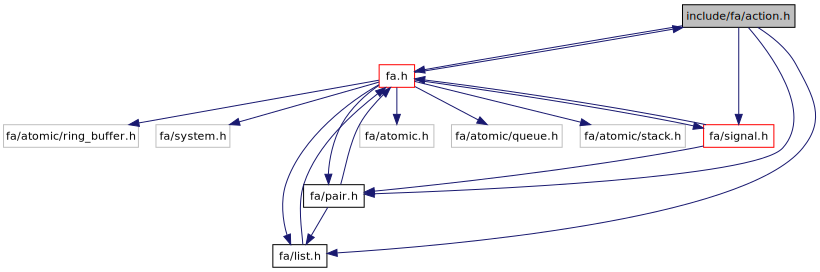
\includegraphics[width=350pt]{action_8h__incl}
\end{center}
\end{figure}
This graph shows which files directly or indirectly include this file\-:\nopagebreak
\begin{figure}[H]
\begin{center}
\leavevmode
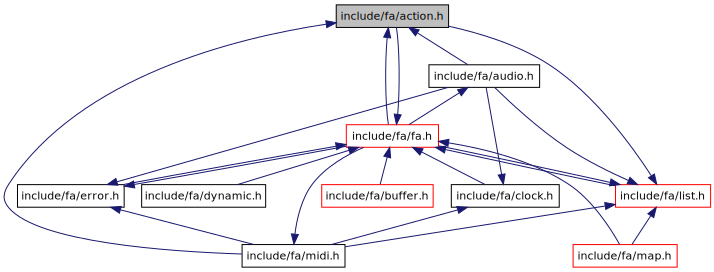
\includegraphics[width=350pt]{action_8h__dep__incl}
\end{center}
\end{figure}
\subsection*{Typedefs}
\begin{DoxyCompactItemize}
\item 
typedef struct \-\_\-fa\-\_\-action\-\_\-t $\ast$ \hyperlink{group___fa_action_gadb08ae063168671e5fedc6c23f20ae4b}{fa\-\_\-action\-\_\-t}
\begin{DoxyCompactList}\small\item\em The abstract type of actions. \end{DoxyCompactList}\item 
typedef int \hyperlink{group___fa_action_ga042610e7e8a7615937f5eeb3a8d789c5}{fa\-\_\-action\-\_\-channel\-\_\-t}
\begin{DoxyCompactList}\small\item\em Channel on which to carry out the action. \end{DoxyCompactList}\item 
typedef \hyperlink{group___fa_string_gacada63033b77bc6c39fa632ae199349b}{fa\-\_\-string\-\_\-t} \hyperlink{group___fa_action_ga44e517a8d2281a0556ac109c2b639d4b}{fa\-\_\-action\-\_\-name\-\_\-t}
\begin{DoxyCompactList}\small\item\em Name of external processor to receive the action. \end{DoxyCompactList}\item 
typedef \hyperlink{group___fa_ga915ddeae99ad7568b273d2b876425197}{fa\-\_\-ptr\-\_\-t} \hyperlink{group___fa_action_gaac4d474d26b235df5826124cb43464ce}{fa\-\_\-action\-\_\-value\-\_\-t}
\begin{DoxyCompactList}\small\item\em Value to send. \end{DoxyCompactList}\end{DoxyCompactItemize}
\subsection*{Functions}
\begin{DoxyCompactItemize}
\item 
\hyperlink{group___fa_action_gadb08ae063168671e5fedc6c23f20ae4b}{fa\-\_\-action\-\_\-t} \hyperlink{group___fa_action_ga94bd955f72ccc7f9ca6d5f7692cac4b9}{fa\-\_\-action\-\_\-null} ()
\begin{DoxyCompactList}\small\item\em The {\ttfamily null} action that does nothing. \end{DoxyCompactList}\item 
\hyperlink{group___fa_action_gadb08ae063168671e5fedc6c23f20ae4b}{fa\-\_\-action\-\_\-t} \hyperlink{group___fa_action_ga91980a1205ebea92b42647d78347edc7}{fa\-\_\-action\-\_\-copy} (\hyperlink{group___fa_action_gadb08ae063168671e5fedc6c23f20ae4b}{fa\-\_\-action\-\_\-t} action)
\begin{DoxyCompactList}\small\item\em Copy the given action. \end{DoxyCompactList}\item 
void \hyperlink{group___fa_action_ga43f9d05194a02cf4ea671342783be64a}{fa\-\_\-action\-\_\-destroy} (\hyperlink{group___fa_action_gadb08ae063168671e5fedc6c23f20ae4b}{fa\-\_\-action\-\_\-t} action)
\begin{DoxyCompactList}\small\item\em Destroy the given action. \end{DoxyCompactList}\item 
\hyperlink{group___fa_action_gadb08ae063168671e5fedc6c23f20ae4b}{fa\-\_\-action\-\_\-t} \hyperlink{group___fa_action_ga581ee60177355c84edb8bb919d4a4170}{fa\-\_\-action\-\_\-set} (\hyperlink{group___fa_action_ga042610e7e8a7615937f5eeb3a8d789c5}{fa\-\_\-action\-\_\-channel\-\_\-t} channel, double double\-\_\-)
\begin{DoxyCompactList}\small\item\em The {\ttfamily set} action updates a single global bus. \end{DoxyCompactList}\item 
\hyperlink{group___fa_action_gadb08ae063168671e5fedc6c23f20ae4b}{fa\-\_\-action\-\_\-t} \hyperlink{group___fa_action_ga6f5d14e19e9042a46f751659b0672285}{fa\-\_\-action\-\_\-accum} (\hyperlink{group___fa_action_ga042610e7e8a7615937f5eeb3a8d789c5}{fa\-\_\-action\-\_\-channel\-\_\-t} channel, \hyperlink{group___fa_signal_gaced7eb8d67eb2fe39927934c4abc7255}{fa\-\_\-signal\-\_\-unary\-\_\-double\-\_\-t} unary\-Double, \hyperlink{group___fa_ga915ddeae99ad7568b273d2b876425197}{fa\-\_\-ptr\-\_\-t} ptr)
\begin{DoxyCompactList}\small\item\em The {\ttfamily accum} action updates a single global bus by applying a function to its previous value. \end{DoxyCompactList}\item 
\hyperlink{group___fa_action_gadb08ae063168671e5fedc6c23f20ae4b}{fa\-\_\-action\-\_\-t} \hyperlink{group___fa_action_ga9f880ad4c24c7b3b897e5787ccaf0798}{fa\-\_\-action\-\_\-send} (\hyperlink{group___fa_action_ga44e517a8d2281a0556ac109c2b639d4b}{fa\-\_\-action\-\_\-name\-\_\-t} name, \hyperlink{group___fa_action_gaac4d474d26b235df5826124cb43464ce}{fa\-\_\-action\-\_\-value\-\_\-t} value)
\begin{DoxyCompactList}\small\item\em The {\ttfamily send} action sends a message, the type of which depends on the type of receiver. \end{DoxyCompactList}\item 
bool \hyperlink{group___fa_action_gafa9061ff63aaadf5078eccd7b534c139}{fa\-\_\-action\-\_\-is\-\_\-set} (\hyperlink{group___fa_action_gadb08ae063168671e5fedc6c23f20ae4b}{fa\-\_\-action\-\_\-t} action)
\begin{DoxyCompactList}\small\item\em Return whether the given action is a set action. \end{DoxyCompactList}\item 
\hyperlink{group___fa_action_ga042610e7e8a7615937f5eeb3a8d789c5}{fa\-\_\-action\-\_\-channel\-\_\-t} \hyperlink{group___fa_action_ga720fb58dfba134736c94d44aa441b59e}{fa\-\_\-action\-\_\-set\-\_\-channel} (\hyperlink{group___fa_action_gadb08ae063168671e5fedc6c23f20ae4b}{fa\-\_\-action\-\_\-t} action)
\begin{DoxyCompactList}\small\item\em Get the channel of a set action. \end{DoxyCompactList}\item 
double \hyperlink{group___fa_action_ga428cbdc66641d4404957b34b2b6789b0}{fa\-\_\-action\-\_\-set\-\_\-value} (\hyperlink{group___fa_action_gadb08ae063168671e5fedc6c23f20ae4b}{fa\-\_\-action\-\_\-t} action)
\begin{DoxyCompactList}\small\item\em Get the value of a set action. \end{DoxyCompactList}\item 
bool \hyperlink{group___fa_action_ga15e38e47b12339f92906e2c16ed65c2f}{fa\-\_\-action\-\_\-is\-\_\-accum} (\hyperlink{group___fa_action_gadb08ae063168671e5fedc6c23f20ae4b}{fa\-\_\-action\-\_\-t} action)
\begin{DoxyCompactList}\small\item\em Return whether the given action is an accumulation action. \end{DoxyCompactList}\item 
\hyperlink{group___fa_action_ga042610e7e8a7615937f5eeb3a8d789c5}{fa\-\_\-action\-\_\-channel\-\_\-t} \hyperlink{group___fa_action_ga90c8d6c961998de33f86ef37cc87d302}{fa\-\_\-action\-\_\-accum\-\_\-channel} (\hyperlink{group___fa_action_gadb08ae063168671e5fedc6c23f20ae4b}{fa\-\_\-action\-\_\-t} action)
\begin{DoxyCompactList}\small\item\em Get the channel of an accumulation action. \end{DoxyCompactList}\item 
\hyperlink{group___fa_signal_gaced7eb8d67eb2fe39927934c4abc7255}{fa\-\_\-signal\-\_\-unary\-\_\-double\-\_\-t} \hyperlink{group___fa_action_ga3b28dc4eb7ecaade47a508fa8844bcdb}{fa\-\_\-action\-\_\-accum\-\_\-function} (\hyperlink{group___fa_action_gadb08ae063168671e5fedc6c23f20ae4b}{fa\-\_\-action\-\_\-t} action)
\begin{DoxyCompactList}\small\item\em Get the function of an accumulation action. \end{DoxyCompactList}\item 
\hyperlink{group___fa_ga915ddeae99ad7568b273d2b876425197}{fa\-\_\-ptr\-\_\-t} \hyperlink{group___fa_action_ga0ef7b3178ab057a2d6b64472b866ab9c}{fa\-\_\-action\-\_\-accum\-\_\-data} (\hyperlink{group___fa_action_gadb08ae063168671e5fedc6c23f20ae4b}{fa\-\_\-action\-\_\-t} action)
\begin{DoxyCompactList}\small\item\em Get the data of an accumulation action. \end{DoxyCompactList}\item 
bool \hyperlink{group___fa_action_gacbe7fa1169a98d0c118845e79a48acd9}{fa\-\_\-action\-\_\-is\-\_\-send} (\hyperlink{group___fa_action_gadb08ae063168671e5fedc6c23f20ae4b}{fa\-\_\-action\-\_\-t} action)
\begin{DoxyCompactList}\small\item\em Return whether the given action is a send action. \end{DoxyCompactList}\item 
\hyperlink{group___fa_action_ga44e517a8d2281a0556ac109c2b639d4b}{fa\-\_\-action\-\_\-name\-\_\-t} \hyperlink{group___fa_action_ga061500ae01495bc9cec4c2c58973fcfd}{fa\-\_\-action\-\_\-send\-\_\-name} (\hyperlink{group___fa_action_gadb08ae063168671e5fedc6c23f20ae4b}{fa\-\_\-action\-\_\-t} action)
\begin{DoxyCompactList}\small\item\em Get the name of an send action. \end{DoxyCompactList}\item 
\hyperlink{group___fa_action_gaac4d474d26b235df5826124cb43464ce}{fa\-\_\-action\-\_\-value\-\_\-t} \hyperlink{group___fa_action_ga986a52955699094b178f850b92cb8bf0}{fa\-\_\-action\-\_\-send\-\_\-value} (\hyperlink{group___fa_action_gadb08ae063168671e5fedc6c23f20ae4b}{fa\-\_\-action\-\_\-t} action)
\begin{DoxyCompactList}\small\item\em Get the value of an send action. \end{DoxyCompactList}\item 
\hyperlink{group___fa_action_gadb08ae063168671e5fedc6c23f20ae4b}{fa\-\_\-action\-\_\-t} \hyperlink{group___fa_action_ga6e81ed66fec37b463601b62909051d6d}{fa\-\_\-action\-\_\-repeat} (\hyperlink{group___fa_time_ga227cc693f20b4873fed11028bcade184}{fa\-\_\-time\-\_\-t} interval, \hyperlink{group___fa_action_gadb08ae063168671e5fedc6c23f20ae4b}{fa\-\_\-action\-\_\-t} action)
\begin{DoxyCompactList}\small\item\em Repeat the given action indefinitely. \end{DoxyCompactList}\item 
\hyperlink{group___fa_action_gadb08ae063168671e5fedc6c23f20ae4b}{fa\-\_\-action\-\_\-t} \hyperlink{group___fa_action_ga9cd15b8d36f69d4ccb4e278a6cd97a32}{fa\-\_\-action\-\_\-many} (\hyperlink{group___fa_list_ga35ecb12ab934ded0cce0bcf28e3bc5d2}{fa\-\_\-list\-\_\-t} actions)
\begin{DoxyCompactList}\small\item\em Join a list of actions into a single compond action. \end{DoxyCompactList}\item 
\hyperlink{group___fa_action_gadb08ae063168671e5fedc6c23f20ae4b}{fa\-\_\-action\-\_\-t} \hyperlink{group___fa_action_ga90164c782d5a2a1e94cebd8828f36ea3}{fa\-\_\-action\-\_\-if} (\hyperlink{group___fa_gae6b6ae9fb073db0ba0bd323d511c6a98}{fa\-\_\-pred\-\_\-t} pred, \hyperlink{group___fa_ga915ddeae99ad7568b273d2b876425197}{fa\-\_\-ptr\-\_\-t} pred\-Data, \hyperlink{group___fa_action_gadb08ae063168671e5fedc6c23f20ae4b}{fa\-\_\-action\-\_\-t} action)
\begin{DoxyCompactList}\small\item\em Creates a derived action from the given action that executes íf and only given predicate holds. \end{DoxyCompactList}\item 
\hyperlink{group___fa_action_gadb08ae063168671e5fedc6c23f20ae4b}{fa\-\_\-action\-\_\-t} \hyperlink{group___fa_action_ga672d8e5edd644f5717ad4e3c3d61c382}{fa\-\_\-action\-\_\-while} (\hyperlink{group___fa_gae6b6ae9fb073db0ba0bd323d511c6a98}{fa\-\_\-pred\-\_\-t} pred, \hyperlink{group___fa_ga915ddeae99ad7568b273d2b876425197}{fa\-\_\-ptr\-\_\-t} pred\-Data, \hyperlink{group___fa_action_gadb08ae063168671e5fedc6c23f20ae4b}{fa\-\_\-action\-\_\-t} action)
\begin{DoxyCompactList}\small\item\em Creates a derived action from the given action that executes as long as the given predicate holds. \end{DoxyCompactList}\item 
\hyperlink{group___fa_action_gadb08ae063168671e5fedc6c23f20ae4b}{fa\-\_\-action\-\_\-t} \hyperlink{group___fa_action_ga738040c72d7251a5e1548cc94e3ab1b4}{fa\-\_\-action\-\_\-until} (\hyperlink{group___fa_gae6b6ae9fb073db0ba0bd323d511c6a98}{fa\-\_\-pred\-\_\-t} pred, \hyperlink{group___fa_ga915ddeae99ad7568b273d2b876425197}{fa\-\_\-ptr\-\_\-t} pred\-Data, \hyperlink{group___fa_action_gadb08ae063168671e5fedc6c23f20ae4b}{fa\-\_\-action\-\_\-t} action)
\begin{DoxyCompactList}\small\item\em Creates a derived action from the given action that executes as long as the given predicate does {\itshape not} hold. \end{DoxyCompactList}\item 
\hyperlink{group___fa_action_gadb08ae063168671e5fedc6c23f20ae4b}{fa\-\_\-action\-\_\-t} \hyperlink{group___fa_action_ga31bc40c290b44b342599fa0e1b8e2aa4}{fa\-\_\-action\-\_\-do} (\hyperlink{group___fa_ga43b940a9294fd58a54087ef0b416e479}{fa\-\_\-nullary\-\_\-t} nullary, \hyperlink{group___fa_ga915ddeae99ad7568b273d2b876425197}{fa\-\_\-ptr\-\_\-t} ptr)
\begin{DoxyCompactList}\small\item\em Convert a unary function to an action. \end{DoxyCompactList}\item 
bool \hyperlink{group___fa_action_ga434510734518ad00130c2e3a3ff61e50}{fa\-\_\-action\-\_\-is\-\_\-simple} (\hyperlink{group___fa_action_gadb08ae063168671e5fedc6c23f20ae4b}{fa\-\_\-action\-\_\-t} action)
\begin{DoxyCompactList}\small\item\em Returns whether the given action is simple or not. \end{DoxyCompactList}\item 
bool \hyperlink{group___fa_action_ga20bae4d808d585cd087f7c3e55afbc0e}{fa\-\_\-action\-\_\-is\-\_\-compound} (\hyperlink{group___fa_action_gadb08ae063168671e5fedc6c23f20ae4b}{fa\-\_\-action\-\_\-t} action)
\begin{DoxyCompactList}\small\item\em Returns whether the given action is compound or not. \end{DoxyCompactList}\item 
\hyperlink{group___fa_time_ga227cc693f20b4873fed11028bcade184}{fa\-\_\-time\-\_\-t} \hyperlink{group___fa_action_gae40a7127067b85b0d72e17dea130b613}{fa\-\_\-action\-\_\-compound\-\_\-interval} (\hyperlink{group___fa_action_gadb08ae063168671e5fedc6c23f20ae4b}{fa\-\_\-action\-\_\-t} action)
\begin{DoxyCompactList}\small\item\em Given a compound action, return the minimum offset to its tail. \end{DoxyCompactList}\item 
\hyperlink{group___fa_action_gadb08ae063168671e5fedc6c23f20ae4b}{fa\-\_\-action\-\_\-t} \hyperlink{group___fa_action_ga9f3ee907773b33a7a9eea5c6d083db3b}{fa\-\_\-action\-\_\-compound\-\_\-first} (\hyperlink{group___fa_action_gadb08ae063168671e5fedc6c23f20ae4b}{fa\-\_\-action\-\_\-t} action)
\begin{DoxyCompactList}\small\item\em Given a compound action, return its head (nullable). \end{DoxyCompactList}\item 
\hyperlink{group___fa_action_gadb08ae063168671e5fedc6c23f20ae4b}{fa\-\_\-action\-\_\-t} \hyperlink{group___fa_action_ga0aa70790832784b192117ec043b34b57}{fa\-\_\-action\-\_\-compound\-\_\-rest} (\hyperlink{group___fa_action_gadb08ae063168671e5fedc6c23f20ae4b}{fa\-\_\-action\-\_\-t} action)
\begin{DoxyCompactList}\small\item\em Given a compound action, return its tail (nullable). \end{DoxyCompactList}\end{DoxyCompactItemize}

\hypertarget{alloc_8h}{\section{include/fa/alloc.h File Reference}
\label{alloc_8h}\index{include/fa/alloc.\-h@{include/fa/alloc.\-h}}
}
This graph shows which files directly or indirectly include this file\-:\nopagebreak
\begin{figure}[H]
\begin{center}
\leavevmode
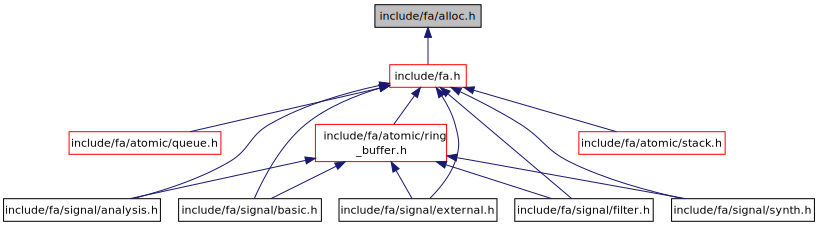
\includegraphics[width=350pt]{alloc_8h__dep__incl}
\end{center}
\end{figure}
\subsection*{Macros}
\begin{DoxyCompactItemize}
\item 
\#define \hyperlink{alloc_8h_af4254c22897cd7ec31ac52d20fd808ae}{fa\-\_\-new}(T)~\hyperlink{alloc_8h_af5ed0edc2b381ab04d1f6f8e0e18f933}{fa\-\_\-malloc}(sizeof(struct \-\_\-fa\-\_\-\#\#T\#\#\-\_\-t))
\item 
\#define \hyperlink{alloc_8h_ad61e673720215fcccb9dc57902e8fde4}{fa\-\_\-new\-\_\-struct}(T)~\hyperlink{alloc_8h_af5ed0edc2b381ab04d1f6f8e0e18f933}{fa\-\_\-malloc}(sizeof(struct T))
\item 
\#define \hyperlink{alloc_8h_af0ac57121ac73b73d732f425f589031f}{fa\-\_\-delete}(x)~\hyperlink{alloc_8h_afd68511245d1cc12f07d6249e6a8ce1e}{fa\-\_\-free}(x)
\end{DoxyCompactItemize}
\subsection*{Functions}
\begin{DoxyCompactItemize}
\item 
void $\ast$ \hyperlink{alloc_8h_af5ed0edc2b381ab04d1f6f8e0e18f933}{fa\-\_\-malloc} (size\-\_\-t size)
\item 
void $\ast$ \hyperlink{alloc_8h_ab1850d348d50dd021f200b6ac7c17617}{fa\-\_\-realloc} (void $\ast$ptr, size\-\_\-t size)
\item 
void \hyperlink{alloc_8h_afd68511245d1cc12f07d6249e6a8ce1e}{fa\-\_\-free} (void $\ast$ptr)
\end{DoxyCompactItemize}


\subsection{Macro Definition Documentation}
\hypertarget{alloc_8h_af4254c22897cd7ec31ac52d20fd808ae}{\index{alloc.\-h@{alloc.\-h}!fa\-\_\-new@{fa\-\_\-new}}
\index{fa\-\_\-new@{fa\-\_\-new}!alloc.h@{alloc.\-h}}
\subsubsection[{fa\-\_\-new}]{\setlength{\rightskip}{0pt plus 5cm}\#define fa\-\_\-new(
\begin{DoxyParamCaption}
\item[{}]{T}
\end{DoxyParamCaption}
)~{\bf fa\-\_\-malloc}(sizeof(struct \-\_\-fa\-\_\-\#\#T\#\#\-\_\-t))}}\label{alloc_8h_af4254c22897cd7ec31ac52d20fd808ae}
\hypertarget{alloc_8h_ad61e673720215fcccb9dc57902e8fde4}{\index{alloc.\-h@{alloc.\-h}!fa\-\_\-new\-\_\-struct@{fa\-\_\-new\-\_\-struct}}
\index{fa\-\_\-new\-\_\-struct@{fa\-\_\-new\-\_\-struct}!alloc.h@{alloc.\-h}}
\subsubsection[{fa\-\_\-new\-\_\-struct}]{\setlength{\rightskip}{0pt plus 5cm}\#define fa\-\_\-new\-\_\-struct(
\begin{DoxyParamCaption}
\item[{}]{T}
\end{DoxyParamCaption}
)~{\bf fa\-\_\-malloc}(sizeof(struct T))}}\label{alloc_8h_ad61e673720215fcccb9dc57902e8fde4}
\hypertarget{alloc_8h_af0ac57121ac73b73d732f425f589031f}{\index{alloc.\-h@{alloc.\-h}!fa\-\_\-delete@{fa\-\_\-delete}}
\index{fa\-\_\-delete@{fa\-\_\-delete}!alloc.h@{alloc.\-h}}
\subsubsection[{fa\-\_\-delete}]{\setlength{\rightskip}{0pt plus 5cm}\#define fa\-\_\-delete(
\begin{DoxyParamCaption}
\item[{}]{x}
\end{DoxyParamCaption}
)~{\bf fa\-\_\-free}(x)}}\label{alloc_8h_af0ac57121ac73b73d732f425f589031f}


\subsection{Function Documentation}
\hypertarget{alloc_8h_af5ed0edc2b381ab04d1f6f8e0e18f933}{\index{alloc.\-h@{alloc.\-h}!fa\-\_\-malloc@{fa\-\_\-malloc}}
\index{fa\-\_\-malloc@{fa\-\_\-malloc}!alloc.h@{alloc.\-h}}
\subsubsection[{fa\-\_\-malloc}]{\setlength{\rightskip}{0pt plus 5cm}void$\ast$ fa\-\_\-malloc (
\begin{DoxyParamCaption}
\item[{size\-\_\-t}]{size}
\end{DoxyParamCaption}
)}}\label{alloc_8h_af5ed0edc2b381ab04d1f6f8e0e18f933}
\hypertarget{alloc_8h_ab1850d348d50dd021f200b6ac7c17617}{\index{alloc.\-h@{alloc.\-h}!fa\-\_\-realloc@{fa\-\_\-realloc}}
\index{fa\-\_\-realloc@{fa\-\_\-realloc}!alloc.h@{alloc.\-h}}
\subsubsection[{fa\-\_\-realloc}]{\setlength{\rightskip}{0pt plus 5cm}void$\ast$ fa\-\_\-realloc (
\begin{DoxyParamCaption}
\item[{void $\ast$}]{ptr, }
\item[{size\-\_\-t}]{size}
\end{DoxyParamCaption}
)}}\label{alloc_8h_ab1850d348d50dd021f200b6ac7c17617}
\hypertarget{alloc_8h_afd68511245d1cc12f07d6249e6a8ce1e}{\index{alloc.\-h@{alloc.\-h}!fa\-\_\-free@{fa\-\_\-free}}
\index{fa\-\_\-free@{fa\-\_\-free}!alloc.h@{alloc.\-h}}
\subsubsection[{fa\-\_\-free}]{\setlength{\rightskip}{0pt plus 5cm}void fa\-\_\-free (
\begin{DoxyParamCaption}
\item[{void $\ast$}]{ptr}
\end{DoxyParamCaption}
)}}\label{alloc_8h_afd68511245d1cc12f07d6249e6a8ce1e}

\hypertarget{atomic_8h}{\section{include/fa/atomic.h File Reference}
\label{atomic_8h}\index{include/fa/atomic.\-h@{include/fa/atomic.\-h}}
}
{\ttfamily \#include $<$fa.\-h$>$}\\*
{\ttfamily \#include $<$fa/std.\-h$>$}\\*
Include dependency graph for atomic.\-h\-:\nopagebreak
\begin{figure}[H]
\begin{center}
\leavevmode
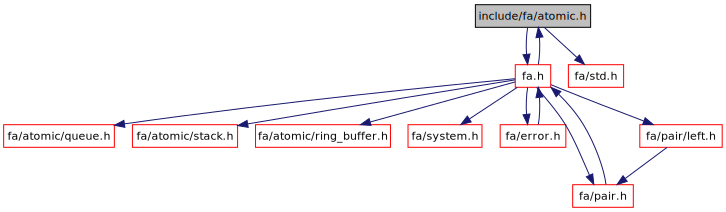
\includegraphics[width=350pt]{atomic_8h__incl}
\end{center}
\end{figure}
This graph shows which files directly or indirectly include this file\-:\nopagebreak
\begin{figure}[H]
\begin{center}
\leavevmode
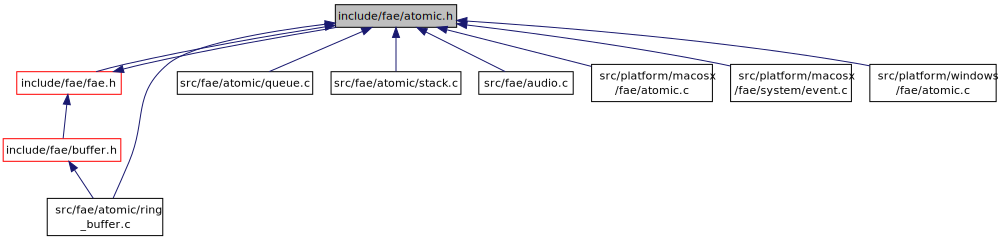
\includegraphics[width=350pt]{atomic_8h__dep__incl}
\end{center}
\end{figure}
\subsection*{Typedefs}
\begin{DoxyCompactItemize}
\item 
typedef struct \-\_\-fa\-\_\-atomic\-\_\-t $\ast$ \hyperlink{group___fa_atomic_gaa3c9a8cdc36169052d96fa152e2eb9ae}{fa\-\_\-atomic\-\_\-t}
\end{DoxyCompactItemize}
\subsection*{Functions}
\begin{DoxyCompactItemize}
\item 
\hyperlink{group___fa_atomic_gaa3c9a8cdc36169052d96fa152e2eb9ae}{fa\-\_\-atomic\-\_\-t} \hyperlink{group___fa_atomic_ga4342c7467122777598bda9c4fbe55b8d}{fa\-\_\-atomic\-\_\-create} ()
\begin{DoxyCompactList}\small\item\em Create a new atomic reference. \end{DoxyCompactList}\item 
\hyperlink{group___fa_atomic_gaa3c9a8cdc36169052d96fa152e2eb9ae}{fa\-\_\-atomic\-\_\-t} \hyperlink{group___fa_atomic_ga202aa48a1cdf0904cc124c7a79c49396}{fa\-\_\-atomic\-\_\-copy} (\hyperlink{group___fa_atomic_gaa3c9a8cdc36169052d96fa152e2eb9ae}{fa\-\_\-atomic\-\_\-t} \hyperlink{util_8h_a5181e62dd55d17e3c1fd4ad40865f737}{atomic})
\begin{DoxyCompactList}\small\item\em Copy the given atomic reference. \end{DoxyCompactList}\item 
void \hyperlink{group___fa_atomic_gafd51f6eb1c2815d3f7cd6d571be2f3da}{fa\-\_\-atomic\-\_\-destroy} (\hyperlink{group___fa_atomic_gaa3c9a8cdc36169052d96fa152e2eb9ae}{fa\-\_\-atomic\-\_\-t} \hyperlink{util_8h_a5181e62dd55d17e3c1fd4ad40865f737}{atomic})
\begin{DoxyCompactList}\small\item\em Destroy the given atomic reference. \end{DoxyCompactList}\item 
bool \hyperlink{group___fa_atomic_ga3a965277fde384ba27a422cb80fda193}{fa\-\_\-atomic\-\_\-exchange} (\hyperlink{group___fa_atomic_gaa3c9a8cdc36169052d96fa152e2eb9ae}{fa\-\_\-atomic\-\_\-t} \hyperlink{util_8h_a5181e62dd55d17e3c1fd4ad40865f737}{atomic}, \hyperlink{group___fa_ga915ddeae99ad7568b273d2b876425197}{fa\-\_\-ptr\-\_\-t} ptr, \hyperlink{group___fa_ga915ddeae99ad7568b273d2b876425197}{fa\-\_\-ptr\-\_\-t} ptr\-\_\-)
\begin{DoxyCompactList}\small\item\em Compares the given value with the current value of the given atomic reference, replacing it if successful. \end{DoxyCompactList}\item 
\hyperlink{group___fa_ga915ddeae99ad7568b273d2b876425197}{fa\-\_\-ptr\-\_\-t} \hyperlink{group___fa_atomic_gae9136728ae2e5c0f75c29c5a262c510a}{fa\-\_\-atomic\-\_\-get} (\hyperlink{group___fa_atomic_gaa3c9a8cdc36169052d96fa152e2eb9ae}{fa\-\_\-atomic\-\_\-t} \hyperlink{util_8h_a5181e62dd55d17e3c1fd4ad40865f737}{atomic})
\begin{DoxyCompactList}\small\item\em Return the current value of the given atomic reference. \end{DoxyCompactList}\item 
void \hyperlink{group___fa_atomic_ga4bc5dbae5b252ac051f62e693f6def76}{fa\-\_\-atomic\-\_\-modify} (\hyperlink{group___fa_atomic_gaa3c9a8cdc36169052d96fa152e2eb9ae}{fa\-\_\-atomic\-\_\-t} \hyperlink{util_8h_a5181e62dd55d17e3c1fd4ad40865f737}{atomic}, \hyperlink{group___fa_gaaafae8ab9ebae9019133108e56d2d4d1}{fa\-\_\-unary\-\_\-t} unary, \hyperlink{group___fa_ga915ddeae99ad7568b273d2b876425197}{fa\-\_\-ptr\-\_\-t} ptr)
\begin{DoxyCompactList}\small\item\em Update the given atomic value by applying the given pure function. \end{DoxyCompactList}\item 
void \hyperlink{group___fa_atomic_ga7730f096607dfd90b6af08d70fe1c9c7}{fa\-\_\-atomic\-\_\-set} (\hyperlink{group___fa_atomic_gaa3c9a8cdc36169052d96fa152e2eb9ae}{fa\-\_\-atomic\-\_\-t} \hyperlink{util_8h_a5181e62dd55d17e3c1fd4ad40865f737}{atomic}, \hyperlink{group___fa_ga915ddeae99ad7568b273d2b876425197}{fa\-\_\-ptr\-\_\-t} ptr)
\begin{DoxyCompactList}\small\item\em Set the given given atomic reference. \end{DoxyCompactList}\end{DoxyCompactItemize}

\hypertarget{queue_8h}{\section{include/fa/atomic/queue.h File Reference}
\label{queue_8h}\index{include/fa/atomic/queue.\-h@{include/fa/atomic/queue.\-h}}
}
{\ttfamily \#include $<$fa.\-h$>$}\\*
Include dependency graph for queue.\-h\-:\nopagebreak
\begin{figure}[H]
\begin{center}
\leavevmode
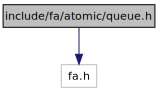
\includegraphics[width=230pt]{queue_8h__incl}
\end{center}
\end{figure}
This graph shows which files directly or indirectly include this file\-:\nopagebreak
\begin{figure}[H]
\begin{center}
\leavevmode
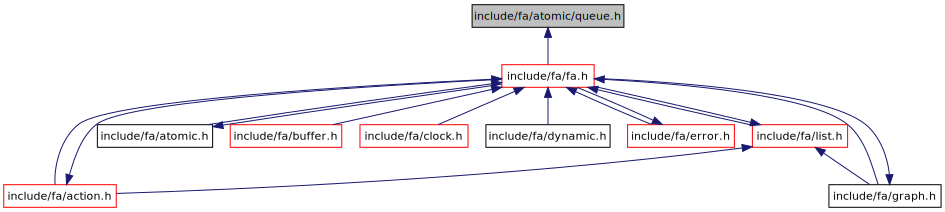
\includegraphics[width=350pt]{queue_8h__dep__incl}
\end{center}
\end{figure}
\subsection*{Typedefs}
\begin{DoxyCompactItemize}
\item 
typedef struct \-\_\-fa\-\_\-atomic\-\_\-queue\-\_\-t $\ast$ \hyperlink{group___fa_atomic_queue_ga31bf61a25a3ef94a5590f863b5448be7}{fa\-\_\-atomic\-\_\-queue\-\_\-t}
\end{DoxyCompactItemize}
\subsection*{Functions}
\begin{DoxyCompactItemize}
\item 
\hyperlink{group___fa_atomic_queue_ga31bf61a25a3ef94a5590f863b5448be7}{fa\-\_\-atomic\-\_\-queue\-\_\-t} \hyperlink{group___fa_atomic_queue_gab64418bd1d44abd7e744450c27013381}{fa\-\_\-atomic\-\_\-queue\-\_\-create} ()
\begin{DoxyCompactList}\small\item\em Create a new queue. \end{DoxyCompactList}\item 
void \hyperlink{group___fa_atomic_queue_ga348fb67019a6c3548449db7f6fdc5497}{fa\-\_\-atomic\-\_\-queue\-\_\-destroy} (\hyperlink{group___fa_atomic_queue_ga31bf61a25a3ef94a5590f863b5448be7}{fa\-\_\-atomic\-\_\-queue\-\_\-t} queue)
\begin{DoxyCompactList}\small\item\em Destroy the given queue. \end{DoxyCompactList}\item 
\hyperlink{group___fa_ga915ddeae99ad7568b273d2b876425197}{fa\-\_\-ptr\-\_\-t} \hyperlink{group___fa_atomic_queue_gab3d856bfd5a77e0fedf138e2c64eb239}{fa\-\_\-atomic\-\_\-queue\-\_\-read} (\hyperlink{group___fa_atomic_queue_ga31bf61a25a3ef94a5590f863b5448be7}{fa\-\_\-atomic\-\_\-queue\-\_\-t} queue)
\begin{DoxyCompactList}\small\item\em Read a value from the given queue. \end{DoxyCompactList}\item 
bool \hyperlink{group___fa_atomic_queue_ga0f28dbe53a428bafc02662c99d71b025}{fa\-\_\-atomic\-\_\-queue\-\_\-write} (\hyperlink{group___fa_atomic_queue_ga31bf61a25a3ef94a5590f863b5448be7}{fa\-\_\-atomic\-\_\-queue\-\_\-t} queue, \hyperlink{group___fa_ga915ddeae99ad7568b273d2b876425197}{fa\-\_\-ptr\-\_\-t} ptr)
\begin{DoxyCompactList}\small\item\em Write the given value to the given queue. \end{DoxyCompactList}\end{DoxyCompactItemize}

\hypertarget{ring__buffer_8h}{\section{include/fa/atomic/ring\-\_\-buffer.h File Reference}
\label{ring__buffer_8h}\index{include/fa/atomic/ring\-\_\-buffer.\-h@{include/fa/atomic/ring\-\_\-buffer.\-h}}
}
{\ttfamily \#include $<$fa.\-h$>$}\\*
Include dependency graph for ring\-\_\-buffer.\-h\-:\nopagebreak
\begin{figure}[H]
\begin{center}
\leavevmode
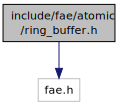
\includegraphics[width=210pt]{ring__buffer_8h__incl}
\end{center}
\end{figure}
This graph shows which files directly or indirectly include this file\-:\nopagebreak
\begin{figure}[H]
\begin{center}
\leavevmode
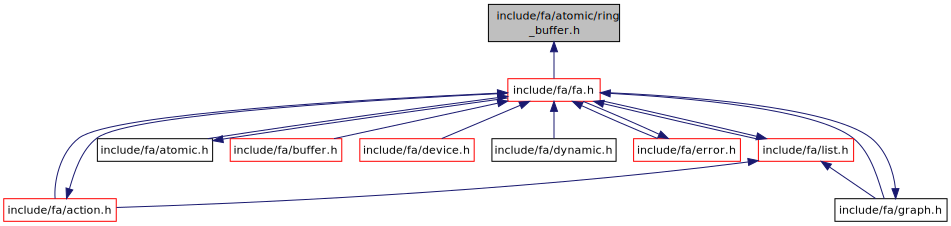
\includegraphics[width=350pt]{ring__buffer_8h__dep__incl}
\end{center}
\end{figure}
\subsection*{Typedefs}
\begin{DoxyCompactItemize}
\item 
typedef struct \\*
\-\_\-fa\-\_\-atomic\-\_\-ring\-\_\-buffer\-\_\-t $\ast$ \hyperlink{group___fa_atomic_ring_buffer_ga3482421740e66f489d94407a0d48a2d0}{fa\-\_\-atomic\-\_\-ring\-\_\-buffer\-\_\-t}
\end{DoxyCompactItemize}
\subsection*{Functions}
\begin{DoxyCompactItemize}
\item 
\hyperlink{group___fa_atomic_ring_buffer_ga3482421740e66f489d94407a0d48a2d0}{fa\-\_\-atomic\-\_\-ring\-\_\-buffer\-\_\-t} \hyperlink{group___fa_atomic_ring_buffer_ga6abb04c5ec0718605e4e24927047d4c7}{fa\-\_\-atomic\-\_\-ring\-\_\-buffer\-\_\-create} (size\-\_\-t size\-\_\-)
\item 
void \hyperlink{group___fa_atomic_ring_buffer_gaf49af6bcd11c9ebb4c6b8554aea829b8}{fa\-\_\-atomic\-\_\-ring\-\_\-buffer\-\_\-destroy} (\hyperlink{group___fa_atomic_ring_buffer_ga3482421740e66f489d94407a0d48a2d0}{fa\-\_\-atomic\-\_\-ring\-\_\-buffer\-\_\-t} ring\-Buffer)
\item 
size\-\_\-t \hyperlink{group___fa_atomic_ring_buffer_gae2ac670afafeff9b8150ae9649c83474}{fa\-\_\-atomic\-\_\-ring\-\_\-buffer\-\_\-size} (\hyperlink{group___fa_atomic_ring_buffer_ga3482421740e66f489d94407a0d48a2d0}{fa\-\_\-atomic\-\_\-ring\-\_\-buffer\-\_\-t} ring\-Buffer)
\item 
void \hyperlink{group___fa_atomic_ring_buffer_ga56faff64e32a993b750380571bfb8c76}{fa\-\_\-atomic\-\_\-ring\-\_\-buffer\-\_\-close} (\hyperlink{group___fa_atomic_ring_buffer_ga3482421740e66f489d94407a0d48a2d0}{fa\-\_\-atomic\-\_\-ring\-\_\-buffer\-\_\-t} ring\-Buffer)
\item 
bool \hyperlink{group___fa_atomic_ring_buffer_ga4fc04706251e284c9701b6ad95abf377}{fa\-\_\-atomic\-\_\-ring\-\_\-buffer\-\_\-is\-\_\-closed} (\hyperlink{group___fa_atomic_ring_buffer_ga3482421740e66f489d94407a0d48a2d0}{fa\-\_\-atomic\-\_\-ring\-\_\-buffer\-\_\-t} ring\-Buffer)
\item 
bool \hyperlink{group___fa_atomic_ring_buffer_gace79351690263650a000919845b2ca62}{fa\-\_\-atomic\-\_\-ring\-\_\-buffer\-\_\-can\-\_\-read} (\hyperlink{group___fa_atomic_ring_buffer_ga3482421740e66f489d94407a0d48a2d0}{fa\-\_\-atomic\-\_\-ring\-\_\-buffer\-\_\-t} ring\-Buffer, size\-\_\-t size\-\_\-)
\item 
bool \hyperlink{group___fa_atomic_ring_buffer_ga974e7b9a3dfb32ce44c58fbf6a25dc4f}{fa\-\_\-atomic\-\_\-ring\-\_\-buffer\-\_\-can\-\_\-write} (\hyperlink{group___fa_atomic_ring_buffer_ga3482421740e66f489d94407a0d48a2d0}{fa\-\_\-atomic\-\_\-ring\-\_\-buffer\-\_\-t} ring\-Buffer, size\-\_\-t size\-\_\-)
\item 
bool \hyperlink{group___fa_atomic_ring_buffer_ga0441ea58fc6c6ceeafc94a1e2bea972c}{fa\-\_\-atomic\-\_\-ring\-\_\-buffer\-\_\-read} (\hyperlink{group___fa_atomic_ring_buffer_ga3482421740e66f489d94407a0d48a2d0}{fa\-\_\-atomic\-\_\-ring\-\_\-buffer\-\_\-t} ring\-Buffer, uint8\-\_\-t $\ast$)
\item 
bool \hyperlink{group___fa_atomic_ring_buffer_ga82065e6a2a97af64680ff8baff425ee1}{fa\-\_\-atomic\-\_\-ring\-\_\-buffer\-\_\-read\-\_\-float} (\hyperlink{group___fa_atomic_ring_buffer_ga3482421740e66f489d94407a0d48a2d0}{fa\-\_\-atomic\-\_\-ring\-\_\-buffer\-\_\-t} ring\-Buffer, float $\ast$)
\item 
bool \hyperlink{group___fa_atomic_ring_buffer_ga1599406f0bb153334cd10ae90ab919f1}{fa\-\_\-atomic\-\_\-ring\-\_\-buffer\-\_\-read\-\_\-double} (\hyperlink{group___fa_atomic_ring_buffer_ga3482421740e66f489d94407a0d48a2d0}{fa\-\_\-atomic\-\_\-ring\-\_\-buffer\-\_\-t} ring\-Buffer, double $\ast$)
\item 
bool \hyperlink{group___fa_atomic_ring_buffer_ga18a7f61a001df0e2606280a9aead1ddf}{fa\-\_\-atomic\-\_\-ring\-\_\-buffer\-\_\-write} (\hyperlink{group___fa_atomic_ring_buffer_ga3482421740e66f489d94407a0d48a2d0}{fa\-\_\-atomic\-\_\-ring\-\_\-buffer\-\_\-t} ring\-Buffer, uint8\-\_\-t u\-Int8\-\_\-)
\item 
bool \hyperlink{group___fa_atomic_ring_buffer_gade9d350cfae7b805353a3b58b9d17a7e}{fa\-\_\-atomic\-\_\-ring\-\_\-buffer\-\_\-write\-\_\-float} (\hyperlink{group___fa_atomic_ring_buffer_ga3482421740e66f489d94407a0d48a2d0}{fa\-\_\-atomic\-\_\-ring\-\_\-buffer\-\_\-t} ring\-Buffer, float float\-\_\-)
\item 
bool \hyperlink{group___fa_atomic_ring_buffer_gafd68caebbb7b3f6e62f604a6e6915e90}{fa\-\_\-atomic\-\_\-ring\-\_\-buffer\-\_\-write\-\_\-double} (\hyperlink{group___fa_atomic_ring_buffer_ga3482421740e66f489d94407a0d48a2d0}{fa\-\_\-atomic\-\_\-ring\-\_\-buffer\-\_\-t} ring\-Buffer, double double\-\_\-)
\end{DoxyCompactItemize}

\hypertarget{stack_8h}{\section{include/fa/atomic/stack.h File Reference}
\label{stack_8h}\index{include/fa/atomic/stack.\-h@{include/fa/atomic/stack.\-h}}
}
{\ttfamily \#include $<$fa.\-h$>$}\\*
Include dependency graph for stack.\-h\-:\nopagebreak
\begin{figure}[H]
\begin{center}
\leavevmode
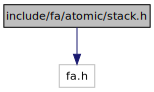
\includegraphics[width=226pt]{stack_8h__incl}
\end{center}
\end{figure}
This graph shows which files directly or indirectly include this file\-:\nopagebreak
\begin{figure}[H]
\begin{center}
\leavevmode
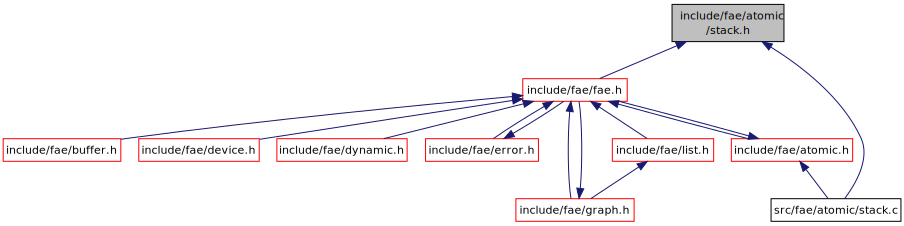
\includegraphics[width=350pt]{stack_8h__dep__incl}
\end{center}
\end{figure}
\subsection*{Typedefs}
\begin{DoxyCompactItemize}
\item 
typedef struct \-\_\-fa\-\_\-atomic\-\_\-stack\-\_\-t $\ast$ \hyperlink{group___fa_atomic_stack_ga12448e3a1d7002a702efc2a78eebfa69}{fa\-\_\-atomic\-\_\-stack\-\_\-t}
\end{DoxyCompactItemize}
\subsection*{Functions}
\begin{DoxyCompactItemize}
\item 
\hyperlink{group___fa_atomic_stack_ga12448e3a1d7002a702efc2a78eebfa69}{fa\-\_\-atomic\-\_\-stack\-\_\-t} \hyperlink{group___fa_atomic_stack_gacfb347f6def65c5207877d6dba9fbc62}{fa\-\_\-atomic\-\_\-stack\-\_\-create} ()
\begin{DoxyCompactList}\small\item\em Create a new stack. \end{DoxyCompactList}\item 
void \hyperlink{group___fa_atomic_stack_gafd7a22df157d016f336a304c311c0634}{fa\-\_\-atomic\-\_\-stack\-\_\-destroy} (\hyperlink{group___fa_atomic_stack_ga12448e3a1d7002a702efc2a78eebfa69}{fa\-\_\-atomic\-\_\-stack\-\_\-t} stack)
\begin{DoxyCompactList}\small\item\em Destroy the given stack. \end{DoxyCompactList}\item 
\hyperlink{group___fa_ga915ddeae99ad7568b273d2b876425197}{fa\-\_\-ptr\-\_\-t} \hyperlink{group___fa_atomic_stack_ga7d8023ec59ac028da1188064eff7f642}{fa\-\_\-atomic\-\_\-stack\-\_\-read} (\hyperlink{group___fa_atomic_stack_ga12448e3a1d7002a702efc2a78eebfa69}{fa\-\_\-atomic\-\_\-stack\-\_\-t} stack)
\begin{DoxyCompactList}\small\item\em Read a value from the given stack. \end{DoxyCompactList}\item 
bool \hyperlink{group___fa_atomic_stack_gae7220769ca5217af9935f3bde86fbf75}{fa\-\_\-atomic\-\_\-stack\-\_\-write} (\hyperlink{group___fa_atomic_stack_ga12448e3a1d7002a702efc2a78eebfa69}{fa\-\_\-atomic\-\_\-stack\-\_\-t} stack, \hyperlink{group___fa_ga915ddeae99ad7568b273d2b876425197}{fa\-\_\-ptr\-\_\-t} ptr)
\begin{DoxyCompactList}\small\item\em Write the given value to the given stack. \end{DoxyCompactList}\end{DoxyCompactItemize}

\hypertarget{audio_8h}{\section{include/fa/audio.h File Reference}
\label{audio_8h}\index{include/fa/audio.\-h@{include/fa/audio.\-h}}
}
{\ttfamily \#include $<$fa/audio/session.\-h$>$}\\*
{\ttfamily \#include $<$fa/audio/device.\-h$>$}\\*
{\ttfamily \#include $<$fa/audio/stream.\-h$>$}\\*
Include dependency graph for audio.\-h\-:\nopagebreak
\begin{figure}[H]
\begin{center}
\leavevmode
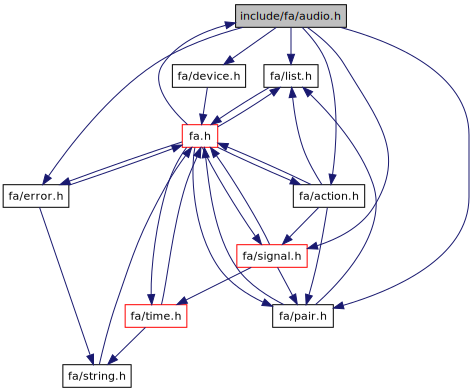
\includegraphics[width=350pt]{audio_8h__incl}
\end{center}
\end{figure}
This graph shows which files directly or indirectly include this file\-:\nopagebreak
\begin{figure}[H]
\begin{center}
\leavevmode
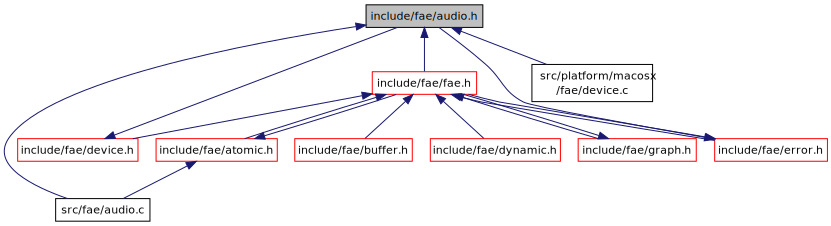
\includegraphics[width=350pt]{audio_8h__dep__incl}
\end{center}
\end{figure}

\hypertarget{audio_2device_8h}{\section{include/fa/audio/device.h File Reference}
\label{audio_2device_8h}\index{include/fa/audio/device.\-h@{include/fa/audio/device.\-h}}
}
{\ttfamily \#include $<$fa/action.\-h$>$}\\*
{\ttfamily \#include $<$fa/time.\-h$>$}\\*
{\ttfamily \#include $<$fa/clock.\-h$>$}\\*
{\ttfamily \#include $<$fa/audio/session.\-h$>$}\\*
Include dependency graph for device.\-h\-:\nopagebreak
\begin{figure}[H]
\begin{center}
\leavevmode
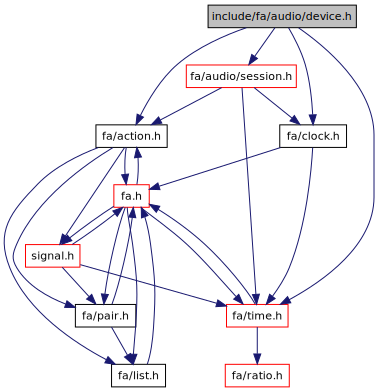
\includegraphics[width=350pt]{audio_2device_8h__incl}
\end{center}
\end{figure}
This graph shows which files directly or indirectly include this file\-:\nopagebreak
\begin{figure}[H]
\begin{center}
\leavevmode
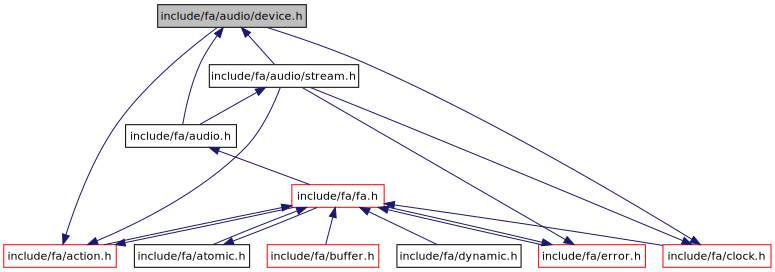
\includegraphics[width=350pt]{audio_2device_8h__dep__incl}
\end{center}
\end{figure}
\subsection*{Typedefs}
\begin{DoxyCompactItemize}
\item 
typedef struct \-\_\-fa\-\_\-audio\-\_\-device\-\_\-t $\ast$ \hyperlink{group___fa_audio_device_ga03de89ee66c6465f8cedd3a0286598f4}{fa\-\_\-audio\-\_\-device\-\_\-t}
\begin{DoxyCompactList}\small\item\em An audio device. \end{DoxyCompactList}\item 
typedef \hyperlink{group___fa_list_ga35ecb12ab934ded0cce0bcf28e3bc5d2}{fa\-\_\-list\-\_\-t}($\ast$ \hyperlink{group___fa_audio_device_gae190189bb20427f20453f2e4d48ecc7b}{fa\-\_\-audio\-\_\-proc\-\_\-t} )(\hyperlink{group___fa_ga915ddeae99ad7568b273d2b876425197}{fa\-\_\-ptr\-\_\-t}, \hyperlink{group___fa_list_ga35ecb12ab934ded0cce0bcf28e3bc5d2}{fa\-\_\-list\-\_\-t})
\begin{DoxyCompactList}\small\item\em An audio processor, or a function from a list of signals to a list of signals. \end{DoxyCompactList}\end{DoxyCompactItemize}
\subsection*{Functions}
\begin{DoxyCompactItemize}
\item 
\hyperlink{group___fa_pair_gac2b2e58c230bac4f8a63ef6c05072680}{fa\-\_\-pair\-\_\-t} \hyperlink{group___fa_audio_device_gab51159ac7fd84af31a985e96f4f9c20f}{fa\-\_\-audio\-\_\-default} (\hyperlink{group___fa_audio_session_ga62ee22268c23f1b18447141feccc01e0}{fa\-\_\-audio\-\_\-session\-\_\-t} session)
\begin{DoxyCompactList}\small\item\em Get the standard devices of the given session. \end{DoxyCompactList}\item 
\hyperlink{group___fa_audio_device_ga03de89ee66c6465f8cedd3a0286598f4}{fa\-\_\-audio\-\_\-device\-\_\-t} \hyperlink{group___fa_audio_device_ga690374b4ffcee314cb4cdad6309ef817}{fa\-\_\-audio\-\_\-default\-\_\-input} (\hyperlink{group___fa_audio_session_ga62ee22268c23f1b18447141feccc01e0}{fa\-\_\-audio\-\_\-session\-\_\-t} session)
\begin{DoxyCompactList}\small\item\em Get the standard input device of the given session. \end{DoxyCompactList}\item 
\hyperlink{group___fa_audio_device_ga03de89ee66c6465f8cedd3a0286598f4}{fa\-\_\-audio\-\_\-device\-\_\-t} \hyperlink{group___fa_audio_device_ga364583565c9405e541ae52e41efa38e7}{fa\-\_\-audio\-\_\-default\-\_\-output} (\hyperlink{group___fa_audio_session_ga62ee22268c23f1b18447141feccc01e0}{fa\-\_\-audio\-\_\-session\-\_\-t} session)
\begin{DoxyCompactList}\small\item\em Get the standard output device of the given session. \end{DoxyCompactList}\item 
void \hyperlink{group___fa_audio_device_ga53538690e8c1eeebb470b99306fe289d}{fa\-\_\-audio\-\_\-add\-\_\-status\-\_\-callback} (\hyperlink{group___fa_audio_session_gaac3fa018078a475e6c5ed48efcbdb887}{fa\-\_\-audio\-\_\-status\-\_\-callback\-\_\-t} status\-Callback, \hyperlink{group___fa_ga915ddeae99ad7568b273d2b876425197}{fa\-\_\-ptr\-\_\-t} ptr, \hyperlink{group___fa_audio_session_ga62ee22268c23f1b18447141feccc01e0}{fa\-\_\-audio\-\_\-session\-\_\-t} session)
\begin{DoxyCompactList}\small\item\em Register a callback to be invoked when a hardware change is detected. \end{DoxyCompactList}\item 
\hyperlink{group___fa_audio_session_ga62ee22268c23f1b18447141feccc01e0}{fa\-\_\-audio\-\_\-session\-\_\-t} \hyperlink{group___fa_audio_device_ga75ce8ffa723a549c4ea41b7ead4fcb9b}{fa\-\_\-audio\-\_\-session} (\hyperlink{group___fa_audio_device_ga03de89ee66c6465f8cedd3a0286598f4}{fa\-\_\-audio\-\_\-device\-\_\-t} device)
\begin{DoxyCompactList}\small\item\em Return the session associated with the given device. \end{DoxyCompactList}\item 
\hyperlink{group___fa_string_gacada63033b77bc6c39fa632ae199349b}{fa\-\_\-string\-\_\-t} \hyperlink{group___fa_audio_device_ga8e04c8feea7e664d2c7de9c9e57a5f4e}{fa\-\_\-audio\-\_\-name} (\hyperlink{group___fa_audio_device_ga03de89ee66c6465f8cedd3a0286598f4}{fa\-\_\-audio\-\_\-device\-\_\-t} device)
\begin{DoxyCompactList}\small\item\em Return the name of the given device. \end{DoxyCompactList}\item 
\hyperlink{group___fa_string_gacada63033b77bc6c39fa632ae199349b}{fa\-\_\-string\-\_\-t} \hyperlink{group___fa_audio_device_ga3263e679dfa30fcd21042528782507d8}{fa\-\_\-audio\-\_\-host\-\_\-name} (\hyperlink{group___fa_audio_device_ga03de89ee66c6465f8cedd3a0286598f4}{fa\-\_\-audio\-\_\-device\-\_\-t} device)
\begin{DoxyCompactList}\small\item\em Return the host name of the given device. \end{DoxyCompactList}\item 
bool \hyperlink{group___fa_audio_device_gacd32b5e58c2b79df883a64d4012302ae}{fa\-\_\-audio\-\_\-has\-\_\-input} (\hyperlink{group___fa_audio_device_ga03de89ee66c6465f8cedd3a0286598f4}{fa\-\_\-audio\-\_\-device\-\_\-t} device)
\begin{DoxyCompactList}\small\item\em Return whether the given device has input or not. \end{DoxyCompactList}\item 
bool \hyperlink{group___fa_audio_device_ga2ca67bc0e45609675bb064849d20dba6}{fa\-\_\-audio\-\_\-has\-\_\-output} (\hyperlink{group___fa_audio_device_ga03de89ee66c6465f8cedd3a0286598f4}{fa\-\_\-audio\-\_\-device\-\_\-t} device)
\begin{DoxyCompactList}\small\item\em Return whether the given device has output or not. \end{DoxyCompactList}\item 
int \hyperlink{group___fa_audio_device_ga459971e7fd609eb0bb9f7ac0fffc156b}{fa\-\_\-audio\-\_\-input\-\_\-channels} (\hyperlink{group___fa_audio_device_ga03de89ee66c6465f8cedd3a0286598f4}{fa\-\_\-audio\-\_\-device\-\_\-t} device)
\begin{DoxyCompactList}\small\item\em Return the number of inputs of the given device. \end{DoxyCompactList}\item 
int \hyperlink{group___fa_audio_device_gae43be40282fd7dc66137eebb768bc30e}{fa\-\_\-audio\-\_\-output\-\_\-channels} (\hyperlink{group___fa_audio_device_ga03de89ee66c6465f8cedd3a0286598f4}{fa\-\_\-audio\-\_\-device\-\_\-t} device)
\begin{DoxyCompactList}\small\item\em Return the number of outputs of the given device. \end{DoxyCompactList}\item 
double \hyperlink{group___fa_audio_device_ga3b38715cc1c124dabb1c332f6a6f8e6d}{fa\-\_\-audio\-\_\-default\-\_\-sample\-\_\-rate} (\hyperlink{group___fa_audio_device_ga03de89ee66c6465f8cedd3a0286598f4}{fa\-\_\-audio\-\_\-device\-\_\-t} device)
\begin{DoxyCompactList}\small\item\em Return the default sample rate of the given device. \end{DoxyCompactList}\end{DoxyCompactItemize}

\hypertarget{midi_2device_8h}{\section{include/fa/midi/device.h File Reference}
\label{midi_2device_8h}\index{include/fa/midi/device.\-h@{include/fa/midi/device.\-h}}
}

\hypertarget{audio_2session_8h}{\section{include/fa/audio/session.h File Reference}
\label{audio_2session_8h}\index{include/fa/audio/session.\-h@{include/fa/audio/session.\-h}}
}
{\ttfamily \#include $<$fa/action.\-h$>$}\\*
{\ttfamily \#include $<$fa/time.\-h$>$}\\*
{\ttfamily \#include $<$fa/clock.\-h$>$}\\*
{\ttfamily \#include $<$fa/error.\-h$>$}\\*
Include dependency graph for session.\-h\-:\nopagebreak
\begin{figure}[H]
\begin{center}
\leavevmode
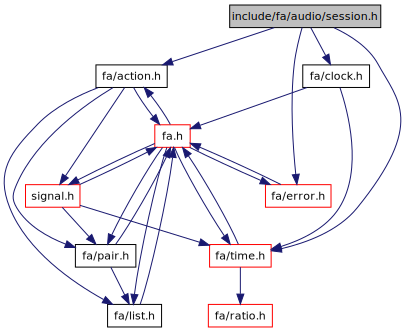
\includegraphics[width=350pt]{audio_2session_8h__incl}
\end{center}
\end{figure}
This graph shows which files directly or indirectly include this file\-:\nopagebreak
\begin{figure}[H]
\begin{center}
\leavevmode
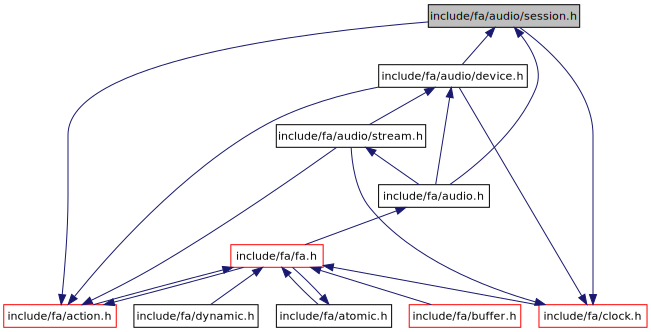
\includegraphics[width=350pt]{audio_2session_8h__dep__incl}
\end{center}
\end{figure}
\subsection*{Typedefs}
\begin{DoxyCompactItemize}
\item 
typedef struct \\*
\-\_\-fa\-\_\-audio\-\_\-session\-\_\-t $\ast$ \hyperlink{group___fa_audio_session_ga62ee22268c23f1b18447141feccc01e0}{fa\-\_\-audio\-\_\-session\-\_\-t}
\begin{DoxyCompactList}\small\item\em An audio session. \end{DoxyCompactList}\item 
typedef \hyperlink{group___fa_audio_session_ga62ee22268c23f1b18447141feccc01e0}{fa\-\_\-audio\-\_\-session\-\_\-t}($\ast$ \hyperlink{group___fa_audio_session_gafd8f3afd0f59b1df855bbc368c2ec419}{fa\-\_\-audio\-\_\-session\-\_\-callback\-\_\-t} )(\hyperlink{group___fa_ga915ddeae99ad7568b273d2b876425197}{fa\-\_\-ptr\-\_\-t}, \hyperlink{group___fa_audio_session_ga62ee22268c23f1b18447141feccc01e0}{fa\-\_\-audio\-\_\-session\-\_\-t})
\begin{DoxyCompactList}\small\item\em A callback to receive audio sessions. \end{DoxyCompactList}\item 
typedef \hyperlink{group___fa_ga43b940a9294fd58a54087ef0b416e479}{fa\-\_\-nullary\-\_\-t} \hyperlink{group___fa_audio_session_gaac3fa018078a475e6c5ed48efcbdb887}{fa\-\_\-audio\-\_\-status\-\_\-callback\-\_\-t}
\begin{DoxyCompactList}\small\item\em A callback to be invoked upon changes to the audio setup. \end{DoxyCompactList}\end{DoxyCompactItemize}
\subsection*{Functions}
\begin{DoxyCompactItemize}
\item 
\hyperlink{group___fa_audio_session_ga62ee22268c23f1b18447141feccc01e0}{fa\-\_\-audio\-\_\-session\-\_\-t} \hyperlink{group___fa_audio_session_ga0022e6e72ee2f2c4c04a6165847a50dd}{fa\-\_\-audio\-\_\-begin\-\_\-session} ()
\begin{DoxyCompactList}\small\item\em Begin a new audio session. \end{DoxyCompactList}\item 
void \hyperlink{group___fa_audio_session_ga2fb042b6c0cbedf65c85a0dbb38c134b}{fa\-\_\-audio\-\_\-end\-\_\-session} (\hyperlink{group___fa_audio_session_ga62ee22268c23f1b18447141feccc01e0}{fa\-\_\-audio\-\_\-session\-\_\-t} session)
\begin{DoxyCompactList}\small\item\em End the given session. \end{DoxyCompactList}\item 
void \hyperlink{group___fa_audio_session_gabbec6678e24f6476ac04f7d759ec7ffb}{fa\-\_\-audio\-\_\-with\-\_\-session} (\hyperlink{group___fa_audio_session_gafd8f3afd0f59b1df855bbc368c2ec419}{fa\-\_\-audio\-\_\-session\-\_\-callback\-\_\-t} session\-Callback, \hyperlink{group___fa_ga915ddeae99ad7568b273d2b876425197}{fa\-\_\-ptr\-\_\-t} ptr, \hyperlink{group___fa_error_ga43d8d45a005130a5052ba3281a8bf33e}{fa\-\_\-error\-\_\-callback\-\_\-t} callback, \hyperlink{group___fa_ga915ddeae99ad7568b273d2b876425197}{fa\-\_\-ptr\-\_\-t} ptr\-\_\-)
\begin{DoxyCompactList}\small\item\em Begin a new session, and retain it for the duration of a call to the given function. \end{DoxyCompactList}\item 
void \hyperlink{group___fa_audio_session_ga82566075d8bfad3afa67fb982dc5d1a9}{fa\-\_\-audio\-\_\-set\-\_\-parameter} (\hyperlink{group___fa_string_gacada63033b77bc6c39fa632ae199349b}{fa\-\_\-string\-\_\-t} \hyperlink{util_8h_a41106000aac73b61e4fc2ef9dd39a603}{string}, \hyperlink{group___fa_ga915ddeae99ad7568b273d2b876425197}{fa\-\_\-ptr\-\_\-t} ptr, \hyperlink{group___fa_audio_session_ga62ee22268c23f1b18447141feccc01e0}{fa\-\_\-audio\-\_\-session\-\_\-t} session)
\begin{DoxyCompactList}\small\item\em Set an audio parameter value. \end{DoxyCompactList}\item 
\hyperlink{group___fa_list_ga35ecb12ab934ded0cce0bcf28e3bc5d2}{fa\-\_\-list\-\_\-t} \hyperlink{group___fa_audio_session_ga4ca512f9ca05840d737cc947e278dd19}{fa\-\_\-audio\-\_\-current\-\_\-sessions} ()
\begin{DoxyCompactList}\small\item\em Get all currently active audio sessions. \end{DoxyCompactList}\item 
\hyperlink{group___fa_ga915ddeae99ad7568b273d2b876425197}{fa\-\_\-ptr\-\_\-t} \hyperlink{group___fa_audio_session_ga8fe894dde7fe548e4c8e20a79609919d}{fa\-\_\-audio\-\_\-end\-\_\-all\-\_\-sessions} ()
\begin{DoxyCompactList}\small\item\em End all currently active audio sessions. \end{DoxyCompactList}\item 
\hyperlink{group___fa_list_ga35ecb12ab934ded0cce0bcf28e3bc5d2}{fa\-\_\-list\-\_\-t} \hyperlink{group___fa_audio_session_ga6ca6844a8e2e55157571335d5cb7a446}{fa\-\_\-audio\-\_\-all} (\hyperlink{group___fa_audio_session_ga62ee22268c23f1b18447141feccc01e0}{fa\-\_\-audio\-\_\-session\-\_\-t} session)
\begin{DoxyCompactList}\small\item\em Get all active audio devices of the given session. \end{DoxyCompactList}\end{DoxyCompactItemize}

\hypertarget{midi_2session_8h}{\section{include/fa/midi/session.h File Reference}
\label{midi_2session_8h}\index{include/fa/midi/session.\-h@{include/fa/midi/session.\-h}}
}

\hypertarget{audio_2stream_8h}{\section{include/fa/audio/stream.h File Reference}
\label{audio_2stream_8h}\index{include/fa/audio/stream.\-h@{include/fa/audio/stream.\-h}}
}
{\ttfamily \#include $<$fa/action.\-h$>$}\\*
{\ttfamily \#include $<$fa/time.\-h$>$}\\*
{\ttfamily \#include $<$fa/clock.\-h$>$}\\*
{\ttfamily \#include $<$fa/list.\-h$>$}\\*
{\ttfamily \#include $<$fa/pair.\-h$>$}\\*
{\ttfamily \#include $<$fa/error.\-h$>$}\\*
{\ttfamily \#include $<$fa/signal.\-h$>$}\\*
{\ttfamily \#include $<$fa/audio/device.\-h$>$}\\*
Include dependency graph for stream.\-h\-:\nopagebreak
\begin{figure}[H]
\begin{center}
\leavevmode
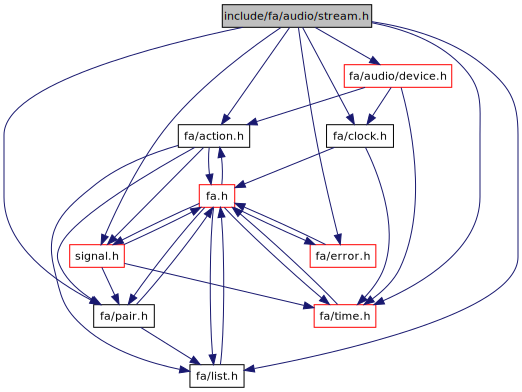
\includegraphics[width=350pt]{audio_2stream_8h__incl}
\end{center}
\end{figure}
This graph shows which files directly or indirectly include this file\-:\nopagebreak
\begin{figure}[H]
\begin{center}
\leavevmode
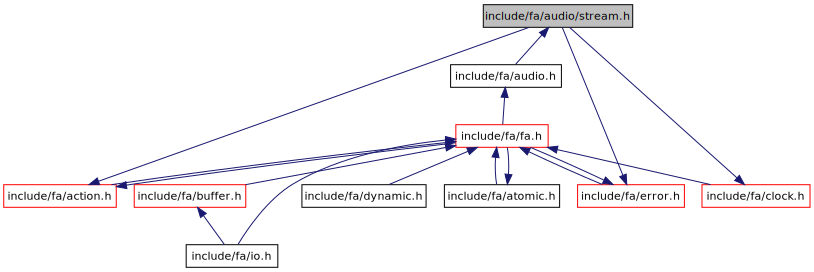
\includegraphics[width=350pt]{audio_2stream_8h__dep__incl}
\end{center}
\end{figure}
\subsection*{Typedefs}
\begin{DoxyCompactItemize}
\item 
typedef struct \-\_\-fa\-\_\-audio\-\_\-stream\-\_\-t $\ast$ \hyperlink{group___fa_audio_stream_ga78fbee3026130ce00d8e00a4e73a84c3}{fa\-\_\-audio\-\_\-stream\-\_\-t}
\begin{DoxyCompactList}\small\item\em An audio stream. \end{DoxyCompactList}\item 
typedef \hyperlink{group___fa_gaaafae8ab9ebae9019133108e56d2d4d1}{fa\-\_\-unary\-\_\-t} \hyperlink{group___fa_audio_stream_gaee8c48d438acabf22f2dfa3b85a4196c}{fa\-\_\-audio\-\_\-message\-\_\-callback\-\_\-t}
\begin{DoxyCompactList}\small\item\em A callback to be invoked whenever a message is received. \end{DoxyCompactList}\item 
typedef \hyperlink{group___fa_audio_stream_ga78fbee3026130ce00d8e00a4e73a84c3}{fa\-\_\-audio\-\_\-stream\-\_\-t}($\ast$ \hyperlink{group___fa_audio_stream_gab6aa7a7bed246893a5cb6d20d2e53199}{fa\-\_\-audio\-\_\-stream\-\_\-callback\-\_\-t} )(\hyperlink{group___fa_ga915ddeae99ad7568b273d2b876425197}{fa\-\_\-ptr\-\_\-t}, \hyperlink{group___fa_audio_stream_ga78fbee3026130ce00d8e00a4e73a84c3}{fa\-\_\-audio\-\_\-stream\-\_\-t})
\begin{DoxyCompactList}\small\item\em A callback to receive audio streams. \end{DoxyCompactList}\end{DoxyCompactItemize}
\subsection*{Functions}
\begin{DoxyCompactItemize}
\item 
\hyperlink{group___fa_audio_stream_ga78fbee3026130ce00d8e00a4e73a84c3}{fa\-\_\-audio\-\_\-stream\-\_\-t} \hyperlink{group___fa_audio_stream_ga912f03969d6207dd40a2746e62888adb}{fa\-\_\-audio\-\_\-open\-\_\-stream} (\hyperlink{group___fa_audio_device_ga03de89ee66c6465f8cedd3a0286598f4}{fa\-\_\-audio\-\_\-device\-\_\-t} device, \hyperlink{group___fa_audio_device_ga03de89ee66c6465f8cedd3a0286598f4}{fa\-\_\-audio\-\_\-device\-\_\-t} device\-\_\-, \hyperlink{group___fa_audio_device_gae190189bb20427f20453f2e4d48ecc7b}{fa\-\_\-audio\-\_\-proc\-\_\-t} proc, \hyperlink{group___fa_ga915ddeae99ad7568b273d2b876425197}{fa\-\_\-ptr\-\_\-t} ptr)
\begin{DoxyCompactList}\small\item\em Open a stream on the given devices. \end{DoxyCompactList}\item 
void \hyperlink{group___fa_audio_stream_ga79df3c5ef2dd7844fe00aa24f0a53d2e}{fa\-\_\-audio\-\_\-close\-\_\-stream} (\hyperlink{group___fa_audio_stream_ga78fbee3026130ce00d8e00a4e73a84c3}{fa\-\_\-audio\-\_\-stream\-\_\-t} stream)
\begin{DoxyCompactList}\small\item\em Close the given stream. \end{DoxyCompactList}\item 
void \hyperlink{group___fa_audio_stream_gaa385a92b31401915477027e03a39094e}{fa\-\_\-audio\-\_\-with\-\_\-stream} (\hyperlink{group___fa_audio_device_ga03de89ee66c6465f8cedd3a0286598f4}{fa\-\_\-audio\-\_\-device\-\_\-t} device, \hyperlink{group___fa_audio_device_ga03de89ee66c6465f8cedd3a0286598f4}{fa\-\_\-audio\-\_\-device\-\_\-t} device\-\_\-, \hyperlink{group___fa_audio_device_gae190189bb20427f20453f2e4d48ecc7b}{fa\-\_\-audio\-\_\-proc\-\_\-t} proc, \hyperlink{group___fa_ga915ddeae99ad7568b273d2b876425197}{fa\-\_\-ptr\-\_\-t} ptr, \hyperlink{group___fa_audio_stream_gab6aa7a7bed246893a5cb6d20d2e53199}{fa\-\_\-audio\-\_\-stream\-\_\-callback\-\_\-t} stream\-Callback, \hyperlink{group___fa_ga915ddeae99ad7568b273d2b876425197}{fa\-\_\-ptr\-\_\-t} ptr\-\_\-, \hyperlink{group___fa_error_ga43d8d45a005130a5052ba3281a8bf33e}{fa\-\_\-error\-\_\-callback\-\_\-t} callback, \hyperlink{group___fa_ga915ddeae99ad7568b273d2b876425197}{fa\-\_\-ptr\-\_\-t} ptr\-\_\-\-\_\-)
\begin{DoxyCompactList}\small\item\em Run a stream on the given devices. \end{DoxyCompactList}\item 
\hyperlink{group___fa_list_ga35ecb12ab934ded0cce0bcf28e3bc5d2}{fa\-\_\-list\-\_\-t} \hyperlink{group___fa_audio_stream_gac4e606b56619fb93da2ad08a29124b99}{fa\-\_\-audio\-\_\-devices} (\hyperlink{group___fa_audio_stream_ga78fbee3026130ce00d8e00a4e73a84c3}{fa\-\_\-audio\-\_\-stream\-\_\-t} stream)
\begin{DoxyCompactList}\small\item\em Return the devices associated with the given stream. \end{DoxyCompactList}\item 
\hyperlink{group___fa_clock_ga20b3a0f49788fbedba140b1d315d2313}{fa\-\_\-clock\-\_\-t} \hyperlink{group___fa_audio_stream_gafeddb7f975954c8d586af0d3a7043f93}{fa\-\_\-audio\-\_\-get\-\_\-clock} (\hyperlink{group___fa_audio_stream_ga78fbee3026130ce00d8e00a4e73a84c3}{fa\-\_\-audio\-\_\-stream\-\_\-t} stream)
\begin{DoxyCompactList}\small\item\em Return the clock associated with a given stream. \end{DoxyCompactList}\item 
\hyperlink{group___fa_clock_ga20b3a0f49788fbedba140b1d315d2313}{fa\-\_\-clock\-\_\-t} \hyperlink{group___fa_audio_stream_ga4d3c49d217cb3e8cebea323261997840}{fa\-\_\-audio\-\_\-stream\-\_\-clock} (\hyperlink{group___fa_audio_stream_ga78fbee3026130ce00d8e00a4e73a84c3}{fa\-\_\-audio\-\_\-stream\-\_\-t} stream)
\begin{DoxyCompactList}\small\item\em Return the clock associated with a given stream. \end{DoxyCompactList}\item 
void \hyperlink{group___fa_audio_stream_gace71cd35b253e3891f1742667fd1be68}{fa\-\_\-audio\-\_\-add\-\_\-message\-\_\-callback} (\hyperlink{group___fa_audio_stream_gaee8c48d438acabf22f2dfa3b85a4196c}{fa\-\_\-audio\-\_\-message\-\_\-callback\-\_\-t} callback, \hyperlink{group___fa_ga915ddeae99ad7568b273d2b876425197}{fa\-\_\-ptr\-\_\-t} callback\-Data, \hyperlink{group___fa_audio_stream_ga78fbee3026130ce00d8e00a4e73a84c3}{fa\-\_\-audio\-\_\-stream\-\_\-t} session)
\begin{DoxyCompactList}\small\item\em Register a callback to be invoked when a message is received. \end{DoxyCompactList}\item 
void \hyperlink{group___fa_audio_stream_gad98527accbfa2dcd59124577eac422bc}{fa\-\_\-audio\-\_\-schedule} (\hyperlink{group___fa_time_ga227cc693f20b4873fed11028bcade184}{fa\-\_\-time\-\_\-t} time, \hyperlink{group___fa_action_gadb08ae063168671e5fedc6c23f20ae4b}{fa\-\_\-action\-\_\-t} action, \hyperlink{group___fa_audio_stream_ga78fbee3026130ce00d8e00a4e73a84c3}{fa\-\_\-audio\-\_\-stream\-\_\-t} stream)
\begin{DoxyCompactList}\small\item\em Schedule an action on the stream. \end{DoxyCompactList}\item 
void \hyperlink{group___fa_audio_stream_ga4283ce1b2c9605c1b5086e2439ae6ce4}{fa\-\_\-audio\-\_\-schedule\-\_\-relative} (\hyperlink{group___fa_time_ga227cc693f20b4873fed11028bcade184}{fa\-\_\-time\-\_\-t} time, \hyperlink{group___fa_action_gadb08ae063168671e5fedc6c23f20ae4b}{fa\-\_\-action\-\_\-t} action, \hyperlink{group___fa_audio_stream_ga78fbee3026130ce00d8e00a4e73a84c3}{fa\-\_\-audio\-\_\-stream\-\_\-t} stream)
\begin{DoxyCompactList}\small\item\em Schedule an action on the stream. \end{DoxyCompactList}\end{DoxyCompactItemize}

\hypertarget{midi_2stream_8h}{\section{include/fa/midi/stream.h File Reference}
\label{midi_2stream_8h}\index{include/fa/midi/stream.\-h@{include/fa/midi/stream.\-h}}
}

\hypertarget{buffer_8h}{\section{include/fa/buffer.h File Reference}
\label{buffer_8h}\index{include/fa/buffer.\-h@{include/fa/buffer.\-h}}
}
{\ttfamily \#include $<$fa.\-h$>$}\\*
{\ttfamily \#include $<$fa/std.\-h$>$}\\*
{\ttfamily \#include $<$fa/pair.\-h$>$}\\*
{\ttfamily \#include $<$fa/string.\-h$>$}\\*
{\ttfamily \#include $<$fa/map.\-h$>$}\\*
Include dependency graph for buffer.\-h\-:\nopagebreak
\begin{figure}[H]
\begin{center}
\leavevmode
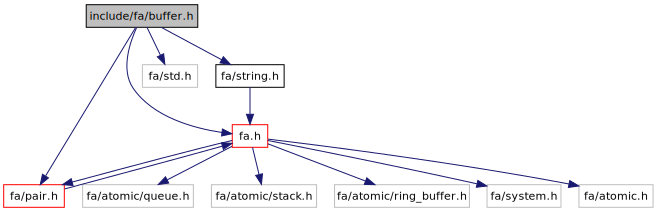
\includegraphics[width=350pt]{buffer_8h__incl}
\end{center}
\end{figure}
This graph shows which files directly or indirectly include this file\-:\nopagebreak
\begin{figure}[H]
\begin{center}
\leavevmode
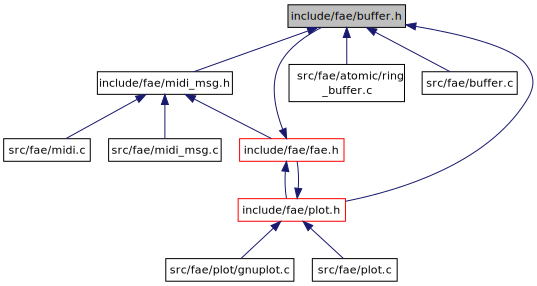
\includegraphics[width=350pt]{buffer_8h__dep__incl}
\end{center}
\end{figure}
\subsection*{Typedefs}
\begin{DoxyCompactItemize}
\item 
typedef struct \-\_\-fa\-\_\-buffer\-\_\-t $\ast$ \hyperlink{group___fa_buffer_ga0ed7a1d783ab322e2e8be02432d0839e}{fa\-\_\-buffer\-\_\-t}
\begin{DoxyCompactList}\small\item\em The buffer. \end{DoxyCompactList}\end{DoxyCompactItemize}
\subsection*{Functions}
\begin{DoxyCompactItemize}
\item 
\hyperlink{group___fa_buffer_ga0ed7a1d783ab322e2e8be02432d0839e}{fa\-\_\-buffer\-\_\-t} \hyperlink{group___fa_buffer_ga67c4124d193bca81a6e21ec04d9ff832}{fa\-\_\-buffer\-\_\-create} (size\-\_\-t size\-\_\-)
\begin{DoxyCompactList}\small\item\em Create a new buffer and initialize it to zero-\/bytes. \end{DoxyCompactList}\item 
\hyperlink{group___fa_buffer_ga0ed7a1d783ab322e2e8be02432d0839e}{fa\-\_\-buffer\-\_\-t} \hyperlink{group___fa_buffer_gabc24b8a0d76fcd92c1f9071c34a55704}{fa\-\_\-buffer\-\_\-wrap} (\hyperlink{group___fa_ga915ddeae99ad7568b273d2b876425197}{fa\-\_\-ptr\-\_\-t} ptr, size\-\_\-t size\-\_\-, \hyperlink{group___fa_gaaafae8ab9ebae9019133108e56d2d4d1}{fa\-\_\-unary\-\_\-t} unary, \hyperlink{group___fa_ga915ddeae99ad7568b273d2b876425197}{fa\-\_\-ptr\-\_\-t} ptr\-\_\-)
\begin{DoxyCompactList}\small\item\em Create a buffer wrapping the given memory region. \end{DoxyCompactList}\item 
\hyperlink{group___fa_buffer_ga0ed7a1d783ab322e2e8be02432d0839e}{fa\-\_\-buffer\-\_\-t} \hyperlink{group___fa_buffer_ga11c1b1ce03700c52a38ff4f87cc0eeec}{fa\-\_\-buffer\-\_\-copy} (\hyperlink{group___fa_buffer_ga0ed7a1d783ab322e2e8be02432d0839e}{fa\-\_\-buffer\-\_\-t} \hyperlink{util_8h_ad0c623e8b04565926f5b48888327724a}{buffer})
\begin{DoxyCompactList}\small\item\em Copy the given buffer. \end{DoxyCompactList}\item 
\hyperlink{group___fa_buffer_ga0ed7a1d783ab322e2e8be02432d0839e}{fa\-\_\-buffer\-\_\-t} \hyperlink{group___fa_buffer_ga2e0379c378fad447bc00890b4c55d0f9}{fa\-\_\-buffer\-\_\-resize} (size\-\_\-t size\-\_\-, \hyperlink{group___fa_buffer_ga0ed7a1d783ab322e2e8be02432d0839e}{fa\-\_\-buffer\-\_\-t} \hyperlink{util_8h_ad0c623e8b04565926f5b48888327724a}{buffer})
\begin{DoxyCompactList}\small\item\em Return a new buffer of the given size containing the contents of the given buffer padded with zero bytes at the end. \end{DoxyCompactList}\item 
\hyperlink{group___fa_buffer_ga0ed7a1d783ab322e2e8be02432d0839e}{fa\-\_\-buffer\-\_\-t} \hyperlink{group___fa_buffer_gab569f84162545bb4426a2d426ace8950}{fa\-\_\-buffer\-\_\-dresize} (size\-\_\-t size\-\_\-, \hyperlink{group___fa_buffer_ga0ed7a1d783ab322e2e8be02432d0839e}{fa\-\_\-buffer\-\_\-t} \hyperlink{util_8h_ad0c623e8b04565926f5b48888327724a}{buffer})
\begin{DoxyCompactList}\small\item\em Return a new buffer of the given size containing the contents of the given buffer padded with zero bytes at the end. \end{DoxyCompactList}\item 
void \hyperlink{group___fa_buffer_ga51af4022b7ccfc33f8ee0862c8bbad5e}{fa\-\_\-buffer\-\_\-destroy} (\hyperlink{group___fa_buffer_ga0ed7a1d783ab322e2e8be02432d0839e}{fa\-\_\-buffer\-\_\-t} \hyperlink{util_8h_ad0c623e8b04565926f5b48888327724a}{buffer})
\begin{DoxyCompactList}\small\item\em Destroy the given buffer. \end{DoxyCompactList}\item 
size\-\_\-t \hyperlink{group___fa_buffer_ga412e71a916e24b101f9b8a967b4d53f8}{fa\-\_\-buffer\-\_\-size} (\hyperlink{group___fa_buffer_ga0ed7a1d783ab322e2e8be02432d0839e}{fa\-\_\-buffer\-\_\-t} \hyperlink{util_8h_ad0c623e8b04565926f5b48888327724a}{buffer})
\begin{DoxyCompactList}\small\item\em Return the size of the buffer. \end{DoxyCompactList}\item 
\hyperlink{group___fa_ga915ddeae99ad7568b273d2b876425197}{fa\-\_\-ptr\-\_\-t} \hyperlink{group___fa_buffer_gaf21b86142b1246b676f9bfbeb54011aa}{fa\-\_\-buffer\-\_\-get\-\_\-meta} (\hyperlink{group___fa_buffer_ga0ed7a1d783ab322e2e8be02432d0839e}{fa\-\_\-buffer\-\_\-t} \hyperlink{util_8h_ad0c623e8b04565926f5b48888327724a}{buffer}, \hyperlink{group___fa_string_gacada63033b77bc6c39fa632ae199349b}{fa\-\_\-string\-\_\-t} \hyperlink{util_8h_a41106000aac73b61e4fc2ef9dd39a603}{string})
\begin{DoxyCompactList}\small\item\em Get the value of some meta-\/data attribute of the given buffer. \end{DoxyCompactList}\item 
void \hyperlink{group___fa_buffer_gac2efb810e723accb6f7e8f0ae5651a80}{fa\-\_\-buffer\-\_\-set\-\_\-meta} (\hyperlink{group___fa_buffer_ga0ed7a1d783ab322e2e8be02432d0839e}{fa\-\_\-buffer\-\_\-t} \hyperlink{util_8h_ad0c623e8b04565926f5b48888327724a}{buffer}, \hyperlink{group___fa_string_gacada63033b77bc6c39fa632ae199349b}{fa\-\_\-string\-\_\-t} \hyperlink{util_8h_a41106000aac73b61e4fc2ef9dd39a603}{string}, \hyperlink{group___fa_ga915ddeae99ad7568b273d2b876425197}{fa\-\_\-ptr\-\_\-t} ptr)
\begin{DoxyCompactList}\small\item\em Set the value of some meta-\/data attribute of the given buffer. \end{DoxyCompactList}\item 
\hyperlink{group___fa_map_gadcbb0c425af31be6aeb265159b2a7db0}{fa\-\_\-map\-\_\-t} \hyperlink{group___fa_buffer_ga8cae6305af4695da927f707f00e530bd}{fa\-\_\-buffer\-\_\-meta} (\hyperlink{group___fa_buffer_ga0ed7a1d783ab322e2e8be02432d0839e}{fa\-\_\-buffer\-\_\-t} \hyperlink{util_8h_ad0c623e8b04565926f5b48888327724a}{buffer})
\begin{DoxyCompactList}\small\item\em Get all meta-\/data as a map from strings to values. \end{DoxyCompactList}\item 
uint8\-\_\-t \hyperlink{group___fa_buffer_ga6a4d986aa6ce7023563bc9f3e3dd416f}{fa\-\_\-buffer\-\_\-get} (\hyperlink{group___fa_buffer_ga0ed7a1d783ab322e2e8be02432d0839e}{fa\-\_\-buffer\-\_\-t} \hyperlink{util_8h_ad0c623e8b04565926f5b48888327724a}{buffer}, size\-\_\-t size\-\_\-)
\begin{DoxyCompactList}\small\item\em Get a value from the buffer. \end{DoxyCompactList}\item 
void \hyperlink{group___fa_buffer_ga2ba7ad9f2ad61d4d908eedb862c99474}{fa\-\_\-buffer\-\_\-set} (\hyperlink{group___fa_buffer_ga0ed7a1d783ab322e2e8be02432d0839e}{fa\-\_\-buffer\-\_\-t} \hyperlink{util_8h_ad0c623e8b04565926f5b48888327724a}{buffer}, size\-\_\-t size\-\_\-, uint8\-\_\-t u\-Int8\-\_\-)
\begin{DoxyCompactList}\small\item\em Update a value in the buffer. \end{DoxyCompactList}\item 
\hyperlink{group___fa_buffer_ga0ed7a1d783ab322e2e8be02432d0839e}{fa\-\_\-buffer\-\_\-t} \hyperlink{group___fa_buffer_ga3aa381eabd42a82492cec36b0f2dced4}{fa\-\_\-buffer\-\_\-take} (size\-\_\-t size\-\_\-, \hyperlink{group___fa_buffer_ga0ed7a1d783ab322e2e8be02432d0839e}{fa\-\_\-buffer\-\_\-t} \hyperlink{util_8h_ad0c623e8b04565926f5b48888327724a}{buffer})
\begin{DoxyCompactList}\small\item\em Copy the first n bytes. \end{DoxyCompactList}\item 
\hyperlink{group___fa_buffer_ga0ed7a1d783ab322e2e8be02432d0839e}{fa\-\_\-buffer\-\_\-t} \hyperlink{group___fa_buffer_ga0d057fff991ddc68b23635c3bef09111}{fa\-\_\-buffer\-\_\-drop} (size\-\_\-t size\-\_\-, \hyperlink{group___fa_buffer_ga0ed7a1d783ab322e2e8be02432d0839e}{fa\-\_\-buffer\-\_\-t} \hyperlink{util_8h_ad0c623e8b04565926f5b48888327724a}{buffer})
\begin{DoxyCompactList}\small\item\em Copy from the given number of bytes. \end{DoxyCompactList}\item 
\hyperlink{group___fa_pair_gac2b2e58c230bac4f8a63ef6c05072680}{fa\-\_\-pair\-\_\-t} \hyperlink{group___fa_buffer_gac7d4196d3cdf0c3221d27f8c982e00f2}{fa\-\_\-buffer\-\_\-take\-\_\-drop} (size\-\_\-t size\-\_\-, \hyperlink{group___fa_buffer_ga0ed7a1d783ab322e2e8be02432d0839e}{fa\-\_\-buffer\-\_\-t} \hyperlink{util_8h_ad0c623e8b04565926f5b48888327724a}{buffer})
\begin{DoxyCompactList}\small\item\em Efficient combination of take and drop. \end{DoxyCompactList}\item 
\hyperlink{group___fa_list_ga35ecb12ab934ded0cce0bcf28e3bc5d2}{fa\-\_\-list\-\_\-t} \hyperlink{group___fa_buffer_ga270797e37d8d7b94321ee7636407a5d3}{fa\-\_\-buffer\-\_\-split} (\hyperlink{group___fa_buffer_ga0ed7a1d783ab322e2e8be02432d0839e}{fa\-\_\-buffer\-\_\-t} \hyperlink{util_8h_ad0c623e8b04565926f5b48888327724a}{buffer}, size\-\_\-t size\-\_\-)
\begin{DoxyCompactList}\small\item\em Split into a list of buffers containing at most n bytes. \end{DoxyCompactList}\item 
int16\-\_\-t \hyperlink{group___fa_buffer_ga8179fe2b2edda4927721fd5a45d2e18c}{fa\-\_\-buffer\-\_\-get\-\_\-int16} (\hyperlink{group___fa_buffer_ga0ed7a1d783ab322e2e8be02432d0839e}{fa\-\_\-buffer\-\_\-t} \hyperlink{util_8h_ad0c623e8b04565926f5b48888327724a}{buffer}, size\-\_\-t size\-\_\-)
\begin{DoxyCompactList}\small\item\em Get a value from the buffer. \end{DoxyCompactList}\item 
int32\-\_\-t \hyperlink{group___fa_buffer_ga51609720018ae6391083205b260db9a7}{fa\-\_\-buffer\-\_\-get\-\_\-int32} (\hyperlink{group___fa_buffer_ga0ed7a1d783ab322e2e8be02432d0839e}{fa\-\_\-buffer\-\_\-t} \hyperlink{util_8h_ad0c623e8b04565926f5b48888327724a}{buffer}, size\-\_\-t size\-\_\-)
\begin{DoxyCompactList}\small\item\em Get a value from the buffer. \end{DoxyCompactList}\item 
int64\-\_\-t \hyperlink{group___fa_buffer_gad596c5b40ca8ce644eff53140aa3d8c9}{fa\-\_\-buffer\-\_\-get\-\_\-int64} (\hyperlink{group___fa_buffer_ga0ed7a1d783ab322e2e8be02432d0839e}{fa\-\_\-buffer\-\_\-t} \hyperlink{util_8h_ad0c623e8b04565926f5b48888327724a}{buffer}, size\-\_\-t size\-\_\-)
\begin{DoxyCompactList}\small\item\em Get a value from the buffer. \end{DoxyCompactList}\item 
float \hyperlink{group___fa_buffer_gaf317e894970857eee2b1e315e6b341ee}{fa\-\_\-buffer\-\_\-get\-\_\-float} (\hyperlink{group___fa_buffer_ga0ed7a1d783ab322e2e8be02432d0839e}{fa\-\_\-buffer\-\_\-t} \hyperlink{util_8h_ad0c623e8b04565926f5b48888327724a}{buffer}, size\-\_\-t size\-\_\-)
\begin{DoxyCompactList}\small\item\em Get a value from the buffer. \end{DoxyCompactList}\item 
double \hyperlink{group___fa_buffer_gae6416e46d9dc795feb4dad5a45b381b5}{fa\-\_\-buffer\-\_\-get\-\_\-double} (\hyperlink{group___fa_buffer_ga0ed7a1d783ab322e2e8be02432d0839e}{fa\-\_\-buffer\-\_\-t} \hyperlink{util_8h_ad0c623e8b04565926f5b48888327724a}{buffer}, size\-\_\-t size\-\_\-)
\begin{DoxyCompactList}\small\item\em Get a value from the buffer. \end{DoxyCompactList}\item 
void \hyperlink{group___fa_buffer_gaddf42d41a14338e04f83f854dc264f2d}{fa\-\_\-buffer\-\_\-set\-\_\-int16} (\hyperlink{group___fa_buffer_ga0ed7a1d783ab322e2e8be02432d0839e}{fa\-\_\-buffer\-\_\-t} \hyperlink{util_8h_ad0c623e8b04565926f5b48888327724a}{buffer}, size\-\_\-t size\-\_\-, int16\-\_\-t int16\-\_\-)
\begin{DoxyCompactList}\small\item\em Update a value in the buffer. \end{DoxyCompactList}\item 
void \hyperlink{group___fa_buffer_gaa29344ea6962a2e728ba96e3837b7608}{fa\-\_\-buffer\-\_\-set\-\_\-int32} (\hyperlink{group___fa_buffer_ga0ed7a1d783ab322e2e8be02432d0839e}{fa\-\_\-buffer\-\_\-t} \hyperlink{util_8h_ad0c623e8b04565926f5b48888327724a}{buffer}, size\-\_\-t size\-\_\-, int32\-\_\-t int32\-\_\-)
\begin{DoxyCompactList}\small\item\em Update a value in the buffer. \end{DoxyCompactList}\item 
void \hyperlink{group___fa_buffer_gaa9703d8e4b82d5640c8fdfeb8ad5068f}{fa\-\_\-buffer\-\_\-set\-\_\-int64} (\hyperlink{group___fa_buffer_ga0ed7a1d783ab322e2e8be02432d0839e}{fa\-\_\-buffer\-\_\-t} \hyperlink{util_8h_ad0c623e8b04565926f5b48888327724a}{buffer}, size\-\_\-t size\-\_\-, int64\-\_\-t int64\-\_\-)
\begin{DoxyCompactList}\small\item\em Update a value in the buffer. \end{DoxyCompactList}\item 
void \hyperlink{group___fa_buffer_gad2df4ce0cc602042aafd794636f5abe3}{fa\-\_\-buffer\-\_\-set\-\_\-float} (\hyperlink{group___fa_buffer_ga0ed7a1d783ab322e2e8be02432d0839e}{fa\-\_\-buffer\-\_\-t} \hyperlink{util_8h_ad0c623e8b04565926f5b48888327724a}{buffer}, size\-\_\-t size\-\_\-, float float\-\_\-)
\begin{DoxyCompactList}\small\item\em Update a value in the buffer. \end{DoxyCompactList}\item 
void \hyperlink{group___fa_buffer_gaa0ebad825c6e97124c1aabeaf17e3631}{fa\-\_\-buffer\-\_\-set\-\_\-double} (\hyperlink{group___fa_buffer_ga0ed7a1d783ab322e2e8be02432d0839e}{fa\-\_\-buffer\-\_\-t} \hyperlink{util_8h_ad0c623e8b04565926f5b48888327724a}{buffer}, size\-\_\-t size\-\_\-, double double\-\_\-)
\begin{DoxyCompactList}\small\item\em Update a value in the buffer. \end{DoxyCompactList}\item 
\hyperlink{group___fa_buffer_ga0ed7a1d783ab322e2e8be02432d0839e}{fa\-\_\-buffer\-\_\-t} \hyperlink{group___fa_buffer_gaf2ee73288b08b98a94fa831731e5b261}{fa\-\_\-buffer\-\_\-read\-\_\-raw} (\hyperlink{group___fa_string_gacada63033b77bc6c39fa632ae199349b}{fa\-\_\-string\-\_\-t} \hyperlink{util_8h_a41106000aac73b61e4fc2ef9dd39a603}{string})
\begin{DoxyCompactList}\small\item\em Reads a buffer from a file. \end{DoxyCompactList}\item 
void \hyperlink{group___fa_buffer_gaf423ff710d861b91fe833e60c860ec7a}{fa\-\_\-buffer\-\_\-write\-\_\-raw} (\hyperlink{group___fa_string_gacada63033b77bc6c39fa632ae199349b}{fa\-\_\-string\-\_\-t} \hyperlink{util_8h_a41106000aac73b61e4fc2ef9dd39a603}{string}, \hyperlink{group___fa_buffer_ga0ed7a1d783ab322e2e8be02432d0839e}{fa\-\_\-buffer\-\_\-t} \hyperlink{util_8h_ad0c623e8b04565926f5b48888327724a}{buffer})
\begin{DoxyCompactList}\small\item\em Write a buffer to a file. \end{DoxyCompactList}\item 
\hyperlink{group___fa_pair_gac2b2e58c230bac4f8a63ef6c05072680}{fa\-\_\-pair\-\_\-t} \hyperlink{group___fa_buffer_gadf31c6e905d0207931790f3468862940}{fa\-\_\-buffer\-\_\-read\-\_\-audio} (\hyperlink{group___fa_string_gacada63033b77bc6c39fa632ae199349b}{fa\-\_\-string\-\_\-t} \hyperlink{util_8h_a41106000aac73b61e4fc2ef9dd39a603}{string})
\begin{DoxyCompactList}\small\item\em Read an audio file. \end{DoxyCompactList}\item 
\hyperlink{group___fa_ga915ddeae99ad7568b273d2b876425197}{fa\-\_\-ptr\-\_\-t} \hyperlink{group___fa_buffer_ga51462ff7c74f09e7ea59d80895544558}{fa\-\_\-buffer\-\_\-write\-\_\-audio} (\hyperlink{group___fa_string_gacada63033b77bc6c39fa632ae199349b}{fa\-\_\-string\-\_\-t} \hyperlink{util_8h_a41106000aac73b61e4fc2ef9dd39a603}{string}, int int\-\_\-, \hyperlink{group___fa_buffer_ga0ed7a1d783ab322e2e8be02432d0839e}{fa\-\_\-buffer\-\_\-t} \hyperlink{util_8h_ad0c623e8b04565926f5b48888327724a}{buffer})
\begin{DoxyCompactList}\small\item\em Write an audio file. \end{DoxyCompactList}\item 
void $\ast$ \hyperlink{group___fa_buffer_gae70cd25a1633cea1ad12bc6080f3cd29}{fa\-\_\-buffer\-\_\-unsafe\-\_\-address} (\hyperlink{group___fa_buffer_ga0ed7a1d783ab322e2e8be02432d0839e}{fa\-\_\-buffer\-\_\-t} \hyperlink{util_8h_ad0c623e8b04565926f5b48888327724a}{buffer})
\begin{DoxyCompactList}\small\item\em Return the address of the buffer. \end{DoxyCompactList}\end{DoxyCompactItemize}

\hypertarget{clock_8h}{\section{include/fa/clock.h File Reference}
\label{clock_8h}\index{include/fa/clock.\-h@{include/fa/clock.\-h}}
}
{\ttfamily \#include $<$fa.\-h$>$}\\*
{\ttfamily \#include $<$fa/time.\-h$>$}\\*
Include dependency graph for clock.\-h\-:\nopagebreak
\begin{figure}[H]
\begin{center}
\leavevmode
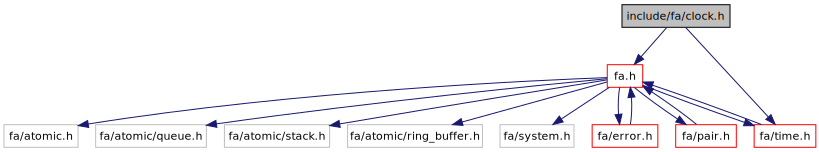
\includegraphics[width=350pt]{clock_8h__incl}
\end{center}
\end{figure}
This graph shows which files directly or indirectly include this file\-:\nopagebreak
\begin{figure}[H]
\begin{center}
\leavevmode
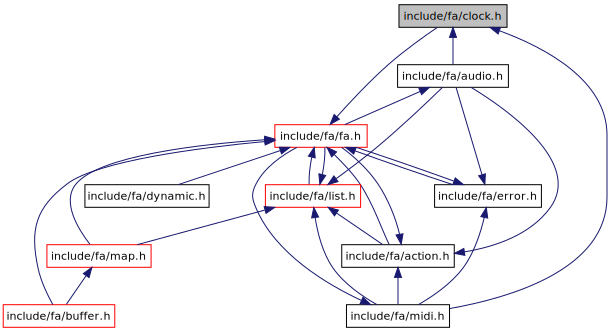
\includegraphics[width=350pt]{clock_8h__dep__incl}
\end{center}
\end{figure}
\subsection*{Data Structures}
\begin{DoxyCompactItemize}
\item 
struct \hyperlink{structfa__clock__interface__t}{fa\-\_\-clock\-\_\-interface\-\_\-t}
\end{DoxyCompactItemize}
\subsection*{Typedefs}
\begin{DoxyCompactItemize}
\item 
typedef struct \-\_\-fa\-\_\-clock\-\_\-t $\ast$ \hyperlink{group___fa_clock_ga20b3a0f49788fbedba140b1d315d2313}{fa\-\_\-clock\-\_\-t}
\begin{DoxyCompactList}\small\item\em A value of an unknown type implementing \hyperlink{structfa__clock__interface__t}{fa\-\_\-clock\-\_\-interface\-\_\-t}. \end{DoxyCompactList}\end{DoxyCompactItemize}
\subsection*{Functions}
\begin{DoxyCompactItemize}
\item 
\hyperlink{group___fa_time_ga227cc693f20b4873fed11028bcade184}{fa\-\_\-time\-\_\-t} \hyperlink{group___fa_clock_ga18d53d2bcd2ff1618760b9960e40d56d}{fa\-\_\-clock\-\_\-time} (\hyperlink{group___fa_clock_ga20b3a0f49788fbedba140b1d315d2313}{fa\-\_\-clock\-\_\-t} clock)
\begin{DoxyCompactList}\small\item\em Returns the current time according to the given clock. \end{DoxyCompactList}\item 
\hyperlink{group___fa_time_gadebdebeab6c5ba7cd8002d0773635e61}{fa\-\_\-time\-\_\-milliseconds\-\_\-t} \hyperlink{group___fa_clock_gad09133a7293cd31a05d99b8915546a4a}{fa\-\_\-clock\-\_\-milliseconds} (\hyperlink{group___fa_clock_ga20b3a0f49788fbedba140b1d315d2313}{fa\-\_\-clock\-\_\-t} clock)
\begin{DoxyCompactList}\small\item\em Returns the current time in milliseconds according to the given clock. \end{DoxyCompactList}\item 
\hyperlink{group___fa_clock_ga20b3a0f49788fbedba140b1d315d2313}{fa\-\_\-clock\-\_\-t} \hyperlink{group___fa_clock_ga867297b309d28fdf6e47bf259eb6f914}{fa\-\_\-clock\-\_\-standard} ()
\begin{DoxyCompactList}\small\item\em Returns the standard clock. \end{DoxyCompactList}\end{DoxyCompactItemize}

\hypertarget{dynamic_8h}{\section{include/fa/dynamic.h File Reference}
\label{dynamic_8h}\index{include/fa/dynamic.\-h@{include/fa/dynamic.\-h}}
}
{\ttfamily \#include $<$fa.\-h$>$}\\*
{\ttfamily \#include $<$fa/string.\-h$>$}\\*
Include dependency graph for dynamic.\-h\-:\nopagebreak
\begin{figure}[H]
\begin{center}
\leavevmode
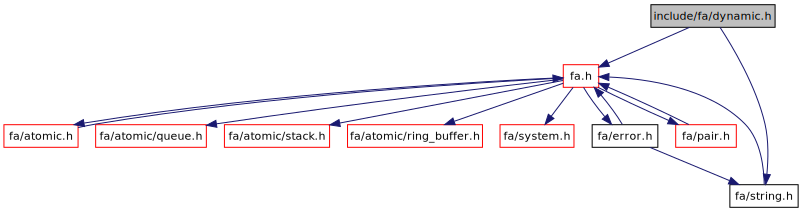
\includegraphics[width=350pt]{dynamic_8h__incl}
\end{center}
\end{figure}
\subsection*{Data Structures}
\begin{DoxyCompactItemize}
\item 
struct \hyperlink{structfa__dynamic__t}{fa\-\_\-dynamic\-\_\-t}
\begin{DoxyCompactList}\small\item\em Dynamic typing interface. \end{DoxyCompactList}\end{DoxyCompactItemize}
\subsection*{Enumerations}
\begin{DoxyCompactItemize}
\item 
enum \hyperlink{group___fa_dynamic_ga38427e999172dad2684f07793859f416}{fa\-\_\-dynamic\-\_\-type\-\_\-repr\-\_\-t} \{ \\*
\hyperlink{group___fa_dynamic_gga38427e999172dad2684f07793859f416a650f8740967e93fd6bd505be9e66da25}{bool\-\_\-type\-\_\-repr}, 
\hyperlink{group___fa_dynamic_gga38427e999172dad2684f07793859f416aa143afc69e19795fe8ad3ec810a3350f}{i8\-\_\-type\-\_\-repr}, 
\hyperlink{group___fa_dynamic_gga38427e999172dad2684f07793859f416a749a639c18497875eb6ca2c659979483}{i16\-\_\-type\-\_\-repr}, 
\hyperlink{group___fa_dynamic_gga38427e999172dad2684f07793859f416a986d45d849f556447a754059537f7619}{i32\-\_\-type\-\_\-repr}, 
\\*
\hyperlink{group___fa_dynamic_gga38427e999172dad2684f07793859f416a3cd2e66183bfd3acb4893d951c84c439}{i64\-\_\-type\-\_\-repr}, 
\hyperlink{group___fa_dynamic_gga38427e999172dad2684f07793859f416a9569f7b88a9725a95dc6d2450c2d09f3}{f32\-\_\-type\-\_\-repr}, 
\hyperlink{group___fa_dynamic_gga38427e999172dad2684f07793859f416a36db315441705cc136fb6b1c4116e824}{f64\-\_\-type\-\_\-repr}, 
\hyperlink{group___fa_dynamic_gga38427e999172dad2684f07793859f416a3a2e655a4d66c724b28570d35a16acdb}{pair\-\_\-type\-\_\-repr}, 
\\*
\hyperlink{group___fa_dynamic_gga38427e999172dad2684f07793859f416ad4ff103381c3edaa488857cfb6b49ab7}{list\-\_\-type\-\_\-repr}, 
\hyperlink{group___fa_dynamic_gga38427e999172dad2684f07793859f416abbf0c6c59d19b853ceb62ef8f252f8e4}{set\-\_\-type\-\_\-repr}, 
\hyperlink{group___fa_dynamic_gga38427e999172dad2684f07793859f416a86521286e4ad90b519c91a2c62ab67ad}{map\-\_\-type\-\_\-repr}, 
\hyperlink{group___fa_dynamic_gga38427e999172dad2684f07793859f416a2d776384cbeaba2666b0e05f3b8b7a56}{string\-\_\-type\-\_\-repr}, 
\\*
\hyperlink{group___fa_dynamic_gga38427e999172dad2684f07793859f416ad4a0998e1b4d7b4cbbe31ee7ff033101}{ratio\-\_\-type\-\_\-repr}
 \}
\end{DoxyCompactItemize}
\subsection*{Functions}
\begin{DoxyCompactItemize}
\item 
bool \hyperlink{group___fa_dynamic_ga98007c81126e3255272875dd53ea0e10}{fa\-\_\-dynamic\-\_\-check} (\hyperlink{group___fa_ga915ddeae99ad7568b273d2b876425197}{fa\-\_\-ptr\-\_\-t} ptr)
\begin{DoxyCompactList}\small\item\em Whether the given value supports dynamic typing. \end{DoxyCompactList}\item 
\hyperlink{group___fa_dynamic_ga38427e999172dad2684f07793859f416}{fa\-\_\-dynamic\-\_\-type\-\_\-repr\-\_\-t} \hyperlink{group___fa_dynamic_ga75682ebb43d63500c11d24909c84c6ba}{fa\-\_\-dynamic\-\_\-get\-\_\-type} (\hyperlink{group___fa_ga915ddeae99ad7568b273d2b876425197}{fa\-\_\-ptr\-\_\-t} ptr)
\begin{DoxyCompactList}\small\item\em Returns a value representating the the type of the given value, which must implement \hyperlink{structfa__dynamic__t}{fa\-\_\-dynamic\-\_\-t}. \end{DoxyCompactList}\end{DoxyCompactItemize}

\hypertarget{error_8h}{\section{include/fa/error.h File Reference}
\label{error_8h}\index{include/fa/error.\-h@{include/fa/error.\-h}}
}
{\ttfamily \#include $<$fa.\-h$>$}\\*
{\ttfamily \#include $<$fa/string.\-h$>$}\\*
Include dependency graph for error.\-h\-:\nopagebreak
\begin{figure}[H]
\begin{center}
\leavevmode
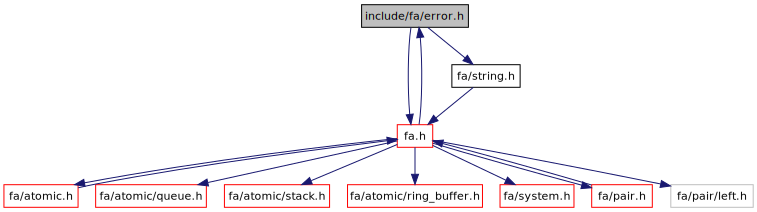
\includegraphics[width=350pt]{error_8h__incl}
\end{center}
\end{figure}
This graph shows which files directly or indirectly include this file\-:\nopagebreak
\begin{figure}[H]
\begin{center}
\leavevmode
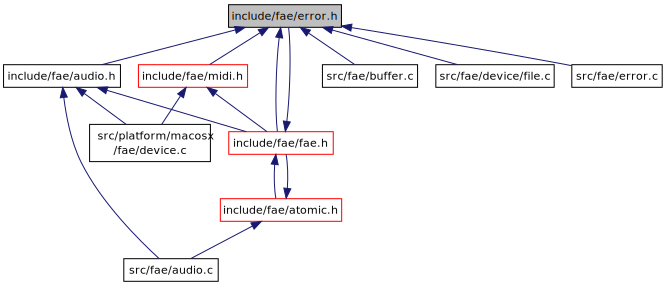
\includegraphics[width=350pt]{error_8h__dep__incl}
\end{center}
\end{figure}
\subsection*{Data Structures}
\begin{DoxyCompactItemize}
\item 
struct \hyperlink{structfa__error__interface__t}{fa\-\_\-error\-\_\-interface\-\_\-t}
\begin{DoxyCompactList}\small\item\em Error interface. \end{DoxyCompactList}\end{DoxyCompactItemize}
\subsection*{Typedefs}
\begin{DoxyCompactItemize}
\item 
typedef struct \-\_\-fa\-\_\-error\-\_\-t $\ast$ \hyperlink{group___fa_error_ga4a4feb4d3686657ac8dbd2be421cbb15}{fa\-\_\-error\-\_\-t}
\begin{DoxyCompactList}\small\item\em A type implementing \hyperlink{structfa__error__interface__t}{fa\-\_\-error\-\_\-interface\-\_\-t}. \end{DoxyCompactList}\item 
typedef void($\ast$ \hyperlink{group___fa_error_ga43d8d45a005130a5052ba3281a8bf33e}{fa\-\_\-error\-\_\-callback\-\_\-t} )(\hyperlink{group___fa_ga915ddeae99ad7568b273d2b876425197}{fa\-\_\-ptr\-\_\-t}, \hyperlink{group___fa_error_ga4a4feb4d3686657ac8dbd2be421cbb15}{fa\-\_\-error\-\_\-t})
\begin{DoxyCompactList}\small\item\em An error handler routine. \end{DoxyCompactList}\end{DoxyCompactItemize}
\subsection*{Enumerations}
\begin{DoxyCompactItemize}
\item 
enum \hyperlink{group___fa_error_ga5cf5c13f1e12ae6b125c0265f59f4d82}{fa\-\_\-error\-\_\-severity\-\_\-t} \{ \hyperlink{group___fa_error_gga5cf5c13f1e12ae6b125c0265f59f4d82aa4abb266e72efba828327b605b2ab0f4}{info}, 
\hyperlink{group___fa_error_gga5cf5c13f1e12ae6b125c0265f59f4d82a8de9aef05fc85e519a0cfce33573f492}{warning}, 
\hyperlink{group___fa_error_gga5cf5c13f1e12ae6b125c0265f59f4d82ad606e435413ea0944dd00d49e901e4ed}{error}, 
\hyperlink{group___fa_error_gga5cf5c13f1e12ae6b125c0265f59f4d82a8e61437747405a9d1a65e5020e375e08}{misc}
 \}
\end{DoxyCompactItemize}
\subsection*{Functions}
\begin{DoxyCompactItemize}
\item 
bool \hyperlink{group___fa_error_gab7550192e471f82582ecb441949c8b62}{fa\-\_\-error\-\_\-check} (\hyperlink{group___fa_ga915ddeae99ad7568b273d2b876425197}{fa\-\_\-ptr\-\_\-t} ptr)
\begin{DoxyCompactList}\small\item\em Return whether the given value is an error or not. \end{DoxyCompactList}\item 
void \hyperlink{group___fa_error_ga466e0539bedb29f68527448ed9ba11bf}{fa\-\_\-error\-\_\-log} (\hyperlink{group___fa_ga915ddeae99ad7568b273d2b876425197}{fa\-\_\-ptr\-\_\-t} ptr, \hyperlink{group___fa_error_ga4a4feb4d3686657ac8dbd2be421cbb15}{fa\-\_\-error\-\_\-t} \hyperlink{group___fa_error_gga5cf5c13f1e12ae6b125c0265f59f4d82ad606e435413ea0944dd00d49e901e4ed}{error})
\begin{DoxyCompactList}\small\item\em Write a log message. \end{DoxyCompactList}\item 
\hyperlink{group___fa_error_ga5cf5c13f1e12ae6b125c0265f59f4d82}{fa\-\_\-error\-\_\-severity\-\_\-t} \hyperlink{group___fa_error_ga260bea83fbb420ad257323648c86cd15}{fa\-\_\-error\-\_\-severity} (\hyperlink{group___fa_error_ga4a4feb4d3686657ac8dbd2be421cbb15}{fa\-\_\-error\-\_\-t} \hyperlink{group___fa_error_gga5cf5c13f1e12ae6b125c0265f59f4d82ad606e435413ea0944dd00d49e901e4ed}{error})
\begin{DoxyCompactList}\small\item\em Return the severity of the given error. \end{DoxyCompactList}\item 
\hyperlink{group___fa_string_gacada63033b77bc6c39fa632ae199349b}{fa\-\_\-string\-\_\-t} \hyperlink{group___fa_error_ga8539a91f951952f94c4270a0f04f6ad1}{fa\-\_\-error\-\_\-message} (\hyperlink{group___fa_error_ga4a4feb4d3686657ac8dbd2be421cbb15}{fa\-\_\-error\-\_\-t} \hyperlink{group___fa_error_gga5cf5c13f1e12ae6b125c0265f59f4d82ad606e435413ea0944dd00d49e901e4ed}{error})
\begin{DoxyCompactList}\small\item\em Return the message of the given error. \end{DoxyCompactList}\item 
\hyperlink{group___fa_string_gacada63033b77bc6c39fa632ae199349b}{fa\-\_\-string\-\_\-t} \hyperlink{group___fa_error_ga1bb041273b8f969a8c2d7bd292141110}{fa\-\_\-error\-\_\-origin} (\hyperlink{group___fa_error_ga4a4feb4d3686657ac8dbd2be421cbb15}{fa\-\_\-error\-\_\-t} \hyperlink{group___fa_error_gga5cf5c13f1e12ae6b125c0265f59f4d82ad606e435413ea0944dd00d49e901e4ed}{error})
\begin{DoxyCompactList}\small\item\em Return the origin of the given error. \end{DoxyCompactList}\item 
\hyperlink{group___fa_string_gacada63033b77bc6c39fa632ae199349b}{fa\-\_\-string\-\_\-t} \hyperlink{group___fa_error_ga0ecd2e70e166904907ed98f102d1d59a}{fa\-\_\-error\-\_\-format} (bool bool\-\_\-, \hyperlink{group___fa_error_ga4a4feb4d3686657ac8dbd2be421cbb15}{fa\-\_\-error\-\_\-t} \hyperlink{group___fa_error_gga5cf5c13f1e12ae6b125c0265f59f4d82ad606e435413ea0944dd00d49e901e4ed}{error})
\begin{DoxyCompactList}\small\item\em Convert the given error to a formated string. \end{DoxyCompactList}\item 
\hyperlink{group___fa_error_ga4a4feb4d3686657ac8dbd2be421cbb15}{fa\-\_\-error\-\_\-t} \hyperlink{group___fa_error_gadd811b06a5cd740039902f77efd4e661}{fa\-\_\-error\-\_\-create\-\_\-simple} (\hyperlink{group___fa_error_ga5cf5c13f1e12ae6b125c0265f59f4d82}{fa\-\_\-error\-\_\-severity\-\_\-t} severity, \hyperlink{group___fa_string_gacada63033b77bc6c39fa632ae199349b}{fa\-\_\-string\-\_\-t} \hyperlink{util_8h_a41106000aac73b61e4fc2ef9dd39a603}{string}, \hyperlink{group___fa_string_gacada63033b77bc6c39fa632ae199349b}{fa\-\_\-string\-\_\-t} string\-\_\-)
\begin{DoxyCompactList}\small\item\em Creates a simple error. \end{DoxyCompactList}\end{DoxyCompactItemize}

\hypertarget{fa_2fa_8h}{\section{include/fa/fa.h File Reference}
\label{fa_2fa_8h}\index{include/fa/fa.\-h@{include/fa/fa.\-h}}
}
{\ttfamily \#include $<$fa/atomic.\-h$>$}\\*
{\ttfamily \#include $<$fa/atomic/queue.\-h$>$}\\*
{\ttfamily \#include $<$fa/atomic/stack.\-h$>$}\\*
{\ttfamily \#include $<$fa/atomic/ring\-\_\-buffer.\-h$>$}\\*
{\ttfamily \#include $<$fa/system.\-h$>$}\\*
{\ttfamily \#include $<$fa/error.\-h$>$}\\*
{\ttfamily \#include $<$fa/pair.\-h$>$}\\*
{\ttfamily \#include $<$fa/pair/left.\-h$>$}\\*
{\ttfamily \#include $<$fa/list.\-h$>$}\\*
{\ttfamily \#include $<$fa/audio.\-h$>$}\\*
{\ttfamily \#include $<$fa/midi.\-h$>$}\\*
{\ttfamily \#include $<$fa/midi/message.\-h$>$}\\*
{\ttfamily \#include $<$fa/thread.\-h$>$}\\*
{\ttfamily \#include $<$fa/time.\-h$>$}\\*
{\ttfamily \#include $<$fa/priority\-\_\-queue.\-h$>$}\\*
{\ttfamily \#include $<$fa/action.\-h$>$}\\*
{\ttfamily \#include $<$fa/signal.\-h$>$}\\*
This graph shows which files directly or indirectly include this file\-:\nopagebreak
\begin{figure}[H]
\begin{center}
\leavevmode
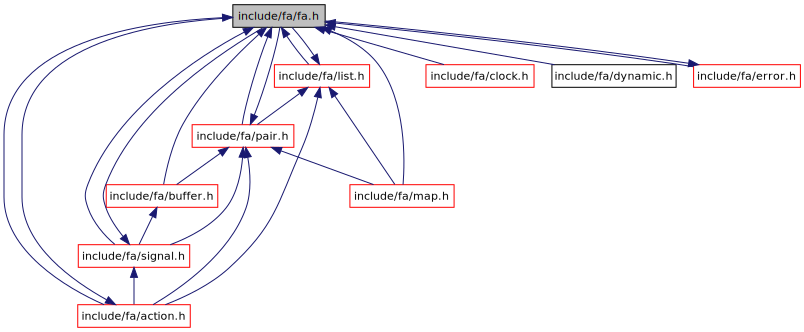
\includegraphics[width=350pt]{fa_2fa_8h__dep__incl}
\end{center}
\end{figure}
\subsection*{Typedefs}
\begin{DoxyCompactItemize}
\item 
typedef void($\ast$ \hyperlink{group___fa_utility_ga1f914d0c16f566e96a08db3a3446aab7}{fa\-\_\-log\-\_\-func\-\_\-t} )(\hyperlink{group___fa_ga915ddeae99ad7568b273d2b876425197}{fa\-\_\-ptr\-\_\-t}, \hyperlink{group___fa_time_ga7dd7e28574eec80380aac22be7087d2e}{fa\-\_\-time\-\_\-system\-\_\-t}, \hyperlink{group___fa_error_ga4a4feb4d3686657ac8dbd2be421cbb15}{fa\-\_\-error\-\_\-t})
\end{DoxyCompactItemize}
\subsection*{Functions}
\begin{DoxyCompactItemize}
\item 
\hyperlink{group___fa_list_ga35ecb12ab934ded0cce0bcf28e3bc5d2}{fa\-\_\-list\-\_\-t} \hyperlink{group___fa_utility_ga10bbb957eedee5b2a3c8e91a169f9991}{fa\-\_\-version} ()
\begin{DoxyCompactList}\small\item\em Returns the version of Fa as a list on the form {\ttfamily (\char`\"{}alpha\char`\"{}, 1, 0, 5, \char`\"{}\char`\"{})}. \end{DoxyCompactList}\item 
\hyperlink{group___fa_string_gacada63033b77bc6c39fa632ae199349b}{fa\-\_\-string\-\_\-t} \hyperlink{group___fa_utility_ga0f32aba533df7023c5d0948d6506b94e}{fa\-\_\-version\-\_\-string} ()
\begin{DoxyCompactList}\small\item\em Returns the version of Fa as a string on the form \char`\"{}alpha1.\-0.\-5\char`\"{}. \end{DoxyCompactList}\item 
void \hyperlink{group___fa_utility_ga061c945c3f013c84561593911b661a44}{fa\-\_\-initialize} ()
\begin{DoxyCompactList}\small\item\em Performs global initialization. \end{DoxyCompactList}\item 
void \hyperlink{group___fa_utility_ga66c7af3a85045329f71966dfe40a5acf}{fa\-\_\-terminate} ()
\begin{DoxyCompactList}\small\item\em Performs global cleanup. \end{DoxyCompactList}\item 
void \hyperlink{group___fa_utility_ga09490b15451aa64808537eb688aa4604}{fa\-\_\-set\-\_\-log\-\_\-file} (\hyperlink{group___fa_string_gacada63033b77bc6c39fa632ae199349b}{fa\-\_\-string\-\_\-t} \hyperlink{util_8h_a41106000aac73b61e4fc2ef9dd39a603}{string})
\begin{DoxyCompactList}\small\item\em Instruct Fa to write log messages to the specific file. \end{DoxyCompactList}\item 
void \hyperlink{group___fa_utility_gaadd396f69e7ae709c4e224d893ff90a6}{fa\-\_\-set\-\_\-log\-\_\-std} ()
\begin{DoxyCompactList}\small\item\em Instruct Fa to write log messages to the standard output. \end{DoxyCompactList}\item 
void \hyperlink{group___fa_utility_ga97a486eb85c974972eebfd7d69eaa8c3}{fa\-\_\-set\-\_\-log} (\hyperlink{group___fa_utility_ga1f914d0c16f566e96a08db3a3446aab7}{fa\-\_\-log\-\_\-func\-\_\-t} log\-Func, \hyperlink{group___fa_ga915ddeae99ad7568b273d2b876425197}{fa\-\_\-ptr\-\_\-t} ptr)
\begin{DoxyCompactList}\small\item\em Instruct Fa to pass log messages to the given handler. \end{DoxyCompactList}\item 
void \hyperlink{group___fa_utility_ga9567a792b3679742c7ab6535c368be60}{fa\-\_\-log} (\hyperlink{group___fa_ga915ddeae99ad7568b273d2b876425197}{fa\-\_\-ptr\-\_\-t} ptr, \hyperlink{group___fa_error_ga4a4feb4d3686657ac8dbd2be421cbb15}{fa\-\_\-error\-\_\-t} \hyperlink{group___fa_error_gga5cf5c13f1e12ae6b125c0265f59f4d82ad606e435413ea0944dd00d49e901e4ed}{error})
\begin{DoxyCompactList}\small\item\em Write a log message. \end{DoxyCompactList}\item 
void \hyperlink{group___fa_utility_ga7d0eec2d02accbcf65148ea41e680b1e}{fa\-\_\-log\-\_\-info} (\hyperlink{group___fa_string_gacada63033b77bc6c39fa632ae199349b}{fa\-\_\-string\-\_\-t} \hyperlink{util_8h_a41106000aac73b61e4fc2ef9dd39a603}{string})
\begin{DoxyCompactList}\small\item\em Write an informative message to the log. \end{DoxyCompactList}\item 
void \hyperlink{group___fa_utility_gaadbae9a73993245706ca501b11b531ec}{fa\-\_\-log\-\_\-warning} (\hyperlink{group___fa_string_gacada63033b77bc6c39fa632ae199349b}{fa\-\_\-string\-\_\-t} \hyperlink{util_8h_a41106000aac73b61e4fc2ef9dd39a603}{string})
\begin{DoxyCompactList}\small\item\em Write a warning to the log. \end{DoxyCompactList}\item 
void \hyperlink{group___fa_utility_gaf6025219b330102e95a473aa2450bd7f}{fa\-\_\-log\-\_\-error} (\hyperlink{group___fa_string_gacada63033b77bc6c39fa632ae199349b}{fa\-\_\-string\-\_\-t} \hyperlink{util_8h_a41106000aac73b61e4fc2ef9dd39a603}{string})
\begin{DoxyCompactList}\small\item\em Write an error to the log. \end{DoxyCompactList}\item 
void \hyperlink{group___fa_utility_ga0c1973f20d36a9af40e69f4fb6237126}{fa\-\_\-log\-\_\-info\-\_\-from} (\hyperlink{group___fa_string_gacada63033b77bc6c39fa632ae199349b}{fa\-\_\-string\-\_\-t} \hyperlink{util_8h_a41106000aac73b61e4fc2ef9dd39a603}{string}, \hyperlink{group___fa_string_gacada63033b77bc6c39fa632ae199349b}{fa\-\_\-string\-\_\-t} string\-\_\-)
\begin{DoxyCompactList}\small\item\em Write an informative message to the log. \end{DoxyCompactList}\item 
void \hyperlink{group___fa_utility_gaa1508f7cf8794e99da97612ac76e694b}{fa\-\_\-log\-\_\-warning\-\_\-from} (\hyperlink{group___fa_string_gacada63033b77bc6c39fa632ae199349b}{fa\-\_\-string\-\_\-t} \hyperlink{util_8h_a41106000aac73b61e4fc2ef9dd39a603}{string}, \hyperlink{group___fa_string_gacada63033b77bc6c39fa632ae199349b}{fa\-\_\-string\-\_\-t} string\-\_\-)
\begin{DoxyCompactList}\small\item\em Write a warning to the log. \end{DoxyCompactList}\item 
void \hyperlink{group___fa_utility_gad90cd8e846dfbeabe3572e2e4f842204}{fa\-\_\-log\-\_\-error\-\_\-from} (\hyperlink{group___fa_string_gacada63033b77bc6c39fa632ae199349b}{fa\-\_\-string\-\_\-t} \hyperlink{util_8h_a41106000aac73b61e4fc2ef9dd39a603}{string}, \hyperlink{group___fa_string_gacada63033b77bc6c39fa632ae199349b}{fa\-\_\-string\-\_\-t} string\-\_\-)
\begin{DoxyCompactList}\small\item\em Write an error to the log. \end{DoxyCompactList}\end{DoxyCompactItemize}

\hypertarget{fa_8h}{\section{include/fa.h File Reference}
\label{fa_8h}\index{include/fa.\-h@{include/fa.\-h}}
}
{\ttfamily \#include $<$fa/std.\-h$>$}\\*
{\ttfamily \#include $<$fa/alloc.\-h$>$}\\*
{\ttfamily \#include $<$fa/interfaces.\-h$>$}\\*
Include dependency graph for fa.\-h\-:\nopagebreak
\begin{figure}[H]
\begin{center}
\leavevmode
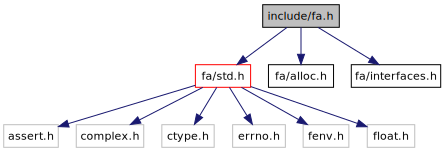
\includegraphics[width=350pt]{fa_8h__incl}
\end{center}
\end{figure}
This graph shows which files directly or indirectly include this file\-:\nopagebreak
\begin{figure}[H]
\begin{center}
\leavevmode
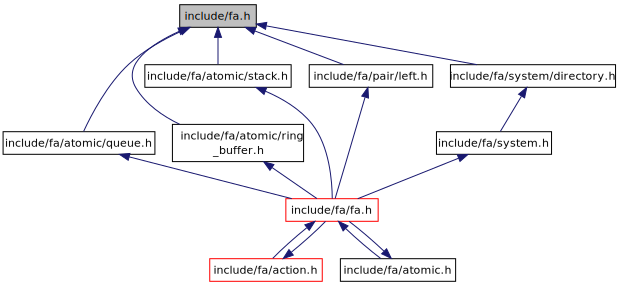
\includegraphics[width=350pt]{fa_8h__dep__incl}
\end{center}
\end{figure}
\subsection*{Data Structures}
\begin{DoxyCompactItemize}
\item 
struct \hyperlink{structfa__equal__t}{fa\-\_\-equal\-\_\-t}
\begin{DoxyCompactList}\small\item\em Equality comparison interface. \end{DoxyCompactList}\item 
struct \hyperlink{structfa__order__t}{fa\-\_\-order\-\_\-t}
\begin{DoxyCompactList}\small\item\em Less-\/than comparison interface. \end{DoxyCompactList}\item 
struct \hyperlink{structfa__number__t}{fa\-\_\-number\-\_\-t}
\begin{DoxyCompactList}\small\item\em Arithmetic operations interface. \end{DoxyCompactList}\item 
struct \hyperlink{structfa__copy__t}{fa\-\_\-copy\-\_\-t}
\begin{DoxyCompactList}\small\item\em Generic copying interface. \end{DoxyCompactList}\item 
struct \hyperlink{structfa__destroy__t}{fa\-\_\-destroy\-\_\-t}
\begin{DoxyCompactList}\small\item\em Generic destruction interface. \end{DoxyCompactList}\end{DoxyCompactItemize}
\subsection*{Typedefs}
\begin{DoxyCompactItemize}
\item 
typedef void $\ast$ \hyperlink{group___fa_ga915ddeae99ad7568b273d2b876425197}{fa\-\_\-ptr\-\_\-t}
\begin{DoxyCompactList}\small\item\em Pointer type, equivalent to {\ttfamily void$\ast$}. \end{DoxyCompactList}\item 
typedef \hyperlink{group___fa_ga915ddeae99ad7568b273d2b876425197}{fa\-\_\-ptr\-\_\-t}($\ast$ \hyperlink{group___fa_ga43b940a9294fd58a54087ef0b416e479}{fa\-\_\-nullary\-\_\-t} )(\hyperlink{group___fa_ga915ddeae99ad7568b273d2b876425197}{fa\-\_\-ptr\-\_\-t})
\begin{DoxyCompactList}\small\item\em A nullary function, defined as {\ttfamily fa\-\_\-ptr\-\_\-t($\ast$fa\-\_\-nullary\-\_\-t )(fa\-\_\-ptr\-\_\-t)}. \end{DoxyCompactList}\item 
typedef \hyperlink{group___fa_ga915ddeae99ad7568b273d2b876425197}{fa\-\_\-ptr\-\_\-t}($\ast$ \hyperlink{group___fa_gaaafae8ab9ebae9019133108e56d2d4d1}{fa\-\_\-unary\-\_\-t} )(\hyperlink{group___fa_ga915ddeae99ad7568b273d2b876425197}{fa\-\_\-ptr\-\_\-t}, \hyperlink{group___fa_ga915ddeae99ad7568b273d2b876425197}{fa\-\_\-ptr\-\_\-t})
\begin{DoxyCompactList}\small\item\em A unary function. \end{DoxyCompactList}\item 
typedef \hyperlink{group___fa_ga915ddeae99ad7568b273d2b876425197}{fa\-\_\-ptr\-\_\-t}($\ast$ \hyperlink{group___fa_gab70ba406935a18c1d645d12e7abf2e63}{fa\-\_\-binary\-\_\-t} )(\hyperlink{group___fa_ga915ddeae99ad7568b273d2b876425197}{fa\-\_\-ptr\-\_\-t}, \hyperlink{group___fa_ga915ddeae99ad7568b273d2b876425197}{fa\-\_\-ptr\-\_\-t}, \hyperlink{group___fa_ga915ddeae99ad7568b273d2b876425197}{fa\-\_\-ptr\-\_\-t})
\begin{DoxyCompactList}\small\item\em A binary function. \end{DoxyCompactList}\item 
typedef \hyperlink{group___fa_ga915ddeae99ad7568b273d2b876425197}{fa\-\_\-ptr\-\_\-t}($\ast$ \hyperlink{group___fa_gadbab7e8e405b3d2436de1e1126cc4817}{fa\-\_\-ternary\-\_\-t} )(\hyperlink{group___fa_ga915ddeae99ad7568b273d2b876425197}{fa\-\_\-ptr\-\_\-t}, \hyperlink{group___fa_ga915ddeae99ad7568b273d2b876425197}{fa\-\_\-ptr\-\_\-t}, \hyperlink{group___fa_ga915ddeae99ad7568b273d2b876425197}{fa\-\_\-ptr\-\_\-t}, \hyperlink{group___fa_ga915ddeae99ad7568b273d2b876425197}{fa\-\_\-ptr\-\_\-t})
\begin{DoxyCompactList}\small\item\em A ternary function. \end{DoxyCompactList}\item 
typedef bool($\ast$ \hyperlink{group___fa_gae6b6ae9fb073db0ba0bd323d511c6a98}{fa\-\_\-pred\-\_\-t} )(\hyperlink{group___fa_ga915ddeae99ad7568b273d2b876425197}{fa\-\_\-ptr\-\_\-t}, \hyperlink{group___fa_ga915ddeae99ad7568b273d2b876425197}{fa\-\_\-ptr\-\_\-t})
\begin{DoxyCompactList}\small\item\em A predicate, or boolean function. \end{DoxyCompactList}\item 
typedef char \hyperlink{group___fa_ga98bfdb5d0438f95f3438cddeab1818e8}{fa\-\_\-char8\-\_\-t}
\begin{DoxyCompactList}\small\item\em An 8-\/bit character. \end{DoxyCompactList}\item 
typedef uint16\-\_\-t \hyperlink{group___fa_ga33e83372a0abc1895fdad5fb4d15eae3}{fa\-\_\-char16\-\_\-t}
\begin{DoxyCompactList}\small\item\em A 16-\/bit character. \end{DoxyCompactList}\item 
typedef uint32\-\_\-t \hyperlink{group___fa_gaca70e02afbba75b08b2b6531b821f67b}{fa\-\_\-char32\-\_\-t}
\begin{DoxyCompactList}\small\item\em A 32-\/bit character. \end{DoxyCompactList}\item 
typedef int64\-\_\-t \hyperlink{group___fa_gaeb5011c69dfea4d2c41c05a2c95899d0}{fa\-\_\-id\-\_\-t}
\begin{DoxyCompactList}\small\item\em Unique identifier. \end{DoxyCompactList}\item 
typedef \hyperlink{group___fa_ga915ddeae99ad7568b273d2b876425197}{fa\-\_\-ptr\-\_\-t}($\ast$ \hyperlink{group___fa_gac13cc6d4ef02b8763045164333cfd763}{fa\-\_\-impl\-\_\-t} )(\hyperlink{group___fa_gaeb5011c69dfea4d2c41c05a2c95899d0}{fa\-\_\-id\-\_\-t})
\begin{DoxyCompactList}\small\item\em Callback to lookup an interface implementation. \end{DoxyCompactList}\end{DoxyCompactItemize}
\subsection*{Functions}
\begin{DoxyCompactItemize}
\item 
bool \hyperlink{group___fa_gaea204b4c094f2e6fb13a91e22f3f80de}{fa\-\_\-is\-\_\-bool} (\hyperlink{group___fa_ga915ddeae99ad7568b273d2b876425197}{fa\-\_\-ptr\-\_\-t} ptr)
\item 
bool \hyperlink{group___fa_gad0959793c33e61bf126ae45431cce74e}{fa\-\_\-is\-\_\-int8} (\hyperlink{group___fa_ga915ddeae99ad7568b273d2b876425197}{fa\-\_\-ptr\-\_\-t} ptr)
\item 
bool \hyperlink{group___fa_gaa63a843cb966ae896513c9fa2eafc82c}{fa\-\_\-is\-\_\-int16} (\hyperlink{group___fa_ga915ddeae99ad7568b273d2b876425197}{fa\-\_\-ptr\-\_\-t} ptr)
\item 
bool \hyperlink{group___fa_gaae5fd4fcfa0d1d306bb7be3a5bf3b238}{fa\-\_\-is\-\_\-int32} (\hyperlink{group___fa_ga915ddeae99ad7568b273d2b876425197}{fa\-\_\-ptr\-\_\-t} ptr)
\item 
bool \hyperlink{group___fa_ga2cb6a7ad52d1cbee60fa2eaa57fde75e}{fa\-\_\-is\-\_\-int64} (\hyperlink{group___fa_ga915ddeae99ad7568b273d2b876425197}{fa\-\_\-ptr\-\_\-t} ptr)
\item 
bool \hyperlink{group___fa_gaf2acf9a74b67d56c155fec11e55d6129}{fa\-\_\-is\-\_\-float} (\hyperlink{group___fa_ga915ddeae99ad7568b273d2b876425197}{fa\-\_\-ptr\-\_\-t} ptr)
\item 
bool \hyperlink{group___fa_ga1faadaefa3dc646cfe78bb01b22b783e}{fa\-\_\-is\-\_\-double} (\hyperlink{group___fa_ga915ddeae99ad7568b273d2b876425197}{fa\-\_\-ptr\-\_\-t} ptr)
\item 
bool \hyperlink{group___fa_gaa7ee523c4d3f4aea6d3e061d4e52c634}{fa\-\_\-is\-\_\-ref} (\hyperlink{group___fa_ga915ddeae99ad7568b273d2b876425197}{fa\-\_\-ptr\-\_\-t} ptr)
\item 
bool \hyperlink{group___fa_ga55ece575ff8ef52ba6a9ba563ca02a1d}{fa\-\_\-to\-\_\-bool} (\hyperlink{group___fa_ga915ddeae99ad7568b273d2b876425197}{fa\-\_\-ptr\-\_\-t} ptr)
\item 
int8\-\_\-t \hyperlink{group___fa_ga74132ccc642fd868e3dc263f7ad7f6bd}{fa\-\_\-to\-\_\-int8} (\hyperlink{group___fa_ga915ddeae99ad7568b273d2b876425197}{fa\-\_\-ptr\-\_\-t} ptr)
\item 
int16\-\_\-t \hyperlink{group___fa_ga7b88b5b578f58271ba3553d1d46b5576}{fa\-\_\-to\-\_\-int16} (\hyperlink{group___fa_ga915ddeae99ad7568b273d2b876425197}{fa\-\_\-ptr\-\_\-t} ptr)
\item 
int32\-\_\-t \hyperlink{group___fa_gada59a9ba6ae8d62407cc10513c4fc910}{fa\-\_\-to\-\_\-int32} (\hyperlink{group___fa_ga915ddeae99ad7568b273d2b876425197}{fa\-\_\-ptr\-\_\-t} ptr)
\item 
int64\-\_\-t \hyperlink{group___fa_gab4de02370911531a08df105af43946e6}{fa\-\_\-to\-\_\-int64} (\hyperlink{group___fa_ga915ddeae99ad7568b273d2b876425197}{fa\-\_\-ptr\-\_\-t} ptr)
\item 
float \hyperlink{group___fa_ga85cdcb16f8a421d6e3f5fc30588aec3d}{fa\-\_\-to\-\_\-float} (\hyperlink{group___fa_ga915ddeae99ad7568b273d2b876425197}{fa\-\_\-ptr\-\_\-t} ptr)
\item 
double \hyperlink{group___fa_gaf49386f8ba2dbabf3efb756fd7a5fe4c}{fa\-\_\-to\-\_\-double} (\hyperlink{group___fa_ga915ddeae99ad7568b273d2b876425197}{fa\-\_\-ptr\-\_\-t} ptr)
\item 
bool \hyperlink{group___fa_gad1076baa2a1645a19badde8c6ca1e7cf}{fa\-\_\-peek\-\_\-bool} (\hyperlink{group___fa_ga915ddeae99ad7568b273d2b876425197}{fa\-\_\-ptr\-\_\-t} ptr)
\item 
int8\-\_\-t \hyperlink{group___fa_ga526128ab022aab513cd7e8497ae4b6f2}{fa\-\_\-peek\-\_\-int8} (\hyperlink{group___fa_ga915ddeae99ad7568b273d2b876425197}{fa\-\_\-ptr\-\_\-t} ptr)
\item 
int16\-\_\-t \hyperlink{group___fa_ga3adefcb0ba19742209ab8961e77bb248}{fa\-\_\-peek\-\_\-int16} (\hyperlink{group___fa_ga915ddeae99ad7568b273d2b876425197}{fa\-\_\-ptr\-\_\-t} ptr)
\item 
int32\-\_\-t \hyperlink{group___fa_gac8a8358c3e4a1612421e5bf09886e43b}{fa\-\_\-peek\-\_\-int32} (\hyperlink{group___fa_ga915ddeae99ad7568b273d2b876425197}{fa\-\_\-ptr\-\_\-t} ptr)
\item 
int64\-\_\-t \hyperlink{group___fa_ga0206c6d3b07d79924d0f28a93df55474}{fa\-\_\-peek\-\_\-int64} (\hyperlink{group___fa_ga915ddeae99ad7568b273d2b876425197}{fa\-\_\-ptr\-\_\-t} ptr)
\item 
float \hyperlink{group___fa_ga77afde306510c73fb992575d7f2fb91b}{fa\-\_\-peek\-\_\-float} (\hyperlink{group___fa_ga915ddeae99ad7568b273d2b876425197}{fa\-\_\-ptr\-\_\-t} ptr)
\item 
double \hyperlink{group___fa_ga052c5abd5260669679286b36009aaf98}{fa\-\_\-peek\-\_\-double} (\hyperlink{group___fa_ga915ddeae99ad7568b273d2b876425197}{fa\-\_\-ptr\-\_\-t} ptr)
\item 
\hyperlink{group___fa_ga915ddeae99ad7568b273d2b876425197}{fa\-\_\-ptr\-\_\-t} \hyperlink{group___fa_ga03b9cabaaf785a88940eba17bd7ae621}{fa\-\_\-from\-\_\-bool} (bool bool\-\_\-)
\item 
\hyperlink{group___fa_ga915ddeae99ad7568b273d2b876425197}{fa\-\_\-ptr\-\_\-t} \hyperlink{group___fa_gae59bb48493214037997a78b65814ba02}{fa\-\_\-from\-\_\-int8} (int8\-\_\-t int8\-\_\-)
\item 
\hyperlink{group___fa_ga915ddeae99ad7568b273d2b876425197}{fa\-\_\-ptr\-\_\-t} \hyperlink{group___fa_ga2ab9996cc0d378c9c6b3b302011e09a4}{fa\-\_\-from\-\_\-int16} (int16\-\_\-t int16\-\_\-)
\item 
\hyperlink{group___fa_ga915ddeae99ad7568b273d2b876425197}{fa\-\_\-ptr\-\_\-t} \hyperlink{group___fa_gae872f63b8860e24d21166fbabb0d6bc0}{fa\-\_\-from\-\_\-int32} (int32\-\_\-t int32\-\_\-)
\item 
\hyperlink{group___fa_ga915ddeae99ad7568b273d2b876425197}{fa\-\_\-ptr\-\_\-t} \hyperlink{group___fa_gadb00915203c212a107f8fab09328cb39}{fa\-\_\-from\-\_\-int64} (int64\-\_\-t int64\-\_\-)
\item 
\hyperlink{group___fa_ga915ddeae99ad7568b273d2b876425197}{fa\-\_\-ptr\-\_\-t} \hyperlink{group___fa_gae3c3ae262ec23b01ba4664899d89bbc4}{fa\-\_\-from\-\_\-float} (float float\-\_\-)
\item 
\hyperlink{group___fa_ga915ddeae99ad7568b273d2b876425197}{fa\-\_\-ptr\-\_\-t} \hyperlink{group___fa_ga550b80dd4d78000cdd38bd7c3458fd08}{fa\-\_\-from\-\_\-double} (double double\-\_\-)
\item 
\hyperlink{group___fa_ga915ddeae99ad7568b273d2b876425197}{fa\-\_\-ptr\-\_\-t} \hyperlink{group___fa_ga1cc4276643f3d366681ac7ff71fa8b06}{fa\-\_\-interface} (\hyperlink{group___fa_gaeb5011c69dfea4d2c41c05a2c95899d0}{fa\-\_\-id\-\_\-t} id, \hyperlink{group___fa_ga915ddeae99ad7568b273d2b876425197}{fa\-\_\-ptr\-\_\-t} ptr)
\begin{DoxyCompactList}\small\item\em Returns an implenentation of the given interface on the given value. \end{DoxyCompactList}\item 
bool \hyperlink{group___fa_gaded838536607ac403241cde9fd5a4d02}{fa\-\_\-equal} (\hyperlink{group___fa_ga915ddeae99ad7568b273d2b876425197}{fa\-\_\-ptr\-\_\-t} ptr, \hyperlink{group___fa_ga915ddeae99ad7568b273d2b876425197}{fa\-\_\-ptr\-\_\-t} ptr\-\_\-)
\begin{DoxyCompactList}\small\item\em Return whether the given values are equal. \end{DoxyCompactList}\item 
bool \hyperlink{group___fa_ga18edc1c7d73e70df4d925bbc7f125b7f}{fa\-\_\-not\-\_\-equal} (\hyperlink{group___fa_ga915ddeae99ad7568b273d2b876425197}{fa\-\_\-ptr\-\_\-t} ptr, \hyperlink{group___fa_ga915ddeae99ad7568b273d2b876425197}{fa\-\_\-ptr\-\_\-t} ptr\-\_\-)
\begin{DoxyCompactList}\small\item\em Return whether the given values are unequal. \end{DoxyCompactList}\item 
bool \hyperlink{group___fa_ga4747e94dca95afaf031d6b00c36cc8fc}{fa\-\_\-less\-\_\-than} (\hyperlink{group___fa_ga915ddeae99ad7568b273d2b876425197}{fa\-\_\-ptr\-\_\-t} ptr, \hyperlink{group___fa_ga915ddeae99ad7568b273d2b876425197}{fa\-\_\-ptr\-\_\-t} ptr\-\_\-)
\item 
bool \hyperlink{group___fa_ga64d9591f70db8eb11f530b056ac90285}{fa\-\_\-greater\-\_\-than} (\hyperlink{group___fa_ga915ddeae99ad7568b273d2b876425197}{fa\-\_\-ptr\-\_\-t} ptr, \hyperlink{group___fa_ga915ddeae99ad7568b273d2b876425197}{fa\-\_\-ptr\-\_\-t} ptr\-\_\-)
\item 
bool \hyperlink{group___fa_gaf266c6271f28a83627c8ab153ba6fa23}{fa\-\_\-less\-\_\-than\-\_\-equal} (\hyperlink{group___fa_ga915ddeae99ad7568b273d2b876425197}{fa\-\_\-ptr\-\_\-t} ptr, \hyperlink{group___fa_ga915ddeae99ad7568b273d2b876425197}{fa\-\_\-ptr\-\_\-t} ptr\-\_\-)
\item 
bool \hyperlink{group___fa_ga8923b87d5ee72f9976ab4e47aa615a1b}{fa\-\_\-greater\-\_\-than\-\_\-equal} (\hyperlink{group___fa_ga915ddeae99ad7568b273d2b876425197}{fa\-\_\-ptr\-\_\-t} ptr, \hyperlink{group___fa_ga915ddeae99ad7568b273d2b876425197}{fa\-\_\-ptr\-\_\-t} ptr\-\_\-)
\item 
\hyperlink{group___fa_ga915ddeae99ad7568b273d2b876425197}{fa\-\_\-ptr\-\_\-t} \hyperlink{group___fa_ga81600d57c9bde20b7e9be906b1b37447}{fa\-\_\-min} (\hyperlink{group___fa_ga915ddeae99ad7568b273d2b876425197}{fa\-\_\-ptr\-\_\-t} ptr, \hyperlink{group___fa_ga915ddeae99ad7568b273d2b876425197}{fa\-\_\-ptr\-\_\-t} ptr\-\_\-)
\item 
\hyperlink{group___fa_ga915ddeae99ad7568b273d2b876425197}{fa\-\_\-ptr\-\_\-t} \hyperlink{group___fa_gafb335f162cc389f422c8e7de394de576}{fa\-\_\-max} (\hyperlink{group___fa_ga915ddeae99ad7568b273d2b876425197}{fa\-\_\-ptr\-\_\-t} ptr, \hyperlink{group___fa_ga915ddeae99ad7568b273d2b876425197}{fa\-\_\-ptr\-\_\-t} ptr\-\_\-)
\item 
\hyperlink{group___fa_ga915ddeae99ad7568b273d2b876425197}{fa\-\_\-ptr\-\_\-t} \hyperlink{group___fa_ga21236d8af0847e8297347bf178ba9805}{fa\-\_\-add} (\hyperlink{group___fa_ga915ddeae99ad7568b273d2b876425197}{fa\-\_\-ptr\-\_\-t} ptr, \hyperlink{group___fa_ga915ddeae99ad7568b273d2b876425197}{fa\-\_\-ptr\-\_\-t} ptr\-\_\-)
\item 
\hyperlink{group___fa_ga915ddeae99ad7568b273d2b876425197}{fa\-\_\-ptr\-\_\-t} \hyperlink{group___fa_ga5390d4e9a2cc596dc8fbebae5748611f}{fa\-\_\-subtract} (\hyperlink{group___fa_ga915ddeae99ad7568b273d2b876425197}{fa\-\_\-ptr\-\_\-t} ptr, \hyperlink{group___fa_ga915ddeae99ad7568b273d2b876425197}{fa\-\_\-ptr\-\_\-t} ptr\-\_\-)
\item 
\hyperlink{group___fa_ga915ddeae99ad7568b273d2b876425197}{fa\-\_\-ptr\-\_\-t} \hyperlink{group___fa_gad41589f6e32dfd0ed95a1030c5f53b06}{fa\-\_\-multiply} (\hyperlink{group___fa_ga915ddeae99ad7568b273d2b876425197}{fa\-\_\-ptr\-\_\-t} ptr, \hyperlink{group___fa_ga915ddeae99ad7568b273d2b876425197}{fa\-\_\-ptr\-\_\-t} ptr\-\_\-)
\item 
\hyperlink{group___fa_ga915ddeae99ad7568b273d2b876425197}{fa\-\_\-ptr\-\_\-t} \hyperlink{group___fa_ga0c8113eb0812e514decd680c0d80b336}{fa\-\_\-divide} (\hyperlink{group___fa_ga915ddeae99ad7568b273d2b876425197}{fa\-\_\-ptr\-\_\-t} ptr, \hyperlink{group___fa_ga915ddeae99ad7568b273d2b876425197}{fa\-\_\-ptr\-\_\-t} ptr\-\_\-)
\item 
\hyperlink{group___fa_ga915ddeae99ad7568b273d2b876425197}{fa\-\_\-ptr\-\_\-t} \hyperlink{group___fa_ga1e763f8fcb97e1675db9a2ca7c8f7b91}{fa\-\_\-absolute} (\hyperlink{group___fa_ga915ddeae99ad7568b273d2b876425197}{fa\-\_\-ptr\-\_\-t} ptr)
\item 
\hyperlink{group___fa_ga915ddeae99ad7568b273d2b876425197}{fa\-\_\-ptr\-\_\-t} \hyperlink{group___fa_ga52e526b7e595b936d08ca9f497ac424d}{fa\-\_\-dadd} (\hyperlink{group___fa_ga915ddeae99ad7568b273d2b876425197}{fa\-\_\-ptr\-\_\-t} ptr, \hyperlink{group___fa_ga915ddeae99ad7568b273d2b876425197}{fa\-\_\-ptr\-\_\-t} ptr\-\_\-)
\item 
\hyperlink{group___fa_ga915ddeae99ad7568b273d2b876425197}{fa\-\_\-ptr\-\_\-t} \hyperlink{group___fa_ga9339cf25c1ce53052d32ba131ca12caf}{fa\-\_\-dsubtract} (\hyperlink{group___fa_ga915ddeae99ad7568b273d2b876425197}{fa\-\_\-ptr\-\_\-t} ptr, \hyperlink{group___fa_ga915ddeae99ad7568b273d2b876425197}{fa\-\_\-ptr\-\_\-t} ptr\-\_\-)
\item 
\hyperlink{group___fa_ga915ddeae99ad7568b273d2b876425197}{fa\-\_\-ptr\-\_\-t} \hyperlink{group___fa_gaea82bc5a9406ad309960f7d8f829320b}{fa\-\_\-dmultiply} (\hyperlink{group___fa_ga915ddeae99ad7568b273d2b876425197}{fa\-\_\-ptr\-\_\-t} ptr, \hyperlink{group___fa_ga915ddeae99ad7568b273d2b876425197}{fa\-\_\-ptr\-\_\-t} ptr\-\_\-)
\item 
\hyperlink{group___fa_ga915ddeae99ad7568b273d2b876425197}{fa\-\_\-ptr\-\_\-t} \hyperlink{group___fa_ga21ba603d6c8848edec707bbfb17109b9}{fa\-\_\-ddivide} (\hyperlink{group___fa_ga915ddeae99ad7568b273d2b876425197}{fa\-\_\-ptr\-\_\-t} ptr, \hyperlink{group___fa_ga915ddeae99ad7568b273d2b876425197}{fa\-\_\-ptr\-\_\-t} ptr\-\_\-)
\item 
\hyperlink{group___fa_ga915ddeae99ad7568b273d2b876425197}{fa\-\_\-ptr\-\_\-t} \hyperlink{group___fa_gacd2a5cccde5f71bf56779d86e67a8e49}{fa\-\_\-dabsolute} (\hyperlink{group___fa_ga915ddeae99ad7568b273d2b876425197}{fa\-\_\-ptr\-\_\-t} ptr)
\item 
\hyperlink{group___fa_ga915ddeae99ad7568b273d2b876425197}{fa\-\_\-ptr\-\_\-t} \hyperlink{group___fa_ga309916fa19d0be0ae404f6cc634f5568}{fa\-\_\-copy} (\hyperlink{group___fa_ga915ddeae99ad7568b273d2b876425197}{fa\-\_\-ptr\-\_\-t} ptr)
\begin{DoxyCompactList}\small\item\em Copy the given value. \end{DoxyCompactList}\item 
\hyperlink{group___fa_ga915ddeae99ad7568b273d2b876425197}{fa\-\_\-ptr\-\_\-t} \hyperlink{group___fa_ga0d370d9cf88ed4111ba32164a2a7a1ec}{fa\-\_\-move} (\hyperlink{group___fa_ga915ddeae99ad7568b273d2b876425197}{fa\-\_\-ptr\-\_\-t} ptr)
\begin{DoxyCompactList}\small\item\em Move the given value. \end{DoxyCompactList}\item 
void \hyperlink{group___fa_ga6fd6818b190b9e41a3b5f07e78638539}{fa\-\_\-destroy} (\hyperlink{group___fa_ga915ddeae99ad7568b273d2b876425197}{fa\-\_\-ptr\-\_\-t} ptr)
\begin{DoxyCompactList}\small\item\em Destroy the given value. \end{DoxyCompactList}\item 
bool \hyperlink{group___fa_gaec61e23c174faf5e5244ae876d264eb5}{fa\-\_\-check} (\hyperlink{group___fa_ga915ddeae99ad7568b273d2b876425197}{fa\-\_\-ptr\-\_\-t} ptr)
\begin{DoxyCompactList}\small\item\em Return whether the given value is an error or not. \end{DoxyCompactList}\item 
void \hyperlink{group___fa_ga60d1e34d8101c4f20d7e5473c90766a2}{fa\-\_\-print} (char $\ast$, \hyperlink{group___fa_ga915ddeae99ad7568b273d2b876425197}{fa\-\_\-ptr\-\_\-t} ptr)
\begin{DoxyCompactList}\small\item\em Print the given value, using \hyperlink{structfa__string__show__t}{Show}. \end{DoxyCompactList}\item 
void \hyperlink{group___fa_gabe732002639a5e9d712240025443ff4f}{fa\-\_\-dprint} (char $\ast$, \hyperlink{group___fa_ga915ddeae99ad7568b273d2b876425197}{fa\-\_\-ptr\-\_\-t} ptr)
\item 
void \hyperlink{group___fa_gaf738240829f5d2d2352822c6974b7fc0}{fa\-\_\-print\-\_\-ln} (\hyperlink{group___fa_ga915ddeae99ad7568b273d2b876425197}{fa\-\_\-ptr\-\_\-t} ptr)
\item 
void \hyperlink{group___fa_gafe811e843fadc2f035b80cca6e7c5b6c}{fa\-\_\-dprint\-\_\-ln} (\hyperlink{group___fa_ga915ddeae99ad7568b273d2b876425197}{fa\-\_\-ptr\-\_\-t} ptr)
\end{DoxyCompactItemize}

\hypertarget{interfaces_8h}{\section{include/fa/interfaces.h File Reference}
\label{interfaces_8h}\index{include/fa/interfaces.\-h@{include/fa/interfaces.\-h}}
}
This graph shows which files directly or indirectly include this file\-:\nopagebreak
\begin{figure}[H]
\begin{center}
\leavevmode
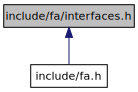
\includegraphics[width=350pt]{interfaces_8h__dep__incl}
\end{center}
\end{figure}
\subsection*{Enumerations}
\begin{DoxyCompactItemize}
\item 
enum \hyperlink{interfaces_8h_a7c337b4de759549a84c656770ce01cd2}{fa\-\_\-interfaces} \{ \\*
\hyperlink{interfaces_8h_a7c337b4de759549a84c656770ce01cd2a6c72433711c948606edc4a0327023a56}{fa\-\_\-copy\-\_\-i}, 
\hyperlink{interfaces_8h_a7c337b4de759549a84c656770ce01cd2a15b9f6db28aa00dad20e0537ebd68e8e}{fa\-\_\-destroy\-\_\-i}, 
\hyperlink{interfaces_8h_a7c337b4de759549a84c656770ce01cd2ad4d9c8c03152cbc55596505182479239}{fa\-\_\-dynamic\-\_\-i}, 
\hyperlink{interfaces_8h_a7c337b4de759549a84c656770ce01cd2aa3e8efbadb2c2678959576a6e2346dfc}{fa\-\_\-error\-\_\-i}, 
\\*
\hyperlink{interfaces_8h_a7c337b4de759549a84c656770ce01cd2a9b8bb278c9a713e6ec54d275002e0a01}{fa\-\_\-equal\-\_\-i}, 
\hyperlink{interfaces_8h_a7c337b4de759549a84c656770ce01cd2ae08a92558a44d2796dc2a5df8ff1b3c3}{fa\-\_\-order\-\_\-i}, 
\hyperlink{interfaces_8h_a7c337b4de759549a84c656770ce01cd2a29a648811f9c4772b419decc4b00048b}{fa\-\_\-number\-\_\-i}, 
\hyperlink{interfaces_8h_a7c337b4de759549a84c656770ce01cd2ae3047dcd8bdee218a2c19fc3e7543729}{fa\-\_\-clock\-\_\-interface\-\_\-i}, 
\\*
\hyperlink{interfaces_8h_a7c337b4de759549a84c656770ce01cd2aee17a8c8a2a5ba11a7c8b35e5765ea40}{fa\-\_\-io\-\_\-filter\-\_\-interface\-\_\-i}, 
\hyperlink{interfaces_8h_a7c337b4de759549a84c656770ce01cd2a288b4ff774c44b5d4915d2337fea1307}{fa\-\_\-string\-\_\-show\-\_\-i}
 \}
\end{DoxyCompactItemize}


\subsection{Enumeration Type Documentation}
\hypertarget{interfaces_8h_a7c337b4de759549a84c656770ce01cd2}{\index{interfaces.\-h@{interfaces.\-h}!fa\-\_\-interfaces@{fa\-\_\-interfaces}}
\index{fa\-\_\-interfaces@{fa\-\_\-interfaces}!interfaces.h@{interfaces.\-h}}
\subsubsection[{fa\-\_\-interfaces}]{\setlength{\rightskip}{0pt plus 5cm}enum {\bf fa\-\_\-interfaces}}}\label{interfaces_8h_a7c337b4de759549a84c656770ce01cd2}
\begin{Desc}
\item[Enumerator]\par
\begin{description}
\index{fa\-\_\-copy\-\_\-i@{fa\-\_\-copy\-\_\-i}!interfaces.\-h@{interfaces.\-h}}\index{interfaces.\-h@{interfaces.\-h}!fa\-\_\-copy\-\_\-i@{fa\-\_\-copy\-\_\-i}}\item[{\em 
\hypertarget{interfaces_8h_a7c337b4de759549a84c656770ce01cd2a6c72433711c948606edc4a0327023a56}{fa\-\_\-copy\-\_\-i}\label{interfaces_8h_a7c337b4de759549a84c656770ce01cd2a6c72433711c948606edc4a0327023a56}
}]\index{fa\-\_\-destroy\-\_\-i@{fa\-\_\-destroy\-\_\-i}!interfaces.\-h@{interfaces.\-h}}\index{interfaces.\-h@{interfaces.\-h}!fa\-\_\-destroy\-\_\-i@{fa\-\_\-destroy\-\_\-i}}\item[{\em 
\hypertarget{interfaces_8h_a7c337b4de759549a84c656770ce01cd2a15b9f6db28aa00dad20e0537ebd68e8e}{fa\-\_\-destroy\-\_\-i}\label{interfaces_8h_a7c337b4de759549a84c656770ce01cd2a15b9f6db28aa00dad20e0537ebd68e8e}
}]\index{fa\-\_\-dynamic\-\_\-i@{fa\-\_\-dynamic\-\_\-i}!interfaces.\-h@{interfaces.\-h}}\index{interfaces.\-h@{interfaces.\-h}!fa\-\_\-dynamic\-\_\-i@{fa\-\_\-dynamic\-\_\-i}}\item[{\em 
\hypertarget{interfaces_8h_a7c337b4de759549a84c656770ce01cd2ad4d9c8c03152cbc55596505182479239}{fa\-\_\-dynamic\-\_\-i}\label{interfaces_8h_a7c337b4de759549a84c656770ce01cd2ad4d9c8c03152cbc55596505182479239}
}]\index{fa\-\_\-error\-\_\-i@{fa\-\_\-error\-\_\-i}!interfaces.\-h@{interfaces.\-h}}\index{interfaces.\-h@{interfaces.\-h}!fa\-\_\-error\-\_\-i@{fa\-\_\-error\-\_\-i}}\item[{\em 
\hypertarget{interfaces_8h_a7c337b4de759549a84c656770ce01cd2aa3e8efbadb2c2678959576a6e2346dfc}{fa\-\_\-error\-\_\-i}\label{interfaces_8h_a7c337b4de759549a84c656770ce01cd2aa3e8efbadb2c2678959576a6e2346dfc}
}]\index{fa\-\_\-equal\-\_\-i@{fa\-\_\-equal\-\_\-i}!interfaces.\-h@{interfaces.\-h}}\index{interfaces.\-h@{interfaces.\-h}!fa\-\_\-equal\-\_\-i@{fa\-\_\-equal\-\_\-i}}\item[{\em 
\hypertarget{interfaces_8h_a7c337b4de759549a84c656770ce01cd2a9b8bb278c9a713e6ec54d275002e0a01}{fa\-\_\-equal\-\_\-i}\label{interfaces_8h_a7c337b4de759549a84c656770ce01cd2a9b8bb278c9a713e6ec54d275002e0a01}
}]\index{fa\-\_\-order\-\_\-i@{fa\-\_\-order\-\_\-i}!interfaces.\-h@{interfaces.\-h}}\index{interfaces.\-h@{interfaces.\-h}!fa\-\_\-order\-\_\-i@{fa\-\_\-order\-\_\-i}}\item[{\em 
\hypertarget{interfaces_8h_a7c337b4de759549a84c656770ce01cd2ae08a92558a44d2796dc2a5df8ff1b3c3}{fa\-\_\-order\-\_\-i}\label{interfaces_8h_a7c337b4de759549a84c656770ce01cd2ae08a92558a44d2796dc2a5df8ff1b3c3}
}]\index{fa\-\_\-number\-\_\-i@{fa\-\_\-number\-\_\-i}!interfaces.\-h@{interfaces.\-h}}\index{interfaces.\-h@{interfaces.\-h}!fa\-\_\-number\-\_\-i@{fa\-\_\-number\-\_\-i}}\item[{\em 
\hypertarget{interfaces_8h_a7c337b4de759549a84c656770ce01cd2a29a648811f9c4772b419decc4b00048b}{fa\-\_\-number\-\_\-i}\label{interfaces_8h_a7c337b4de759549a84c656770ce01cd2a29a648811f9c4772b419decc4b00048b}
}]\index{fa\-\_\-clock\-\_\-interface\-\_\-i@{fa\-\_\-clock\-\_\-interface\-\_\-i}!interfaces.\-h@{interfaces.\-h}}\index{interfaces.\-h@{interfaces.\-h}!fa\-\_\-clock\-\_\-interface\-\_\-i@{fa\-\_\-clock\-\_\-interface\-\_\-i}}\item[{\em 
\hypertarget{interfaces_8h_a7c337b4de759549a84c656770ce01cd2ae3047dcd8bdee218a2c19fc3e7543729}{fa\-\_\-clock\-\_\-interface\-\_\-i}\label{interfaces_8h_a7c337b4de759549a84c656770ce01cd2ae3047dcd8bdee218a2c19fc3e7543729}
}]\index{fa\-\_\-io\-\_\-filter\-\_\-interface\-\_\-i@{fa\-\_\-io\-\_\-filter\-\_\-interface\-\_\-i}!interfaces.\-h@{interfaces.\-h}}\index{interfaces.\-h@{interfaces.\-h}!fa\-\_\-io\-\_\-filter\-\_\-interface\-\_\-i@{fa\-\_\-io\-\_\-filter\-\_\-interface\-\_\-i}}\item[{\em 
\hypertarget{interfaces_8h_a7c337b4de759549a84c656770ce01cd2aee17a8c8a2a5ba11a7c8b35e5765ea40}{fa\-\_\-io\-\_\-filter\-\_\-interface\-\_\-i}\label{interfaces_8h_a7c337b4de759549a84c656770ce01cd2aee17a8c8a2a5ba11a7c8b35e5765ea40}
}]\index{fa\-\_\-string\-\_\-show\-\_\-i@{fa\-\_\-string\-\_\-show\-\_\-i}!interfaces.\-h@{interfaces.\-h}}\index{interfaces.\-h@{interfaces.\-h}!fa\-\_\-string\-\_\-show\-\_\-i@{fa\-\_\-string\-\_\-show\-\_\-i}}\item[{\em 
\hypertarget{interfaces_8h_a7c337b4de759549a84c656770ce01cd2a288b4ff774c44b5d4915d2337fea1307}{fa\-\_\-string\-\_\-show\-\_\-i}\label{interfaces_8h_a7c337b4de759549a84c656770ce01cd2a288b4ff774c44b5d4915d2337fea1307}
}]\end{description}
\end{Desc}

\hypertarget{io_8h}{\section{include/fa/io.h File Reference}
\label{io_8h}\index{include/fa/io.\-h@{include/fa/io.\-h}}
}
{\ttfamily \#include $<$fa.\-h$>$}\\*
{\ttfamily \#include $<$fa/buffer.\-h$>$}\\*
{\ttfamily \#include $<$fa/atomic/ring\-\_\-buffer.\-h$>$}\\*
Include dependency graph for io.\-h\-:\nopagebreak
\begin{figure}[H]
\begin{center}
\leavevmode
\includegraphics[width=350pt]{io_8h__incl}
\end{center}
\end{figure}
\subsection*{Data Structures}
\begin{DoxyCompactItemize}
\item 
struct \hyperlink{structfa__io__filter__interface__t}{fa\-\_\-io\-\_\-filter\-\_\-interface\-\_\-t}
\end{DoxyCompactItemize}
\subsection*{Typedefs}
\begin{DoxyCompactItemize}
\item 
typedef void($\ast$ \hyperlink{group___fa_io_gaa151f2c484756349795513fdf67a0268}{fa\-\_\-io\-\_\-callback\-\_\-t} )(\hyperlink{group___fa_ga915ddeae99ad7568b273d2b876425197}{fa\-\_\-ptr\-\_\-t}, \hyperlink{group___fa_buffer_ga0ed7a1d783ab322e2e8be02432d0839e}{fa\-\_\-buffer\-\_\-t})
\begin{DoxyCompactList}\small\item\em Callback to receive data. \end{DoxyCompactList}\item 
typedef void($\ast$ \hyperlink{group___fa_io_gabadf768f91c382d0700638f384f48416}{fa\-\_\-io\-\_\-read\-\_\-callback\-\_\-t} )(\hyperlink{group___fa_ga915ddeae99ad7568b273d2b876425197}{fa\-\_\-ptr\-\_\-t}, \hyperlink{group___fa_io_gaa151f2c484756349795513fdf67a0268}{fa\-\_\-io\-\_\-callback\-\_\-t}, \hyperlink{group___fa_ga915ddeae99ad7568b273d2b876425197}{fa\-\_\-ptr\-\_\-t})
\begin{DoxyCompactList}\small\item\em Callback to recive callback to receive data. \end{DoxyCompactList}\item 
typedef struct \-\_\-fa\-\_\-io\-\_\-filter\-\_\-t $\ast$ \hyperlink{group___fa_io_ga3e1f11810efcba3b45842e10c1425aba}{fa\-\_\-io\-\_\-filter\-\_\-t}
\begin{DoxyCompactList}\small\item\em Implements the filter interface. \end{DoxyCompactList}\item 
typedef struct \-\_\-fa\-\_\-io\-\_\-source\-\_\-t $\ast$ \hyperlink{group___fa_io_ga95a53a87c83414434e1afd3097b96ea4}{fa\-\_\-io\-\_\-source\-\_\-t}
\begin{DoxyCompactList}\small\item\em Implements the filter interface (push calls have no effect, pull ignores the source). \end{DoxyCompactList}\item 
typedef struct \-\_\-fa\-\_\-io\-\_\-sink\-\_\-t $\ast$ \hyperlink{group___fa_io_ga0d00d1e2c742abdba97597662815ce3a}{fa\-\_\-io\-\_\-sink\-\_\-t}
\begin{DoxyCompactList}\small\item\em Implements the filter interface (pull calls have no effect, push ignores the sink). \end{DoxyCompactList}\end{DoxyCompactItemize}
\subsection*{Functions}
\begin{DoxyCompactItemize}
\item 
void \hyperlink{group___fa_io_ga3d6948a08503213c1c48beab1938e7b1}{fa\-\_\-io\-\_\-pull} (\hyperlink{group___fa_io_ga95a53a87c83414434e1afd3097b96ea4}{fa\-\_\-io\-\_\-source\-\_\-t} source, \hyperlink{group___fa_io_gaa151f2c484756349795513fdf67a0268}{fa\-\_\-io\-\_\-callback\-\_\-t} callback, \hyperlink{group___fa_ga915ddeae99ad7568b273d2b876425197}{fa\-\_\-ptr\-\_\-t} ptr)
\begin{DoxyCompactList}\small\item\em Pull data from a source. \end{DoxyCompactList}\item 
void \hyperlink{group___fa_io_ga37b29056c1f719c9a4d4cd1ef11e2584}{fa\-\_\-io\-\_\-push} (\hyperlink{group___fa_io_ga0d00d1e2c742abdba97597662815ce3a}{fa\-\_\-io\-\_\-sink\-\_\-t} sink, \hyperlink{group___fa_buffer_ga0ed7a1d783ab322e2e8be02432d0839e}{fa\-\_\-buffer\-\_\-t} \hyperlink{util_8h_ad0c623e8b04565926f5b48888327724a}{buffer})
\begin{DoxyCompactList}\small\item\em Push data to a sink. \end{DoxyCompactList}\item 
void \hyperlink{group___fa_io_ga249b3427c89eaf4fff61ea26582c6977}{fa\-\_\-io\-\_\-pull\-\_\-through} (\hyperlink{group___fa_io_ga3e1f11810efcba3b45842e10c1425aba}{fa\-\_\-io\-\_\-filter\-\_\-t} filter, \hyperlink{group___fa_io_ga95a53a87c83414434e1afd3097b96ea4}{fa\-\_\-io\-\_\-source\-\_\-t} source, \hyperlink{group___fa_io_gaa151f2c484756349795513fdf67a0268}{fa\-\_\-io\-\_\-callback\-\_\-t} callback, \hyperlink{group___fa_ga915ddeae99ad7568b273d2b876425197}{fa\-\_\-ptr\-\_\-t} ptr)
\begin{DoxyCompactList}\small\item\em Pull data from a source after passing it through the given filter. \end{DoxyCompactList}\item 
void \hyperlink{group___fa_io_ga468831a94c4cdda4769a09a92fcae3ca}{fa\-\_\-io\-\_\-push\-\_\-through} (\hyperlink{group___fa_io_ga3e1f11810efcba3b45842e10c1425aba}{fa\-\_\-io\-\_\-filter\-\_\-t} filter, \hyperlink{group___fa_io_ga0d00d1e2c742abdba97597662815ce3a}{fa\-\_\-io\-\_\-sink\-\_\-t} sink, \hyperlink{group___fa_buffer_ga0ed7a1d783ab322e2e8be02432d0839e}{fa\-\_\-buffer\-\_\-t} \hyperlink{util_8h_ad0c623e8b04565926f5b48888327724a}{buffer})
\begin{DoxyCompactList}\small\item\em Push data to a sink after passing it through the given filter. \end{DoxyCompactList}\item 
\hyperlink{group___fa_io_ga3e1f11810efcba3b45842e10c1425aba}{fa\-\_\-io\-\_\-filter\-\_\-t} \hyperlink{group___fa_io_gab9e18903ead86c8e6c2cdd190b6412ab}{fa\-\_\-io\-\_\-identity} ()
\begin{DoxyCompactList}\small\item\em Create filter that passes through its input unchanged. \end{DoxyCompactList}\item 
\hyperlink{group___fa_io_ga3e1f11810efcba3b45842e10c1425aba}{fa\-\_\-io\-\_\-filter\-\_\-t} \hyperlink{group___fa_io_gabeb62824d4c0ce4f45b6c901e7aca3ac}{fa\-\_\-io\-\_\-compose} (\hyperlink{group___fa_io_ga3e1f11810efcba3b45842e10c1425aba}{fa\-\_\-io\-\_\-filter\-\_\-t} filter, \hyperlink{group___fa_io_ga3e1f11810efcba3b45842e10c1425aba}{fa\-\_\-io\-\_\-filter\-\_\-t} filter\-\_\-)
\begin{DoxyCompactList}\small\item\em Compose two filters. \end{DoxyCompactList}\item 
\hyperlink{group___fa_io_ga95a53a87c83414434e1afd3097b96ea4}{fa\-\_\-io\-\_\-source\-\_\-t} \hyperlink{group___fa_io_ga1217e66827a628653d8386805039f1d3}{fa\-\_\-io\-\_\-apply} (\hyperlink{group___fa_io_ga95a53a87c83414434e1afd3097b96ea4}{fa\-\_\-io\-\_\-source\-\_\-t} source, \hyperlink{group___fa_io_ga3e1f11810efcba3b45842e10c1425aba}{fa\-\_\-io\-\_\-filter\-\_\-t} filter)
\begin{DoxyCompactList}\small\item\em Apply a filter to the output of a source. \end{DoxyCompactList}\item 
\hyperlink{group___fa_io_ga0d00d1e2c742abdba97597662815ce3a}{fa\-\_\-io\-\_\-sink\-\_\-t} \hyperlink{group___fa_io_ga0b81abcccb362aac530ce0c5be30068f}{fa\-\_\-io\-\_\-coapply} (\hyperlink{group___fa_io_ga3e1f11810efcba3b45842e10c1425aba}{fa\-\_\-io\-\_\-filter\-\_\-t} filter, \hyperlink{group___fa_io_ga0d00d1e2c742abdba97597662815ce3a}{fa\-\_\-io\-\_\-sink\-\_\-t} sink)
\begin{DoxyCompactList}\small\item\em Apply a filter to the input of a sink. \end{DoxyCompactList}\item 
\hyperlink{group___fa_io_ga3e1f11810efcba3b45842e10c1425aba}{fa\-\_\-io\-\_\-filter\-\_\-t} \hyperlink{group___fa_io_ga0f2da1ffcf02190f82e3b20583b2c340}{fa\-\_\-io\-\_\-create\-\_\-simple\-\_\-filter} (\hyperlink{group___fa_io_gaa151f2c484756349795513fdf67a0268}{fa\-\_\-io\-\_\-callback\-\_\-t} callback, \hyperlink{group___fa_io_gabadf768f91c382d0700638f384f48416}{fa\-\_\-io\-\_\-read\-\_\-callback\-\_\-t} read\-Callback, \hyperlink{group___fa_ga915ddeae99ad7568b273d2b876425197}{fa\-\_\-ptr\-\_\-t} ptr)
\begin{DoxyCompactList}\small\item\em Create a simple stateful filter. \end{DoxyCompactList}\item 
\hyperlink{group___fa_io_ga3e1f11810efcba3b45842e10c1425aba}{fa\-\_\-io\-\_\-filter\-\_\-t} \hyperlink{group___fa_io_ga2c8a8774e54c943b9972c18333971978}{fa\-\_\-io\-\_\-split} (\hyperlink{group___fa_io_ga0d00d1e2c742abdba97597662815ce3a}{fa\-\_\-io\-\_\-sink\-\_\-t} sink)
\begin{DoxyCompactList}\small\item\em Create a filter that writes data passed through it to the given sink. \end{DoxyCompactList}\item 
\hyperlink{group___fa_io_ga95a53a87c83414434e1afd3097b96ea4}{fa\-\_\-io\-\_\-source\-\_\-t} \hyperlink{group___fa_io_ga2d7dd21d610308d507d2471236e426b5}{fa\-\_\-io\-\_\-read\-\_\-file} (\hyperlink{group___fa_string_gacada63033b77bc6c39fa632ae199349b}{fa\-\_\-string\-\_\-t} \hyperlink{util_8h_a41106000aac73b61e4fc2ef9dd39a603}{string})
\begin{DoxyCompactList}\small\item\em Create source that reads from a file. \end{DoxyCompactList}\item 
\hyperlink{group___fa_io_ga0d00d1e2c742abdba97597662815ce3a}{fa\-\_\-io\-\_\-sink\-\_\-t} \hyperlink{group___fa_io_ga6c55c0dff1d5e8fca3ec227b66beddcb}{fa\-\_\-io\-\_\-write\-\_\-file} (\hyperlink{group___fa_string_gacada63033b77bc6c39fa632ae199349b}{fa\-\_\-string\-\_\-t} \hyperlink{util_8h_a41106000aac73b61e4fc2ef9dd39a603}{string})
\begin{DoxyCompactList}\small\item\em Create source that writes to a file. \end{DoxyCompactList}\item 
\hyperlink{group___fa_io_ga95a53a87c83414434e1afd3097b96ea4}{fa\-\_\-io\-\_\-source\-\_\-t} \hyperlink{group___fa_io_gafea99482db8d693d53d6b157960e06af}{fa\-\_\-io\-\_\-standard\-\_\-in} ()
\begin{DoxyCompactList}\small\item\em Create source that reads from the standard input. \end{DoxyCompactList}\item 
\hyperlink{group___fa_io_ga0d00d1e2c742abdba97597662815ce3a}{fa\-\_\-io\-\_\-sink\-\_\-t} \hyperlink{group___fa_io_ga8cd0d250bdd1193a418df62a7f0f7bb8}{fa\-\_\-io\-\_\-standard\-\_\-out} ()
\begin{DoxyCompactList}\small\item\em Create source that reads to the standard output. \end{DoxyCompactList}\item 
\hyperlink{group___fa_io_ga95a53a87c83414434e1afd3097b96ea4}{fa\-\_\-io\-\_\-source\-\_\-t} \hyperlink{group___fa_io_ga7fc84d8c573c3a2b7e6a7eb04d399634}{fa\-\_\-io\-\_\-from\-\_\-ring\-\_\-buffer} (\hyperlink{group___fa_atomic_ring_buffer_ga3482421740e66f489d94407a0d48a2d0}{fa\-\_\-atomic\-\_\-ring\-\_\-buffer\-\_\-t} ring\-Buffer)
\begin{DoxyCompactList}\small\item\em Create a source from a ring buffer. \end{DoxyCompactList}\item 
\hyperlink{group___fa_io_ga3e1f11810efcba3b45842e10c1425aba}{fa\-\_\-io\-\_\-filter\-\_\-t} \hyperlink{group___fa_io_ga3b642b72902c40600b387cf6097f01f7}{fa\-\_\-io\-\_\-create\-\_\-ogg\-\_\-encoder} ()
\begin{DoxyCompactList}\small\item\em Create an encoder to the {\ttfamily ogg/vorbis} format. \end{DoxyCompactList}\item 
void \hyperlink{group___fa_io_ga358e5b87997d711d52e841222c2eab5d}{fa\-\_\-io\-\_\-run} (\hyperlink{group___fa_io_ga95a53a87c83414434e1afd3097b96ea4}{fa\-\_\-io\-\_\-source\-\_\-t} source, \hyperlink{group___fa_io_ga0d00d1e2c742abdba97597662815ce3a}{fa\-\_\-io\-\_\-sink\-\_\-t} sink)
\begin{DoxyCompactList}\small\item\em Continously data from the given source and push it into the sink. \end{DoxyCompactList}\end{DoxyCompactItemize}

\hypertarget{list_8h}{\section{include/fa/list.h File Reference}
\label{list_8h}\index{include/fa/list.\-h@{include/fa/list.\-h}}
}
{\ttfamily \#include $<$fa.\-h$>$}\\*
Include dependency graph for list.\-h\-:\nopagebreak
\begin{figure}[H]
\begin{center}
\leavevmode
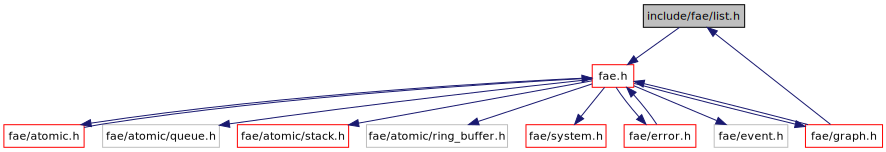
\includegraphics[width=350pt]{list_8h__incl}
\end{center}
\end{figure}
This graph shows which files directly or indirectly include this file\-:\nopagebreak
\begin{figure}[H]
\begin{center}
\leavevmode
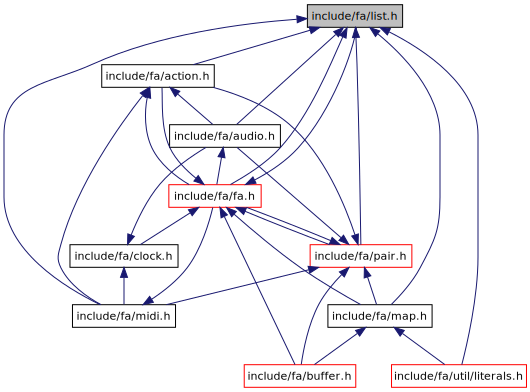
\includegraphics[width=350pt]{list_8h__dep__incl}
\end{center}
\end{figure}
\subsection*{Typedefs}
\begin{DoxyCompactItemize}
\item 
typedef struct \-\_\-fa\-\_\-list\-\_\-t $\ast$ \hyperlink{group___fa_list_ga35ecb12ab934ded0cce0bcf28e3bc5d2}{fa\-\_\-list\-\_\-t}
\end{DoxyCompactItemize}
\subsection*{Functions}
\begin{DoxyCompactItemize}
\item 
\hyperlink{group___fa_list_ga35ecb12ab934ded0cce0bcf28e3bc5d2}{fa\-\_\-list\-\_\-t} \hyperlink{group___fa_list_gabf678944a2862ba07072920e37cdb23d}{fa\-\_\-list\-\_\-empty} ()
\begin{DoxyCompactList}\small\item\em Create an empty list. \end{DoxyCompactList}\item 
\hyperlink{group___fa_list_ga35ecb12ab934ded0cce0bcf28e3bc5d2}{fa\-\_\-list\-\_\-t} \hyperlink{group___fa_list_ga69d1eb03989a1f8349c292ceed66fd6a}{fa\-\_\-list\-\_\-single} (\hyperlink{group___fa_ga915ddeae99ad7568b273d2b876425197}{fa\-\_\-ptr\-\_\-t} ptr)
\begin{DoxyCompactList}\small\item\em Create a new list containing the given element. \end{DoxyCompactList}\item 
\hyperlink{group___fa_list_ga35ecb12ab934ded0cce0bcf28e3bc5d2}{fa\-\_\-list\-\_\-t} \hyperlink{group___fa_list_ga3cff1dce5051c7e1dd9ef255be911204}{fa\-\_\-list\-\_\-cons} (\hyperlink{group___fa_ga915ddeae99ad7568b273d2b876425197}{fa\-\_\-ptr\-\_\-t} ptr, \hyperlink{group___fa_list_ga35ecb12ab934ded0cce0bcf28e3bc5d2}{fa\-\_\-list\-\_\-t} \hyperlink{literals_8h_a4ddd63dfcfec2b4d5741a56aa6003c76}{list})
\begin{DoxyCompactList}\small\item\em Create a new list by inserting the given element at the beginning of the given list. \end{DoxyCompactList}\item 
\hyperlink{group___fa_list_ga35ecb12ab934ded0cce0bcf28e3bc5d2}{fa\-\_\-list\-\_\-t} \hyperlink{group___fa_list_ga29aba2e79fd9c128c05d020be5a3b254}{fa\-\_\-list\-\_\-dcons} (\hyperlink{group___fa_ga915ddeae99ad7568b273d2b876425197}{fa\-\_\-ptr\-\_\-t} ptr, \hyperlink{group___fa_list_ga35ecb12ab934ded0cce0bcf28e3bc5d2}{fa\-\_\-list\-\_\-t} \hyperlink{literals_8h_a4ddd63dfcfec2b4d5741a56aa6003c76}{list})
\begin{DoxyCompactList}\small\item\em Create a new list by inserting the given element at the beginning of the given list. \end{DoxyCompactList}\item 
\hyperlink{group___fa_list_ga35ecb12ab934ded0cce0bcf28e3bc5d2}{fa\-\_\-list\-\_\-t} \hyperlink{group___fa_list_gacadd05a228af713c5fe13c5baf09ce84}{fa\-\_\-list\-\_\-repeat} (int int\-\_\-, \hyperlink{group___fa_ga915ddeae99ad7568b273d2b876425197}{fa\-\_\-ptr\-\_\-t} ptr)
\begin{DoxyCompactList}\small\item\em Create a list by repeating the given element. \end{DoxyCompactList}\item 
\hyperlink{group___fa_list_ga35ecb12ab934ded0cce0bcf28e3bc5d2}{fa\-\_\-list\-\_\-t} \hyperlink{group___fa_list_ga032f7d2288130530305801146e76093c}{fa\-\_\-list\-\_\-enumerate} (int int\-\_\-, int int\-\_\-\-\_\-)
\begin{DoxyCompactList}\small\item\em Create a list from the given range. \end{DoxyCompactList}\item 
\hyperlink{group___fa_list_ga35ecb12ab934ded0cce0bcf28e3bc5d2}{fa\-\_\-list\-\_\-t} \hyperlink{group___fa_list_ga21ddfd967b94ffb34215a74de16fe106}{fa\-\_\-list\-\_\-copy} (\hyperlink{group___fa_list_ga35ecb12ab934ded0cce0bcf28e3bc5d2}{fa\-\_\-list\-\_\-t} \hyperlink{literals_8h_a4ddd63dfcfec2b4d5741a56aa6003c76}{list})
\begin{DoxyCompactList}\small\item\em Copy the given list. \end{DoxyCompactList}\item 
void \hyperlink{group___fa_list_gafbf19f83b9ea6896be97f5bf572d61ad}{fa\-\_\-list\-\_\-destroy} (\hyperlink{group___fa_list_ga35ecb12ab934ded0cce0bcf28e3bc5d2}{fa\-\_\-list\-\_\-t} \hyperlink{literals_8h_a4ddd63dfcfec2b4d5741a56aa6003c76}{list})
\begin{DoxyCompactList}\small\item\em Destroy the given list. \end{DoxyCompactList}\item 
bool \hyperlink{group___fa_list_ga094f7dda2ad993812f47804f4d68dfaa}{fa\-\_\-list\-\_\-is\-\_\-empty} (\hyperlink{group___fa_list_ga35ecb12ab934ded0cce0bcf28e3bc5d2}{fa\-\_\-list\-\_\-t} \hyperlink{literals_8h_a4ddd63dfcfec2b4d5741a56aa6003c76}{list})
\begin{DoxyCompactList}\small\item\em Return whether the given list is empty. \end{DoxyCompactList}\item 
bool \hyperlink{group___fa_list_gab7cd6228e5a29b4e07ec65c5e35780d0}{fa\-\_\-list\-\_\-is\-\_\-single} (\hyperlink{group___fa_list_ga35ecb12ab934ded0cce0bcf28e3bc5d2}{fa\-\_\-list\-\_\-t} \hyperlink{literals_8h_a4ddd63dfcfec2b4d5741a56aa6003c76}{list})
\begin{DoxyCompactList}\small\item\em Return whether the given list has a single element. \end{DoxyCompactList}\item 
int \hyperlink{group___fa_list_ga3c752b5fff701e2b8e40d68ca6197350}{fa\-\_\-list\-\_\-length} (\hyperlink{group___fa_list_ga35ecb12ab934ded0cce0bcf28e3bc5d2}{fa\-\_\-list\-\_\-t} \hyperlink{literals_8h_a4ddd63dfcfec2b4d5741a56aa6003c76}{list})
\begin{DoxyCompactList}\small\item\em Return the lenght of the given list. \end{DoxyCompactList}\item 
\hyperlink{group___fa_ga915ddeae99ad7568b273d2b876425197}{fa\-\_\-ptr\-\_\-t} \hyperlink{group___fa_list_ga1a631bffa52d40cd55e7b92dce3ad9c4}{fa\-\_\-list\-\_\-head} (\hyperlink{group___fa_list_ga35ecb12ab934ded0cce0bcf28e3bc5d2}{fa\-\_\-list\-\_\-t} \hyperlink{literals_8h_a4ddd63dfcfec2b4d5741a56aa6003c76}{list})
\begin{DoxyCompactList}\small\item\em Return the first element of the given list. \end{DoxyCompactList}\item 
\hyperlink{group___fa_list_ga35ecb12ab934ded0cce0bcf28e3bc5d2}{fa\-\_\-list\-\_\-t} \hyperlink{group___fa_list_gac93acb3b5b61ccdacfe2680b6d56c286}{fa\-\_\-list\-\_\-tail} (\hyperlink{group___fa_list_ga35ecb12ab934ded0cce0bcf28e3bc5d2}{fa\-\_\-list\-\_\-t} \hyperlink{literals_8h_a4ddd63dfcfec2b4d5741a56aa6003c76}{list})
\begin{DoxyCompactList}\small\item\em Return all elements but the first of the given list. \end{DoxyCompactList}\item 
\hyperlink{group___fa_list_ga35ecb12ab934ded0cce0bcf28e3bc5d2}{fa\-\_\-list\-\_\-t} \hyperlink{group___fa_list_ga20497863c1110218c0f184ec23f960a0}{fa\-\_\-list\-\_\-dtail} (\hyperlink{group___fa_list_ga35ecb12ab934ded0cce0bcf28e3bc5d2}{fa\-\_\-list\-\_\-t} \hyperlink{literals_8h_a4ddd63dfcfec2b4d5741a56aa6003c76}{list})
\begin{DoxyCompactList}\small\item\em Return all elements but the first of the given list. \end{DoxyCompactList}\item 
\hyperlink{group___fa_list_ga35ecb12ab934ded0cce0bcf28e3bc5d2}{fa\-\_\-list\-\_\-t} \hyperlink{group___fa_list_ga32a54ff3c9f7d1741d41e6e0155e960b}{fa\-\_\-list\-\_\-init} (\hyperlink{group___fa_list_ga35ecb12ab934ded0cce0bcf28e3bc5d2}{fa\-\_\-list\-\_\-t} \hyperlink{literals_8h_a4ddd63dfcfec2b4d5741a56aa6003c76}{list})
\begin{DoxyCompactList}\small\item\em Return all elements but the last of the given list. \end{DoxyCompactList}\item 
\hyperlink{group___fa_list_ga35ecb12ab934ded0cce0bcf28e3bc5d2}{fa\-\_\-list\-\_\-t} \hyperlink{group___fa_list_ga79588d4812728fcfd260d37c2eed38a5}{fa\-\_\-list\-\_\-dinit} (\hyperlink{group___fa_list_ga35ecb12ab934ded0cce0bcf28e3bc5d2}{fa\-\_\-list\-\_\-t} \hyperlink{literals_8h_a4ddd63dfcfec2b4d5741a56aa6003c76}{list})
\begin{DoxyCompactList}\small\item\em Return all elements but the last of the given list. \end{DoxyCompactList}\item 
\hyperlink{group___fa_ga915ddeae99ad7568b273d2b876425197}{fa\-\_\-ptr\-\_\-t} \hyperlink{group___fa_list_ga8e381af7983cac00ff95ad1f468dd90a}{fa\-\_\-list\-\_\-last} (\hyperlink{group___fa_list_ga35ecb12ab934ded0cce0bcf28e3bc5d2}{fa\-\_\-list\-\_\-t} \hyperlink{literals_8h_a4ddd63dfcfec2b4d5741a56aa6003c76}{list})
\begin{DoxyCompactList}\small\item\em Return the last element of the given list. \end{DoxyCompactList}\item 
\hyperlink{group___fa_list_ga35ecb12ab934ded0cce0bcf28e3bc5d2}{fa\-\_\-list\-\_\-t} \hyperlink{group___fa_list_ga5c51602ab144ef57ec504d2128066992}{fa\-\_\-list\-\_\-append} (\hyperlink{group___fa_list_ga35ecb12ab934ded0cce0bcf28e3bc5d2}{fa\-\_\-list\-\_\-t} \hyperlink{literals_8h_a4ddd63dfcfec2b4d5741a56aa6003c76}{list}, \hyperlink{group___fa_list_ga35ecb12ab934ded0cce0bcf28e3bc5d2}{fa\-\_\-list\-\_\-t} list\-\_\-)
\begin{DoxyCompactList}\small\item\em Return the result of appending the given lists. \end{DoxyCompactList}\item 
\hyperlink{group___fa_list_ga35ecb12ab934ded0cce0bcf28e3bc5d2}{fa\-\_\-list\-\_\-t} \hyperlink{group___fa_list_gae17a6b6ead9c469d08f19c1a80746462}{fa\-\_\-list\-\_\-dappend} (\hyperlink{group___fa_list_ga35ecb12ab934ded0cce0bcf28e3bc5d2}{fa\-\_\-list\-\_\-t} \hyperlink{literals_8h_a4ddd63dfcfec2b4d5741a56aa6003c76}{list}, \hyperlink{group___fa_list_ga35ecb12ab934ded0cce0bcf28e3bc5d2}{fa\-\_\-list\-\_\-t} list\-\_\-)
\begin{DoxyCompactList}\small\item\em Return the result of appending the given lists. \end{DoxyCompactList}\item 
\hyperlink{group___fa_list_ga35ecb12ab934ded0cce0bcf28e3bc5d2}{fa\-\_\-list\-\_\-t} \hyperlink{group___fa_list_ga7b187ef70819a17992b0d787683de241}{fa\-\_\-list\-\_\-reverse} (\hyperlink{group___fa_list_ga35ecb12ab934ded0cce0bcf28e3bc5d2}{fa\-\_\-list\-\_\-t} \hyperlink{literals_8h_a4ddd63dfcfec2b4d5741a56aa6003c76}{list})
\begin{DoxyCompactList}\small\item\em Return the reverse of the given list. \end{DoxyCompactList}\item 
\hyperlink{group___fa_list_ga35ecb12ab934ded0cce0bcf28e3bc5d2}{fa\-\_\-list\-\_\-t} \hyperlink{group___fa_list_gab949bb4c4f8c373aeddb98fbc3398245}{fa\-\_\-list\-\_\-dreverse} (\hyperlink{group___fa_list_ga35ecb12ab934ded0cce0bcf28e3bc5d2}{fa\-\_\-list\-\_\-t} \hyperlink{literals_8h_a4ddd63dfcfec2b4d5741a56aa6003c76}{list})
\begin{DoxyCompactList}\small\item\em Return the reverse of the given list. \end{DoxyCompactList}\item 
\hyperlink{group___fa_list_ga35ecb12ab934ded0cce0bcf28e3bc5d2}{fa\-\_\-list\-\_\-t} \hyperlink{group___fa_list_gaf80f08f28121092f5afb04c66a0ce086}{fa\-\_\-list\-\_\-sort} (\hyperlink{group___fa_list_ga35ecb12ab934ded0cce0bcf28e3bc5d2}{fa\-\_\-list\-\_\-t} \hyperlink{literals_8h_a4ddd63dfcfec2b4d5741a56aa6003c76}{list})
\begin{DoxyCompactList}\small\item\em Return the given list sorted. \end{DoxyCompactList}\item 
\hyperlink{group___fa_list_ga35ecb12ab934ded0cce0bcf28e3bc5d2}{fa\-\_\-list\-\_\-t} \hyperlink{group___fa_list_ga9f51ef4df289a25cec79bbcdb995cbaa}{fa\-\_\-list\-\_\-dsort} (\hyperlink{group___fa_list_ga35ecb12ab934ded0cce0bcf28e3bc5d2}{fa\-\_\-list\-\_\-t} \hyperlink{literals_8h_a4ddd63dfcfec2b4d5741a56aa6003c76}{list})
\begin{DoxyCompactList}\small\item\em Return the given list sorted. \end{DoxyCompactList}\item 
\hyperlink{group___fa_list_ga35ecb12ab934ded0cce0bcf28e3bc5d2}{fa\-\_\-list\-\_\-t} \hyperlink{group___fa_list_ga8de8978a9447cc34e1b8b474bc3abbd4}{fa\-\_\-list\-\_\-take} (int int\-\_\-, \hyperlink{group___fa_list_ga35ecb12ab934ded0cce0bcf28e3bc5d2}{fa\-\_\-list\-\_\-t} \hyperlink{literals_8h_a4ddd63dfcfec2b4d5741a56aa6003c76}{list})
\begin{DoxyCompactList}\small\item\em Return the {\itshape n} leading elements of the given list. \end{DoxyCompactList}\item 
\hyperlink{group___fa_list_ga35ecb12ab934ded0cce0bcf28e3bc5d2}{fa\-\_\-list\-\_\-t} \hyperlink{group___fa_list_gae0af29b5201dcd307a8496a9063df5a8}{fa\-\_\-list\-\_\-dtake} (int int\-\_\-, \hyperlink{group___fa_list_ga35ecb12ab934ded0cce0bcf28e3bc5d2}{fa\-\_\-list\-\_\-t} \hyperlink{literals_8h_a4ddd63dfcfec2b4d5741a56aa6003c76}{list})
\begin{DoxyCompactList}\small\item\em Return the {\itshape n} leading elements of the given list. \end{DoxyCompactList}\item 
\hyperlink{group___fa_list_ga35ecb12ab934ded0cce0bcf28e3bc5d2}{fa\-\_\-list\-\_\-t} \hyperlink{group___fa_list_ga0f0d0248dc445bf8fdb7064495f16987}{fa\-\_\-list\-\_\-drop} (int int\-\_\-, \hyperlink{group___fa_list_ga35ecb12ab934ded0cce0bcf28e3bc5d2}{fa\-\_\-list\-\_\-t} \hyperlink{literals_8h_a4ddd63dfcfec2b4d5741a56aa6003c76}{list})
\begin{DoxyCompactList}\small\item\em Return the all but the {\itshape n} leading elements of the given list. \end{DoxyCompactList}\item 
\hyperlink{group___fa_list_ga35ecb12ab934ded0cce0bcf28e3bc5d2}{fa\-\_\-list\-\_\-t} \hyperlink{group___fa_list_ga0141f2e47e17849ca7ff058f321b0d04}{fa\-\_\-list\-\_\-ddrop} (int int\-\_\-, \hyperlink{group___fa_list_ga35ecb12ab934ded0cce0bcf28e3bc5d2}{fa\-\_\-list\-\_\-t} \hyperlink{literals_8h_a4ddd63dfcfec2b4d5741a56aa6003c76}{list})
\begin{DoxyCompactList}\small\item\em Return the all but the {\itshape n} leading elements of the given list. \end{DoxyCompactList}\item 
\hyperlink{group___fa_ga915ddeae99ad7568b273d2b876425197}{fa\-\_\-ptr\-\_\-t} \hyperlink{group___fa_list_gae3a2d1f92391f98bc683bc3c3f8c25ab}{fa\-\_\-list\-\_\-index} (int int\-\_\-, \hyperlink{group___fa_list_ga35ecb12ab934ded0cce0bcf28e3bc5d2}{fa\-\_\-list\-\_\-t} \hyperlink{literals_8h_a4ddd63dfcfec2b4d5741a56aa6003c76}{list})
\begin{DoxyCompactList}\small\item\em List index operator. \end{DoxyCompactList}\item 
\hyperlink{group___fa_list_ga35ecb12ab934ded0cce0bcf28e3bc5d2}{fa\-\_\-list\-\_\-t} \hyperlink{group___fa_list_ga05dc645dd5250b06e8c2957e9e04a2cc}{fa\-\_\-list\-\_\-range} (int int\-\_\-, int int\-\_\-\-\_\-, \hyperlink{group___fa_list_ga35ecb12ab934ded0cce0bcf28e3bc5d2}{fa\-\_\-list\-\_\-t} \hyperlink{literals_8h_a4ddd63dfcfec2b4d5741a56aa6003c76}{list})
\begin{DoxyCompactList}\small\item\em Return the given range of the given list. \end{DoxyCompactList}\item 
\hyperlink{group___fa_list_ga35ecb12ab934ded0cce0bcf28e3bc5d2}{fa\-\_\-list\-\_\-t} \hyperlink{group___fa_list_gaf1b604aca05bc10ba88543868ea48f7a}{fa\-\_\-list\-\_\-insert} (int int\-\_\-, \hyperlink{group___fa_ga915ddeae99ad7568b273d2b876425197}{fa\-\_\-ptr\-\_\-t} ptr, \hyperlink{group___fa_list_ga35ecb12ab934ded0cce0bcf28e3bc5d2}{fa\-\_\-list\-\_\-t} \hyperlink{literals_8h_a4ddd63dfcfec2b4d5741a56aa6003c76}{list})
\begin{DoxyCompactList}\small\item\em Insert the given element into the given list. \end{DoxyCompactList}\item 
\hyperlink{group___fa_list_ga35ecb12ab934ded0cce0bcf28e3bc5d2}{fa\-\_\-list\-\_\-t} \hyperlink{group___fa_list_ga331555c4727341fec8f2f0df6a0e2088}{fa\-\_\-list\-\_\-dinsert} (int int\-\_\-, \hyperlink{group___fa_ga915ddeae99ad7568b273d2b876425197}{fa\-\_\-ptr\-\_\-t} ptr, \hyperlink{group___fa_list_ga35ecb12ab934ded0cce0bcf28e3bc5d2}{fa\-\_\-list\-\_\-t} \hyperlink{literals_8h_a4ddd63dfcfec2b4d5741a56aa6003c76}{list})
\begin{DoxyCompactList}\small\item\em Insert the given element into the given list. \end{DoxyCompactList}\item 
\hyperlink{group___fa_list_ga35ecb12ab934ded0cce0bcf28e3bc5d2}{fa\-\_\-list\-\_\-t} \hyperlink{group___fa_list_gae4f6685768da2c00dd24e4bf7c08621a}{fa\-\_\-list\-\_\-insert\-\_\-range} (int int\-\_\-, \hyperlink{group___fa_list_ga35ecb12ab934ded0cce0bcf28e3bc5d2}{fa\-\_\-list\-\_\-t} \hyperlink{literals_8h_a4ddd63dfcfec2b4d5741a56aa6003c76}{list}, \hyperlink{group___fa_list_ga35ecb12ab934ded0cce0bcf28e3bc5d2}{fa\-\_\-list\-\_\-t} list\-\_\-)
\begin{DoxyCompactList}\small\item\em Insert the given range into the given list. \end{DoxyCompactList}\item 
\hyperlink{group___fa_list_ga35ecb12ab934ded0cce0bcf28e3bc5d2}{fa\-\_\-list\-\_\-t} \hyperlink{group___fa_list_ga67e7e8d689f484ded07883d135e29fae}{fa\-\_\-list\-\_\-dinsert\-\_\-range} (int int\-\_\-, \hyperlink{group___fa_list_ga35ecb12ab934ded0cce0bcf28e3bc5d2}{fa\-\_\-list\-\_\-t} \hyperlink{literals_8h_a4ddd63dfcfec2b4d5741a56aa6003c76}{list}, \hyperlink{group___fa_list_ga35ecb12ab934ded0cce0bcf28e3bc5d2}{fa\-\_\-list\-\_\-t} list\-\_\-)
\begin{DoxyCompactList}\small\item\em Insert the given range into the given list. \end{DoxyCompactList}\item 
\hyperlink{group___fa_list_ga35ecb12ab934ded0cce0bcf28e3bc5d2}{fa\-\_\-list\-\_\-t} \hyperlink{group___fa_list_ga772f3587a85d9a88fca19947e15defe1}{fa\-\_\-list\-\_\-remove} (int int\-\_\-, \hyperlink{group___fa_list_ga35ecb12ab934ded0cce0bcf28e3bc5d2}{fa\-\_\-list\-\_\-t} \hyperlink{literals_8h_a4ddd63dfcfec2b4d5741a56aa6003c76}{list})
\begin{DoxyCompactList}\small\item\em Remove the given element from the given list. \end{DoxyCompactList}\item 
\hyperlink{group___fa_list_ga35ecb12ab934ded0cce0bcf28e3bc5d2}{fa\-\_\-list\-\_\-t} \hyperlink{group___fa_list_ga042a5ea58a8b932fa106422c672fcee2}{fa\-\_\-list\-\_\-dremove} (int int\-\_\-, \hyperlink{group___fa_list_ga35ecb12ab934ded0cce0bcf28e3bc5d2}{fa\-\_\-list\-\_\-t} \hyperlink{literals_8h_a4ddd63dfcfec2b4d5741a56aa6003c76}{list})
\begin{DoxyCompactList}\small\item\em Remove the given element from the given list. \end{DoxyCompactList}\item 
\hyperlink{group___fa_list_ga35ecb12ab934ded0cce0bcf28e3bc5d2}{fa\-\_\-list\-\_\-t} \hyperlink{group___fa_list_gab4296c34597889e6867d62f7ff0735d6}{fa\-\_\-list\-\_\-remove\-\_\-range} (int int\-\_\-, int int\-\_\-\-\_\-, \hyperlink{group___fa_list_ga35ecb12ab934ded0cce0bcf28e3bc5d2}{fa\-\_\-list\-\_\-t} \hyperlink{literals_8h_a4ddd63dfcfec2b4d5741a56aa6003c76}{list})
\begin{DoxyCompactList}\small\item\em Remove the given range from the given list. \end{DoxyCompactList}\item 
\hyperlink{group___fa_list_ga35ecb12ab934ded0cce0bcf28e3bc5d2}{fa\-\_\-list\-\_\-t} \hyperlink{group___fa_list_ga2a75ab270642d7023d831b7910f5d99a}{fa\-\_\-list\-\_\-dremove\-\_\-range} (int int\-\_\-, int int\-\_\-\-\_\-, \hyperlink{group___fa_list_ga35ecb12ab934ded0cce0bcf28e3bc5d2}{fa\-\_\-list\-\_\-t} \hyperlink{literals_8h_a4ddd63dfcfec2b4d5741a56aa6003c76}{list})
\begin{DoxyCompactList}\small\item\em Remove the given range from the given list. \end{DoxyCompactList}\item 
bool \hyperlink{group___fa_list_gaad1e12d92d3966813ac027a2384551e2}{fa\-\_\-list\-\_\-has} (\hyperlink{group___fa_ga915ddeae99ad7568b273d2b876425197}{fa\-\_\-ptr\-\_\-t} ptr, \hyperlink{group___fa_list_ga35ecb12ab934ded0cce0bcf28e3bc5d2}{fa\-\_\-list\-\_\-t} \hyperlink{literals_8h_a4ddd63dfcfec2b4d5741a56aa6003c76}{list})
\begin{DoxyCompactList}\small\item\em Return whether the given list contains the given element. \end{DoxyCompactList}\item 
\hyperlink{group___fa_ga915ddeae99ad7568b273d2b876425197}{fa\-\_\-ptr\-\_\-t} \hyperlink{group___fa_list_gad81ba8575ad24c4b240fa07ff4235d63}{fa\-\_\-list\-\_\-find} (\hyperlink{group___fa_gae6b6ae9fb073db0ba0bd323d511c6a98}{fa\-\_\-pred\-\_\-t} pred, \hyperlink{group___fa_ga915ddeae99ad7568b273d2b876425197}{fa\-\_\-ptr\-\_\-t} ptr, \hyperlink{group___fa_list_ga35ecb12ab934ded0cce0bcf28e3bc5d2}{fa\-\_\-list\-\_\-t} \hyperlink{literals_8h_a4ddd63dfcfec2b4d5741a56aa6003c76}{list})
\begin{DoxyCompactList}\small\item\em Return the first element satisfying the given predicate in the list, if found. \end{DoxyCompactList}\item 
int \hyperlink{group___fa_list_ga79ed6e493ad5865c65e42caa98ca3060}{fa\-\_\-list\-\_\-index\-\_\-of} (\hyperlink{group___fa_ga915ddeae99ad7568b273d2b876425197}{fa\-\_\-ptr\-\_\-t} ptr, \hyperlink{group___fa_list_ga35ecb12ab934ded0cce0bcf28e3bc5d2}{fa\-\_\-list\-\_\-t} \hyperlink{literals_8h_a4ddd63dfcfec2b4d5741a56aa6003c76}{list})
\begin{DoxyCompactList}\small\item\em Return the index of the first occurance given element in the list, or a negative value if no such element is found. \end{DoxyCompactList}\item 
int \hyperlink{group___fa_list_ga9d4dc05192db05c306fc0a3826791f86}{fa\-\_\-list\-\_\-find\-\_\-index} (\hyperlink{group___fa_gae6b6ae9fb073db0ba0bd323d511c6a98}{fa\-\_\-pred\-\_\-t} pred, \hyperlink{group___fa_ga915ddeae99ad7568b273d2b876425197}{fa\-\_\-ptr\-\_\-t} ptr, \hyperlink{group___fa_list_ga35ecb12ab934ded0cce0bcf28e3bc5d2}{fa\-\_\-list\-\_\-t} \hyperlink{literals_8h_a4ddd63dfcfec2b4d5741a56aa6003c76}{list})
\begin{DoxyCompactList}\small\item\em Return the index of the first element satisfying the given predicate in the list, or a negative value if no such element is found. \end{DoxyCompactList}\item 
\hyperlink{group___fa_list_ga35ecb12ab934ded0cce0bcf28e3bc5d2}{fa\-\_\-list\-\_\-t} \hyperlink{group___fa_list_ga817dc211bc381883c04642774ac6ce8b}{fa\-\_\-list\-\_\-filter} (\hyperlink{group___fa_gae6b6ae9fb073db0ba0bd323d511c6a98}{fa\-\_\-pred\-\_\-t} pred, \hyperlink{group___fa_ga915ddeae99ad7568b273d2b876425197}{fa\-\_\-ptr\-\_\-t} ptr, \hyperlink{group___fa_list_ga35ecb12ab934ded0cce0bcf28e3bc5d2}{fa\-\_\-list\-\_\-t} \hyperlink{literals_8h_a4ddd63dfcfec2b4d5741a56aa6003c76}{list})
\begin{DoxyCompactList}\small\item\em Return the given list with all elements not satisfying the given predicate removed. \end{DoxyCompactList}\item 
\hyperlink{group___fa_list_ga35ecb12ab934ded0cce0bcf28e3bc5d2}{fa\-\_\-list\-\_\-t} \hyperlink{group___fa_list_ga7626d0fc79cf31d21a966f59b8ac7fc0}{fa\-\_\-list\-\_\-dfilter} (\hyperlink{group___fa_gae6b6ae9fb073db0ba0bd323d511c6a98}{fa\-\_\-pred\-\_\-t} pred, \hyperlink{group___fa_ga915ddeae99ad7568b273d2b876425197}{fa\-\_\-ptr\-\_\-t} ptr, \hyperlink{group___fa_list_ga35ecb12ab934ded0cce0bcf28e3bc5d2}{fa\-\_\-list\-\_\-t} \hyperlink{literals_8h_a4ddd63dfcfec2b4d5741a56aa6003c76}{list})
\begin{DoxyCompactList}\small\item\em Return the given list with all elements not satisfying the given predicate removed. \end{DoxyCompactList}\item 
\hyperlink{group___fa_list_ga35ecb12ab934ded0cce0bcf28e3bc5d2}{fa\-\_\-list\-\_\-t} \hyperlink{group___fa_list_ga13621e91a0a85cf78916a33b9033e831}{fa\-\_\-list\-\_\-map} (\hyperlink{group___fa_gaaafae8ab9ebae9019133108e56d2d4d1}{fa\-\_\-unary\-\_\-t} unary, \hyperlink{group___fa_ga915ddeae99ad7568b273d2b876425197}{fa\-\_\-ptr\-\_\-t} ptr, \hyperlink{group___fa_list_ga35ecb12ab934ded0cce0bcf28e3bc5d2}{fa\-\_\-list\-\_\-t} \hyperlink{literals_8h_a4ddd63dfcfec2b4d5741a56aa6003c76}{list})
\begin{DoxyCompactList}\small\item\em Return the result of applying the given function to all elements of the given list. \end{DoxyCompactList}\item 
\hyperlink{group___fa_list_ga35ecb12ab934ded0cce0bcf28e3bc5d2}{fa\-\_\-list\-\_\-t} \hyperlink{group___fa_list_ga903153fb39216e230e74d1c019def2ca}{fa\-\_\-list\-\_\-dmap} (\hyperlink{group___fa_gaaafae8ab9ebae9019133108e56d2d4d1}{fa\-\_\-unary\-\_\-t} unary, \hyperlink{group___fa_ga915ddeae99ad7568b273d2b876425197}{fa\-\_\-ptr\-\_\-t} ptr, \hyperlink{group___fa_list_ga35ecb12ab934ded0cce0bcf28e3bc5d2}{fa\-\_\-list\-\_\-t} \hyperlink{literals_8h_a4ddd63dfcfec2b4d5741a56aa6003c76}{list})
\begin{DoxyCompactList}\small\item\em Return the result of applying the given function to all elements of the given list. \end{DoxyCompactList}\item 
\hyperlink{group___fa_list_ga35ecb12ab934ded0cce0bcf28e3bc5d2}{fa\-\_\-list\-\_\-t} \hyperlink{group___fa_list_ga310dbd6b08a10265974cf514072f700b}{fa\-\_\-list\-\_\-join\-\_\-map} (\hyperlink{group___fa_gaaafae8ab9ebae9019133108e56d2d4d1}{fa\-\_\-unary\-\_\-t} unary, \hyperlink{group___fa_ga915ddeae99ad7568b273d2b876425197}{fa\-\_\-ptr\-\_\-t} ptr, \hyperlink{group___fa_list_ga35ecb12ab934ded0cce0bcf28e3bc5d2}{fa\-\_\-list\-\_\-t} \hyperlink{literals_8h_a4ddd63dfcfec2b4d5741a56aa6003c76}{list})
\begin{DoxyCompactList}\small\item\em Map over the given list and join the results. \end{DoxyCompactList}\item 
\hyperlink{group___fa_list_ga35ecb12ab934ded0cce0bcf28e3bc5d2}{fa\-\_\-list\-\_\-t} \hyperlink{group___fa_list_ga655f545f1e7f2866d50fc466af262cdd}{fa\-\_\-list\-\_\-djoin\-\_\-map} (\hyperlink{group___fa_gaaafae8ab9ebae9019133108e56d2d4d1}{fa\-\_\-unary\-\_\-t} unary, \hyperlink{group___fa_ga915ddeae99ad7568b273d2b876425197}{fa\-\_\-ptr\-\_\-t} ptr, \hyperlink{group___fa_list_ga35ecb12ab934ded0cce0bcf28e3bc5d2}{fa\-\_\-list\-\_\-t} \hyperlink{literals_8h_a4ddd63dfcfec2b4d5741a56aa6003c76}{list})
\item 
\hyperlink{group___fa_list_ga35ecb12ab934ded0cce0bcf28e3bc5d2}{fa\-\_\-list\-\_\-t} \hyperlink{group___fa_list_ga15bad8434d5b0f2361dbffe761da1c02}{fa\-\_\-list\-\_\-join} (\hyperlink{group___fa_list_ga35ecb12ab934ded0cce0bcf28e3bc5d2}{fa\-\_\-list\-\_\-t} \hyperlink{literals_8h_a4ddd63dfcfec2b4d5741a56aa6003c76}{list})
\begin{DoxyCompactList}\small\item\em Concatenate all elements of the given list. \end{DoxyCompactList}\item 
\hyperlink{group___fa_list_ga35ecb12ab934ded0cce0bcf28e3bc5d2}{fa\-\_\-list\-\_\-t} \hyperlink{group___fa_list_ga746d2a947920478dbeaaa1675e17c2f8}{fa\-\_\-list\-\_\-djoin} (\hyperlink{group___fa_list_ga35ecb12ab934ded0cce0bcf28e3bc5d2}{fa\-\_\-list\-\_\-t} \hyperlink{literals_8h_a4ddd63dfcfec2b4d5741a56aa6003c76}{list})
\begin{DoxyCompactList}\small\item\em Concatenate all elements of the given list. \end{DoxyCompactList}\item 
\hyperlink{group___fa_ga915ddeae99ad7568b273d2b876425197}{fa\-\_\-ptr\-\_\-t} \hyperlink{group___fa_list_gacea56824c646fa7657ab5b7c455a15ed}{fa\-\_\-list\-\_\-fold\-\_\-left} (\hyperlink{group___fa_gab70ba406935a18c1d645d12e7abf2e63}{fa\-\_\-binary\-\_\-t} binary, \hyperlink{group___fa_ga915ddeae99ad7568b273d2b876425197}{fa\-\_\-ptr\-\_\-t} ptr, \hyperlink{group___fa_ga915ddeae99ad7568b273d2b876425197}{fa\-\_\-ptr\-\_\-t} ptr\-\_\-, \hyperlink{group___fa_list_ga35ecb12ab934ded0cce0bcf28e3bc5d2}{fa\-\_\-list\-\_\-t} \hyperlink{literals_8h_a4ddd63dfcfec2b4d5741a56aa6003c76}{list})
\begin{DoxyCompactList}\small\item\em Fold over the given list from left to right. \end{DoxyCompactList}\item 
\hyperlink{group___fa_ga915ddeae99ad7568b273d2b876425197}{fa\-\_\-ptr\-\_\-t} \hyperlink{group___fa_list_gac08d7401e20be33be4e2f1985be35a95}{fa\-\_\-list\-\_\-dfold\-\_\-left} (\hyperlink{group___fa_gab70ba406935a18c1d645d12e7abf2e63}{fa\-\_\-binary\-\_\-t} binary, \hyperlink{group___fa_ga915ddeae99ad7568b273d2b876425197}{fa\-\_\-ptr\-\_\-t} ptr, \hyperlink{group___fa_ga915ddeae99ad7568b273d2b876425197}{fa\-\_\-ptr\-\_\-t} ptr\-\_\-, \hyperlink{group___fa_list_ga35ecb12ab934ded0cce0bcf28e3bc5d2}{fa\-\_\-list\-\_\-t} \hyperlink{literals_8h_a4ddd63dfcfec2b4d5741a56aa6003c76}{list})
\begin{DoxyCompactList}\small\item\em Fold over the given list from left to right. \end{DoxyCompactList}\item 
\hyperlink{group___fa_list_ga35ecb12ab934ded0cce0bcf28e3bc5d2}{fa\-\_\-list\-\_\-t} \hyperlink{group___fa_list_ga80860daae8583099d5ad10cb01d0b5a0}{fa\-\_\-list\-\_\-to\-\_\-list} (\hyperlink{group___fa_list_ga35ecb12ab934ded0cce0bcf28e3bc5d2}{fa\-\_\-list\-\_\-t} \hyperlink{literals_8h_a4ddd63dfcfec2b4d5741a56aa6003c76}{list})
\end{DoxyCompactItemize}

\hypertarget{map_8h}{\section{include/fa/map.h File Reference}
\label{map_8h}\index{include/fa/map.\-h@{include/fa/map.\-h}}
}
{\ttfamily \#include $<$fa.\-h$>$}\\*
{\ttfamily \#include $<$fa/pair.\-h$>$}\\*
{\ttfamily \#include $<$fa/list.\-h$>$}\\*
{\ttfamily \#include $<$fa/string.\-h$>$}\\*
Include dependency graph for map.\-h\-:\nopagebreak
\begin{figure}[H]
\begin{center}
\leavevmode
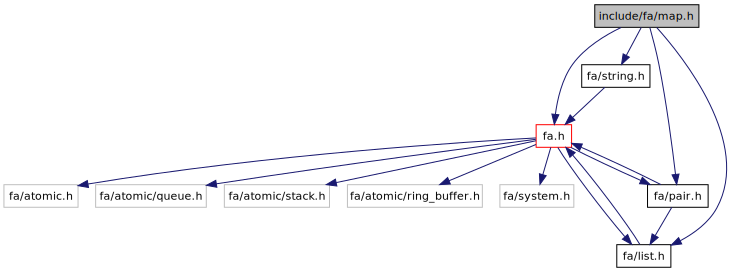
\includegraphics[width=350pt]{map_8h__incl}
\end{center}
\end{figure}
This graph shows which files directly or indirectly include this file\-:\nopagebreak
\begin{figure}[H]
\begin{center}
\leavevmode
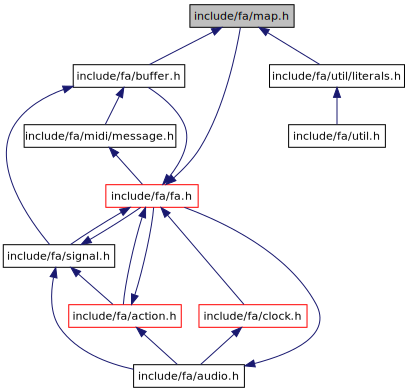
\includegraphics[width=350pt]{map_8h__dep__incl}
\end{center}
\end{figure}
\subsection*{Typedefs}
\begin{DoxyCompactItemize}
\item 
typedef struct \-\_\-fa\-\_\-map\-\_\-t $\ast$ \hyperlink{group___fa_map_gadcbb0c425af31be6aeb265159b2a7db0}{fa\-\_\-map\-\_\-t}
\item 
typedef \hyperlink{group___fa_ga915ddeae99ad7568b273d2b876425197}{fa\-\_\-ptr\-\_\-t} \hyperlink{group___fa_map_ga01c714699c14e805664c65b6a0ea974d}{fa\-\_\-map\-\_\-key\-\_\-t}
\end{DoxyCompactItemize}
\subsection*{Functions}
\begin{DoxyCompactItemize}
\item 
\hyperlink{group___fa_map_gadcbb0c425af31be6aeb265159b2a7db0}{fa\-\_\-map\-\_\-t} \hyperlink{group___fa_map_gab96a62b8c3900af432faa9c7fe9a06e6}{fa\-\_\-map\-\_\-empty} ()
\begin{DoxyCompactList}\small\item\em Create an empty list. \end{DoxyCompactList}\item 
\hyperlink{group___fa_map_gadcbb0c425af31be6aeb265159b2a7db0}{fa\-\_\-map\-\_\-t} \hyperlink{group___fa_map_ga6431b8636b6f9de2db5eabc130607ddf}{fa\-\_\-map\-\_\-copy} (\hyperlink{group___fa_map_gadcbb0c425af31be6aeb265159b2a7db0}{fa\-\_\-map\-\_\-t} \hyperlink{literals_8h_a44305f0bc81207be0dcc90650733e331}{map})
\begin{DoxyCompactList}\small\item\em Copy the given list. \end{DoxyCompactList}\item 
void \hyperlink{group___fa_map_gaecb6f294fd3614f34c7308ebd8a2e25a}{fa\-\_\-map\-\_\-destroy} (\hyperlink{group___fa_map_gadcbb0c425af31be6aeb265159b2a7db0}{fa\-\_\-map\-\_\-t} \hyperlink{literals_8h_a44305f0bc81207be0dcc90650733e331}{map})
\begin{DoxyCompactList}\small\item\em Destroy the given list. \end{DoxyCompactList}\item 
int \hyperlink{group___fa_map_ga2b48664b3fd7e1c080c4c5f8071427f0}{fa\-\_\-map\-\_\-size} (\hyperlink{group___fa_map_gadcbb0c425af31be6aeb265159b2a7db0}{fa\-\_\-map\-\_\-t} \hyperlink{literals_8h_a44305f0bc81207be0dcc90650733e331}{map})
\begin{DoxyCompactList}\small\item\em Return the number of elements in the given list. \end{DoxyCompactList}\item 
bool \hyperlink{group___fa_map_gae580cafd90c4447a7970096d5dff8f46}{fa\-\_\-map\-\_\-is\-\_\-empty} (\hyperlink{group___fa_map_gadcbb0c425af31be6aeb265159b2a7db0}{fa\-\_\-map\-\_\-t} \hyperlink{literals_8h_a44305f0bc81207be0dcc90650733e331}{map})
\begin{DoxyCompactList}\small\item\em Return whether the given list is empty. \end{DoxyCompactList}\item 
bool \hyperlink{group___fa_map_gaa3f04a11ae175c8b8f9f916d05293ed3}{fa\-\_\-map\-\_\-is\-\_\-single} (\hyperlink{group___fa_map_gadcbb0c425af31be6aeb265159b2a7db0}{fa\-\_\-map\-\_\-t} \hyperlink{literals_8h_a44305f0bc81207be0dcc90650733e331}{map})
\begin{DoxyCompactList}\small\item\em Return whether the given list has a single element. \end{DoxyCompactList}\item 
\hyperlink{group___fa_map_gadcbb0c425af31be6aeb265159b2a7db0}{fa\-\_\-map\-\_\-t} \hyperlink{group___fa_map_gaf8b3b5cdac0cd00691754f0c7a0f87c6}{fa\-\_\-map\-\_\-add} (\hyperlink{group___fa_map_ga01c714699c14e805664c65b6a0ea974d}{fa\-\_\-map\-\_\-key\-\_\-t} key, \hyperlink{group___fa_ga915ddeae99ad7568b273d2b876425197}{fa\-\_\-ptr\-\_\-t} ptr, \hyperlink{group___fa_map_gadcbb0c425af31be6aeb265159b2a7db0}{fa\-\_\-map\-\_\-t} \hyperlink{literals_8h_a44305f0bc81207be0dcc90650733e331}{map})
\begin{DoxyCompactList}\small\item\em Add an element to the map if not present. \end{DoxyCompactList}\item 
\hyperlink{group___fa_map_gadcbb0c425af31be6aeb265159b2a7db0}{fa\-\_\-map\-\_\-t} \hyperlink{group___fa_map_ga91b515cb8f096af2f6ab3f7588ae41aa}{fa\-\_\-map\-\_\-set} (\hyperlink{group___fa_map_ga01c714699c14e805664c65b6a0ea974d}{fa\-\_\-map\-\_\-key\-\_\-t} key, \hyperlink{group___fa_ga915ddeae99ad7568b273d2b876425197}{fa\-\_\-ptr\-\_\-t} ptr, \hyperlink{group___fa_map_gadcbb0c425af31be6aeb265159b2a7db0}{fa\-\_\-map\-\_\-t} \hyperlink{literals_8h_a44305f0bc81207be0dcc90650733e331}{map})
\begin{DoxyCompactList}\small\item\em Add an element to the map, replacing if already present. \end{DoxyCompactList}\item 
\hyperlink{group___fa_map_gadcbb0c425af31be6aeb265159b2a7db0}{fa\-\_\-map\-\_\-t} \hyperlink{group___fa_map_ga73d68f263f542b076d0ae0cf4a62b5dd}{fa\-\_\-map\-\_\-remove} (\hyperlink{group___fa_map_ga01c714699c14e805664c65b6a0ea974d}{fa\-\_\-map\-\_\-key\-\_\-t} key, \hyperlink{group___fa_map_gadcbb0c425af31be6aeb265159b2a7db0}{fa\-\_\-map\-\_\-t} \hyperlink{literals_8h_a44305f0bc81207be0dcc90650733e331}{map})
\begin{DoxyCompactList}\small\item\em Remove the given key if present. \end{DoxyCompactList}\item 
\hyperlink{group___fa_map_gadcbb0c425af31be6aeb265159b2a7db0}{fa\-\_\-map\-\_\-t} \hyperlink{group___fa_map_ga2597c509111f8e9d4231afda12a162bf}{fa\-\_\-map\-\_\-dadd} (\hyperlink{group___fa_map_ga01c714699c14e805664c65b6a0ea974d}{fa\-\_\-map\-\_\-key\-\_\-t} key, \hyperlink{group___fa_ga915ddeae99ad7568b273d2b876425197}{fa\-\_\-ptr\-\_\-t} ptr, \hyperlink{group___fa_map_gadcbb0c425af31be6aeb265159b2a7db0}{fa\-\_\-map\-\_\-t} \hyperlink{literals_8h_a44305f0bc81207be0dcc90650733e331}{map})
\begin{DoxyCompactList}\small\item\em Add an element to the map if not present. \end{DoxyCompactList}\item 
\hyperlink{group___fa_map_gadcbb0c425af31be6aeb265159b2a7db0}{fa\-\_\-map\-\_\-t} \hyperlink{group___fa_map_gab8babfab6a71dc62465932708705c604}{fa\-\_\-map\-\_\-dset} (\hyperlink{group___fa_map_ga01c714699c14e805664c65b6a0ea974d}{fa\-\_\-map\-\_\-key\-\_\-t} key, \hyperlink{group___fa_ga915ddeae99ad7568b273d2b876425197}{fa\-\_\-ptr\-\_\-t} ptr, \hyperlink{group___fa_map_gadcbb0c425af31be6aeb265159b2a7db0}{fa\-\_\-map\-\_\-t} \hyperlink{literals_8h_a44305f0bc81207be0dcc90650733e331}{map})
\begin{DoxyCompactList}\small\item\em Add an element to the map, replacing if already present. \end{DoxyCompactList}\item 
\hyperlink{group___fa_map_gadcbb0c425af31be6aeb265159b2a7db0}{fa\-\_\-map\-\_\-t} \hyperlink{group___fa_map_ga9dab19db8db2ae0912dca03bb326fd9f}{fa\-\_\-map\-\_\-dremove} (\hyperlink{group___fa_map_ga01c714699c14e805664c65b6a0ea974d}{fa\-\_\-map\-\_\-key\-\_\-t} key, \hyperlink{group___fa_map_gadcbb0c425af31be6aeb265159b2a7db0}{fa\-\_\-map\-\_\-t} \hyperlink{literals_8h_a44305f0bc81207be0dcc90650733e331}{map})
\begin{DoxyCompactList}\small\item\em Remove the given key if present. \end{DoxyCompactList}\item 
\hyperlink{group___fa_map_gadcbb0c425af31be6aeb265159b2a7db0}{fa\-\_\-map\-\_\-t} \hyperlink{group___fa_map_ga8b23fc1bb5a9803e477f8075ec9f04b6}{fa\-\_\-map\-\_\-add\-\_\-entry} (\hyperlink{group___fa_pair_gac2b2e58c230bac4f8a63ef6c05072680}{fa\-\_\-pair\-\_\-t} \hyperlink{util_8h_a40ed40659d2ed7f8712b0fe6ba6edebe}{pair}, \hyperlink{group___fa_map_gadcbb0c425af31be6aeb265159b2a7db0}{fa\-\_\-map\-\_\-t} \hyperlink{literals_8h_a44305f0bc81207be0dcc90650733e331}{map})
\begin{DoxyCompactList}\small\item\em Add an element to the map if not present. \end{DoxyCompactList}\item 
\hyperlink{group___fa_map_gadcbb0c425af31be6aeb265159b2a7db0}{fa\-\_\-map\-\_\-t} \hyperlink{group___fa_map_ga2f7b35137e12c3f63bf6c8492e438937}{fa\-\_\-map\-\_\-set\-\_\-entry} (\hyperlink{group___fa_pair_gac2b2e58c230bac4f8a63ef6c05072680}{fa\-\_\-pair\-\_\-t} \hyperlink{util_8h_a40ed40659d2ed7f8712b0fe6ba6edebe}{pair}, \hyperlink{group___fa_map_gadcbb0c425af31be6aeb265159b2a7db0}{fa\-\_\-map\-\_\-t} \hyperlink{literals_8h_a44305f0bc81207be0dcc90650733e331}{map})
\begin{DoxyCompactList}\small\item\em Add an element to the map, replacing if already present. \end{DoxyCompactList}\item 
\hyperlink{group___fa_map_gadcbb0c425af31be6aeb265159b2a7db0}{fa\-\_\-map\-\_\-t} \hyperlink{group___fa_map_ga3b4cb5d328675f599cbbf533cdec3860}{fa\-\_\-map\-\_\-remove\-\_\-entry} (\hyperlink{group___fa_pair_gac2b2e58c230bac4f8a63ef6c05072680}{fa\-\_\-pair\-\_\-t} \hyperlink{util_8h_a40ed40659d2ed7f8712b0fe6ba6edebe}{pair}, \hyperlink{group___fa_map_gadcbb0c425af31be6aeb265159b2a7db0}{fa\-\_\-map\-\_\-t} \hyperlink{literals_8h_a44305f0bc81207be0dcc90650733e331}{map})
\begin{DoxyCompactList}\small\item\em Remove the given key if present. \end{DoxyCompactList}\item 
\hyperlink{group___fa_ga915ddeae99ad7568b273d2b876425197}{fa\-\_\-ptr\-\_\-t} \hyperlink{group___fa_map_ga23e3bce2dfad5f3c7c2ef518dfe3ca70}{fa\-\_\-map\-\_\-get} (\hyperlink{group___fa_map_ga01c714699c14e805664c65b6a0ea974d}{fa\-\_\-map\-\_\-key\-\_\-t} key, \hyperlink{group___fa_map_gadcbb0c425af31be6aeb265159b2a7db0}{fa\-\_\-map\-\_\-t} \hyperlink{literals_8h_a44305f0bc81207be0dcc90650733e331}{map})
\begin{DoxyCompactList}\small\item\em Return the element stored at the given key, or {\ttfamily null} if the key does not exist. \end{DoxyCompactList}\item 
bool \hyperlink{group___fa_map_ga3bfe761e64c42dd57f7598a149b91808}{fa\-\_\-map\-\_\-has\-\_\-key} (\hyperlink{group___fa_map_ga01c714699c14e805664c65b6a0ea974d}{fa\-\_\-map\-\_\-key\-\_\-t} key, \hyperlink{group___fa_map_gadcbb0c425af31be6aeb265159b2a7db0}{fa\-\_\-map\-\_\-t} \hyperlink{literals_8h_a44305f0bc81207be0dcc90650733e331}{map})
\begin{DoxyCompactList}\small\item\em Return whether the given key exists in the given map. \end{DoxyCompactList}\item 
bool \hyperlink{group___fa_map_gac36e905827b6b35ce95fb8add39ec61a}{fa\-\_\-map\-\_\-has\-\_\-elem} (\hyperlink{group___fa_ga915ddeae99ad7568b273d2b876425197}{fa\-\_\-ptr\-\_\-t} ptr, \hyperlink{group___fa_map_gadcbb0c425af31be6aeb265159b2a7db0}{fa\-\_\-map\-\_\-t} \hyperlink{literals_8h_a44305f0bc81207be0dcc90650733e331}{map})
\begin{DoxyCompactList}\small\item\em Return whether the given element exists in the given map. \end{DoxyCompactList}\item 
bool \hyperlink{group___fa_map_ga7001e19d64d3e0a95c4f49ec07c06ea9}{fa\-\_\-map\-\_\-has\-\_\-entry} (\hyperlink{group___fa_pair_gac2b2e58c230bac4f8a63ef6c05072680}{fa\-\_\-pair\-\_\-t} \hyperlink{util_8h_a40ed40659d2ed7f8712b0fe6ba6edebe}{pair}, \hyperlink{group___fa_map_gadcbb0c425af31be6aeb265159b2a7db0}{fa\-\_\-map\-\_\-t} \hyperlink{literals_8h_a44305f0bc81207be0dcc90650733e331}{map})
\begin{DoxyCompactList}\small\item\em Return whether the given \$(key, element)\$ pair element exists in the given map. \end{DoxyCompactList}\item 
bool \hyperlink{group___fa_map_ga589cc956fd74abb3fcd05fbc96ae1874}{fa\-\_\-map\-\_\-is\-\_\-submap\-\_\-of} (\hyperlink{group___fa_map_gadcbb0c425af31be6aeb265159b2a7db0}{fa\-\_\-map\-\_\-t} \hyperlink{literals_8h_a44305f0bc81207be0dcc90650733e331}{map}, \hyperlink{group___fa_map_gadcbb0c425af31be6aeb265159b2a7db0}{fa\-\_\-map\-\_\-t} map\-\_\-)
\begin{DoxyCompactList}\small\item\em Whether the first of the given maps is a submap of the second. \end{DoxyCompactList}\item 
bool \hyperlink{group___fa_map_ga9a003ebb1dd563e308197eede6bfd3c2}{fa\-\_\-map\-\_\-is\-\_\-proper\-\_\-submap\-\_\-of} (\hyperlink{group___fa_map_gadcbb0c425af31be6aeb265159b2a7db0}{fa\-\_\-map\-\_\-t} \hyperlink{literals_8h_a44305f0bc81207be0dcc90650733e331}{map}, \hyperlink{group___fa_map_gadcbb0c425af31be6aeb265159b2a7db0}{fa\-\_\-map\-\_\-t} map\-\_\-)
\begin{DoxyCompactList}\small\item\em Whether the first of the given maps is a proper submap of the second. \end{DoxyCompactList}\item 
\hyperlink{group___fa_map_gadcbb0c425af31be6aeb265159b2a7db0}{fa\-\_\-map\-\_\-t} \hyperlink{group___fa_map_gaf80408d1f455d54c3fd3d6a85e63850d}{fa\-\_\-map\-\_\-sum} (\hyperlink{group___fa_map_gadcbb0c425af31be6aeb265159b2a7db0}{fa\-\_\-map\-\_\-t} \hyperlink{literals_8h_a44305f0bc81207be0dcc90650733e331}{map}, \hyperlink{group___fa_map_gadcbb0c425af31be6aeb265159b2a7db0}{fa\-\_\-map\-\_\-t} map\-\_\-)
\begin{DoxyCompactList}\small\item\em Sum or union of the given maps. \end{DoxyCompactList}\item 
\hyperlink{group___fa_map_gadcbb0c425af31be6aeb265159b2a7db0}{fa\-\_\-map\-\_\-t} \hyperlink{group___fa_map_ga334ae2424a14e058580286645ee0aaf4}{fa\-\_\-map\-\_\-product} (\hyperlink{group___fa_map_gadcbb0c425af31be6aeb265159b2a7db0}{fa\-\_\-map\-\_\-t} \hyperlink{literals_8h_a44305f0bc81207be0dcc90650733e331}{map}, \hyperlink{group___fa_map_gadcbb0c425af31be6aeb265159b2a7db0}{fa\-\_\-map\-\_\-t} map\-\_\-)
\begin{DoxyCompactList}\small\item\em Cartesian product of the given maps. \end{DoxyCompactList}\item 
\hyperlink{group___fa_map_gadcbb0c425af31be6aeb265159b2a7db0}{fa\-\_\-map\-\_\-t} \hyperlink{group___fa_map_gaa957b7099132ca05f5cd719699d3117c}{fa\-\_\-map\-\_\-difference} (\hyperlink{group___fa_map_gadcbb0c425af31be6aeb265159b2a7db0}{fa\-\_\-map\-\_\-t} \hyperlink{literals_8h_a44305f0bc81207be0dcc90650733e331}{map}, \hyperlink{group___fa_map_gadcbb0c425af31be6aeb265159b2a7db0}{fa\-\_\-map\-\_\-t} map\-\_\-)
\begin{DoxyCompactList}\small\item\em Symmetric difference of the given maps. \end{DoxyCompactList}\item 
\hyperlink{group___fa_map_gadcbb0c425af31be6aeb265159b2a7db0}{fa\-\_\-map\-\_\-t} \hyperlink{group___fa_map_gaa2ddc5a471acd60dccd6b130d7bad863}{fa\-\_\-map\-\_\-map} (\hyperlink{group___fa_gaaafae8ab9ebae9019133108e56d2d4d1}{fa\-\_\-unary\-\_\-t} unary, \hyperlink{group___fa_ga915ddeae99ad7568b273d2b876425197}{fa\-\_\-ptr\-\_\-t} ptr, \hyperlink{group___fa_map_gadcbb0c425af31be6aeb265159b2a7db0}{fa\-\_\-map\-\_\-t} \hyperlink{literals_8h_a44305f0bc81207be0dcc90650733e331}{map})
\begin{DoxyCompactList}\small\item\em Return the result of applying the given function to all elements of the given list. \end{DoxyCompactList}\item 
\hyperlink{group___fa_map_gadcbb0c425af31be6aeb265159b2a7db0}{fa\-\_\-map\-\_\-t} \hyperlink{group___fa_map_ga8a1decfa57fb6d688155de6edc9d8dba}{fa\-\_\-map\-\_\-from\-\_\-pair} (\hyperlink{group___fa_pair_gac2b2e58c230bac4f8a63ef6c05072680}{fa\-\_\-pair\-\_\-t} \hyperlink{util_8h_a40ed40659d2ed7f8712b0fe6ba6edebe}{pair})
\begin{DoxyCompactList}\small\item\em Convert the given pair to a map. \end{DoxyCompactList}\item 
\hyperlink{group___fa_map_gadcbb0c425af31be6aeb265159b2a7db0}{fa\-\_\-map\-\_\-t} \hyperlink{group___fa_map_gacfe8c751a747fee0ef908c4d5e6de1d0}{fa\-\_\-map\-\_\-from\-\_\-list} (\hyperlink{group___fa_list_ga35ecb12ab934ded0cce0bcf28e3bc5d2}{fa\-\_\-list\-\_\-t} \hyperlink{literals_8h_a4ddd63dfcfec2b4d5741a56aa6003c76}{list})
\begin{DoxyCompactList}\small\item\em Convert the given list to a map. \end{DoxyCompactList}\item 
\hyperlink{group___fa_list_ga35ecb12ab934ded0cce0bcf28e3bc5d2}{fa\-\_\-list\-\_\-t} \hyperlink{group___fa_map_ga37672df6747bddc854e8b3d162958335}{fa\-\_\-map\-\_\-to\-\_\-list} (\hyperlink{group___fa_map_gadcbb0c425af31be6aeb265159b2a7db0}{fa\-\_\-map\-\_\-t} \hyperlink{literals_8h_a44305f0bc81207be0dcc90650733e331}{map})
\begin{DoxyCompactList}\small\item\em Convert the given map to a list. \end{DoxyCompactList}\end{DoxyCompactItemize}

\hypertarget{midi_8h}{\section{include/fa/midi.h File Reference}
\label{midi_8h}\index{include/fa/midi.\-h@{include/fa/midi.\-h}}
}
{\ttfamily \#include $<$fa/list.\-h$>$}\\*
{\ttfamily \#include $<$fa/pair.\-h$>$}\\*
{\ttfamily \#include $<$fa/action.\-h$>$}\\*
{\ttfamily \#include $<$fa/time.\-h$>$}\\*
{\ttfamily \#include $<$fa/clock.\-h$>$}\\*
{\ttfamily \#include $<$fa/error.\-h$>$}\\*
Include dependency graph for midi.\-h\-:\nopagebreak
\begin{figure}[H]
\begin{center}
\leavevmode
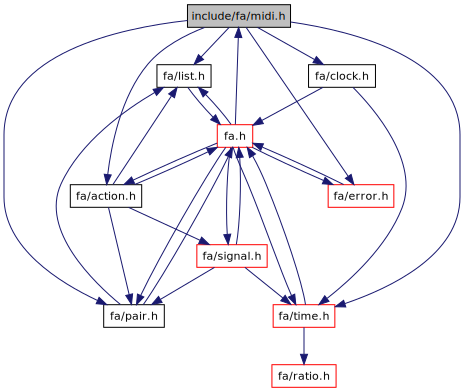
\includegraphics[width=350pt]{midi_8h__incl}
\end{center}
\end{figure}
This graph shows which files directly or indirectly include this file\-:\nopagebreak
\begin{figure}[H]
\begin{center}
\leavevmode
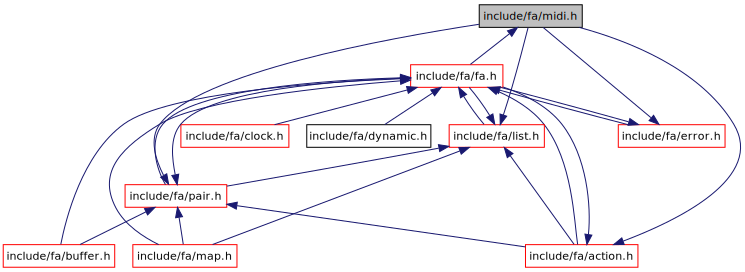
\includegraphics[width=350pt]{midi_8h__dep__incl}
\end{center}
\end{figure}
\subsection*{Typedefs}
\begin{DoxyCompactItemize}
\item 
typedef struct \-\_\-fa\-\_\-midi\-\_\-device\-\_\-t $\ast$ \hyperlink{group___fa_midi_gabbbfd1ec30a186768ba2744e46bacc9b}{fa\-\_\-midi\-\_\-device\-\_\-t}
\begin{DoxyCompactList}\small\item\em A M\-I\-D\-I device. \end{DoxyCompactList}\item 
typedef struct \-\_\-fa\-\_\-midi\-\_\-session\-\_\-t $\ast$ \hyperlink{group___fa_midi_ga222964548b932c6f53b575b23629530e}{fa\-\_\-midi\-\_\-session\-\_\-t}
\begin{DoxyCompactList}\small\item\em A M\-I\-D\-I session. \end{DoxyCompactList}\item 
typedef struct \-\_\-fa\-\_\-midi\-\_\-stream\-\_\-t $\ast$ \hyperlink{group___fa_midi_ga85772039b62d8bb718a51e1ffbbb2fa2}{fa\-\_\-midi\-\_\-stream\-\_\-t}
\begin{DoxyCompactList}\small\item\em A M\-I\-D\-I stream. \end{DoxyCompactList}\item 
typedef \hyperlink{group___fa_midi_ga222964548b932c6f53b575b23629530e}{fa\-\_\-midi\-\_\-session\-\_\-t}($\ast$ \hyperlink{group___fa_midi_ga20fb39192d8af433b1506a529bc981e7}{fa\-\_\-midi\-\_\-session\-\_\-callback\-\_\-t} )(\hyperlink{group___fa_ga915ddeae99ad7568b273d2b876425197}{fa\-\_\-ptr\-\_\-t}, \hyperlink{group___fa_midi_ga222964548b932c6f53b575b23629530e}{fa\-\_\-midi\-\_\-session\-\_\-t})
\begin{DoxyCompactList}\small\item\em A callback to receive M\-I\-D\-I sessions. \end{DoxyCompactList}\item 
typedef \hyperlink{group___fa_midi_ga85772039b62d8bb718a51e1ffbbb2fa2}{fa\-\_\-midi\-\_\-stream\-\_\-t}($\ast$ \hyperlink{group___fa_midi_ga8022098ffcf993ccdaed068b97ab7bfc}{fa\-\_\-midi\-\_\-stream\-\_\-callback\-\_\-t} )(\hyperlink{group___fa_ga915ddeae99ad7568b273d2b876425197}{fa\-\_\-ptr\-\_\-t}, \hyperlink{group___fa_midi_ga85772039b62d8bb718a51e1ffbbb2fa2}{fa\-\_\-midi\-\_\-stream\-\_\-t})
\begin{DoxyCompactList}\small\item\em A callback to receive M\-I\-D\-I streams. \end{DoxyCompactList}\item 
typedef \hyperlink{group___fa_ga43b940a9294fd58a54087ef0b416e479}{fa\-\_\-nullary\-\_\-t} \hyperlink{group___fa_midi_gacc769aa23b097e8b8dc3d4807b9a066d}{fa\-\_\-midi\-\_\-status\-\_\-callback\-\_\-t}
\begin{DoxyCompactList}\small\item\em A callback to be invoked upon changes to the M\-I\-D\-I setup. \end{DoxyCompactList}\item 
typedef \hyperlink{group___fa_gaaafae8ab9ebae9019133108e56d2d4d1}{fa\-\_\-unary\-\_\-t} \hyperlink{group___fa_midi_ga446c3043288f44554ba1c69ab03f4a1d}{fa\-\_\-midi\-\_\-message\-\_\-callback\-\_\-t}
\begin{DoxyCompactList}\small\item\em A callback to be invoked whenever a message is received. \end{DoxyCompactList}\end{DoxyCompactItemize}
\subsection*{Functions}
\begin{DoxyCompactItemize}
\item 
\hyperlink{group___fa_midi_ga222964548b932c6f53b575b23629530e}{fa\-\_\-midi\-\_\-session\-\_\-t} \hyperlink{group___fa_midi_ga2f1b526042c4356ce7e2adcf0d11ecad}{fa\-\_\-midi\-\_\-begin\-\_\-session} ()
\begin{DoxyCompactList}\small\item\em Begin a new midi session. \end{DoxyCompactList}\item 
void \hyperlink{group___fa_midi_gaa17624fa01a142329eef651bf58867ec}{fa\-\_\-midi\-\_\-end\-\_\-session} (\hyperlink{group___fa_midi_ga222964548b932c6f53b575b23629530e}{fa\-\_\-midi\-\_\-session\-\_\-t} session)
\begin{DoxyCompactList}\small\item\em End the given session. \end{DoxyCompactList}\item 
void \hyperlink{group___fa_midi_gaae4f24a325199a994a64d9d13023164d}{fa\-\_\-midi\-\_\-with\-\_\-session} (\hyperlink{group___fa_midi_ga20fb39192d8af433b1506a529bc981e7}{fa\-\_\-midi\-\_\-session\-\_\-callback\-\_\-t} session\-Callback, \hyperlink{group___fa_ga915ddeae99ad7568b273d2b876425197}{fa\-\_\-ptr\-\_\-t} ptr, \hyperlink{group___fa_error_ga43d8d45a005130a5052ba3281a8bf33e}{fa\-\_\-error\-\_\-callback\-\_\-t} callback, \hyperlink{group___fa_ga915ddeae99ad7568b273d2b876425197}{fa\-\_\-ptr\-\_\-t} ptr\-\_\-)
\begin{DoxyCompactList}\small\item\em Begin a new session, and retain it for the duration of a call to the given function. \end{DoxyCompactList}\item 
\hyperlink{group___fa_list_ga35ecb12ab934ded0cce0bcf28e3bc5d2}{fa\-\_\-list\-\_\-t} \hyperlink{group___fa_midi_gaf7d4af506bd8ec5194a2952346b968d7}{fa\-\_\-midi\-\_\-current\-\_\-sessions} ()
\begin{DoxyCompactList}\small\item\em Get all currently active M\-I\-D\-I sessions. \end{DoxyCompactList}\item 
\hyperlink{group___fa_ga915ddeae99ad7568b273d2b876425197}{fa\-\_\-ptr\-\_\-t} \hyperlink{group___fa_midi_ga7bd603a4286ddff81c1fd7c7656b4255}{fa\-\_\-midi\-\_\-end\-\_\-all\-\_\-sessions} ()
\begin{DoxyCompactList}\small\item\em End all currently active M\-I\-D\-I sessions. \end{DoxyCompactList}\item 
\hyperlink{group___fa_list_ga35ecb12ab934ded0cce0bcf28e3bc5d2}{fa\-\_\-list\-\_\-t} \hyperlink{group___fa_midi_gafbb8556093f979db2a0b3483e40c6da3}{fa\-\_\-midi\-\_\-all} (\hyperlink{group___fa_midi_ga222964548b932c6f53b575b23629530e}{fa\-\_\-midi\-\_\-session\-\_\-t} session)
\begin{DoxyCompactList}\small\item\em Get all active midi devices of the given session. \end{DoxyCompactList}\item 
\hyperlink{group___fa_pair_gac2b2e58c230bac4f8a63ef6c05072680}{fa\-\_\-pair\-\_\-t} \hyperlink{group___fa_midi_gab20056f966f2be60bd4be8279b74c893}{fa\-\_\-midi\-\_\-default} (\hyperlink{group___fa_midi_ga222964548b932c6f53b575b23629530e}{fa\-\_\-midi\-\_\-session\-\_\-t} session)
\begin{DoxyCompactList}\small\item\em Get the standard devices of the given session. \end{DoxyCompactList}\item 
\hyperlink{group___fa_midi_gabbbfd1ec30a186768ba2744e46bacc9b}{fa\-\_\-midi\-\_\-device\-\_\-t} \hyperlink{group___fa_midi_ga4e47ae817979dbce0da298466e97da75}{fa\-\_\-midi\-\_\-default\-\_\-input} (\hyperlink{group___fa_midi_ga222964548b932c6f53b575b23629530e}{fa\-\_\-midi\-\_\-session\-\_\-t} session)
\begin{DoxyCompactList}\small\item\em Get the standard input device of the given session. \end{DoxyCompactList}\item 
\hyperlink{group___fa_midi_gabbbfd1ec30a186768ba2744e46bacc9b}{fa\-\_\-midi\-\_\-device\-\_\-t} \hyperlink{group___fa_midi_gad859725831a5227e58a53e867af798b3}{fa\-\_\-midi\-\_\-default\-\_\-output} (\hyperlink{group___fa_midi_ga222964548b932c6f53b575b23629530e}{fa\-\_\-midi\-\_\-session\-\_\-t} session)
\begin{DoxyCompactList}\small\item\em Get the standard output device of the given session. \end{DoxyCompactList}\item 
void \hyperlink{group___fa_midi_ga448ae46b23a1271b7be8fb44ae88dbc9}{fa\-\_\-midi\-\_\-add\-\_\-status\-\_\-callback} (\hyperlink{group___fa_midi_gacc769aa23b097e8b8dc3d4807b9a066d}{fa\-\_\-midi\-\_\-status\-\_\-callback\-\_\-t} status\-Callback, \hyperlink{group___fa_ga915ddeae99ad7568b273d2b876425197}{fa\-\_\-ptr\-\_\-t} ptr, \hyperlink{group___fa_midi_ga222964548b932c6f53b575b23629530e}{fa\-\_\-midi\-\_\-session\-\_\-t} session)
\begin{DoxyCompactList}\small\item\em Register a callback to be invoked when a hardware change is detected. \end{DoxyCompactList}\item 
\hyperlink{group___fa_string_gacada63033b77bc6c39fa632ae199349b}{fa\-\_\-string\-\_\-t} \hyperlink{group___fa_midi_ga4ed5065817addf704612c41e2e6ec753}{fa\-\_\-midi\-\_\-name} (\hyperlink{group___fa_midi_gabbbfd1ec30a186768ba2744e46bacc9b}{fa\-\_\-midi\-\_\-device\-\_\-t} device)
\begin{DoxyCompactList}\small\item\em Return the name of the given device. \end{DoxyCompactList}\item 
\hyperlink{group___fa_string_gacada63033b77bc6c39fa632ae199349b}{fa\-\_\-string\-\_\-t} \hyperlink{group___fa_midi_ga370b7d98e395878426f1c91104e40489}{fa\-\_\-midi\-\_\-host\-\_\-name} (\hyperlink{group___fa_midi_gabbbfd1ec30a186768ba2744e46bacc9b}{fa\-\_\-midi\-\_\-device\-\_\-t} device)
\begin{DoxyCompactList}\small\item\em Return the host name of the given device. \end{DoxyCompactList}\item 
bool \hyperlink{group___fa_midi_ga50b48cf8b0f607418a9c9720b3f1f50e}{fa\-\_\-midi\-\_\-has\-\_\-input} (\hyperlink{group___fa_midi_gabbbfd1ec30a186768ba2744e46bacc9b}{fa\-\_\-midi\-\_\-device\-\_\-t} device)
\begin{DoxyCompactList}\small\item\em Return whether the given device has input or not. \end{DoxyCompactList}\item 
bool \hyperlink{group___fa_midi_gaa86f40de5a25870a92e962e45dcb43a6}{fa\-\_\-midi\-\_\-has\-\_\-output} (\hyperlink{group___fa_midi_gabbbfd1ec30a186768ba2744e46bacc9b}{fa\-\_\-midi\-\_\-device\-\_\-t} device)
\begin{DoxyCompactList}\small\item\em Return whether the given device has output or not. \end{DoxyCompactList}\item 
\hyperlink{group___fa_midi_ga85772039b62d8bb718a51e1ffbbb2fa2}{fa\-\_\-midi\-\_\-stream\-\_\-t} \hyperlink{group___fa_midi_gab7b05f67b7966c706652a292bb9e7a65}{fa\-\_\-midi\-\_\-open\-\_\-stream} (\hyperlink{group___fa_midi_gabbbfd1ec30a186768ba2744e46bacc9b}{fa\-\_\-midi\-\_\-device\-\_\-t} device)
\begin{DoxyCompactList}\small\item\em Open a stream on the given devices. \end{DoxyCompactList}\item 
void \hyperlink{group___fa_midi_ga8a306a27cb08528a31b9fdad6b4f75ab}{fa\-\_\-midi\-\_\-close\-\_\-stream} (\hyperlink{group___fa_midi_ga85772039b62d8bb718a51e1ffbbb2fa2}{fa\-\_\-midi\-\_\-stream\-\_\-t} stream)
\begin{DoxyCompactList}\small\item\em Close the given stream. \end{DoxyCompactList}\item 
void \hyperlink{group___fa_midi_ga2b3813b25c03a1c609afd039e7565599}{fa\-\_\-midi\-\_\-with\-\_\-stream} (\hyperlink{group___fa_midi_gabbbfd1ec30a186768ba2744e46bacc9b}{fa\-\_\-midi\-\_\-device\-\_\-t} device, \hyperlink{group___fa_midi_ga8022098ffcf993ccdaed068b97ab7bfc}{fa\-\_\-midi\-\_\-stream\-\_\-callback\-\_\-t} stream\-Callback, \hyperlink{group___fa_ga915ddeae99ad7568b273d2b876425197}{fa\-\_\-ptr\-\_\-t} ptr, \hyperlink{group___fa_error_ga43d8d45a005130a5052ba3281a8bf33e}{fa\-\_\-error\-\_\-callback\-\_\-t} callback, \hyperlink{group___fa_ga915ddeae99ad7568b273d2b876425197}{fa\-\_\-ptr\-\_\-t} ptr\-\_\-)
\begin{DoxyCompactList}\small\item\em Run a stream on the given devices. \end{DoxyCompactList}\item 
void \hyperlink{group___fa_midi_ga52859a899712bbbac285d7474f546bf0}{fa\-\_\-midi\-\_\-add\-\_\-message\-\_\-callback} (\hyperlink{group___fa_midi_ga446c3043288f44554ba1c69ab03f4a1d}{fa\-\_\-midi\-\_\-message\-\_\-callback\-\_\-t} message\-Callback, \hyperlink{group___fa_ga915ddeae99ad7568b273d2b876425197}{fa\-\_\-ptr\-\_\-t} ptr, \hyperlink{group___fa_midi_ga85772039b62d8bb718a51e1ffbbb2fa2}{fa\-\_\-midi\-\_\-stream\-\_\-t} stream)
\begin{DoxyCompactList}\small\item\em Register a callback to be invoked when a message is received. \end{DoxyCompactList}\item 
void \hyperlink{group___fa_midi_gacfa36ef71f8c8d797a040e35b72aff58}{fa\-\_\-midi\-\_\-set\-\_\-clock} (\hyperlink{group___fa_midi_ga85772039b62d8bb718a51e1ffbbb2fa2}{fa\-\_\-midi\-\_\-stream\-\_\-t} stream, \hyperlink{group___fa_clock_ga20b3a0f49788fbedba140b1d315d2313}{fa\-\_\-clock\-\_\-t} clock)
\begin{DoxyCompactList}\small\item\em Associate the given clock with the given stream. \end{DoxyCompactList}\item 
\hyperlink{group___fa_clock_ga20b3a0f49788fbedba140b1d315d2313}{fa\-\_\-clock\-\_\-t} \hyperlink{group___fa_midi_ga120b0e56a83ab18da64499570e22c7b7}{fa\-\_\-midi\-\_\-get\-\_\-clock} (\hyperlink{group___fa_midi_ga85772039b62d8bb718a51e1ffbbb2fa2}{fa\-\_\-midi\-\_\-stream\-\_\-t} stream)
\begin{DoxyCompactList}\small\item\em Return the clock associated with a given stream. \end{DoxyCompactList}\item 
void \hyperlink{group___fa_midi_ga9a269b2817ba3371d5b58493e33c0229}{fa\-\_\-midi\-\_\-schedule} (\hyperlink{group___fa_time_ga227cc693f20b4873fed11028bcade184}{fa\-\_\-time\-\_\-t} time, \hyperlink{group___fa_action_gadb08ae063168671e5fedc6c23f20ae4b}{fa\-\_\-action\-\_\-t} action, \hyperlink{group___fa_midi_ga85772039b62d8bb718a51e1ffbbb2fa2}{fa\-\_\-midi\-\_\-stream\-\_\-t} stream)
\begin{DoxyCompactList}\small\item\em Schedule an action on the stream. \end{DoxyCompactList}\item 
void \hyperlink{group___fa_midi_ga69d4b4f30d7cb997df0ff26b61f94400}{fa\-\_\-midi\-\_\-schedule\-\_\-relative} (\hyperlink{group___fa_time_ga227cc693f20b4873fed11028bcade184}{fa\-\_\-time\-\_\-t} time, \hyperlink{group___fa_action_gadb08ae063168671e5fedc6c23f20ae4b}{fa\-\_\-action\-\_\-t} action, \hyperlink{group___fa_midi_ga85772039b62d8bb718a51e1ffbbb2fa2}{fa\-\_\-midi\-\_\-stream\-\_\-t} stream)
\begin{DoxyCompactList}\small\item\em Schedule an action on the stream. \end{DoxyCompactList}\end{DoxyCompactItemize}

\hypertarget{message_8h}{\section{include/fa/midi/message.h File Reference}
\label{message_8h}\index{include/fa/midi/message.\-h@{include/fa/midi/message.\-h}}
}
{\ttfamily \#include $<$fa/std.\-h$>$}\\*
{\ttfamily \#include $<$fa/pair.\-h$>$}\\*
{\ttfamily \#include $<$fa/buffer.\-h$>$}\\*
Include dependency graph for message.\-h\-:\nopagebreak
\begin{figure}[H]
\begin{center}
\leavevmode
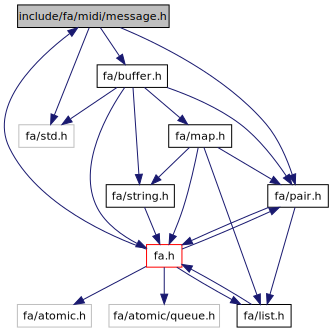
\includegraphics[width=350pt]{message_8h__incl}
\end{center}
\end{figure}
This graph shows which files directly or indirectly include this file\-:\nopagebreak
\begin{figure}[H]
\begin{center}
\leavevmode
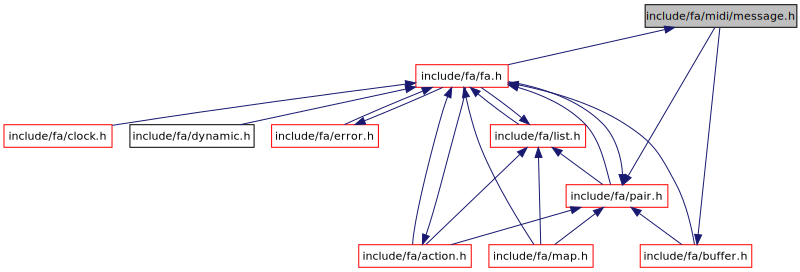
\includegraphics[width=350pt]{message_8h__dep__incl}
\end{center}
\end{figure}
\subsection*{Typedefs}
\begin{DoxyCompactItemize}
\item 
typedef int \hyperlink{group___fa_midi_message_gae7fc48e105b9bec5500bc422231a1159}{fa\-\_\-midi\-\_\-message\-\_\-channel\-\_\-t}
\item 
typedef int \hyperlink{group___fa_midi_message_gadc3c487a2892db5309395922f92e8d28}{fa\-\_\-midi\-\_\-message\-\_\-data\-\_\-t}
\item 
typedef struct \-\_\-fa\-\_\-midi\-\_\-message\-\_\-t $\ast$ \hyperlink{group___fa_midi_message_gaa73293eb40a2cffdc2294e3cb6dc2564}{fa\-\_\-midi\-\_\-message\-\_\-t}
\end{DoxyCompactItemize}
\subsection*{Enumerations}
\begin{DoxyCompactItemize}
\item 
enum \hyperlink{group___fa_midi_message_gaf34878eefb2ec676b7894176528d5b05}{fa\-\_\-midi\-\_\-message\-\_\-status\-\_\-t} \{ \\*
\hyperlink{group___fa_midi_message_ggaf34878eefb2ec676b7894176528d5b05aca154ab360fdd6f9578d9a301d634bcb}{note\-\_\-off}, 
\hyperlink{group___fa_midi_message_ggaf34878eefb2ec676b7894176528d5b05aa3aad707828be70a9dad4f256c1a0a28}{note\-\_\-on}, 
\hyperlink{group___fa_midi_message_ggaf34878eefb2ec676b7894176528d5b05a6586f26d582b52e7f4c3bd4fd32bf814}{after\-\_\-touch}, 
\hyperlink{group___fa_midi_message_ggaf34878eefb2ec676b7894176528d5b05ab6bf71590067f051c8e0c3c7e114442c}{control\-\_\-change}, 
\\*
\hyperlink{group___fa_midi_message_ggaf34878eefb2ec676b7894176528d5b05ab4d364a14ba45bcc49464e6e5e4cc60e}{program\-\_\-change}, 
\hyperlink{group___fa_midi_message_ggaf34878eefb2ec676b7894176528d5b05ae5e28da496463f48ff30c639c8a54950}{channel\-\_\-pressure}, 
\hyperlink{group___fa_midi_message_ggaf34878eefb2ec676b7894176528d5b05ac5197e881e3d9989c62d322e63c0affe}{pitch\-\_\-wheel}, 
\hyperlink{group___fa_midi_message_ggaf34878eefb2ec676b7894176528d5b05a2868e44729ef465f8774fb5bd3947fca}{sysex}
 \}
\end{DoxyCompactItemize}
\subsection*{Functions}
\begin{DoxyCompactItemize}
\item 
\hyperlink{group___fa_midi_message_gaa73293eb40a2cffdc2294e3cb6dc2564}{fa\-\_\-midi\-\_\-message\-\_\-t} \hyperlink{group___fa_midi_message_ga8f2f770703788aabdf9100161560d0de}{fa\-\_\-midi\-\_\-message\-\_\-create\-\_\-simple} (\hyperlink{group___fa_midi_message_gaf34878eefb2ec676b7894176528d5b05}{fa\-\_\-midi\-\_\-message\-\_\-status\-\_\-t} status, int int\-\_\-, int int\-\_\-\-\_\-)
\begin{DoxyCompactList}\small\item\em Creates a simple message from the given components. \end{DoxyCompactList}\item 
\hyperlink{group___fa_midi_message_gaa73293eb40a2cffdc2294e3cb6dc2564}{fa\-\_\-midi\-\_\-message\-\_\-t} \hyperlink{group___fa_midi_message_ga54d41c4ec0d77e9683ed1722cd4a9deb}{fa\-\_\-midi\-\_\-message\-\_\-create\-\_\-sysex} (\hyperlink{group___fa_buffer_ga0ed7a1d783ab322e2e8be02432d0839e}{fa\-\_\-buffer\-\_\-t} \hyperlink{util_8h_ad0c623e8b04565926f5b48888327724a}{buffer})
\begin{DoxyCompactList}\small\item\em Creates a sysex message from the given data buffer (not including F0 and F7). \end{DoxyCompactList}\item 
\hyperlink{group___fa_midi_message_gaa73293eb40a2cffdc2294e3cb6dc2564}{fa\-\_\-midi\-\_\-message\-\_\-t} \hyperlink{group___fa_midi_message_ga3054f30aab3248d85dcfa449a40a74ad}{fa\-\_\-midi\-\_\-message\-\_\-copy} (\hyperlink{group___fa_midi_message_gaa73293eb40a2cffdc2294e3cb6dc2564}{fa\-\_\-midi\-\_\-message\-\_\-t} message)
\begin{DoxyCompactList}\small\item\em Copy the given midi message. \end{DoxyCompactList}\item 
void \hyperlink{group___fa_midi_message_gaf8efe0ff27b3877bbdc47f6c1c0c95ec}{fa\-\_\-midi\-\_\-message\-\_\-destroy} (\hyperlink{group___fa_midi_message_gaa73293eb40a2cffdc2294e3cb6dc2564}{fa\-\_\-midi\-\_\-message\-\_\-t} message)
\begin{DoxyCompactList}\small\item\em Destroy the given midi\-\_\-message message. \end{DoxyCompactList}\item 
bool \hyperlink{group___fa_midi_message_ga21acffcd72a6a1ca793927d7533623fc}{fa\-\_\-midi\-\_\-message\-\_\-is\-\_\-simple} (\hyperlink{group___fa_midi_message_gaa73293eb40a2cffdc2294e3cb6dc2564}{fa\-\_\-midi\-\_\-message\-\_\-t} message)
\begin{DoxyCompactList}\small\item\em Return whether the given midi\-\_\-message message is a simple message. \end{DoxyCompactList}\item 
\hyperlink{group___fa_pair_gac2b2e58c230bac4f8a63ef6c05072680}{fa\-\_\-pair\-\_\-t} \hyperlink{group___fa_midi_message_gabc4f2eca0eba71269aadf05a9af534b1}{fa\-\_\-midi\-\_\-message\-\_\-simple\-\_\-data} (\hyperlink{group___fa_midi_message_gaa73293eb40a2cffdc2294e3cb6dc2564}{fa\-\_\-midi\-\_\-message\-\_\-t} message)
\begin{DoxyCompactList}\small\item\em Returns the status and channel part of a M\-I\-D\-I message. \end{DoxyCompactList}\item 
\hyperlink{group___fa_midi_message_gaf34878eefb2ec676b7894176528d5b05}{fa\-\_\-midi\-\_\-message\-\_\-status\-\_\-t} \hyperlink{group___fa_midi_message_gae7ca84ade26ff713f30555c2dd7dfc45}{fa\-\_\-midi\-\_\-message\-\_\-status} (\hyperlink{group___fa_midi_message_gaa73293eb40a2cffdc2294e3cb6dc2564}{fa\-\_\-midi\-\_\-message\-\_\-t} message)
\begin{DoxyCompactList}\small\item\em Return the status byte of given M\-I\-D\-I message. \end{DoxyCompactList}\item 
\hyperlink{group___fa_midi_message_gae7fc48e105b9bec5500bc422231a1159}{fa\-\_\-midi\-\_\-message\-\_\-channel\-\_\-t} \hyperlink{group___fa_midi_message_gab9d0873ebfcb0b112e1fb63db84d389c}{fa\-\_\-midi\-\_\-message\-\_\-channel} (\hyperlink{group___fa_midi_message_gaa73293eb40a2cffdc2294e3cb6dc2564}{fa\-\_\-midi\-\_\-message\-\_\-t} message)
\begin{DoxyCompactList}\small\item\em Return the channel byte of given M\-I\-D\-I message. \end{DoxyCompactList}\item 
bool \hyperlink{group___fa_midi_message_ga623772138041edb8566be99ebbae91f3}{fa\-\_\-midi\-\_\-message\-\_\-is\-\_\-sysex} (\hyperlink{group___fa_midi_message_gaa73293eb40a2cffdc2294e3cb6dc2564}{fa\-\_\-midi\-\_\-message\-\_\-t} message)
\begin{DoxyCompactList}\small\item\em Return whether the given M\-I\-D\-I message is a sysex message. \end{DoxyCompactList}\item 
\hyperlink{group___fa_buffer_ga0ed7a1d783ab322e2e8be02432d0839e}{fa\-\_\-buffer\-\_\-t} \hyperlink{group___fa_midi_message_gabfe73e53a3d5a4e4fe5e03893d344b19}{fa\-\_\-midi\-\_\-message\-\_\-sysex\-\_\-data} (\hyperlink{group___fa_midi_message_gaa73293eb40a2cffdc2294e3cb6dc2564}{fa\-\_\-midi\-\_\-message\-\_\-t} message)
\begin{DoxyCompactList}\small\item\em Return the data buffer of a sysex message, except for the wrapping {\ttfamily F0} and {\ttfamily F7} bytes. \end{DoxyCompactList}\end{DoxyCompactItemize}

\hypertarget{option_8h}{\section{include/fa/option.h File Reference}
\label{option_8h}\index{include/fa/option.\-h@{include/fa/option.\-h}}
}
{\ttfamily \#include $<$fa.\-h$>$}\\*
{\ttfamily \#include $<$fa/std.\-h$>$}\\*
{\ttfamily \#include $<$fa/string.\-h$>$}\\*
{\ttfamily \#include $<$fa/pair.\-h$>$}\\*
Include dependency graph for option.\-h\-:\nopagebreak
\begin{figure}[H]
\begin{center}
\leavevmode
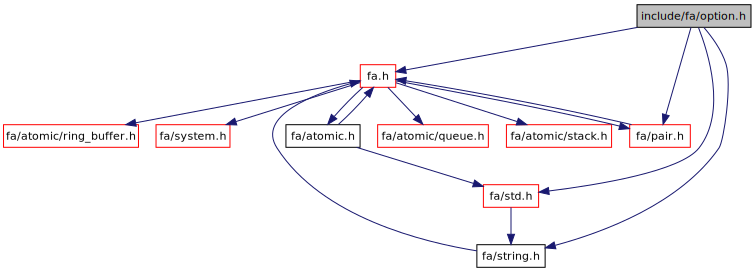
\includegraphics[width=350pt]{option_8h__incl}
\end{center}
\end{figure}
\subsection*{Data Structures}
\begin{DoxyCompactItemize}
\item 
struct \hyperlink{structfa__option__t}{fa\-\_\-option\-\_\-t}
\end{DoxyCompactItemize}
\subsection*{Typedefs}
\begin{DoxyCompactItemize}
\item 
typedef \hyperlink{group___fa_ga915ddeae99ad7568b273d2b876425197}{fa\-\_\-ptr\-\_\-t}($\ast$ \hyperlink{group___fa_option_ga86aa8e13dfaaa7e6870855b204cfe3a0}{fa\-\_\-option\-\_\-parser\-\_\-t} )(char $\ast$)
\end{DoxyCompactItemize}
\subsection*{Functions}
\begin{DoxyCompactItemize}
\item 
\hyperlink{group___fa_ga915ddeae99ad7568b273d2b876425197}{fa\-\_\-ptr\-\_\-t} \hyperlink{group___fa_option_ga9ba72e31cecff0d13f4ad97a76f84c84}{fa\-\_\-option\-\_\-integral} (char $\ast$input)
\begin{DoxyCompactList}\small\item\em Parses integers. \end{DoxyCompactList}\item 
\hyperlink{group___fa_ga915ddeae99ad7568b273d2b876425197}{fa\-\_\-ptr\-\_\-t} \hyperlink{group___fa_option_gaf40e446b8873176ee62f74be2822e1e7}{fa\-\_\-option\-\_\-floating} (char $\ast$input)
\begin{DoxyCompactList}\small\item\em Parses floating-\/point numbers. \end{DoxyCompactList}\item 
\hyperlink{group___fa_ga915ddeae99ad7568b273d2b876425197}{fa\-\_\-ptr\-\_\-t} \hyperlink{group___fa_option_ga8bb94c18d6373f7245188120dcb70562}{fa\-\_\-option\-\_\-string} (char $\ast$input)
\begin{DoxyCompactList}\small\item\em Parses strings. \end{DoxyCompactList}\item 
\hyperlink{group___fa_ga915ddeae99ad7568b273d2b876425197}{fa\-\_\-ptr\-\_\-t} \hyperlink{group___fa_option_gaf46a405a8c9ed29f3f8177e189262425}{fa\-\_\-option\-\_\-failure} (char $\ast$input)
\begin{DoxyCompactList}\small\item\em Always fails. \end{DoxyCompactList}\item 
\hyperlink{group___fa_pair_gac2b2e58c230bac4f8a63ef6c05072680}{fa\-\_\-pair\-\_\-t} \hyperlink{group___fa_option_gaf74fe1a41763c353bf8fa0ed7f4259c6}{fa\-\_\-option\-\_\-parse\-\_\-all} (\hyperlink{structfa__option__t}{fa\-\_\-option\-\_\-t} $\ast$options, int argc, char $\ast$$\ast$argv)
\begin{DoxyCompactList}\small\item\em Parse options according to the given specification (see example above). \end{DoxyCompactList}\item 
void \hyperlink{group___fa_option_ga35db7ce1235a1061817436bedb1b39d6}{fa\-\_\-option\-\_\-show\-\_\-all} (\hyperlink{structfa__option__t}{fa\-\_\-option\-\_\-t} $\ast$options, char $\ast$header)
\begin{DoxyCompactList}\small\item\em Show options according to the given specification (see example above) on the standard output. \end{DoxyCompactList}\item 
\hyperlink{group___fa_pair_gac2b2e58c230bac4f8a63ef6c05072680}{fa\-\_\-pair\-\_\-t} \hyperlink{group___fa_option_ga8a6e4ac1997796f4fab0d787a346fbe8}{fa\-\_\-option\-\_\-parse} (int num\-Options, \hyperlink{structfa__option__t}{fa\-\_\-option\-\_\-t} $\ast$options, int argc, char $\ast$$\ast$argv)
\begin{DoxyCompactList}\small\item\em Parse options according to the given specification (see example above). \end{DoxyCompactList}\item 
void \hyperlink{group___fa_option_gaf0e5db771026f5b3e2e662927e3ed62b}{fa\-\_\-option\-\_\-show} (int num\-Options, \hyperlink{structfa__option__t}{fa\-\_\-option\-\_\-t} $\ast$options, char $\ast$header)
\begin{DoxyCompactList}\small\item\em Show options according to the given specification (see example above) on the standard output. \end{DoxyCompactList}\end{DoxyCompactItemize}

\hypertarget{pair_8h}{\section{include/fa/pair.h File Reference}
\label{pair_8h}\index{include/fa/pair.\-h@{include/fa/pair.\-h}}
}
{\ttfamily \#include $<$fa.\-h$>$}\\*
{\ttfamily \#include $<$fa/list.\-h$>$}\\*
Include dependency graph for pair.\-h\-:\nopagebreak
\begin{figure}[H]
\begin{center}
\leavevmode
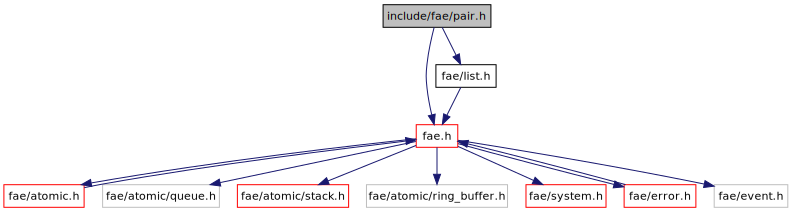
\includegraphics[width=350pt]{pair_8h__incl}
\end{center}
\end{figure}
This graph shows which files directly or indirectly include this file\-:\nopagebreak
\begin{figure}[H]
\begin{center}
\leavevmode
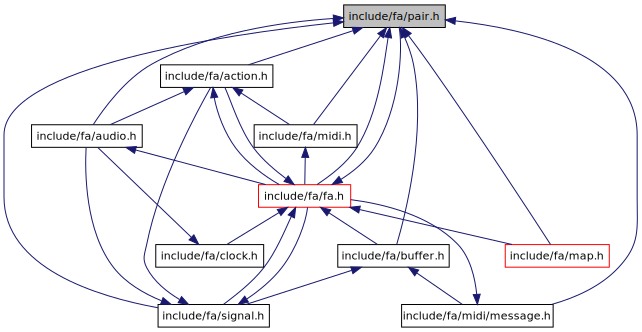
\includegraphics[width=350pt]{pair_8h__dep__incl}
\end{center}
\end{figure}
\subsection*{Data Structures}
\begin{DoxyCompactItemize}
\item 
struct \hyperlink{structfa__pair__struct__t}{fa\-\_\-pair\-\_\-struct\-\_\-t}
\end{DoxyCompactItemize}
\subsection*{Typedefs}
\begin{DoxyCompactItemize}
\item 
typedef struct \-\_\-fa\-\_\-pair\-\_\-t $\ast$ \hyperlink{group___fa_pair_gac2b2e58c230bac4f8a63ef6c05072680}{fa\-\_\-pair\-\_\-t}
\begin{DoxyCompactList}\small\item\em The abstract type of pairs. \end{DoxyCompactList}\end{DoxyCompactItemize}
\subsection*{Functions}
\begin{DoxyCompactItemize}
\item 
\hyperlink{group___fa_pair_gac2b2e58c230bac4f8a63ef6c05072680}{fa\-\_\-pair\-\_\-t} \hyperlink{group___fa_pair_gaea210809bc766ec6aad0580f19f479ac}{fa\-\_\-pair\-\_\-create} (\hyperlink{group___fa_ga915ddeae99ad7568b273d2b876425197}{fa\-\_\-ptr\-\_\-t} ptr, \hyperlink{group___fa_ga915ddeae99ad7568b273d2b876425197}{fa\-\_\-ptr\-\_\-t} ptr\-\_\-)
\begin{DoxyCompactList}\small\item\em Create a new pair. \end{DoxyCompactList}\item 
\hyperlink{group___fa_pair_gac2b2e58c230bac4f8a63ef6c05072680}{fa\-\_\-pair\-\_\-t} \hyperlink{group___fa_pair_gaab0cee4f61bbfa9ba432a5d3b32dd1af}{fa\-\_\-pair\-\_\-read} (\hyperlink{structfa__pair__struct__t}{fa\-\_\-pair\-\_\-struct\-\_\-t} $\ast$)
\begin{DoxyCompactList}\small\item\em Create a pair by reading the components of a structure. \end{DoxyCompactList}\item 
void \hyperlink{group___fa_pair_gab613de74384324db6bba7ad7e6396892}{fa\-\_\-pair\-\_\-write} (\hyperlink{structfa__pair__struct__t}{fa\-\_\-pair\-\_\-struct\-\_\-t} $\ast$, \hyperlink{group___fa_pair_gac2b2e58c230bac4f8a63ef6c05072680}{fa\-\_\-pair\-\_\-t} \hyperlink{util_8h_a40ed40659d2ed7f8712b0fe6ba6edebe}{pair})
\begin{DoxyCompactList}\small\item\em Write the values of a pair to a structure. \end{DoxyCompactList}\item 
\hyperlink{group___fa_pair_gac2b2e58c230bac4f8a63ef6c05072680}{fa\-\_\-pair\-\_\-t} \hyperlink{group___fa_pair_ga2786421b334c7a6dc71b7f25de3369e1}{fa\-\_\-pair\-\_\-copy} (\hyperlink{group___fa_pair_gac2b2e58c230bac4f8a63ef6c05072680}{fa\-\_\-pair\-\_\-t} \hyperlink{util_8h_a40ed40659d2ed7f8712b0fe6ba6edebe}{pair})
\begin{DoxyCompactList}\small\item\em Copy the given pair. \end{DoxyCompactList}\item 
void \hyperlink{group___fa_pair_ga1ac2fe345d109b9ad18335ada198d506}{fa\-\_\-pair\-\_\-destroy} (\hyperlink{group___fa_pair_gac2b2e58c230bac4f8a63ef6c05072680}{fa\-\_\-pair\-\_\-t} \hyperlink{util_8h_a40ed40659d2ed7f8712b0fe6ba6edebe}{pair})
\begin{DoxyCompactList}\small\item\em Destroy the given pair. \end{DoxyCompactList}\item 
void \hyperlink{group___fa_pair_ga7e797364d4d31cd174d974b16627cdfe}{fa\-\_\-pair\-\_\-decons} (\hyperlink{group___fa_ga915ddeae99ad7568b273d2b876425197}{fa\-\_\-ptr\-\_\-t} $\ast$, \hyperlink{group___fa_ga915ddeae99ad7568b273d2b876425197}{fa\-\_\-ptr\-\_\-t} $\ast$, \hyperlink{group___fa_pair_gac2b2e58c230bac4f8a63ef6c05072680}{fa\-\_\-pair\-\_\-t} \hyperlink{util_8h_a40ed40659d2ed7f8712b0fe6ba6edebe}{pair})
\begin{DoxyCompactList}\small\item\em Get the first and second components of the given pair. \end{DoxyCompactList}\item 
\hyperlink{group___fa_ga915ddeae99ad7568b273d2b876425197}{fa\-\_\-ptr\-\_\-t} \hyperlink{group___fa_pair_gaa61373d5c0648b4670ff51c483c2977d}{fa\-\_\-pair\-\_\-first} (\hyperlink{group___fa_pair_gac2b2e58c230bac4f8a63ef6c05072680}{fa\-\_\-pair\-\_\-t} \hyperlink{util_8h_a40ed40659d2ed7f8712b0fe6ba6edebe}{pair})
\begin{DoxyCompactList}\small\item\em Get the first component of the given pair. \end{DoxyCompactList}\item 
\hyperlink{group___fa_ga915ddeae99ad7568b273d2b876425197}{fa\-\_\-ptr\-\_\-t} \hyperlink{group___fa_pair_ga4c681f429b7677e05f6f5aadc0d1c18d}{fa\-\_\-pair\-\_\-second} (\hyperlink{group___fa_pair_gac2b2e58c230bac4f8a63ef6c05072680}{fa\-\_\-pair\-\_\-t} \hyperlink{util_8h_a40ed40659d2ed7f8712b0fe6ba6edebe}{pair})
\begin{DoxyCompactList}\small\item\em Get the second component of the given pair. \end{DoxyCompactList}\item 
\hyperlink{group___fa_pair_gac2b2e58c230bac4f8a63ef6c05072680}{fa\-\_\-pair\-\_\-t} \hyperlink{group___fa_pair_gaf0c419c071f484dbd09e9c33b03d1a8c}{fa\-\_\-pair\-\_\-duplicate} (\hyperlink{group___fa_ga915ddeae99ad7568b273d2b876425197}{fa\-\_\-ptr\-\_\-t} ptr)
\begin{DoxyCompactList}\small\item\em Return a pair containing the given value as both its left and right component. \end{DoxyCompactList}\item 
\hyperlink{group___fa_pair_gac2b2e58c230bac4f8a63ef6c05072680}{fa\-\_\-pair\-\_\-t} \hyperlink{group___fa_pair_gab905200bb654bfd3cfc36c2adf4383fd}{fa\-\_\-pair\-\_\-swap} (\hyperlink{group___fa_pair_gac2b2e58c230bac4f8a63ef6c05072680}{fa\-\_\-pair\-\_\-t} \hyperlink{util_8h_a40ed40659d2ed7f8712b0fe6ba6edebe}{pair})
\begin{DoxyCompactList}\small\item\em Swap the components of the given pair. \end{DoxyCompactList}\item 
\hyperlink{group___fa_pair_gac2b2e58c230bac4f8a63ef6c05072680}{fa\-\_\-pair\-\_\-t} \hyperlink{group___fa_pair_gaa8b9eb2a799ec3993b5f9127ed511188}{fa\-\_\-pair\-\_\-assoc} (\hyperlink{group___fa_pair_gac2b2e58c230bac4f8a63ef6c05072680}{fa\-\_\-pair\-\_\-t} \hyperlink{util_8h_a40ed40659d2ed7f8712b0fe6ba6edebe}{pair})
\begin{DoxyCompactList}\small\item\em Return the left-\/associated version of the given nested pair. \end{DoxyCompactList}\item 
\hyperlink{group___fa_pair_gac2b2e58c230bac4f8a63ef6c05072680}{fa\-\_\-pair\-\_\-t} \hyperlink{group___fa_pair_gaff4d8830c9436aa7fa6b0ca0a99c06f8}{fa\-\_\-pair\-\_\-unassoc} (\hyperlink{group___fa_pair_gac2b2e58c230bac4f8a63ef6c05072680}{fa\-\_\-pair\-\_\-t} \hyperlink{util_8h_a40ed40659d2ed7f8712b0fe6ba6edebe}{pair})
\begin{DoxyCompactList}\small\item\em Return the right-\/associated version of the given nested pair. \end{DoxyCompactList}\item 
\hyperlink{group___fa_list_ga35ecb12ab934ded0cce0bcf28e3bc5d2}{fa\-\_\-list\-\_\-t} \hyperlink{group___fa_pair_gac21e1f6a5da734bf51986b7ab413c810}{fa\-\_\-pair\-\_\-to\-\_\-list} (\hyperlink{group___fa_pair_gac2b2e58c230bac4f8a63ef6c05072680}{fa\-\_\-pair\-\_\-t} \hyperlink{util_8h_a40ed40659d2ed7f8712b0fe6ba6edebe}{pair})
\begin{DoxyCompactList}\small\item\em Convert a pair to a list of two elements. \end{DoxyCompactList}\end{DoxyCompactItemize}

\hypertarget{priority__queue_8h}{\section{include/fa/priority\-\_\-queue.h File Reference}
\label{priority__queue_8h}\index{include/fa/priority\-\_\-queue.\-h@{include/fa/priority\-\_\-queue.\-h}}
}
{\ttfamily \#include $<$fa.\-h$>$}\\*
Include dependency graph for priority\-\_\-queue.\-h\-:\nopagebreak
\begin{figure}[H]
\begin{center}
\leavevmode
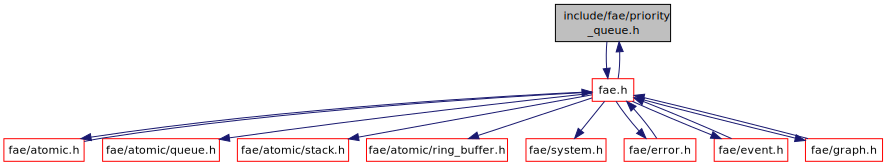
\includegraphics[width=350pt]{priority__queue_8h__incl}
\end{center}
\end{figure}
This graph shows which files directly or indirectly include this file\-:\nopagebreak
\begin{figure}[H]
\begin{center}
\leavevmode
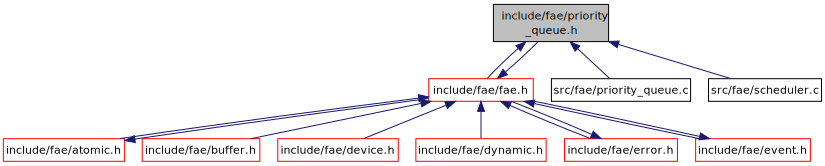
\includegraphics[width=350pt]{priority__queue_8h__dep__incl}
\end{center}
\end{figure}
\subsection*{Typedefs}
\begin{DoxyCompactItemize}
\item 
typedef struct \\*
\-\_\-fa\-\_\-priority\-\_\-queue\-\_\-t $\ast$ \hyperlink{group___fa_priority_queue_ga4363f15ce2b05e7c4af410cd6509ef5a}{fa\-\_\-priority\-\_\-queue\-\_\-t}
\end{DoxyCompactItemize}
\subsection*{Functions}
\begin{DoxyCompactItemize}
\item 
\hyperlink{group___fa_priority_queue_ga4363f15ce2b05e7c4af410cd6509ef5a}{fa\-\_\-priority\-\_\-queue\-\_\-t} \hyperlink{group___fa_priority_queue_gaa1699e0b582ae2989a2d56e494838e30}{fa\-\_\-priority\-\_\-queue\-\_\-empty} ()
\begin{DoxyCompactList}\small\item\em Create an empty queue. \end{DoxyCompactList}\item 
\hyperlink{group___fa_priority_queue_ga4363f15ce2b05e7c4af410cd6509ef5a}{fa\-\_\-priority\-\_\-queue\-\_\-t} \hyperlink{group___fa_priority_queue_gaaabe71c5b718985a2a9b2859fc7f6ea8}{fa\-\_\-priority\-\_\-queue\-\_\-single} (\hyperlink{group___fa_ga915ddeae99ad7568b273d2b876425197}{fa\-\_\-ptr\-\_\-t} ptr)
\begin{DoxyCompactList}\small\item\em Create an queue containing a single element. \end{DoxyCompactList}\item 
void \hyperlink{group___fa_priority_queue_gacbdd365a4a621b0458929645f27a016d}{fa\-\_\-priority\-\_\-queue\-\_\-destroy} (\hyperlink{group___fa_priority_queue_ga4363f15ce2b05e7c4af410cd6509ef5a}{fa\-\_\-priority\-\_\-queue\-\_\-t} priority\-Queue)
\begin{DoxyCompactList}\small\item\em Destroy the given queue. \end{DoxyCompactList}\item 
void \hyperlink{group___fa_priority_queue_ga5efe0e7da7de5cdbd2a88103922e3b69}{fa\-\_\-priority\-\_\-queue\-\_\-merge} (\hyperlink{group___fa_priority_queue_ga4363f15ce2b05e7c4af410cd6509ef5a}{fa\-\_\-priority\-\_\-queue\-\_\-t} priority\-Queue, \hyperlink{group___fa_priority_queue_ga4363f15ce2b05e7c4af410cd6509ef5a}{fa\-\_\-priority\-\_\-queue\-\_\-t} priority\-Queue\-\_\-)
\begin{DoxyCompactList}\small\item\em Merge the two given queues into the first. \end{DoxyCompactList}\item 
void \hyperlink{group___fa_priority_queue_ga579f5579ab78eb82223b769f4a56933f}{fa\-\_\-priority\-\_\-queue\-\_\-insert} (\hyperlink{group___fa_ga915ddeae99ad7568b273d2b876425197}{fa\-\_\-ptr\-\_\-t} ptr, \hyperlink{group___fa_priority_queue_ga4363f15ce2b05e7c4af410cd6509ef5a}{fa\-\_\-priority\-\_\-queue\-\_\-t} priority\-Queue)
\begin{DoxyCompactList}\small\item\em Insert the given element into the given queue. \end{DoxyCompactList}\item 
\hyperlink{group___fa_ga915ddeae99ad7568b273d2b876425197}{fa\-\_\-ptr\-\_\-t} \hyperlink{group___fa_priority_queue_ga07dad7064b633feff9b9f8543173dcc0}{fa\-\_\-priority\-\_\-queue\-\_\-peek} (\hyperlink{group___fa_priority_queue_ga4363f15ce2b05e7c4af410cd6509ef5a}{fa\-\_\-priority\-\_\-queue\-\_\-t} priority\-Queue)
\begin{DoxyCompactList}\small\item\em Returns the top-\/most element in the given queue, if any. \end{DoxyCompactList}\item 
\hyperlink{group___fa_ga915ddeae99ad7568b273d2b876425197}{fa\-\_\-ptr\-\_\-t} \hyperlink{group___fa_priority_queue_gac2ec9dbd70a479fd54c857f1de8d0902}{fa\-\_\-priority\-\_\-queue\-\_\-pop} (\hyperlink{group___fa_priority_queue_ga4363f15ce2b05e7c4af410cd6509ef5a}{fa\-\_\-priority\-\_\-queue\-\_\-t} priority\-Queue)
\begin{DoxyCompactList}\small\item\em Returns the top-\/most element and remove it from the queue. \end{DoxyCompactList}\end{DoxyCompactItemize}

\hypertarget{ratio_8h}{\section{include/fa/ratio.h File Reference}
\label{ratio_8h}\index{include/fa/ratio.\-h@{include/fa/ratio.\-h}}
}
{\ttfamily \#include $<$fa/std.\-h$>$}\\*
Include dependency graph for ratio.\-h\-:\nopagebreak
\begin{figure}[H]
\begin{center}
\leavevmode
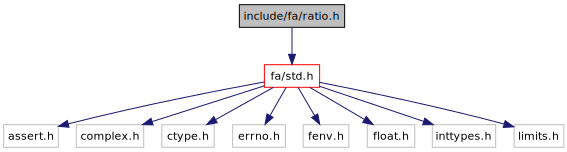
\includegraphics[width=350pt]{ratio_8h__incl}
\end{center}
\end{figure}
This graph shows which files directly or indirectly include this file\-:\nopagebreak
\begin{figure}[H]
\begin{center}
\leavevmode
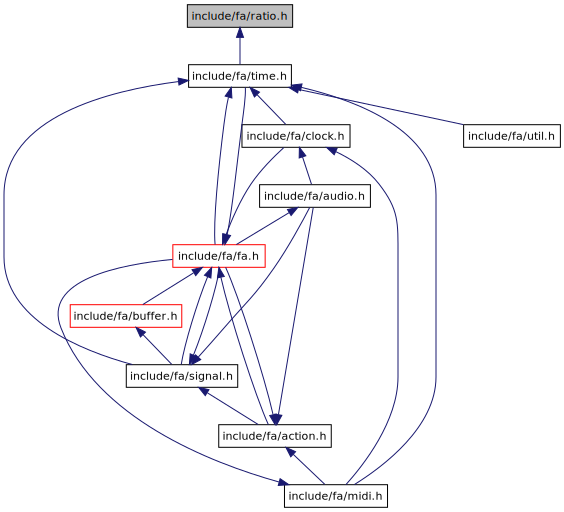
\includegraphics[width=350pt]{ratio_8h__dep__incl}
\end{center}
\end{figure}
\subsection*{Typedefs}
\begin{DoxyCompactItemize}
\item 
typedef int32\-\_\-t \hyperlink{group___fa_ratio_ga6d6962b946d96535558e341030f16e07}{fa\-\_\-ratio\-\_\-num\-\_\-t}
\item 
typedef int32\-\_\-t \hyperlink{group___fa_ratio_ga18626f0c26ea1666ce0725605044cfa1}{fa\-\_\-ratio\-\_\-denom\-\_\-t}
\item 
typedef struct \-\_\-fa\-\_\-ratio\-\_\-t $\ast$ \hyperlink{group___fa_ratio_gaf3b37b5fdfcccb6283b7ac806c72b273}{fa\-\_\-ratio\-\_\-t}
\begin{DoxyCompactList}\small\item\em A rational number. \end{DoxyCompactList}\end{DoxyCompactItemize}
\subsection*{Functions}
\begin{DoxyCompactItemize}
\item 
\hyperlink{group___fa_ratio_gaf3b37b5fdfcccb6283b7ac806c72b273}{fa\-\_\-ratio\-\_\-t} \hyperlink{group___fa_ratio_ga3ab0d3fea73d05b4173e066f954389a5}{fa\-\_\-ratio\-\_\-create} (\hyperlink{group___fa_ratio_ga6d6962b946d96535558e341030f16e07}{fa\-\_\-ratio\-\_\-num\-\_\-t} num, \hyperlink{group___fa_ratio_ga18626f0c26ea1666ce0725605044cfa1}{fa\-\_\-ratio\-\_\-denom\-\_\-t} denom)
\begin{DoxyCompactList}\small\item\em Create a rational number. \end{DoxyCompactList}\item 
\hyperlink{group___fa_ratio_ga6d6962b946d96535558e341030f16e07}{fa\-\_\-ratio\-\_\-num\-\_\-t} \hyperlink{group___fa_ratio_gaa94661f5ff09ed1a547f870f6e1c5a9b}{fa\-\_\-ratio\-\_\-num} (\hyperlink{group___fa_ratio_gaf3b37b5fdfcccb6283b7ac806c72b273}{fa\-\_\-ratio\-\_\-t} \hyperlink{util_8h_a866d3cbbee2679ec3c34f27a256445de}{ratio})
\begin{DoxyCompactList}\small\item\em Return the numerator of the given rational number. \end{DoxyCompactList}\item 
\hyperlink{group___fa_ratio_ga18626f0c26ea1666ce0725605044cfa1}{fa\-\_\-ratio\-\_\-denom\-\_\-t} \hyperlink{group___fa_ratio_ga71fb6b16111090ebef75fce0a62eb234}{fa\-\_\-ratio\-\_\-denom} (\hyperlink{group___fa_ratio_gaf3b37b5fdfcccb6283b7ac806c72b273}{fa\-\_\-ratio\-\_\-t} \hyperlink{util_8h_a866d3cbbee2679ec3c34f27a256445de}{ratio})
\begin{DoxyCompactList}\small\item\em Return the denominator of the given rational number. \end{DoxyCompactList}\item 
void \hyperlink{group___fa_ratio_gacb1ec6f18e009d96c398f83e7a507270}{fa\-\_\-ratio\-\_\-match} (\hyperlink{group___fa_ratio_gaf3b37b5fdfcccb6283b7ac806c72b273}{fa\-\_\-ratio\-\_\-t} \hyperlink{util_8h_a866d3cbbee2679ec3c34f27a256445de}{ratio}, \hyperlink{group___fa_ratio_ga6d6962b946d96535558e341030f16e07}{fa\-\_\-ratio\-\_\-num\-\_\-t} $\ast$, \hyperlink{group___fa_ratio_ga18626f0c26ea1666ce0725605044cfa1}{fa\-\_\-ratio\-\_\-denom\-\_\-t} $\ast$)
\begin{DoxyCompactList}\small\item\em Destruct the given rational number, writing its numerator and denominator to the given locations. \end{DoxyCompactList}\item 
\hyperlink{group___fa_ratio_gaf3b37b5fdfcccb6283b7ac806c72b273}{fa\-\_\-ratio\-\_\-t} \hyperlink{group___fa_ratio_ga240d745928d4f3ea0f03930617580f62}{fa\-\_\-ratio\-\_\-copy} (\hyperlink{group___fa_ratio_gaf3b37b5fdfcccb6283b7ac806c72b273}{fa\-\_\-ratio\-\_\-t} \hyperlink{util_8h_a866d3cbbee2679ec3c34f27a256445de}{ratio})
\begin{DoxyCompactList}\small\item\em Copy a rational number. \end{DoxyCompactList}\item 
void \hyperlink{group___fa_ratio_gaa65ebd7b8a36f340bf5d54ff8d14738e}{fa\-\_\-ratio\-\_\-destroy} (\hyperlink{group___fa_ratio_gaf3b37b5fdfcccb6283b7ac806c72b273}{fa\-\_\-ratio\-\_\-t} \hyperlink{util_8h_a866d3cbbee2679ec3c34f27a256445de}{ratio})
\begin{DoxyCompactList}\small\item\em Destroy a rational number. \end{DoxyCompactList}\item 
\hyperlink{group___fa_ratio_gaf3b37b5fdfcccb6283b7ac806c72b273}{fa\-\_\-ratio\-\_\-t} \hyperlink{group___fa_ratio_ga6f21aa6cbc2216a1277f2158968ce52b}{fa\-\_\-ratio\-\_\-add} (\hyperlink{group___fa_ratio_gaf3b37b5fdfcccb6283b7ac806c72b273}{fa\-\_\-ratio\-\_\-t} \hyperlink{util_8h_a866d3cbbee2679ec3c34f27a256445de}{ratio}, \hyperlink{group___fa_ratio_gaf3b37b5fdfcccb6283b7ac806c72b273}{fa\-\_\-ratio\-\_\-t} ratio\-\_\-)
\begin{DoxyCompactList}\small\item\em Add the given rational numbers. \end{DoxyCompactList}\item 
\hyperlink{group___fa_ratio_gaf3b37b5fdfcccb6283b7ac806c72b273}{fa\-\_\-ratio\-\_\-t} \hyperlink{group___fa_ratio_ga4532996b003dc8a628053dd8d159cf82}{fa\-\_\-ratio\-\_\-subtract} (\hyperlink{group___fa_ratio_gaf3b37b5fdfcccb6283b7ac806c72b273}{fa\-\_\-ratio\-\_\-t} \hyperlink{util_8h_a866d3cbbee2679ec3c34f27a256445de}{ratio}, \hyperlink{group___fa_ratio_gaf3b37b5fdfcccb6283b7ac806c72b273}{fa\-\_\-ratio\-\_\-t} ratio\-\_\-)
\begin{DoxyCompactList}\small\item\em Subtract the given rational numbers. \end{DoxyCompactList}\item 
\hyperlink{group___fa_ratio_gaf3b37b5fdfcccb6283b7ac806c72b273}{fa\-\_\-ratio\-\_\-t} \hyperlink{group___fa_ratio_gaeeef9bb9a4a888e53e7fbe09ff5c5dd0}{fa\-\_\-ratio\-\_\-multiply} (\hyperlink{group___fa_ratio_gaf3b37b5fdfcccb6283b7ac806c72b273}{fa\-\_\-ratio\-\_\-t} \hyperlink{util_8h_a866d3cbbee2679ec3c34f27a256445de}{ratio}, \hyperlink{group___fa_ratio_gaf3b37b5fdfcccb6283b7ac806c72b273}{fa\-\_\-ratio\-\_\-t} ratio\-\_\-)
\begin{DoxyCompactList}\small\item\em Multiply the given rational numbers. \end{DoxyCompactList}\item 
\hyperlink{group___fa_ratio_gaf3b37b5fdfcccb6283b7ac806c72b273}{fa\-\_\-ratio\-\_\-t} \hyperlink{group___fa_ratio_ga5995de6035f8f7f95c645dfd6d1b3297}{fa\-\_\-ratio\-\_\-divide} (\hyperlink{group___fa_ratio_gaf3b37b5fdfcccb6283b7ac806c72b273}{fa\-\_\-ratio\-\_\-t} \hyperlink{util_8h_a866d3cbbee2679ec3c34f27a256445de}{ratio}, \hyperlink{group___fa_ratio_gaf3b37b5fdfcccb6283b7ac806c72b273}{fa\-\_\-ratio\-\_\-t} ratio\-\_\-)
\begin{DoxyCompactList}\small\item\em Divide the given rational numbers. \end{DoxyCompactList}\item 
\hyperlink{group___fa_ratio_gaf3b37b5fdfcccb6283b7ac806c72b273}{fa\-\_\-ratio\-\_\-t} \hyperlink{group___fa_ratio_ga7c72bad7eef5ca15eb888b08ed744ed0}{fa\-\_\-ratio\-\_\-succ} (\hyperlink{group___fa_ratio_gaf3b37b5fdfcccb6283b7ac806c72b273}{fa\-\_\-ratio\-\_\-t} \hyperlink{util_8h_a866d3cbbee2679ec3c34f27a256445de}{ratio})
\begin{DoxyCompactList}\small\item\em Return the successor of the given rational number. \end{DoxyCompactList}\item 
\hyperlink{group___fa_ratio_gaf3b37b5fdfcccb6283b7ac806c72b273}{fa\-\_\-ratio\-\_\-t} \hyperlink{group___fa_ratio_ga78052a323d41d5d76a526e1e19ba0eb2}{fa\-\_\-ratio\-\_\-pred} (\hyperlink{group___fa_ratio_gaf3b37b5fdfcccb6283b7ac806c72b273}{fa\-\_\-ratio\-\_\-t} \hyperlink{util_8h_a866d3cbbee2679ec3c34f27a256445de}{ratio})
\begin{DoxyCompactList}\small\item\em Return the predecessor of the given rational number. \end{DoxyCompactList}\item 
\hyperlink{group___fa_ratio_gaf3b37b5fdfcccb6283b7ac806c72b273}{fa\-\_\-ratio\-\_\-t} \hyperlink{group___fa_ratio_ga39bc43bc50d936309bf763b6903249bd}{fa\-\_\-ratio\-\_\-negate} (\hyperlink{group___fa_ratio_gaf3b37b5fdfcccb6283b7ac806c72b273}{fa\-\_\-ratio\-\_\-t} \hyperlink{util_8h_a866d3cbbee2679ec3c34f27a256445de}{ratio})
\begin{DoxyCompactList}\small\item\em Negate the given rational number. \end{DoxyCompactList}\item 
\hyperlink{group___fa_ratio_gaf3b37b5fdfcccb6283b7ac806c72b273}{fa\-\_\-ratio\-\_\-t} \hyperlink{group___fa_ratio_gae2a0b5d0ca551b62a4a8edc6b399b742}{fa\-\_\-ratio\-\_\-recip} (\hyperlink{group___fa_ratio_gaf3b37b5fdfcccb6283b7ac806c72b273}{fa\-\_\-ratio\-\_\-t} \hyperlink{util_8h_a866d3cbbee2679ec3c34f27a256445de}{ratio})
\begin{DoxyCompactList}\small\item\em Invert the given rational number. \end{DoxyCompactList}\item 
\hyperlink{group___fa_ratio_gaf3b37b5fdfcccb6283b7ac806c72b273}{fa\-\_\-ratio\-\_\-t} \hyperlink{group___fa_ratio_gae3545b10373eeba8414a490e5d9d0ec8}{fa\-\_\-ratio\-\_\-absolute} (\hyperlink{group___fa_ratio_gaf3b37b5fdfcccb6283b7ac806c72b273}{fa\-\_\-ratio\-\_\-t} \hyperlink{util_8h_a866d3cbbee2679ec3c34f27a256445de}{ratio})
\begin{DoxyCompactList}\small\item\em Return the absolute value of the given rational number. \end{DoxyCompactList}\item 
\hyperlink{group___fa_ratio_gaf3b37b5fdfcccb6283b7ac806c72b273}{fa\-\_\-ratio\-\_\-t} \hyperlink{group___fa_ratio_gad477d6485fd4e6ff3bca8bda977447ff}{fa\-\_\-ratio\-\_\-normalize} (\hyperlink{group___fa_ratio_gaf3b37b5fdfcccb6283b7ac806c72b273}{fa\-\_\-ratio\-\_\-t} \hyperlink{util_8h_a866d3cbbee2679ec3c34f27a256445de}{ratio})
\begin{DoxyCompactList}\small\item\em Normalize the given rational number. \end{DoxyCompactList}\item 
void \hyperlink{group___fa_ratio_ga13dc172c048dcd34c04aedd20f0fe1d6}{fa\-\_\-ratio\-\_\-to\-\_\-mixed} (\hyperlink{group___fa_ratio_gaf3b37b5fdfcccb6283b7ac806c72b273}{fa\-\_\-ratio\-\_\-t} \hyperlink{util_8h_a866d3cbbee2679ec3c34f27a256445de}{ratio}, \hyperlink{group___fa_ratio_ga6d6962b946d96535558e341030f16e07}{fa\-\_\-ratio\-\_\-num\-\_\-t} $\ast$, \hyperlink{group___fa_ratio_gaf3b37b5fdfcccb6283b7ac806c72b273}{fa\-\_\-ratio\-\_\-t} $\ast$)
\begin{DoxyCompactList}\small\item\em Convert the given rational number to mixed form. \end{DoxyCompactList}\end{DoxyCompactItemize}

\hypertarget{signal_8h}{\section{include/fa/signal.h File Reference}
\label{signal_8h}\index{include/fa/signal.\-h@{include/fa/signal.\-h}}
}
{\ttfamily \#include $<$fa.\-h$>$}\\*
{\ttfamily \#include $<$fa/pair.\-h$>$}\\*
{\ttfamily \#include $<$fa/time.\-h$>$}\\*
{\ttfamily \#include $<$fa/buffer.\-h$>$}\\*
{\ttfamily \#include $<$fa/atomic/ring\-\_\-buffer.\-h$>$}\\*
Include dependency graph for signal.\-h\-:\nopagebreak
\begin{figure}[H]
\begin{center}
\leavevmode
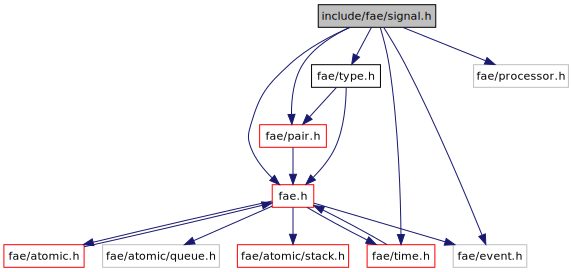
\includegraphics[width=350pt]{signal_8h__incl}
\end{center}
\end{figure}
This graph shows which files directly or indirectly include this file\-:\nopagebreak
\begin{figure}[H]
\begin{center}
\leavevmode
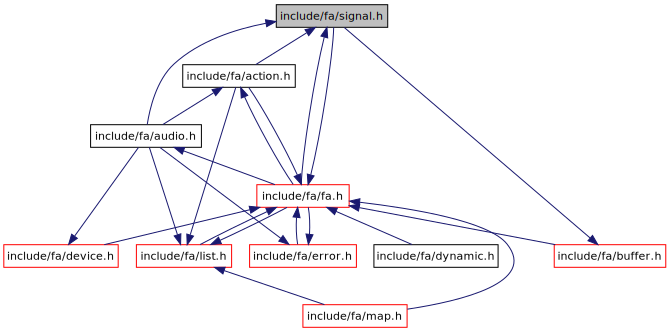
\includegraphics[width=350pt]{signal_8h__dep__incl}
\end{center}
\end{figure}
\subsection*{Data Structures}
\begin{DoxyCompactItemize}
\item 
struct \hyperlink{structfa__signal__state__t}{fa\-\_\-signal\-\_\-state\-\_\-t}
\item 
struct \hyperlink{structfa__signal__custom__processor__t}{fa\-\_\-signal\-\_\-custom\-\_\-processor\-\_\-t}
\end{DoxyCompactItemize}
\subsection*{Typedefs}
\begin{DoxyCompactItemize}
\item 
typedef struct \-\_\-fa\-\_\-signal\-\_\-t $\ast$ \hyperlink{group___fa_signal_gac5c72f160cd6e93a6783551627b166e5}{fa\-\_\-signal\-\_\-t}
\begin{DoxyCompactList}\small\item\em The abstract type of signals. \end{DoxyCompactList}\item 
typedef \hyperlink{group___fa_signal_gac5c72f160cd6e93a6783551627b166e5}{fa\-\_\-signal\-\_\-t}($\ast$ \hyperlink{group___fa_signal_gaa1f5df5ce102da5b837ccfee4632c7b4}{fa\-\_\-signal\-\_\-unary\-\_\-signal\-\_\-t} )(\hyperlink{group___fa_ga915ddeae99ad7568b273d2b876425197}{fa\-\_\-ptr\-\_\-t}, \hyperlink{group___fa_signal_gac5c72f160cd6e93a6783551627b166e5}{fa\-\_\-signal\-\_\-t})
\begin{DoxyCompactList}\small\item\em Like fa\-\_\-unary\-\_\-t, but speficied on signals. \end{DoxyCompactList}\item 
typedef double($\ast$ \hyperlink{group___fa_signal_gaced7eb8d67eb2fe39927934c4abc7255}{fa\-\_\-signal\-\_\-unary\-\_\-double\-\_\-t} )(\hyperlink{group___fa_ga915ddeae99ad7568b273d2b876425197}{fa\-\_\-ptr\-\_\-t}, double)
\begin{DoxyCompactList}\small\item\em Like fa\-\_\-unary\-\_\-t, but speficied on doubles. \end{DoxyCompactList}\item 
typedef double($\ast$ \hyperlink{group___fa_signal_ga7593031729bc7c15d5da9a06ce3eaf4a}{fa\-\_\-signal\-\_\-binary\-\_\-double\-\_\-t} )(\hyperlink{group___fa_ga915ddeae99ad7568b273d2b876425197}{fa\-\_\-ptr\-\_\-t}, double, double)
\begin{DoxyCompactList}\small\item\em Like fa\-\_\-binary\-\_\-t, but speficied on doubles. \end{DoxyCompactList}\item 
typedef \hyperlink{group___fa_string_gacada63033b77bc6c39fa632ae199349b}{fa\-\_\-string\-\_\-t} \hyperlink{group___fa_signal_gabb3471c5e8fbc3ab8657964de4200d37}{fa\-\_\-signal\-\_\-name\-\_\-t}
\item 
typedef \hyperlink{group___fa_ga915ddeae99ad7568b273d2b876425197}{fa\-\_\-ptr\-\_\-t} \hyperlink{group___fa_signal_ga655db48baa224e32e8fc00f33179b46e}{fa\-\_\-signal\-\_\-message\-\_\-t}
\end{DoxyCompactItemize}
\subsection*{Functions}
\begin{DoxyCompactItemize}
\item 
\hyperlink{group___fa_signal_gac5c72f160cd6e93a6783551627b166e5}{fa\-\_\-signal\-\_\-t} \hyperlink{group___fa_signal_ga1884836b27b28547fcccdda085c6e947}{fa\-\_\-signal\-\_\-time} ()
\begin{DoxyCompactList}\small\item\em Returns a signal representing the elapsed time in seconds. \end{DoxyCompactList}\item 
\hyperlink{group___fa_signal_gac5c72f160cd6e93a6783551627b166e5}{fa\-\_\-signal\-\_\-t} \hyperlink{group___fa_signal_ga3e53efe955d4c0c931b6440765936117}{fa\-\_\-signal\-\_\-random} ()
\begin{DoxyCompactList}\small\item\em Returns a signal representing white noise. \end{DoxyCompactList}\item 
\hyperlink{group___fa_signal_gac5c72f160cd6e93a6783551627b166e5}{fa\-\_\-signal\-\_\-t} \hyperlink{group___fa_signal_ga7df7e39eda3a5207258d91c9a9658dcc}{fa\-\_\-signal\-\_\-constant} (double double\-\_\-)
\begin{DoxyCompactList}\small\item\em Returns a signal representing the given constant value. \end{DoxyCompactList}\item 
\hyperlink{group___fa_signal_gac5c72f160cd6e93a6783551627b166e5}{fa\-\_\-signal\-\_\-t} \hyperlink{group___fa_signal_gafd7d235d7ee945bf34227c94f9383cfc}{fa\-\_\-signal\-\_\-lift} (\hyperlink{group___fa_string_gacada63033b77bc6c39fa632ae199349b}{fa\-\_\-string\-\_\-t} \hyperlink{util_8h_a41106000aac73b61e4fc2ef9dd39a603}{string}, \hyperlink{group___fa_signal_gaced7eb8d67eb2fe39927934c4abc7255}{fa\-\_\-signal\-\_\-unary\-\_\-double\-\_\-t} unary\-Double, \hyperlink{group___fa_ga915ddeae99ad7568b273d2b876425197}{fa\-\_\-ptr\-\_\-t} ptr, \hyperlink{group___fa_signal_gac5c72f160cd6e93a6783551627b166e5}{fa\-\_\-signal\-\_\-t} signal)
\begin{DoxyCompactList}\small\item\em Returns a signal that applies the given function to output of the given signal. \end{DoxyCompactList}\item 
\hyperlink{group___fa_signal_gac5c72f160cd6e93a6783551627b166e5}{fa\-\_\-signal\-\_\-t} \hyperlink{group___fa_signal_gaed576fde42afc5f3298a6564c2d2595e}{fa\-\_\-signal\-\_\-lift2} (\hyperlink{group___fa_string_gacada63033b77bc6c39fa632ae199349b}{fa\-\_\-string\-\_\-t} \hyperlink{util_8h_a41106000aac73b61e4fc2ef9dd39a603}{string}, \hyperlink{group___fa_signal_ga7593031729bc7c15d5da9a06ce3eaf4a}{fa\-\_\-signal\-\_\-binary\-\_\-double\-\_\-t} binary\-Double, \hyperlink{group___fa_ga915ddeae99ad7568b273d2b876425197}{fa\-\_\-ptr\-\_\-t} ptr, \hyperlink{group___fa_signal_gac5c72f160cd6e93a6783551627b166e5}{fa\-\_\-signal\-\_\-t} signal, \hyperlink{group___fa_signal_gac5c72f160cd6e93a6783551627b166e5}{fa\-\_\-signal\-\_\-t} signal\-\_\-)
\begin{DoxyCompactList}\small\item\em Returns a signal that applies the given function to output of the given signals. \end{DoxyCompactList}\item 
\hyperlink{group___fa_signal_gac5c72f160cd6e93a6783551627b166e5}{fa\-\_\-signal\-\_\-t} \hyperlink{group___fa_signal_gae940e689d1f147fb76d4272ad3f2a5cc}{fa\-\_\-signal\-\_\-loop} (\hyperlink{group___fa_signal_gaa1f5df5ce102da5b837ccfee4632c7b4}{fa\-\_\-signal\-\_\-unary\-\_\-signal\-\_\-t} unary\-Signal, \hyperlink{group___fa_ga915ddeae99ad7568b273d2b876425197}{fa\-\_\-ptr\-\_\-t} ptr)
\begin{DoxyCompactList}\small\item\em Returns a signal that closes over the given signal function in a feedback loop. \end{DoxyCompactList}\item 
\hyperlink{group___fa_signal_gac5c72f160cd6e93a6783551627b166e5}{fa\-\_\-signal\-\_\-t} \hyperlink{group___fa_signal_ga725db73f7f62b61ed9b34849f2438a07}{fa\-\_\-signal\-\_\-delay} (int int\-\_\-, \hyperlink{group___fa_signal_gac5c72f160cd6e93a6783551627b166e5}{fa\-\_\-signal\-\_\-t} signal)
\begin{DoxyCompactList}\small\item\em Returns a signal that delays the given signal by the given number of samples. \end{DoxyCompactList}\item 
\hyperlink{group___fa_signal_gac5c72f160cd6e93a6783551627b166e5}{fa\-\_\-signal\-\_\-t} \hyperlink{group___fa_signal_gac7b771cb4c1e2e9756b2c63f5d5b6e1b}{fa\-\_\-signal\-\_\-custom} (\hyperlink{structfa__signal__custom__processor__t}{fa\-\_\-signal\-\_\-custom\-\_\-processor\-\_\-t} $\ast$, \hyperlink{group___fa_signal_gac5c72f160cd6e93a6783551627b166e5}{fa\-\_\-signal\-\_\-t} signal)
\begin{DoxyCompactList}\small\item\em Add a custom processor to be executed with the given signal. \end{DoxyCompactList}\item 
\hyperlink{group___fa_signal_gac5c72f160cd6e93a6783551627b166e5}{fa\-\_\-signal\-\_\-t} \hyperlink{group___fa_signal_gafd39f63693a025305682c02bd84a279b}{fa\-\_\-signal\-\_\-input} (int int\-\_\-)
\begin{DoxyCompactList}\small\item\em The primitive input signal, reading from the bus of the given number. \end{DoxyCompactList}\item 
\hyperlink{group___fa_signal_gac5c72f160cd6e93a6783551627b166e5}{fa\-\_\-signal\-\_\-t} \hyperlink{group___fa_signal_ga48817a0a198589535a59b8f39fa6cff0}{fa\-\_\-signal\-\_\-output} (int int\-\_\-, int int\-\_\-\-\_\-, \hyperlink{group___fa_signal_gac5c72f160cd6e93a6783551627b166e5}{fa\-\_\-signal\-\_\-t} signal)
\begin{DoxyCompactList}\small\item\em The primitive output signal, writing to the bus of the given number and returning the written value. \end{DoxyCompactList}\item 
\hyperlink{group___fa_signal_gac5c72f160cd6e93a6783551627b166e5}{fa\-\_\-signal\-\_\-t} \hyperlink{group___fa_signal_gadf564a32b3dc1cd0e9c583f01fecb6de}{fa\-\_\-signal\-\_\-former} (\hyperlink{group___fa_signal_gac5c72f160cd6e93a6783551627b166e5}{fa\-\_\-signal\-\_\-t} signal, \hyperlink{group___fa_signal_gac5c72f160cd6e93a6783551627b166e5}{fa\-\_\-signal\-\_\-t} signal\-\_\-)
\begin{DoxyCompactList}\small\item\em Returns a signal that evaluates both of the given signal, and the result of the first. \end{DoxyCompactList}\item 
\hyperlink{group___fa_signal_gac5c72f160cd6e93a6783551627b166e5}{fa\-\_\-signal\-\_\-t} \hyperlink{group___fa_signal_ga1b6422ac65878a4fbc35f7be9858b9b5}{fa\-\_\-signal\-\_\-latter} (\hyperlink{group___fa_signal_gac5c72f160cd6e93a6783551627b166e5}{fa\-\_\-signal\-\_\-t} signal, \hyperlink{group___fa_signal_gac5c72f160cd6e93a6783551627b166e5}{fa\-\_\-signal\-\_\-t} signal\-\_\-)
\begin{DoxyCompactList}\small\item\em Returns a signal that evaluates both of the given signal, and returns the result of the second. \end{DoxyCompactList}\item 
void \hyperlink{group___fa_signal_gadd54d885961f13a382d1c7caa9db8eb2}{fa\-\_\-signal\-\_\-print} (int int\-\_\-, \hyperlink{group___fa_list_ga35ecb12ab934ded0cce0bcf28e3bc5d2}{fa\-\_\-list\-\_\-t} \hyperlink{literals_8h_a4ddd63dfcfec2b4d5741a56aa6003c76}{list}, \hyperlink{group___fa_signal_gac5c72f160cd6e93a6783551627b166e5}{fa\-\_\-signal\-\_\-t} signal)
\begin{DoxyCompactList}\small\item\em Run the given signal for {\itshape n} samples, printing the values to {\ttfamily stdout}. \end{DoxyCompactList}\item 
void \hyperlink{group___fa_signal_gacb3351ca95bcbe1706fc5bdad9cac276}{fa\-\_\-signal\-\_\-run} (int int\-\_\-, \hyperlink{group___fa_list_ga35ecb12ab934ded0cce0bcf28e3bc5d2}{fa\-\_\-list\-\_\-t} \hyperlink{literals_8h_a4ddd63dfcfec2b4d5741a56aa6003c76}{list}, \hyperlink{group___fa_signal_gac5c72f160cd6e93a6783551627b166e5}{fa\-\_\-signal\-\_\-t} signal, double $\ast$)
\begin{DoxyCompactList}\small\item\em Run the given signal for {\itshape n} samples, writing the results to the given buffer. \end{DoxyCompactList}\item 
\hyperlink{group___fa_buffer_ga0ed7a1d783ab322e2e8be02432d0839e}{fa\-\_\-buffer\-\_\-t} \hyperlink{group___fa_signal_ga3e95f099a5fd9d12381516d2036dd8d2}{fa\-\_\-signal\-\_\-run\-\_\-buffer} (int int\-\_\-, \hyperlink{group___fa_list_ga35ecb12ab934ded0cce0bcf28e3bc5d2}{fa\-\_\-list\-\_\-t} \hyperlink{literals_8h_a4ddd63dfcfec2b4d5741a56aa6003c76}{list}, \hyperlink{group___fa_signal_gac5c72f160cd6e93a6783551627b166e5}{fa\-\_\-signal\-\_\-t} signal)
\begin{DoxyCompactList}\small\item\em Run the given signal, writing the results to a freshly created \hyperlink{util_8h_a30fe0633adbbaa7a5b6a4fd8d479bf0c}{buffer\-\_\-t}. \end{DoxyCompactList}\item 
\hyperlink{group___fa_ga915ddeae99ad7568b273d2b876425197}{fa\-\_\-ptr\-\_\-t} \hyperlink{group___fa_signal_gacd55b93a312f68fd639784832cb04410}{fa\-\_\-signal\-\_\-run\-\_\-file} (int int\-\_\-, \hyperlink{group___fa_list_ga35ecb12ab934ded0cce0bcf28e3bc5d2}{fa\-\_\-list\-\_\-t} \hyperlink{literals_8h_a4ddd63dfcfec2b4d5741a56aa6003c76}{list}, \hyperlink{group___fa_signal_gac5c72f160cd6e93a6783551627b166e5}{fa\-\_\-signal\-\_\-t} signal, \hyperlink{group___fa_string_gacada63033b77bc6c39fa632ae199349b}{fa\-\_\-string\-\_\-t} \hyperlink{util_8h_a41106000aac73b61e4fc2ef9dd39a603}{string})
\begin{DoxyCompactList}\small\item\em Run the given signal, writing the results to the given file. \end{DoxyCompactList}\item 
\hyperlink{group___fa_signal_gac5c72f160cd6e93a6783551627b166e5}{fa\-\_\-signal\-\_\-t} \hyperlink{group___fa_signal_ga98b24b4269b7e5948ac9932cde07176b}{fa\-\_\-signal\-\_\-play} (\hyperlink{group___fa_buffer_ga0ed7a1d783ab322e2e8be02432d0839e}{fa\-\_\-buffer\-\_\-t} \hyperlink{util_8h_ad0c623e8b04565926f5b48888327724a}{buffer}, \hyperlink{group___fa_signal_gac5c72f160cd6e93a6783551627b166e5}{fa\-\_\-signal\-\_\-t} signal)
\begin{DoxyCompactList}\small\item\em Index a buffer at the given sample. \end{DoxyCompactList}\item 
\hyperlink{group___fa_signal_gac5c72f160cd6e93a6783551627b166e5}{fa\-\_\-signal\-\_\-t} \hyperlink{group___fa_signal_ga99e37a38fa97b9ff437074e80494f0aa}{fa\-\_\-signal\-\_\-record} (\hyperlink{group___fa_buffer_ga0ed7a1d783ab322e2e8be02432d0839e}{fa\-\_\-buffer\-\_\-t} \hyperlink{util_8h_ad0c623e8b04565926f5b48888327724a}{buffer}, \hyperlink{group___fa_signal_gac5c72f160cd6e93a6783551627b166e5}{fa\-\_\-signal\-\_\-t} signal, \hyperlink{group___fa_signal_gac5c72f160cd6e93a6783551627b166e5}{fa\-\_\-signal\-\_\-t} signal\-\_\-)
\begin{DoxyCompactList}\small\item\em Index a buffer at the given sample and returns the written value. \end{DoxyCompactList}\item 
\hyperlink{group___fa_signal_gac5c72f160cd6e93a6783551627b166e5}{fa\-\_\-signal\-\_\-t} \hyperlink{group___fa_signal_gabe9bb3bac5061d2fc8163a1838b3b1b5}{fa\-\_\-signal\-\_\-record\-\_\-external} (\hyperlink{group___fa_string_gacada63033b77bc6c39fa632ae199349b}{fa\-\_\-string\-\_\-t} \hyperlink{util_8h_a41106000aac73b61e4fc2ef9dd39a603}{string}, \hyperlink{group___fa_signal_gac5c72f160cd6e93a6783551627b166e5}{fa\-\_\-signal\-\_\-t} signal)
\item 
\hyperlink{group___fa_pair_gac2b2e58c230bac4f8a63ef6c05072680}{fa\-\_\-pair\-\_\-t} \hyperlink{group___fa_signal_gaa8499e516fceae6410aff52f3e551a73}{fa\-\_\-signal\-\_\-record\-\_\-external2} (\hyperlink{group___fa_string_gacada63033b77bc6c39fa632ae199349b}{fa\-\_\-string\-\_\-t} \hyperlink{util_8h_a41106000aac73b61e4fc2ef9dd39a603}{string}, \hyperlink{group___fa_pair_gac2b2e58c230bac4f8a63ef6c05072680}{fa\-\_\-pair\-\_\-t} \hyperlink{util_8h_a40ed40659d2ed7f8712b0fe6ba6edebe}{pair})
\item 
\hyperlink{group___fa_signal_gac5c72f160cd6e93a6783551627b166e5}{fa\-\_\-signal\-\_\-t} \hyperlink{group___fa_signal_ga3c4df1d00a48cecb304e4d26624c9189}{fa\-\_\-signal\-\_\-add} (\hyperlink{group___fa_signal_gac5c72f160cd6e93a6783551627b166e5}{fa\-\_\-signal\-\_\-t} signal, \hyperlink{group___fa_signal_gac5c72f160cd6e93a6783551627b166e5}{fa\-\_\-signal\-\_\-t} signal\-\_\-)
\begin{DoxyCompactList}\small\item\em Addition lifted to signals. \end{DoxyCompactList}\item 
\hyperlink{group___fa_signal_gac5c72f160cd6e93a6783551627b166e5}{fa\-\_\-signal\-\_\-t} \hyperlink{group___fa_signal_ga756384456000b5d0f69895e61f7e2160}{fa\-\_\-signal\-\_\-subtract} (\hyperlink{group___fa_signal_gac5c72f160cd6e93a6783551627b166e5}{fa\-\_\-signal\-\_\-t} signal, \hyperlink{group___fa_signal_gac5c72f160cd6e93a6783551627b166e5}{fa\-\_\-signal\-\_\-t} signal\-\_\-)
\begin{DoxyCompactList}\small\item\em Subtraction lifted to signals. \end{DoxyCompactList}\item 
\hyperlink{group___fa_signal_gac5c72f160cd6e93a6783551627b166e5}{fa\-\_\-signal\-\_\-t} \hyperlink{group___fa_signal_ga953cc9ff46d11a48fd284a1058928ded}{fa\-\_\-signal\-\_\-multiply} (\hyperlink{group___fa_signal_gac5c72f160cd6e93a6783551627b166e5}{fa\-\_\-signal\-\_\-t} signal, \hyperlink{group___fa_signal_gac5c72f160cd6e93a6783551627b166e5}{fa\-\_\-signal\-\_\-t} signal\-\_\-)
\begin{DoxyCompactList}\small\item\em Multiplication lifted to signals. \end{DoxyCompactList}\item 
\hyperlink{group___fa_signal_gac5c72f160cd6e93a6783551627b166e5}{fa\-\_\-signal\-\_\-t} \hyperlink{group___fa_signal_gada3e9fef25d210f11e64681e647b749d}{fa\-\_\-signal\-\_\-power} (\hyperlink{group___fa_signal_gac5c72f160cd6e93a6783551627b166e5}{fa\-\_\-signal\-\_\-t} signal, \hyperlink{group___fa_signal_gac5c72f160cd6e93a6783551627b166e5}{fa\-\_\-signal\-\_\-t} signal\-\_\-)
\begin{DoxyCompactList}\small\item\em The exponential function lifted to signals. \end{DoxyCompactList}\item 
\hyperlink{group___fa_signal_gac5c72f160cd6e93a6783551627b166e5}{fa\-\_\-signal\-\_\-t} \hyperlink{group___fa_signal_gaf04f0c050d830247a969fc684d6cfa79}{fa\-\_\-signal\-\_\-divide} (\hyperlink{group___fa_signal_gac5c72f160cd6e93a6783551627b166e5}{fa\-\_\-signal\-\_\-t} signal, \hyperlink{group___fa_signal_gac5c72f160cd6e93a6783551627b166e5}{fa\-\_\-signal\-\_\-t} signal\-\_\-)
\begin{DoxyCompactList}\small\item\em Division function lifted to signals. \end{DoxyCompactList}\item 
\hyperlink{group___fa_signal_gac5c72f160cd6e93a6783551627b166e5}{fa\-\_\-signal\-\_\-t} \hyperlink{group___fa_signal_ga3332e2294e3f33ebaf915b642bba7cf3}{fa\-\_\-signal\-\_\-modulo} (\hyperlink{group___fa_signal_gac5c72f160cd6e93a6783551627b166e5}{fa\-\_\-signal\-\_\-t} signal, \hyperlink{group___fa_signal_gac5c72f160cd6e93a6783551627b166e5}{fa\-\_\-signal\-\_\-t} signal\-\_\-)
\begin{DoxyCompactList}\small\item\em The modulo function lifted to signals. \end{DoxyCompactList}\item 
\hyperlink{group___fa_signal_gac5c72f160cd6e93a6783551627b166e5}{fa\-\_\-signal\-\_\-t} \hyperlink{group___fa_signal_gae314695a4f6bdec58ab562121889eef9}{fa\-\_\-signal\-\_\-absolute} (\hyperlink{group___fa_signal_gac5c72f160cd6e93a6783551627b166e5}{fa\-\_\-signal\-\_\-t} signal)
\begin{DoxyCompactList}\small\item\em The absolute value of a signal. \end{DoxyCompactList}\item 
\hyperlink{group___fa_signal_gac5c72f160cd6e93a6783551627b166e5}{fa\-\_\-signal\-\_\-t} \hyperlink{group___fa_signal_ga2e6e7dbd87e285c59f8c64338d3b61a3}{fa\-\_\-signal\-\_\-not} ()
\begin{DoxyCompactList}\small\item\em Negate a signal, treating 0 as false and all other values as true. \end{DoxyCompactList}\item 
\hyperlink{group___fa_signal_gac5c72f160cd6e93a6783551627b166e5}{fa\-\_\-signal\-\_\-t} \hyperlink{group___fa_signal_gaafa65b46dda9e6eca339523019af7390}{fa\-\_\-signal\-\_\-and} (\hyperlink{group___fa_signal_gac5c72f160cd6e93a6783551627b166e5}{fa\-\_\-signal\-\_\-t} signal, \hyperlink{group___fa_signal_gac5c72f160cd6e93a6783551627b166e5}{fa\-\_\-signal\-\_\-t} signal\-\_\-)
\begin{DoxyCompactList}\small\item\em Logical {\itshape and} of two signals, treating 0 as false and all other values as true. \end{DoxyCompactList}\item 
\hyperlink{group___fa_signal_gac5c72f160cd6e93a6783551627b166e5}{fa\-\_\-signal\-\_\-t} \hyperlink{group___fa_signal_ga37bf5b36b5cbc714ed1766e08b832333}{fa\-\_\-signal\-\_\-or} (\hyperlink{group___fa_signal_gac5c72f160cd6e93a6783551627b166e5}{fa\-\_\-signal\-\_\-t} signal, \hyperlink{group___fa_signal_gac5c72f160cd6e93a6783551627b166e5}{fa\-\_\-signal\-\_\-t} signal\-\_\-)
\begin{DoxyCompactList}\small\item\em Logical {\itshape or} of two signals, treating 0 as false and all other values as true. \end{DoxyCompactList}\item 
\hyperlink{group___fa_signal_gac5c72f160cd6e93a6783551627b166e5}{fa\-\_\-signal\-\_\-t} \hyperlink{group___fa_signal_ga6a8bf1c027c56b7d92ae7e219040f622}{fa\-\_\-signal\-\_\-xor} (\hyperlink{group___fa_signal_gac5c72f160cd6e93a6783551627b166e5}{fa\-\_\-signal\-\_\-t} signal, \hyperlink{group___fa_signal_gac5c72f160cd6e93a6783551627b166e5}{fa\-\_\-signal\-\_\-t} signal\-\_\-)
\begin{DoxyCompactList}\small\item\em Logical {\itshape exclusive or} of two signals, treating 0 as false and all other values as true. \end{DoxyCompactList}\item 
\hyperlink{group___fa_signal_gac5c72f160cd6e93a6783551627b166e5}{fa\-\_\-signal\-\_\-t} \hyperlink{group___fa_signal_gafd90e34af8ae7f10ae5b125227c8f0c5}{fa\-\_\-signal\-\_\-equal} (\hyperlink{group___fa_signal_gac5c72f160cd6e93a6783551627b166e5}{fa\-\_\-signal\-\_\-t} signal, \hyperlink{group___fa_signal_gac5c72f160cd6e93a6783551627b166e5}{fa\-\_\-signal\-\_\-t} signal\-\_\-)
\begin{DoxyCompactList}\small\item\em Equality of two signals, generating 1 if equal and 0 otherwise. \end{DoxyCompactList}\item 
\hyperlink{group___fa_signal_gac5c72f160cd6e93a6783551627b166e5}{fa\-\_\-signal\-\_\-t} \hyperlink{group___fa_signal_ga7f2daa4cb78309105fdc50fdf522b84b}{fa\-\_\-signal\-\_\-less\-\_\-than} (\hyperlink{group___fa_signal_gac5c72f160cd6e93a6783551627b166e5}{fa\-\_\-signal\-\_\-t} signal, \hyperlink{group___fa_signal_gac5c72f160cd6e93a6783551627b166e5}{fa\-\_\-signal\-\_\-t} signal\-\_\-)
\begin{DoxyCompactList}\small\item\em Compare two signals {\ttfamily x} and {\ttfamily y}, generating 1 if {\ttfamily x $<$ y} and 0 otherwise. \end{DoxyCompactList}\item 
\hyperlink{group___fa_signal_gac5c72f160cd6e93a6783551627b166e5}{fa\-\_\-signal\-\_\-t} \hyperlink{group___fa_signal_ga3b229bd01606fe2357d7797574673fe5}{fa\-\_\-signal\-\_\-greater\-\_\-than} (\hyperlink{group___fa_signal_gac5c72f160cd6e93a6783551627b166e5}{fa\-\_\-signal\-\_\-t} signal, \hyperlink{group___fa_signal_gac5c72f160cd6e93a6783551627b166e5}{fa\-\_\-signal\-\_\-t} signal\-\_\-)
\begin{DoxyCompactList}\small\item\em Compare two signals {\ttfamily x} and {\ttfamily y}, generating 1 if {\ttfamily x $>$ y} and 0 otherwise. \end{DoxyCompactList}\item 
\hyperlink{group___fa_signal_gac5c72f160cd6e93a6783551627b166e5}{fa\-\_\-signal\-\_\-t} \hyperlink{group___fa_signal_ga623fcf4374111f7e8adcd2e679da441d}{fa\-\_\-signal\-\_\-less\-\_\-than\-\_\-equal} (\hyperlink{group___fa_signal_gac5c72f160cd6e93a6783551627b166e5}{fa\-\_\-signal\-\_\-t} signal, \hyperlink{group___fa_signal_gac5c72f160cd6e93a6783551627b166e5}{fa\-\_\-signal\-\_\-t} signal\-\_\-)
\begin{DoxyCompactList}\small\item\em Compare two signals {\ttfamily x} and {\ttfamily y}, generating 1 if {\ttfamily x $<$= y} and 0 otherwise. \end{DoxyCompactList}\item 
\hyperlink{group___fa_signal_gac5c72f160cd6e93a6783551627b166e5}{fa\-\_\-signal\-\_\-t} \hyperlink{group___fa_signal_ga2ec3888c4cf567576848a4d435f0037d}{fa\-\_\-signal\-\_\-greater\-\_\-than\-\_\-equal} (\hyperlink{group___fa_signal_gac5c72f160cd6e93a6783551627b166e5}{fa\-\_\-signal\-\_\-t} signal, \hyperlink{group___fa_signal_gac5c72f160cd6e93a6783551627b166e5}{fa\-\_\-signal\-\_\-t} signal\-\_\-)
\begin{DoxyCompactList}\small\item\em Compare two signals {\ttfamily x} and {\ttfamily y}, generating 1 if {\ttfamily x $>$= y} and 0 otherwise. \end{DoxyCompactList}\item 
\hyperlink{group___fa_signal_gac5c72f160cd6e93a6783551627b166e5}{fa\-\_\-signal\-\_\-t} \hyperlink{group___fa_signal_ga5f0f212baf9bbbfc9915cbb19ed9e543}{fa\-\_\-signal\-\_\-acos} (\hyperlink{group___fa_signal_gac5c72f160cd6e93a6783551627b166e5}{fa\-\_\-signal\-\_\-t} signal)
\begin{DoxyCompactList}\small\item\em The acos function lifted to signals. \end{DoxyCompactList}\item 
\hyperlink{group___fa_signal_gac5c72f160cd6e93a6783551627b166e5}{fa\-\_\-signal\-\_\-t} \hyperlink{group___fa_signal_ga0acf71563e4997e7389641584c3bc4a0}{fa\-\_\-signal\-\_\-asin} (\hyperlink{group___fa_signal_gac5c72f160cd6e93a6783551627b166e5}{fa\-\_\-signal\-\_\-t} signal)
\begin{DoxyCompactList}\small\item\em The asin function lifted to signals. \end{DoxyCompactList}\item 
\hyperlink{group___fa_signal_gac5c72f160cd6e93a6783551627b166e5}{fa\-\_\-signal\-\_\-t} \hyperlink{group___fa_signal_ga8912ad21c16376adbb2858ef3e404297}{fa\-\_\-signal\-\_\-atan} (\hyperlink{group___fa_signal_gac5c72f160cd6e93a6783551627b166e5}{fa\-\_\-signal\-\_\-t} signal)
\begin{DoxyCompactList}\small\item\em The atan function lifted to signals. \end{DoxyCompactList}\item 
\hyperlink{group___fa_signal_gac5c72f160cd6e93a6783551627b166e5}{fa\-\_\-signal\-\_\-t} \hyperlink{group___fa_signal_gaa4d0bbf3c083d973fdca65463fc9205b}{fa\-\_\-signal\-\_\-cos} (\hyperlink{group___fa_signal_gac5c72f160cd6e93a6783551627b166e5}{fa\-\_\-signal\-\_\-t} signal)
\begin{DoxyCompactList}\small\item\em The cos function lifted to signals. \end{DoxyCompactList}\item 
\hyperlink{group___fa_signal_gac5c72f160cd6e93a6783551627b166e5}{fa\-\_\-signal\-\_\-t} \hyperlink{group___fa_signal_ga5c256237a8453e45f82cf5af39d67fcd}{fa\-\_\-signal\-\_\-sin} (\hyperlink{group___fa_signal_gac5c72f160cd6e93a6783551627b166e5}{fa\-\_\-signal\-\_\-t} signal)
\begin{DoxyCompactList}\small\item\em The sin function lifted to signals. \end{DoxyCompactList}\item 
\hyperlink{group___fa_signal_gac5c72f160cd6e93a6783551627b166e5}{fa\-\_\-signal\-\_\-t} \hyperlink{group___fa_signal_ga7f7ef8c12f64af67cadb1d1f4d3331a3}{fa\-\_\-signal\-\_\-tan} (\hyperlink{group___fa_signal_gac5c72f160cd6e93a6783551627b166e5}{fa\-\_\-signal\-\_\-t} signal)
\begin{DoxyCompactList}\small\item\em The tan function lifted to signals. \end{DoxyCompactList}\item 
\hyperlink{group___fa_signal_gac5c72f160cd6e93a6783551627b166e5}{fa\-\_\-signal\-\_\-t} \hyperlink{group___fa_signal_gac663bc58a2666b56ad625cf1a19b1664}{fa\-\_\-signal\-\_\-exp} (\hyperlink{group___fa_signal_gac5c72f160cd6e93a6783551627b166e5}{fa\-\_\-signal\-\_\-t} signal)
\begin{DoxyCompactList}\small\item\em The exp function lifted to signals. \end{DoxyCompactList}\item 
\hyperlink{group___fa_signal_gac5c72f160cd6e93a6783551627b166e5}{fa\-\_\-signal\-\_\-t} \hyperlink{group___fa_signal_ga10de575f65334516180a0b2c29726da6}{fa\-\_\-signal\-\_\-log} (\hyperlink{group___fa_signal_gac5c72f160cd6e93a6783551627b166e5}{fa\-\_\-signal\-\_\-t} signal)
\begin{DoxyCompactList}\small\item\em The natural logarithm of a signal. \end{DoxyCompactList}\item 
\hyperlink{group___fa_signal_gac5c72f160cd6e93a6783551627b166e5}{fa\-\_\-signal\-\_\-t} \hyperlink{group___fa_signal_gad44de1a3da96901baa553966ccb5b180}{fa\-\_\-signal\-\_\-log10} (\hyperlink{group___fa_signal_gac5c72f160cd6e93a6783551627b166e5}{fa\-\_\-signal\-\_\-t} signal)
\begin{DoxyCompactList}\small\item\em The common logarithm of a signal. \end{DoxyCompactList}\item 
\hyperlink{group___fa_signal_gac5c72f160cd6e93a6783551627b166e5}{fa\-\_\-signal\-\_\-t} \hyperlink{group___fa_signal_gad780dda370e16669acd3675b88e4201f}{fa\-\_\-signal\-\_\-sqrt} (\hyperlink{group___fa_signal_gac5c72f160cd6e93a6783551627b166e5}{fa\-\_\-signal\-\_\-t} signal)
\begin{DoxyCompactList}\small\item\em The square root of a signal. \end{DoxyCompactList}\item 
\hyperlink{group___fa_signal_gac5c72f160cd6e93a6783551627b166e5}{fa\-\_\-signal\-\_\-t} \hyperlink{group___fa_signal_gaa14788a7f91eba0d6dfa119c68ba66e8}{fa\-\_\-signal\-\_\-min} (\hyperlink{group___fa_signal_gac5c72f160cd6e93a6783551627b166e5}{fa\-\_\-signal\-\_\-t} signal, \hyperlink{group___fa_signal_gac5c72f160cd6e93a6783551627b166e5}{fa\-\_\-signal\-\_\-t} signal\-\_\-)
\begin{DoxyCompactList}\small\item\em The minimum of two signals. \end{DoxyCompactList}\item 
\hyperlink{group___fa_signal_gac5c72f160cd6e93a6783551627b166e5}{fa\-\_\-signal\-\_\-t} \hyperlink{group___fa_signal_ga2538b9517e92a0cb7b8240f7f2c9e301}{fa\-\_\-signal\-\_\-max} (\hyperlink{group___fa_signal_gac5c72f160cd6e93a6783551627b166e5}{fa\-\_\-signal\-\_\-t} signal, \hyperlink{group___fa_signal_gac5c72f160cd6e93a6783551627b166e5}{fa\-\_\-signal\-\_\-t} signal\-\_\-)
\begin{DoxyCompactList}\small\item\em The maximum of two signals. \end{DoxyCompactList}\item 
\hyperlink{group___fa_signal_gac5c72f160cd6e93a6783551627b166e5}{fa\-\_\-signal\-\_\-t} \hyperlink{group___fa_signal_ga3831c1e01675c8405f359c6aedaa034a}{fa\-\_\-signal\-\_\-fmod} (\hyperlink{group___fa_signal_gac5c72f160cd6e93a6783551627b166e5}{fa\-\_\-signal\-\_\-t} signal, \hyperlink{group___fa_signal_gac5c72f160cd6e93a6783551627b166e5}{fa\-\_\-signal\-\_\-t} signal\-\_\-)
\begin{DoxyCompactList}\small\item\em The modulo of a signal. \end{DoxyCompactList}\item 
\hyperlink{group___fa_signal_gac5c72f160cd6e93a6783551627b166e5}{fa\-\_\-signal\-\_\-t} \hyperlink{group___fa_signal_ga4367b86ae83b65ca98f8aa1d6be93687}{fa\-\_\-signal\-\_\-remainder} (\hyperlink{group___fa_signal_gac5c72f160cd6e93a6783551627b166e5}{fa\-\_\-signal\-\_\-t} signal, \hyperlink{group___fa_signal_gac5c72f160cd6e93a6783551627b166e5}{fa\-\_\-signal\-\_\-t} signal\-\_\-)
\begin{DoxyCompactList}\small\item\em The remainder of a signal. \end{DoxyCompactList}\item 
\hyperlink{group___fa_signal_gac5c72f160cd6e93a6783551627b166e5}{fa\-\_\-signal\-\_\-t} \hyperlink{group___fa_signal_gabf64fa29f76997c8231283d1af09d633}{fa\-\_\-signal\-\_\-floor} (\hyperlink{group___fa_signal_gac5c72f160cd6e93a6783551627b166e5}{fa\-\_\-signal\-\_\-t} signal, \hyperlink{group___fa_signal_gac5c72f160cd6e93a6783551627b166e5}{fa\-\_\-signal\-\_\-t} signal\-\_\-)
\begin{DoxyCompactList}\small\item\em Round the value of a signal towards negative infinity. \end{DoxyCompactList}\item 
\hyperlink{group___fa_signal_gac5c72f160cd6e93a6783551627b166e5}{fa\-\_\-signal\-\_\-t} \hyperlink{group___fa_signal_ga43d1c296dd9d2e3f40a386ade7dd9f8c}{fa\-\_\-signal\-\_\-ceil} (\hyperlink{group___fa_signal_gac5c72f160cd6e93a6783551627b166e5}{fa\-\_\-signal\-\_\-t} signal, \hyperlink{group___fa_signal_gac5c72f160cd6e93a6783551627b166e5}{fa\-\_\-signal\-\_\-t} signal\-\_\-)
\begin{DoxyCompactList}\small\item\em Round the value of a signal towards positive infinity. \end{DoxyCompactList}\item 
\hyperlink{group___fa_signal_gac5c72f160cd6e93a6783551627b166e5}{fa\-\_\-signal\-\_\-t} \hyperlink{group___fa_signal_ga74c06ebdff78058787c4085913942378}{fa\-\_\-signal\-\_\-counter} ()
\begin{DoxyCompactList}\small\item\em A signal that counts samples. \end{DoxyCompactList}\item 
\hyperlink{group___fa_signal_gac5c72f160cd6e93a6783551627b166e5}{fa\-\_\-signal\-\_\-t} \hyperlink{group___fa_signal_ga79be8fdec3cdf8013002f5535042a7ad}{fa\-\_\-signal\-\_\-impulses} (int int\-\_\-)
\begin{DoxyCompactList}\small\item\em A signal which is one when the number of samples is divisible by the given number, and zero otherwise. \end{DoxyCompactList}\item 
\hyperlink{group___fa_list_ga35ecb12ab934ded0cce0bcf28e3bc5d2}{fa\-\_\-list\-\_\-t} \hyperlink{group___fa_signal_gaf269844fac726551561ebde40c9c78fb}{fa\-\_\-signal\-\_\-vst} (\hyperlink{group___fa_string_gacada63033b77bc6c39fa632ae199349b}{fa\-\_\-string\-\_\-t} \hyperlink{util_8h_a41106000aac73b61e4fc2ef9dd39a603}{string}, \hyperlink{group___fa_string_gacada63033b77bc6c39fa632ae199349b}{fa\-\_\-string\-\_\-t} string\-\_\-, \hyperlink{group___fa_list_ga35ecb12ab934ded0cce0bcf28e3bc5d2}{fa\-\_\-list\-\_\-t} \hyperlink{literals_8h_a4ddd63dfcfec2b4d5741a56aa6003c76}{list})
\begin{DoxyCompactList}\small\item\em Run a signal through an external V\-S\-T plug-\/in. \end{DoxyCompactList}\item 
\hyperlink{group___fa_pair_gac2b2e58c230bac4f8a63ef6c05072680}{fa\-\_\-pair\-\_\-t} \hyperlink{group___fa_signal_ga357d3bef78de7c85b1840494a05ee8f5}{fa\-\_\-signal\-\_\-dls} ()
\begin{DoxyCompactList}\small\item\em Returns a pair of signals from the {\ttfamily D\-L\-S\-Music\-Device}. \end{DoxyCompactList}\item 
\hyperlink{group___fa_pair_gac2b2e58c230bac4f8a63ef6c05072680}{fa\-\_\-pair\-\_\-t} \hyperlink{group___fa_signal_ga56865171462df9c523cb69a0eddc02e0}{fa\-\_\-signal\-\_\-synth} (\hyperlink{group___fa_string_gacada63033b77bc6c39fa632ae199349b}{fa\-\_\-string\-\_\-t} \hyperlink{util_8h_a41106000aac73b61e4fc2ef9dd39a603}{string})
\begin{DoxyCompactList}\small\item\em Returns a pair of signals from Fluid\-Synth (if available). \end{DoxyCompactList}\item 
\hyperlink{group___fa_pair_gac2b2e58c230bac4f8a63ef6c05072680}{fa\-\_\-pair\-\_\-t} \hyperlink{group___fa_signal_ga5c1bdc15c82e386e0558044f3ba71dd7}{fa\-\_\-signal\-\_\-to\-\_\-tree} (\hyperlink{group___fa_signal_gac5c72f160cd6e93a6783551627b166e5}{fa\-\_\-signal\-\_\-t} signal)
\begin{DoxyCompactList}\small\item\em Convert the signal to a tree represented as set of nested pairs of type {\ttfamily (String,\mbox{[}...\mbox{]})}. \end{DoxyCompactList}\item 
\hyperlink{group___fa_string_gacada63033b77bc6c39fa632ae199349b}{fa\-\_\-string\-\_\-t} \hyperlink{group___fa_signal_gaa0b336a99a11410484bd1696afc674e9}{fa\-\_\-signal\-\_\-draw\-\_\-tree} (\hyperlink{group___fa_pair_gac2b2e58c230bac4f8a63ef6c05072680}{fa\-\_\-pair\-\_\-t} \hyperlink{util_8h_a40ed40659d2ed7f8712b0fe6ba6edebe}{pair})
\begin{DoxyCompactList}\small\item\em Convert a tree on the form {\ttfamily (String,\mbox{[}...\mbox{]})} to a string, suitable for printing. \end{DoxyCompactList}\item 
\hyperlink{group___fa_signal_gac5c72f160cd6e93a6783551627b166e5}{fa\-\_\-signal\-\_\-t} \hyperlink{group___fa_signal_ga73034bc81f821b9c0b2b2c12a17bf05c}{fa\-\_\-signal\-\_\-simplify} (\hyperlink{group___fa_signal_gac5c72f160cd6e93a6783551627b166e5}{fa\-\_\-signal\-\_\-t} signal)
\begin{DoxyCompactList}\small\item\em Simplify a signal by removing all non-\/primitive constructors. \end{DoxyCompactList}\item 
\hyperlink{group___fa_signal_gac5c72f160cd6e93a6783551627b166e5}{fa\-\_\-signal\-\_\-t} \hyperlink{group___fa_signal_gab58471c81821440157ba721c92813ce7}{fa\-\_\-signal\-\_\-impulse} ()
\item 
\hyperlink{group___fa_signal_gac5c72f160cd6e93a6783551627b166e5}{fa\-\_\-signal\-\_\-t} \hyperlink{group___fa_signal_gabe3aa8818aadaf932b3bae49bdb77a47}{fa\-\_\-signal\-\_\-line} (double double\-\_\-)
\end{DoxyCompactItemize}

\hypertarget{analysis_8h}{\section{include/fa/signal/analysis.h File Reference}
\label{analysis_8h}\index{include/fa/signal/analysis.\-h@{include/fa/signal/analysis.\-h}}
}
{\ttfamily \#include $<$fa.\-h$>$}\\*
{\ttfamily \#include $<$fa/pair.\-h$>$}\\*
{\ttfamily \#include $<$fa/time.\-h$>$}\\*
{\ttfamily \#include $<$fa/buffer.\-h$>$}\\*
{\ttfamily \#include $<$fa/atomic/ring\-\_\-buffer.\-h$>$}\\*
Include dependency graph for analysis.\-h\-:\nopagebreak
\begin{figure}[H]
\begin{center}
\leavevmode
\includegraphics[width=350pt]{analysis_8h__incl}
\end{center}
\end{figure}

\hypertarget{basic_8h}{\section{include/fa/signal/basic.h File Reference}
\label{basic_8h}\index{include/fa/signal/basic.\-h@{include/fa/signal/basic.\-h}}
}
{\ttfamily \#include $<$fa.\-h$>$}\\*
{\ttfamily \#include $<$fa/pair.\-h$>$}\\*
{\ttfamily \#include $<$fa/time.\-h$>$}\\*
{\ttfamily \#include $<$fa/buffer.\-h$>$}\\*
{\ttfamily \#include $<$fa/atomic/ring\-\_\-buffer.\-h$>$}\\*
Include dependency graph for basic.\-h\-:\nopagebreak
\begin{figure}[H]
\begin{center}
\leavevmode
\includegraphics[width=350pt]{basic_8h__incl}
\end{center}
\end{figure}

\hypertarget{external_8h}{\section{include/fa/signal/external.h File Reference}
\label{external_8h}\index{include/fa/signal/external.\-h@{include/fa/signal/external.\-h}}
}
{\ttfamily \#include $<$fa.\-h$>$}\\*
{\ttfamily \#include $<$fa/pair.\-h$>$}\\*
{\ttfamily \#include $<$fa/time.\-h$>$}\\*
{\ttfamily \#include $<$fa/buffer.\-h$>$}\\*
{\ttfamily \#include $<$fa/atomic/ring\-\_\-buffer.\-h$>$}\\*
Include dependency graph for external.\-h\-:\nopagebreak
\begin{figure}[H]
\begin{center}
\leavevmode
\includegraphics[width=350pt]{external_8h__incl}
\end{center}
\end{figure}

\hypertarget{filter_8h}{\section{include/fa/signal/filter.h File Reference}
\label{filter_8h}\index{include/fa/signal/filter.\-h@{include/fa/signal/filter.\-h}}
}
{\ttfamily \#include $<$fa.\-h$>$}\\*
{\ttfamily \#include $<$fa/pair.\-h$>$}\\*
{\ttfamily \#include $<$fa/time.\-h$>$}\\*
{\ttfamily \#include $<$fa/buffer.\-h$>$}\\*
{\ttfamily \#include $<$fa/atomic/ring\-\_\-buffer.\-h$>$}\\*
Include dependency graph for filter.\-h\-:\nopagebreak
\begin{figure}[H]
\begin{center}
\leavevmode
\includegraphics[width=350pt]{filter_8h__incl}
\end{center}
\end{figure}

\hypertarget{synth_8h}{\section{include/fa/signal/synth.h File Reference}
\label{synth_8h}\index{include/fa/signal/synth.\-h@{include/fa/signal/synth.\-h}}
}
{\ttfamily \#include $<$fa.\-h$>$}\\*
{\ttfamily \#include $<$fa/pair.\-h$>$}\\*
{\ttfamily \#include $<$fa/time.\-h$>$}\\*
{\ttfamily \#include $<$fa/buffer.\-h$>$}\\*
{\ttfamily \#include $<$fa/atomic/ring\-\_\-buffer.\-h$>$}\\*
Include dependency graph for synth.\-h\-:\nopagebreak
\begin{figure}[H]
\begin{center}
\leavevmode
\includegraphics[width=350pt]{synth_8h__incl}
\end{center}
\end{figure}

\hypertarget{std_8h}{\section{include/fa/std.h File Reference}
\label{std_8h}\index{include/fa/std.\-h@{include/fa/std.\-h}}
}
{\ttfamily \#include $<$assert.\-h$>$}\\*
{\ttfamily \#include $<$complex.\-h$>$}\\*
{\ttfamily \#include $<$ctype.\-h$>$}\\*
{\ttfamily \#include $<$errno.\-h$>$}\\*
{\ttfamily \#include $<$fenv.\-h$>$}\\*
{\ttfamily \#include $<$float.\-h$>$}\\*
{\ttfamily \#include $<$inttypes.\-h$>$}\\*
{\ttfamily \#include $<$limits.\-h$>$}\\*
{\ttfamily \#include $<$locale.\-h$>$}\\*
{\ttfamily \#include $<$math.\-h$>$}\\*
{\ttfamily \#include $<$setjmp.\-h$>$}\\*
{\ttfamily \#include $<$signal.\-h$>$}\\*
{\ttfamily \#include $<$stdarg.\-h$>$}\\*
{\ttfamily \#include $<$stdbool.\-h$>$}\\*
{\ttfamily \#include $<$stddef.\-h$>$}\\*
{\ttfamily \#include $<$stdio.\-h$>$}\\*
{\ttfamily \#include $<$stdlib.\-h$>$}\\*
{\ttfamily \#include $<$string.\-h$>$}\\*
{\ttfamily \#include $<$tgmath.\-h$>$}\\*
{\ttfamily \#include $<$time.\-h$>$}\\*
{\ttfamily \#include $<$wchar.\-h$>$}\\*
{\ttfamily \#include $<$wctype.\-h$>$}\\*
This graph shows which files directly or indirectly include this file\-:\nopagebreak
\begin{figure}[H]
\begin{center}
\leavevmode
\includegraphics[width=350pt]{std_8h__dep__incl}
\end{center}
\end{figure}

\hypertarget{string_8h}{\section{include/fa/string.h File Reference}
\label{string_8h}\index{include/fa/string.\-h@{include/fa/string.\-h}}
}
{\ttfamily \#include $<$fa.\-h$>$}\\*
Include dependency graph for string.\-h\-:\nopagebreak
\begin{figure}[H]
\begin{center}
\leavevmode
\includegraphics[width=350pt]{string_8h__incl}
\end{center}
\end{figure}
This graph shows which files directly or indirectly include this file\-:\nopagebreak
\begin{figure}[H]
\begin{center}
\leavevmode
\includegraphics[width=350pt]{string_8h__dep__incl}
\end{center}
\end{figure}
\subsection*{Data Structures}
\begin{DoxyCompactItemize}
\item 
struct \hyperlink{structfa__string__show__t}{fa\-\_\-string\-\_\-show\-\_\-t}
\begin{DoxyCompactList}\small\item\em String conversion interface. \end{DoxyCompactList}\end{DoxyCompactItemize}
\subsection*{Typedefs}
\begin{DoxyCompactItemize}
\item 
typedef \hyperlink{group___fa_ga98bfdb5d0438f95f3438cddeab1818e8}{fa\-\_\-char8\-\_\-t} $\ast$ \hyperlink{group___fa_string_ga3f817d24799e6924bc6a5186cd184fd8}{fa\-\_\-string\-\_\-utf8\-\_\-t}
\begin{DoxyCompactList}\small\item\em A U\-T\-F-\/8 encoded raw string. \end{DoxyCompactList}\item 
typedef \hyperlink{group___fa_ga98bfdb5d0438f95f3438cddeab1818e8}{fa\-\_\-char8\-\_\-t} $\ast$ \hyperlink{group___fa_string_ga8da3eea12a368d4c9d82c11c3dc6b9b6}{fa\-\_\-string\-\_\-cp1252\-\_\-t}
\begin{DoxyCompactList}\small\item\em A C\-P1252 (also known as Windows-\/1252) encoded raw string. \end{DoxyCompactList}\item 
typedef \hyperlink{group___fa_ga33e83372a0abc1895fdad5fb4d15eae3}{fa\-\_\-char16\-\_\-t} $\ast$ \hyperlink{group___fa_string_ga8187bab75e77f0bbeeaf7ec2992cf7a9}{fa\-\_\-string\-\_\-utf16\-\_\-t}
\begin{DoxyCompactList}\small\item\em A U\-T\-F-\/16 encoded raw string. \end{DoxyCompactList}\item 
typedef \hyperlink{group___fa_gaca70e02afbba75b08b2b6531b821f67b}{fa\-\_\-char32\-\_\-t} $\ast$ \hyperlink{group___fa_string_ga3e5927ccdebcd9dee40aa6af077662ae}{fa\-\_\-string\-\_\-utf32\-\_\-t}
\begin{DoxyCompactList}\small\item\em A U\-T\-F-\/32 encoded raw string. \end{DoxyCompactList}\item 
typedef struct \-\_\-fa\-\_\-string\-\_\-t $\ast$ \hyperlink{group___fa_string_gacada63033b77bc6c39fa632ae199349b}{fa\-\_\-string\-\_\-t}
\begin{DoxyCompactList}\small\item\em An immutable Unicode string. \end{DoxyCompactList}\end{DoxyCompactItemize}
\subsection*{Functions}
\begin{DoxyCompactItemize}
\item 
\hyperlink{group___fa_string_gacada63033b77bc6c39fa632ae199349b}{fa\-\_\-string\-\_\-t} \hyperlink{group___fa_string_ga41b5eaaca6caf7c02b5a84724547aaaf}{fa\-\_\-string\-\_\-empty} ()
\begin{DoxyCompactList}\small\item\em Create an empty string. \end{DoxyCompactList}\item 
\hyperlink{group___fa_string_gacada63033b77bc6c39fa632ae199349b}{fa\-\_\-string\-\_\-t} \hyperlink{group___fa_string_ga86d1752c468e584b6681e4d288cb8540}{fa\-\_\-string\-\_\-single} (\hyperlink{group___fa_ga33e83372a0abc1895fdad5fb4d15eae3}{fa\-\_\-char16\-\_\-t} char16)
\begin{DoxyCompactList}\small\item\em Create a single-\/char string. \end{DoxyCompactList}\item 
\hyperlink{group___fa_string_gacada63033b77bc6c39fa632ae199349b}{fa\-\_\-string\-\_\-t} \hyperlink{group___fa_string_gae8770737e599c69eb19873a79a662342}{fa\-\_\-string\-\_\-repeat} (int int\-\_\-, \hyperlink{group___fa_ga33e83372a0abc1895fdad5fb4d15eae3}{fa\-\_\-char16\-\_\-t} char16)
\begin{DoxyCompactList}\small\item\em Create a string by repeating the given character. \end{DoxyCompactList}\item 
\hyperlink{group___fa_string_gacada63033b77bc6c39fa632ae199349b}{fa\-\_\-string\-\_\-t} \hyperlink{group___fa_string_ga3cfc98affae422a383f3c32d421a027e}{fa\-\_\-string\-\_\-copy} (\hyperlink{group___fa_string_gacada63033b77bc6c39fa632ae199349b}{fa\-\_\-string\-\_\-t} \hyperlink{util_8h_a41106000aac73b61e4fc2ef9dd39a603}{string})
\begin{DoxyCompactList}\small\item\em Copy the given string. \end{DoxyCompactList}\item 
\hyperlink{group___fa_string_gacada63033b77bc6c39fa632ae199349b}{fa\-\_\-string\-\_\-t} \hyperlink{group___fa_string_gaa0c00dc6caa8ac95b39ae8763418f8f7}{fa\-\_\-string\-\_\-append} (\hyperlink{group___fa_string_gacada63033b77bc6c39fa632ae199349b}{fa\-\_\-string\-\_\-t} \hyperlink{util_8h_a41106000aac73b61e4fc2ef9dd39a603}{string}, \hyperlink{group___fa_string_gacada63033b77bc6c39fa632ae199349b}{fa\-\_\-string\-\_\-t} string\-\_\-)
\begin{DoxyCompactList}\small\item\em Append the given strings. \end{DoxyCompactList}\item 
\hyperlink{group___fa_string_gacada63033b77bc6c39fa632ae199349b}{fa\-\_\-string\-\_\-t} \hyperlink{group___fa_string_ga5d2b8bc86ca8e619b5acd8ee3ce646d1}{fa\-\_\-string\-\_\-dappend} (\hyperlink{group___fa_string_gacada63033b77bc6c39fa632ae199349b}{fa\-\_\-string\-\_\-t} \hyperlink{util_8h_a41106000aac73b61e4fc2ef9dd39a603}{string}, \hyperlink{group___fa_string_gacada63033b77bc6c39fa632ae199349b}{fa\-\_\-string\-\_\-t} string\-\_\-)
\item 
void \hyperlink{group___fa_string_ga564b75f4d9f1746aae14be49ae5ff14d}{fa\-\_\-string\-\_\-destroy} (\hyperlink{group___fa_string_gacada63033b77bc6c39fa632ae199349b}{fa\-\_\-string\-\_\-t} \hyperlink{util_8h_a41106000aac73b61e4fc2ef9dd39a603}{string})
\begin{DoxyCompactList}\small\item\em Destroy the given string. \end{DoxyCompactList}\item 
int \hyperlink{group___fa_string_ga976152a3555291c01ee4789fd430a735}{fa\-\_\-string\-\_\-length} (\hyperlink{group___fa_string_gacada63033b77bc6c39fa632ae199349b}{fa\-\_\-string\-\_\-t} \hyperlink{util_8h_a41106000aac73b61e4fc2ef9dd39a603}{string})
\begin{DoxyCompactList}\small\item\em Return the number of characters in the given string. \end{DoxyCompactList}\item 
\hyperlink{group___fa_ga33e83372a0abc1895fdad5fb4d15eae3}{fa\-\_\-char16\-\_\-t} \hyperlink{group___fa_string_ga65a30c7ba8710cb6c7547469a5854fe5}{fa\-\_\-string\-\_\-char\-\_\-at} (int int\-\_\-, \hyperlink{group___fa_string_gacada63033b77bc6c39fa632ae199349b}{fa\-\_\-string\-\_\-t} \hyperlink{util_8h_a41106000aac73b61e4fc2ef9dd39a603}{string})
\begin{DoxyCompactList}\small\item\em Return the character at the given position in the string. \end{DoxyCompactList}\item 
\hyperlink{group___fa_string_gacada63033b77bc6c39fa632ae199349b}{fa\-\_\-string\-\_\-t} \hyperlink{group___fa_string_ga0aefa62c17e377bdf1502d6a31c989a7}{fa\-\_\-string\-\_\-show} (\hyperlink{group___fa_ga915ddeae99ad7568b273d2b876425197}{fa\-\_\-ptr\-\_\-t} ptr)
\begin{DoxyCompactList}\small\item\em Generic string conversion. \end{DoxyCompactList}\item 
\hyperlink{group___fa_string_gacada63033b77bc6c39fa632ae199349b}{fa\-\_\-string\-\_\-t} \hyperlink{group___fa_string_gaeada11707ff4ebc7bfbd49652dd74524}{fa\-\_\-string\-\_\-to\-\_\-string} (\hyperlink{group___fa_ga915ddeae99ad7568b273d2b876425197}{fa\-\_\-ptr\-\_\-t} ptr)
\begin{DoxyCompactList}\small\item\em Behaves like the identity function on strings and as \hyperlink{group___fa_string_ga0aefa62c17e377bdf1502d6a31c989a7}{show} on all other value. \end{DoxyCompactList}\item 
\hyperlink{group___fa_string_gacada63033b77bc6c39fa632ae199349b}{fa\-\_\-string\-\_\-t} \hyperlink{group___fa_string_gad32198fd893b60271162c33f32d70a5e}{fa\-\_\-string\-\_\-to\-\_\-json} (\hyperlink{group___fa_ga915ddeae99ad7568b273d2b876425197}{fa\-\_\-ptr\-\_\-t} ptr)
\begin{DoxyCompactList}\small\item\em Generic J\-S\-O\-N conversion. \end{DoxyCompactList}\item 
\hyperlink{group___fa_ga915ddeae99ad7568b273d2b876425197}{fa\-\_\-ptr\-\_\-t} \hyperlink{group___fa_string_gac9b5abd8898a76b522395b3017d1f91f}{fa\-\_\-string\-\_\-from\-\_\-json} (\hyperlink{group___fa_string_gacada63033b77bc6c39fa632ae199349b}{fa\-\_\-string\-\_\-t} \hyperlink{util_8h_a41106000aac73b61e4fc2ef9dd39a603}{string})
\begin{DoxyCompactList}\small\item\em Generic J\-S\-O\-N conversion. \end{DoxyCompactList}\item 
\hyperlink{group___fa_string_ga3f817d24799e6924bc6a5186cd184fd8}{fa\-\_\-string\-\_\-utf8\-\_\-t} \hyperlink{group___fa_string_ga001482eba39fa23052477bd72df2b330}{fa\-\_\-string\-\_\-to\-\_\-utf8} (\hyperlink{group___fa_string_gacada63033b77bc6c39fa632ae199349b}{fa\-\_\-string\-\_\-t} \hyperlink{util_8h_a41106000aac73b61e4fc2ef9dd39a603}{string})
\begin{DoxyCompactList}\small\item\em Encode the given string as U\-T\-F-\/8. \end{DoxyCompactList}\item 
\hyperlink{group___fa_string_ga8da3eea12a368d4c9d82c11c3dc6b9b6}{fa\-\_\-string\-\_\-cp1252\-\_\-t} \hyperlink{group___fa_string_ga098890a14da3285e373422d0c50f40fa}{fa\-\_\-string\-\_\-to\-\_\-cp1252} (\hyperlink{group___fa_string_gacada63033b77bc6c39fa632ae199349b}{fa\-\_\-string\-\_\-t} \hyperlink{util_8h_a41106000aac73b61e4fc2ef9dd39a603}{string})
\begin{DoxyCompactList}\small\item\em Encode a string as C\-P1252, also known as the standard Windows charset. \end{DoxyCompactList}\item 
\hyperlink{group___fa_string_ga8187bab75e77f0bbeeaf7ec2992cf7a9}{fa\-\_\-string\-\_\-utf16\-\_\-t} \hyperlink{group___fa_string_gab5d970c33bff37d051e1f8ad0c4ea3d2}{fa\-\_\-string\-\_\-to\-\_\-utf16} (\hyperlink{group___fa_string_gacada63033b77bc6c39fa632ae199349b}{fa\-\_\-string\-\_\-t} \hyperlink{util_8h_a41106000aac73b61e4fc2ef9dd39a603}{string})
\begin{DoxyCompactList}\small\item\em Encode the given string as U\-T\-F-\/16. \end{DoxyCompactList}\item 
\hyperlink{group___fa_ga915ddeae99ad7568b273d2b876425197}{fa\-\_\-ptr\-\_\-t} \hyperlink{group___fa_string_gaa07caea7289ff0d9cba693729ede3288}{fa\-\_\-string\-\_\-to\-\_\-native} (\hyperlink{group___fa_string_gacada63033b77bc6c39fa632ae199349b}{fa\-\_\-string\-\_\-t} \hyperlink{util_8h_a41106000aac73b61e4fc2ef9dd39a603}{string})
\begin{DoxyCompactList}\small\item\em Convert a string to a the string representation used by the platform. \end{DoxyCompactList}\item 
\hyperlink{group___fa_string_gacada63033b77bc6c39fa632ae199349b}{fa\-\_\-string\-\_\-t} \hyperlink{group___fa_string_gaecf2d7a3d99b683635cc5493033c09b7}{fa\-\_\-string\-\_\-from\-\_\-utf8} (\hyperlink{group___fa_string_ga3f817d24799e6924bc6a5186cd184fd8}{fa\-\_\-string\-\_\-utf8\-\_\-t} utf8)
\begin{DoxyCompactList}\small\item\em Deencode a string from U\-T\-F-\/8. \end{DoxyCompactList}\item 
\hyperlink{group___fa_string_gacada63033b77bc6c39fa632ae199349b}{fa\-\_\-string\-\_\-t} \hyperlink{group___fa_string_gacaf7053016f6fc6df5a4c7af5490525f}{fa\-\_\-string\-\_\-from\-\_\-cp1252} (\hyperlink{group___fa_string_ga8da3eea12a368d4c9d82c11c3dc6b9b6}{fa\-\_\-string\-\_\-cp1252\-\_\-t} cp1252)
\begin{DoxyCompactList}\small\item\em Deencode a string from C\-P1252, also known as the standard Windows charset. \end{DoxyCompactList}\item 
\hyperlink{group___fa_string_gacada63033b77bc6c39fa632ae199349b}{fa\-\_\-string\-\_\-t} \hyperlink{group___fa_string_ga782618271b1bfe2e85d8f4e3153783b7}{fa\-\_\-string\-\_\-from\-\_\-utf16} (\hyperlink{group___fa_string_ga8187bab75e77f0bbeeaf7ec2992cf7a9}{fa\-\_\-string\-\_\-utf16\-\_\-t} utf16)
\begin{DoxyCompactList}\small\item\em Deencode a string from U\-T\-F-\/16. \end{DoxyCompactList}\item 
\hyperlink{group___fa_string_gacada63033b77bc6c39fa632ae199349b}{fa\-\_\-string\-\_\-t} \hyperlink{group___fa_string_gad8b0ad9b3d2da3f7098587c81bf8cc0e}{fa\-\_\-string\-\_\-from\-\_\-native} (\hyperlink{group___fa_ga915ddeae99ad7568b273d2b876425197}{fa\-\_\-ptr\-\_\-t} ptr)
\begin{DoxyCompactList}\small\item\em Convert a value of the string representation used by the platform to a string. \end{DoxyCompactList}\item 
bool \hyperlink{group___fa_string_gaea2d11cbeae963c72444a7f038485487}{fa\-\_\-string\-\_\-matches} (\hyperlink{group___fa_string_gacada63033b77bc6c39fa632ae199349b}{fa\-\_\-string\-\_\-t} \hyperlink{util_8h_a41106000aac73b61e4fc2ef9dd39a603}{string}, \hyperlink{group___fa_string_gacada63033b77bc6c39fa632ae199349b}{fa\-\_\-string\-\_\-t} string\-\_\-)
\begin{DoxyCompactList}\small\item\em Return true iff the given string matches the given regular expression. \end{DoxyCompactList}\item 
\hyperlink{group___fa_string_gacada63033b77bc6c39fa632ae199349b}{fa\-\_\-string\-\_\-t} \hyperlink{group___fa_string_ga81a603fcf07f2313cb5cfd1816470d4b}{fa\-\_\-string\-\_\-format\-\_\-integral} (char $\ast$, long long\-\_\-)
\begin{DoxyCompactList}\small\item\em Format an integer. \end{DoxyCompactList}\item 
\hyperlink{group___fa_string_gacada63033b77bc6c39fa632ae199349b}{fa\-\_\-string\-\_\-t} \hyperlink{group___fa_string_ga2be20227e1b8dba9d0b154ce225156ac}{fa\-\_\-string\-\_\-format\-\_\-floating} (char $\ast$, double double\-\_\-)
\begin{DoxyCompactList}\small\item\em Format a floating-\/point value. \end{DoxyCompactList}\end{DoxyCompactItemize}

\hypertarget{system_8h}{\section{include/fa/system.h File Reference}
\label{system_8h}\index{include/fa/system.\-h@{include/fa/system.\-h}}
}
{\ttfamily \#include $<$fa/system/directory.\-h$>$}\\*
Include dependency graph for system.\-h\-:\nopagebreak
\begin{figure}[H]
\begin{center}
\leavevmode
\includegraphics[width=350pt]{system_8h__incl}
\end{center}
\end{figure}
This graph shows which files directly or indirectly include this file\-:\nopagebreak
\begin{figure}[H]
\begin{center}
\leavevmode
\includegraphics[width=350pt]{system_8h__dep__incl}
\end{center}
\end{figure}

\hypertarget{directory_8h}{\section{include/fa/system/directory.h File Reference}
\label{directory_8h}\index{include/fa/system/directory.\-h@{include/fa/system/directory.\-h}}
}
{\ttfamily \#include $<$fa.\-h$>$}\\*
{\ttfamily \#include $<$fa/string.\-h$>$}\\*
Include dependency graph for directory.\-h\-:\nopagebreak
\begin{figure}[H]
\begin{center}
\leavevmode
\includegraphics[width=350pt]{directory_8h__incl}
\end{center}
\end{figure}
This graph shows which files directly or indirectly include this file\-:\nopagebreak
\begin{figure}[H]
\begin{center}
\leavevmode
\includegraphics[width=350pt]{directory_8h__dep__incl}
\end{center}
\end{figure}
\subsection*{Functions}
\begin{DoxyCompactItemize}
\item 
\hyperlink{group___fa_string_gacada63033b77bc6c39fa632ae199349b}{fa\-\_\-string\-\_\-t} \hyperlink{group___fa_system_directory_ga6897f00485acd18599c8f4205b178eb4}{fa\-\_\-system\-\_\-directory\-\_\-home} ()
\item 
\hyperlink{group___fa_string_gacada63033b77bc6c39fa632ae199349b}{fa\-\_\-string\-\_\-t} \hyperlink{group___fa_system_directory_ga73e2bc30ca0f998629a0414aea4e9b1f}{fa\-\_\-system\-\_\-directory\-\_\-current} ()
\item 
void \hyperlink{group___fa_system_directory_gaee4c95bcfcd7047ff3f870e7f2331f29}{fa\-\_\-system\-\_\-directory\-\_\-create} (\hyperlink{group___fa_string_gacada63033b77bc6c39fa632ae199349b}{fa\-\_\-string\-\_\-t} \hyperlink{util_8h_a41106000aac73b61e4fc2ef9dd39a603}{string})
\item 
void \hyperlink{group___fa_system_directory_ga1e998e91732aaad5507a41ed36ff4dc9}{fa\-\_\-system\-\_\-directory\-\_\-remove} (\hyperlink{group___fa_string_gacada63033b77bc6c39fa632ae199349b}{fa\-\_\-string\-\_\-t} \hyperlink{util_8h_a41106000aac73b61e4fc2ef9dd39a603}{string})
\item 
\hyperlink{group___fa_string_gacada63033b77bc6c39fa632ae199349b}{fa\-\_\-string\-\_\-t} \hyperlink{group___fa_system_directory_ga9197a6a653a0a1aa13db7293cd113383}{fa\-\_\-system\-\_\-directory\-\_\-read\-\_\-file} (\hyperlink{group___fa_string_gacada63033b77bc6c39fa632ae199349b}{fa\-\_\-string\-\_\-t} \hyperlink{util_8h_a41106000aac73b61e4fc2ef9dd39a603}{string})
\item 
void \hyperlink{group___fa_system_directory_ga1ed8bd6b0949d4ed76d1dcfae81ad5e0}{fa\-\_\-system\-\_\-directory\-\_\-write\-\_\-file} (\hyperlink{group___fa_string_gacada63033b77bc6c39fa632ae199349b}{fa\-\_\-string\-\_\-t} \hyperlink{util_8h_a41106000aac73b61e4fc2ef9dd39a603}{string}, \hyperlink{group___fa_string_gacada63033b77bc6c39fa632ae199349b}{fa\-\_\-string\-\_\-t} string\-\_\-)
\item 
void \hyperlink{group___fa_system_directory_ga9466820d5fcc5878a44fb8adc1c28716}{fa\-\_\-system\-\_\-directory\-\_\-append\-\_\-file} (\hyperlink{group___fa_string_gacada63033b77bc6c39fa632ae199349b}{fa\-\_\-string\-\_\-t} \hyperlink{util_8h_a41106000aac73b61e4fc2ef9dd39a603}{string}, \hyperlink{group___fa_string_gacada63033b77bc6c39fa632ae199349b}{fa\-\_\-string\-\_\-t} string\-\_\-)
\end{DoxyCompactItemize}

\hypertarget{event_8h}{\section{include/fa/system/event.h File Reference}
\label{event_8h}\index{include/fa/system/event.\-h@{include/fa/system/event.\-h}}
}

\hypertarget{thread_8h}{\section{include/fa/thread.h File Reference}
\label{thread_8h}\index{include/fa/thread.\-h@{include/fa/thread.\-h}}
}
{\ttfamily \#include $<$fa.\-h$>$}\\*
{\ttfamily \#include $<$fa/std.\-h$>$}\\*
{\ttfamily \#include $<$fa/time.\-h$>$}\\*
Include dependency graph for thread.\-h\-:\nopagebreak
\begin{figure}[H]
\begin{center}
\leavevmode
\includegraphics[width=350pt]{thread_8h__incl}
\end{center}
\end{figure}
This graph shows which files directly or indirectly include this file\-:\nopagebreak
\begin{figure}[H]
\begin{center}
\leavevmode
\includegraphics[width=350pt]{thread_8h__dep__incl}
\end{center}
\end{figure}
\subsection*{Typedefs}
\begin{DoxyCompactItemize}
\item 
typedef struct \-\_\-fa\-\_\-thread\-\_\-t $\ast$ \hyperlink{group___fa_thread_gaec6debf84c8113cb354a7352b4e17abd}{fa\-\_\-thread\-\_\-t}
\begin{DoxyCompactList}\small\item\em The abstract type of threads. \end{DoxyCompactList}\item 
typedef struct \-\_\-fa\-\_\-thread\-\_\-mutex\-\_\-t $\ast$ \hyperlink{group___fa_thread_ga659c355795f6866eec71ecd8eeadbd59}{fa\-\_\-thread\-\_\-mutex\-\_\-t}
\begin{DoxyCompactList}\small\item\em The abstract type of mutexes. \end{DoxyCompactList}\end{DoxyCompactItemize}
\subsection*{Functions}
\begin{DoxyCompactItemize}
\item 
\hyperlink{group___fa_thread_gaec6debf84c8113cb354a7352b4e17abd}{fa\-\_\-thread\-\_\-t} \hyperlink{group___fa_thread_ga7edcae8080b6df6a8258b1dd20f9bf12}{fa\-\_\-thread\-\_\-create} (\hyperlink{group___fa_ga43b940a9294fd58a54087ef0b416e479}{fa\-\_\-nullary\-\_\-t} nullary, \hyperlink{group___fa_ga915ddeae99ad7568b273d2b876425197}{fa\-\_\-ptr\-\_\-t} ptr)
\begin{DoxyCompactList}\small\item\em Create a new thread executing the given function asynhronously. \end{DoxyCompactList}\item 
void \hyperlink{group___fa_thread_gade25ae0c15b35fe0c2761b101a8c0d5f}{fa\-\_\-thread\-\_\-join} (\hyperlink{group___fa_thread_gaec6debf84c8113cb354a7352b4e17abd}{fa\-\_\-thread\-\_\-t} thread)
\begin{DoxyCompactList}\small\item\em Destroy a thread, and return after its associated function has returned. \end{DoxyCompactList}\item 
void \hyperlink{group___fa_thread_ga9686acdb9cd173dd1e5928b129059ca9}{fa\-\_\-thread\-\_\-detach} (\hyperlink{group___fa_thread_gaec6debf84c8113cb354a7352b4e17abd}{fa\-\_\-thread\-\_\-t} thread)
\begin{DoxyCompactList}\small\item\em Destroy a thread and return directly. \end{DoxyCompactList}\item 
\hyperlink{group___fa_ga915ddeae99ad7568b273d2b876425197}{fa\-\_\-ptr\-\_\-t} \hyperlink{group___fa_thread_gae656f053fe04a6ce55e28fb912e03d48}{fa\-\_\-thread\-\_\-to\-\_\-native} (\hyperlink{group___fa_thread_gaec6debf84c8113cb354a7352b4e17abd}{fa\-\_\-thread\-\_\-t} thread)
\begin{DoxyCompactList}\small\item\em Convert a thread to a the underlying thread type used by the platform. \end{DoxyCompactList}\item 
\hyperlink{group___fa_thread_gaec6debf84c8113cb354a7352b4e17abd}{fa\-\_\-thread\-\_\-t} \hyperlink{group___fa_thread_ga9e6021c99ac7040340ccf57c9d833895}{fa\-\_\-thread\-\_\-main} ()
\begin{DoxyCompactList}\small\item\em Return the main thread. \end{DoxyCompactList}\item 
\hyperlink{group___fa_thread_gaec6debf84c8113cb354a7352b4e17abd}{fa\-\_\-thread\-\_\-t} \hyperlink{group___fa_thread_ga1fb7335a50aa9eea5c096c33fd6baec0}{fa\-\_\-thread\-\_\-current} ()
\begin{DoxyCompactList}\small\item\em Return the current thread. \end{DoxyCompactList}\item 
void \hyperlink{group___fa_thread_ga6a6c70317be48603d0316bdb93914f5f}{fa\-\_\-thread\-\_\-sleep} (\hyperlink{group___fa_time_gadebdebeab6c5ba7cd8002d0773635e61}{fa\-\_\-time\-\_\-milliseconds\-\_\-t} milliseconds)
\begin{DoxyCompactList}\small\item\em Sleep the current thread for the given time. \end{DoxyCompactList}\item 
\hyperlink{group___fa_thread_ga659c355795f6866eec71ecd8eeadbd59}{fa\-\_\-thread\-\_\-mutex\-\_\-t} \hyperlink{group___fa_thread_ga06266c98c357794d97111b15b6a8257c}{fa\-\_\-thread\-\_\-create\-\_\-mutex} ()
\begin{DoxyCompactList}\small\item\em Create a mutex. \end{DoxyCompactList}\item 
void \hyperlink{group___fa_thread_ga42acc6681b419516e0ab1e62af7bb0bc}{fa\-\_\-thread\-\_\-destroy\-\_\-mutex} (\hyperlink{group___fa_thread_ga659c355795f6866eec71ecd8eeadbd59}{fa\-\_\-thread\-\_\-mutex\-\_\-t} mutex)
\begin{DoxyCompactList}\small\item\em Destroy a mutex. \end{DoxyCompactList}\item 
bool \hyperlink{group___fa_thread_ga7b5b662a66628e354da65a8a79e15b0a}{fa\-\_\-thread\-\_\-lock} (\hyperlink{group___fa_thread_ga659c355795f6866eec71ecd8eeadbd59}{fa\-\_\-thread\-\_\-mutex\-\_\-t} mutex)
\begin{DoxyCompactList}\small\item\em Acquire the lock of a mutex. \end{DoxyCompactList}\item 
bool \hyperlink{group___fa_thread_ga5992bc1e6c5715264629a552519252b5}{fa\-\_\-thread\-\_\-try\-\_\-lock} (\hyperlink{group___fa_thread_ga659c355795f6866eec71ecd8eeadbd59}{fa\-\_\-thread\-\_\-mutex\-\_\-t} mutex)
\begin{DoxyCompactList}\small\item\em Try acquiring the lock of a mutex. \end{DoxyCompactList}\item 
bool \hyperlink{group___fa_thread_gae96ce639c555f06c1b22a6ba2967e124}{fa\-\_\-thread\-\_\-unlock} (\hyperlink{group___fa_thread_ga659c355795f6866eec71ecd8eeadbd59}{fa\-\_\-thread\-\_\-mutex\-\_\-t} mutex)
\begin{DoxyCompactList}\small\item\em Release the lock of a mutex. \end{DoxyCompactList}\end{DoxyCompactItemize}

\hypertarget{time_8h}{\section{include/fa/time.h File Reference}
\label{time_8h}\index{include/fa/time.\-h@{include/fa/time.\-h}}
}
{\ttfamily \#include $<$fa.\-h$>$}\\*
{\ttfamily \#include $<$fa/ratio.\-h$>$}\\*
{\ttfamily \#include $<$fa/string.\-h$>$}\\*
Include dependency graph for time.\-h\-:\nopagebreak
\begin{figure}[H]
\begin{center}
\leavevmode
\includegraphics[width=350pt]{time_8h__incl}
\end{center}
\end{figure}
This graph shows which files directly or indirectly include this file\-:\nopagebreak
\begin{figure}[H]
\begin{center}
\leavevmode
\includegraphics[width=350pt]{time_8h__dep__incl}
\end{center}
\end{figure}
\subsection*{Typedefs}
\begin{DoxyCompactItemize}
\item 
typedef struct \-\_\-fa\-\_\-time\-\_\-t $\ast$ \hyperlink{group___fa_time_ga227cc693f20b4873fed11028bcade184}{fa\-\_\-time\-\_\-t}
\begin{DoxyCompactList}\small\item\em The abstract type of times. \end{DoxyCompactList}\item 
typedef int32\-\_\-t \hyperlink{group___fa_time_ga126d90b34014d28bf3f4930b5e370598}{fa\-\_\-time\-\_\-days\-\_\-t}
\begin{DoxyCompactList}\small\item\em A number of days. \end{DoxyCompactList}\item 
typedef int32\-\_\-t \hyperlink{group___fa_time_gabb41271106b33206f546a0cb3b56a33e}{fa\-\_\-time\-\_\-hours\-\_\-t}
\begin{DoxyCompactList}\small\item\em A number of hours. \end{DoxyCompactList}\item 
typedef int32\-\_\-t \hyperlink{group___fa_time_ga1103d61f9fdf2839e8cc15ee5fac7b4e}{fa\-\_\-time\-\_\-minutes\-\_\-t}
\begin{DoxyCompactList}\small\item\em A number of minutes. \end{DoxyCompactList}\item 
typedef int32\-\_\-t \hyperlink{group___fa_time_gaa8f8fedfa6f26ed6ad00d134c2aeb6b8}{fa\-\_\-time\-\_\-seconds\-\_\-t}
\begin{DoxyCompactList}\small\item\em A number of seconds. \end{DoxyCompactList}\item 
typedef int64\-\_\-t \hyperlink{group___fa_time_gadebdebeab6c5ba7cd8002d0773635e61}{fa\-\_\-time\-\_\-milliseconds\-\_\-t}
\begin{DoxyCompactList}\small\item\em A number of milliseconds. \end{DoxyCompactList}\item 
typedef struct \-\_\-fa\-\_\-time\-\_\-system\-\_\-t $\ast$ \hyperlink{group___fa_time_ga7dd7e28574eec80380aac22be7087d2e}{fa\-\_\-time\-\_\-system\-\_\-t}
\begin{DoxyCompactList}\small\item\em The system time type. \end{DoxyCompactList}\end{DoxyCompactItemize}
\subsection*{Functions}
\begin{DoxyCompactItemize}
\item 
\hyperlink{group___fa_time_ga227cc693f20b4873fed11028bcade184}{fa\-\_\-time\-\_\-t} \hyperlink{group___fa_time_ga4423ba1b33d4035a6b4a1f084aa31ff2}{fa\-\_\-time\-\_\-create} (\hyperlink{group___fa_time_ga126d90b34014d28bf3f4930b5e370598}{fa\-\_\-time\-\_\-days\-\_\-t} \hyperlink{util_8h_a300f263b1eae073cc0df9c2450f9b3de}{days}, \hyperlink{group___fa_time_gabb41271106b33206f546a0cb3b56a33e}{fa\-\_\-time\-\_\-hours\-\_\-t} \hyperlink{util_8h_a2538097ff7138a83801cced657c8cfbf}{hours}, \hyperlink{group___fa_time_ga1103d61f9fdf2839e8cc15ee5fac7b4e}{fa\-\_\-time\-\_\-minutes\-\_\-t} \hyperlink{util_8h_a237a482b0d534168d425b103ab35cf61}{minutes}, \hyperlink{group___fa_ratio_gaf3b37b5fdfcccb6283b7ac806c72b273}{fa\-\_\-ratio\-\_\-t} \hyperlink{util_8h_a866d3cbbee2679ec3c34f27a256445de}{ratio})
\begin{DoxyCompactList}\small\item\em Create a new time value. \end{DoxyCompactList}\item 
\hyperlink{group___fa_time_ga227cc693f20b4873fed11028bcade184}{fa\-\_\-time\-\_\-t} \hyperlink{group___fa_time_gabc8112d7c4c3305ceef399752d261b75}{fa\-\_\-time\-\_\-copy} (\hyperlink{group___fa_time_ga227cc693f20b4873fed11028bcade184}{fa\-\_\-time\-\_\-t} time)
\begin{DoxyCompactList}\small\item\em Copy the given time value. \end{DoxyCompactList}\item 
void \hyperlink{group___fa_time_gac91ac3ee6483082b7759f0c5850c9f8a}{fa\-\_\-time\-\_\-destroy} (\hyperlink{group___fa_time_ga227cc693f20b4873fed11028bcade184}{fa\-\_\-time\-\_\-t} time)
\begin{DoxyCompactList}\small\item\em Destroy the given time value. \end{DoxyCompactList}\item 
int32\-\_\-t \hyperlink{group___fa_time_gacb41e735f51932696ee64d464107fb4d}{fa\-\_\-time\-\_\-days} (\hyperlink{group___fa_time_ga227cc693f20b4873fed11028bcade184}{fa\-\_\-time\-\_\-t} time)
\begin{DoxyCompactList}\small\item\em Return the number of whole days in this time value. \end{DoxyCompactList}\item 
int32\-\_\-t \hyperlink{group___fa_time_ga80523d01e327481b6ef4821725dd06dc}{fa\-\_\-time\-\_\-hours} (\hyperlink{group___fa_time_ga227cc693f20b4873fed11028bcade184}{fa\-\_\-time\-\_\-t} time)
\begin{DoxyCompactList}\small\item\em Return the number of whole hours in this time value. \end{DoxyCompactList}\item 
int32\-\_\-t \hyperlink{group___fa_time_gaa98eaf9f06048f5529a5b938eba9bb82}{fa\-\_\-time\-\_\-minutes} (\hyperlink{group___fa_time_ga227cc693f20b4873fed11028bcade184}{fa\-\_\-time\-\_\-t} time)
\begin{DoxyCompactList}\small\item\em Return the number of whole minutes in this time value. \end{DoxyCompactList}\item 
int32\-\_\-t \hyperlink{group___fa_time_gab0b34c9051a7f4ae5c8edcc175122491}{fa\-\_\-time\-\_\-seconds} (\hyperlink{group___fa_time_ga227cc693f20b4873fed11028bcade184}{fa\-\_\-time\-\_\-t} time)
\begin{DoxyCompactList}\small\item\em Return the number of whole seconds in this time value. \end{DoxyCompactList}\item 
\hyperlink{group___fa_ratio_gaf3b37b5fdfcccb6283b7ac806c72b273}{fa\-\_\-ratio\-\_\-t} \hyperlink{group___fa_time_gab05866bd3628f5965f4ab1d7da47158d}{fa\-\_\-time\-\_\-divisions} (\hyperlink{group___fa_time_ga227cc693f20b4873fed11028bcade184}{fa\-\_\-time\-\_\-t} time)
\begin{DoxyCompactList}\small\item\em Return the fractions of a second in this time value. \end{DoxyCompactList}\item 
\hyperlink{group___fa_string_gacada63033b77bc6c39fa632ae199349b}{fa\-\_\-string\-\_\-t} \hyperlink{group___fa_time_gad9e3686bc754369402057a1c67f5803e}{fa\-\_\-time\-\_\-to\-\_\-iso} (\hyperlink{group___fa_time_ga227cc693f20b4873fed11028bcade184}{fa\-\_\-time\-\_\-t} time)
\begin{DoxyCompactList}\small\item\em Print the time as an I\-S\-O 8601 duration. \end{DoxyCompactList}\item 
\hyperlink{group___fa_time_gaa8f8fedfa6f26ed6ad00d134c2aeb6b8}{fa\-\_\-time\-\_\-seconds\-\_\-t} \hyperlink{group___fa_time_ga0f26dd4a53948a84fdf0ff6000396c5e}{fa\-\_\-time\-\_\-to\-\_\-seconds} (\hyperlink{group___fa_time_ga227cc693f20b4873fed11028bcade184}{fa\-\_\-time\-\_\-t} time)
\begin{DoxyCompactList}\small\item\em Convert the time to seconds. \end{DoxyCompactList}\item 
\hyperlink{group___fa_time_gadebdebeab6c5ba7cd8002d0773635e61}{fa\-\_\-time\-\_\-milliseconds\-\_\-t} \hyperlink{group___fa_time_ga99daa4bb229e91950d0c788bda5a1c86}{fa\-\_\-time\-\_\-to\-\_\-milliseconds} (\hyperlink{group___fa_time_ga227cc693f20b4873fed11028bcade184}{fa\-\_\-time\-\_\-t} time)
\begin{DoxyCompactList}\small\item\em Convert the time to milliseconds. \end{DoxyCompactList}\end{DoxyCompactItemize}

\hypertarget{util_8h}{\section{include/fa/util.h File Reference}
\label{util_8h}\index{include/fa/util.\-h@{include/fa/util.\-h}}
}
{\ttfamily \#include $<$fa/util/arch.\-h$>$}\\*
{\ttfamily \#include $<$fa/util/alignof.\-h$>$}\\*
{\ttfamily \#include $<$fa/util/minmax.\-h$>$}\\*
{\ttfamily \#include $<$fa/util/literals.\-h$>$}\\*
{\ttfamily \#include $<$fa/util/macros.\-h$>$}\\*
{\ttfamily \#include $<$fa/util/apply.\-h$>$}\\*
{\ttfamily \#include $<$time.\-h$>$}\\*
Include dependency graph for util.\-h\-:\nopagebreak
\begin{figure}[H]
\begin{center}
\leavevmode
\includegraphics[width=350pt]{util_8h__incl}
\end{center}
\end{figure}
\subsection*{Macros}
\begin{DoxyCompactItemize}
\item 
\#define \hyperlink{util_8h_a198813f63c4c43af209d7858a02b7318}{system\-\_\-time\-\_\-t}~\hyperlink{util_8h_a7157cbb87d46be33f7f913fa09144900}{time\-\_\-t}
\item 
\#define \hyperlink{util_8h_a18d7a80112683e0b9f39616a5738345e}{ptr\-\_\-t}~\hyperlink{group___fa_ga915ddeae99ad7568b273d2b876425197}{fa\-\_\-ptr\-\_\-t}
\item 
\#define \hyperlink{util_8h_abc495b83eb8bc8b1c5a289f3cb79712a}{impl\-\_\-t}~\hyperlink{group___fa_gac13cc6d4ef02b8763045164333cfd763}{fa\-\_\-impl\-\_\-t}
\item 
\#define \hyperlink{util_8h_a89fb6865d36605f4149ea48decdbee04}{pred\-\_\-t}~\hyperlink{group___fa_gae6b6ae9fb073db0ba0bd323d511c6a98}{fa\-\_\-pred\-\_\-t}
\item 
\#define \hyperlink{util_8h_acd19bd5f6e5229624b9ddaa41a9a41a9}{nullary\-\_\-t}~\hyperlink{group___fa_ga43b940a9294fd58a54087ef0b416e479}{fa\-\_\-nullary\-\_\-t}
\item 
\#define \hyperlink{util_8h_a24ee634cad1f3216f72992782b39a8fd}{unary\-\_\-t}~\hyperlink{group___fa_gaaafae8ab9ebae9019133108e56d2d4d1}{fa\-\_\-unary\-\_\-t}
\item 
\#define \hyperlink{util_8h_a2145182b96fcbc3671e84f2cdfe76734}{binary\-\_\-t}~\hyperlink{group___fa_gab70ba406935a18c1d645d12e7abf2e63}{fa\-\_\-binary\-\_\-t}
\item 
\#define \hyperlink{util_8h_ad9404c122d1ab1b469e2285bd2e8ae7d}{ternary\-\_\-t}~\hyperlink{group___fa_gadbab7e8e405b3d2436de1e1126cc4817}{fa\-\_\-ternary\-\_\-t}
\item 
\#define \hyperlink{util_8h_a04d78e8ed37c45fec82c01594f93c303}{error\-\_\-t}~\hyperlink{group___fa_error_ga4a4feb4d3686657ac8dbd2be421cbb15}{fa\-\_\-error\-\_\-t}
\item 
\#define \hyperlink{util_8h_a8c95fe643ed7e82601fcfff638bc18c6}{error\-\_\-callback\-\_\-t}~\hyperlink{group___fa_error_ga43d8d45a005130a5052ba3281a8bf33e}{fa\-\_\-error\-\_\-callback\-\_\-t}
\item 
\#define \hyperlink{util_8h_afc9fdebdc1460f0ff9ca77bd71547bcc}{severity\-\_\-t}~\hyperlink{group___fa_error_ga5cf5c13f1e12ae6b125c0265f59f4d82}{fa\-\_\-error\-\_\-severity\-\_\-t}
\item 
\#define \hyperlink{util_8h_a704e79e79d4b04b0bea83014318a4e61}{pair\-\_\-t}~\hyperlink{group___fa_pair_gac2b2e58c230bac4f8a63ef6c05072680}{fa\-\_\-pair\-\_\-t}
\item 
\#define \hyperlink{util_8h_aeb96032f569288866770474f5b66d803}{pair\-\_\-left\-\_\-t}~fa\-\_\-pair\-\_\-left\-\_\-t
\item 
\#define \hyperlink{util_8h_a13a0ab89a1af47576ad47fd8814f5909}{list\-\_\-t}~\hyperlink{group___fa_list_ga35ecb12ab934ded0cce0bcf28e3bc5d2}{fa\-\_\-list\-\_\-t}
\item 
\#define \hyperlink{util_8h_a125a98fe61f2699b9fda5b1dec46475d}{set\-\_\-t}~fa\-\_\-set\-\_\-t
\item 
\#define \hyperlink{util_8h_aa65d211e594f5e97971f60e2db8a4ed9}{map\-\_\-t}~\hyperlink{group___fa_map_gadcbb0c425af31be6aeb265159b2a7db0}{fa\-\_\-map\-\_\-t}
\item 
\#define \hyperlink{util_8h_a55fba1bf635a08be321a56bdc7f6596b}{graph\-\_\-t}~fa\-\_\-graph\-\_\-t
\item 
\#define \hyperlink{util_8h_af27c04510837126cd3662933bc34431b}{string\-\_\-t}~\hyperlink{group___fa_string_gacada63033b77bc6c39fa632ae199349b}{fa\-\_\-string\-\_\-t}
\item 
\#define \hyperlink{util_8h_abcc570da32d8a5ce724dc3932053beed}{type\-\_\-repr\-\_\-t}~\hyperlink{group___fa_dynamic_ga38427e999172dad2684f07793859f416}{fa\-\_\-dynamic\-\_\-type\-\_\-repr\-\_\-t}
\item 
\#define \hyperlink{util_8h_a83e1e9e5aaee1bd8a1cb11d39a6ecb93}{priority\-\_\-queue\-\_\-t}~\hyperlink{group___fa_priority_queue_ga4363f15ce2b05e7c4af410cd6509ef5a}{fa\-\_\-priority\-\_\-queue\-\_\-t}
\item 
\#define \hyperlink{util_8h_a058876d9d19ff0425379180a909c7ed5}{scheduler\-\_\-t}~fa\-\_\-scheduler\-\_\-t
\item 
\#define \hyperlink{util_8h_a23d399eb43d88c70c47f3f3daafabf1b}{atomic\-\_\-t}~\hyperlink{group___fa_atomic_gaa3c9a8cdc36169052d96fa152e2eb9ae}{fa\-\_\-atomic\-\_\-t}
\item 
\#define \hyperlink{util_8h_ae8c1ed8a040b48958d924e2d11916217}{atomic\-\_\-queue\-\_\-t}~\hyperlink{group___fa_atomic_queue_ga31bf61a25a3ef94a5590f863b5448be7}{fa\-\_\-atomic\-\_\-queue\-\_\-t}
\item 
\#define \hyperlink{util_8h_ae6d5547d886a77eebad80406e870a2fb}{atomic\-\_\-stack\-\_\-t}~\hyperlink{group___fa_atomic_stack_ga12448e3a1d7002a702efc2a78eebfa69}{fa\-\_\-atomic\-\_\-stack\-\_\-t}
\item 
\#define \hyperlink{util_8h_a089601391ec32a8823a256a039ac075c}{ringbuffer\-\_\-t}~\hyperlink{group___fa_atomic_ring_buffer_ga3482421740e66f489d94407a0d48a2d0}{fa\-\_\-atomic\-\_\-ring\-\_\-buffer\-\_\-t}
\item 
\#define \hyperlink{util_8h_a608886e38de551d883250e166014c151}{thread\-\_\-t}~\hyperlink{group___fa_thread_gaec6debf84c8113cb354a7352b4e17abd}{fa\-\_\-thread\-\_\-t}
\item 
\#define \hyperlink{util_8h_a93e65d556f878c762685fae603d1f95d}{mutex\-\_\-t}~\hyperlink{group___fa_thread_ga659c355795f6866eec71ecd8eeadbd59}{fa\-\_\-thread\-\_\-mutex\-\_\-t}
\item 
\#define \hyperlink{util_8h_a90b4e3de0937bb1fb23c9c539dbb8955}{ratio\-\_\-t}~\hyperlink{group___fa_ratio_gaf3b37b5fdfcccb6283b7ac806c72b273}{fa\-\_\-ratio\-\_\-t}
\item 
\#define \hyperlink{util_8h_a30fe0633adbbaa7a5b6a4fd8d479bf0c}{buffer\-\_\-t}~\hyperlink{group___fa_buffer_ga0ed7a1d783ab322e2e8be02432d0839e}{fa\-\_\-buffer\-\_\-t}
\item 
\#define \hyperlink{util_8h_af0d44166aabf21dc2226c1e5ad75955f}{frames\-\_\-t}~fa\-\_\-type\-\_\-frames\-\_\-t
\item 
\#define \hyperlink{util_8h_a6d321238f6ec269499a691fb2fb62bd3}{type\-\_\-t}~fa\-\_\-type\-\_\-t
\item 
\#define \hyperlink{util_8h_a8535c57c31c3298a061ae4f6df780ddc}{midi\-\_\-message\-\_\-t}~\hyperlink{group___fa_midi_message_gaa73293eb40a2cffdc2294e3cb6dc2564}{fa\-\_\-midi\-\_\-message\-\_\-t}
\item 
\#define \hyperlink{util_8h_a7157cbb87d46be33f7f913fa09144900}{time\-\_\-t}~\hyperlink{group___fa_time_ga227cc693f20b4873fed11028bcade184}{fa\-\_\-time\-\_\-t}
\item 
\#define \hyperlink{util_8h_a33f6338b5bbb294b41e5c35a8d0f5bf3}{clock\-\_\-t}~fa\-\_\-time\-\_\-clock\-\_\-t
\item 
\#define \hyperlink{util_8h_a7126e5080661f59d7842b9a0a042cff8}{event\-\_\-t}~fa\-\_\-event\-\_\-t
\item 
\#define \hyperlink{util_8h_a4179e0566b0727e21f1fd4b5e6533dee}{signal\-\_\-t}~\hyperlink{group___fa_signal_gac5c72f160cd6e93a6783551627b166e5}{fa\-\_\-signal\-\_\-t}
\item 
\#define \hyperlink{util_8h_a3ae1668b40bf4532f25212477d50cc17}{sender\-\_\-t}~fa\-\_\-message\-\_\-sender\-\_\-t
\item 
\#define \hyperlink{util_8h_a1fdd552be1f2943c96493711cfa98113}{receiver\-\_\-t}~fa\-\_\-message\-\_\-receiver\-\_\-t
\item 
\#define \hyperlink{util_8h_a900967135162310e82026fcaea1444d7}{dispatcher\-\_\-t}~fa\-\_\-message\-\_\-dispatcher\-\_\-t
\item 
\#define \hyperlink{util_8h_a040334f0aa47ee7e10f99b98e6138558}{address\-\_\-t}~fa\-\_\-message\-\_\-address\-\_\-t
\item 
\#define \hyperlink{util_8h_aadbab714ce7548f02f951a6232f6203a}{message\-\_\-t}~fa\-\_\-message\-\_\-t
\item 
\#define \hyperlink{util_8h_a3806143c8393650e29b7611e497ae5a2}{audio\-\_\-device\-\_\-t}~\hyperlink{group___fa_audio_device_ga03de89ee66c6465f8cedd3a0286598f4}{fa\-\_\-audio\-\_\-device\-\_\-t}
\item 
\#define \hyperlink{util_8h_a3fb371afa4d54ec45264373dfbe0048f}{midi\-\_\-device\-\_\-t}~\hyperlink{group___fa_midi_gabbbfd1ec30a186768ba2744e46bacc9b}{fa\-\_\-midi\-\_\-device\-\_\-t}
\item 
\#define \hyperlink{util_8h_a2f640f77ab578795cb3533a7ca96ed53}{file\-\_\-device\-\_\-t}~fa\-\_\-device\-\_\-file\-\_\-t
\item 
\#define \hyperlink{util_8h_a46a276c4303e2a5fdd8fb7b1649b8e8e}{buffer\-\_\-device\-\_\-t}~fa\-\_\-device\-\_\-buffer\-\_\-t
\item 
\#define \hyperlink{util_8h_a805cfc729cb4a08629525d9fd6a7307e}{audio\-\_\-stream\-\_\-t}~\hyperlink{group___fa_audio_stream_ga78fbee3026130ce00d8e00a4e73a84c3}{fa\-\_\-audio\-\_\-stream\-\_\-t}
\item 
\#define \hyperlink{util_8h_a4fbe370335f58a4367f17a86c326cf69}{midi\-\_\-stream\-\_\-t}~\hyperlink{group___fa_midi_ga85772039b62d8bb718a51e1ffbbb2fa2}{fa\-\_\-midi\-\_\-stream\-\_\-t}
\item 
\#define \hyperlink{util_8h_aaba7b2e3dc159ba7a5527b8d2df1aa91}{audio\-\_\-session\-\_\-t}~\hyperlink{group___fa_audio_session_ga62ee22268c23f1b18447141feccc01e0}{fa\-\_\-audio\-\_\-session\-\_\-t}
\item 
\#define \hyperlink{util_8h_ada34fd649ffd2545a85effb96e6d7337}{midi\-\_\-session\-\_\-t}~\hyperlink{group___fa_midi_ga222964548b932c6f53b575b23629530e}{fa\-\_\-midi\-\_\-session\-\_\-t}
\item 
\#define \hyperlink{util_8h_a7f23198966e5079e5b7e0dccd6f7d672}{file\-\_\-result\-\_\-t}~fa\-\_\-device\-\_\-file\-\_\-result\-\_\-t
\item 
\#define \hyperlink{util_8h_aeccb870de8da4de26f1cb88ee7dc806b}{buffer\-\_\-result\-\_\-t}~fa\-\_\-device\-\_\-buffer\-\_\-result\-\_\-t
\item 
\#define \hyperlink{util_8h_a40ed40659d2ed7f8712b0fe6ba6edebe}{pair}(a, b)~\hyperlink{group___fa_pair_gaea210809bc766ec6aad0580f19f479ac}{fa\-\_\-pair\-\_\-create}(a,b)
\item 
\#define \hyperlink{util_8h_ac4d1bd03ca6c3233c65e5ce45db38b2c}{pair\-\_\-left}(a, b)~fa\-\_\-pair\-\_\-left\-\_\-create(a,b)
\item 
\#define \hyperlink{util_8h_a41106000aac73b61e4fc2ef9dd39a603}{string}(a)~\hyperlink{group___fa_string_gaecf2d7a3d99b683635cc5493033c09b7}{fa\-\_\-string\-\_\-from\-\_\-utf8}(a)
\item 
\#define \hyperlink{util_8h_ad14a343c5aa3f0c91ecb865056a9e629}{string16}(a)~\hyperlink{group___fa_string_ga782618271b1bfe2e85d8f4e3153783b7}{fa\-\_\-string\-\_\-from\-\_\-utf16}(u\#\#a)
\item 
\#define \hyperlink{util_8h_a3b458934f562f240152bfe4d5fc78839}{string32}(a)~fa\-\_\-string\-\_\-from\-\_\-utf32(U\#\#a)
\item 
\#define \hyperlink{util_8h_a3ebb1e1e5bc93a359c8d5778a9aa48bd}{unstring}(a)~\hyperlink{group___fa_string_ga001482eba39fa23052477bd72df2b330}{fa\-\_\-string\-\_\-to\-\_\-utf8}(a)
\item 
\#define \hyperlink{util_8h_a866d3cbbee2679ec3c34f27a256445de}{ratio}(a, b)~\hyperlink{group___fa_ratio_ga3ab0d3fea73d05b4173e066f954389a5}{fa\-\_\-ratio\-\_\-create}(a,b)
\item 
\#define \hyperlink{util_8h_af99dc793b720803e9d2eaf6b3d4c1e7c}{priority\-\_\-queue}()~\hyperlink{group___fa_priority_queue_gaa1699e0b582ae2989a2d56e494838e30}{fa\-\_\-priority\-\_\-queue\-\_\-empty}()
\item 
\#define \hyperlink{util_8h_a5181e62dd55d17e3c1fd4ad40865f737}{atomic}()~\hyperlink{group___fa_atomic_ga4342c7467122777598bda9c4fbe55b8d}{fa\-\_\-atomic\-\_\-create}()
\item 
\#define \hyperlink{util_8h_a1e0b7a481baccdd5493632222a87eb1c}{atomic\-\_\-queue}()~\hyperlink{group___fa_atomic_queue_gab64418bd1d44abd7e744450c27013381}{fa\-\_\-atomic\-\_\-queue\-\_\-create}()
\item 
\#define \hyperlink{util_8h_afaa07ad4066d0ec4099621d93752328c}{atomic\-\_\-stack}()~\hyperlink{group___fa_atomic_stack_gacfb347f6def65c5207877d6dba9fbc62}{fa\-\_\-atomic\-\_\-stack\-\_\-create}()
\item 
\#define \hyperlink{util_8h_a9d03b39b3482ef1468833e26c4dc318d}{atomic\-\_\-ring\-\_\-buffer}(s)~\hyperlink{group___fa_atomic_ring_buffer_ga6abb04c5ec0718605e4e24927047d4c7}{fa\-\_\-atomic\-\_\-ring\-\_\-buffer\-\_\-create}(s)
\item 
\#define \hyperlink{util_8h_ad0c623e8b04565926f5b48888327724a}{buffer}(s)~\hyperlink{group___fa_buffer_ga67c4124d193bca81a6e21ec04d9ff832}{fa\-\_\-buffer\-\_\-create}(s)
\item 
\#define \hyperlink{util_8h_abe87b5d5847b162857214714959ae009}{midi\-\_\-message}(s, a, b)~\hyperlink{group___fa_midi_message_ga8f2f770703788aabdf9100161560d0de}{fa\-\_\-midi\-\_\-message\-\_\-create\-\_\-simple}(s,a,b)
\item 
\#define \hyperlink{util_8h_ace523bd6c305173f0f79c98ccc0920f2}{midi\-\_\-message\-\_\-sysex}(b)~\hyperlink{group___fa_midi_message_ga54d41c4ec0d77e9683ed1722cd4a9deb}{fa\-\_\-midi\-\_\-message\-\_\-create\-\_\-sysex}(b)
\item 
\#define \hyperlink{util_8h_aa077bf90808ea71d9ff1adc21dbd7479}{dispatcher}()~fa\-\_\-message\-\_\-create\-\_\-dispatcher()
\item 
\#define \hyperlink{util_8h_a79bac10a3506c76eb8241ddadd3efb6a}{lockfree\-\_\-dispatcher}()~fa\-\_\-message\-\_\-create\-\_\-lockfree\-\_\-dispatcher()
\item 
\#define \hyperlink{util_8h_a4b26bb6fd1c369f574114d3152d49bca}{type}(a)~fa\-\_\-type\-\_\-simple(a\#\#\-\_\-type)
\item 
\#define \hyperlink{util_8h_a9b61b3008dd0fa7253d443e538937e55}{type\-\_\-pair}(a, b)~fa\-\_\-type\-\_\-pair(a,b)
\item 
\#define \hyperlink{util_8h_a19aec539cd12c06158dbd7345fb13114}{type\-\_\-vector}(a, n)~fa\-\_\-type\-\_\-vector(a,n)
\item 
\#define \hyperlink{util_8h_a1f43bb59038247af6dfbd37bf8eea578}{type\-\_\-frame}(a)~fa\-\_\-type\-\_\-frame(a)
\item 
\#define \hyperlink{util_8h_af18599886995e27774c59b182b04c8ed}{action\-\_\-set}~\hyperlink{group___fa_action_ga581ee60177355c84edb8bb919d4a4170}{fa\-\_\-action\-\_\-set}
\item 
\#define \hyperlink{util_8h_a4076ed0bd2b626cc46af5484c7fa289c}{action\-\_\-accum}~\hyperlink{group___fa_action_ga6f5d14e19e9042a46f751659b0672285}{fa\-\_\-action\-\_\-accum}
\item 
\#define \hyperlink{util_8h_a6215920d5a92a91dfbfea0aa821d6bc7}{action\-\_\-send}~\hyperlink{group___fa_action_ga9f880ad4c24c7b3b897e5787ccaf0798}{fa\-\_\-action\-\_\-send}
\item 
\#define \hyperlink{util_8h_a7e8aef59b2725d985f4fdfeb7bbe76c7}{hms}(h, m, s)~\hyperlink{group___fa_time_ga4423ba1b33d4035a6b4a1f084aa31ff2}{fa\-\_\-time\-\_\-create}(0,h,m,\hyperlink{util_8h_a866d3cbbee2679ec3c34f27a256445de}{ratio}(s,1))
\item 
\#define \hyperlink{util_8h_a300f263b1eae073cc0df9c2450f9b3de}{days}(d)~\hyperlink{group___fa_time_ga4423ba1b33d4035a6b4a1f084aa31ff2}{fa\-\_\-time\-\_\-create}(d,0,0,\hyperlink{util_8h_a866d3cbbee2679ec3c34f27a256445de}{ratio}(0,1))
\item 
\#define \hyperlink{util_8h_a2538097ff7138a83801cced657c8cfbf}{hours}(h)~\hyperlink{group___fa_time_ga4423ba1b33d4035a6b4a1f084aa31ff2}{fa\-\_\-time\-\_\-create}(0,h,0,\hyperlink{util_8h_a866d3cbbee2679ec3c34f27a256445de}{ratio}(0,1))
\item 
\#define \hyperlink{util_8h_a237a482b0d534168d425b103ab35cf61}{minutes}(m)~\hyperlink{group___fa_time_ga4423ba1b33d4035a6b4a1f084aa31ff2}{fa\-\_\-time\-\_\-create}(0,0,m,\hyperlink{util_8h_a866d3cbbee2679ec3c34f27a256445de}{ratio}(0,1))
\item 
\#define \hyperlink{util_8h_a1a3cd4cff330c981ed89bbd3a3426273}{seconds}(s)~\hyperlink{group___fa_time_ga4423ba1b33d4035a6b4a1f084aa31ff2}{fa\-\_\-time\-\_\-create}(0,0,0,\hyperlink{util_8h_a866d3cbbee2679ec3c34f27a256445de}{ratio}(s,1))
\item 
\#define \hyperlink{util_8h_a91bb660ad7b1ca43a90fbf23a97a0911}{divisions}(a, b)~\hyperlink{group___fa_time_ga4423ba1b33d4035a6b4a1f084aa31ff2}{fa\-\_\-time\-\_\-create}(0,0,0,\hyperlink{util_8h_a866d3cbbee2679ec3c34f27a256445de}{ratio}(a,b))
\item 
\#define \hyperlink{util_8h_a1cef196a931d7bb97257dadf6286a87d}{fa\-\_\-milliseconds}(s)~\hyperlink{group___fa_time_ga4423ba1b33d4035a6b4a1f084aa31ff2}{fa\-\_\-time\-\_\-create}(0,0,0,\hyperlink{util_8h_a866d3cbbee2679ec3c34f27a256445de}{ratio}(s,1000))
\item 
\#define \hyperlink{util_8h_a4d5c56472e8b46114ed4f93e3715aea1}{microseconds}(s)~\hyperlink{group___fa_time_ga4423ba1b33d4035a6b4a1f084aa31ff2}{fa\-\_\-time\-\_\-create}(0,0,0,\hyperlink{util_8h_a866d3cbbee2679ec3c34f27a256445de}{ratio}(s,1000000))
\item 
\#define \hyperlink{util_8h_a546a1ede08738a7492f1450382489335}{stime}~\hyperlink{group___fa_signal_ga1884836b27b28547fcccdda085c6e947}{fa\-\_\-signal\-\_\-time}
\item 
\#define \hyperlink{util_8h_a36b803e0123070cccb24a3fe98994b16}{srandom}~\hyperlink{group___fa_signal_ga3e53efe955d4c0c931b6440765936117}{fa\-\_\-signal\-\_\-random}
\item 
\#define \hyperlink{util_8h_aa8e9443eab9b01139ff3abfc68cd22ed}{constant}~\hyperlink{group___fa_signal_ga7df7e39eda3a5207258d91c9a9658dcc}{fa\-\_\-signal\-\_\-constant}
\item 
\#define \hyperlink{util_8h_a855273c9c5dd4bb511e9a1cb760438aa}{impulse}~\hyperlink{group___fa_signal_gab58471c81821440157ba721c92813ce7}{fa\-\_\-signal\-\_\-impulse}
\item 
\#define \hyperlink{util_8h_a5bdec07ba0f5f220bcb40d5258725d95}{line}~\hyperlink{group___fa_signal_gabe3aa8818aadaf932b3bae49bdb77a47}{fa\-\_\-signal\-\_\-line}
\item 
\#define \hyperlink{util_8h_ac16a222c648fdce7e5eb4f7e6cdb4d9d}{delay}~\hyperlink{group___fa_signal_ga725db73f7f62b61ed9b34849f2438a07}{fa\-\_\-signal\-\_\-delay}
\item 
\#define \hyperlink{util_8h_a8093cf142de43413a3649101cf95152c}{loop}~\hyperlink{group___fa_signal_gae940e689d1f147fb76d4272ad3f2a5cc}{fa\-\_\-signal\-\_\-loop}
\item 
\#define \hyperlink{util_8h_a00b5ed499d524a920815b9d8f24ef3a2}{empty}~\hyperlink{group___fa_list_gabf678944a2862ba07072920e37cdb23d}{fa\-\_\-list\-\_\-empty}
\item 
\#define \hyperlink{util_8h_aab0c423922624e8a93628dbf4b3d6287}{cons}~\hyperlink{group___fa_list_ga3cff1dce5051c7e1dd9ef255be911204}{fa\-\_\-list\-\_\-cons}
\item 
\#define \hyperlink{util_8h_a7b63eb54857113ea4ed31a590a0eedb4}{is\-\_\-empty}~\hyperlink{group___fa_list_ga094f7dda2ad993812f47804f4d68dfaa}{fa\-\_\-list\-\_\-is\-\_\-empty}
\item 
\#define \hyperlink{util_8h_ac28489771b783d77b626fd862aaf6fa9}{char\-\_\-at}~\hyperlink{group___fa_string_ga65a30c7ba8710cb6c7547469a5854fe5}{fa\-\_\-string\-\_\-char\-\_\-at}
\item 
\#define \hyperlink{util_8h_a996cbb41ab01b17d9b069368e7a58293}{string\-\_\-append}~\hyperlink{group___fa_string_gaa0c00dc6caa8ac95b39ae8763418f8f7}{fa\-\_\-string\-\_\-append}
\item 
\#define \hyperlink{util_8h_aff073ffd5ec3ce5a25517b0ff2ec2b4c}{string\-\_\-dappend}~\hyperlink{group___fa_string_ga5d2b8bc86ca8e619b5acd8ee3ce646d1}{fa\-\_\-string\-\_\-dappend}
\item 
\#define \hyperlink{util_8h_a986d6a32fb028d2f4151cd4eb0c57f0c}{format\-\_\-integral}~\hyperlink{group___fa_string_ga81a603fcf07f2313cb5cfd1816470d4b}{fa\-\_\-string\-\_\-format\-\_\-integral}
\item 
\#define \hyperlink{util_8h_a399d079387107181a4f887f1a02dac4f}{format\-\_\-floating}~\hyperlink{group___fa_string_ga2be20227e1b8dba9d0b154ce225156ac}{fa\-\_\-string\-\_\-format\-\_\-floating}
\item 
\#define \hyperlink{util_8h_a44c899035accfb84c3a43cdf18ccce67}{inform}(s)~\hyperlink{util_8h_a1022729c7bcfa826a8fec75c04f473b2}{fa\-\_\-log\-\_\-info}(s)
\item 
\#define \hyperlink{util_8h_a89983e3eede205a038417482937f11e9}{dinform}(s)~\hyperlink{util_8h_ac31354e7dd314d74e1c28a81636193e7}{fa\-\_\-dlog\-\_\-info}(s)
\item 
\#define \hyperlink{util_8h_a93942d758939b33b45f9ab3821f068e9}{warn}(s)~\hyperlink{util_8h_a1fa18cd6038bb1fc7daaae775e2636eb}{fa\-\_\-log\-\_\-warning}(s)
\item 
\#define \hyperlink{util_8h_adc84d45ae7d25d204d99bf4cb6f240af}{fail}(s)~\hyperlink{util_8h_a6de424319271bd1b83fe03155bf1ea9e}{fa\-\_\-log\-\_\-error}(s)
\item 
\#define \hyperlink{util_8h_a0644f77980b364658aaae86db2e40c2e}{log\-\_\-error}(e)~\hyperlink{group___fa_error_ga466e0539bedb29f68527448ed9ba11bf}{fa\-\_\-error\-\_\-log}(N\-U\-L\-L,e)
\item 
\#define \hyperlink{util_8h_a70597aa9a5baaa4676f9f8cbe306dae0}{tb}~\hyperlink{group___fa_ga55ece575ff8ef52ba6a9ba563ca02a1d}{fa\-\_\-to\-\_\-bool}
\item 
\#define \hyperlink{util_8h_afc8254b904e9d51c6cbbfb181bb8a21c}{ti8}~\hyperlink{group___fa_ga74132ccc642fd868e3dc263f7ad7f6bd}{fa\-\_\-to\-\_\-int8}
\item 
\#define \hyperlink{util_8h_aa6b8c1ec154479d936eb1b59c881fd29}{ti16}~\hyperlink{group___fa_ga7b88b5b578f58271ba3553d1d46b5576}{fa\-\_\-to\-\_\-int16}
\item 
\#define \hyperlink{util_8h_a60df3d72a00a89968d23e30748f11b9d}{ti32}~\hyperlink{group___fa_gada59a9ba6ae8d62407cc10513c4fc910}{fa\-\_\-to\-\_\-int32}
\item 
\#define \hyperlink{util_8h_a27707680be848e84fde6baabf204979f}{ti64}~\hyperlink{group___fa_gab4de02370911531a08df105af43946e6}{fa\-\_\-to\-\_\-int64}
\item 
\#define \hyperlink{util_8h_ab560dcab8d761c3e1d5647e52e2fded2}{tf32}~\hyperlink{group___fa_gaf49386f8ba2dbabf3efb756fd7a5fe4c}{fa\-\_\-to\-\_\-double}
\item 
\#define \hyperlink{util_8h_aa33b0bee200da54f77fa7bf8f2da7d0d}{tf64}~\hyperlink{group___fa_gaf49386f8ba2dbabf3efb756fd7a5fe4c}{fa\-\_\-to\-\_\-double}
\item 
\#define \hyperlink{util_8h_afb2b04c78b5f8887d44071fb06f21cfc}{fb}~\hyperlink{group___fa_ga03b9cabaaf785a88940eba17bd7ae621}{fa\-\_\-from\-\_\-bool}
\item 
\#define \hyperlink{util_8h_a8b1c3ba7ed71c46505556d43a9bee9e1}{i8}~\hyperlink{group___fa_gae59bb48493214037997a78b65814ba02}{fa\-\_\-from\-\_\-int8}
\item 
\#define \hyperlink{util_8h_a3e01dd59d72c4919aa21a46fa5299e23}{i16}~\hyperlink{group___fa_ga2ab9996cc0d378c9c6b3b302011e09a4}{fa\-\_\-from\-\_\-int16}
\item 
\#define \hyperlink{util_8h_a832509ea197065489f1d60b6d7958cbf}{i32}~\hyperlink{group___fa_gae872f63b8860e24d21166fbabb0d6bc0}{fa\-\_\-from\-\_\-int32}
\item 
\#define \hyperlink{util_8h_aa777e5139adfca31612ec04bc2b26845}{i64}~\hyperlink{group___fa_gadb00915203c212a107f8fab09328cb39}{fa\-\_\-from\-\_\-int64}
\item 
\#define \hyperlink{util_8h_a1bd198f821a2a4ea63fa8ab2e4a2afb3}{f32}~\hyperlink{group___fa_ga550b80dd4d78000cdd38bd7c3458fd08}{fa\-\_\-from\-\_\-double}
\item 
\#define \hyperlink{util_8h_a1d69936f20818f2cd1b34d1d2fd841be}{f64}~\hyperlink{group___fa_ga550b80dd4d78000cdd38bd7c3458fd08}{fa\-\_\-from\-\_\-double}
\item 
\#define \hyperlink{util_8h_a396f9684f983c393fcb68f2534d3ee36}{mark\-\_\-used}(X)~X = $\ast$(\&X)
\end{DoxyCompactItemize}
\subsection*{Functions}
\begin{DoxyCompactItemize}
\item 
void \hyperlink{util_8h_a1022729c7bcfa826a8fec75c04f473b2}{fa\-\_\-log\-\_\-info} (\hyperlink{group___fa_string_gacada63033b77bc6c39fa632ae199349b}{fa\-\_\-string\-\_\-t})
\item 
void \hyperlink{util_8h_a1fa18cd6038bb1fc7daaae775e2636eb}{fa\-\_\-log\-\_\-warning} (\hyperlink{group___fa_string_gacada63033b77bc6c39fa632ae199349b}{fa\-\_\-string\-\_\-t})
\item 
void \hyperlink{util_8h_a6de424319271bd1b83fe03155bf1ea9e}{fa\-\_\-log\-\_\-error} (\hyperlink{group___fa_string_gacada63033b77bc6c39fa632ae199349b}{fa\-\_\-string\-\_\-t})
\item 
void \hyperlink{util_8h_ac31354e7dd314d74e1c28a81636193e7}{fa\-\_\-dlog\-\_\-info} (\hyperlink{group___fa_string_gacada63033b77bc6c39fa632ae199349b}{fa\-\_\-string\-\_\-t})
\end{DoxyCompactItemize}


\subsection{Macro Definition Documentation}
\hypertarget{util_8h_a198813f63c4c43af209d7858a02b7318}{\index{util.\-h@{util.\-h}!system\-\_\-time\-\_\-t@{system\-\_\-time\-\_\-t}}
\index{system\-\_\-time\-\_\-t@{system\-\_\-time\-\_\-t}!util.h@{util.\-h}}
\subsubsection[{system\-\_\-time\-\_\-t}]{\setlength{\rightskip}{0pt plus 5cm}\#define system\-\_\-time\-\_\-t~{\bf time\-\_\-t}}}\label{util_8h_a198813f63c4c43af209d7858a02b7318}
\hypertarget{util_8h_a18d7a80112683e0b9f39616a5738345e}{\index{util.\-h@{util.\-h}!ptr\-\_\-t@{ptr\-\_\-t}}
\index{ptr\-\_\-t@{ptr\-\_\-t}!util.h@{util.\-h}}
\subsubsection[{ptr\-\_\-t}]{\setlength{\rightskip}{0pt plus 5cm}\#define ptr\-\_\-t~{\bf fa\-\_\-ptr\-\_\-t}}}\label{util_8h_a18d7a80112683e0b9f39616a5738345e}
\hypertarget{util_8h_abc495b83eb8bc8b1c5a289f3cb79712a}{\index{util.\-h@{util.\-h}!impl\-\_\-t@{impl\-\_\-t}}
\index{impl\-\_\-t@{impl\-\_\-t}!util.h@{util.\-h}}
\subsubsection[{impl\-\_\-t}]{\setlength{\rightskip}{0pt plus 5cm}\#define impl\-\_\-t~{\bf fa\-\_\-impl\-\_\-t}}}\label{util_8h_abc495b83eb8bc8b1c5a289f3cb79712a}
\hypertarget{util_8h_a89fb6865d36605f4149ea48decdbee04}{\index{util.\-h@{util.\-h}!pred\-\_\-t@{pred\-\_\-t}}
\index{pred\-\_\-t@{pred\-\_\-t}!util.h@{util.\-h}}
\subsubsection[{pred\-\_\-t}]{\setlength{\rightskip}{0pt plus 5cm}\#define pred\-\_\-t~{\bf fa\-\_\-pred\-\_\-t}}}\label{util_8h_a89fb6865d36605f4149ea48decdbee04}
\hypertarget{util_8h_acd19bd5f6e5229624b9ddaa41a9a41a9}{\index{util.\-h@{util.\-h}!nullary\-\_\-t@{nullary\-\_\-t}}
\index{nullary\-\_\-t@{nullary\-\_\-t}!util.h@{util.\-h}}
\subsubsection[{nullary\-\_\-t}]{\setlength{\rightskip}{0pt plus 5cm}\#define nullary\-\_\-t~{\bf fa\-\_\-nullary\-\_\-t}}}\label{util_8h_acd19bd5f6e5229624b9ddaa41a9a41a9}
\hypertarget{util_8h_a24ee634cad1f3216f72992782b39a8fd}{\index{util.\-h@{util.\-h}!unary\-\_\-t@{unary\-\_\-t}}
\index{unary\-\_\-t@{unary\-\_\-t}!util.h@{util.\-h}}
\subsubsection[{unary\-\_\-t}]{\setlength{\rightskip}{0pt plus 5cm}\#define unary\-\_\-t~{\bf fa\-\_\-unary\-\_\-t}}}\label{util_8h_a24ee634cad1f3216f72992782b39a8fd}
\hypertarget{util_8h_a2145182b96fcbc3671e84f2cdfe76734}{\index{util.\-h@{util.\-h}!binary\-\_\-t@{binary\-\_\-t}}
\index{binary\-\_\-t@{binary\-\_\-t}!util.h@{util.\-h}}
\subsubsection[{binary\-\_\-t}]{\setlength{\rightskip}{0pt plus 5cm}\#define binary\-\_\-t~{\bf fa\-\_\-binary\-\_\-t}}}\label{util_8h_a2145182b96fcbc3671e84f2cdfe76734}
\hypertarget{util_8h_ad9404c122d1ab1b469e2285bd2e8ae7d}{\index{util.\-h@{util.\-h}!ternary\-\_\-t@{ternary\-\_\-t}}
\index{ternary\-\_\-t@{ternary\-\_\-t}!util.h@{util.\-h}}
\subsubsection[{ternary\-\_\-t}]{\setlength{\rightskip}{0pt plus 5cm}\#define ternary\-\_\-t~{\bf fa\-\_\-ternary\-\_\-t}}}\label{util_8h_ad9404c122d1ab1b469e2285bd2e8ae7d}
\hypertarget{util_8h_a04d78e8ed37c45fec82c01594f93c303}{\index{util.\-h@{util.\-h}!error\-\_\-t@{error\-\_\-t}}
\index{error\-\_\-t@{error\-\_\-t}!util.h@{util.\-h}}
\subsubsection[{error\-\_\-t}]{\setlength{\rightskip}{0pt plus 5cm}\#define error\-\_\-t~{\bf fa\-\_\-error\-\_\-t}}}\label{util_8h_a04d78e8ed37c45fec82c01594f93c303}
\hypertarget{util_8h_a8c95fe643ed7e82601fcfff638bc18c6}{\index{util.\-h@{util.\-h}!error\-\_\-callback\-\_\-t@{error\-\_\-callback\-\_\-t}}
\index{error\-\_\-callback\-\_\-t@{error\-\_\-callback\-\_\-t}!util.h@{util.\-h}}
\subsubsection[{error\-\_\-callback\-\_\-t}]{\setlength{\rightskip}{0pt plus 5cm}\#define error\-\_\-callback\-\_\-t~{\bf fa\-\_\-error\-\_\-callback\-\_\-t}}}\label{util_8h_a8c95fe643ed7e82601fcfff638bc18c6}
\hypertarget{util_8h_afc9fdebdc1460f0ff9ca77bd71547bcc}{\index{util.\-h@{util.\-h}!severity\-\_\-t@{severity\-\_\-t}}
\index{severity\-\_\-t@{severity\-\_\-t}!util.h@{util.\-h}}
\subsubsection[{severity\-\_\-t}]{\setlength{\rightskip}{0pt plus 5cm}\#define severity\-\_\-t~{\bf fa\-\_\-error\-\_\-severity\-\_\-t}}}\label{util_8h_afc9fdebdc1460f0ff9ca77bd71547bcc}
\hypertarget{util_8h_a704e79e79d4b04b0bea83014318a4e61}{\index{util.\-h@{util.\-h}!pair\-\_\-t@{pair\-\_\-t}}
\index{pair\-\_\-t@{pair\-\_\-t}!util.h@{util.\-h}}
\subsubsection[{pair\-\_\-t}]{\setlength{\rightskip}{0pt plus 5cm}\#define pair\-\_\-t~{\bf fa\-\_\-pair\-\_\-t}}}\label{util_8h_a704e79e79d4b04b0bea83014318a4e61}
\hypertarget{util_8h_aeb96032f569288866770474f5b66d803}{\index{util.\-h@{util.\-h}!pair\-\_\-left\-\_\-t@{pair\-\_\-left\-\_\-t}}
\index{pair\-\_\-left\-\_\-t@{pair\-\_\-left\-\_\-t}!util.h@{util.\-h}}
\subsubsection[{pair\-\_\-left\-\_\-t}]{\setlength{\rightskip}{0pt plus 5cm}\#define pair\-\_\-left\-\_\-t~fa\-\_\-pair\-\_\-left\-\_\-t}}\label{util_8h_aeb96032f569288866770474f5b66d803}
\hypertarget{util_8h_a13a0ab89a1af47576ad47fd8814f5909}{\index{util.\-h@{util.\-h}!list\-\_\-t@{list\-\_\-t}}
\index{list\-\_\-t@{list\-\_\-t}!util.h@{util.\-h}}
\subsubsection[{list\-\_\-t}]{\setlength{\rightskip}{0pt plus 5cm}\#define list\-\_\-t~{\bf fa\-\_\-list\-\_\-t}}}\label{util_8h_a13a0ab89a1af47576ad47fd8814f5909}
\hypertarget{util_8h_a125a98fe61f2699b9fda5b1dec46475d}{\index{util.\-h@{util.\-h}!set\-\_\-t@{set\-\_\-t}}
\index{set\-\_\-t@{set\-\_\-t}!util.h@{util.\-h}}
\subsubsection[{set\-\_\-t}]{\setlength{\rightskip}{0pt plus 5cm}\#define set\-\_\-t~fa\-\_\-set\-\_\-t}}\label{util_8h_a125a98fe61f2699b9fda5b1dec46475d}
\hypertarget{util_8h_aa65d211e594f5e97971f60e2db8a4ed9}{\index{util.\-h@{util.\-h}!map\-\_\-t@{map\-\_\-t}}
\index{map\-\_\-t@{map\-\_\-t}!util.h@{util.\-h}}
\subsubsection[{map\-\_\-t}]{\setlength{\rightskip}{0pt plus 5cm}\#define map\-\_\-t~{\bf fa\-\_\-map\-\_\-t}}}\label{util_8h_aa65d211e594f5e97971f60e2db8a4ed9}
\hypertarget{util_8h_a55fba1bf635a08be321a56bdc7f6596b}{\index{util.\-h@{util.\-h}!graph\-\_\-t@{graph\-\_\-t}}
\index{graph\-\_\-t@{graph\-\_\-t}!util.h@{util.\-h}}
\subsubsection[{graph\-\_\-t}]{\setlength{\rightskip}{0pt plus 5cm}\#define graph\-\_\-t~fa\-\_\-graph\-\_\-t}}\label{util_8h_a55fba1bf635a08be321a56bdc7f6596b}
\hypertarget{util_8h_af27c04510837126cd3662933bc34431b}{\index{util.\-h@{util.\-h}!string\-\_\-t@{string\-\_\-t}}
\index{string\-\_\-t@{string\-\_\-t}!util.h@{util.\-h}}
\subsubsection[{string\-\_\-t}]{\setlength{\rightskip}{0pt plus 5cm}\#define string\-\_\-t~{\bf fa\-\_\-string\-\_\-t}}}\label{util_8h_af27c04510837126cd3662933bc34431b}
\hypertarget{util_8h_abcc570da32d8a5ce724dc3932053beed}{\index{util.\-h@{util.\-h}!type\-\_\-repr\-\_\-t@{type\-\_\-repr\-\_\-t}}
\index{type\-\_\-repr\-\_\-t@{type\-\_\-repr\-\_\-t}!util.h@{util.\-h}}
\subsubsection[{type\-\_\-repr\-\_\-t}]{\setlength{\rightskip}{0pt plus 5cm}\#define type\-\_\-repr\-\_\-t~{\bf fa\-\_\-dynamic\-\_\-type\-\_\-repr\-\_\-t}}}\label{util_8h_abcc570da32d8a5ce724dc3932053beed}
\hypertarget{util_8h_a83e1e9e5aaee1bd8a1cb11d39a6ecb93}{\index{util.\-h@{util.\-h}!priority\-\_\-queue\-\_\-t@{priority\-\_\-queue\-\_\-t}}
\index{priority\-\_\-queue\-\_\-t@{priority\-\_\-queue\-\_\-t}!util.h@{util.\-h}}
\subsubsection[{priority\-\_\-queue\-\_\-t}]{\setlength{\rightskip}{0pt plus 5cm}\#define priority\-\_\-queue\-\_\-t~{\bf fa\-\_\-priority\-\_\-queue\-\_\-t}}}\label{util_8h_a83e1e9e5aaee1bd8a1cb11d39a6ecb93}
\hypertarget{util_8h_a058876d9d19ff0425379180a909c7ed5}{\index{util.\-h@{util.\-h}!scheduler\-\_\-t@{scheduler\-\_\-t}}
\index{scheduler\-\_\-t@{scheduler\-\_\-t}!util.h@{util.\-h}}
\subsubsection[{scheduler\-\_\-t}]{\setlength{\rightskip}{0pt plus 5cm}\#define scheduler\-\_\-t~fa\-\_\-scheduler\-\_\-t}}\label{util_8h_a058876d9d19ff0425379180a909c7ed5}
\hypertarget{util_8h_a23d399eb43d88c70c47f3f3daafabf1b}{\index{util.\-h@{util.\-h}!atomic\-\_\-t@{atomic\-\_\-t}}
\index{atomic\-\_\-t@{atomic\-\_\-t}!util.h@{util.\-h}}
\subsubsection[{atomic\-\_\-t}]{\setlength{\rightskip}{0pt plus 5cm}\#define atomic\-\_\-t~{\bf fa\-\_\-atomic\-\_\-t}}}\label{util_8h_a23d399eb43d88c70c47f3f3daafabf1b}
\hypertarget{util_8h_ae8c1ed8a040b48958d924e2d11916217}{\index{util.\-h@{util.\-h}!atomic\-\_\-queue\-\_\-t@{atomic\-\_\-queue\-\_\-t}}
\index{atomic\-\_\-queue\-\_\-t@{atomic\-\_\-queue\-\_\-t}!util.h@{util.\-h}}
\subsubsection[{atomic\-\_\-queue\-\_\-t}]{\setlength{\rightskip}{0pt plus 5cm}\#define atomic\-\_\-queue\-\_\-t~{\bf fa\-\_\-atomic\-\_\-queue\-\_\-t}}}\label{util_8h_ae8c1ed8a040b48958d924e2d11916217}
\hypertarget{util_8h_ae6d5547d886a77eebad80406e870a2fb}{\index{util.\-h@{util.\-h}!atomic\-\_\-stack\-\_\-t@{atomic\-\_\-stack\-\_\-t}}
\index{atomic\-\_\-stack\-\_\-t@{atomic\-\_\-stack\-\_\-t}!util.h@{util.\-h}}
\subsubsection[{atomic\-\_\-stack\-\_\-t}]{\setlength{\rightskip}{0pt plus 5cm}\#define atomic\-\_\-stack\-\_\-t~{\bf fa\-\_\-atomic\-\_\-stack\-\_\-t}}}\label{util_8h_ae6d5547d886a77eebad80406e870a2fb}
\hypertarget{util_8h_a089601391ec32a8823a256a039ac075c}{\index{util.\-h@{util.\-h}!ringbuffer\-\_\-t@{ringbuffer\-\_\-t}}
\index{ringbuffer\-\_\-t@{ringbuffer\-\_\-t}!util.h@{util.\-h}}
\subsubsection[{ringbuffer\-\_\-t}]{\setlength{\rightskip}{0pt plus 5cm}\#define ringbuffer\-\_\-t~{\bf fa\-\_\-atomic\-\_\-ring\-\_\-buffer\-\_\-t}}}\label{util_8h_a089601391ec32a8823a256a039ac075c}
\hypertarget{util_8h_a608886e38de551d883250e166014c151}{\index{util.\-h@{util.\-h}!thread\-\_\-t@{thread\-\_\-t}}
\index{thread\-\_\-t@{thread\-\_\-t}!util.h@{util.\-h}}
\subsubsection[{thread\-\_\-t}]{\setlength{\rightskip}{0pt plus 5cm}\#define thread\-\_\-t~{\bf fa\-\_\-thread\-\_\-t}}}\label{util_8h_a608886e38de551d883250e166014c151}
\hypertarget{util_8h_a93e65d556f878c762685fae603d1f95d}{\index{util.\-h@{util.\-h}!mutex\-\_\-t@{mutex\-\_\-t}}
\index{mutex\-\_\-t@{mutex\-\_\-t}!util.h@{util.\-h}}
\subsubsection[{mutex\-\_\-t}]{\setlength{\rightskip}{0pt plus 5cm}\#define mutex\-\_\-t~{\bf fa\-\_\-thread\-\_\-mutex\-\_\-t}}}\label{util_8h_a93e65d556f878c762685fae603d1f95d}
\hypertarget{util_8h_a90b4e3de0937bb1fb23c9c539dbb8955}{\index{util.\-h@{util.\-h}!ratio\-\_\-t@{ratio\-\_\-t}}
\index{ratio\-\_\-t@{ratio\-\_\-t}!util.h@{util.\-h}}
\subsubsection[{ratio\-\_\-t}]{\setlength{\rightskip}{0pt plus 5cm}\#define ratio\-\_\-t~{\bf fa\-\_\-ratio\-\_\-t}}}\label{util_8h_a90b4e3de0937bb1fb23c9c539dbb8955}
\hypertarget{util_8h_a30fe0633adbbaa7a5b6a4fd8d479bf0c}{\index{util.\-h@{util.\-h}!buffer\-\_\-t@{buffer\-\_\-t}}
\index{buffer\-\_\-t@{buffer\-\_\-t}!util.h@{util.\-h}}
\subsubsection[{buffer\-\_\-t}]{\setlength{\rightskip}{0pt plus 5cm}\#define buffer\-\_\-t~{\bf fa\-\_\-buffer\-\_\-t}}}\label{util_8h_a30fe0633adbbaa7a5b6a4fd8d479bf0c}
\hypertarget{util_8h_af0d44166aabf21dc2226c1e5ad75955f}{\index{util.\-h@{util.\-h}!frames\-\_\-t@{frames\-\_\-t}}
\index{frames\-\_\-t@{frames\-\_\-t}!util.h@{util.\-h}}
\subsubsection[{frames\-\_\-t}]{\setlength{\rightskip}{0pt plus 5cm}\#define frames\-\_\-t~fa\-\_\-type\-\_\-frames\-\_\-t}}\label{util_8h_af0d44166aabf21dc2226c1e5ad75955f}
\hypertarget{util_8h_a6d321238f6ec269499a691fb2fb62bd3}{\index{util.\-h@{util.\-h}!type\-\_\-t@{type\-\_\-t}}
\index{type\-\_\-t@{type\-\_\-t}!util.h@{util.\-h}}
\subsubsection[{type\-\_\-t}]{\setlength{\rightskip}{0pt plus 5cm}\#define type\-\_\-t~fa\-\_\-type\-\_\-t}}\label{util_8h_a6d321238f6ec269499a691fb2fb62bd3}
\hypertarget{util_8h_a8535c57c31c3298a061ae4f6df780ddc}{\index{util.\-h@{util.\-h}!midi\-\_\-message\-\_\-t@{midi\-\_\-message\-\_\-t}}
\index{midi\-\_\-message\-\_\-t@{midi\-\_\-message\-\_\-t}!util.h@{util.\-h}}
\subsubsection[{midi\-\_\-message\-\_\-t}]{\setlength{\rightskip}{0pt plus 5cm}\#define midi\-\_\-message\-\_\-t~{\bf fa\-\_\-midi\-\_\-message\-\_\-t}}}\label{util_8h_a8535c57c31c3298a061ae4f6df780ddc}
\hypertarget{util_8h_a7157cbb87d46be33f7f913fa09144900}{\index{util.\-h@{util.\-h}!time\-\_\-t@{time\-\_\-t}}
\index{time\-\_\-t@{time\-\_\-t}!util.h@{util.\-h}}
\subsubsection[{time\-\_\-t}]{\setlength{\rightskip}{0pt plus 5cm}\#define time\-\_\-t~{\bf fa\-\_\-time\-\_\-t}}}\label{util_8h_a7157cbb87d46be33f7f913fa09144900}
\hypertarget{util_8h_a33f6338b5bbb294b41e5c35a8d0f5bf3}{\index{util.\-h@{util.\-h}!clock\-\_\-t@{clock\-\_\-t}}
\index{clock\-\_\-t@{clock\-\_\-t}!util.h@{util.\-h}}
\subsubsection[{clock\-\_\-t}]{\setlength{\rightskip}{0pt plus 5cm}\#define clock\-\_\-t~fa\-\_\-time\-\_\-clock\-\_\-t}}\label{util_8h_a33f6338b5bbb294b41e5c35a8d0f5bf3}
\hypertarget{util_8h_a7126e5080661f59d7842b9a0a042cff8}{\index{util.\-h@{util.\-h}!event\-\_\-t@{event\-\_\-t}}
\index{event\-\_\-t@{event\-\_\-t}!util.h@{util.\-h}}
\subsubsection[{event\-\_\-t}]{\setlength{\rightskip}{0pt plus 5cm}\#define event\-\_\-t~fa\-\_\-event\-\_\-t}}\label{util_8h_a7126e5080661f59d7842b9a0a042cff8}
\hypertarget{util_8h_a4179e0566b0727e21f1fd4b5e6533dee}{\index{util.\-h@{util.\-h}!signal\-\_\-t@{signal\-\_\-t}}
\index{signal\-\_\-t@{signal\-\_\-t}!util.h@{util.\-h}}
\subsubsection[{signal\-\_\-t}]{\setlength{\rightskip}{0pt plus 5cm}\#define signal\-\_\-t~{\bf fa\-\_\-signal\-\_\-t}}}\label{util_8h_a4179e0566b0727e21f1fd4b5e6533dee}
\hypertarget{util_8h_a3ae1668b40bf4532f25212477d50cc17}{\index{util.\-h@{util.\-h}!sender\-\_\-t@{sender\-\_\-t}}
\index{sender\-\_\-t@{sender\-\_\-t}!util.h@{util.\-h}}
\subsubsection[{sender\-\_\-t}]{\setlength{\rightskip}{0pt plus 5cm}\#define sender\-\_\-t~fa\-\_\-message\-\_\-sender\-\_\-t}}\label{util_8h_a3ae1668b40bf4532f25212477d50cc17}
\hypertarget{util_8h_a1fdd552be1f2943c96493711cfa98113}{\index{util.\-h@{util.\-h}!receiver\-\_\-t@{receiver\-\_\-t}}
\index{receiver\-\_\-t@{receiver\-\_\-t}!util.h@{util.\-h}}
\subsubsection[{receiver\-\_\-t}]{\setlength{\rightskip}{0pt plus 5cm}\#define receiver\-\_\-t~fa\-\_\-message\-\_\-receiver\-\_\-t}}\label{util_8h_a1fdd552be1f2943c96493711cfa98113}
\hypertarget{util_8h_a900967135162310e82026fcaea1444d7}{\index{util.\-h@{util.\-h}!dispatcher\-\_\-t@{dispatcher\-\_\-t}}
\index{dispatcher\-\_\-t@{dispatcher\-\_\-t}!util.h@{util.\-h}}
\subsubsection[{dispatcher\-\_\-t}]{\setlength{\rightskip}{0pt plus 5cm}\#define dispatcher\-\_\-t~fa\-\_\-message\-\_\-dispatcher\-\_\-t}}\label{util_8h_a900967135162310e82026fcaea1444d7}
\hypertarget{util_8h_a040334f0aa47ee7e10f99b98e6138558}{\index{util.\-h@{util.\-h}!address\-\_\-t@{address\-\_\-t}}
\index{address\-\_\-t@{address\-\_\-t}!util.h@{util.\-h}}
\subsubsection[{address\-\_\-t}]{\setlength{\rightskip}{0pt plus 5cm}\#define address\-\_\-t~fa\-\_\-message\-\_\-address\-\_\-t}}\label{util_8h_a040334f0aa47ee7e10f99b98e6138558}
\hypertarget{util_8h_aadbab714ce7548f02f951a6232f6203a}{\index{util.\-h@{util.\-h}!message\-\_\-t@{message\-\_\-t}}
\index{message\-\_\-t@{message\-\_\-t}!util.h@{util.\-h}}
\subsubsection[{message\-\_\-t}]{\setlength{\rightskip}{0pt plus 5cm}\#define message\-\_\-t~fa\-\_\-message\-\_\-t}}\label{util_8h_aadbab714ce7548f02f951a6232f6203a}
\hypertarget{util_8h_a3806143c8393650e29b7611e497ae5a2}{\index{util.\-h@{util.\-h}!audio\-\_\-device\-\_\-t@{audio\-\_\-device\-\_\-t}}
\index{audio\-\_\-device\-\_\-t@{audio\-\_\-device\-\_\-t}!util.h@{util.\-h}}
\subsubsection[{audio\-\_\-device\-\_\-t}]{\setlength{\rightskip}{0pt plus 5cm}\#define audio\-\_\-device\-\_\-t~{\bf fa\-\_\-audio\-\_\-device\-\_\-t}}}\label{util_8h_a3806143c8393650e29b7611e497ae5a2}
\hypertarget{util_8h_a3fb371afa4d54ec45264373dfbe0048f}{\index{util.\-h@{util.\-h}!midi\-\_\-device\-\_\-t@{midi\-\_\-device\-\_\-t}}
\index{midi\-\_\-device\-\_\-t@{midi\-\_\-device\-\_\-t}!util.h@{util.\-h}}
\subsubsection[{midi\-\_\-device\-\_\-t}]{\setlength{\rightskip}{0pt plus 5cm}\#define midi\-\_\-device\-\_\-t~{\bf fa\-\_\-midi\-\_\-device\-\_\-t}}}\label{util_8h_a3fb371afa4d54ec45264373dfbe0048f}
\hypertarget{util_8h_a2f640f77ab578795cb3533a7ca96ed53}{\index{util.\-h@{util.\-h}!file\-\_\-device\-\_\-t@{file\-\_\-device\-\_\-t}}
\index{file\-\_\-device\-\_\-t@{file\-\_\-device\-\_\-t}!util.h@{util.\-h}}
\subsubsection[{file\-\_\-device\-\_\-t}]{\setlength{\rightskip}{0pt plus 5cm}\#define file\-\_\-device\-\_\-t~fa\-\_\-device\-\_\-file\-\_\-t}}\label{util_8h_a2f640f77ab578795cb3533a7ca96ed53}
\hypertarget{util_8h_a46a276c4303e2a5fdd8fb7b1649b8e8e}{\index{util.\-h@{util.\-h}!buffer\-\_\-device\-\_\-t@{buffer\-\_\-device\-\_\-t}}
\index{buffer\-\_\-device\-\_\-t@{buffer\-\_\-device\-\_\-t}!util.h@{util.\-h}}
\subsubsection[{buffer\-\_\-device\-\_\-t}]{\setlength{\rightskip}{0pt plus 5cm}\#define buffer\-\_\-device\-\_\-t~fa\-\_\-device\-\_\-buffer\-\_\-t}}\label{util_8h_a46a276c4303e2a5fdd8fb7b1649b8e8e}
\hypertarget{util_8h_a805cfc729cb4a08629525d9fd6a7307e}{\index{util.\-h@{util.\-h}!audio\-\_\-stream\-\_\-t@{audio\-\_\-stream\-\_\-t}}
\index{audio\-\_\-stream\-\_\-t@{audio\-\_\-stream\-\_\-t}!util.h@{util.\-h}}
\subsubsection[{audio\-\_\-stream\-\_\-t}]{\setlength{\rightskip}{0pt plus 5cm}\#define audio\-\_\-stream\-\_\-t~{\bf fa\-\_\-audio\-\_\-stream\-\_\-t}}}\label{util_8h_a805cfc729cb4a08629525d9fd6a7307e}
\hypertarget{util_8h_a4fbe370335f58a4367f17a86c326cf69}{\index{util.\-h@{util.\-h}!midi\-\_\-stream\-\_\-t@{midi\-\_\-stream\-\_\-t}}
\index{midi\-\_\-stream\-\_\-t@{midi\-\_\-stream\-\_\-t}!util.h@{util.\-h}}
\subsubsection[{midi\-\_\-stream\-\_\-t}]{\setlength{\rightskip}{0pt plus 5cm}\#define midi\-\_\-stream\-\_\-t~{\bf fa\-\_\-midi\-\_\-stream\-\_\-t}}}\label{util_8h_a4fbe370335f58a4367f17a86c326cf69}
\hypertarget{util_8h_aaba7b2e3dc159ba7a5527b8d2df1aa91}{\index{util.\-h@{util.\-h}!audio\-\_\-session\-\_\-t@{audio\-\_\-session\-\_\-t}}
\index{audio\-\_\-session\-\_\-t@{audio\-\_\-session\-\_\-t}!util.h@{util.\-h}}
\subsubsection[{audio\-\_\-session\-\_\-t}]{\setlength{\rightskip}{0pt plus 5cm}\#define audio\-\_\-session\-\_\-t~{\bf fa\-\_\-audio\-\_\-session\-\_\-t}}}\label{util_8h_aaba7b2e3dc159ba7a5527b8d2df1aa91}
\hypertarget{util_8h_ada34fd649ffd2545a85effb96e6d7337}{\index{util.\-h@{util.\-h}!midi\-\_\-session\-\_\-t@{midi\-\_\-session\-\_\-t}}
\index{midi\-\_\-session\-\_\-t@{midi\-\_\-session\-\_\-t}!util.h@{util.\-h}}
\subsubsection[{midi\-\_\-session\-\_\-t}]{\setlength{\rightskip}{0pt plus 5cm}\#define midi\-\_\-session\-\_\-t~{\bf fa\-\_\-midi\-\_\-session\-\_\-t}}}\label{util_8h_ada34fd649ffd2545a85effb96e6d7337}
\hypertarget{util_8h_a7f23198966e5079e5b7e0dccd6f7d672}{\index{util.\-h@{util.\-h}!file\-\_\-result\-\_\-t@{file\-\_\-result\-\_\-t}}
\index{file\-\_\-result\-\_\-t@{file\-\_\-result\-\_\-t}!util.h@{util.\-h}}
\subsubsection[{file\-\_\-result\-\_\-t}]{\setlength{\rightskip}{0pt plus 5cm}\#define file\-\_\-result\-\_\-t~fa\-\_\-device\-\_\-file\-\_\-result\-\_\-t}}\label{util_8h_a7f23198966e5079e5b7e0dccd6f7d672}
\hypertarget{util_8h_aeccb870de8da4de26f1cb88ee7dc806b}{\index{util.\-h@{util.\-h}!buffer\-\_\-result\-\_\-t@{buffer\-\_\-result\-\_\-t}}
\index{buffer\-\_\-result\-\_\-t@{buffer\-\_\-result\-\_\-t}!util.h@{util.\-h}}
\subsubsection[{buffer\-\_\-result\-\_\-t}]{\setlength{\rightskip}{0pt plus 5cm}\#define buffer\-\_\-result\-\_\-t~fa\-\_\-device\-\_\-buffer\-\_\-result\-\_\-t}}\label{util_8h_aeccb870de8da4de26f1cb88ee7dc806b}
\hypertarget{util_8h_a40ed40659d2ed7f8712b0fe6ba6edebe}{\index{util.\-h@{util.\-h}!pair@{pair}}
\index{pair@{pair}!util.h@{util.\-h}}
\subsubsection[{pair}]{\setlength{\rightskip}{0pt plus 5cm}\#define pair(
\begin{DoxyParamCaption}
\item[{}]{a, }
\item[{}]{b}
\end{DoxyParamCaption}
)~{\bf fa\-\_\-pair\-\_\-create}(a,b)}}\label{util_8h_a40ed40659d2ed7f8712b0fe6ba6edebe}
\hypertarget{util_8h_ac4d1bd03ca6c3233c65e5ce45db38b2c}{\index{util.\-h@{util.\-h}!pair\-\_\-left@{pair\-\_\-left}}
\index{pair\-\_\-left@{pair\-\_\-left}!util.h@{util.\-h}}
\subsubsection[{pair\-\_\-left}]{\setlength{\rightskip}{0pt plus 5cm}\#define pair\-\_\-left(
\begin{DoxyParamCaption}
\item[{}]{a, }
\item[{}]{b}
\end{DoxyParamCaption}
)~fa\-\_\-pair\-\_\-left\-\_\-create(a,b)}}\label{util_8h_ac4d1bd03ca6c3233c65e5ce45db38b2c}
\hypertarget{util_8h_a41106000aac73b61e4fc2ef9dd39a603}{\index{util.\-h@{util.\-h}!string@{string}}
\index{string@{string}!util.h@{util.\-h}}
\subsubsection[{string}]{\setlength{\rightskip}{0pt plus 5cm}\#define string(
\begin{DoxyParamCaption}
\item[{}]{a}
\end{DoxyParamCaption}
)~{\bf fa\-\_\-string\-\_\-from\-\_\-utf8}(a)}}\label{util_8h_a41106000aac73b61e4fc2ef9dd39a603}
\hypertarget{util_8h_ad14a343c5aa3f0c91ecb865056a9e629}{\index{util.\-h@{util.\-h}!string16@{string16}}
\index{string16@{string16}!util.h@{util.\-h}}
\subsubsection[{string16}]{\setlength{\rightskip}{0pt plus 5cm}\#define string16(
\begin{DoxyParamCaption}
\item[{}]{a}
\end{DoxyParamCaption}
)~{\bf fa\-\_\-string\-\_\-from\-\_\-utf16}(u\#\#a)}}\label{util_8h_ad14a343c5aa3f0c91ecb865056a9e629}
\hypertarget{util_8h_a3b458934f562f240152bfe4d5fc78839}{\index{util.\-h@{util.\-h}!string32@{string32}}
\index{string32@{string32}!util.h@{util.\-h}}
\subsubsection[{string32}]{\setlength{\rightskip}{0pt plus 5cm}\#define string32(
\begin{DoxyParamCaption}
\item[{}]{a}
\end{DoxyParamCaption}
)~fa\-\_\-string\-\_\-from\-\_\-utf32(U\#\#a)}}\label{util_8h_a3b458934f562f240152bfe4d5fc78839}
\hypertarget{util_8h_a3ebb1e1e5bc93a359c8d5778a9aa48bd}{\index{util.\-h@{util.\-h}!unstring@{unstring}}
\index{unstring@{unstring}!util.h@{util.\-h}}
\subsubsection[{unstring}]{\setlength{\rightskip}{0pt plus 5cm}\#define unstring(
\begin{DoxyParamCaption}
\item[{}]{a}
\end{DoxyParamCaption}
)~{\bf fa\-\_\-string\-\_\-to\-\_\-utf8}(a)}}\label{util_8h_a3ebb1e1e5bc93a359c8d5778a9aa48bd}
\hypertarget{util_8h_a866d3cbbee2679ec3c34f27a256445de}{\index{util.\-h@{util.\-h}!ratio@{ratio}}
\index{ratio@{ratio}!util.h@{util.\-h}}
\subsubsection[{ratio}]{\setlength{\rightskip}{0pt plus 5cm}\#define ratio(
\begin{DoxyParamCaption}
\item[{}]{a, }
\item[{}]{b}
\end{DoxyParamCaption}
)~{\bf fa\-\_\-ratio\-\_\-create}(a,b)}}\label{util_8h_a866d3cbbee2679ec3c34f27a256445de}
\hypertarget{util_8h_af99dc793b720803e9d2eaf6b3d4c1e7c}{\index{util.\-h@{util.\-h}!priority\-\_\-queue@{priority\-\_\-queue}}
\index{priority\-\_\-queue@{priority\-\_\-queue}!util.h@{util.\-h}}
\subsubsection[{priority\-\_\-queue}]{\setlength{\rightskip}{0pt plus 5cm}\#define priority\-\_\-queue(
\begin{DoxyParamCaption}
{}
\end{DoxyParamCaption}
)~{\bf fa\-\_\-priority\-\_\-queue\-\_\-empty}()}}\label{util_8h_af99dc793b720803e9d2eaf6b3d4c1e7c}
\hypertarget{util_8h_a5181e62dd55d17e3c1fd4ad40865f737}{\index{util.\-h@{util.\-h}!atomic@{atomic}}
\index{atomic@{atomic}!util.h@{util.\-h}}
\subsubsection[{atomic}]{\setlength{\rightskip}{0pt plus 5cm}\#define atomic(
\begin{DoxyParamCaption}
{}
\end{DoxyParamCaption}
)~{\bf fa\-\_\-atomic\-\_\-create}()}}\label{util_8h_a5181e62dd55d17e3c1fd4ad40865f737}
\hypertarget{util_8h_a1e0b7a481baccdd5493632222a87eb1c}{\index{util.\-h@{util.\-h}!atomic\-\_\-queue@{atomic\-\_\-queue}}
\index{atomic\-\_\-queue@{atomic\-\_\-queue}!util.h@{util.\-h}}
\subsubsection[{atomic\-\_\-queue}]{\setlength{\rightskip}{0pt plus 5cm}\#define atomic\-\_\-queue(
\begin{DoxyParamCaption}
{}
\end{DoxyParamCaption}
)~{\bf fa\-\_\-atomic\-\_\-queue\-\_\-create}()}}\label{util_8h_a1e0b7a481baccdd5493632222a87eb1c}
\hypertarget{util_8h_afaa07ad4066d0ec4099621d93752328c}{\index{util.\-h@{util.\-h}!atomic\-\_\-stack@{atomic\-\_\-stack}}
\index{atomic\-\_\-stack@{atomic\-\_\-stack}!util.h@{util.\-h}}
\subsubsection[{atomic\-\_\-stack}]{\setlength{\rightskip}{0pt plus 5cm}\#define atomic\-\_\-stack(
\begin{DoxyParamCaption}
{}
\end{DoxyParamCaption}
)~{\bf fa\-\_\-atomic\-\_\-stack\-\_\-create}()}}\label{util_8h_afaa07ad4066d0ec4099621d93752328c}
\hypertarget{util_8h_a9d03b39b3482ef1468833e26c4dc318d}{\index{util.\-h@{util.\-h}!atomic\-\_\-ring\-\_\-buffer@{atomic\-\_\-ring\-\_\-buffer}}
\index{atomic\-\_\-ring\-\_\-buffer@{atomic\-\_\-ring\-\_\-buffer}!util.h@{util.\-h}}
\subsubsection[{atomic\-\_\-ring\-\_\-buffer}]{\setlength{\rightskip}{0pt plus 5cm}\#define atomic\-\_\-ring\-\_\-buffer(
\begin{DoxyParamCaption}
\item[{}]{s}
\end{DoxyParamCaption}
)~{\bf fa\-\_\-atomic\-\_\-ring\-\_\-buffer\-\_\-create}(s)}}\label{util_8h_a9d03b39b3482ef1468833e26c4dc318d}
\hypertarget{util_8h_ad0c623e8b04565926f5b48888327724a}{\index{util.\-h@{util.\-h}!buffer@{buffer}}
\index{buffer@{buffer}!util.h@{util.\-h}}
\subsubsection[{buffer}]{\setlength{\rightskip}{0pt plus 5cm}\#define buffer(
\begin{DoxyParamCaption}
\item[{}]{s}
\end{DoxyParamCaption}
)~{\bf fa\-\_\-buffer\-\_\-create}(s)}}\label{util_8h_ad0c623e8b04565926f5b48888327724a}
\hypertarget{util_8h_abe87b5d5847b162857214714959ae009}{\index{util.\-h@{util.\-h}!midi\-\_\-message@{midi\-\_\-message}}
\index{midi\-\_\-message@{midi\-\_\-message}!util.h@{util.\-h}}
\subsubsection[{midi\-\_\-message}]{\setlength{\rightskip}{0pt plus 5cm}\#define midi\-\_\-message(
\begin{DoxyParamCaption}
\item[{}]{s, }
\item[{}]{a, }
\item[{}]{b}
\end{DoxyParamCaption}
)~{\bf fa\-\_\-midi\-\_\-message\-\_\-create\-\_\-simple}(s,a,b)}}\label{util_8h_abe87b5d5847b162857214714959ae009}
\hypertarget{util_8h_ace523bd6c305173f0f79c98ccc0920f2}{\index{util.\-h@{util.\-h}!midi\-\_\-message\-\_\-sysex@{midi\-\_\-message\-\_\-sysex}}
\index{midi\-\_\-message\-\_\-sysex@{midi\-\_\-message\-\_\-sysex}!util.h@{util.\-h}}
\subsubsection[{midi\-\_\-message\-\_\-sysex}]{\setlength{\rightskip}{0pt plus 5cm}\#define midi\-\_\-message\-\_\-sysex(
\begin{DoxyParamCaption}
\item[{}]{b}
\end{DoxyParamCaption}
)~{\bf fa\-\_\-midi\-\_\-message\-\_\-create\-\_\-sysex}(b)}}\label{util_8h_ace523bd6c305173f0f79c98ccc0920f2}
\hypertarget{util_8h_aa077bf90808ea71d9ff1adc21dbd7479}{\index{util.\-h@{util.\-h}!dispatcher@{dispatcher}}
\index{dispatcher@{dispatcher}!util.h@{util.\-h}}
\subsubsection[{dispatcher}]{\setlength{\rightskip}{0pt plus 5cm}\#define dispatcher(
\begin{DoxyParamCaption}
{}
\end{DoxyParamCaption}
)~fa\-\_\-message\-\_\-create\-\_\-dispatcher()}}\label{util_8h_aa077bf90808ea71d9ff1adc21dbd7479}
\hypertarget{util_8h_a79bac10a3506c76eb8241ddadd3efb6a}{\index{util.\-h@{util.\-h}!lockfree\-\_\-dispatcher@{lockfree\-\_\-dispatcher}}
\index{lockfree\-\_\-dispatcher@{lockfree\-\_\-dispatcher}!util.h@{util.\-h}}
\subsubsection[{lockfree\-\_\-dispatcher}]{\setlength{\rightskip}{0pt plus 5cm}\#define lockfree\-\_\-dispatcher(
\begin{DoxyParamCaption}
{}
\end{DoxyParamCaption}
)~fa\-\_\-message\-\_\-create\-\_\-lockfree\-\_\-dispatcher()}}\label{util_8h_a79bac10a3506c76eb8241ddadd3efb6a}
\hypertarget{util_8h_a4b26bb6fd1c369f574114d3152d49bca}{\index{util.\-h@{util.\-h}!type@{type}}
\index{type@{type}!util.h@{util.\-h}}
\subsubsection[{type}]{\setlength{\rightskip}{0pt plus 5cm}\#define type(
\begin{DoxyParamCaption}
\item[{}]{a}
\end{DoxyParamCaption}
)~fa\-\_\-type\-\_\-simple(a\#\#\-\_\-type)}}\label{util_8h_a4b26bb6fd1c369f574114d3152d49bca}
\hypertarget{util_8h_a9b61b3008dd0fa7253d443e538937e55}{\index{util.\-h@{util.\-h}!type\-\_\-pair@{type\-\_\-pair}}
\index{type\-\_\-pair@{type\-\_\-pair}!util.h@{util.\-h}}
\subsubsection[{type\-\_\-pair}]{\setlength{\rightskip}{0pt plus 5cm}\#define type\-\_\-pair(
\begin{DoxyParamCaption}
\item[{}]{a, }
\item[{}]{b}
\end{DoxyParamCaption}
)~fa\-\_\-type\-\_\-pair(a,b)}}\label{util_8h_a9b61b3008dd0fa7253d443e538937e55}
\hypertarget{util_8h_a19aec539cd12c06158dbd7345fb13114}{\index{util.\-h@{util.\-h}!type\-\_\-vector@{type\-\_\-vector}}
\index{type\-\_\-vector@{type\-\_\-vector}!util.h@{util.\-h}}
\subsubsection[{type\-\_\-vector}]{\setlength{\rightskip}{0pt plus 5cm}\#define type\-\_\-vector(
\begin{DoxyParamCaption}
\item[{}]{a, }
\item[{}]{n}
\end{DoxyParamCaption}
)~fa\-\_\-type\-\_\-vector(a,n)}}\label{util_8h_a19aec539cd12c06158dbd7345fb13114}
\hypertarget{util_8h_a1f43bb59038247af6dfbd37bf8eea578}{\index{util.\-h@{util.\-h}!type\-\_\-frame@{type\-\_\-frame}}
\index{type\-\_\-frame@{type\-\_\-frame}!util.h@{util.\-h}}
\subsubsection[{type\-\_\-frame}]{\setlength{\rightskip}{0pt plus 5cm}\#define type\-\_\-frame(
\begin{DoxyParamCaption}
\item[{}]{a}
\end{DoxyParamCaption}
)~fa\-\_\-type\-\_\-frame(a)}}\label{util_8h_a1f43bb59038247af6dfbd37bf8eea578}
\hypertarget{util_8h_af18599886995e27774c59b182b04c8ed}{\index{util.\-h@{util.\-h}!action\-\_\-set@{action\-\_\-set}}
\index{action\-\_\-set@{action\-\_\-set}!util.h@{util.\-h}}
\subsubsection[{action\-\_\-set}]{\setlength{\rightskip}{0pt plus 5cm}\#define action\-\_\-set~{\bf fa\-\_\-action\-\_\-set}}}\label{util_8h_af18599886995e27774c59b182b04c8ed}
\hypertarget{util_8h_a4076ed0bd2b626cc46af5484c7fa289c}{\index{util.\-h@{util.\-h}!action\-\_\-accum@{action\-\_\-accum}}
\index{action\-\_\-accum@{action\-\_\-accum}!util.h@{util.\-h}}
\subsubsection[{action\-\_\-accum}]{\setlength{\rightskip}{0pt plus 5cm}\#define action\-\_\-accum~{\bf fa\-\_\-action\-\_\-accum}}}\label{util_8h_a4076ed0bd2b626cc46af5484c7fa289c}
\hypertarget{util_8h_a6215920d5a92a91dfbfea0aa821d6bc7}{\index{util.\-h@{util.\-h}!action\-\_\-send@{action\-\_\-send}}
\index{action\-\_\-send@{action\-\_\-send}!util.h@{util.\-h}}
\subsubsection[{action\-\_\-send}]{\setlength{\rightskip}{0pt plus 5cm}\#define action\-\_\-send~{\bf fa\-\_\-action\-\_\-send}}}\label{util_8h_a6215920d5a92a91dfbfea0aa821d6bc7}
\hypertarget{util_8h_a7e8aef59b2725d985f4fdfeb7bbe76c7}{\index{util.\-h@{util.\-h}!hms@{hms}}
\index{hms@{hms}!util.h@{util.\-h}}
\subsubsection[{hms}]{\setlength{\rightskip}{0pt plus 5cm}\#define hms(
\begin{DoxyParamCaption}
\item[{}]{h, }
\item[{}]{m, }
\item[{}]{s}
\end{DoxyParamCaption}
)~{\bf fa\-\_\-time\-\_\-create}(0,h,m,{\bf ratio}(s,1))}}\label{util_8h_a7e8aef59b2725d985f4fdfeb7bbe76c7}
\hypertarget{util_8h_a300f263b1eae073cc0df9c2450f9b3de}{\index{util.\-h@{util.\-h}!days@{days}}
\index{days@{days}!util.h@{util.\-h}}
\subsubsection[{days}]{\setlength{\rightskip}{0pt plus 5cm}\#define days(
\begin{DoxyParamCaption}
\item[{}]{d}
\end{DoxyParamCaption}
)~{\bf fa\-\_\-time\-\_\-create}(d,0,0,{\bf ratio}(0,1))}}\label{util_8h_a300f263b1eae073cc0df9c2450f9b3de}
\hypertarget{util_8h_a2538097ff7138a83801cced657c8cfbf}{\index{util.\-h@{util.\-h}!hours@{hours}}
\index{hours@{hours}!util.h@{util.\-h}}
\subsubsection[{hours}]{\setlength{\rightskip}{0pt plus 5cm}\#define hours(
\begin{DoxyParamCaption}
\item[{}]{h}
\end{DoxyParamCaption}
)~{\bf fa\-\_\-time\-\_\-create}(0,h,0,{\bf ratio}(0,1))}}\label{util_8h_a2538097ff7138a83801cced657c8cfbf}
\hypertarget{util_8h_a237a482b0d534168d425b103ab35cf61}{\index{util.\-h@{util.\-h}!minutes@{minutes}}
\index{minutes@{minutes}!util.h@{util.\-h}}
\subsubsection[{minutes}]{\setlength{\rightskip}{0pt plus 5cm}\#define minutes(
\begin{DoxyParamCaption}
\item[{}]{m}
\end{DoxyParamCaption}
)~{\bf fa\-\_\-time\-\_\-create}(0,0,m,{\bf ratio}(0,1))}}\label{util_8h_a237a482b0d534168d425b103ab35cf61}
\hypertarget{util_8h_a1a3cd4cff330c981ed89bbd3a3426273}{\index{util.\-h@{util.\-h}!seconds@{seconds}}
\index{seconds@{seconds}!util.h@{util.\-h}}
\subsubsection[{seconds}]{\setlength{\rightskip}{0pt plus 5cm}\#define seconds(
\begin{DoxyParamCaption}
\item[{}]{s}
\end{DoxyParamCaption}
)~{\bf fa\-\_\-time\-\_\-create}(0,0,0,{\bf ratio}(s,1))}}\label{util_8h_a1a3cd4cff330c981ed89bbd3a3426273}
\hypertarget{util_8h_a91bb660ad7b1ca43a90fbf23a97a0911}{\index{util.\-h@{util.\-h}!divisions@{divisions}}
\index{divisions@{divisions}!util.h@{util.\-h}}
\subsubsection[{divisions}]{\setlength{\rightskip}{0pt plus 5cm}\#define divisions(
\begin{DoxyParamCaption}
\item[{}]{a, }
\item[{}]{b}
\end{DoxyParamCaption}
)~{\bf fa\-\_\-time\-\_\-create}(0,0,0,{\bf ratio}(a,b))}}\label{util_8h_a91bb660ad7b1ca43a90fbf23a97a0911}
\hypertarget{util_8h_a1cef196a931d7bb97257dadf6286a87d}{\index{util.\-h@{util.\-h}!fa\-\_\-milliseconds@{fa\-\_\-milliseconds}}
\index{fa\-\_\-milliseconds@{fa\-\_\-milliseconds}!util.h@{util.\-h}}
\subsubsection[{fa\-\_\-milliseconds}]{\setlength{\rightskip}{0pt plus 5cm}\#define fa\-\_\-milliseconds(
\begin{DoxyParamCaption}
\item[{}]{s}
\end{DoxyParamCaption}
)~{\bf fa\-\_\-time\-\_\-create}(0,0,0,{\bf ratio}(s,1000))}}\label{util_8h_a1cef196a931d7bb97257dadf6286a87d}
\hypertarget{util_8h_a4d5c56472e8b46114ed4f93e3715aea1}{\index{util.\-h@{util.\-h}!microseconds@{microseconds}}
\index{microseconds@{microseconds}!util.h@{util.\-h}}
\subsubsection[{microseconds}]{\setlength{\rightskip}{0pt plus 5cm}\#define microseconds(
\begin{DoxyParamCaption}
\item[{}]{s}
\end{DoxyParamCaption}
)~{\bf fa\-\_\-time\-\_\-create}(0,0,0,{\bf ratio}(s,1000000))}}\label{util_8h_a4d5c56472e8b46114ed4f93e3715aea1}
\hypertarget{util_8h_a546a1ede08738a7492f1450382489335}{\index{util.\-h@{util.\-h}!stime@{stime}}
\index{stime@{stime}!util.h@{util.\-h}}
\subsubsection[{stime}]{\setlength{\rightskip}{0pt plus 5cm}\#define stime~{\bf fa\-\_\-signal\-\_\-time}}}\label{util_8h_a546a1ede08738a7492f1450382489335}
\hypertarget{util_8h_a36b803e0123070cccb24a3fe98994b16}{\index{util.\-h@{util.\-h}!srandom@{srandom}}
\index{srandom@{srandom}!util.h@{util.\-h}}
\subsubsection[{srandom}]{\setlength{\rightskip}{0pt plus 5cm}\#define srandom~{\bf fa\-\_\-signal\-\_\-random}}}\label{util_8h_a36b803e0123070cccb24a3fe98994b16}
\hypertarget{util_8h_aa8e9443eab9b01139ff3abfc68cd22ed}{\index{util.\-h@{util.\-h}!constant@{constant}}
\index{constant@{constant}!util.h@{util.\-h}}
\subsubsection[{constant}]{\setlength{\rightskip}{0pt plus 5cm}\#define constant~{\bf fa\-\_\-signal\-\_\-constant}}}\label{util_8h_aa8e9443eab9b01139ff3abfc68cd22ed}
\hypertarget{util_8h_a855273c9c5dd4bb511e9a1cb760438aa}{\index{util.\-h@{util.\-h}!impulse@{impulse}}
\index{impulse@{impulse}!util.h@{util.\-h}}
\subsubsection[{impulse}]{\setlength{\rightskip}{0pt plus 5cm}\#define impulse~{\bf fa\-\_\-signal\-\_\-impulse}}}\label{util_8h_a855273c9c5dd4bb511e9a1cb760438aa}
\hypertarget{util_8h_a5bdec07ba0f5f220bcb40d5258725d95}{\index{util.\-h@{util.\-h}!line@{line}}
\index{line@{line}!util.h@{util.\-h}}
\subsubsection[{line}]{\setlength{\rightskip}{0pt plus 5cm}\#define line~{\bf fa\-\_\-signal\-\_\-line}}}\label{util_8h_a5bdec07ba0f5f220bcb40d5258725d95}
\hypertarget{util_8h_ac16a222c648fdce7e5eb4f7e6cdb4d9d}{\index{util.\-h@{util.\-h}!delay@{delay}}
\index{delay@{delay}!util.h@{util.\-h}}
\subsubsection[{delay}]{\setlength{\rightskip}{0pt plus 5cm}\#define delay~{\bf fa\-\_\-signal\-\_\-delay}}}\label{util_8h_ac16a222c648fdce7e5eb4f7e6cdb4d9d}
\hypertarget{util_8h_a8093cf142de43413a3649101cf95152c}{\index{util.\-h@{util.\-h}!loop@{loop}}
\index{loop@{loop}!util.h@{util.\-h}}
\subsubsection[{loop}]{\setlength{\rightskip}{0pt plus 5cm}\#define loop~{\bf fa\-\_\-signal\-\_\-loop}}}\label{util_8h_a8093cf142de43413a3649101cf95152c}
\hypertarget{util_8h_a00b5ed499d524a920815b9d8f24ef3a2}{\index{util.\-h@{util.\-h}!empty@{empty}}
\index{empty@{empty}!util.h@{util.\-h}}
\subsubsection[{empty}]{\setlength{\rightskip}{0pt plus 5cm}\#define empty~{\bf fa\-\_\-list\-\_\-empty}}}\label{util_8h_a00b5ed499d524a920815b9d8f24ef3a2}
\hypertarget{util_8h_aab0c423922624e8a93628dbf4b3d6287}{\index{util.\-h@{util.\-h}!cons@{cons}}
\index{cons@{cons}!util.h@{util.\-h}}
\subsubsection[{cons}]{\setlength{\rightskip}{0pt plus 5cm}\#define cons~{\bf fa\-\_\-list\-\_\-cons}}}\label{util_8h_aab0c423922624e8a93628dbf4b3d6287}
\hypertarget{util_8h_a7b63eb54857113ea4ed31a590a0eedb4}{\index{util.\-h@{util.\-h}!is\-\_\-empty@{is\-\_\-empty}}
\index{is\-\_\-empty@{is\-\_\-empty}!util.h@{util.\-h}}
\subsubsection[{is\-\_\-empty}]{\setlength{\rightskip}{0pt plus 5cm}\#define is\-\_\-empty~{\bf fa\-\_\-list\-\_\-is\-\_\-empty}}}\label{util_8h_a7b63eb54857113ea4ed31a590a0eedb4}
\hypertarget{util_8h_ac28489771b783d77b626fd862aaf6fa9}{\index{util.\-h@{util.\-h}!char\-\_\-at@{char\-\_\-at}}
\index{char\-\_\-at@{char\-\_\-at}!util.h@{util.\-h}}
\subsubsection[{char\-\_\-at}]{\setlength{\rightskip}{0pt plus 5cm}\#define char\-\_\-at~{\bf fa\-\_\-string\-\_\-char\-\_\-at}}}\label{util_8h_ac28489771b783d77b626fd862aaf6fa9}
\hypertarget{util_8h_a996cbb41ab01b17d9b069368e7a58293}{\index{util.\-h@{util.\-h}!string\-\_\-append@{string\-\_\-append}}
\index{string\-\_\-append@{string\-\_\-append}!util.h@{util.\-h}}
\subsubsection[{string\-\_\-append}]{\setlength{\rightskip}{0pt plus 5cm}\#define string\-\_\-append~{\bf fa\-\_\-string\-\_\-append}}}\label{util_8h_a996cbb41ab01b17d9b069368e7a58293}
\hypertarget{util_8h_aff073ffd5ec3ce5a25517b0ff2ec2b4c}{\index{util.\-h@{util.\-h}!string\-\_\-dappend@{string\-\_\-dappend}}
\index{string\-\_\-dappend@{string\-\_\-dappend}!util.h@{util.\-h}}
\subsubsection[{string\-\_\-dappend}]{\setlength{\rightskip}{0pt plus 5cm}\#define string\-\_\-dappend~{\bf fa\-\_\-string\-\_\-dappend}}}\label{util_8h_aff073ffd5ec3ce5a25517b0ff2ec2b4c}
\hypertarget{util_8h_a986d6a32fb028d2f4151cd4eb0c57f0c}{\index{util.\-h@{util.\-h}!format\-\_\-integral@{format\-\_\-integral}}
\index{format\-\_\-integral@{format\-\_\-integral}!util.h@{util.\-h}}
\subsubsection[{format\-\_\-integral}]{\setlength{\rightskip}{0pt plus 5cm}\#define format\-\_\-integral~{\bf fa\-\_\-string\-\_\-format\-\_\-integral}}}\label{util_8h_a986d6a32fb028d2f4151cd4eb0c57f0c}
\hypertarget{util_8h_a399d079387107181a4f887f1a02dac4f}{\index{util.\-h@{util.\-h}!format\-\_\-floating@{format\-\_\-floating}}
\index{format\-\_\-floating@{format\-\_\-floating}!util.h@{util.\-h}}
\subsubsection[{format\-\_\-floating}]{\setlength{\rightskip}{0pt plus 5cm}\#define format\-\_\-floating~{\bf fa\-\_\-string\-\_\-format\-\_\-floating}}}\label{util_8h_a399d079387107181a4f887f1a02dac4f}
\hypertarget{util_8h_a44c899035accfb84c3a43cdf18ccce67}{\index{util.\-h@{util.\-h}!inform@{inform}}
\index{inform@{inform}!util.h@{util.\-h}}
\subsubsection[{inform}]{\setlength{\rightskip}{0pt plus 5cm}\#define inform(
\begin{DoxyParamCaption}
\item[{}]{s}
\end{DoxyParamCaption}
)~{\bf fa\-\_\-log\-\_\-info}(s)}}\label{util_8h_a44c899035accfb84c3a43cdf18ccce67}
\hypertarget{util_8h_a89983e3eede205a038417482937f11e9}{\index{util.\-h@{util.\-h}!dinform@{dinform}}
\index{dinform@{dinform}!util.h@{util.\-h}}
\subsubsection[{dinform}]{\setlength{\rightskip}{0pt plus 5cm}\#define dinform(
\begin{DoxyParamCaption}
\item[{}]{s}
\end{DoxyParamCaption}
)~{\bf fa\-\_\-dlog\-\_\-info}(s)}}\label{util_8h_a89983e3eede205a038417482937f11e9}
\hypertarget{util_8h_a93942d758939b33b45f9ab3821f068e9}{\index{util.\-h@{util.\-h}!warn@{warn}}
\index{warn@{warn}!util.h@{util.\-h}}
\subsubsection[{warn}]{\setlength{\rightskip}{0pt plus 5cm}\#define warn(
\begin{DoxyParamCaption}
\item[{}]{s}
\end{DoxyParamCaption}
)~{\bf fa\-\_\-log\-\_\-warning}(s)}}\label{util_8h_a93942d758939b33b45f9ab3821f068e9}
\hypertarget{util_8h_adc84d45ae7d25d204d99bf4cb6f240af}{\index{util.\-h@{util.\-h}!fail@{fail}}
\index{fail@{fail}!util.h@{util.\-h}}
\subsubsection[{fail}]{\setlength{\rightskip}{0pt plus 5cm}\#define fail(
\begin{DoxyParamCaption}
\item[{}]{s}
\end{DoxyParamCaption}
)~{\bf fa\-\_\-log\-\_\-error}(s)}}\label{util_8h_adc84d45ae7d25d204d99bf4cb6f240af}
\hypertarget{util_8h_a0644f77980b364658aaae86db2e40c2e}{\index{util.\-h@{util.\-h}!log\-\_\-error@{log\-\_\-error}}
\index{log\-\_\-error@{log\-\_\-error}!util.h@{util.\-h}}
\subsubsection[{log\-\_\-error}]{\setlength{\rightskip}{0pt plus 5cm}\#define log\-\_\-error(
\begin{DoxyParamCaption}
\item[{}]{e}
\end{DoxyParamCaption}
)~{\bf fa\-\_\-error\-\_\-log}(N\-U\-L\-L,e)}}\label{util_8h_a0644f77980b364658aaae86db2e40c2e}
\hypertarget{util_8h_a70597aa9a5baaa4676f9f8cbe306dae0}{\index{util.\-h@{util.\-h}!tb@{tb}}
\index{tb@{tb}!util.h@{util.\-h}}
\subsubsection[{tb}]{\setlength{\rightskip}{0pt plus 5cm}\#define tb~{\bf fa\-\_\-to\-\_\-bool}}}\label{util_8h_a70597aa9a5baaa4676f9f8cbe306dae0}
\hypertarget{util_8h_afc8254b904e9d51c6cbbfb181bb8a21c}{\index{util.\-h@{util.\-h}!ti8@{ti8}}
\index{ti8@{ti8}!util.h@{util.\-h}}
\subsubsection[{ti8}]{\setlength{\rightskip}{0pt plus 5cm}\#define ti8~{\bf fa\-\_\-to\-\_\-int8}}}\label{util_8h_afc8254b904e9d51c6cbbfb181bb8a21c}
\hypertarget{util_8h_aa6b8c1ec154479d936eb1b59c881fd29}{\index{util.\-h@{util.\-h}!ti16@{ti16}}
\index{ti16@{ti16}!util.h@{util.\-h}}
\subsubsection[{ti16}]{\setlength{\rightskip}{0pt plus 5cm}\#define ti16~{\bf fa\-\_\-to\-\_\-int16}}}\label{util_8h_aa6b8c1ec154479d936eb1b59c881fd29}
\hypertarget{util_8h_a60df3d72a00a89968d23e30748f11b9d}{\index{util.\-h@{util.\-h}!ti32@{ti32}}
\index{ti32@{ti32}!util.h@{util.\-h}}
\subsubsection[{ti32}]{\setlength{\rightskip}{0pt plus 5cm}\#define ti32~{\bf fa\-\_\-to\-\_\-int32}}}\label{util_8h_a60df3d72a00a89968d23e30748f11b9d}
\hypertarget{util_8h_a27707680be848e84fde6baabf204979f}{\index{util.\-h@{util.\-h}!ti64@{ti64}}
\index{ti64@{ti64}!util.h@{util.\-h}}
\subsubsection[{ti64}]{\setlength{\rightskip}{0pt plus 5cm}\#define ti64~{\bf fa\-\_\-to\-\_\-int64}}}\label{util_8h_a27707680be848e84fde6baabf204979f}
\hypertarget{util_8h_ab560dcab8d761c3e1d5647e52e2fded2}{\index{util.\-h@{util.\-h}!tf32@{tf32}}
\index{tf32@{tf32}!util.h@{util.\-h}}
\subsubsection[{tf32}]{\setlength{\rightskip}{0pt plus 5cm}\#define tf32~{\bf fa\-\_\-to\-\_\-double}}}\label{util_8h_ab560dcab8d761c3e1d5647e52e2fded2}
\hypertarget{util_8h_aa33b0bee200da54f77fa7bf8f2da7d0d}{\index{util.\-h@{util.\-h}!tf64@{tf64}}
\index{tf64@{tf64}!util.h@{util.\-h}}
\subsubsection[{tf64}]{\setlength{\rightskip}{0pt plus 5cm}\#define tf64~{\bf fa\-\_\-to\-\_\-double}}}\label{util_8h_aa33b0bee200da54f77fa7bf8f2da7d0d}
\hypertarget{util_8h_afb2b04c78b5f8887d44071fb06f21cfc}{\index{util.\-h@{util.\-h}!fb@{fb}}
\index{fb@{fb}!util.h@{util.\-h}}
\subsubsection[{fb}]{\setlength{\rightskip}{0pt plus 5cm}\#define fb~{\bf fa\-\_\-from\-\_\-bool}}}\label{util_8h_afb2b04c78b5f8887d44071fb06f21cfc}
\hypertarget{util_8h_a8b1c3ba7ed71c46505556d43a9bee9e1}{\index{util.\-h@{util.\-h}!i8@{i8}}
\index{i8@{i8}!util.h@{util.\-h}}
\subsubsection[{i8}]{\setlength{\rightskip}{0pt plus 5cm}\#define i8~{\bf fa\-\_\-from\-\_\-int8}}}\label{util_8h_a8b1c3ba7ed71c46505556d43a9bee9e1}
\hypertarget{util_8h_a3e01dd59d72c4919aa21a46fa5299e23}{\index{util.\-h@{util.\-h}!i16@{i16}}
\index{i16@{i16}!util.h@{util.\-h}}
\subsubsection[{i16}]{\setlength{\rightskip}{0pt plus 5cm}\#define i16~{\bf fa\-\_\-from\-\_\-int16}}}\label{util_8h_a3e01dd59d72c4919aa21a46fa5299e23}
\hypertarget{util_8h_a832509ea197065489f1d60b6d7958cbf}{\index{util.\-h@{util.\-h}!i32@{i32}}
\index{i32@{i32}!util.h@{util.\-h}}
\subsubsection[{i32}]{\setlength{\rightskip}{0pt plus 5cm}\#define i32~{\bf fa\-\_\-from\-\_\-int32}}}\label{util_8h_a832509ea197065489f1d60b6d7958cbf}
\hypertarget{util_8h_aa777e5139adfca31612ec04bc2b26845}{\index{util.\-h@{util.\-h}!i64@{i64}}
\index{i64@{i64}!util.h@{util.\-h}}
\subsubsection[{i64}]{\setlength{\rightskip}{0pt plus 5cm}\#define i64~{\bf fa\-\_\-from\-\_\-int64}}}\label{util_8h_aa777e5139adfca31612ec04bc2b26845}
\hypertarget{util_8h_a1bd198f821a2a4ea63fa8ab2e4a2afb3}{\index{util.\-h@{util.\-h}!f32@{f32}}
\index{f32@{f32}!util.h@{util.\-h}}
\subsubsection[{f32}]{\setlength{\rightskip}{0pt plus 5cm}\#define f32~{\bf fa\-\_\-from\-\_\-double}}}\label{util_8h_a1bd198f821a2a4ea63fa8ab2e4a2afb3}
\hypertarget{util_8h_a1d69936f20818f2cd1b34d1d2fd841be}{\index{util.\-h@{util.\-h}!f64@{f64}}
\index{f64@{f64}!util.h@{util.\-h}}
\subsubsection[{f64}]{\setlength{\rightskip}{0pt plus 5cm}\#define f64~{\bf fa\-\_\-from\-\_\-double}}}\label{util_8h_a1d69936f20818f2cd1b34d1d2fd841be}
\hypertarget{util_8h_a396f9684f983c393fcb68f2534d3ee36}{\index{util.\-h@{util.\-h}!mark\-\_\-used@{mark\-\_\-used}}
\index{mark\-\_\-used@{mark\-\_\-used}!util.h@{util.\-h}}
\subsubsection[{mark\-\_\-used}]{\setlength{\rightskip}{0pt plus 5cm}\#define mark\-\_\-used(
\begin{DoxyParamCaption}
\item[{}]{X}
\end{DoxyParamCaption}
)~X = $\ast$(\&X)}}\label{util_8h_a396f9684f983c393fcb68f2534d3ee36}


\subsection{Function Documentation}
\hypertarget{util_8h_a1022729c7bcfa826a8fec75c04f473b2}{\index{util.\-h@{util.\-h}!fa\-\_\-log\-\_\-info@{fa\-\_\-log\-\_\-info}}
\index{fa\-\_\-log\-\_\-info@{fa\-\_\-log\-\_\-info}!util.h@{util.\-h}}
\subsubsection[{fa\-\_\-log\-\_\-info}]{\setlength{\rightskip}{0pt plus 5cm}void fa\-\_\-log\-\_\-info (
\begin{DoxyParamCaption}
\item[{{\bf fa\-\_\-string\-\_\-t}}]{}
\end{DoxyParamCaption}
)}}\label{util_8h_a1022729c7bcfa826a8fec75c04f473b2}
\hypertarget{util_8h_a1fa18cd6038bb1fc7daaae775e2636eb}{\index{util.\-h@{util.\-h}!fa\-\_\-log\-\_\-warning@{fa\-\_\-log\-\_\-warning}}
\index{fa\-\_\-log\-\_\-warning@{fa\-\_\-log\-\_\-warning}!util.h@{util.\-h}}
\subsubsection[{fa\-\_\-log\-\_\-warning}]{\setlength{\rightskip}{0pt plus 5cm}void fa\-\_\-log\-\_\-warning (
\begin{DoxyParamCaption}
\item[{{\bf fa\-\_\-string\-\_\-t}}]{}
\end{DoxyParamCaption}
)}}\label{util_8h_a1fa18cd6038bb1fc7daaae775e2636eb}
\hypertarget{util_8h_a6de424319271bd1b83fe03155bf1ea9e}{\index{util.\-h@{util.\-h}!fa\-\_\-log\-\_\-error@{fa\-\_\-log\-\_\-error}}
\index{fa\-\_\-log\-\_\-error@{fa\-\_\-log\-\_\-error}!util.h@{util.\-h}}
\subsubsection[{fa\-\_\-log\-\_\-error}]{\setlength{\rightskip}{0pt plus 5cm}void fa\-\_\-log\-\_\-error (
\begin{DoxyParamCaption}
\item[{{\bf fa\-\_\-string\-\_\-t}}]{}
\end{DoxyParamCaption}
)}}\label{util_8h_a6de424319271bd1b83fe03155bf1ea9e}
\hypertarget{util_8h_ac31354e7dd314d74e1c28a81636193e7}{\index{util.\-h@{util.\-h}!fa\-\_\-dlog\-\_\-info@{fa\-\_\-dlog\-\_\-info}}
\index{fa\-\_\-dlog\-\_\-info@{fa\-\_\-dlog\-\_\-info}!util.h@{util.\-h}}
\subsubsection[{fa\-\_\-dlog\-\_\-info}]{\setlength{\rightskip}{0pt plus 5cm}void fa\-\_\-dlog\-\_\-info (
\begin{DoxyParamCaption}
\item[{{\bf fa\-\_\-string\-\_\-t}}]{}
\end{DoxyParamCaption}
)}}\label{util_8h_ac31354e7dd314d74e1c28a81636193e7}

\hypertarget{alignof_8h}{\section{include/fa/util/alignof.h File Reference}
\label{alignof_8h}\index{include/fa/util/alignof.\-h@{include/fa/util/alignof.\-h}}
}
This graph shows which files directly or indirectly include this file\-:\nopagebreak
\begin{figure}[H]
\begin{center}
\leavevmode
\includegraphics[width=216pt]{alignof_8h__dep__incl}
\end{center}
\end{figure}
\subsection*{Macros}
\begin{DoxyCompactItemize}
\item 
\#define \hyperlink{alignof_8h_a1972b1a064eeb0da0baac17fb08f3da6}{alignof}(T)~offsetof (struct \{ char c; T member; \}, member)
\end{DoxyCompactItemize}


\subsection{Macro Definition Documentation}
\hypertarget{alignof_8h_a1972b1a064eeb0da0baac17fb08f3da6}{\index{alignof.\-h@{alignof.\-h}!alignof@{alignof}}
\index{alignof@{alignof}!alignof.h@{alignof.\-h}}
\subsubsection[{alignof}]{\setlength{\rightskip}{0pt plus 5cm}\#define alignof(
\begin{DoxyParamCaption}
\item[{}]{T}
\end{DoxyParamCaption}
)~offsetof (struct \{ char c; T member; \}, member)}}\label{alignof_8h_a1972b1a064eeb0da0baac17fb08f3da6}

\hypertarget{apply_8h}{\section{include/fa/util/apply.h File Reference}
\label{apply_8h}\index{include/fa/util/apply.\-h@{include/fa/util/apply.\-h}}
}
This graph shows which files directly or indirectly include this file\-:\nopagebreak
\begin{figure}[H]
\begin{center}
\leavevmode
\includegraphics[width=210pt]{apply_8h__dep__incl}
\end{center}
\end{figure}
\subsection*{Typedefs}
\begin{DoxyCompactItemize}
\item 
typedef void $\ast$($\ast$ \hyperlink{apply_8h_a6f1dda4a3968fe400c6ccd6ebe77e301}{apply\-\_\-func\-\_\-0} )()
\item 
typedef void $\ast$($\ast$ \hyperlink{apply_8h_aac2afd2a39df7310dae6510e36127ace}{apply\-\_\-func\-\_\-1} )(void $\ast$)
\item 
typedef void $\ast$($\ast$ \hyperlink{apply_8h_ada23568b64a5a98b9da0935069870e0c}{apply\-\_\-func\-\_\-2} )(void $\ast$, void $\ast$)
\item 
typedef void $\ast$($\ast$ \hyperlink{apply_8h_a1491a388b60c75dc3d24d31babf8a2e0}{apply\-\_\-func\-\_\-3} )(void $\ast$, void $\ast$, void $\ast$)
\item 
typedef void $\ast$($\ast$ \hyperlink{apply_8h_afc52f13f7687e88859dc21400fba95d7}{apply\-\_\-func\-\_\-4} )(void $\ast$, void $\ast$, void $\ast$, void $\ast$)
\end{DoxyCompactItemize}
\subsection*{Functions}
\begin{DoxyCompactItemize}
\item 
void $\ast$ \hyperlink{apply_8h_a93e5e8deb3a086c6d1c775c7fa5b1f4f}{apply4} (void $\ast$f, void $\ast$a, void $\ast$b, void $\ast$c, void $\ast$d)
\end{DoxyCompactItemize}


\subsection{Typedef Documentation}
\hypertarget{apply_8h_a6f1dda4a3968fe400c6ccd6ebe77e301}{\index{apply.\-h@{apply.\-h}!apply\-\_\-func\-\_\-0@{apply\-\_\-func\-\_\-0}}
\index{apply\-\_\-func\-\_\-0@{apply\-\_\-func\-\_\-0}!apply.h@{apply.\-h}}
\subsubsection[{apply\-\_\-func\-\_\-0}]{\setlength{\rightskip}{0pt plus 5cm}typedef void$\ast$($\ast$  apply\-\_\-func\-\_\-0)()}}\label{apply_8h_a6f1dda4a3968fe400c6ccd6ebe77e301}
\hypertarget{apply_8h_aac2afd2a39df7310dae6510e36127ace}{\index{apply.\-h@{apply.\-h}!apply\-\_\-func\-\_\-1@{apply\-\_\-func\-\_\-1}}
\index{apply\-\_\-func\-\_\-1@{apply\-\_\-func\-\_\-1}!apply.h@{apply.\-h}}
\subsubsection[{apply\-\_\-func\-\_\-1}]{\setlength{\rightskip}{0pt plus 5cm}typedef void$\ast$($\ast$  apply\-\_\-func\-\_\-1)(void $\ast$)}}\label{apply_8h_aac2afd2a39df7310dae6510e36127ace}
\hypertarget{apply_8h_ada23568b64a5a98b9da0935069870e0c}{\index{apply.\-h@{apply.\-h}!apply\-\_\-func\-\_\-2@{apply\-\_\-func\-\_\-2}}
\index{apply\-\_\-func\-\_\-2@{apply\-\_\-func\-\_\-2}!apply.h@{apply.\-h}}
\subsubsection[{apply\-\_\-func\-\_\-2}]{\setlength{\rightskip}{0pt plus 5cm}typedef void$\ast$($\ast$  apply\-\_\-func\-\_\-2)(void $\ast$, void $\ast$)}}\label{apply_8h_ada23568b64a5a98b9da0935069870e0c}
\hypertarget{apply_8h_a1491a388b60c75dc3d24d31babf8a2e0}{\index{apply.\-h@{apply.\-h}!apply\-\_\-func\-\_\-3@{apply\-\_\-func\-\_\-3}}
\index{apply\-\_\-func\-\_\-3@{apply\-\_\-func\-\_\-3}!apply.h@{apply.\-h}}
\subsubsection[{apply\-\_\-func\-\_\-3}]{\setlength{\rightskip}{0pt plus 5cm}typedef void$\ast$($\ast$  apply\-\_\-func\-\_\-3)(void $\ast$, void $\ast$, void $\ast$)}}\label{apply_8h_a1491a388b60c75dc3d24d31babf8a2e0}
\hypertarget{apply_8h_afc52f13f7687e88859dc21400fba95d7}{\index{apply.\-h@{apply.\-h}!apply\-\_\-func\-\_\-4@{apply\-\_\-func\-\_\-4}}
\index{apply\-\_\-func\-\_\-4@{apply\-\_\-func\-\_\-4}!apply.h@{apply.\-h}}
\subsubsection[{apply\-\_\-func\-\_\-4}]{\setlength{\rightskip}{0pt plus 5cm}typedef void$\ast$($\ast$  apply\-\_\-func\-\_\-4)(void $\ast$, void $\ast$, void $\ast$, void $\ast$)}}\label{apply_8h_afc52f13f7687e88859dc21400fba95d7}


\subsection{Function Documentation}
\hypertarget{apply_8h_a93e5e8deb3a086c6d1c775c7fa5b1f4f}{\index{apply.\-h@{apply.\-h}!apply4@{apply4}}
\index{apply4@{apply4}!apply.h@{apply.\-h}}
\subsubsection[{apply4}]{\setlength{\rightskip}{0pt plus 5cm}void$\ast$ apply4 (
\begin{DoxyParamCaption}
\item[{void $\ast$}]{f, }
\item[{void $\ast$}]{a, }
\item[{void $\ast$}]{b, }
\item[{void $\ast$}]{c, }
\item[{void $\ast$}]{d}
\end{DoxyParamCaption}
)\hspace{0.3cm}{\ttfamily [inline]}}}\label{apply_8h_a93e5e8deb3a086c6d1c775c7fa5b1f4f}

\hypertarget{arch_8h}{\section{include/fa/util/arch.h File Reference}
\label{arch_8h}\index{include/fa/util/arch.\-h@{include/fa/util/arch.\-h}}
}
This graph shows which files directly or indirectly include this file\-:\nopagebreak
\begin{figure}[H]
\begin{center}
\leavevmode
\includegraphics[width=204pt]{arch_8h__dep__incl}
\end{center}
\end{figure}

\hypertarget{literals_8h}{\section{include/fa/util/literals.h File Reference}
\label{literals_8h}\index{include/fa/util/literals.\-h@{include/fa/util/literals.\-h}}
}
{\ttfamily \#include $<$fa/list.\-h$>$}\\*
{\ttfamily \#include $<$fa/set.\-h$>$}\\*
{\ttfamily \#include $<$fa/map.\-h$>$}\\*
{\ttfamily \#include $<$fa/util/vararg.\-h$>$}\\*
Include dependency graph for literals.\-h\-:\nopagebreak
\begin{figure}[H]
\begin{center}
\leavevmode
\includegraphics[width=350pt]{literals_8h__incl}
\end{center}
\end{figure}
This graph shows which files directly or indirectly include this file\-:\nopagebreak
\begin{figure}[H]
\begin{center}
\leavevmode
\includegraphics[width=214pt]{literals_8h__dep__incl}
\end{center}
\end{figure}
\subsection*{Macros}
\begin{DoxyCompactItemize}
\item 
\#define \hyperlink{literals_8h_a51c0a31d717765e6d6b21dcbd518b420}{list0}()~\hyperlink{literals_8h_afc98313ce849ba0001fa3aaa3e5e5383}{fa\-\_\-list}(0)
\item 
\#define \hyperlink{literals_8h_a0bc7613207304b4cc14f208ee3474f93}{list1}(a)~\hyperlink{literals_8h_afc98313ce849ba0001fa3aaa3e5e5383}{fa\-\_\-list}(1,a)
\item 
\#define \hyperlink{literals_8h_a54adaa99bb33bd00da386c142432dd96}{list2}(a, b)~\hyperlink{literals_8h_afc98313ce849ba0001fa3aaa3e5e5383}{fa\-\_\-list}(2,a,b)
\item 
\#define \hyperlink{literals_8h_a3a5045f51285f3e1a063aae8a0c786fc}{list3}(a, b, c)~\hyperlink{literals_8h_afc98313ce849ba0001fa3aaa3e5e5383}{fa\-\_\-list}(3,a,b,c)
\item 
\#define \hyperlink{literals_8h_aad80c75c2490aefd0f5fbe1410ce3600}{list4}(a, b, c, d)~\hyperlink{literals_8h_afc98313ce849ba0001fa3aaa3e5e5383}{fa\-\_\-list}(4,a,b,c,d)
\item 
\#define \hyperlink{literals_8h_a528e2240baa39c205e3d39ba8c260f99}{list5}(a, b, c, d, e)~\hyperlink{literals_8h_afc98313ce849ba0001fa3aaa3e5e5383}{fa\-\_\-list}(5,a,b,c,d,e)
\item 
\#define \hyperlink{literals_8h_a4ddd63dfcfec2b4d5741a56aa6003c76}{list}(...)~\hyperlink{vararg_8h_a58ff4ba1dca26dd73473d7163fa21ada}{V\-A\-R\-A\-R\-G}(list, \-\_\-\-\_\-\-V\-A\-\_\-\-A\-R\-G\-S\-\_\-\-\_\-)
\item 
\#define \hyperlink{literals_8h_ac15bba0c0db52bc00d37f108980074a7}{set0}()~\hyperlink{literals_8h_a5b08ef2ae368393b181f80873ae03f48}{fa\-\_\-set}(0)
\item 
\#define \hyperlink{literals_8h_acce6e0f009996f2aea88595054cc1219}{set1}(a)~\hyperlink{literals_8h_a5b08ef2ae368393b181f80873ae03f48}{fa\-\_\-set}(1,a)
\item 
\#define \hyperlink{literals_8h_afa61da440b14db202b988cd60d2cc5f5}{set2}(a, b)~\hyperlink{literals_8h_a5b08ef2ae368393b181f80873ae03f48}{fa\-\_\-set}(2,a,b)
\item 
\#define \hyperlink{literals_8h_a22731a3c5d173262ddf761e763449178}{set3}(a, b, c)~\hyperlink{literals_8h_a5b08ef2ae368393b181f80873ae03f48}{fa\-\_\-set}(3,a,b,c)
\item 
\#define \hyperlink{literals_8h_a574b280cf2f4f05becc48f4dfb31f469}{set4}(a, b, c, d)~\hyperlink{literals_8h_a5b08ef2ae368393b181f80873ae03f48}{fa\-\_\-set}(4,a,b,c,d)
\item 
\#define \hyperlink{literals_8h_a8f8e7a3742f8627a073f8fbe89ab5256}{set5}(a, b, c, d, e)~\hyperlink{literals_8h_a5b08ef2ae368393b181f80873ae03f48}{fa\-\_\-set}(5,a,b,c,d,e)
\item 
\#define \hyperlink{literals_8h_aca648353520d62f775c6a6ee83741fe4}{set}(...)~\hyperlink{vararg_8h_a58ff4ba1dca26dd73473d7163fa21ada}{V\-A\-R\-A\-R\-G}(set, \-\_\-\-\_\-\-V\-A\-\_\-\-A\-R\-G\-S\-\_\-\-\_\-)
\item 
\#define \hyperlink{literals_8h_a73a986b17fed0f7692383630b059741f}{map0}()~\hyperlink{literals_8h_ac572f2bbaad3972dcbd82c7e29bfea88}{fa\-\_\-map}(0)
\item 
\#define \hyperlink{literals_8h_a9608836d4670ba374f5928a58f8b7ba8}{map1}(a)~\hyperlink{literals_8h_ac572f2bbaad3972dcbd82c7e29bfea88}{fa\-\_\-map}(1,a)
\item 
\#define \hyperlink{literals_8h_a98db293f00fd79587a0653aabefd3b5f}{map2}(a, b)~\hyperlink{literals_8h_ac572f2bbaad3972dcbd82c7e29bfea88}{fa\-\_\-map}(2,a,b)
\item 
\#define \hyperlink{literals_8h_a2d2231af82f2c428d49a78c2835ecc14}{map3}(a, b, c)~\hyperlink{literals_8h_ac572f2bbaad3972dcbd82c7e29bfea88}{fa\-\_\-map}(3,a,b,c)
\item 
\#define \hyperlink{literals_8h_a7e9fd98adf523362a4298463e3bf0683}{map4}(a, b, c, d)~\hyperlink{literals_8h_ac572f2bbaad3972dcbd82c7e29bfea88}{fa\-\_\-map}(4,a,b,c,d)
\item 
\#define \hyperlink{literals_8h_a4a85360592471ed0fb837e175fef2180}{map5}(a, b, c, d, e)~\hyperlink{literals_8h_ac572f2bbaad3972dcbd82c7e29bfea88}{fa\-\_\-map}(5,a,b,c,d,e)
\item 
\#define \hyperlink{literals_8h_a44305f0bc81207be0dcc90650733e331}{map}(...)~\hyperlink{vararg_8h_a58ff4ba1dca26dd73473d7163fa21ada}{V\-A\-R\-A\-R\-G}(map, \-\_\-\-\_\-\-V\-A\-\_\-\-A\-R\-G\-S\-\_\-\-\_\-)
\item 
\#define \hyperlink{literals_8h_a80f204b25b1eb5764a21cc5557b3414b}{concat0}()~\hyperlink{group___fa_string_ga41b5eaaca6caf7c02b5a84724547aaaf}{fa\-\_\-string\-\_\-empty}()
\item 
\#define \hyperlink{literals_8h_a0de03ed39860a8aeb62c56455cf80002}{concat1}(a)~a
\item 
\#define \hyperlink{literals_8h_aa485187fa0801e5176c6a31341c68a77}{concat2}(a, b)~\hyperlink{group___fa_string_gaa0c00dc6caa8ac95b39ae8763418f8f7}{fa\-\_\-string\-\_\-append}(a,b)
\item 
\#define \hyperlink{literals_8h_a971e262193c163c6d233f3afee6fc280}{concat3}(a, b, c)~\hyperlink{literals_8h_aa485187fa0801e5176c6a31341c68a77}{concat2}(a,\hyperlink{literals_8h_aa485187fa0801e5176c6a31341c68a77}{concat2}(b,c))
\item 
\#define \hyperlink{literals_8h_ac3b10c30fc20b91a2ae7ac81e7367139}{concat4}(a, b, c, d)~\hyperlink{literals_8h_aa485187fa0801e5176c6a31341c68a77}{concat2}(a,\hyperlink{literals_8h_a971e262193c163c6d233f3afee6fc280}{concat3}(b,c,d))
\item 
\#define \hyperlink{literals_8h_a91056b7f212bed24637ea209cc8341e5}{concat5}(a, b, c, d, e)~\hyperlink{literals_8h_aa485187fa0801e5176c6a31341c68a77}{concat2}(a,\hyperlink{literals_8h_ac3b10c30fc20b91a2ae7ac81e7367139}{concat4}(b,c,d,e))
\item 
\#define \hyperlink{literals_8h_a049d70e0ad1c9cf5c74740cab92caa92}{concat}(...)~\hyperlink{vararg_8h_a58ff4ba1dca26dd73473d7163fa21ada}{V\-A\-R\-A\-R\-G}(concat, \-\_\-\-\_\-\-V\-A\-\_\-\-A\-R\-G\-S\-\_\-\-\_\-)
\end{DoxyCompactItemize}
\subsection*{Functions}
\begin{DoxyCompactItemize}
\item 
\hyperlink{group___fa_list_ga35ecb12ab934ded0cce0bcf28e3bc5d2}{fa\-\_\-list\-\_\-t} \hyperlink{literals_8h_afc98313ce849ba0001fa3aaa3e5e5383}{fa\-\_\-list} (int count,...)
\item 
fa\-\_\-set\-\_\-t \hyperlink{literals_8h_a5b08ef2ae368393b181f80873ae03f48}{fa\-\_\-set} (int count,...)
\item 
\hyperlink{group___fa_map_gadcbb0c425af31be6aeb265159b2a7db0}{fa\-\_\-map\-\_\-t} \hyperlink{literals_8h_ac572f2bbaad3972dcbd82c7e29bfea88}{fa\-\_\-map} (int count,...)
\end{DoxyCompactItemize}


\subsection{Macro Definition Documentation}
\hypertarget{literals_8h_a51c0a31d717765e6d6b21dcbd518b420}{\index{literals.\-h@{literals.\-h}!list0@{list0}}
\index{list0@{list0}!literals.h@{literals.\-h}}
\subsubsection[{list0}]{\setlength{\rightskip}{0pt plus 5cm}\#define list0(
\begin{DoxyParamCaption}
{}
\end{DoxyParamCaption}
)~{\bf fa\-\_\-list}(0)}}\label{literals_8h_a51c0a31d717765e6d6b21dcbd518b420}
\hypertarget{literals_8h_a0bc7613207304b4cc14f208ee3474f93}{\index{literals.\-h@{literals.\-h}!list1@{list1}}
\index{list1@{list1}!literals.h@{literals.\-h}}
\subsubsection[{list1}]{\setlength{\rightskip}{0pt plus 5cm}\#define list1(
\begin{DoxyParamCaption}
\item[{}]{a}
\end{DoxyParamCaption}
)~{\bf fa\-\_\-list}(1,a)}}\label{literals_8h_a0bc7613207304b4cc14f208ee3474f93}
\hypertarget{literals_8h_a54adaa99bb33bd00da386c142432dd96}{\index{literals.\-h@{literals.\-h}!list2@{list2}}
\index{list2@{list2}!literals.h@{literals.\-h}}
\subsubsection[{list2}]{\setlength{\rightskip}{0pt plus 5cm}\#define list2(
\begin{DoxyParamCaption}
\item[{}]{a, }
\item[{}]{b}
\end{DoxyParamCaption}
)~{\bf fa\-\_\-list}(2,a,b)}}\label{literals_8h_a54adaa99bb33bd00da386c142432dd96}
\hypertarget{literals_8h_a3a5045f51285f3e1a063aae8a0c786fc}{\index{literals.\-h@{literals.\-h}!list3@{list3}}
\index{list3@{list3}!literals.h@{literals.\-h}}
\subsubsection[{list3}]{\setlength{\rightskip}{0pt plus 5cm}\#define list3(
\begin{DoxyParamCaption}
\item[{}]{a, }
\item[{}]{b, }
\item[{}]{c}
\end{DoxyParamCaption}
)~{\bf fa\-\_\-list}(3,a,b,c)}}\label{literals_8h_a3a5045f51285f3e1a063aae8a0c786fc}
\hypertarget{literals_8h_aad80c75c2490aefd0f5fbe1410ce3600}{\index{literals.\-h@{literals.\-h}!list4@{list4}}
\index{list4@{list4}!literals.h@{literals.\-h}}
\subsubsection[{list4}]{\setlength{\rightskip}{0pt plus 5cm}\#define list4(
\begin{DoxyParamCaption}
\item[{}]{a, }
\item[{}]{b, }
\item[{}]{c, }
\item[{}]{d}
\end{DoxyParamCaption}
)~{\bf fa\-\_\-list}(4,a,b,c,d)}}\label{literals_8h_aad80c75c2490aefd0f5fbe1410ce3600}
\hypertarget{literals_8h_a528e2240baa39c205e3d39ba8c260f99}{\index{literals.\-h@{literals.\-h}!list5@{list5}}
\index{list5@{list5}!literals.h@{literals.\-h}}
\subsubsection[{list5}]{\setlength{\rightskip}{0pt plus 5cm}\#define list5(
\begin{DoxyParamCaption}
\item[{}]{a, }
\item[{}]{b, }
\item[{}]{c, }
\item[{}]{d, }
\item[{}]{e}
\end{DoxyParamCaption}
)~{\bf fa\-\_\-list}(5,a,b,c,d,e)}}\label{literals_8h_a528e2240baa39c205e3d39ba8c260f99}
\hypertarget{literals_8h_a4ddd63dfcfec2b4d5741a56aa6003c76}{\index{literals.\-h@{literals.\-h}!list@{list}}
\index{list@{list}!literals.h@{literals.\-h}}
\subsubsection[{list}]{\setlength{\rightskip}{0pt plus 5cm}\#define list(
\begin{DoxyParamCaption}
\item[{}]{...}
\end{DoxyParamCaption}
)~{\bf V\-A\-R\-A\-R\-G}(list, \-\_\-\-\_\-\-V\-A\-\_\-\-A\-R\-G\-S\-\_\-\-\_\-)}}\label{literals_8h_a4ddd63dfcfec2b4d5741a56aa6003c76}
\hypertarget{literals_8h_ac15bba0c0db52bc00d37f108980074a7}{\index{literals.\-h@{literals.\-h}!set0@{set0}}
\index{set0@{set0}!literals.h@{literals.\-h}}
\subsubsection[{set0}]{\setlength{\rightskip}{0pt plus 5cm}\#define set0(
\begin{DoxyParamCaption}
{}
\end{DoxyParamCaption}
)~{\bf fa\-\_\-set}(0)}}\label{literals_8h_ac15bba0c0db52bc00d37f108980074a7}
\hypertarget{literals_8h_acce6e0f009996f2aea88595054cc1219}{\index{literals.\-h@{literals.\-h}!set1@{set1}}
\index{set1@{set1}!literals.h@{literals.\-h}}
\subsubsection[{set1}]{\setlength{\rightskip}{0pt plus 5cm}\#define set1(
\begin{DoxyParamCaption}
\item[{}]{a}
\end{DoxyParamCaption}
)~{\bf fa\-\_\-set}(1,a)}}\label{literals_8h_acce6e0f009996f2aea88595054cc1219}
\hypertarget{literals_8h_afa61da440b14db202b988cd60d2cc5f5}{\index{literals.\-h@{literals.\-h}!set2@{set2}}
\index{set2@{set2}!literals.h@{literals.\-h}}
\subsubsection[{set2}]{\setlength{\rightskip}{0pt plus 5cm}\#define set2(
\begin{DoxyParamCaption}
\item[{}]{a, }
\item[{}]{b}
\end{DoxyParamCaption}
)~{\bf fa\-\_\-set}(2,a,b)}}\label{literals_8h_afa61da440b14db202b988cd60d2cc5f5}
\hypertarget{literals_8h_a22731a3c5d173262ddf761e763449178}{\index{literals.\-h@{literals.\-h}!set3@{set3}}
\index{set3@{set3}!literals.h@{literals.\-h}}
\subsubsection[{set3}]{\setlength{\rightskip}{0pt plus 5cm}\#define set3(
\begin{DoxyParamCaption}
\item[{}]{a, }
\item[{}]{b, }
\item[{}]{c}
\end{DoxyParamCaption}
)~{\bf fa\-\_\-set}(3,a,b,c)}}\label{literals_8h_a22731a3c5d173262ddf761e763449178}
\hypertarget{literals_8h_a574b280cf2f4f05becc48f4dfb31f469}{\index{literals.\-h@{literals.\-h}!set4@{set4}}
\index{set4@{set4}!literals.h@{literals.\-h}}
\subsubsection[{set4}]{\setlength{\rightskip}{0pt plus 5cm}\#define set4(
\begin{DoxyParamCaption}
\item[{}]{a, }
\item[{}]{b, }
\item[{}]{c, }
\item[{}]{d}
\end{DoxyParamCaption}
)~{\bf fa\-\_\-set}(4,a,b,c,d)}}\label{literals_8h_a574b280cf2f4f05becc48f4dfb31f469}
\hypertarget{literals_8h_a8f8e7a3742f8627a073f8fbe89ab5256}{\index{literals.\-h@{literals.\-h}!set5@{set5}}
\index{set5@{set5}!literals.h@{literals.\-h}}
\subsubsection[{set5}]{\setlength{\rightskip}{0pt plus 5cm}\#define set5(
\begin{DoxyParamCaption}
\item[{}]{a, }
\item[{}]{b, }
\item[{}]{c, }
\item[{}]{d, }
\item[{}]{e}
\end{DoxyParamCaption}
)~{\bf fa\-\_\-set}(5,a,b,c,d,e)}}\label{literals_8h_a8f8e7a3742f8627a073f8fbe89ab5256}
\hypertarget{literals_8h_aca648353520d62f775c6a6ee83741fe4}{\index{literals.\-h@{literals.\-h}!set@{set}}
\index{set@{set}!literals.h@{literals.\-h}}
\subsubsection[{set}]{\setlength{\rightskip}{0pt plus 5cm}\#define set(
\begin{DoxyParamCaption}
\item[{}]{...}
\end{DoxyParamCaption}
)~{\bf V\-A\-R\-A\-R\-G}(set, \-\_\-\-\_\-\-V\-A\-\_\-\-A\-R\-G\-S\-\_\-\-\_\-)}}\label{literals_8h_aca648353520d62f775c6a6ee83741fe4}
\hypertarget{literals_8h_a73a986b17fed0f7692383630b059741f}{\index{literals.\-h@{literals.\-h}!map0@{map0}}
\index{map0@{map0}!literals.h@{literals.\-h}}
\subsubsection[{map0}]{\setlength{\rightskip}{0pt plus 5cm}\#define map0(
\begin{DoxyParamCaption}
{}
\end{DoxyParamCaption}
)~{\bf fa\-\_\-map}(0)}}\label{literals_8h_a73a986b17fed0f7692383630b059741f}
\hypertarget{literals_8h_a9608836d4670ba374f5928a58f8b7ba8}{\index{literals.\-h@{literals.\-h}!map1@{map1}}
\index{map1@{map1}!literals.h@{literals.\-h}}
\subsubsection[{map1}]{\setlength{\rightskip}{0pt plus 5cm}\#define map1(
\begin{DoxyParamCaption}
\item[{}]{a}
\end{DoxyParamCaption}
)~{\bf fa\-\_\-map}(1,a)}}\label{literals_8h_a9608836d4670ba374f5928a58f8b7ba8}
\hypertarget{literals_8h_a98db293f00fd79587a0653aabefd3b5f}{\index{literals.\-h@{literals.\-h}!map2@{map2}}
\index{map2@{map2}!literals.h@{literals.\-h}}
\subsubsection[{map2}]{\setlength{\rightskip}{0pt plus 5cm}\#define map2(
\begin{DoxyParamCaption}
\item[{}]{a, }
\item[{}]{b}
\end{DoxyParamCaption}
)~{\bf fa\-\_\-map}(2,a,b)}}\label{literals_8h_a98db293f00fd79587a0653aabefd3b5f}
\hypertarget{literals_8h_a2d2231af82f2c428d49a78c2835ecc14}{\index{literals.\-h@{literals.\-h}!map3@{map3}}
\index{map3@{map3}!literals.h@{literals.\-h}}
\subsubsection[{map3}]{\setlength{\rightskip}{0pt plus 5cm}\#define map3(
\begin{DoxyParamCaption}
\item[{}]{a, }
\item[{}]{b, }
\item[{}]{c}
\end{DoxyParamCaption}
)~{\bf fa\-\_\-map}(3,a,b,c)}}\label{literals_8h_a2d2231af82f2c428d49a78c2835ecc14}
\hypertarget{literals_8h_a7e9fd98adf523362a4298463e3bf0683}{\index{literals.\-h@{literals.\-h}!map4@{map4}}
\index{map4@{map4}!literals.h@{literals.\-h}}
\subsubsection[{map4}]{\setlength{\rightskip}{0pt plus 5cm}\#define map4(
\begin{DoxyParamCaption}
\item[{}]{a, }
\item[{}]{b, }
\item[{}]{c, }
\item[{}]{d}
\end{DoxyParamCaption}
)~{\bf fa\-\_\-map}(4,a,b,c,d)}}\label{literals_8h_a7e9fd98adf523362a4298463e3bf0683}
\hypertarget{literals_8h_a4a85360592471ed0fb837e175fef2180}{\index{literals.\-h@{literals.\-h}!map5@{map5}}
\index{map5@{map5}!literals.h@{literals.\-h}}
\subsubsection[{map5}]{\setlength{\rightskip}{0pt plus 5cm}\#define map5(
\begin{DoxyParamCaption}
\item[{}]{a, }
\item[{}]{b, }
\item[{}]{c, }
\item[{}]{d, }
\item[{}]{e}
\end{DoxyParamCaption}
)~{\bf fa\-\_\-map}(5,a,b,c,d,e)}}\label{literals_8h_a4a85360592471ed0fb837e175fef2180}
\hypertarget{literals_8h_a44305f0bc81207be0dcc90650733e331}{\index{literals.\-h@{literals.\-h}!map@{map}}
\index{map@{map}!literals.h@{literals.\-h}}
\subsubsection[{map}]{\setlength{\rightskip}{0pt plus 5cm}\#define map(
\begin{DoxyParamCaption}
\item[{}]{...}
\end{DoxyParamCaption}
)~{\bf V\-A\-R\-A\-R\-G}(map, \-\_\-\-\_\-\-V\-A\-\_\-\-A\-R\-G\-S\-\_\-\-\_\-)}}\label{literals_8h_a44305f0bc81207be0dcc90650733e331}
\hypertarget{literals_8h_a80f204b25b1eb5764a21cc5557b3414b}{\index{literals.\-h@{literals.\-h}!concat0@{concat0}}
\index{concat0@{concat0}!literals.h@{literals.\-h}}
\subsubsection[{concat0}]{\setlength{\rightskip}{0pt plus 5cm}\#define concat0(
\begin{DoxyParamCaption}
{}
\end{DoxyParamCaption}
)~{\bf fa\-\_\-string\-\_\-empty}()}}\label{literals_8h_a80f204b25b1eb5764a21cc5557b3414b}
\hypertarget{literals_8h_a0de03ed39860a8aeb62c56455cf80002}{\index{literals.\-h@{literals.\-h}!concat1@{concat1}}
\index{concat1@{concat1}!literals.h@{literals.\-h}}
\subsubsection[{concat1}]{\setlength{\rightskip}{0pt plus 5cm}\#define concat1(
\begin{DoxyParamCaption}
\item[{}]{a}
\end{DoxyParamCaption}
)~a}}\label{literals_8h_a0de03ed39860a8aeb62c56455cf80002}
\hypertarget{literals_8h_aa485187fa0801e5176c6a31341c68a77}{\index{literals.\-h@{literals.\-h}!concat2@{concat2}}
\index{concat2@{concat2}!literals.h@{literals.\-h}}
\subsubsection[{concat2}]{\setlength{\rightskip}{0pt plus 5cm}\#define concat2(
\begin{DoxyParamCaption}
\item[{}]{a, }
\item[{}]{b}
\end{DoxyParamCaption}
)~{\bf fa\-\_\-string\-\_\-append}(a,b)}}\label{literals_8h_aa485187fa0801e5176c6a31341c68a77}
\hypertarget{literals_8h_a971e262193c163c6d233f3afee6fc280}{\index{literals.\-h@{literals.\-h}!concat3@{concat3}}
\index{concat3@{concat3}!literals.h@{literals.\-h}}
\subsubsection[{concat3}]{\setlength{\rightskip}{0pt plus 5cm}\#define concat3(
\begin{DoxyParamCaption}
\item[{}]{a, }
\item[{}]{b, }
\item[{}]{c}
\end{DoxyParamCaption}
)~{\bf concat2}(a,{\bf concat2}(b,c))}}\label{literals_8h_a971e262193c163c6d233f3afee6fc280}
\hypertarget{literals_8h_ac3b10c30fc20b91a2ae7ac81e7367139}{\index{literals.\-h@{literals.\-h}!concat4@{concat4}}
\index{concat4@{concat4}!literals.h@{literals.\-h}}
\subsubsection[{concat4}]{\setlength{\rightskip}{0pt plus 5cm}\#define concat4(
\begin{DoxyParamCaption}
\item[{}]{a, }
\item[{}]{b, }
\item[{}]{c, }
\item[{}]{d}
\end{DoxyParamCaption}
)~{\bf concat2}(a,{\bf concat3}(b,c,d))}}\label{literals_8h_ac3b10c30fc20b91a2ae7ac81e7367139}
\hypertarget{literals_8h_a91056b7f212bed24637ea209cc8341e5}{\index{literals.\-h@{literals.\-h}!concat5@{concat5}}
\index{concat5@{concat5}!literals.h@{literals.\-h}}
\subsubsection[{concat5}]{\setlength{\rightskip}{0pt plus 5cm}\#define concat5(
\begin{DoxyParamCaption}
\item[{}]{a, }
\item[{}]{b, }
\item[{}]{c, }
\item[{}]{d, }
\item[{}]{e}
\end{DoxyParamCaption}
)~{\bf concat2}(a,{\bf concat4}(b,c,d,e))}}\label{literals_8h_a91056b7f212bed24637ea209cc8341e5}
\hypertarget{literals_8h_a049d70e0ad1c9cf5c74740cab92caa92}{\index{literals.\-h@{literals.\-h}!concat@{concat}}
\index{concat@{concat}!literals.h@{literals.\-h}}
\subsubsection[{concat}]{\setlength{\rightskip}{0pt plus 5cm}\#define concat(
\begin{DoxyParamCaption}
\item[{}]{...}
\end{DoxyParamCaption}
)~{\bf V\-A\-R\-A\-R\-G}(concat, \-\_\-\-\_\-\-V\-A\-\_\-\-A\-R\-G\-S\-\_\-\-\_\-)}}\label{literals_8h_a049d70e0ad1c9cf5c74740cab92caa92}


\subsection{Function Documentation}
\hypertarget{literals_8h_afc98313ce849ba0001fa3aaa3e5e5383}{\index{literals.\-h@{literals.\-h}!fa\-\_\-list@{fa\-\_\-list}}
\index{fa\-\_\-list@{fa\-\_\-list}!literals.h@{literals.\-h}}
\subsubsection[{fa\-\_\-list}]{\setlength{\rightskip}{0pt plus 5cm}{\bf fa\-\_\-list\-\_\-t} fa\-\_\-list (
\begin{DoxyParamCaption}
\item[{int}]{count, }
\item[{}]{...}
\end{DoxyParamCaption}
)}}\label{literals_8h_afc98313ce849ba0001fa3aaa3e5e5383}
\hypertarget{literals_8h_a5b08ef2ae368393b181f80873ae03f48}{\index{literals.\-h@{literals.\-h}!fa\-\_\-set@{fa\-\_\-set}}
\index{fa\-\_\-set@{fa\-\_\-set}!literals.h@{literals.\-h}}
\subsubsection[{fa\-\_\-set}]{\setlength{\rightskip}{0pt plus 5cm}fa\-\_\-set\-\_\-t fa\-\_\-set (
\begin{DoxyParamCaption}
\item[{int}]{count, }
\item[{}]{...}
\end{DoxyParamCaption}
)}}\label{literals_8h_a5b08ef2ae368393b181f80873ae03f48}
\hypertarget{literals_8h_ac572f2bbaad3972dcbd82c7e29bfea88}{\index{literals.\-h@{literals.\-h}!fa\-\_\-map@{fa\-\_\-map}}
\index{fa\-\_\-map@{fa\-\_\-map}!literals.h@{literals.\-h}}
\subsubsection[{fa\-\_\-map}]{\setlength{\rightskip}{0pt plus 5cm}{\bf fa\-\_\-map\-\_\-t} fa\-\_\-map (
\begin{DoxyParamCaption}
\item[{int}]{count, }
\item[{}]{...}
\end{DoxyParamCaption}
)}}\label{literals_8h_ac572f2bbaad3972dcbd82c7e29bfea88}

\hypertarget{macros_8h}{\section{include/fa/util/macros.h File Reference}
\label{macros_8h}\index{include/fa/util/macros.\-h@{include/fa/util/macros.\-h}}
}
This graph shows which files directly or indirectly include this file\-:\nopagebreak
\begin{figure}[H]
\begin{center}
\leavevmode
\includegraphics[width=218pt]{macros_8h__dep__incl}
\end{center}
\end{figure}
\subsection*{Macros}
\begin{DoxyCompactItemize}
\item 
\#define \hyperlink{macros_8h_a1df5f7b10d8fd769f9fbfae2c0cd13bc}{fa\-\_\-let}(var, expr)
\begin{DoxyCompactList}\small\item\em Execute following statement with a binding in scope. \end{DoxyCompactList}\item 
\#define \hyperlink{macros_8h_a03127befb21411e21d3f9cabf102d34e}{fa\-\_\-with}(var, expr, destr)
\begin{DoxyCompactList}\small\item\em Execute the following statement with a binding in scope, then evaluate the given finalizer expression. \end{DoxyCompactList}\item 
\#define \hyperlink{macros_8h_a7379c79ef58ad03db92ddf67873265b9}{fa\-\_\-with\-\_\-temp}(var, expr)~\hyperlink{macros_8h_a03127befb21411e21d3f9cabf102d34e}{fa\-\_\-with}(var, expr, \hyperlink{group___fa_ga6fd6818b190b9e41a3b5f07e78638539}{fa\-\_\-destroy}(var))
\begin{DoxyCompactList}\small\item\em The same as fa\-\_\-with, but uses fa\-\_\-destroy as the finalize expression. \end{DoxyCompactList}\item 
\#define \hyperlink{macros_8h_aebac4e787f6f51721805f57cea2ef21e}{fa\-\_\-for\-\_\-each}(var, \hyperlink{literals_8h_a4ddd63dfcfec2b4d5741a56aa6003c76}{list})~\hyperlink{macros_8h_a9999f93fe6dc10074c2922ad4e3929d1}{fa\-\_\-dfor\-\_\-each}(var, \hyperlink{group___fa_list_ga21ddfd967b94ffb34215a74de16fe106}{fa\-\_\-list\-\_\-copy}(\hyperlink{literals_8h_a4ddd63dfcfec2b4d5741a56aa6003c76}{list}))
\begin{DoxyCompactList}\small\item\em Execute the following statement once for each item in the given list. \end{DoxyCompactList}\item 
\#define \hyperlink{macros_8h_a9999f93fe6dc10074c2922ad4e3929d1}{fa\-\_\-dfor\-\_\-each}(var, \hyperlink{literals_8h_a4ddd63dfcfec2b4d5741a56aa6003c76}{list})
\begin{DoxyCompactList}\small\item\em Execute the following statement once for each item in the given list (destructive). \end{DoxyCompactList}\item 
\#define \hyperlink{macros_8h_ada056d5d2439772bdaf5d32f9d60c68f}{fa\-\_\-for\-\_\-each\-\_\-last}(var, \hyperlink{literals_8h_a4ddd63dfcfec2b4d5741a56aa6003c76}{list}, last)~\hyperlink{macros_8h_a360f29e7a7dfb5e865eb962bf667c15f}{fa\-\_\-dfor\-\_\-each\-\_\-last}(var, \hyperlink{group___fa_list_ga21ddfd967b94ffb34215a74de16fe106}{fa\-\_\-list\-\_\-copy}(\hyperlink{literals_8h_a4ddd63dfcfec2b4d5741a56aa6003c76}{list}), last)
\item 
\#define \hyperlink{macros_8h_a360f29e7a7dfb5e865eb962bf667c15f}{fa\-\_\-dfor\-\_\-each\-\_\-last}(var, \hyperlink{literals_8h_a4ddd63dfcfec2b4d5741a56aa6003c76}{list}, last)
\item 
\#define \hyperlink{macros_8h_aa18e09921bbbf83352913c9ecc7e050d}{fa\-\_\-set\-\_\-for\-\_\-each}(x, \hyperlink{literals_8h_aca648353520d62f775c6a6ee83741fe4}{set})~\hyperlink{macros_8h_aebac4e787f6f51721805f57cea2ef21e}{fa\-\_\-for\-\_\-each}(x,fa\-\_\-set\-\_\-to\-\_\-list(\hyperlink{literals_8h_aca648353520d62f775c6a6ee83741fe4}{set}))
\item 
\#define \hyperlink{macros_8h_aeb36c9d15b4f9857cadaf20c7c96e80d}{fa\-\_\-map\-\_\-for\-\_\-each}(x, \hyperlink{literals_8h_aca648353520d62f775c6a6ee83741fe4}{set})~\hyperlink{macros_8h_aebac4e787f6f51721805f57cea2ef21e}{fa\-\_\-for\-\_\-each}(x,\hyperlink{group___fa_map_ga37672df6747bddc854e8b3d162958335}{fa\-\_\-map\-\_\-to\-\_\-list}(\hyperlink{literals_8h_aca648353520d62f775c6a6ee83741fe4}{set}))
\item 
\#define \hyperlink{macros_8h_a971751c98c3b4e17946dda8e55b674ef}{fa\-\_\-push\-\_\-list}(x, xs)~xs = \hyperlink{group___fa_list_ga3cff1dce5051c7e1dd9ef255be911204}{fa\-\_\-list\-\_\-cons}(x, xs)
\item 
\#define \hyperlink{macros_8h_aefeb97f7b56c98a9d33eaaf9f0c75a2a}{fa\-\_\-dpush\-\_\-list}(x, xs)~xs = \hyperlink{group___fa_list_ga29aba2e79fd9c128c05d020be5a3b254}{fa\-\_\-list\-\_\-dcons}(x, xs)
\item 
\#define \hyperlink{macros_8h_a2446e63c64b3b5a01d390392d01d5555}{fa\-\_\-write\-\_\-string}(s, t)~s = \hyperlink{group___fa_string_gaa0c00dc6caa8ac95b39ae8763418f8f7}{fa\-\_\-string\-\_\-append}(s, t)
\item 
\#define \hyperlink{macros_8h_a4c8ee66a3acd44eef35b71a27c56850f}{fa\-\_\-with\-\_\-lock}(mutex)
\begin{DoxyCompactList}\small\item\em Execute following statement while locking on the given mutex. \end{DoxyCompactList}\item 
\#define \hyperlink{macros_8h_a94e5194043847baedf04542aeff38060}{fa\-\_\-unpair}(P, A, B)
\item 
\#define \hyperlink{macros_8h_a3168ac687fe30e54874adc87c842cba1}{fa\-\_\-sizeof\-\_\-array}(A)~sizeof(A) / sizeof(A\mbox{[}0\mbox{]})
\end{DoxyCompactItemize}


\subsection{Macro Definition Documentation}
\hypertarget{macros_8h_a1df5f7b10d8fd769f9fbfae2c0cd13bc}{\index{macros.\-h@{macros.\-h}!fa\-\_\-let@{fa\-\_\-let}}
\index{fa\-\_\-let@{fa\-\_\-let}!macros.h@{macros.\-h}}
\subsubsection[{fa\-\_\-let}]{\setlength{\rightskip}{0pt plus 5cm}\#define fa\-\_\-let(
\begin{DoxyParamCaption}
\item[{}]{var, }
\item[{}]{expr}
\end{DoxyParamCaption}
)}}\label{macros_8h_a1df5f7b10d8fd769f9fbfae2c0cd13bc}
{\bfseries Value\-:}
\begin{DoxyCode}
\textcolor{keywordflow}{for} (\_\_typeof\_\_(expr) var = expr, *\_\_c=((\_\_typeof\_\_(expr)*) 1); \(\backslash\)
         \_\_c; \(\backslash\)
         \_\_c = ((\_\_typeof\_\_(expr)*) 0) \(\backslash\)
         )
\end{DoxyCode}


Execute following statement with a binding in scope. 

\paragraph*{Syntax}


\begin{DoxyCode}
\hyperlink{macros_8h_a1df5f7b10d8fd769f9fbfae2c0cd13bc}{fa\_let}(var, expr)
    statement;
\end{DoxyCode}


\paragraph*{Example}


\begin{DoxyCode}
\hyperlink{macros_8h_a1df5f7b10d8fd769f9fbfae2c0cd13bc}{fa\_let}(x, 23)
\{
    printf(\textcolor{stringliteral}{"%d\(\backslash\)n"}, 23)
\}
\end{DoxyCode}
 \hypertarget{macros_8h_a03127befb21411e21d3f9cabf102d34e}{\index{macros.\-h@{macros.\-h}!fa\-\_\-with@{fa\-\_\-with}}
\index{fa\-\_\-with@{fa\-\_\-with}!macros.h@{macros.\-h}}
\subsubsection[{fa\-\_\-with}]{\setlength{\rightskip}{0pt plus 5cm}\#define fa\-\_\-with(
\begin{DoxyParamCaption}
\item[{}]{var, }
\item[{}]{expr, }
\item[{}]{destr}
\end{DoxyParamCaption}
)}}\label{macros_8h_a03127befb21411e21d3f9cabf102d34e}
{\bfseries Value\-:}
\begin{DoxyCode}
\textcolor{keywordflow}{for} (\_\_typeof\_\_(expr) var = expr, *\_\_c=((\_\_typeof\_\_(expr)*) 1); \(\backslash\)
        \_\_c; \(\backslash\)
        \_\_c = ((\_\_typeof\_\_(expr)*) 0), destr \(\backslash\)
        )
\end{DoxyCode}


Execute the following statement with a binding in scope, then evaluate the given finalizer expression. 

You can escape with-\/context with either continue or break\-: note that continue {\itshape will} execute the finalizer expression, break will {\itshape not}.

\paragraph*{Syntax}


\begin{DoxyCode}
\hyperlink{macros_8h_a03127befb21411e21d3f9cabf102d34e}{fa\_with}(var, expr, final\_expr)
    statement;
\end{DoxyCode}


\paragraph*{Example}


\begin{DoxyCode}
\hyperlink{macros_8h_a03127befb21411e21d3f9cabf102d34e}{fa\_with}(x, get\_resource(), release\_resource(x))
\{
    use\_resource(x);
\}
\end{DoxyCode}
 \hypertarget{macros_8h_a7379c79ef58ad03db92ddf67873265b9}{\index{macros.\-h@{macros.\-h}!fa\-\_\-with\-\_\-temp@{fa\-\_\-with\-\_\-temp}}
\index{fa\-\_\-with\-\_\-temp@{fa\-\_\-with\-\_\-temp}!macros.h@{macros.\-h}}
\subsubsection[{fa\-\_\-with\-\_\-temp}]{\setlength{\rightskip}{0pt plus 5cm}\#define fa\-\_\-with\-\_\-temp(
\begin{DoxyParamCaption}
\item[{}]{var, }
\item[{}]{expr}
\end{DoxyParamCaption}
)~{\bf fa\-\_\-with}(var, expr, {\bf fa\-\_\-destroy}(var))}}\label{macros_8h_a7379c79ef58ad03db92ddf67873265b9}


The same as fa\-\_\-with, but uses fa\-\_\-destroy as the finalize expression. 

You can escape with-\/context with either continue or break\-: note that continue {\itshape will} execute the finalizer expression, break will {\itshape not}.

\paragraph*{Syntax}


\begin{DoxyCode}
\hyperlink{macros_8h_a03127befb21411e21d3f9cabf102d34e}{fa\_with}(var, expr)
    statement;
\end{DoxyCode}


\paragraph*{Example}


\begin{DoxyCode}
\hyperlink{macros_8h_a03127befb21411e21d3f9cabf102d34e}{fa\_with}(x, get\_resource())
\{
    use\_resource(x);
\}
\end{DoxyCode}
 \hypertarget{macros_8h_aebac4e787f6f51721805f57cea2ef21e}{\index{macros.\-h@{macros.\-h}!fa\-\_\-for\-\_\-each@{fa\-\_\-for\-\_\-each}}
\index{fa\-\_\-for\-\_\-each@{fa\-\_\-for\-\_\-each}!macros.h@{macros.\-h}}
\subsubsection[{fa\-\_\-for\-\_\-each}]{\setlength{\rightskip}{0pt plus 5cm}\#define fa\-\_\-for\-\_\-each(
\begin{DoxyParamCaption}
\item[{}]{var, }
\item[{}]{{\bf list}}
\end{DoxyParamCaption}
)~{\bf fa\-\_\-dfor\-\_\-each}(var, {\bf fa\-\_\-list\-\_\-copy}({\bf list}))}}\label{macros_8h_aebac4e787f6f51721805f57cea2ef21e}


Execute the following statement once for each item in the given list. 

\paragraph*{Syntax}


\begin{DoxyCode}
\hyperlink{macros_8h_aebac4e787f6f51721805f57cea2ef21e}{fa\_for\_each}(var, \hyperlink{literals_8h_a4ddd63dfcfec2b4d5741a56aa6003c76}{list})
    statement;
\end{DoxyCode}


\paragraph*{Example}


\begin{DoxyCode}
\hyperlink{macros_8h_aebac4e787f6f51721805f57cea2ef21e}{fa\_for\_each}(x, \hyperlink{literals_8h_a4ddd63dfcfec2b4d5741a56aa6003c76}{list}(1,2,3))
\{
    use\_resource(x);
\}
\end{DoxyCode}
 \hypertarget{macros_8h_a9999f93fe6dc10074c2922ad4e3929d1}{\index{macros.\-h@{macros.\-h}!fa\-\_\-dfor\-\_\-each@{fa\-\_\-dfor\-\_\-each}}
\index{fa\-\_\-dfor\-\_\-each@{fa\-\_\-dfor\-\_\-each}!macros.h@{macros.\-h}}
\subsubsection[{fa\-\_\-dfor\-\_\-each}]{\setlength{\rightskip}{0pt plus 5cm}\#define fa\-\_\-dfor\-\_\-each(
\begin{DoxyParamCaption}
\item[{}]{var, }
\item[{}]{{\bf list}}
\end{DoxyParamCaption}
)}}\label{macros_8h_a9999f93fe6dc10074c2922ad4e3929d1}
{\bfseries Value\-:}
\begin{DoxyCode}
\hyperlink{macros_8h_a03127befb21411e21d3f9cabf102d34e}{fa\_with} (\_\_j, \hyperlink{literals_8h_a4ddd63dfcfec2b4d5741a56aa6003c76}{list}, \hyperlink{group___fa_list_gafbf19f83b9ea6896be97f5bf572d61ad}{fa\_list\_destroy}(\_\_j)) \(\backslash\)
        for (; !\hyperlink{group___fa_list_ga094f7dda2ad993812f47804f4d68dfaa}{fa\_list\_is\_empty}(\_\_j); \_\_j = \hyperlink{group___fa_list_ga20497863c1110218c0f184ec23f960a0}{fa\_list\_dtail}(\_\_j)) \(\backslash\)
            \hyperlink{macros_8h_a1df5f7b10d8fd769f9fbfae2c0cd13bc}{fa\_let} (var, \hyperlink{group___fa_list_ga1a631bffa52d40cd55e7b92dce3ad9c4}{fa\_list\_head}(\_\_j))
\end{DoxyCode}


Execute the following statement once for each item in the given list (destructive). 

\paragraph*{Syntax}


\begin{DoxyCode}
\hyperlink{macros_8h_a9999f93fe6dc10074c2922ad4e3929d1}{fa\_dfor\_each}(var, \hyperlink{literals_8h_a4ddd63dfcfec2b4d5741a56aa6003c76}{list})
    statement;
\end{DoxyCode}


\paragraph*{Example}


\begin{DoxyCode}
\hyperlink{macros_8h_a9999f93fe6dc10074c2922ad4e3929d1}{fa\_dfor\_each}(x, \hyperlink{literals_8h_a4ddd63dfcfec2b4d5741a56aa6003c76}{list}(1,2,3))
\{
    use\_resource(x);
\}
\end{DoxyCode}
 \hypertarget{macros_8h_ada056d5d2439772bdaf5d32f9d60c68f}{\index{macros.\-h@{macros.\-h}!fa\-\_\-for\-\_\-each\-\_\-last@{fa\-\_\-for\-\_\-each\-\_\-last}}
\index{fa\-\_\-for\-\_\-each\-\_\-last@{fa\-\_\-for\-\_\-each\-\_\-last}!macros.h@{macros.\-h}}
\subsubsection[{fa\-\_\-for\-\_\-each\-\_\-last}]{\setlength{\rightskip}{0pt plus 5cm}\#define fa\-\_\-for\-\_\-each\-\_\-last(
\begin{DoxyParamCaption}
\item[{}]{var, }
\item[{}]{{\bf list}, }
\item[{}]{last}
\end{DoxyParamCaption}
)~{\bf fa\-\_\-dfor\-\_\-each\-\_\-last}(var, {\bf fa\-\_\-list\-\_\-copy}({\bf list}), last)}}\label{macros_8h_ada056d5d2439772bdaf5d32f9d60c68f}
\hypertarget{macros_8h_a360f29e7a7dfb5e865eb962bf667c15f}{\index{macros.\-h@{macros.\-h}!fa\-\_\-dfor\-\_\-each\-\_\-last@{fa\-\_\-dfor\-\_\-each\-\_\-last}}
\index{fa\-\_\-dfor\-\_\-each\-\_\-last@{fa\-\_\-dfor\-\_\-each\-\_\-last}!macros.h@{macros.\-h}}
\subsubsection[{fa\-\_\-dfor\-\_\-each\-\_\-last}]{\setlength{\rightskip}{0pt plus 5cm}\#define fa\-\_\-dfor\-\_\-each\-\_\-last(
\begin{DoxyParamCaption}
\item[{}]{var, }
\item[{}]{{\bf list}, }
\item[{}]{last}
\end{DoxyParamCaption}
)}}\label{macros_8h_a360f29e7a7dfb5e865eb962bf667c15f}
{\bfseries Value\-:}
\begin{DoxyCode}
\hyperlink{macros_8h_a03127befb21411e21d3f9cabf102d34e}{fa\_with} (\_\_j, \hyperlink{literals_8h_a4ddd63dfcfec2b4d5741a56aa6003c76}{list}, \hyperlink{group___fa_list_gafbf19f83b9ea6896be97f5bf572d61ad}{fa\_list\_destroy}(\_\_j)) \(\backslash\)
        for (; !\hyperlink{group___fa_list_ga094f7dda2ad993812f47804f4d68dfaa}{fa\_list\_is\_empty}(\_\_j); \_\_j = \hyperlink{group___fa_list_ga20497863c1110218c0f184ec23f960a0}{fa\_list\_dtail}(\_\_j)) \(\backslash\)
            \hyperlink{macros_8h_a1df5f7b10d8fd769f9fbfae2c0cd13bc}{fa\_let} (var, \hyperlink{group___fa_list_ga1a631bffa52d40cd55e7b92dce3ad9c4}{fa\_list\_head}(\_\_j)) \(\backslash\)
                \hyperlink{macros_8h_a1df5f7b10d8fd769f9fbfae2c0cd13bc}{fa\_let} (last, \hyperlink{group___fa_list_gab7cd6228e5a29b4e07ec65c5e35780d0}{fa\_list\_is\_single}(\_\_j))
\end{DoxyCode}
\hypertarget{macros_8h_aa18e09921bbbf83352913c9ecc7e050d}{\index{macros.\-h@{macros.\-h}!fa\-\_\-set\-\_\-for\-\_\-each@{fa\-\_\-set\-\_\-for\-\_\-each}}
\index{fa\-\_\-set\-\_\-for\-\_\-each@{fa\-\_\-set\-\_\-for\-\_\-each}!macros.h@{macros.\-h}}
\subsubsection[{fa\-\_\-set\-\_\-for\-\_\-each}]{\setlength{\rightskip}{0pt plus 5cm}\#define fa\-\_\-set\-\_\-for\-\_\-each(
\begin{DoxyParamCaption}
\item[{}]{x, }
\item[{}]{{\bf set}}
\end{DoxyParamCaption}
)~{\bf fa\-\_\-for\-\_\-each}(x,fa\-\_\-set\-\_\-to\-\_\-list({\bf set}))}}\label{macros_8h_aa18e09921bbbf83352913c9ecc7e050d}
\hypertarget{macros_8h_aeb36c9d15b4f9857cadaf20c7c96e80d}{\index{macros.\-h@{macros.\-h}!fa\-\_\-map\-\_\-for\-\_\-each@{fa\-\_\-map\-\_\-for\-\_\-each}}
\index{fa\-\_\-map\-\_\-for\-\_\-each@{fa\-\_\-map\-\_\-for\-\_\-each}!macros.h@{macros.\-h}}
\subsubsection[{fa\-\_\-map\-\_\-for\-\_\-each}]{\setlength{\rightskip}{0pt plus 5cm}\#define fa\-\_\-map\-\_\-for\-\_\-each(
\begin{DoxyParamCaption}
\item[{}]{x, }
\item[{}]{{\bf set}}
\end{DoxyParamCaption}
)~{\bf fa\-\_\-for\-\_\-each}(x,{\bf fa\-\_\-map\-\_\-to\-\_\-list}({\bf set}))}}\label{macros_8h_aeb36c9d15b4f9857cadaf20c7c96e80d}
\hypertarget{macros_8h_a971751c98c3b4e17946dda8e55b674ef}{\index{macros.\-h@{macros.\-h}!fa\-\_\-push\-\_\-list@{fa\-\_\-push\-\_\-list}}
\index{fa\-\_\-push\-\_\-list@{fa\-\_\-push\-\_\-list}!macros.h@{macros.\-h}}
\subsubsection[{fa\-\_\-push\-\_\-list}]{\setlength{\rightskip}{0pt plus 5cm}\#define fa\-\_\-push\-\_\-list(
\begin{DoxyParamCaption}
\item[{}]{x, }
\item[{}]{xs}
\end{DoxyParamCaption}
)~xs = {\bf fa\-\_\-list\-\_\-cons}(x, xs)}}\label{macros_8h_a971751c98c3b4e17946dda8e55b674ef}
\hypertarget{macros_8h_aefeb97f7b56c98a9d33eaaf9f0c75a2a}{\index{macros.\-h@{macros.\-h}!fa\-\_\-dpush\-\_\-list@{fa\-\_\-dpush\-\_\-list}}
\index{fa\-\_\-dpush\-\_\-list@{fa\-\_\-dpush\-\_\-list}!macros.h@{macros.\-h}}
\subsubsection[{fa\-\_\-dpush\-\_\-list}]{\setlength{\rightskip}{0pt plus 5cm}\#define fa\-\_\-dpush\-\_\-list(
\begin{DoxyParamCaption}
\item[{}]{x, }
\item[{}]{xs}
\end{DoxyParamCaption}
)~xs = {\bf fa\-\_\-list\-\_\-dcons}(x, xs)}}\label{macros_8h_aefeb97f7b56c98a9d33eaaf9f0c75a2a}
\hypertarget{macros_8h_a2446e63c64b3b5a01d390392d01d5555}{\index{macros.\-h@{macros.\-h}!fa\-\_\-write\-\_\-string@{fa\-\_\-write\-\_\-string}}
\index{fa\-\_\-write\-\_\-string@{fa\-\_\-write\-\_\-string}!macros.h@{macros.\-h}}
\subsubsection[{fa\-\_\-write\-\_\-string}]{\setlength{\rightskip}{0pt plus 5cm}\#define fa\-\_\-write\-\_\-string(
\begin{DoxyParamCaption}
\item[{}]{s, }
\item[{}]{t}
\end{DoxyParamCaption}
)~s = {\bf fa\-\_\-string\-\_\-append}(s, t)}}\label{macros_8h_a2446e63c64b3b5a01d390392d01d5555}
\hypertarget{macros_8h_a4c8ee66a3acd44eef35b71a27c56850f}{\index{macros.\-h@{macros.\-h}!fa\-\_\-with\-\_\-lock@{fa\-\_\-with\-\_\-lock}}
\index{fa\-\_\-with\-\_\-lock@{fa\-\_\-with\-\_\-lock}!macros.h@{macros.\-h}}
\subsubsection[{fa\-\_\-with\-\_\-lock}]{\setlength{\rightskip}{0pt plus 5cm}\#define fa\-\_\-with\-\_\-lock(
\begin{DoxyParamCaption}
\item[{}]{mutex}
\end{DoxyParamCaption}
)}}\label{macros_8h_a4c8ee66a3acd44eef35b71a27c56850f}
{\bfseries Value\-:}
\begin{DoxyCode}
\hyperlink{macros_8h_a03127befb21411e21d3f9cabf102d34e}{fa\_with}(\_\_mutex, \(\backslash\)
        \hyperlink{group___fa_thread_ga7b5b662a66628e354da65a8a79e15b0a}{fa\_thread\_lock}(mutex), \(\backslash\)
        \hyperlink{group___fa_thread_gae96ce639c555f06c1b22a6ba2967e124}{fa\_thread\_unlock}((\textcolor{keywordtype}{void}*) mutex + 0*((intptr\_t)\_\_mutex)))
\end{DoxyCode}


Execute following statement while locking on the given mutex. 

You can escape locking context with either continue or break\-: note that continue {\itshape will} release the lock, break will {\itshape not}.

\paragraph*{Syntax}


\begin{DoxyCode}
\hyperlink{macros_8h_a4c8ee66a3acd44eef35b71a27c56850f}{fa\_with\_lock}(mutex)
    statement;
\end{DoxyCode}


\paragraph*{Example}


\begin{DoxyCode}
\hyperlink{macros_8h_a4c8ee66a3acd44eef35b71a27c56850f}{fa\_with\_lock}(myMutex)
\{
    \textcolor{keywordflow}{if} (error\_condition()) \{
        \textcolor{keywordflow}{continue};
    \}
    do\_syncronized\_stuff();
\}
\end{DoxyCode}
 \hypertarget{macros_8h_a94e5194043847baedf04542aeff38060}{\index{macros.\-h@{macros.\-h}!fa\-\_\-unpair@{fa\-\_\-unpair}}
\index{fa\-\_\-unpair@{fa\-\_\-unpair}!macros.h@{macros.\-h}}
\subsubsection[{fa\-\_\-unpair}]{\setlength{\rightskip}{0pt plus 5cm}\#define fa\-\_\-unpair(
\begin{DoxyParamCaption}
\item[{}]{P, }
\item[{}]{A, }
\item[{}]{B}
\end{DoxyParamCaption}
)}}\label{macros_8h_a94e5194043847baedf04542aeff38060}
{\bfseries Value\-:}
\begin{DoxyCode}
\hyperlink{macros_8h_a1df5f7b10d8fd769f9fbfae2c0cd13bc}{fa\_let}(\_\_p, P) \(\backslash\)
    fa\_let(A,\hyperlink{group___fa_pair_gaa61373d5c0648b4670ff51c483c2977d}{fa\_pair\_first}(\_\_p)) \(\backslash\)
    fa\_let(B,\hyperlink{group___fa_pair_ga4c681f429b7677e05f6f5aadc0d1c18d}{fa\_pair\_second}(\_\_p))
\end{DoxyCode}
\hypertarget{macros_8h_a3168ac687fe30e54874adc87c842cba1}{\index{macros.\-h@{macros.\-h}!fa\-\_\-sizeof\-\_\-array@{fa\-\_\-sizeof\-\_\-array}}
\index{fa\-\_\-sizeof\-\_\-array@{fa\-\_\-sizeof\-\_\-array}!macros.h@{macros.\-h}}
\subsubsection[{fa\-\_\-sizeof\-\_\-array}]{\setlength{\rightskip}{0pt plus 5cm}\#define fa\-\_\-sizeof\-\_\-array(
\begin{DoxyParamCaption}
\item[{}]{A}
\end{DoxyParamCaption}
)~sizeof(A) / sizeof(A\mbox{[}0\mbox{]})}}\label{macros_8h_a3168ac687fe30e54874adc87c842cba1}

\hypertarget{minmax_8h}{\section{include/fa/util/minmax.h File Reference}
\label{minmax_8h}\index{include/fa/util/minmax.\-h@{include/fa/util/minmax.\-h}}
}
{\ttfamily \#include $<$stddef.\-h$>$}\\*
Include dependency graph for minmax.\-h\-:\nopagebreak
\begin{figure}[H]
\begin{center}
\leavevmode
\includegraphics[width=220pt]{minmax_8h__incl}
\end{center}
\end{figure}
This graph shows which files directly or indirectly include this file\-:\nopagebreak
\begin{figure}[H]
\begin{center}
\leavevmode
\includegraphics[width=220pt]{minmax_8h__dep__incl}
\end{center}
\end{figure}
\subsection*{Macros}
\begin{DoxyCompactItemize}
\item 
\#define \hyperlink{minmax_8h_aa3f05099432e774f5aa4b31219ffb36e}{fa\-\_\-max}(X, Y)~((X) $<$ (Y) ? (Y) \-: (X))
\end{DoxyCompactItemize}


\subsection{Macro Definition Documentation}
\hypertarget{minmax_8h_aa3f05099432e774f5aa4b31219ffb36e}{\index{minmax.\-h@{minmax.\-h}!fa\-\_\-max@{fa\-\_\-max}}
\index{fa\-\_\-max@{fa\-\_\-max}!minmax.h@{minmax.\-h}}
\subsubsection[{fa\-\_\-max}]{\setlength{\rightskip}{0pt plus 5cm}\#define fa\-\_\-max(
\begin{DoxyParamCaption}
\item[{}]{X, }
\item[{}]{Y}
\end{DoxyParamCaption}
)~((X) $<$ (Y) ? (Y) \-: (X))}}\label{minmax_8h_aa3f05099432e774f5aa4b31219ffb36e}

\hypertarget{vararg_8h}{\section{include/fa/util/vararg.h File Reference}
\label{vararg_8h}\index{include/fa/util/vararg.\-h@{include/fa/util/vararg.\-h}}
}
This graph shows which files directly or indirectly include this file\-:\nopagebreak
\begin{figure}[H]
\begin{center}
\leavevmode
\includegraphics[width=214pt]{vararg_8h__dep__incl}
\end{center}
\end{figure}
\subsection*{Macros}
\begin{DoxyCompactItemize}
\item 
\#define \hyperlink{vararg_8h_a2e7ad288e34dfc121d85db36e161c3a5}{V\-A\-\_\-\-N\-A\-R\-G\-S\-\_\-\-I\-M\-P\-L}(\-\_\-1, \-\_\-2, \-\_\-3, \-\_\-4, \-\_\-5, \-\_\-6, N,...)~N
\item 
\#define \hyperlink{vararg_8h_a3735c39e25d9322514edc4fe7378d668}{V\-A\-\_\-\-N\-A\-R\-G\-S}(...)~\hyperlink{vararg_8h_a2e7ad288e34dfc121d85db36e161c3a5}{V\-A\-\_\-\-N\-A\-R\-G\-S\-\_\-\-I\-M\-P\-L}(X,\#\#\-\_\-\-\_\-\-V\-A\-\_\-\-A\-R\-G\-S\-\_\-\-\_\-, 5, 4, 3, 2, 1, 0)
\item 
\#define \hyperlink{vararg_8h_af30d6d71b2ea2a5d1b028abe61e80203}{V\-A\-R\-A\-R\-G\-\_\-\-I\-M\-P\-L2}(base, count,...)~base\#\#count(\-\_\-\-\_\-\-V\-A\-\_\-\-A\-R\-G\-S\-\_\-\-\_\-)
\item 
\#define \hyperlink{vararg_8h_accdb58c89d9dde412d92c7535cc10570}{V\-A\-R\-A\-R\-G\-\_\-\-I\-M\-P\-L}(base, count,...)~\hyperlink{vararg_8h_af30d6d71b2ea2a5d1b028abe61e80203}{V\-A\-R\-A\-R\-G\-\_\-\-I\-M\-P\-L2}(base, count, \-\_\-\-\_\-\-V\-A\-\_\-\-A\-R\-G\-S\-\_\-\-\_\-)
\item 
\#define \hyperlink{vararg_8h_a58ff4ba1dca26dd73473d7163fa21ada}{V\-A\-R\-A\-R\-G}(base,...)~\hyperlink{vararg_8h_accdb58c89d9dde412d92c7535cc10570}{V\-A\-R\-A\-R\-G\-\_\-\-I\-M\-P\-L}(base, \hyperlink{vararg_8h_a3735c39e25d9322514edc4fe7378d668}{V\-A\-\_\-\-N\-A\-R\-G\-S}(\-\_\-\-\_\-\-V\-A\-\_\-\-A\-R\-G\-S\-\_\-\-\_\-), \-\_\-\-\_\-\-V\-A\-\_\-\-A\-R\-G\-S\-\_\-\-\_\-)
\end{DoxyCompactItemize}


\subsection{Macro Definition Documentation}
\hypertarget{vararg_8h_a2e7ad288e34dfc121d85db36e161c3a5}{\index{vararg.\-h@{vararg.\-h}!V\-A\-\_\-\-N\-A\-R\-G\-S\-\_\-\-I\-M\-P\-L@{V\-A\-\_\-\-N\-A\-R\-G\-S\-\_\-\-I\-M\-P\-L}}
\index{V\-A\-\_\-\-N\-A\-R\-G\-S\-\_\-\-I\-M\-P\-L@{V\-A\-\_\-\-N\-A\-R\-G\-S\-\_\-\-I\-M\-P\-L}!vararg.h@{vararg.\-h}}
\subsubsection[{V\-A\-\_\-\-N\-A\-R\-G\-S\-\_\-\-I\-M\-P\-L}]{\setlength{\rightskip}{0pt plus 5cm}\#define V\-A\-\_\-\-N\-A\-R\-G\-S\-\_\-\-I\-M\-P\-L(
\begin{DoxyParamCaption}
\item[{}]{\-\_\-1, }
\item[{}]{\-\_\-2, }
\item[{}]{\-\_\-3, }
\item[{}]{\-\_\-4, }
\item[{}]{\-\_\-5, }
\item[{}]{\-\_\-6, }
\item[{}]{N, }
\item[{}]{...}
\end{DoxyParamCaption}
)~N}}\label{vararg_8h_a2e7ad288e34dfc121d85db36e161c3a5}
\hypertarget{vararg_8h_a3735c39e25d9322514edc4fe7378d668}{\index{vararg.\-h@{vararg.\-h}!V\-A\-\_\-\-N\-A\-R\-G\-S@{V\-A\-\_\-\-N\-A\-R\-G\-S}}
\index{V\-A\-\_\-\-N\-A\-R\-G\-S@{V\-A\-\_\-\-N\-A\-R\-G\-S}!vararg.h@{vararg.\-h}}
\subsubsection[{V\-A\-\_\-\-N\-A\-R\-G\-S}]{\setlength{\rightskip}{0pt plus 5cm}\#define V\-A\-\_\-\-N\-A\-R\-G\-S(
\begin{DoxyParamCaption}
\item[{}]{...}
\end{DoxyParamCaption}
)~{\bf V\-A\-\_\-\-N\-A\-R\-G\-S\-\_\-\-I\-M\-P\-L}(X,\#\#\-\_\-\-\_\-\-V\-A\-\_\-\-A\-R\-G\-S\-\_\-\-\_\-, 5, 4, 3, 2, 1, 0)}}\label{vararg_8h_a3735c39e25d9322514edc4fe7378d668}
\hypertarget{vararg_8h_af30d6d71b2ea2a5d1b028abe61e80203}{\index{vararg.\-h@{vararg.\-h}!V\-A\-R\-A\-R\-G\-\_\-\-I\-M\-P\-L2@{V\-A\-R\-A\-R\-G\-\_\-\-I\-M\-P\-L2}}
\index{V\-A\-R\-A\-R\-G\-\_\-\-I\-M\-P\-L2@{V\-A\-R\-A\-R\-G\-\_\-\-I\-M\-P\-L2}!vararg.h@{vararg.\-h}}
\subsubsection[{V\-A\-R\-A\-R\-G\-\_\-\-I\-M\-P\-L2}]{\setlength{\rightskip}{0pt plus 5cm}\#define V\-A\-R\-A\-R\-G\-\_\-\-I\-M\-P\-L2(
\begin{DoxyParamCaption}
\item[{}]{base, }
\item[{}]{count, }
\item[{}]{...}
\end{DoxyParamCaption}
)~base\#\#count(\-\_\-\-\_\-\-V\-A\-\_\-\-A\-R\-G\-S\-\_\-\-\_\-)}}\label{vararg_8h_af30d6d71b2ea2a5d1b028abe61e80203}
\hypertarget{vararg_8h_accdb58c89d9dde412d92c7535cc10570}{\index{vararg.\-h@{vararg.\-h}!V\-A\-R\-A\-R\-G\-\_\-\-I\-M\-P\-L@{V\-A\-R\-A\-R\-G\-\_\-\-I\-M\-P\-L}}
\index{V\-A\-R\-A\-R\-G\-\_\-\-I\-M\-P\-L@{V\-A\-R\-A\-R\-G\-\_\-\-I\-M\-P\-L}!vararg.h@{vararg.\-h}}
\subsubsection[{V\-A\-R\-A\-R\-G\-\_\-\-I\-M\-P\-L}]{\setlength{\rightskip}{0pt plus 5cm}\#define V\-A\-R\-A\-R\-G\-\_\-\-I\-M\-P\-L(
\begin{DoxyParamCaption}
\item[{}]{base, }
\item[{}]{count, }
\item[{}]{...}
\end{DoxyParamCaption}
)~{\bf V\-A\-R\-A\-R\-G\-\_\-\-I\-M\-P\-L2}(base, count, \-\_\-\-\_\-\-V\-A\-\_\-\-A\-R\-G\-S\-\_\-\-\_\-)}}\label{vararg_8h_accdb58c89d9dde412d92c7535cc10570}
\hypertarget{vararg_8h_a58ff4ba1dca26dd73473d7163fa21ada}{\index{vararg.\-h@{vararg.\-h}!V\-A\-R\-A\-R\-G@{V\-A\-R\-A\-R\-G}}
\index{V\-A\-R\-A\-R\-G@{V\-A\-R\-A\-R\-G}!vararg.h@{vararg.\-h}}
\subsubsection[{V\-A\-R\-A\-R\-G}]{\setlength{\rightskip}{0pt plus 5cm}\#define V\-A\-R\-A\-R\-G(
\begin{DoxyParamCaption}
\item[{}]{base, }
\item[{}]{...}
\end{DoxyParamCaption}
)~{\bf V\-A\-R\-A\-R\-G\-\_\-\-I\-M\-P\-L}(base, {\bf V\-A\-\_\-\-N\-A\-R\-G\-S}(\-\_\-\-\_\-\-V\-A\-\_\-\-A\-R\-G\-S\-\_\-\-\_\-), \-\_\-\-\_\-\-V\-A\-\_\-\-A\-R\-G\-S\-\_\-\-\_\-)}}\label{vararg_8h_a58ff4ba1dca26dd73473d7163fa21ada}

\addcontentsline{toc}{part}{Index}
\printindex
\end{document}
